\documentclass[24pt,t,table, aspectratio=169]{beamer}

\usetheme[progressbar=frametitle]{metropolis}
\usepackage{appendixnumberbeamer}

\usepackage{booktabs}
\usepackage[scale=2]{ccicons}
\usepackage{tikz}
\usepackage{pgfplots}
\usepackage[makeroom]{cancel}
\usetikzlibrary{calc}
\newcommand{\themename}{\textbf{\textsc{metropolis}}\xspace}

\newcommand{\vecu}{\mathbf{u}}
\newcommand{\vecU}{\mathbf{U}}
\newcommand{\vecF}{\mathbf{F}}
\newcommand{\vecS}{\mathbf{S}}
\newcommand{\vecq}{\mathbf{q}}
\newcommand{\vecx}{\mathbf{x}}
\newcommand{\vecy}{\mathbf{y}}
\newcommand{\vece}{\mathbf{e}}
\newcommand{\vecE}{\mathbf{E}}
\newcommand{\vecB}{\mathbf{B}}
\newcommand{\vecw}{\mathbf{w}}
\newcommand{\vecj}{\mathbf{j}}
\newcommand{\vecP}{\mathbf{P}}
\newcommand{\vech}{\mathbf{h}}
\newcommand{\vectau}{\boldsymbol{\tau}}
\newcommand{\vecphi}{\boldsymbol{\phi}}
\newcommand{\vecPsi}{\boldsymbol{\Psi}}
\newcommand{\vecHcal}{\boldsymbol{\mathcal{H}}}
\newcommand{\calB}{\mathcal{B}}
\newcommand{\veclambda}{\boldsymbol{\lambda}}
\newcommand{\vecpi}{\boldsymbol{\pi}}
\newcommand{\tesselation}{\mathcal{T}}
\newcommand{\vecn}{\mathbf{n}}
\newcommand{\mdot}{\dot{m}}
\newcommand{\vecv}{\mathbf{v}}
\newcommand{\vecd}{\mathbf{d}}
\newcommand{\vecV}{\mathbf{V}}
\newcommand{\vecvtilde}{\tilde{\vecv}}
\newcommand{\vecQ}{\mathbf{Q}}
\newcommand{\vecc}{\mathbf{c}}
\newcommand{\vecR}{\mathbf{R}}
\newcommand{\vecA}{\mathbf{A}}
\newcommand{\vecC}{\mathbf{C}}
\newcommand{\vecctilde}{\tilde{\vecc}}
\newcommand{\identity}{\mathbb{I}}
\newcommand{\realset}{\mathbb{R}}
\newcommand{\Gammabar}{\bar{\Gamma}}
\newcommand{\calC}{\mathcal{C}}

\setbeamercolor{background canvas}{bg=white}
\usepackage{framed}
\usepackage{mdframed}
\usepackage{siunitx}
\usepackage{hyperref}
\usetikzlibrary{decorations.pathmorphing}
\def\spiral#1{%
  \pgfmathparse{int(#1)}%
  \ifnum\pgfmathresult>0
    %\draw [help lines] (0,0) rectangle ++(1,1);
    \begin{scope}[shift={(1,1)}, rotate=90, scale=1/1.6180339887]
      \spiral{#1-1}
    \end{scope}
    \draw (0,0) arc (270:360:1);
  \fi
}




\newcommand{\atom}[3]{%
  \begin{scope}[shift={(#1,#2)}]
    % Proton (blue dot at center)
    \fill[blue] (0,0) circle (0.1) node[below left=2pt] {$p^+$};

    % Orbit path
    \draw[dashed,gray] (0,0) circle (0.6);

    % Electron (red dot on orbit)
    \fill[red] ({.6*cos(#3)},{.6*sin(#3)}) circle (0.1)
      node[above right=2pt] {$e^-$};
  \end{scope}%
}

\begin{document}

\begin{frame}[c, noframenumbering, plain]
  %\maketitle
  
  \large
  \begin{center}
  \begin{mdframed}[linecolor=orange, backgroundcolor=orange!20]
  \Large
  \centering
  \textbf{A Hybridized Discontinuous Galerkin Solver for Inductively Coupled Plasma}
  
  \small
  
  Nicolas Corthouts
  \end{mdframed}
  %\vspace{0.2cm}
  %\textcolor{orange}{\hrule}
  \end{center}
  \begin{center}
  \begin{tikzpicture}
  \draw (0,0) node{\includegraphics[width=.9\linewidth]{./cover_cropped.png}};
  \draw (0,-2.05) node{\reflectbox{\includegraphics[width = .9\linewidth, angle=180, origin=c]{./cover_cropped.png}}};
  \end{tikzpicture}
  \end{center}
  
%  \begin{minipage}[c]{.49\linewidth}
%  \small
%  \begin{tabular}{ll}
%  \textbf{Author} & Nicolas Corthouts\\ 
%  \textbf{Promoters} & Koen Hillewaert\\
%   & Thierry Magin
%  \end{tabular}
%  \end{minipage}
%  \begin{minipage}[c]{.49\linewidth}
%  \begin{tabular}{ll}
%  \textbf{Jury} & Christophe Geuzaine\\
%   & Peter Schütz \\
%   & Trevor Lafleur
%  \end{tabular}
%  \end{minipage}
%
%  \vspace{0.3cm}
  \includegraphics[height =1 cm]{2560px-University_of_Liège_logo.png}\hfill\includegraphics[height=1 cm]{FRS-FNRS_ros_vert_transp.png}\hfill\includegraphics[height =1 cm]{vki_logo_blue_rectangular.jpg}
  \vfill
\end{frame}

\section{Introduction}

\begin{frame}{Etats de la matière: eau à pression atmosphérique}

\begin{center}
\begin{tabular}{ccc}
\onslide<2->{\textbf{Solide}} & \onslide<3->{\textbf{Liquide}} & \onslide<4->{\textbf{Gaz}}\\
\onslide<2->{\includegraphics[height=.17\linewidth]{ice_cubes.jpg}} & \onslide<3->{\includegraphics[height=.17\linewidth]{eau_liquide.jpg}} & \onslide<4->{\includegraphics[height=.17\linewidth]{bouilloire.jpg}}\\
\onslide<2->{\includegraphics[height=.17\linewidth]{eau_solide.png}} & \onslide<3->{\includegraphics[height=.17\linewidth]{eau_liquide.png}} & \onslide<4->{\includegraphics[height=.17\linewidth]{eau_gaz.png}}%\footnote{\tiny\url{https://www.assistancescolaire.com/eleve/3e/physique-chimie/reviser-une-notion/les-\%20etatsde-la-matiere-et-les-changements-d-etat-3_pc_01/print?print=1&printSheet=1}}\\
%\onslide<3->{
%$T \leq \SI{0}{\celsius}$ & $T \geq \SI{0}{\celsius}$ & $T \geq \SI{100}{\celsius}$
%}
\end{tabular}
\end{center}

\onslide<5>
{
\begin{framed}
\centering
\textbf{Que se passe-t-il si on chauffe encore plus?}
\end{framed}
}
\end{frame}

\begin{frame}{Translation, rotation et vibration}

\begin{center}
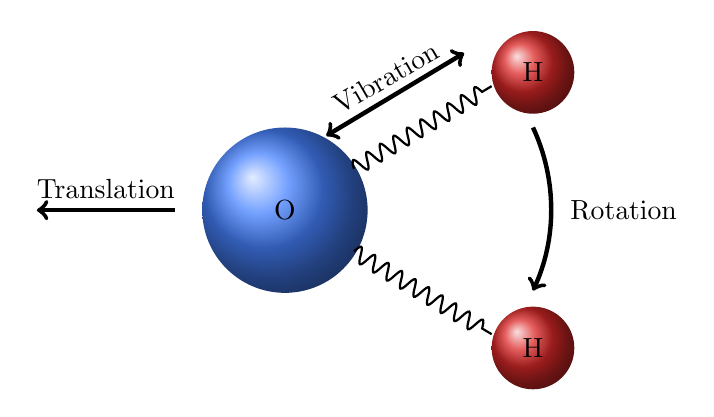
\begin{tikzpicture}[scale=3.5, spring/.style={decorate,decoration={coil,aspect=0,segment length=2mm,amplitude=1mm}}]

  % Oxygen atom color (blue)
  \definecolor{OxyBlue}{RGB}{70,130,255} % light-medium blue
  % Hydrogen atom color (red)
  \definecolor{HydRed}{RGB}{220,40,40}   % bright red

  % Oxygen atom
  \shade[ball color=OxyBlue] (0,0) circle (0.3);

  % Hydrogen atoms (approx 104° apart)
  \shade[ball color=HydRed] (0.9,0.5) circle (0.15);
  \shade[ball color=HydRed] (0.9,-0.5) circle (0.15);
  
  \node at (0,0) {O};
  \node at (0.9,0.5) {H};
  \node at (0.9,-0.5) {H};
  
  \draw[spring,thick] (0.25,0.15) -- (0.75,0.45);
  \draw[spring,thick] (0.25,-0.15) -- (0.75,-0.45);
  
  \onslide<2,5->{
  \draw[->, ultra thick] (-0.4,0) -- (-0.65,0) node[above]{Translation} -- (-0.9,0);
  }
  
  \onslide<3,5->{
  \draw[->,thick, ultra thick] (0.9,0.3) arc[start angle=25,end angle=-25,radius=.7];
  \node at (1., 0) [right]{Rotation};
  %\draw[bend right, ->, ultra thick] (0.9,-0.5) -- (0.9,0.5);
  }
  
  \onslide<4,5->{
  \draw[<->,thick, ultra thick] (0.15,0.27) -- (0.65,0.57);
  \node at (0.4, .42) [above, rotate=30] {Vibration};
  %\draw[bend right, ->, ultra thick] (0.9,-0.5) -- (0.9,0.5);
  }

  % Optional arrows to mimic rotation (as in your image)
  %\draw[->,thick] (0.35,0.55) arc[start angle=100,end angle=20,radius=0.6];
  %\draw[->,thick] (0.35,-0.55) arc[start angle=-100,end angle=-20,radius=0.6];

\end{tikzpicture}
\end{center}

%Les molécules vibrent, tournent et se déplacent de plus en plus vite. Les electrons sont excités jusqu'à ce que certains se détachent et se meuvent librement.
\end{frame}

\begin{frame}{Excitation et ionization}

\begin{center}
\begin{tikzpicture}[scale=3.5, spring/.style={decorate,decoration={coil,aspect=0,segment length=2mm,amplitude=1mm}}]

  % Oxygen atom color (blue)
  \definecolor{OxyBlue}{RGB}{70,130,255} % light-medium blue
  % Hydrogen atom color (red)
  \definecolor{HydRed}{RGB}{220,40,40}   % bright red

  % Oxygen atom
  \shade[ball color=HydRed] (0,0) circle (0.2);
  
  \node at (0,0) {H};
 
  \onslide<2->
  {
  	\def\dist{1.5}
  	\fill[blue] (\dist,0) circle (0.03) node[below left=2pt] {$p^+$};

  	% Orbit path (optional, dashed)
  	\draw[dashed,gray] (\dist,0) circle (.5);

	\draw[->, ultra thick] (.4, 0) -- (.9,0);

  	% Electron (red dot on orbit)
  	\def\ang{40} % position angle
  }
  
  \onslide<2>{
  	\fill[red] ({\dist+.5*cos(\ang)},{.5*sin(\ang)}) circle (0.03) 
  	node[below left] {$e^-$};
  }
  
  \onslide<3->
  {
  	\fill[red!50] ({\dist+.5*cos(\ang)},{.5*sin(\ang)}) circle (0.03) 
  	node[below left] {$e^-$};
  }  
  
  \onslide<3>
  {
  	\draw[dashed,gray] (\dist,0) circle (.7);
  	\fill[red] ({\dist+.7*cos(\ang)},{.7*sin(\ang)}) circle (0.03) 
  	node[above right] {$e^-$};
  	\draw[->, ultra thick, red] ({\dist+.55*cos(\ang)},{.55*sin(\ang)}) -- ({\dist+.65*cos(\ang)},{.65*sin(\ang)});
  }
  
  
  \onslide<4>
  {
  	%\draw[dashed,gray] (\dist,0) circle (.9);
  	\fill[red] ({\dist+.9*cos(\ang)},{.9*sin(\ang)}) circle (0.03) 
  	node[above right] {$e^-$};
  	\draw[->, ultra thick, red] ({\dist+.9*cos(\ang)+0.1},{.9*sin(\ang)}) -- ({\dist+.9*cos(\ang)+0.1+0.5},{.9*sin(\ang)});
  }

\end{tikzpicture}

\only<3>
{
	\begin{framed}
	\centering
	Si l'énergie reçue le permet, l'électron est dans un état \textcolor{red}{\textbf{excité}}. Il reviendra à son état initial en émettant de la lumière: c'est la \textbf{\textcolor{red}{radiation}}.
	\end{framed}
}

\only<4>
{
	\begin{framed}
	\centering
	Si l'énergie reçue est trop grande, l'électron est arraché: il devient \textcolor{red}{\textbf{libre}}. L'atome d'hydrogène a été \textbf{\textcolor{red}{ionisé}}.
	\end{framed}
}

\end{center}

\end{frame}

\begin{frame}{Plasma: le quatrième état de la matière}
\centering
\begin{tabular}{cc}
\begin{tikzpicture}
\node at (0,0) {\includegraphics[height=.3\linewidth]{eau_gaz.png}};
\end{tikzpicture}
&
\onslide<2->
{
\begin{tikzpicture}
\node at (0,0) {\includegraphics[height=.3\linewidth]{eau_gaz.png}};
\fill[red] (0,0) circle (0.1) node[above right] {$e^-$};
\fill[red] (1,1) circle (0.1) node[above right] {$e^-$};
\fill[red] (-1,-0.3) circle (0.1) node[above right] {$e^-$};
\node[blue] at (-1.7,.7) {\textbf{+}};
\node[blue] at (1.4,0) {\textbf{+}};
\end{tikzpicture}
}\\
\textbf{Gaz neutre} & \onslide<2->{\textbf{Plasma}}
\end{tabular}

\only<3>{
\begin{framed}
\textbf{Un plasma est un gaz quasi-neutre composé de particules chargées (ions $\textcolor{blue}{\bullet^+}$ et electrons $\textcolor{red}{\bullet^{e^-}}$) et neutres ($\bullet^n$) démontrant un comportement collectif.\footnotemark}
%A plasma is a quasi-neutral gas of charged and neutral particles which exhibits collective behaviour.
\end{framed}
}
\only<3>{\footnotetext[1]{\tiny F. F. Chen. Introduction to Plasma Physics and Controlled Fusion. Ed. by Springer International Publisher. 2016}}

\end{frame}

\begin{frame}{Comportement collectif du plasma}
\centering
\begin{framed}
\textbf{Collision = interaction entre particules}
\end{framed}

\begin{tabular}{cc}
\onslide<2->{\textbf{Collisions de courte portée}} & \onslide<3->{\textbf{Collisions de longue portée}}\\
\onslide<2->{
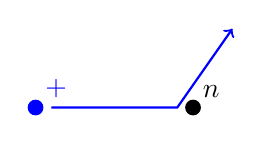
\begin{tikzpicture}
\fill[blue] (0,0) circle (0.1) node[above right] {$+$};
\fill[black] (2,0) circle (0.1) node[above right]{$n$};
\draw[blue, ->, thick] (0.2,0) -- (1.8, 0) -- (2.5, 1);
\end{tikzpicture}} &
\onslide<3->{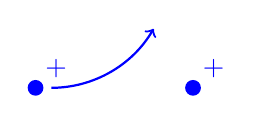
\begin{tikzpicture}
\fill[blue] (0,0) circle (0.1) node[above right] {$+$};
\fill[blue] (2,0) circle (0.1) node[above right] {$+$};
\draw[->,blue, thick] (0.2,0) arc[start angle=-90,end angle=-30,radius=1.5];
\end{tikzpicture}}\\
\onslide<2->{Contact direct (local \& binaire)} & \onslide<3->{Force électrique (à distance, collectif)}
\end{tabular}
\onslide<4->{
\begin{framed}
Si l'échelle est suffisamment grande ($> \SI{1}{\micro\meter}$ dans notre cas), le plasma est \textbf{\textcolor{red}{quasi-neutre}} grâce à la force électrique.
\end{framed}
}
\end{frame}

\begin{frame}{Chimie dans les plasmas}

\begin{framed}
\centering
\textbf{Les collisions entre les particles peuvent mener à des réactions chimiques.}
%\begin{equation*}
%A \leftrightharpoons B
%\end{equation*}
\end{framed}

Si $\tau_{chem}$ et $\tau_{hydro}$ sont les temps caractéristiques de réaction chimique et d'écoulement:
\begin{center}
\begin{tabular}{ccc}
\onslide<2->{$\tau_{chem} \gg \tau_{hydro}$} & \onslide<3->{$\tau_{chem} \simeq \tau_{hydro}$} & \onslide<4->{$\tau_{chem} \ll \tau_{hydro}$}\\
%$A \leftrightharpoons B$ & $A \leftrightharpoons B$ & $A \leftrightharpoons B$\\
\onslide<2->{En équilibre chimique} & \onslide<3->{Hors équilibre chimique} & \onslide<4->{Pas de réaction chimique}\\
\end{tabular}
\end{center}

\onslide<5->{\textbf{Les plasmas sont soit en équilibre, soit hors équilibre.}}

\end{frame}

\begin{frame}{Plasma dans la vie de tous les jours}

\begin{framed}
\centering
\textbf{Les plasmas composent 90\% de l'univers visible.}
\end{framed}
\begin{center}
\includegraphics[height=.22\linewidth]{./sun.jpg}
\includegraphics[height=.22\linewidth]{./aurora_borealis.jpeg}
\includegraphics[height=.22\linewidth]{./lightning.jpg}
\end{center}
De plus en plus d'applications: fusion nucléaire, médecine, métallurgie, lasers, création de microprocesseurs, ...
\end{frame}

\begin{frame}{Plasma froids}

\begin{framed}
\textbf{Pour les plasma froids, l'énergie est d'abord emmagasinée par les électrons libres et cédée lors des collisions aux ions et neutres lourds.}
\end{framed}
%En fonction de l'efficacité des collisions, deux scénarii sont possibles:
\begin{center}
\begin{tabular}{cc}
\onslide<2->{\textbf{Collisions peu efficaces}} & \onslide<3->{\textbf{Collisions efficaces}}\\
\onslide<2->{
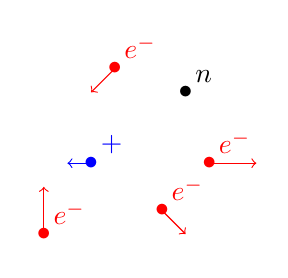
\begin{tikzpicture}[scale=3]
\node[blue] at (0,0) {$\bullet$};
\node at (.4,.3) {$\bullet$};
\node[red] at (.5,0) {$\bullet$};
\node[red] at (.3,-.2) {$\bullet$};
\node[red] at (-.2,-.3) {$\bullet$};
\node[red] at (.1,.4) {$\bullet$};
\draw[red, ->] (.5,0.) -- (.7, 0.);
\draw[red, ->] (.3,-.2) -- (.4, -.3);
\draw[red, ->] (-.2,-.3) -- (-.2, -.1);
\draw[red, ->] (.1,.4) -- (0., .3);
\draw[blue, ->] (0,0) -- (-0.1,0);
\node[blue] at (0,0) [above right]{$+$};
\node at (.4,.3) [above right]{$n$};
\node[red] at (.5,0) [above right]{$e^-$};
\node[red] at (.3,-.2) [above right]{$e^-$};
\node[red] at (-.2,-.3) [above right]{$e^-$};
\node[red] at (.1,.4) [above right]{$e^-$};
\end{tikzpicture}
}
 &
\onslide<3->{
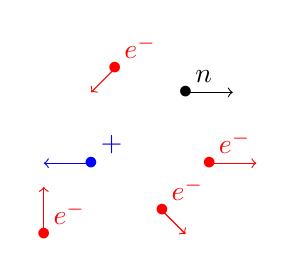
\begin{tikzpicture}[scale=3]
\node[blue] at (0,0) {$\bullet$};
\node at (.4,.3) {$\bullet$};
\node[red] at (.5,0) {$\bullet$};
\node[red] at (.3,-.2) {$\bullet$};
\node[red] at (-.2,-.3) {$\bullet$};
\node[red] at (.1,.4) {$\bullet$};
\draw[red, ->] (.5,0.) -- (.7, 0.);
\draw[red, ->] (.3,-.2) -- (.4, -.3);
\draw[red, ->] (-.2,-.3) -- (-.2, -.1);
\draw[red, ->] (.1,.4) -- (0., .3);
\draw[blue, ->] (0,0) -- (-0.2,0);
\draw[->] (.4,.3) -- (.6,.3);
\node[blue] at (0,0) [above right]{$+$};
\node at (.4,.3) [above right]{$n$};
\node[red] at (.5,0) [above right]{$e^-$};
\node[red] at (.3,-.2) [above right]{$e^-$};
\node[red] at (-.2,-.3) [above right]{$e^-$};
\node[red] at (.1,.4) [above right]{$e^-$};
\end{tikzpicture}}\\
\onslide<2->{Hors équilibre thermique} & \onslide<3->{Equilibre thermique}
\end{tabular}
\end{center}


\end{frame}

\begin{frame}{Plasma en réentrée atmosphérique}
\centering
\includegraphics[height=.35\linewidth]{./reentry_esa.jpg}
\begin{framed}
La grande vitesse de réentrée $\simeq\SI{10}{\kilo\meter\;\second^{-1}}$, un choc suffisamment fort pour ioniser l'air $\Rightarrow$ plasma.
\end{framed}
\end{frame}

\begin{frame}{Sytème de protection thermique et destruction des déchets spatiaux}
\centering
\begin{tabular}{cc}
\onslide<2->{\includegraphics[height=.3\linewidth]{./heat_shield.jpg}} &
\onslide<3->{\includegraphics[height=.3\linewidth]{./vizualisation_satellites_esa.jpg}}\\
\onslide<2->{\textbf{TPS}} & \onslide<3->{\textbf{Déchets spatiaux}}
\end{tabular}
\onslide<4->{
\begin{framed}
\textbf{Nécessité de développer des machines expérimentales reproduisant les plasmas de réentrée atmosphérique pour étudier ces applications.}
\end{framed}
}
\end{frame}

\begin{frame}{Plasma à induction}
\begin{minipage}[t]{0.5\linewidth}
    \centering
    \vspace{0.7cm}
    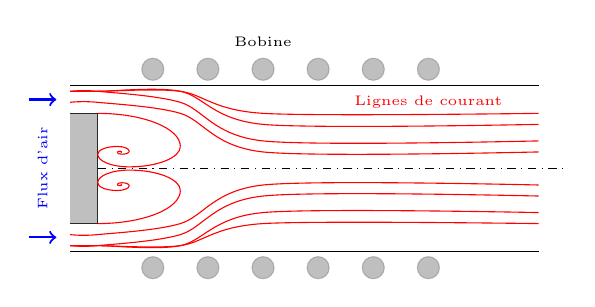
\begin{tikzpicture}[scale=0.7]
      \draw[dash dot] (0,0) -- (8.5,0);
      \draw[-] (-0.5,-1) -- (0, -1) -- (0,1) -- (-0.5,1);
      \fill[gray, opacity=0.5] (-0.5,-1) -- (0, -1) -- (0,1) -- (-0.5,1) -- (-0.5,-1);
      \draw[-] (-0.5,1.5) -- (8,1.5);
      \draw[-] (-0.5,-1.5) -- (8,-1.5);
      \foreach \x in {1,2,...,6}{
        \filldraw[gray, opacity = 0.5] (\x, 1.8) circle (0.2);
        \filldraw[gray, opacity = 0.5] (\x, -1.8) circle (0.2);
      }
      \begin{scope}[red]
      \begin{scope}[yshift=1cm,yscale=-0.6,xscale=1.5]
      \spiral{10}
      \end{scope}
      \begin{scope}[yshift=-1cm,yscale=0.6,xscale=1.5]
      \spiral{10}
      \end{scope}
      \draw plot [help lines, smooth] coordinates {(-0.5,1.2) (0,1.2) (1.5, 1.0) (3, 0.3) (8, 0.3)};
      \draw plot [help lines, smooth] coordinates {(-0.5, -1.2) (0,-1.2) (1.5, -1.0) (3, -0.3) (8, -0.3)};
      
      \draw plot [help lines, smooth] coordinates {(-0.5, 1.4) (0,1.4) (1.5, 1.2) (3, 0.5) (8, 0.5)};
      \draw plot [help lines, smooth] coordinates {(-0.5, -1.4) (0,-1.4) (1.5, -1.2) (3, -0.5) (8, -0.5)};
      
      \draw plot [help lines, smooth] coordinates {(-0.5, 1.4) (0, 1.4) (1.5, 1.4) (3, 0.8) (8, 0.8)};
      \draw plot [help lines, smooth] coordinates {(-0.5, -1.4) (0, -1.4) (1.5, -1.4) (3, -0.8) (8, -0.8)};
      
      \draw plot [help lines, smooth] coordinates {(-0.5, 1.4) (0, 1.4) (1.5, 1.4) (3, 1.0) (8, 1.0)};
      \draw plot [help lines, smooth] coordinates {(-0.5, -1.4) (0, -1.4) (1.5, -1.4) (3, -1.0) (8, -1.0)};
      
      \draw (6,1.2) node{\tiny \textcolor{red}{Lignes de courant}};
      \draw (3,2.3) node{\tiny \textcolor{black}{Bobine}};
      \draw (-1,0) node{\tiny \rotatebox{90}{\textcolor{blue}{Flux d'air}}};
      \end{scope}
      
      %\draw (2,0.2) node{$T\simeq \SI{}{10^4\kelvin}$};
      \draw[blue, ->, thick](-1.25, 1.25) -- (-0.75,1.25);
      \draw[blue, ->, thick](-1.25, -1.25) -- (-0.75,-1.25);
      %\draw (3.5,2.3) node{\includegraphics[width=0.1\linewidth]{AC_Sign.png}};
      %\draw (6,1.2) node{$p \simeq \SI{}{10^4\pascal}$};
      
    \end{tikzpicture}
    
    \vspace{0.45cm}
    Torche
    \end{minipage}
    \begin{minipage}[t]{0.49\linewidth}
    \centering
    \vspace{0.5cm}\includegraphics[width=\linewidth]{Ablation-testing-at-the-Plasmatron-ICP-facility-of-the-VKI-3.jpg}
    
    Chambre
    \end{minipage}
    
    \only<1>
    {
    Examples: Plasmatron (VKI), Plasmatron X (Illinois), IPG (Russie), ...
    
    Basé sur le principe de \textbf{transfer de chaleur local}.
    }
    \only<2>
    {
    	Résoudre les équations de Maxwell, de Navier-Stokes + modèles physico-chimiques + modèle de radiation.
    }
    %Physique de l'électromagnétisme, equations de la mécanique des fluides, et chimie/thermodynamique.
\end{frame}

\begin{frame}{Plasma à induction: besoin de plus}

\begin{center}
\begin{framed}
\textbf{Des solvers numériques (volumes finis) ont été développés afin de préparer au mieux les expériences dans les torches à induction.}
\end{framed}
\includegraphics[width=.7\linewidth]{lhtsT.pdf}\footnote{\tiny Thierry Magin.}
\end{center}
\end{frame}

\begin{frame}{Motivations de la thèse}
%\begin{framed}
%\centering
%\textbf{La plupart des solvers représentent des écoulements axisymmétriques en régime établi avec un modèle chimique et thermique d'équilibre.}
%\end{framed}

\textbf{La plupart des solvers actuels}

\begin{itemize}
\item \onslide<2->{Ne représentent que des géométries axisymmétriques et simples.}

\only<2>{
\begin{center}
\includegraphics[width=.7\linewidth]{lhtsT.pdf}
\end{center}
}

\only<3>{

\begin{center}
\includegraphics[height=.23\linewidth]{./coil_effect.png}
\includegraphics[height = .23\linewidth]{./plasmatron_nozzle_operating.png}
\includegraphics[height = .23\linewidth]{./plasmatron_nozzles.png}
\end{center}
}

\onslide<4->{\textit{Besoin d'un solver 3D.}}

\item \onslide<5-> {Sont en régime établi.}

\only<6>
{
\begin{center}
\includegraphics[height=.2\linewidth]{./plasma_jet_unsteady_experimental.png}
\end{center}
}

\onslide<7-> {\textit{Besoin d'un solver instationnaire.}}

\item \onslide<8-> {Utilisent un modèle à l'équilibre chimique et thermique sans radiation.}

\only<9>{
\textit{C'est faux! Car la les déséquilibre chimique et thermique ont été observés dans les plasma à induction! La radiation joue aussi un rôle important dans le transfer de chaleur.}
}

\onslide<10->{
\textit{Besoin d'un solver avec une chimie plus détaillée et de la radiation.}
}

\end{itemize}

\onslide<11->{
\begin{framed}
\textbf{Peut-on améliorer les solvers volume finis actuels afin de pouvoir prendre en compte toute la physique?}
\end{framed}
}

\end{frame}

\begin{frame}{Le problème des solvers volume finis actuels.}

\begin{center}
\includegraphics[width=.65\linewidth]{./thierry_mesh.png}
\reflectbox{\includegraphics[width = .65\linewidth, angle=180, origin=c]{./thierry_mesh.png}}
\end{center}

\only<1>{
\begin{center}
\includegraphics[width=.65\linewidth]{lhtsT.pdf}
\end{center}

Pour les volumes finis, la solution est constante sur chaque éléments.

}

\onslide<2->
{
\begin{framed}
\textbf{Les volumes finis nécessitent un maillage de bonne qualité, et donc très fin dans les régions de grande variation ou de géométrie complexe $\Rightarrow$}
\end{framed}

\begin{itemize}
\item Demande beaucoup d'attention au maillage.
\item Quasi impossible pour les géométries complexes.
\item Demande un maillage trop fin partout pour une physique plus complexe.
\end{itemize}

}

\end{frame}

\begin{frame}{But de la thèse}

\begin{framed}
\textbf{Développer un solver faisant partie des méthodes de Galerkin discontinues pour les plasma à induction.}
\end{framed}

\begin{itemize}
\item La solution n'est plus constante sur chaque élément.
\item Beaucoup plus grande flexibilité de maillage.
\end{itemize}

\begin{center}
\includegraphics[width=.8\linewidth]{./Grid_Independence_mesh_probe_cropped.pdf}
\reflectbox{\includegraphics[width = .8\linewidth, angle=180, origin=c]{./Grid_Independence_mesh_probe_cropped.pdf}}
\end{center}

\end{frame}

\begin{frame}{Research questions}

With the objective of producing a new high order solver for inductively coupled plasma, we will try to answer the following questions:

\begin{framed}
\begin{description}
\item[Q1] \textbf{In addition of being precise, can a high-order solver be robust for inductively coupled plasma applications?}
\item[Q2] \textbf{Is the developed solver user-friendly?} 
\item[Q3] \textbf{Can the new solver be easily adapted to the new experiments performed in ICP facilities?}
\end{description}
\end{framed}

\end{frame}

\section{Model for inductively coupled plasma}

\begin{frame}{Hypothesis on the plasma}

%\begin{framed}
%
%\textbf{In order to simplify the development of the solver, assumptions are made.}
%\end{framed}
\begin{minipage}{.6\linewidth}
%\small
\onslide<1->
{
\textbf{Collision-dominated and thermal plasma}
}

\onslide<2->
{
\textbf{Quasi-neutrality}
}

\onslide<3->
{
\textbf{No displacement current}
}

\onslide<4->
{
\textbf{Axisymmetry}
}

\onslide<5->
{
\textbf{Non-radiative plasma}
}

\onslide<6->
{
\textbf{Local thermodynamic equilibrium}
}

\onslide<7->
{
\textbf{No elemental de-mixing}
}

\onslide<8->
{
\textbf{Unmagnetized plasma}
}

\onslide<9->
{
\textbf{Steady-state}
}
\end{minipage}
\begin{minipage}{.39\linewidth}
\only<1>{
\begin{center}
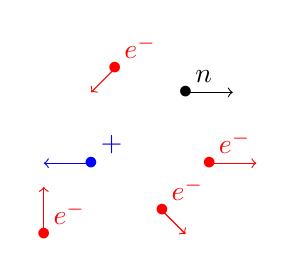
\begin{tikzpicture}[scale=3]
\node[blue] at (0,0) {$\bullet$};
\node at (.4,.3) {$\bullet$};
\node[red] at (.5,0) {$\bullet$};
\node[red] at (.3,-.2) {$\bullet$};
\node[red] at (-.2,-.3) {$\bullet$};
\node[red] at (.1,.4) {$\bullet$};
\draw[red, ->] (.5,0.) -- (.7, 0.);
\draw[red, ->] (.3,-.2) -- (.4, -.3);
\draw[red, ->] (-.2,-.3) -- (-.2, -.1);
\draw[red, ->] (.1,.4) -- (0., .3);
\draw[blue, ->] (0,0) -- (-0.2,0);
\draw[->] (.4,.3) -- (.6,.3);
\node[blue] at (0,0) [above right]{$+$};
\node at (.4,.3) [above right]{$n$};
\node[red] at (.5,0) [above right]{$e^-$};
\node[red] at (.3,-.2) [above right]{$e^-$};
\node[red] at (-.2,-.3) [above right]{$e^-$};
\node[red] at (.1,.4) [above right]{$e^-$};
\end{tikzpicture}

\begin{framed}
\begin{equation*}
T_e \simeq T_h
\end{equation*}
\end{framed}

\end{center}
}

\only<2>
{

Characteristic length greater than the Debye length, \textit{i.e.} the distance at which
\begin{equation*}
E_{thermal} \simeq E_{elec}
\end{equation*}
so
\begin{equation*}
q \simeq 0
\end{equation*}

}

\only<3>
{

	ELM waves perturb electrons, but they are assumed to return fast to equilibrium.
	
	ELM wavelength are much greater than the plasma length scale.

}

\only<4>
{

%	No 3D plasma modes may occur.
%	Fully axisymmetric electric field.
	
	\begin{center}
	\includegraphics[height=.4\linewidth]{./coil_effect.png}
	\includegraphics[height = .4\linewidth]{./plasmatron_nozzle_operating.png}
	\includegraphics[height = .4\linewidth]{./plasmatron_nozzles.png}
	\end{center}

}

\only<5>
{
	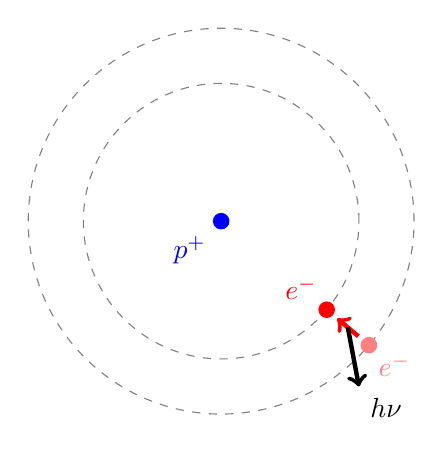
\begin{tikzpicture}[scale=3.5]
	\def\dist{1.5}
  	\fill[blue] (\dist,0) circle (0.03) node[below left=2pt] {$p^+$};

  	% Orbit path (optional, dashed)
  	\draw[dashed,gray] (\dist,0) circle (.5);

  	% Electron (red dot on orbit)
  	\def\ang{-40} % position angle
  
  
  	\fill[red] ({\dist+.5*cos(\ang)},{.5*sin(\ang)}) circle (0.03) 
  	node[above left] {$e^-$};
    
  	\draw[dashed,gray] (\dist,0) circle (.7);
  	\fill[red!50] ({\dist+.7*cos(\ang)},{.7*sin(\ang)}) circle (0.03) 
  	node[below right] {$e^-$};
  	\draw[<-, ultra thick, red] ({\dist+.55*cos(\ang)},{.55*sin(\ang)}) -- ({\dist+.65*cos(\ang)},{.65*sin(\ang)});
  	
  	\draw[->, ultra thick] ({\dist+.6*cos(\ang)}, {.6*sin(\ang)}) -- (2., -.6) node[below right]{$h \nu$};
  
  \end{tikzpicture}
}

\only<6>
{

Chemical reaction return very fast to equilibrium.

In reality, non equilibrium can be observed in the torch.

Thermal + chemical equilibrium = local thermodynamic equilibrium.

}

\only<7>
{

Elemental de-mixing accounts for the diffusion of elements. In the case of LTE, gives results closer to non-equilibrium models.

Cheaper to solve as the elements have no production rates. 

}

\only<8>
{
\includegraphics[width=.7\linewidth]{helicoidal_motion.png}
}

\only<9>
{
\includegraphics[width=\linewidth]{./plasma_jet_unsteady_experimental.png}

We average the equations over one period of the induction current. 
}

\only<10>
{
The electric field:

\begin{itemize}

\item It is ambipolar ($j_z = j_r = 0$).

\item The coils are thin parallels wires surrounding the facility.

\item Axisymmetric

\item $E_{tot} = E_C + E_P$

\item We use phasor notation.

\end{itemize}
}

\end{minipage}

\end{frame}

\begin{frame}{Equations governing the plasma}

\textbf{Navier-Stokes equations}

\begin{framed}
\begin{equation*}
\begin{aligned}
& \partial_t \rho + \nabla \cdot \left(\rho \vecv\right) = 0\\
& \partial_t \left(\rho \vecv\right) + \nabla \cdot \left(\rho \vecv \vecv \right) = -\nabla p + \nabla \cdot \vectau + \vecF_L\\
& \partial_t \left(\rho e + \frac{1}{2} \rho ||\vecv||^2\right) + \nabla \cdot \left(\rho e \vecv + \frac{1}{2} \rho ||\vecv||^2 \vecv + p \vecv\right) = \nabla \cdot \left(\vectau\vecv\right) + \nabla \cdot \vecq + P_J\\
\end{aligned}
\end{equation*}
\end{framed}

\only<2>
{
\vspace{-.7cm}
\begin{minipage}{0.49\linewidth}
\begin{equation*}
\begin{aligned}
& \vectau = \eta \left(\nabla \vecv + \nabla \vecv^T\right) - \frac{2}{3} \eta \nabla \cdot \vecv\\
& \vecq = -k \nabla T
\end{aligned}
\end{equation*}
\end{minipage}
\begin{minipage}{0.49\linewidth}
\begin{equation*}
\begin{aligned}
& F_z^L = \frac{\sigma_e}{4 \pi f} \left[E_I^{Im} \partial_z E_I^{Re} - E_I^{Re} \partial_z E_I^{Im}\right]\\
& F_r^L = \frac{\sigma_e}{4 \pi f} \left[E_I^{Im} \frac{1}{r}\partial_r (r E_I^{Re}) - E_I^{Re} \frac{1}{r} \partial_r (r E_I^{Im})\right]\\
& P^J = \frac{\sigma_e}{2} \left[(E_I^{Im})^2 + (E_I^{Re})^2\right]
\end{aligned}
\end{equation*}
\end{minipage}
}

\end{frame}

\begin{frame}{Electric field equation}

\begin{framed}
\begin{equation*}
\partial^2_{zz} E_P + \frac{1}{r}\partial_r (r \partial_r E_P) - \frac{E_P}{r^2} = i 2 \pi f\mu_0\sigma_e \left(E_C + E_P\right)
\end{equation*}
\end{framed}

\only<2>
{
$\mu_0$ : magnetic permeability

$\sigma_e$ : electron electric conductivity

$f$ : induction frequency
}

\only<3>
{
\begin{equation*}
	E_C = \sum_{l=1}^{N_{coil}} i f \mu_0 I_C \sqrt{\frac{r_0}{r}}\left[2 \frac{E_2(k_l)}{k_l} - E_1(k_l)\left(\frac{2}{k_l}-k_l\right)\right]
\end{equation*}
\begin{equation*}
		E_1(k) = \int_0^{\frac{\pi}{2}} \frac{d\theta}{\sqrt{1-k^2 \sin^2(\theta)}} \quad E_2(k) = \int_0^{\frac{\pi}{2}} \sqrt{1-k^2 \sin^2(\theta)} \; d\theta
\end{equation*}
}

\end{frame}

\begin{frame}{Transport properties}

\begin{framed}
\centering
\textbf{The transport properties are computed using Mutation++}

$\eta$, $k$, $\sigma_e$ 
\end{framed}

\begin{center}
\includegraphics[width=\linewidth]{./mpp-logo.png}
\end{center}

\end{frame}

\begin{frame}{Coupling of the systems}

\only<1,2>
{
\textbf{Navier-Stokes}
\begin{equation*}
\begin{aligned}
& \partial_t \rho + \nabla \cdot \left(\rho \vecv\right) = 0\\
& \partial_t \left(\rho \vecv\right) + \nabla \cdot \left(\rho \vecv \vecv \right) = -\nabla p + \nabla \cdot \vectau + \vecF_L\\
& \partial_t \left(\rho e + \frac{1}{2} \rho ||\vecv||^2\right) + \nabla \cdot \left(\rho e \vecv + \frac{1}{2} \rho ||\vecv||^2 \vecv + p \vecv\right) = \nabla \cdot \left(\vectau\vecv\right) + \nabla \cdot \vecq + P_J\\
\end{aligned}
\end{equation*}
}

\only<2>
{
\textbf{Maxwell}
\begin{equation*}
\begin{aligned}
& \partial^2_{zz} E_P + \frac{1}{r}\partial_r (r \partial_r E_P) - \frac{E_P}{r^2} = i 2 \pi f\mu_0\sigma_e \left(E_C + E_P\right)
\end{aligned}
\end{equation*}
}

\only<3>
{
\textbf{Navier-Stokes}
\begin{equation*}
\begin{aligned}
& \partial_t \rho + \nabla \cdot \left(\rho \vecv\right) = 0\\
& \partial_t \left(\rho \vecv\right) + \nabla \cdot \left(\rho \vecv \vecv \right) = -\nabla p + \nabla \cdot \vectau + \textcolor{red}{\vecF_L}\\
& \partial_t \left(\rho e + \frac{1}{2} \rho ||\vecv||^2\right) + \nabla \cdot \left(\rho e \vecv + \frac{1}{2} \rho ||\vecv||^2 \vecv + p \vecv\right) = \nabla \cdot \left(\vectau\vecv\right) + \nabla \cdot \vecq + \textcolor{red}{P_J}\\
\end{aligned}
\end{equation*}

\textbf{Maxwell}
\begin{equation*}
\begin{aligned}
& \partial^2_{zz} E_P + \frac{1}{r}\partial_r (r \partial_r E_P) - \frac{E_P}{r^2} = i 2 \pi f\mu_0\textcolor{red}{\sigma_e} \left(E_C + E_P\right)
\end{aligned}
\end{equation*}
}

\end{frame}

\begin{frame}{Computational domain}

\begin{center}
\begin{tikzpicture}[scale = .6]
	\draw[dash dot] (-1.0,0) -- (15,0);
	\draw[-, thick] (-1.0,-1) -- (0, -1) -- (0,1) -- (-1.0,1);
	\fill[gray, opacity=0.5] (-1.0,-1) -- (0, -1) -- (0,1) -- (-1.0,1) -- (-1.0,-1);
	\draw[-,thick] (-1.0,1.5) -- (8.5,1.5) -- (8.5,4.);
	\draw[-,thick] (-1.0,-1.5) -- (8.5,-1.5) -- (8.5,-4);
	\foreach \x in {1,2,...,6}{
		\filldraw[gray, opacity = 0.5] (\x, 2.) circle (0.2);
		\filldraw[gray, opacity = 0.5] (\x, -2.) circle (0.2);
	}
	\draw[dashed, blue] (0.2, 0) -- (0.2, 1.3) -- (8.7, 1.3) -- (8.7, 3.8) -- (15, 3.8) -- (15, 0.7) -- (13, 0.7) arc[start angle=90, end angle = 180, radius=0.7];
	\draw[dashed, blue] (0.2, 0) -- (0.2, -1.3) -- (8.7, -1.3) -- (8.7, -3.8) -- (15, -3.8) -- (15, -0.7) -- (13, -0.7) arc[start angle=-90, end angle = -180, radius=0.7];
	\draw[blue] (7,0) node[above]{Maxwell + N-S};
	\draw[dashed, red] (-1.2,0) -- (-1.2, 1.7) -- (8, 1.7) -- (8, 3.8) -- (-3, 3.8) -- (-3,0);
	\draw[dashed, red] (-1.2,0) -- (-1.2, -1.7) -- (8, -1.7) -- (8, -3.8) -- (-3, -3.8) -- (-3,0);
	\draw[red] (3.5,-3) node[above]{Maxwell};
	\draw[-, thick] (15, 0.5) -- (13,0.5) arc[start angle=90, end angle = 180, radius=0.5];
	\draw[-, thick] (15, -0.5) -- (13,-0.5) arc[start angle=-90, end angle = -180, radius=0.5];
	%\draw (14,-0.15) node[above]{Probe};
	
	\only<6,9>
	{
	\draw[-, thick, black, ->] (-1, 1.25) -- (-0.2, 1.25);
	\draw[-, thick, black, ->] (-1, -1.25) -- (-0.2, -1.25);
	}
	
	% Boundary conditions
	
	\only<4,9>{\draw (12,3.8) node[above]{Opening}};
	\only<4,9>{\draw (15,2) node[above, rotate = -90]{Opening}};
	\only<3,9>{\draw (4,3.8) node[above]{Far electric field};}
	\only<3,9>{\draw (-3,0) node[above, rotate = 90]{Far electric field};}
	\only<5,9>{\draw (0.2,0) node[above, rotate = -90]{Isothermal}};
	\only<5,9>{\draw (4,-1.3) node[above]{No slip isothermal}};
	\only<5,9>{\draw (14, -0.7) node[below]{Isothermal}};
	\only<7,9>{\draw (8.7, -2.55) node[above, rotate = -90] {Coflow}};
	
\end{tikzpicture}
\end{center}

\only<2>
{
\textbf{Symmetry axis} $\partial_r p = 0$, $\partial_r u_z = 0$, $u_r = 0$, $\partial_r T = 0$ and $E_P = 0$.
}
\only<3>
{
\textbf{Vanishing far electric field} $E_P = 0$.
}
\only<4>
{
\textbf{Openings} $p = p_0$
}
\only<5>
{	
\textbf{No-slip wall isothermal} $T = T_{wall}$ and $\vecu = \mathbf{0}$.
}
\only<6>
{
\textbf{Inflow} $u_z = U_{in}$, $u_r = 0$ and $T = T_{inlet}$.
}
\only<7>
{
\textbf{Stabilizing co-flow} $T = T_{wall}$, $\vecu = u_{coflow} \mathbf{e}_z$
}
\only<8>
{
\textbf{ICP and Maxwell interface}
\begin{equation*}
\begin{aligned}
&\nabla E_p^{Re, NS} \cdot \vecn^{NS} &&= \nabla E_p^{Re, MAX} \cdot \vecn^{MAX}\\
&\nabla E_p^{Im, NS} \cdot \vecn^{NS} &&= \nabla E_p^{Im, MAX} \cdot \vecn^{MAX}
\end{aligned}
\end{equation*}
}
\end{frame}

\section{Hybridized discontinuous Galerkin method}

\begin{frame}{Conservative form of the equations}

%\textbf{Navier-Stokes}
\begin{equation*}
\begin{aligned}
& \partial_t \rho &&+ \nabla \cdot \left(\rho \vecv\right) && &&= 0\\
& \partial_t \left(\rho \vecv\right) &&+ \nabla \cdot \left(\rho \vecv \vecv + p \mathbb{I} \right) &&- \nabla \cdot \vectau &&= \vecF_L\\
& \partial_t \left(\rho E\right) &&+ \nabla \cdot \left(\rho E \vecv + p \vecv\right) &&- \nabla \cdot \left(\vectau\vecv + \vecq\right) &&= P_J\\
& && &&- \nabla \cdot \left(\nabla E_P\right) &&= -\frac{E_P}{r^2} - i 2 \pi f\mu_0\sigma_e \left(E_C + E_P\right)\\
& && && &&\\
\only<2>
{
& \partial_t \vecw(\vecu) &&+ \nabla \cdot \vecF_c(\vecu) &&- \nabla \cdot \vecF_v(\vecu, \nabla \vecu) &&= \vecS(\vecu, \nabla \vecu)
}
\end{aligned}
\end{equation*}

\only<3>
{
\begin{framed}
\begin{equation*}
\partial_t \vecw(\vecu) + \nabla \cdot \vecF_c(\vecu) - \nabla \cdot \vecF_v(\vecu, \nabla \vecu) = \vecS(\vecu, \nabla \vecu)
\end{equation*}
\end{framed}
}

%\textbf{Maxwell}
%\begin{equation*}
%\begin{aligned}
%
%\end{aligned}
%\end{equation*}

%\onslide<2>
%{

%}

\end{frame}

\begin{frame}{Finite volume and (hybridized) discontinuous Galerkin}

\centering
\begin{tikzpicture}[scale = 1.5]
	% Define the vertices of the standing on base triangle
    \coordinate (A) at (0, 0, 0);
    \coordinate (B) at (4, 0, 0);
    \coordinate (C) at (2, 0, -3.464); % Height for an equilateral triangle
    
    % Define the vertice of the trace
    \coordinate (D) at (5,0,0);
    \coordinate (E) at (3,0,-3.464);
    
    % Define the vertices of the standing on head triangle
    \coordinate (F) at (6, 0,0);
    \coordinate (G) at (4, 0,-3.464);
    \coordinate (H) at (8, 0,-3.464);

    % Draw the triangle standing on its base
    \draw[thick] (A) -- (B) -- (C) -- cycle;
    
    % Draw the triangle standing on its head
    \draw[thick] (F) -- (G) -- (H) -- cycle;
    
    \only<3->
    {
    % Draw the trace
    \draw[thick] (D) -- (E);
	}
    % Place the nodes at the vertices
    \draw[blue] (A) circle (2pt);
    %\only<1>
    {
    \draw[blue] (B) circle (2pt);
    }
%    \only<2->
%    {
%    \draw[blue] (B) circle (2pt) node[below] {$\vecu_1$, $\vecq_1$};
%	}    
    \draw[blue] (C) circle (2pt);
    
    \only<3->
    {
    \draw[red] (D) circle (2pt);
    \draw[red] (E) circle (2pt);
    }
	%\only<1>
    {
    \draw[blue] (F) circle (2pt);
	}       
    
%    \only<2->
%    {
%    \draw[blue] (F) circle (2pt) node[below] {$\vecu_2$, $\vecq_2$};
%	}    
    \draw[blue] (G) circle (2pt);
    \draw[blue] (H) circle (2pt);

    % Place the mid-edge nodes for the triangle on its basis
    \coordinate (AB) at ($.5*(A)+ 0.5*(B)$);
    \coordinate (BC) at ($.5*(B)+ 0.5*(C)$);
    \coordinate (CA) at ($.5*(C)+ 0.5*(A)$);
    
    \only<3->
    {
    % Place the mid-edge of the trace
    \coordinate (DE) at ($.5*(D)+ 0.5*(E)$);
    }
    
    % Place the mid-edge nodes for the triangle on its head
    \coordinate (FG) at ($.5*(F)+ 0.5*(G)$);
    \coordinate (GH) at ($.5*(G)+ 0.5*(H)$);
    \coordinate (HF) at ($.5*(H)+ 0.5*(F)$);

    \draw[blue] (AB) circle (2pt);
    \draw[blue] (BC) circle (2pt);
    \draw[blue] (CA) circle (2pt);
    
    \draw[blue] (FG) circle (2pt);
    \draw[blue] (GH) circle (2pt);
    \draw[blue] (HF) circle (2pt);
    
    \only<3->
    {
    \draw[red] (DE) circle (2pt);% node[above right] {$\veclambda$};
    \node[below left] at (DE) {$e$};
    }
    % Marks the center of the triangles
    \coordinate (ABC) at ($ .333*(A) + .333*(B) + .333*(C) $);
    \coordinate (FGH) at ($ .333*(F) + .333*(G) + .333*(H) $);
    
    \node[black] at (ABC) {$K_1$};
    \node[black] at (FGH) {$K_2$};
    
    % Shape function of the first element.
    \only<1>{
    \coordinate (I) at (0, 1., 0);
    \coordinate (J) at (4, 1., 0);
    \coordinate (K) at (2, 1., -3.464);
    }
    
    \only<2->{
    	 \coordinate (I) at (0, 1.5, 0);
     \coordinate (J) at (4, 2., 0);
     \coordinate (K) at (2, 1.75, -3.464);
    }
    
    \coordinate (IJ) at (2, 1., 0);
    \coordinate (JK) at (3, 2.5, -1.732);
    \coordinate (KI) at (1, 1.3, -1.732);
    
    \coordinate (IJK) at ($ .333*(I) + .333*(J) + .333*(K) $);
    
    \draw[dashed] (A) -- (I);
    \draw[dashed] (B) -- (J);
    \draw[dashed] (C) -- (K);
    
    \fill[blue] (I) circle (2pt);
    \fill[blue] (J) circle (2pt);
    \fill[blue] (K) circle (2pt);

	\only<1>{
	\fill[smooth, blue!20, opacity=0.5, tension = 0.] (I) -- (J) -- (K);
    \draw[smooth, thick, blue, tension = 0.] (I) -- (J) -- (K) -- cycle;
	}
   
    \only<2->{ 
    \fill[smooth, blue!20, opacity=0.5, tension = 0.] (I) .. controls (IJ) .. (J) -- (J) .. controls (JK) .. (K) -- (K) .. controls (KI) ..(I);
    \draw[smooth, thick, blue, tension = 0.] (I) .. controls (IJ) .. (J) -- (J) .. controls (JK) .. (K) -- (K) .. controls (KI) ..(I);
	}

	\only<1,2>
	{
	\node[below, blue] at (IJK) {$\vecu_{K_1}$};
	}
	
	\only<3->
	{
	\node[below, blue] at (IJK) {$\vecu_{K_1}$, $\vecq_{K_1}$};
	}
	
%	\only<2->
%	{
%	\node[below, blue] at (IJK) {$\varphi_{K_1}$};
%	}
	% Shape function of the second element.
	\only<1>
	{
    \coordinate (L) at (6, 2,0);
    \coordinate (M) at (4, 2,-3.464);
    \coordinate (N) at (8, 2,-3.464);
    }
    
    \only<2->
	{
    \coordinate (L) at (6, 2,0);
    \coordinate (M) at (4, 1.75,-3.464);
    \coordinate (N) at (8, 1.5,-3.464);
    }
    
    \coordinate (LM) at (5, 1.3, -1.732);
    \coordinate (MN) at (6, 2.2, -3.464);
    \coordinate (NL) at (7, 2.3, -1.732);
    
    \coordinate (LMN) at ($ .333*(L) + .333*(M) + .333*(N) $);
    
    \draw[dashed] (F) -- (L);
    \draw[dashed] (G) -- (M);
    \draw[dashed] (H) -- (N);
    
    \fill[blue] (L) circle (2pt);
    \fill[blue] (M) circle (2pt);
    \fill[blue] (N) circle (2pt);

	\only<1>{
	\fill[smooth, blue!20, opacity=0.5, tension = 0.] (L) -- (M) -- (N);
	\draw[smooth, thick, blue, tension = 0.] (L) -- (M) -- (N) -- cycle;
	}    
    
    \only<2->{\fill[smooth, blue!20, opacity=0.5, tension = 0.] (L) .. controls (LM) .. (M) -- (M) .. controls (MN) .. (N) -- (N) .. controls (NL) ..(L);
    \draw[smooth, thick, blue, tension = 0.] (L) .. controls (LM) .. (M) -- (M) .. controls (MN) .. (N) -- (N) .. controls (NL) ..(L);
	}
	\only<1,2>
	{
	\node[above, blue] at (LMN) {$\vecu_{K_2}$};
	}

	\only<3->
	{
	\node[above, blue] at (LMN) {$\vecu_{K_2}$, $\vecq_{K_2}$};
	}	
	
%	\only<2->
%	{
%	\node[above, blue] at (LMN) {$\varphi_{K_2}$};
%	}
	% Shape function of the trace.
	
	\only<3->
	{
	\coordinate (O) at (5,1.7,0);
    \coordinate (P) at (3,2.,-3.464);
    \coordinate (OP) at (4,1.5,-1.732);
    
    \coordinate (OP_Bary) at ($ .5*(O) + .5*(P) $);
    
    \draw[smooth, thick, red, tension = 0.] (O) .. controls (OP) .. (P);
    
    \draw[dashed] (D) -- (O);
    \draw[dashed] (E) -- (P);
    
    \fill[red] (O) circle (2pt);
    \fill[red] (P) circle (2pt);
    
    \node[above right, red] at (OP_Bary) {$\veclambda_e$};
	}
	
	\only<1,2>{

	\draw[<->, ultra thick] ($(BC) + (0.1, 0)$) -- ($.5*(BC) + .5*(FG)$) node[below]{$\vecHcal$} -- ($(FG) - (0.1,0)$);	
	
	}

	\only<3>{

	\draw[<->, ultra thick] ($(BC) + (0.1, 0)$) -- ($.5*(BC) + .5*(DE)$) node[above]{$\vecHcal_1$} -- ($(DE) - (0.1,0)$);
	\draw[<->, ultra thick] ($(DE) + (0.1, 0)$) -- ($.5*(DE) + .5*(FG)$) node[above]{$\vecHcal_2$} -- ($(FG) - (0.1,0)$);	
	
	}	
	
	% Axis
	
	%\draw[->, thick] (0, -2, 0) -- (0, -2, -1.5) node[above]{$\vece_y$};
	%\draw[->, thick] (0, -2, 0) -- (1.5, -2, 0) node[above]{$\vece_x$};
	%\draw[->, thick] (0, -2, 0) -- (0, -0.5, 0) node[right]{$\varphi, \mu$};

\end{tikzpicture}

\only<1>{
\begin{framed}
\centering
\textbf{Finite volumes}
\end{framed}
}

\only<2>{
\begin{framed}
\centering
\textbf{Discontinuous Galerkin}
\end{framed}
}

\only<3>{
\begin{framed}
\centering
\textbf{Hybridized discontinuous Galerkin}
\end{framed}
}

\end{frame}

\begin{frame}{Model problem}

\begin{framed}
\begin{equation*}
	\begin{aligned}
		& \partial_t \vecw(\vecu) + \nabla \cdot \left(\vecF_c(\vecu) - \vecF_v(\vecu, \nabla \vecu)\right) = \vecS(\vecu, \nabla \vecu) && \text{ on } \Omega\\
		& \vecu = \vecu_{bc} && \text{ on } \partial\Omega_D\\
		& \vecF_v \cdot \vecn = \vecF_{v,n,bc} && \text{ on } \partial\Omega_N\\
		& \vecu(t = 0) = \vecU && \text{ on } \Omega
	\end{aligned}
\end{equation*}
\end{framed}

\only<1>{
\begin{minipage}[t]{0.49\linewidth}
$\vecF_{c,v}$ : convective and diffusive fluxes.

$S$ : source terms.

$w$ : conservative variables.

$\vecu$, $\vecu_{bc}$ : solution and boundary condition.
\end{minipage}
\begin{minipage}[t]{0.49\linewidth}
$\Omega$ : domain of the problem.

$\partial\Omega_{D,N}$ : domain boundary for Dirichlet and Neumann BC.

$\vecU$ : initial data.
\end{minipage}
}

\only<2>{
Before going further, some notation:
\begin{equation*}
\begin{aligned}
&(a,b)_{K} &&= \int_K a b\;dV,\\
&\langle a,b \rangle_{\partial K} &&= \int_{\partial K} a  b \;dS.\\
\end{aligned}
\end{equation*}

}

\end{frame}

\begin{frame}{From weak form to discrete DG problem}

\only<1>
{
\begin{equation*}
\left(\partial_t \vecw - \vecS, w \right)_{\Omega} - \left(\vecF_{c} - \vecF_{v}, \nabla w \right)_{\Omega} + \left\langle \left(\vecF_{c} - \vecF_{v}\right) \cdot \vecn, w \right\rangle_{\partial \Omega} = 0, \; \forall w \in L_2(\Omega)
\end{equation*}

Multiplying by a function $w \in L_2(\Omega)$ and integrating over the domain gives the \textbf{weak form}.
}

\only<2>
{
\begin{equation*}
\left(\partial_t \vecw - \vecS, w \right)_{\textcolor{red}{\tesselation}} - \left(\vecF_{c} - \vecF_{v}, \nabla w \right)_{\textcolor{red}{\tesselation}} + \textcolor{red}{\sum_{K \in \tesselation}} \left\langle \left(\vecF_{c} - \vecF_{v}\right) \cdot \vecn, w \right\rangle_{\textcolor{red}{\partial K}} = 0, \; \forall w \in L_2(\Omega)
\end{equation*}

The DG discretization consists in first dividing the domain $\Omega$ in a collection of non-overlapping elements $\mathcal{T}$.

\begin{center}
\includegraphics[width=.8\linewidth]{./Grid_Independence_mesh_probe_cropped.pdf}
\end{center}

}

\only<3>
{
\begin{equation*}
\left(\partial_t \vecw - \vecS, w \right)_{\tesselation} - \left(\vecF_{c} - \vecF_{v}, \nabla w \right)_{\tesselation} + \sum_{K \in \tesselation} \left\langle \left(\vecF_{c} - \vecF_{v}\right) \cdot \vecn, w \right\rangle_{\partial K} = 0, \; \textcolor{red}{\forall w \in W_h}
\end{equation*}

We restrict the functions to a subset of $L_2(\Omega)$ which is finite dimensional. A common choice is
\begin{equation*}
W_h = \left\{w \in L^2(\Omega) : w|_K \in \mathcal{P}^p(K), \forall K\in \tesselation\right\} \subset L_2(\Omega)
\end{equation*}
}

\only<4>
{
\begin{equation*}
\left(\partial_t \vecw - \vecS, w \right)_{\tesselation} - \left(\vecF_{c} - \vecF_{v}, \nabla w \right)_{\tesselation} + \sum_{K \in \tesselation} \left\langle \textcolor{red}{\vecHcal}, w \right\rangle_{\partial K} = 0, \; \forall w \in W_h
\end{equation*}

For stabilizing the method, the convective and diffusive fluxes on the interface are approximated
\begin{equation*}
\left(\vecF_c - \vecF_v\right) \cdot \vecn_K \simeq \vecHcal 
\end{equation*}
}

\only<5>
{
\begin{equation*}
\left(\partial_t \vecw_{\textcolor{red}{h}} - \vecS_{\textcolor{red}{h}}, w \right)_{\tesselation} - \left(\vecF_{c, {\textcolor{red}{h}}} - \vecF_{v, {\textcolor{red}{h}}}, \nabla w \right)_{\tesselation} + \sum_{K \in \tesselation} \left\langle \vecHcal, w \right\rangle_{\partial K} = 0, \; \forall w \in W_h
\end{equation*}

The solution is also approximated by
\begin{equation*}
\vecu \simeq \vecu_h \in W_h
\end{equation*}
}

\only<6>
{
\begin{equation*}
\left(\partial_t \vecw_{h} - \vecS_{h}, \textcolor{red}{\varphi_{K,i}} \right)_{\textcolor{red}{K}} - \left(\vecF_{c, {h}} - \vecF_{v, {h}}, \nabla \textcolor{red}{\varphi_{K,i}} \right)_{\textcolor{red}{K}} + \left\langle \vecHcal, \textcolor{red}{\varphi_{K,i}} \right\rangle_{\partial K} = 0, \; \forall \textcolor{red}{\varphi_{K,i}} \in W_h
\end{equation*}

Finally, if the $\varphi_{K,i}$ form a local basis of $W_h$ on $K$, $i \in \{1, 2, ..., p\}$, then its suffices to verify the equation for each $\varphi_{K,i}$ on each element, and 
\begin{equation*}
\vecu \simeq \vecu_h = \sum_{K\in \tesselation}\sum_{i=1}^p \vecu_{K,i} \varphi_{K,i}
\end{equation*}

The $\vecu_i$ are the degrees of freedom.
}

\only<7>
{
\begin{framed}
\begin{equation*}
\left(\partial_t \vecw_{h} - \vecS_{h}, \varphi_{K,i} \right)_{K} - \left(\vecF_{c, {h}} - \vecF_{v, {h}}, \nabla \varphi_{K,i} \right)_{K} + \left\langle \vecHcal, \varphi_{K,i} \right\rangle_{\partial K} = 0, \; \forall \varphi_{K,i} \in W_h
\end{equation*}
\end{framed}
\begin{itemize}
\item Because the $\varphi_{K,i}$ are in general not continuous across elements, discontinuous solutions can be represented.

\item If $\varphi_K = 1$ everywhere, the finite volume method is retrieved.

\item The art of designing DG is contained in the numerical fluxes (\textit{cfr.} later).
\end{itemize}
}

\end{frame}

\begin{frame}{From DG to HDG}

\only<1>
{
\begin{equation*}
\begin{aligned}
& \left(\partial_t \vecw_{h} - \vecS_{h}, \varphi_{K,i} \right)_{K} - \left(\vecF_{c, {h}} - \vecF_{v, {h}}, \nabla \varphi_{K,i} \right)_{K} + \left\langle \vecHcal, \varphi_{K,i} \right\rangle_{\partial K} = 0, \; \forall \varphi_{K,i} \in W_h\\
& \textcolor{red}{\left(\vecq_h, \vectau_{K,i}\right)_{K} - \left(\vecu_h, \nabla \vectau_{K,i}\right)_{K} + \left\langle \vecu_h, \vectau_{K,i} \cdot \vecn \right\rangle_{\partial K_0} + \left\langle \vecu_{bc}, \vectau_{K,i} \cdot \vecn \right\rangle_{\partial K_{bc}} = 0,\; \forall \vectau_{K,i} \in V_h}
\end{aligned}
\end{equation*}

We solve now for the solution gradient
\begin{equation*}
\vecq = \nabla \vecu
\end{equation*}
with the subset
\begin{equation*}
V_h = \left\{\vecv \in L^2(\Omega) : \vecv|_K \in \left(\mathcal{P}^p(K)\right)^D, \forall K\in \tesselation\right\}
\end{equation*}
and local basis $\vectau_{K,i}$
\begin{equation*}
\vecq_h = \sum_{K\in\mathcal{T}}\sum_{i=1}^{p} \vecq_{K,i} \vectau_{K,i}
\end{equation*}

}

\only<2>
{
\begin{equation*}
\begin{aligned}
& \left(\partial_t \vecw_{h} - \vecS_{h}, \varphi_{K,i} \right)_{K} - \left(\vecF_{c, {h}} - \vecF_{v, {h}}, \nabla \varphi_{K,i} \right)_{K} + \left\langle \vecHcal(\vecu_h, \vecq_h, \textcolor{red}{\veclambda_h}), \varphi_{K,i} \right\rangle_{\partial K} = 0, \; \forall \varphi_{K,i} \in W_h\\
& \left(\vecq_h, \vectau_{K,i}\right)_{K} - \left(\vecu_h, \nabla \vectau_{K,i}\right)_{K} + \left\langle \textcolor{red}{\veclambda}, \vectau_{K,i} \cdot \vecn \right\rangle_{\partial K_0} + \left\langle \vecu_{bc}, \vectau_{K,i} \cdot \vecn \right\rangle_{\partial K_{bc}} = 0,\; \forall \vectau_{K,i} \in V_h
\end{aligned}
\end{equation*}

We first introduce $\Gamma$, the set of traces between elements
\begin{equation*}
    \Gamma = \{e:e = K_i \cap K_j; \forall K_i, K_j \in \tesselation,\; K_i \neq K_j\}.
\end{equation*}
We introduce the hybrid unknown on the element trace $\veclambda$ with the function subset
\begin{equation*}
M_h = \left\{\mu \in L^2(\Gamma) : \mu|_e \in \mathcal{P}^p(e), \forall e\in \Gamma\right\}
\end{equation*}
and local basis $\mu_{e,i}$
\begin{equation*}
\veclambda_h = \sum_{e\in\Gamma}\sum_{i=1}^{p} \veclambda_{e,i} \mu_{e,i}
\end{equation*}

}

\only<3>
{
\begin{equation*}
\begin{aligned}
& \left(\partial_t \vecw_{h} - \vecS_{h}, \varphi_{K,i} \right)_{K} - \left(\vecF_{c, {h}} - \vecF_{v, {h}}, \nabla \varphi_{K,i} \right)_{K} + \left\langle \vecHcal(\vecu_h, \vecq_h, \veclambda_h), \varphi_{K,i} \right\rangle_{\partial K} = 0, \; \forall \varphi_{K,i} \in W_h\\
& \left(\vecq_h, \vectau_{K,i}\right)_{K} - \left(\vecu_h, \nabla \vectau_{K,i}\right)_{K} + \left\langle \veclambda, \vectau_{K,i} \cdot \vecn \right\rangle_{\partial K_0} + \left\langle \vecu_{bc}, \vectau_{K,i} \cdot \vecn \right\rangle_{\partial K_{bc}} = 0,\; \forall \vectau_{K,i} \in V_h\\
& \textcolor{red}{\left\langle[[\vecHcal]], \mu_{e,i} \right\rangle_{e} = 0, \forall \mu_{e,i} \in M_h}
\end{aligned}
\end{equation*}

Equation for $\veclambda$: continuity of the normal numerical flux across the interfaces.

The jump operator is given by
\begin{equation*}
[[\vecu]] = \vecu_+ \cdot \vecn_+ + \vecu_- \cdot \vecn_-
\end{equation*}

}

\only<4->
{
\begin{framed}
\small
\begin{equation*}
\begin{aligned}
& \left(\partial_t \vecw_{h} - \vecS_{h}, \varphi_{K,i} \right)_{K} - \left(\vecF_{c, {h}} - \vecF_{v, {h}}, \nabla \varphi_{K,i} \right)_{K} + \left\langle \vecHcal(\vecu_h, \vecq_h, \veclambda_h), \varphi_{K,i} \right\rangle_{\partial K} = 0, \; \forall \varphi_{K,i} \in W_h\\
& \left(\vecq_h, \vectau_{K,i}\right)_{K} - \left(\vecu_h, \nabla \vectau_{K,i}\right)_{K} + \left\langle \veclambda, \vectau_{K,i} \cdot \vecn \right\rangle_{\partial K_0} + \left\langle \vecu_{bc}, \vectau_{K,i} \cdot \vecn \right\rangle_{\partial K_{bc}} = 0,\; \forall \vectau_{K,i} \in V_h\\
& \left\langle[[\vecHcal]], \mu_{e,i} \right\rangle_{e} = 0, \forall \mu_{e,i} \in M_h
\end{aligned}
\end{equation*}
\end{framed}

\begin{center}
\textbf{But why HDG over DG?}
\end{center}

}

\only<5>
{
As will be seen later, HDG allows for static condensation, effectively reducing the number of DOFs when using a Newton solver.
}

\end{frame}

\begin{frame}{ICP as a multi-domain problem}

\only<1>
{
\textbf{Single domain + integral boundary value}
}

\only<2>
{
\textbf{Two overlapping domain}
}

\only<3>
{
\textbf{Multi-domain}
}

\begin{center}
\small
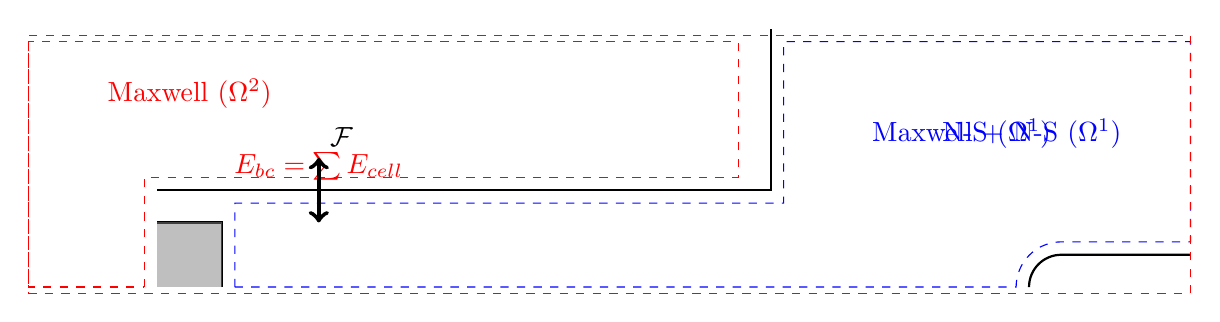
\begin{tikzpicture}[scale = .82]
			\draw[-, thick] (0, 0) -- (0,1) -- (-1.0,1);
			\fill[gray, opacity=0.5] (-1.0,0) -- (0, 0) -- (0,1) -- (-1.0,1) -- cycle;
			\draw[-,thick] (-1.0,1.5) -- (8.5,1.5) -- (8.5,4.);
			\draw[dashed, blue] (0.2, 0) -- (0.2, 1.3) -- (8.7, 1.3) -- (8.7, 3.8) -- (15, 3.8) -- (15, 0.7) -- (13, 0.7) arc[start angle=90, end angle = 180, radius=0.7] -- cycle;
			
			\onslide<1,3>
			{
			\draw[blue] (12,2) node[above]{Maxwell + N-S ($\Omega^1$)};
			}
			\onslide<2>
			{
			\draw[blue] (12,2) node[above]{N-S ($\Omega^1$)};
			}
			\draw[-, thick] (15, 0.5) -- (13,0.5) arc[start angle=90, end angle = 180, radius=0.5];
			
			\onslide<2->
			{
			\draw[red] (-0.5,3) node{Maxwell ($\Omega^2$)};
			}
			
			\onslide<2>
			{
			\draw[dashed, red] (-3.,-0.1) -- (15,-0.1) -- (15,3.9) -- (-3.,3.9) -- cycle;% (-1.2, 1.7) -- (8, 1.7) -- (8, 3.8) -- (-3, 3.8) -- (-3,0) -- cycle;
			}
			
			\onslide<1>
			{
			\node[red] at (1.5, 1.5) [above]{$E_{bc} = \sum E_{cell}$};
			%\draw[black, <->, ultra thick] (1.5,1) -- (1.5,2);
			}			
			
			\onslide<3>
			{
			\draw[dashed, red] (-1.2,0) -- (-1.2, 1.7) -- (8, 1.7) -- (8, 3.8) -- (-3, 3.8) -- (-3,0) -- cycle;
			\draw[black, <->, ultra thick] (1.5,1) -- (1.5,2) node[above right]{$\mathcal{F}$};
			}
			
			
		\end{tikzpicture}
\end{center}

\only<1>
{
Compact but fills the jacobian matrix, making it incompatible with HDG.
}

\only<2>
{
Most widely used. Solve N-S while Maxwell frozen, and \textit{vice versa}. Slow convergence.
}

\only<3>
{
Solves the system in a fully coupled manner, with two domains. The method we employ here.
}

\end{frame}

\begin{frame}{Modification of the model problem}

\begin{framed}
\begin{equation*}
	\begin{aligned}
		& \partial_t \vecw^l(\vecu) + \nabla \cdot \left(\vecF_c^l(\vecu) - \vecF_v^l(\vecu, \nabla \vecu)\right) = \vecS^l(\vecu, \nabla \vecu), && \text{ on } \Omega^l\\
		& \vecu^l = \vecu_{bc}^l, && \vecx\in\partial\Omega^l_d\\
		& \vecF_v^l \cdot \vecn = \vecF_{v,n,bc}^l, &&  \text{ on } \partial\Omega^l_n\\
		\only<1,3->
		{
		& \mathcal{F}^{l,l'}(\vecu^l, \nabla \vecu^l, \vecu^{l'}, \nabla \vecu^{l'}) = 0, &&  \text{ on }  \gamma^{l,l'}, \; l \neq l'\\
		}
		\only<2>
		{
		& \textcolor{red}{\mathcal{F}^{l,l'}(\vecu^l, \nabla \vecu^l, \vecu^{l'}, \nabla \vecu^{l'}) = 0}, &&  \text{ on }  \gamma^{l,l'}, \; l \neq l'\\
		}
		& \vecu^l(t = 0) = \vecU^l, &&  \text{ on }  \Omega^l
	\end{aligned}
\end{equation*}
\end{framed}

\onslide<3>
{
For ICP, 
\begin{equation*}
\mathcal{F} =
\begin{pmatrix}
\nabla E_p^{Re, NS} \cdot \vecn^{NS} - \nabla E_p^{Re, MAX} \cdot \vecn^{MAX}\\
\nabla E_p^{Im, NS} \cdot \vecn^{NS} - \nabla E_p^{Im, MAX} \cdot \vecn^{MAX}
\end{pmatrix}
\end{equation*}
}

\end{frame}

\begin{frame}{Modification of the discrete formulation}

\begin{framed}
\begin{equation*}
	\begin{aligned}
		& \left(\partial_t \vecw_h - \vecS_h^K, \varphi_{K,i} \right)_{K} - \left(\vecF_{h,c}^K - \vecF_{h,v}^K, \nabla \varphi_{K,i} \right)_{K} + \left\langle \vecHcal^K, \varphi_{K,i} \right\rangle_{\partial K} = 0\\
		& \left(\vecq_K, \vectau_{K,i}\right)_{K} - \left(\vecu_K, \nabla \vectau_{K',i}\right)_{K} + \left\langle \veclambda_{\partial K}, \vectau_{K,i} \cdot \vecn \right\rangle_{\partial K_0} + \left\langle \vecu_{bc}, \vectau_{K,i} \cdot \vecn \right\rangle_{\partial K_{bc}} = 0\\
		& \left\langle[[\vecHcal]], \mu_{e,i} \right\rangle_{e\setminus\Gammabar} \textcolor{red}{+ \langle \Tilde{\mathcal{F}^e}, \mu_{e,i}\rangle_{e\cap\Gammabar}} = 0\\
	\end{aligned}
\end{equation*}
\end{framed}

with $\bar{\Gamma}$ the set of interfaces between subdomains.

\end{frame}

\begin{frame}{Numerical fluxes : convection}

\begin{framed}
\begin{equation*}
\vecHcal = \vecHcal_c - \vecHcal_v
\end{equation*}
\end{framed}

\begin{equation*}
	\vecHcal_c = R \vecHcal_{c,n}(\vecu, \veclambda) = R (\dot{m} + \dot{m}_p) \Psi_\lambda - R |\dot{m}| (\Psi_\lambda - \Psi_U) + \vecP
\end{equation*}
with
\begin{equation*}
	\vecPsi = \begin{pmatrix} 1 & v^\perp & v^\parallel & v_\theta & e + \frac{1}{2} ||\mathbf{v}||^2 + \frac{p}{\rho} \end{pmatrix}^T
\end{equation*}
\begin{equation*}
\vecP = \begin{pmatrix} 0 & p_\lambda & 0 & 0 \end{pmatrix}^T
\end{equation*}


\end{frame}

\begin{frame}{Numerical fluxes : diffusion}

\begin{framed}
\begin{equation*}
\vecHcal = \vecHcal_c - \vecHcal_v
\end{equation*}
\end{framed}

\begin{equation*}
	\vecHcal_v(\vecu, \lambda, \vecq) = \vecF_v(\veclambda, \vecq) \cdot \mathbf{n} + \gamma(h) (\veclambda - \vecu)
\end{equation*}
with 
\begin{equation*}
	\gamma = C \max_{K \ni f}\left(\frac{1}{2\mathcal{V}} \sum_{f\in K} \mathcal{A}\right) 
\end{equation*}

C depends on the diffusive transport coefficients.

\end{frame}

\begin{frame}{Solution strategy}
The HDG system is solved at steady-state such that
\begin{equation*}
	\begin{aligned}
		\only<1>
		{
		& \left(\xcancel{\partial_t \vecw_h} - \vecS_h^K, \varphi_{K,i} \right)_{K} - \left(\vecF_{h,c}^K - \vecF_{h,v}^K, \nabla \varphi_{K,i} \right)_{K} + \left\langle \vecHcal^K, \varphi_{K,i} \right\rangle_{\partial K} = 0\\
		}
		\only<2->
		{
		& \left(\textcolor{red}{\frac{\delta\vecw_h^K}{\tau_{K,k}}} - \vecS_h^K, \varphi_{K,i} \right)_{K} - \left(\vecF_{h,c}^K - \vecF_{h,v}^K, \nabla \varphi_{K,i} \right)_{K} + \left\langle \vecHcal^K, \varphi_{K,i} \right\rangle_{\partial K} = 0\\
		}
		& \left(\vecq_K, \vectau_{K,i}\right)_{K} - \left(\vecu_K, \nabla \vectau_{K',i}\right)_{K} + \left\langle \veclambda_{\partial K}, \vectau_{K,i} \cdot \vecn \right\rangle_{\partial K_0} + \left\langle \vecu_{bc}, \vectau_{K,i} \cdot \vecn \right\rangle_{\partial K_{bc}} = 0\\
		& \left\langle[[\vecHcal]], \mu_{e,i} \right\rangle_{e\setminus\Gammabar} + \langle \Tilde{\mathcal{F}^e}, \mu_{e,i}\rangle_{e\cap\Gammabar} = 0\\
	\end{aligned}
\end{equation*}

\only<1>
{
If the system is written as $\mathcal{N} = 0$, then the Newton method solves
\begin{equation*}
\mathcal{N}'(\vecx_k) \delta \vecx_k = - \mathcal{N}(\vecx_k) 
\end{equation*}
with $\delta\vecx_k = \vecx_{k+1} - \vecx_k$.
}

\only<2>
{
If the system is written as $\tilde{\mathcal{N}} = 0$, then the Newton method solves
\begin{equation*}
\tilde{\mathcal{N}}'(\vecx_k) \delta \vecx = - \tilde{\mathcal{N}}(\vecx_k) 
\end{equation*}
with $\delta\vecx = \vecx_{k+1} - \vecx_k$.
}

\onslide<2->{

In order to stabilize the solver, a fictive temporal term is added.

}


\end{frame}

\begin{frame}{Damping term}

\begin{equation*}
\frac{\delta \vecw_h}{\tau_K} = \frac{\vecw(\vecu_{h,k+1}) - \vecw(\vecu_{h,k})}{\tau_{K,k}}
\end{equation*}
with
\begin{equation*}
\tau_{K,k} = CFL_k \frac{h_K}{v_K} = CFL_k \frac{V_K}{\int_{\partial K} \lambda_{max} dS}
\end{equation*}

and the following CFL evolution law
\begin{equation*}
CFL_k = \min\left(CFL_0 \left(\frac{||\mathcal{N}||_2^0}{||\mathcal{N}||_2^k}\right)^\alpha, CFL_{max}\right)
\end{equation*}

\onslide<2>
{
\begin{framed}
\centering
\textbf{We only use convective eigenvalues here. The diffusive could be use to enhance the convergence.}
\end{framed}
}

\end{frame}

\begin{frame}{Matrix form of the system}

\begin{framed}
\begin{equation*}
\tilde{\mathcal{N}}'(\vecx_k) \delta \vecx_k = - \tilde{\mathcal{N}}(\vecx_k) 
\end{equation*}
\end{framed}

\only<2>
{
\begin{equation*}
    \underbrace{
    \begin{pmatrix}
        A & B & R\\
        C & D & S\\
        L & M & N
    \end{pmatrix}
    }_{\Tilde{\mathcal{N}}'}
    \overbrace{
    \begin{pmatrix}
        \delta Q\\
        \delta U\\
        \delta \Lambda
    \end{pmatrix}
    }^{\delta \vecx}
    = 
    \underbrace{
    \begin{pmatrix}
        F\\
        G\\
        H
    \end{pmatrix}
    }_{-\Tilde{\mathcal{N}}},
\end{equation*}
}
\only<3>
{
The system can be split into two parts
\begin{equation*}
	\underbrace{
    \begin{pmatrix}
        A & B\\
        C & D
    \end{pmatrix}
    }_{\text{Block diagonal}}
    \begin{pmatrix}
        \delta Q\\
        \delta U\\
    \end{pmatrix}
    =
    \begin{pmatrix}
        F\\
        G
    \end{pmatrix}
    -
    \begin{pmatrix}
        R\\
        S
    \end{pmatrix}
    \delta \Lambda
\end{equation*}
and
\begin{equation*}
    \begin{pmatrix}
        L & M
    \end{pmatrix}
    \begin{pmatrix}
        \delta Q\\
        \delta U\\
    \end{pmatrix}
    + N \delta \Lambda
    = H
\end{equation*}
}

\only<4->
{
By eliminating $\delta U$ and $\delta Q$, one gets the \textbf{global} system
\begin{equation*}
    \begin{aligned}
    &\left(
    N -
    \begin{pmatrix}
        L & M
    \end{pmatrix}
    \begin{pmatrix}
        A & B\\
        C & D
    \end{pmatrix}^{-1}
    \begin{pmatrix}
        R\\
        S
    \end{pmatrix}
    \right)
    \delta \Lambda
    =
    H - 
    \begin{pmatrix}
        L & M
    \end{pmatrix}
    \begin{pmatrix}
        A & B\\
        C & D
    \end{pmatrix}^{-1}
    \begin{pmatrix}
        F\\
        G
    \end{pmatrix}
    \end{aligned}
\end{equation*}
}
\only<5>
{
This system is solved for $\veclambda$, then the \textbf{local} variables $\vecu$ and $\vecq$ are retrieved by inverting local small matrices.
\begin{equation*}
    \begin{pmatrix}
        \delta Q\\
        \delta U\\
    \end{pmatrix}
    =
    \begin{pmatrix}
        A & B\\
        C & D
    \end{pmatrix}^{-1}
    \begin{pmatrix}
        F\\
        G
    \end{pmatrix}
    -
    \begin{pmatrix}
        A & B\\
        C & D
    \end{pmatrix}^{-1}
    \begin{pmatrix}
        R\\
        S
    \end{pmatrix}
    \delta \Lambda
\end{equation*}
}
\end{frame}

\begin{frame}{The problem of power quenching.}

There is no straightforward relation linking the induction current and the power dissipated in the facility.

\textbf{If the power dissipated in the facility is not maintained during the simulation, the torch quenches!}

\begin{equation*}
	\begin{aligned}
		& \partial_t \rho + \nabla \cdot \left(\rho \vecv\right) =0\\
		& \partial_t \left(\rho \vecv\right) + \nabla \cdot \left(\rho \vecv \vecv\right) + \nabla p - \nabla \cdot \vectau = \gamma \left.\vecF^L\right|_{I_c = \SI{1}{\ampere}}\\
		& \partial_t \left(\rho e + \frac{1}{2} \rho ||\vecv||^2\right) + \nabla \cdot \left(\rho e \vecv + \frac{1}{2} \rho ||\vecv||^2 \vecv + p \vecv - \vectau \cdot \vecv - \vecq\right) = \gamma \left.P_J\right|_{I_c = \SI{1}{\ampere}}\\
	\end{aligned}
\end{equation*}

\begin{equation*}
	\Delta \left.E_P\right|_{I_c = \SI{1}{\ampere}} = \frac{\left.E_P\right|_{I_c = \SI{1}{\ampere}}}{r^2} + i 2 \pi f\mu_0\sigma_e \left(\left.E_C\right|_{I_c = \SI{1}{\ampere}} + \left.E_P\right|_{I_c = \SI{1}{\ampere}}\right)
\end{equation*}

\end{frame}

\begin{frame}{Power ratio}

At every Newton iteration, the induction current is set to $\SI{1}{\ampere}$. $\gamma$ is the power ratio
\begin{equation*}
\gamma = \frac{P_{target}}{P|_{I_c=\SI{1}{\ampere}}}
\end{equation*}
with $P_{target}$ the desired power and
\begin{equation*}
P|_{I_c=\SI{1}{\ampere}} = \int_{NS}\frac{\sigma_e}{2} ||\left.E_C\right|_{I_c = \SI{1}{\ampere}} + \left.E_P\right|_{I_c = \SI{1}{\ampere}}||^2 dV
\end{equation*}

$\gamma$ is computed at the beginning of every Newton iteration and used as a scaling factor for the Joule heating and Lorentz source terms evalutaed at $I_c = \SI{1}{\ampere}$. The true electric fields are given by
\begin{equation*}
E_C = \sqrt{\gamma} E_C|_{I_c = \SI{1}{\ampere}} \quad E_P = \sqrt{\gamma} E_P|_{I_c = \SI{1}{\ampere}}
\end{equation*}

\end{frame}

\section{Results}

\begin{frame}{Manufactured solution}

\begin{center}
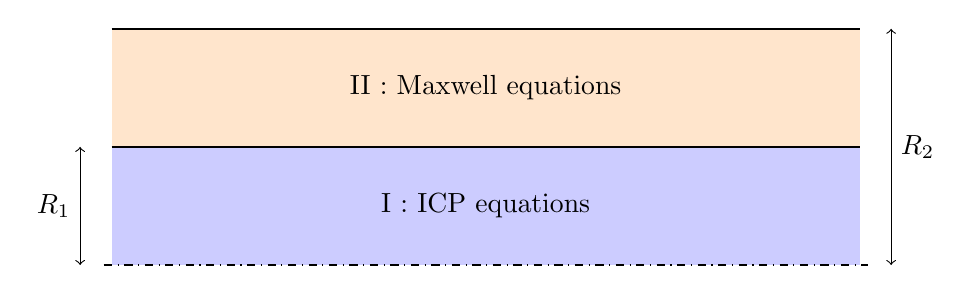
\begin{tikzpicture}
\fill[orange!20] (-1.0,1.5) -- (8.5,1.5) -- (8.5,3.) -- (-1.0,3.);
\fill[blue!20] (-1.0,1.5) -- (8.5,1.5) -- (8.5,0.) -- (-1.0, 0.);
\draw[dash dot, thick, black] (-1.1,0) -- (8.6,0);
\draw[-,thick, black] (-1.0,1.5) -- (8.5,1.5);
\draw[-,thick, black] (-1.0,3.) -- (8.5,3.);
\draw (3.75, 2.25) node{II : Maxwell equations};
\draw (3.75, .75) node{I : ICP equations};
\draw[<->] (8.9,0) -- (8.9,1.5) node[right] {$R_2$} -- (8.9, 3.);
\draw[<->] (-1.4,0) -- (-1.4,0.75) node[left] {$R_1$} -- (-1.4, 1.5);
\end{tikzpicture}
\end{center}

\begin{equation*}
\begin{aligned}
& p =\Delta p_{0} f(z,r) + p_{0} && T = T_{min} + \left(T_{max} - T_{min}\right) f(z,r)\\
& v_z = u_{0} f(z,r) && E_p = E_{0} f(z,r) (1 - i)\\
& v_r = u_{0} f(z,r) && v_\theta = u_{0} f(z,r) \\
\end{aligned}
\end{equation*}

with 
\begin{equation*}
f(z,r) = \left(\frac{rz}{RL}\right)^2\exp\left(-\frac{z}{L} - \frac{r}{R_1}\right)
\end{equation*}

\end{frame}

\begin{frame}{Convergence study : in the torch}
\centering
\begin{tabular}{cc}
\only<1>
{
\hspace{-1.3cm}% This file was created with tikzplotlib v0.10.1.
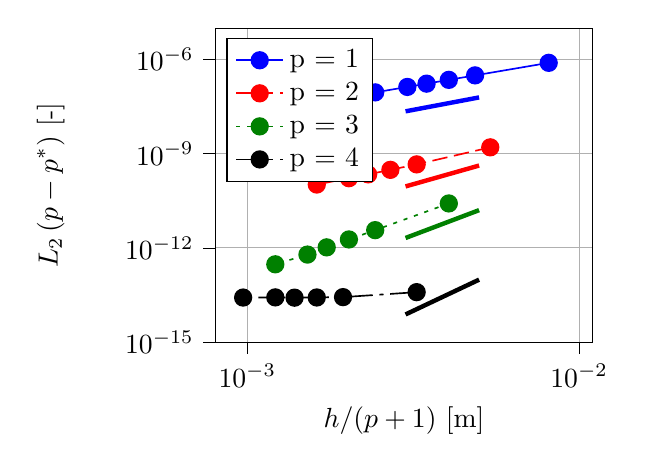
\begin{tikzpicture}

\definecolor{darkgray176}{RGB}{176,176,176}
\definecolor{darkturquoise0191191}{RGB}{0,191,191}
\definecolor{green}{RGB}{0,128,0}
\definecolor{lightgray204}{RGB}{204,204,204}

\begin{axis}[
scale = .7,
legend cell align={left},
legend pos = north west,
log basis x={10},
log basis y={10},
tick align=outside,
tick pos=left,
x grid style={darkgray176},
xmajorgrids,
xmin=0.0008, xmax=0.011,
xmode=log,
xlabel={\(\displaystyle h/(p+1)\) [m]},
xtick style={color=black},
xtick={0.0001,0.001,0.01,0.1,1},
xticklabels={
  \(\displaystyle {10^{-4}}\),
  \(\displaystyle {10^{-3}}\),
  \(\displaystyle {10^{-2}}\),
  \(\displaystyle {10^{-1}}\),
  \(\displaystyle {10^{0}}\)
},
%xlabel={\(\displaystyle \frac{h}{p+1}\) [m]},
y grid style={darkgray176},
ylabel={\(\displaystyle L_2\left(p - p^*\right)\) [-]},
ylabel style={yshift=15pt},
ymajorgrids,
ymin=1e-15, ymax=0.00001,
ymode=log,
ytick style={color=black},
%ytick={1e-13,1e-11,1e-9,1e-7,1e-5,1e-3},
%yticklabels={
%  \(\displaystyle {10^{-13}}\),
%  \(\displaystyle {10^{-11}}\),
%  \(\displaystyle {10^{-9}}\),
%  \(\displaystyle {10^{-7}}\),
%  \(\displaystyle {10^{-5}}\),
%  \(\displaystyle {10^{-3}}\)
%}
]
\addplot [semithick, blue, mark=*, mark size=3, mark options={solid}]
table {%
0.0081 7.90013e-07
0.00486 3.14639e-07
0.00405 2.26418e-07
0.00347142857142857 1.71405e-07
0.0030375 1.3474e-07
0.00243 9.03089e-08
};
\addlegendentry{p = 1}
\addplot [semithick, red, dash pattern=on 5.55pt off 2.4pt, mark=*, mark size=3, mark options={solid}]
table {%
0.0054 1.60139e-09
0.00324 4.58952e-10
0.0027 3.07117e-10
0.00231428571428571 2.20577e-10
0.002025 1.66428e-10
0.00162 1.0456e-10
};
\addlegendentry{p = 2}
\addplot [semithick, green, dash pattern=on 1.5pt off 2.475pt, mark=*, mark size=3, mark options={solid}]
table {%
0.00405 2.61297e-11
0.00243 3.68089e-12
0.002025 1.86166e-12
0.00173571428571429 1.04154e-12
0.00151875 6.13634e-13
0.001215 3.00462e-13
};
\addlegendentry{p = 3}
\addplot [semithick, black, dash pattern=on 9.6pt off 2.4pt on 1.5pt off 2.4pt, mark=*, mark size=3, mark options={solid}]
table {%
0.00324 3.8921e-14
0.001944 2.70126e-14
0.00162 2.63708e-14
0.00138857142857143 2.59766e-14
0.001215 2.65164e-14
0.000972 2.61729e-14
};
\addlegendentry{p = 4}

\addplot [domain=0.003:0.005, ultra thick, black] {((.5*x)^5)};
\addplot [domain=0.003:0.005, ultra thick, green] {((.4*x)^4)};
\addplot [domain=0.003:0.005, ultra thick, red] {((.15*x)^3)};
\addplot [domain=0.003:0.005, ultra thick, blue] {((.05*x)^2)};
\end{axis}

\end{tikzpicture}
 &
% This file was created with tikzplotlib v0.10.1.
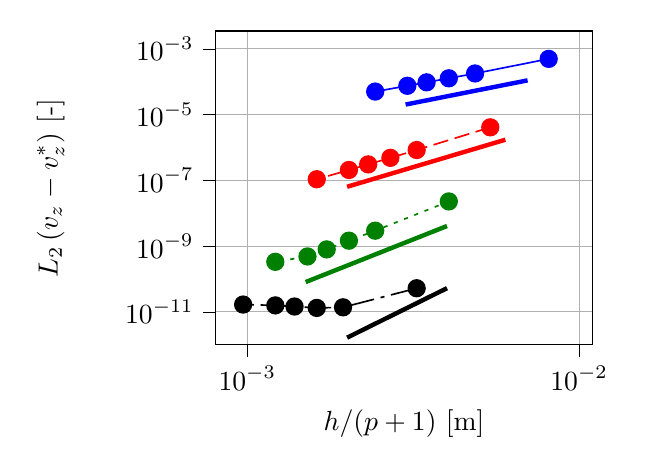
\begin{tikzpicture}

\definecolor{darkgray176}{RGB}{176,176,176}
\definecolor{darkturquoise0191191}{RGB}{0,191,191}
\definecolor{green}{RGB}{0,128,0}
\definecolor{lightgray204}{RGB}{204,204,204}

\begin{axis}[
scale = .7,
legend cell align={left},
legend style={
  fill opacity=0.8,
  draw opacity=1,
  text opacity=1,
  at={(0.03,0.97)},
  anchor=north west,
  draw=lightgray204
},
log basis x={10},
log basis y={10},
tick align=outside,
tick pos=left,
xlabel={\(\displaystyle h/(p+1)\) [m]},
x grid style={darkgray176},
xmajorgrids,
xmin=0.0008, xmax=0.011,
xmode=log,
xtick style={color=black},
xtick={0.0001,0.001,0.01,0.1,1},
xticklabels={
  \(\displaystyle {10^{-4}}\),
  \(\displaystyle {10^{-3}}\),
  \(\displaystyle {10^{-2}}\),
  \(\displaystyle {10^{-1}}\),
  \(\displaystyle {10^{0}}\)
},
%xlabel={\(\displaystyle \frac{h}{p+1}\) [m]},
y grid style={darkgray176},
ylabel={\(\displaystyle L_2\left(v_z - v_z^*\right)\) [-]},
ylabel style={yshift = 15pt},
ymajorgrids,
ymin=1e-12, ymax=0.0035,
ymode=log,
ytick style={color=black},
ytick={1e-13,1e-11,1e-9,1e-7,1e-5,1e-3},
yticklabels={
  \(\displaystyle {10^{-13}}\),
  \(\displaystyle {10^{-11}}\),
  \(\displaystyle {10^{-9}}\),
  \(\displaystyle {10^{-7}}\),
  \(\displaystyle {10^{-5}}\),
  \(\displaystyle {10^{-3}}\)
}
]
\addplot [semithick, blue, mark=*, mark size=3, mark options={solid}]
table {%
0.0081 0.000496167
0.00486 0.000178444
0.00405 0.000127146
0.00347142857142857 9.59307e-05
0.0030375 7.52771e-05
0.00243 5.01842e-05
};
%\addlegendentry{p = 1}
\addplot [semithick, red, dash pattern=on 5.55pt off 2.4pt, mark=*, mark size=3, mark options={solid}]
table {%
0.0054 4.10814e-06
0.00324 8.38197e-07
0.0027 4.84422e-07
0.00231428571428571 3.06634e-07
0.002025 2.07191e-07
0.00162 1.08552e-07
};
%\addlegendentry{p = 2}
\addplot [semithick, green, dash pattern=on 1.5pt off 2.475pt, mark=*, mark size=3, mark options={solid}]
table {%
0.00405 2.29148e-08
0.00243 2.95292e-09
0.002025 1.46668e-09
0.00173571428571429 7.96863e-10
0.00151875 4.85077e-10
0.001215 3.33773e-10
};
%\addlegendentry{p = 3}
\addplot [semithick, black, dash pattern=on 9.6pt off 2.4pt on 1.5pt off 2.4pt, mark=*, mark size=3, mark options={solid}]
table {%
0.00324 5.23855e-11
0.001944 1.38051e-11
0.00162 1.32185e-11
0.00138857142857143 1.45872e-11
0.001215 1.57807e-11
0.000972 1.67297e-11
};
%\addlegendentry{p = 4}
\addplot [domain=0.002:0.004, ultra thick, black] {((2.2*x)^5)};
\addplot [domain=0.0015:0.004, ultra thick, green] {((2*x)^4)};
\addplot [domain=0.002:0.006, ultra thick, red] {((2*x)^3)};
\addplot [domain=0.003:0.007, ultra thick, blue] {((1.5*x)^2)};

\end{axis}

\end{tikzpicture}

}
\only<2>
{
\hspace{-1.3cm}\input{./Convergence_Study_Plot_v_0} & % This file was created with tikzplotlib v0.10.1.
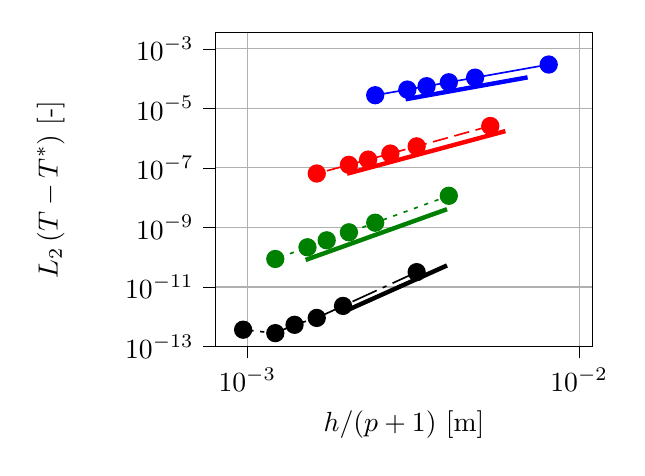
\begin{tikzpicture}

\definecolor{darkgray176}{RGB}{176,176,176}
\definecolor{darkturquoise0191191}{RGB}{0,191,191}
\definecolor{green}{RGB}{0,128,0}
\definecolor{lightgray204}{RGB}{204,204,204}

\begin{axis}[
scale = .7,
legend cell align={left},
legend style={
  fill opacity=0.8,
  draw opacity=1,
  text opacity=1,
  at={(0.03,0.97)},
  anchor=north west,
  draw=lightgray204
},
xlabel={\(\displaystyle h/(p+1)\) [m]},
log basis x={10},
log basis y={10},
tick align=outside,
tick pos=left,
x grid style={darkgray176},
xmajorgrids,
xmin=0.0008, xmax=0.011,
xmode=log,
xtick style={color=black},
xtick={0.0001,0.001,0.01,0.1,1},
xticklabels={
  \(\displaystyle {10^{-4}}\),
  \(\displaystyle {10^{-3}}\),
  \(\displaystyle {10^{-2}}\),
  \(\displaystyle {10^{-1}}\),
  \(\displaystyle {10^{0}}\)
},
%xlabel={\(\displaystyle \frac{h}{p+1}\) [m]},
y grid style={darkgray176},
ylabel={\(\displaystyle L_2\left(T - T^*\right)\) [-]},
ylabel style={yshift = 15pt},
ymajorgrids,
ymin=1e-13, ymax=0.0035,
ymode=log,
ytick style={color=black},
ytick={1e-13,1e-11,1e-9,1e-7,1e-5,1e-3},
yticklabels={
  \(\displaystyle {10^{-13}}\),
  \(\displaystyle {10^{-11}}\),
  \(\displaystyle {10^{-9}}\),
  \(\displaystyle {10^{-7}}\),
  \(\displaystyle {10^{-5}}\),
  \(\displaystyle {10^{-3}}\)
}
]
\addplot [semithick, blue, mark=*, mark size=3, mark options={solid}]
table {%
0.0081 0.00029749
0.00486 0.000107877
0.00405 7.53484e-05
0.00347142857142857 5.56664e-05
0.0030375 4.28383e-05
0.00243 2.76602e-05
};
%\addlegendentry{p = 1}
\addplot [semithick, red, dash pattern=on 5.55pt off 2.4pt, mark=*, mark size=3, mark options={solid}]
table {%
0.0054 2.56589e-06
0.00324 5.29582e-07
0.0027 3.03502e-07
0.00231428571428571 1.89983e-07
0.002025 1.26808e-07
0.00162 6.47224e-08
};
%\addlegendentry{p = 2}
\addplot [semithick, green, dash pattern=on 1.5pt off 2.475pt, mark=*, mark size=3, mark options={solid}]
table {%
0.00405 1.15592e-08
0.00243 1.43848e-09
0.002025 6.8637e-10
0.00173571428571429 3.69288e-10
0.00151875 2.15373e-10
0.001215 8.70897e-11
};
%\addlegendentry{p = 3}
\addplot [semithick, black, dash pattern=on 9.6pt off 2.4pt on 1.5pt off 2.4pt, mark=*, mark size=3, mark options={solid}]
table {%
0.00324 3.14979e-11
0.001944 2.30928e-12
0.00162 9.10392e-13
0.00138857142857143 5.3503e-13
0.001215 2.80798e-13
0.000972 3.66172e-13
};
%\addlegendentry{p = 4}

\addplot [domain=0.002:0.004, ultra thick, black] {((2.2*x)^5)};
\addplot [domain=0.0015:0.004, ultra thick, green] {((2*x)^4)};
\addplot [domain=0.002:0.006, ultra thick, red] {((2*x)^3)};
\addplot [domain=0.003:0.007, ultra thick, blue] {((1.5*x)^2)};

\end{axis}

\end{tikzpicture}

}
\end{tabular}
\only<3>
{
\begin{tabular}{c}
	% This file was created with tikzplotlib v0.10.1.
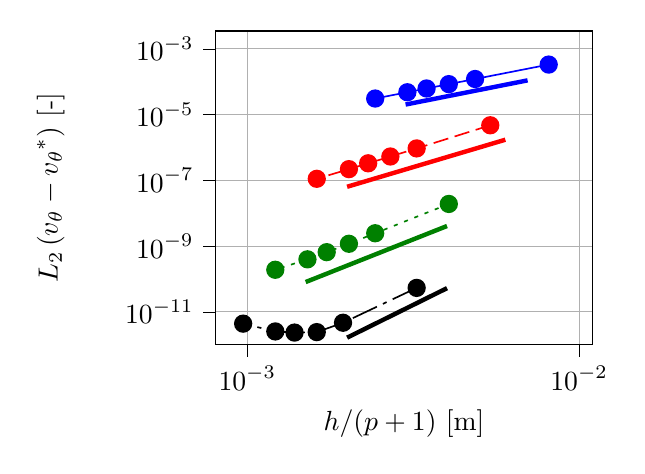
\begin{tikzpicture}

\definecolor{darkgray176}{RGB}{176,176,176}
\definecolor{green}{RGB}{0,128,0}
\definecolor{lightgray204}{RGB}{204,204,204}

\begin{axis}[
scale = .7,
legend cell align={left},
legend style={
  fill opacity=0.8,
  draw opacity=1,
  text opacity=1,
  at={(0.03,0.97)},
  anchor=north west,
  draw=lightgray204
},
log basis x={10},
log basis y={10},
tick align=outside,
tick pos=left,
x grid style={darkgray176},
xlabel={\(\displaystyle h/(p+1)\) [m]},
xmajorgrids,
xmin=0.0008, xmax=0.011,
xmode=log,
xtick style={color=black},
xtick={0.0001,0.001,0.01,0.1,1},
xticklabels={
  \(\displaystyle {10^{-4}}\),
  \(\displaystyle {10^{-3}}\),
  \(\displaystyle {10^{-2}}\),
  \(\displaystyle {10^{-1}}\),
  \(\displaystyle {10^{0}}\)
},
y grid style={darkgray176},
ylabel={\(\displaystyle L_2\left(v_\theta - {v_\theta}^*\right)\) [-]},
ylabel style={yshift = 15pt},
ymajorgrids,
ymin=1e-12, ymax=0.0035,
ymode=log,
ytick style={color=black},
ytick={1e-13,1e-11,1e-9,1e-7,1e-5,1e-3},
yticklabels={
  \(\displaystyle {10^{-13}}\),
  \(\displaystyle {10^{-11}}\),
  \(\displaystyle {10^{-9}}\),
  \(\displaystyle {10^{-7}}\),
  \(\displaystyle {10^{-5}}\),
  \(\displaystyle {10^{-3}}\)
}
]
\addplot [semithick, blue, mark=*, mark size=3, mark options={solid}]
table {%
0.0081 0.000332884
0.00486 0.000121155
0.00405 8.45613e-05
0.00347142857142857 6.23893e-05
0.0030375 4.79396e-05
0.00243 3.0865e-05
};
%\addlegendentry{p = 1}
\addplot [semithick, red, dash pattern=on 5.55pt off 2.4pt, mark=*, mark size=3, mark options={solid}]
table {%
0.0054 4.74088e-06
0.00324 9.37835e-07
0.0027 5.31781e-07
0.00231428571428571 3.30635e-07
0.002025 2.19761e-07
0.00162 1.11721e-07
};
%\addlegendentry{p = 2}
\addplot [semithick, green, dash pattern=on 1.5pt off 2.475pt, mark=*, mark size=3, mark options={solid}]
table {%
0.00405 1.91917e-08
0.00243 2.46703e-09
0.002025 1.18007e-09
0.00173571428571429 6.56445e-10
0.00151875 3.97685e-10
0.001215 1.91326e-10
};
%\addlegendentry{p = 3}
\addplot [semithick, black, dash pattern=on 9.6pt off 2.4pt on 1.5pt off 2.4pt, mark=*, mark size=3, mark options={solid}]
table {%
0.00324 5.3772e-11
0.001944 4.68163e-12
0.00162 2.43105e-12
0.00138857142857143 2.35266e-12
0.001215 2.54638e-12
0.000972 4.3986e-12
};
%\addlegendentry{p = 4}

\addplot [domain=0.002:0.004, ultra thick, black] {((2.2*x)^5)};
\addplot [domain=0.0015:0.004, ultra thick, green] {((2*x)^4)};
\addplot [domain=0.002:0.006, ultra thick, red] {((2*x)^3)};
\addplot [domain=0.003:0.007, ultra thick, blue] {((1.5*x)^2)};

\end{axis}

\end{tikzpicture}

\end{tabular}
}

\begin{framed}
\centering
\textbf{Convergence order of $p+1$ is retrieved!}
\end{framed}

\end{frame}

\begin{frame}{Convergence study : outside the torch}

\centering

\begin{tabular}{cc}
\only<1>
{
\hspace{-1.3cm}% This file was created with tikzplotlib v0.10.1.
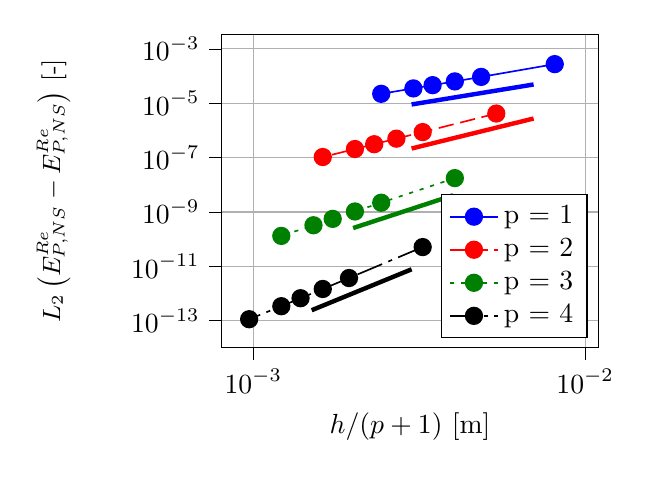
\begin{tikzpicture}

\definecolor{darkgray176}{RGB}{176,176,176}
\definecolor{darkturquoise0191191}{RGB}{0,191,191}
\definecolor{green}{RGB}{0,128,0}
\definecolor{lightgray204}{RGB}{204,204,204}

\begin{axis}[
scale = .7,
legend cell align={left},
legend pos=south east,
log basis x={10},
log basis y={10},
tick align=outside,
tick pos=left,
x grid style={darkgray176},
%xlabel={\(\displaystyle \frac{h}{p+1}\) [m]},
xmajorgrids,
xmin=0.0008, xmax=0.011,
xmode=log,
xlabel={\(\displaystyle h/(p+1)\) [m]},
xtick style={color=black},
xtick={0.0001,0.001,0.01,0.1,1},
xticklabels={
  \(\displaystyle {10^{-4}}\),
  \(\displaystyle {10^{-3}}\),
  \(\displaystyle {10^{-2}}\),
  \(\displaystyle {10^{-1}}\),
  \(\displaystyle {10^{0}}\)
},
y grid style={darkgray176},
ylabel={\small\(\displaystyle L_2\left(E_{P,NS}^{Re} - E_{P,NS}^{Re}\right)\) [-]},
ylabel style={yshift = 15pt},
ymajorgrids,
ymin=1e-14, ymax=0.0035,
ymode=log,
ytick style={color=black},
ytick={1e-13,1e-11,1e-9,1e-7,1e-5,1e-3},
yticklabels={
  \(\displaystyle {10^{-13}}\),
  \(\displaystyle {10^{-11}}\),
  \(\displaystyle {10^{-9}}\),
  \(\displaystyle {10^{-7}}\),
  \(\displaystyle {10^{-5}}\),
  \(\displaystyle {10^{-3}}\)
}
]
\addplot [semithick, blue, mark=*, mark size=3, mark options={solid}]
table {%
0.0081 0.000274153
0.00486 9.28418e-05
0.00405 6.35146e-05
0.00347142857142857 4.61742e-05
0.0030375 3.50762e-05
0.00243 2.2205e-05
};
\addlegendentry{p = 1}
\addplot [semithick, red, dash pattern=on 5.55pt off 2.4pt, mark=*, mark size=3, mark options={solid}]
table {%
0.0054 4.17292e-06
0.00324 8.67944e-07
0.0027 4.97005e-07
0.00231428571428571 3.10532e-07
0.002025 2.06772e-07
0.00162 1.04944e-07
};
\addlegendentry{p = 2}
\addplot [semithick, green, dash pattern=on 1.5pt off 2.475pt, mark=*, mark size=3, mark options={solid}]
table {%
0.00405 1.75844e-08
0.00243 2.18736e-09
0.002025 1.04218e-09
0.00173571428571429 5.57477e-10
0.00151875 3.24504e-10
0.001215 1.31583e-10
};
\addlegendentry{p = 3}
\addplot [semithick, black, dash pattern=on 9.6pt off 2.4pt on 1.5pt off 2.4pt, mark=*, mark size=3, mark options={solid}]
table {%
0.00324 5.11149e-11
0.001944 3.71707e-12
0.00162 1.46831e-12
0.00138857142857143 6.71249e-13
0.001215 3.41757e-13
0.000972 1.13372e-13
};
\addlegendentry{p = 4}


\addplot [domain=0.0015:0.003, ultra thick, black] {((2*x)^5)};
\addplot [domain=0.002:0.004, ultra thick, green] {((2*x)^4)};
\addplot [domain=0.003:0.007, ultra thick, red] {((2*x)^3)};
\addplot [domain=0.003:0.007, ultra thick, blue] {((1.*x)^2)};

\end{axis}

\end{tikzpicture}
 & % This file was created with tikzplotlib v0.10.1.
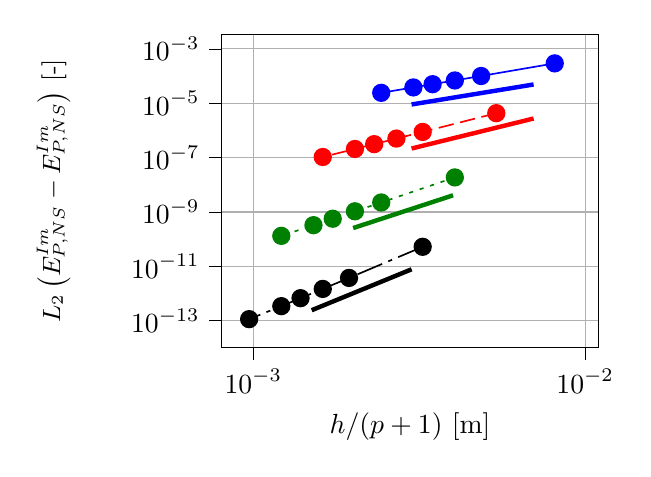
\begin{tikzpicture}

\definecolor{darkgray176}{RGB}{176,176,176}
\definecolor{darkturquoise0191191}{RGB}{0,191,191}
\definecolor{green}{RGB}{0,128,0}
\definecolor{lightgray204}{RGB}{204,204,204}

\begin{axis}[
scale = .7,
legend cell align={left},
legend style={
  fill opacity=0.8,
  draw opacity=1,
  text opacity=1,
  at={(0.03,0.97)},
  anchor=north west,
  draw=lightgray204
},
log basis x={10},
log basis y={10},
tick align=outside,
tick pos=left,
x grid style={darkgray176},
%xlabel={\(\displaystyle \frac{h}{p+1}\) [m]},
xmajorgrids,
xlabel={\(\displaystyle h/(p+1)\) [m]},
xmin=0.0008, xmax=0.011,
xmode=log,
xtick style={color=black},
xtick={0.0001,0.001,0.01,0.1,1},
xticklabels={
  \(\displaystyle {10^{-4}}\),
  \(\displaystyle {10^{-3}}\),
  \(\displaystyle {10^{-2}}\),
  \(\displaystyle {10^{-1}}\),
  \(\displaystyle {10^{0}}\)
},
y grid style={darkgray176},
ylabel={\small\(\displaystyle L_2\left(E_{P,NS}^{Im} - E_{P,NS}^{Im}\right)\) [-]},
ylabel style={yshift = 15pt},
ymajorgrids,
ymin=1e-14, ymax=0.0035,
ymode=log,
ytick style={color=black},
ytick={1e-13,1e-11,1e-9,1e-7,1e-5,1e-3},
yticklabels={
  \(\displaystyle {10^{-13}}\),
  \(\displaystyle {10^{-11}}\),
  \(\displaystyle {10^{-9}}\),
  \(\displaystyle {10^{-7}}\),
  \(\displaystyle {10^{-5}}\),
  \(\displaystyle {10^{-3}}\)
}
]
\addplot [semithick, blue, mark=*, mark size=3, mark options={solid}]
table {%
0.0081 0.000292529
0.00486 0.000100431
0.00405 6.88906e-05
0.00347142857142857 5.01501e-05
0.0030375 3.81208e-05
0.00243 2.41398e-05
};
%\addlegendentry{p = 1}
\addplot [semithick, red, dash pattern=on 5.55pt off 2.4pt, mark=*, mark size=3, mark options={solid}]
table {%
0.0054 4.3022e-06
0.00324 8.78014e-07
0.0027 5.00968e-07
0.00231428571428571 3.12325e-07
0.002025 2.07672e-07
0.00162 1.05228e-07
};
%\addlegendentry{p = 2}
\addplot [semithick, green, dash pattern=on 1.5pt off 2.475pt, mark=*, mark size=3, mark options={solid}]
table {%
0.00405 1.86545e-08
0.00243 2.23285e-09
0.002025 1.05704e-09
0.00173571428571429 5.63263e-10
0.00151875 3.27066e-10
0.001215 1.32242e-10
};
%\addlegendentry{p = 3}
\addplot [semithick, black, dash pattern=on 9.6pt off 2.4pt on 1.5pt off 2.4pt, mark=*, mark size=3, mark options={solid}]
table {%
0.00324 5.22806e-11
0.001944 3.74663e-12
0.00162 1.47635e-12
0.00138857142857143 6.73964e-13
0.001215 3.42876e-13
0.000972 1.14079e-13
};
%\addlegendentry{p = 4}

\addplot [domain=0.0015:0.003, ultra thick, black] {((2*x)^5)};
\addplot [domain=0.002:0.004, ultra thick, green] {((2*x)^4)};
\addplot [domain=0.003:0.007, ultra thick, red] {((2*x)^3)};
\addplot [domain=0.003:0.007, ultra thick, blue] {((1.*x)^2)};

\end{axis}

\end{tikzpicture}

}
\only<2>
{
\hspace{-1.5cm}% This file was created with tikzplotlib v0.10.1.
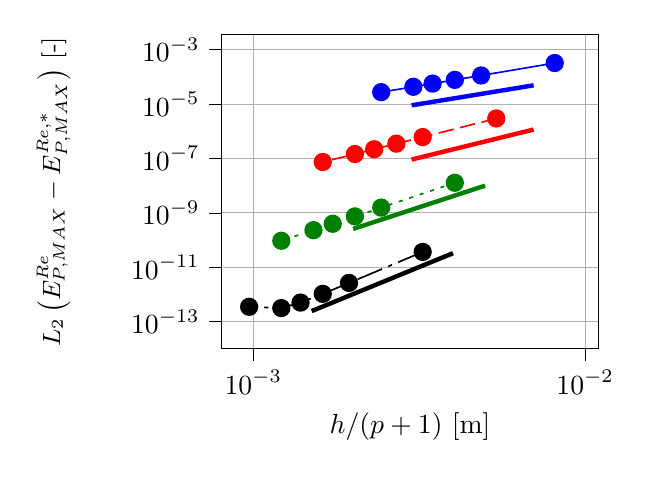
\begin{tikzpicture}

\definecolor{darkgray176}{RGB}{176,176,176}
\definecolor{darkturquoise0191191}{RGB}{0,191,191}
\definecolor{green}{RGB}{0,128,0}
\definecolor{lightgray204}{RGB}{204,204,204}

\begin{axis}[
scale = .7,
legend cell align={left},
legend style={
  fill opacity=0.8,
  draw opacity=1,
  text opacity=1,
  at={(0.03,0.97)},
  anchor=north west,
  draw=lightgray204
},
log basis x={10},
log basis y={10},
tick align=outside,
tick pos=left,
x grid style={darkgray176},
%xlabel={\(\displaystyle \frac{h}{p+1}\) [m]},
xmajorgrids,
xmin=0.0008, xmax=0.011,
xmode=log,
xtick style={color=black},
xtick={0.0001,0.001,0.01,0.1,1},
xticklabels={
  \(\displaystyle {10^{-4}}\),
  \(\displaystyle {10^{-3}}\),
  \(\displaystyle {10^{-2}}\),
  \(\displaystyle {10^{-1}}\),
  \(\displaystyle {10^{0}}\)
},
xlabel={\(\displaystyle h/(p+1)\) [m]},
y grid style={darkgray176},
ylabel={\small\(\displaystyle L_2\left(E_{P,MAX}^{Re} - {E_{P,MAX}^{Re,*}}\right)\) [-]},
ylabel style={yshift = 15pt},
ymajorgrids,
ymin=1e-14, ymax=0.0035,
ymode=log,
ytick style={color=black},
ytick={1e-13,1e-11,1e-9,1e-7,1e-5,1e-3},
yticklabels={
  \(\displaystyle {10^{-13}}\),
  \(\displaystyle {10^{-11}}\),
  \(\displaystyle {10^{-9}}\),
  \(\displaystyle {10^{-7}}\),
  \(\displaystyle {10^{-5}}\),
  \(\displaystyle {10^{-3}}\)
}
]
\addplot [semithick, blue, mark=*, mark size=3, mark options={solid}]
table {%
0.0081 0.0003235
0.00486 0.000112711
0.00405 7.76258e-05
0.00347142857142857 5.66932e-05
0.0030375 4.3212e-05
0.00243 2.74825e-05
};
%\addlegendentry{p = 1}
\addplot [semithick, red, dash pattern=on 5.55pt off 2.4pt, mark=*, mark size=3, mark options={solid}]
table {%
0.0054 2.95618e-06
0.00324 6.1082e-07
0.0027 3.49599e-07
0.00231428571428571 2.18427e-07
0.002025 1.45468e-07
0.00162 7.38667e-08
};
%\addlegendentry{p = 2}
\addplot [semithick, green, dash pattern=on 1.5pt off 2.475pt, mark=*, mark size=3, mark options={solid}]
table {%
0.00405 1.27121e-08
0.00243 1.55491e-09
0.002025 7.39167e-10
0.00173571428571429 3.94928e-10
0.00151875 2.29748e-10
0.001215 9.35466e-11
};
%\addlegendentry{p = 3}
\addplot [semithick, black, dash pattern=on 9.6pt off 2.4pt on 1.5pt off 2.4pt, mark=*, mark size=3, mark options={solid}]
table {%
0.00324 3.64334e-11
0.001944 2.63706e-12
0.00162 1.04529e-12
0.00138857142857143 4.99314e-13
0.001215 3.12953e-13
0.000972 3.49126e-13
};
%\addlegendentry{p = 4}


\addplot [domain=0.0015:0.004, ultra thick, black] {((2*x)^5)};
\addplot [domain=0.002:0.005, ultra thick, green] {((2*x)^4)};
\addplot [domain=0.003:0.007, ultra thick, red] {((1.5*x)^3)};
\addplot [domain=0.003:0.007, ultra thick, blue] {((1.*x)^2)};

\end{axis}

\end{tikzpicture}
 & \input{./Convergence_Study_Plot_EpIm_1}
}
\end{tabular}

\begin{framed}
\centering
\textbf{Convergence order of $p+1$ is retrieved!}
\end{framed}

\end{frame}

\begin{frame}{Grid and order dependence study}

\begin{figure}[h]
	\centering
	\includegraphics[width=\linewidth]{./Grid_Independence_mesh_probe_cropped.pdf}
	\reflectbox{\includegraphics[width = \linewidth, angle=180, origin=c]{./ConvergenceFS_coarse-crop.pdf}}
\end{figure} 

\only<1>
{
\begin{framed}
\centering
\textbf{Mesh independence study : this relatively coarse mesh at $p=4$ with 4013 elements for the probe case and 3055 for the freestream case.}
\end{framed}

In the following we only consider the probe case.

}

\only<2>
{
The mesh size close to the probe is $\SI{10}{\micro\meter}$ thick, while it is of $\SI{1}{\micro\meter}$ for the finite volume solvers!
}

\end{frame}

\begin{frame}{The question of the coflow}

\begin{framed}
\textbf{A coflow is introduced in the chamber for obtaining a steady state, does it have an important impact?}
\only<5>{\textcolor{red}{Short answer is no.}}
\end{framed}

\only<2>
{
We consider an ICP flow with the following characteristics
\begin{itemize}
	\item $P = \SI{100}{\kilo\watt}$ (power dissipated in the facility)
	\item $p_0 = \SI{10000}{\pascal}$ (background pressure)
	\item $f = \SI{0.37}{\mega\hertz}$ (induction frequency)
	\item $Q = \SI{16}{\gram\;\second^{-1}}$ (mass flow rate)
	\item $S = \SI{20}{\degree}$ (swirl angle)
	\item air mixture with 11 species
\end{itemize}
}
\only<3>
{
\centering
	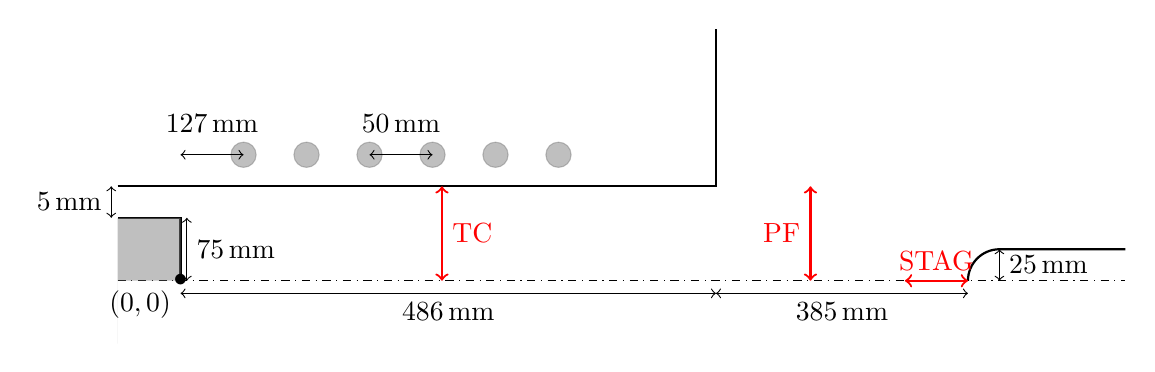
\begin{tikzpicture}[scale = .8]
		\draw[dash dot] (-1.0,0) -- (15,0);
		\draw[-, thick] (0, 0) -- (0,1) -- (-1.0,1);
		\fill[gray, opacity=0.5] (-1.0,0) -- (0, 0) -- (0,1) -- (-1.0,1) -- (-1.0,-1);
		\draw[-,thick] (-1.0,1.5) -- (8.5,1.5) -- (8.5,4.);
		\foreach \x in {1,2,...,6}{
			\filldraw[gray, opacity = 0.5] (\x, 2.) circle (0.2);
		}
		\draw[-, thick] (15, 0.5) -- (13,0.5) arc[start angle=90, end angle = 180, radius=0.5];
		\draw[<->] (0,2) -- (1.,2);
		\draw (.5,2.5) node{$\SI{127}{\milli\meter}$};
		\draw[<->] (3,2) -- (4,2);
		\draw (3.5,2.5) node{$\SI{50}{\milli\meter}$};
		\draw[<->] (0,-0.2) -- node[below]{$\SI{486}{\milli\meter}$} (8.5,-0.2);
		\draw[<->] (8.5,-0.2) -- node[below]{$\SI{385}{\milli\meter}$} (12.5,-0.2);
		\draw[<->] (0.1,0) -- node[right]{$\SI{75}{\milli\meter}$} (0.1,1);
		\draw[<->] (-1.1, 1.) -- node[left]{$\SI{5}{\milli\meter}$} (-1.1,1.5);
		\draw[<->] (13,0) -- node[right]{$\SI{25}{\milli\meter}$} (13,0.5);
		\draw[thick, red, <->] (12.5, 0.) -- (12, 0.) node[above]{STAG} -- (11.5, 0.);
		\draw[thick, red, <->] (4.15, 0.) -- (4.15, 0.75) node[right]{TC} -- (4.15, 1.5);
		\draw[thick, red, <->] (10, 0.) -- (10, 0.75) node[left]{PF} -- (10, 1.5);
		\draw[black] (0,0) node{$\bullet$};
		\draw[black] (0,0) node[below left]{$(0,0)$};  
	\end{tikzpicture}
}

\only<4>
{
The coflow parameter $\chi$ is defined as
\begin{equation*}
\chi = \frac{U_{blow}}{U_{in}}
\end{equation*}
and tested from $0.2$ to $1.0$.
}

\only<5>
{
%Short answer, $\chi$ does not have an impact, the only measurable impact being on the region where the coflow is injected.
\begin{tabular}{cc}
% This file was created with tikzplotlib v0.10.1.
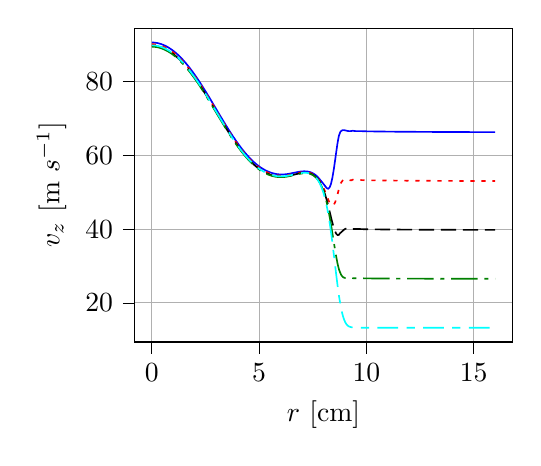
\begin{tikzpicture}

\definecolor{aqua}{RGB}{0,255,255}
\definecolor{darkgray176}{RGB}{176,176,176}
\definecolor{green}{RGB}{0,128,0}

\begin{axis}[
scale = .7,
ylabel = {$v_z$ [m $s^{-1}$]},
legend cell align=left,
xlabel = {$r$ [cm]},
legend pos=south west,
tick align=outside,
tick pos=left,
x grid style={darkgray176},
xmajorgrids,
xmin=-0.799999982118607, xmax=16.7999996244907,
xtick style={color=black},
y grid style={darkgray176},
ymajorgrids,
ymin=9.36328202198831, ymax=94.4853025712524,
ytick style={color=black}
]
\addplot [semithick, blue]
table {%
	0 90.6161198190131
	0.015999999595806 90.6151612211619
	0.031999999191612 90.613515180772
	0.047999998787418 90.6106351465569
	0.063999998383224 90.6063903051662
	0.07999999797903 90.6014636202648
	0.095999997574836 90.5947782444858
	0.112000002991408 90.5872764420772
	0.127999996766448 90.5786962560359
	0.14400000218302 90.5686224673639
	0.15999999595806 90.5578695630601
	0.176000001374632 90.5454927714122
	0.191999995149672 90.5321536512671
	0.208000000566244 90.5178627494233
	0.224000005982816 90.5019139646313
	0.239999988116324 90.4852702422664
	0.255999993532896 90.4670998480757
	0.271999998949468 90.4478967200847
	0.28800000436604 90.4278675189709
	0.303999986499548 90.4060763724585
	0.31999999191612 90.3836326318736
	0.335999997332692 90.3597308613845
	0.352000002749264 90.3347100351632
	0.367999984882772 90.3088405046578
	0.383999990299344 90.2812199626243
	0.399999972432852 90.2529521620591
	0.416000001132488 90.2232450170273
	0.431999983265996 90.1924176520654
	0.448000011965632 90.1607853838324
	0.46399999409914 90.127395090409
	0.479999976232648 90.0933545555365
	0.496000004932284 90.0578718690285
	0.511999987065792 90.0212549361819
	0.5279999691993 89.9838281300872
	0.543999997898936 89.9446820711912
	0.559999980032444 89.9048937516893
	0.57600000873208 89.8636375648858
	0.591999990865588 89.8213071752279
	0.607999972999096 89.7781122190742
	0.624000001698732 89.7332454367282
	0.63999998383224 89.6877530649079
	0.655999965965748 89.6407150532199
	0.671999994665384 89.5926927336107
	0.687999976798892 89.5437210309916
	0.704000005498528 89.4931729436665
	0.719999987632036 89.4420007114035
	0.735999969765544 89.3891989221721
	0.75199999846518 89.3355070394808
	0.767999980598688 89.280776491834
	0.784000009298325 89.2245525291296
	0.799999944865704 89.1676779213233
	0.81599997356534 89.1091136569026
	0.832000002264977 89.0497290113599
	0.847999937832355 88.9892761965285
	0.863999966531992 88.9273983975984
	0.879999995231628 88.8648662526561
	0.896000023931265 88.8006913626618
	0.911999959498644 88.7356743194942
	0.92799998819828 88.6696162990719
	0.944000016897917 88.6021210436814
	0.959999952465296 88.5339756171835
	0.975999981164932 88.4642198876191
	0.992000009864569 88.3936112250697
	1.00799994543195 88.3219875661819
	1.02399997413158 88.2489306574472
	1.04000000283122 88.1752315747746
	1.0559999383986 88.099911557151
	1.07199996709824 88.0237558766403
	1.08799999579787 87.9466441256908
	1.10399993136525 87.8680305340097
	1.11999996006489 87.788639457416
	1.13599998876452 87.7081606046799
	1.15200001746416 87.6263514097155
	1.16799995303154 87.5437689871305
	1.18399998173118 87.4599405457366
	1.20000001043081 87.374956369743
	1.21599994599819 87.2892039672665
	1.23199997469783 87.2020529834087
	1.24800000339746 87.1139225107041
	1.26399993896484 87.0250272284322
	1.27999996766448 86.9345205349931
	1.29599999636412 86.8432117357454
	1.3119999319315 86.751039735989
	1.32799996063113 86.657278003548
	1.34399998933077 86.5632400561772
	1.35999992489815 86.4675575636837
	1.37599995359778 86.3711554085126
	1.39199998229742 86.2736077865984
	1.40800001099706 86.1752171519126
	1.42399994656444 86.0754863602143
	1.43999997526407 85.9749310403448
	1.45600000396371 85.8734252798707
	1.47199993953109 85.7708640503859
	1.48799996823072 85.6671930915717
	1.50399999693036 85.562515631505
	1.51999993249774 85.4570814123172
	1.53599996119738 85.350556307347
	1.55199998989701 85.2430367516788
	1.56800001859665 85.1342841352434
	1.58399995416403 85.0249645794385
	1.59999988973141 84.9143810284728
	1.6160000115633 84.8033263754113
	1.63199994713068 84.6906652040595
	1.64799988269806 84.5776649702923
	1.66400000452995 84.4631785090891
	1.67999994009733 84.3482205706654
	1.69599987566471 84.2320202826704
	1.7119999974966 84.1151390194014
	1.72799993306398 83.9972423293153
	1.74399986863136 83.8784763363033
	1.75999999046326 83.758901024442
	1.77599992603064 83.6382848519555
	1.79200004786253 83.5170519457749
	1.80799998342991 83.3946218955557
	1.82399991899729 83.2717531329199
	1.84000004082918 83.1475442640586
	1.85599997639656 83.0230591149457
	1.87199991196394 82.8971112839907
	1.88800003379583 82.7710299551512
	1.90399996936321 82.6433014079452
	1.91999990493059 82.5154559790809
	1.93600002676249 82.3861823771277
	1.95199996232986 82.2566821490797
	1.96799989789724 82.12600818713
	1.98400001972914 81.9950191087692
	1.99999995529652 81.8627423656569
	2.0159998908639 81.7302158791078
	2.03200001269579 81.5964706505346
	2.04799994826317 81.4623884079392
	2.06399988383055 81.3272721842526
	2.08000000566244 81.1916737997202
	2.09599994122982 81.0552214693311
	2.1119998767972 80.9181515773847
	2.12799999862909 80.7803981135183
	2.14399993419647 80.641878175653
	2.15999986976385 80.5028196956941
	2.17599999159575 80.3628879907683
	2.19199992716312 80.2226103791188
	2.2079998627305 80.0813414488894
	2.2239999845624 79.939827970411
	2.23999992012978 79.7973162333584
	2.25600004196167 79.6544951553545
	2.27199997752905 79.5108614504142
	2.28799991309643 79.3668783844215
	2.30400003492832 79.2221817432228
	2.3199999704957 79.0770048299573
	2.33599990606308 78.9312872556536
	2.35200002789497 78.7849671544733
	2.36799996346235 78.6382664689098
	2.38399989902973 78.4908595626699
	2.40000002086163 78.3432141686134
	2.415999956429 78.1947721746227
	2.43199989199638 78.046226239816
	2.44800001382828 77.8968012711706
	2.46399994939566 77.7473096956785
	2.47999988496304 77.5970437586898
	2.49600000679493 77.4466291424985
	2.51199994236231 77.2955804650346
	2.52799987792969 77.144304864999
	2.54399999976158 76.9925223554342
	2.55999993532896 76.8404035075611
	2.57599987089634 76.68791460325
	2.59199999272823 76.5351904968517
	2.60799992829561 76.3819941646416
	2.62399986386299 76.2286476770139
	2.63999998569489 76.0747975013513
	2.65599992126226 75.9208755739219
	2.67199985682964 75.7664310072096
	2.68799997866154 75.6119802799861
	2.70399991422892 75.4569942888463
	2.7199998497963 75.302062446933
	2.73599997162819 75.1465912434905
	2.75199990719557 74.9912221196741
	2.76800002902746 74.8353402168637
	2.78399996459484 74.6795459454246
	2.79999990016222 74.52334899428
	2.81600002199411 74.3671859162466
	2.83199995756149 74.2107204290387
	2.84799989312887 74.0542509204979
	2.86400001496077 73.8975634588413
	2.87999995052814 73.7408450320799
	2.89599988609552 73.584011972162
	2.91200000792742 73.4270928666972
	2.9279999434948 73.2701502821799
	2.94399987906218 73.1131053029415
	2.96000000089407 72.9560810446458
	2.97599993646145 72.7989918614582
	2.99199987202883 72.6419186880416
	3.00799999386072 72.4848544864373
	3.0239999294281 72.3278052446785
	3.03999986499548 72.1707925583507
	3.05599998682737 72.0138421144545
	3.07199992239475 71.8569145252246
	3.08799985796213 71.7001329746221
	3.10399997979403 71.5433794350106
	3.1199999153614 71.3867759193591
	3.1360000371933 71.2302737162333
	3.15199978649616 71.0738769224802
	3.16799990832806 70.9177010889198
	3.18400003015995 70.7615442815148
	3.19999977946281 70.6057621507569
	3.21599990129471 70.4500053927438
	3.2320000231266 70.2945561472119
	3.24799977242947 70.1392771104126
	3.26399989426136 69.984231319047
	3.28000001609325 69.8295424969804
	3.29599976539612 69.6747875892655
	3.31199988722801 69.5206861354287
	3.32800000905991 69.3666062140244
	3.34399975836277 69.212810272551
	3.35999988019466 69.0595174259175
	3.37600000202656 68.906167081888
	3.39199975132942 68.7536274479068
	3.40799987316132 68.6011494285524
	3.42399999499321 68.4490163258322
	3.43999974429607 68.2974937728385
	3.45599986612797 68.1459211348559
	3.47199998795986 67.9952783059475
	3.48799973726273 67.8447452977844
	3.50399985909462 67.6945874105809
	3.51999998092651 67.5451500119556
	3.53600010275841 67.3956785771587
	3.55199985206127 67.24723135712
	3.56799997389317 67.0989603899184
	3.58400009572506 66.9510732550211
	3.59999984502792 66.8040825777045
	3.61599996685982 66.6570650498841
	3.63200008869171 66.5111155400106
	3.64799983799458 66.3654582325617
	3.66399995982647 66.2201294902035
	3.68000008165836 66.0758600026337
	3.69599983096123 65.9315825334035
	3.71199995279312 65.7884959997043
	3.72800007462502 65.6456372399658
	3.74399982392788 65.5034099223217
	3.75999994575977 65.3620446239706
	3.77600006759167 65.2206859245761
	3.79199981689453 65.0808842109807
	3.80799993872643 64.9410818494004
	3.82400006055832 64.8022290337085
	3.83999980986118 64.6640595132493
	3.85599993169308 64.5261602111731
	3.87200005352497 64.3896803173657
	3.88799980282784 64.2532160092762
	3.90399992465973 64.1180216781804
	3.92000004649162 63.9833136599905
	3.93599979579449 63.8491521683409
	3.95199991762638 63.7162732307699
	3.96800003945827 63.5834193661317
	3.98399978876114 63.4521544798963
	3.99999991059303 63.3211853153472
	4.01600003242493 63.1910096124371
	4.03199978172779 63.0619822673008
	4.04799990355968 62.9329886698989
	4.06400002539158 62.8057686128462
	4.07999977469444 62.6788161843459
	4.09599989652634 62.5528665937488
	4.11200001835823 62.4279097903601
	4.12799976766109 62.3032872714867
	4.14399988949299 62.1806285923227
	4.16000001132488 62.0579529137978
	4.17599976062775 61.9358347606759
	4.19199988245964 61.8155674770203
	4.20800000429153 61.6956311825817
	4.2239997535944 61.5765761438538
	4.23999987542629 61.458589584868
	4.25599999725819 61.3414715313022
	4.27199974656105 61.2255724782269
	4.28799986839294 61.1104413804487
	4.30399999022484 60.9956706006252
	4.3199997395277 60.8830155763147
	4.3359998613596 60.7708167947748
	4.35199998319149 60.6585541793847
	4.36799973249435 60.5488806897387
	4.38399985432625 60.4395454537213
	4.39999997615814 60.3304030824542
	4.41599972546101 60.2233129068076
	4.4319998472929 60.1170474742428
	4.44799996912479 60.011312133891
	4.46399971842766 59.9071294736245
	4.47999984025955 59.8035601148199
	4.49599996209145 59.7012580731739
	4.51200008392334 59.6003286863369
	4.5279998332262 59.4997177064415
	4.5439999550581 59.3998495657344
	4.56000007688999 59.3021934600577
	4.57599982619286 59.2050097715323
	4.59199994802475 59.1081650788471
	4.60800006985664 59.0136727135973
	4.62399981915951 58.9196104209932
	4.6399999409914 58.8260169703416
	4.6560000628233 58.7344766264735
	4.67199981212616 58.6439336770371
	4.68799993395805 58.5537588603065
	4.70400005578995 58.4647670846827
	4.71999980509281 58.3775367597549
	4.73599992692471 58.2909361928242
	4.7520000487566 58.20485980783
	4.76799979805946 58.1210442302914
	4.78399991989136 58.0376192453131
	4.80000004172325 57.9553041290561
	4.81599979102612 57.8741235816061
	4.83199991285801 57.794449524529
	4.8480000346899 57.7153027937569
	4.86399978399277 57.637203738075
	4.87999990582466 57.5601652069194
	4.89600002765656 57.4848993890305
	4.91199977695942 57.4103320202692
	4.92799989879131 57.3365538736477
	4.94400002062321 57.2640447070449
	4.95999976992607 57.1929761994791
	4.97599989175797 57.1229013047163
	4.99200001358986 57.0534449823761
	5.00799976289272 56.9853677565093
	5.02399988472462 56.9186697786957
	5.04000000655651 56.8529684867157
	5.05599975585938 56.7877901231303
	5.07199987769127 56.7240158894226
	5.08799999952316 56.6614219618478
	5.10399974882603 56.5993886772283
	5.11999987065792 56.5395678069198
	5.13599999248981 56.4798137992984
	5.15199974179268 56.4218362708712
	5.16799986362457 56.3653532108276
	5.18399998545647 56.3086970890899
	5.19999973475933 56.2536925716678
	5.21599985659122 56.200184166562
	5.23199997842312 56.1470626491645
	5.24799972772598 56.0957529703185
	5.26399984955788 56.0444420968072
	5.27999997138977 55.9950639099919
	5.29599972069263 55.9464998933136
	5.31199984252453 55.8978670425404
	5.32799996435642 55.8518837309056
	5.34399971365929 55.8076278674763
	5.35999983549118 55.7639629137077
	5.37599995732307 55.7212569837422
	5.39199970662594 55.6791908888309
	5.40799982845783 55.6375040589873
	5.42399995028973 55.5968313321429
	5.43999969959259 55.5576464928122
	5.45599982142448 55.5188641396063
	5.47199994325638 55.4804788841991
	5.48799969255924 55.4442318028621
	5.50399981439114 55.4087398942379
	5.51999993622303 55.3739936016224
	5.53600005805492 55.3404448581298
	5.55199980735779 55.3087492266043
	5.56799992918968 55.2774490861125
	5.58400005102158 55.2465819684587
	5.59999980032444 55.2180993854846
	5.61599992215633 55.1906398897422
	5.63200004398823 55.1635053575998
	5.64799979329109 55.136691732261
	5.66399991512299 55.1120338767194
	5.68000003695488 55.0882139297669
	5.69599978625774 55.064747147398
	5.71199990808964 55.0415484007964
	5.72800002992153 55.0206581948979
	5.7439997792244 55.0000442811096
	5.75999990105629 54.9799335050735
	5.77600002288818 54.9603729835544
	5.79199977219105 54.9437526586104
	5.80799989402294 54.9276250748998
	5.82400001585484 54.9119523542838
	5.8399997651577 54.8956848392564
	5.85599988698959 54.8849453149931
	5.87200000882149 54.8755907999842
	5.88799975812435 54.8668472444525
	5.90399987995625 54.8587172283387
	5.92000000178814 54.8505403437556
	5.935999751091 54.8418112745098
	5.9519998729229 54.8338852239917
	5.96799999475479 54.8265999916312
	5.98399974405766 54.8209868870209
	5.99999986588955 54.8171526683588
	6.01599998772144 54.8143896695287
	6.03199973702431 54.8122834532786
	6.0479998588562 54.8113477997157
	6.0639999806881 54.8118824877274
	6.07999972999096 54.8128258951195
	6.09599985182285 54.8148911475747
	6.11199997365475 54.8177961341084
	6.12799972295761 54.8221392915664
	6.14399984478951 54.8268593131321
	6.1599999666214 54.8320289239203
	6.17599971592426 54.838354186478
	6.19199983775616 54.8462940641859
	6.20799995958805 54.8545988335355
	6.22399970889091 54.8632662754936
	6.23999983072281 54.8724584435972
	6.2559999525547 54.8836370629789
	6.2720000743866 54.8953394860551
	6.28800019621849 54.9073707604316
	6.30399957299232 54.9197285102606
	6.31999969482422 54.9332601511938
	6.33599981665611 54.9479264436426
	6.35199993848801 54.9628493658689
	6.3680000603199 54.978027531781
	6.38400018215179 54.9936257418397
	6.39999955892563 55.010347229415
	6.41599968075752 55.0274382301315
	6.43199980258942 55.0446982472106
	6.44799992442131 55.0621263782404
	6.4640000462532 55.0801157756194
	6.4800001680851 55.0985204899558
	6.49599954485893 55.1171287721448
	6.51199966669083 55.1358491398574
	6.52799978852272 55.1547533910202
	6.54399991035461 55.1739908240935
	6.56000003218651 55.1934341053805
	6.5760001540184 55.2130010910284
	6.59199953079224 55.2326639023591
	6.60799965262413 55.2525103601803
	6.62399977445602 55.2724661776442
	6.63999989628792 55.2921841258712
	6.65600001811981 55.3118717732124
	6.67200013995171 55.3315283557928
	6.68799951672554 55.3510727525414
	6.70399963855743 55.3703452741083
	6.71999976038933 55.3892735152027
	6.73599988222122 55.4080560759958
	6.75200000405312 55.4266016844966
	6.76800012588501 55.444805020015
	6.78399950265884 55.4624452496753
	6.79999962449074 55.4797069486552
	6.81599974632263 55.4967481243783
	6.83199986815453 55.5132675471045
	6.84799998998642 55.5293147910108
	6.86400011181831 55.5443372835759
	6.87999948859215 55.5589602333563
	6.89599961042404 55.5732533409249
	6.91199973225594 55.5865800989818
	6.92799985408783 55.5992183978762
	6.94399997591972 55.6104089469256
	6.96000009775162 55.6211380566331
	6.97599947452545 55.6314092989785
	6.99199959635735 55.6402371365635
	7.00799971818924 55.6480931419748
	7.02399984002113 55.6542669477682
	7.03999996185303 55.6598686590323
	7.05600008368492 55.6649031440643
	7.07200020551682 55.6681711747879
	7.08799958229065 55.670202687809
	7.10399970412254 55.6703468236436
	7.11999982595444 55.6698312529012
	7.13599994778633 55.6686614367623
	7.15200006961823 55.6656369993357
	7.16800019145012 55.6610796711172
	7.18399956822395 55.6543260559113
	7.19999969005585 55.6468087179378
	7.21599981188774 55.6385341063742
	7.23199993371964 55.6284876969054
	7.24800005555153 55.6164766244702
	7.26400017738342 55.601613420249
	7.27999955415726 55.5857889635322
	7.29599967598915 55.5690093333785
	7.31199979782104 55.5506418135196
	7.32799991965294 55.5295857463544
	7.34400004148483 55.5042968712443
	7.36000016331673 55.4776570179728
	7.37599954009056 55.4496778612641
	7.39199966192245 55.4203670051778
	7.40799978375435 55.3901293687246
	7.42399990558624 55.3539536984343
	7.44000002741814 55.3118671342983
	7.45600014925003 55.2680019109289
	7.47199952602386 55.2223483693932
	7.48799964785576 55.1748905761363
	7.50399976968765 55.1256766079385
	7.51999989151955 55.0756858405709
	7.53600001335144 55.0246702851999
	7.55200013518333 54.9726237846179
	7.56799951195717 54.9195427781193
	7.58399963378906 54.8623322852671
	7.59999975562096 54.7974232719006
	7.61599987745285 54.7302405078804
	7.63199999928474 54.660771884079
	7.64800012111664 54.589005549626
	7.66399949789047 54.5125289930617
	7.67999961972237 54.4262378814795
	7.69599974155426 54.3355629410974
	7.71199986338615 54.2427871109788
	7.72799998521805 54.1479010291287
	7.74400010704994 54.0489354810141
	7.75999948382378 53.9435562781458
	7.77599960565567 53.8362735823165
	7.79199972748756 53.7275237289878
	7.80799984931946 53.6178883960231
	7.82399997115135 53.5058094585451
	7.84000009298325 53.3918985140577
	7.85599946975708 53.2778453590251
	7.87199959158897 53.1638647274135
	7.88799971342087 53.0500388031329
	7.90399983525276 52.9356550399644
	7.91999995708466 52.8212645142352
	7.93600007891655 52.7069165289953
	7.95199945569038 52.5926165018115
	7.96799957752228 52.4780619628338
	7.98399969935417 52.3624129358467
	7.99999982118607 52.2462356748678
	8.01599994301796 52.1295293373625
	8.03200006484985 52.0118911989171
	8.04800018668175 51.892154691454
	8.06399956345558 51.7717106246814
	8.07999968528748 51.6511128226407
	8.09599980711937 51.530839989429
	8.11199992895126 51.4091956586462
	8.12800005078316 51.2893536830482
	8.14400017261505 51.1713145199841
	8.15999954938889 51.0860951750808
	8.17599967122078 51.0427753543327
	8.19199979305267 51.0036663387927
	8.20799991488457 50.9688350998744
	8.22400003671646 50.9383503290183
	8.24000015854836 51.0246662867026
	8.25599953532219 51.1184028707183
	8.27199965715408 51.2177175139449
	8.28799977898598 51.3226990753541
	8.30399990081787 51.5591733131631
	8.32000002264977 51.808832668475
	8.33600014448166 52.0641763900935
	8.35199952125549 52.3252911090544
	8.36799964308739 52.7222937542291
	8.38399976491928 53.1309884896443
	8.39999988675117 53.5448109073416
	8.41600000858307 53.9653392989401
	8.43200013041496 54.5095324793753
	8.4479995071888 55.057605885329
	8.46399962902069 55.6096839553304
	8.47999975085258 56.1765640156756
	8.49599987268448 56.8202787929139
	8.51199999451637 57.4662818111319
	8.52800011634827 58.1141043992057
	8.5439994931221 58.7722895972678
	8.55999961495399 59.4518653965828
	8.57599973678589 60.1312252871098
	8.59199985861778 60.8103648014389
	8.60799998044968 61.4671323675414
	8.62400010228157 62.1024288542806
	8.6399994790554 62.735780459819
	8.6559996008873 63.3672044171794
	8.67199972271919 63.8905908308433
	8.68799984455109 64.3864362785736
	8.70399996638298 64.8789648478475
	8.72000008821487 65.3304100994789
	8.73599946498871 65.582064364779
	8.7519995868206 65.8297570134866
	8.7679997086525 66.1195494389479
	8.78399983048439 66.332569637777
	8.79999995231628 66.4392297056393
	8.81600007414818 66.5453444670846
	8.83199945092201 66.6509077666077
	8.84799957275391 66.7025218199923
	8.8639996945858 66.7446261818775
	8.87999981641769 66.7915057357212
	8.89599993824959 66.8309616351867
	8.91200006008148 66.835904458633
	8.92799943685532 66.840922381515
	8.94399955868721 66.846015322348
	8.9599996805191 66.8401945372636
	8.975999802351 66.8224977549432
	8.99199992418289 66.8048033102703
	9.00800004601479 66.7871111864057
	9.02400016784668 66.763544082606
	9.03999954462051 66.7382701273452
	9.05599966645241 66.7129747365822
	9.0719997882843 66.6879085313993
	9.0879999101162 66.6661263603593
	9.10400003194809 66.6443306201276
	9.12000015377998 66.6225214065714
	9.13599953055382 66.6044403007643
	9.15199965238571 66.5929778598966
	9.16799977421761 66.5815188546064
	9.1839998960495 66.5700632608841
	9.20000001788139 66.5669038757894
	9.21600013971329 66.5682403446655
	9.23199951648712 66.5695895447766
	9.24799963831902 66.5709515133301
	9.26399976015091 66.5823206792668
	9.2799998819828 66.5943910315926
	9.2960000038147 66.606459555332
	9.31200012564659 66.6194058955352
	9.32799950242043 66.63548978195
	9.34399962425232 66.6515186312702
	9.35999974608421 66.6674920718204
	9.37599986791611 66.664840323317
	9.391999989748 66.6493338518382
	9.4080001115799 66.6338250232019
	9.42399948835373 66.6183145670037
	9.43999961018562 66.6050404361448
	9.45599973201752 66.5979061706036
	9.47199985384941 66.5907709281949
	9.4879999756813 66.5836347119114
	9.5040000975132 66.5766806232606
	9.51999947428703 66.5744494535039
	9.53599959611893 66.5722179949098
	9.55199971795082 66.5699863519395
	9.56799983978271 66.5677545251549
	9.58399996161461 66.5672812705238
	9.6000000834465 66.5672277013768
	9.61599946022034 66.5671742962032
	9.63199958205223 66.567121049539
	9.64799970388412 66.5671814595489
	9.66399982571602 66.5673251032935
	9.67999994754791 66.5674689487781
	9.69600006937981 66.5676129953929
	9.71199944615364 66.5673965580503
	9.72799956798553 66.5665032355474
	9.74399968981743 66.5656099825718
	9.75999981164932 66.5647167989143
	9.77599993348122 66.5636443028307
	9.79200005531311 66.5612275815605
	9.80799943208694 66.5588108662519
	9.82399955391884 66.5563939321416
	9.83999967575073 66.553976892087
	9.85599979758263 66.5504406494448
	9.87199991941452 66.5467628616944
	9.88800004124641 66.5430848720346
	9.90399941802025 66.5394068523502
	9.91999953985214 66.535565708741
	9.93599966168404 66.5316398543549
	9.95199978351593 66.5277139017
	9.96799990534782 66.5237878510683
	9.98400002717972 66.5205109780541
	9.99999940395355 66.5181015008484
	10.0159995257854 66.5156922313186
	10.0319996476173 66.5132832807295
	10.0479997694492 66.5112246181342
	10.0639998912811 66.5093701589383
	10.080000013113 66.5075148330326
	10.0960001349449 66.505658643649
	10.1119995117188 66.5038016804982
	10.1279996335506 66.5025933337654
	10.1439997553825 66.501650760297
	10.1599998772144 66.5007078743519
	10.1759999990463 66.4997646770882
	10.1920001208782 66.4988876842305
	10.2079994976521 66.4982457310395
	10.2239996194839 66.4976037392729
	10.2399997413158 66.4969617388569
	10.2559998631477 66.4963197298234
	10.2719999849796 66.4955864499771
	10.2880001068115 66.4948198050359
	10.3039994835854 66.494053305258
	10.3199996054173 66.4932868788534
	10.3359997272491 66.4924322734777
	10.351999849081 66.4913028344102
	10.3679999709129 66.4901734975842
	10.3840000927448 66.4890442626268
	10.3999994695187 66.4879151817434
	10.4159995913506 66.4864742240612
	10.4319997131824 66.4849318117503
	10.4479998350143 66.4833894257721
	10.4639999568462 66.481847066031
	10.4800000786781 66.4802315826929
	10.495999455452 66.4784144104028
	10.5119995772839 66.4765970901954
	10.5279996991158 66.4747797069199
	10.5439998209476 66.4729622608033
	10.5599999427795 66.471185689092
	10.5760000646114 66.4694207060979
	10.5919994413853 66.4676556906896
	10.6079995632172 66.4658904788919
	10.6239996850491 66.4642900509544
	10.639999806881 66.4630942139228
	10.6559999287128 66.4618982981862
	10.6720000505447 66.4607023040256
	10.6879994273186 66.4595062874187
	10.7039995491505 66.4593329074576
	10.7199996709824 66.459413124185
	10.7359997928143 66.4594934328562
	10.7519999146461 66.4595738331446
	10.768000036478 66.4591619512902
	10.7839994132519 66.457613051759
	10.7999995350838 66.4560640803589
	10.8159996569157 66.4545151092184
	10.8319997787476 66.4529661383366
	10.8479999005795 66.451599864413
	10.8640000224113 66.4503675457887
	10.8799993991852 66.4491352549812
	10.8959995210171 66.447902877301
	10.911999642849 66.4466704702126
	10.9279997646809 66.4456151938793
	10.9439998865128 66.4445934522094
	10.9600000083447 66.4435716704521
	10.9759993851185 66.442549896299
	10.9919995069504 66.4415411093565
	11.0079996287823 66.4406441638351
	11.0239997506142 66.4397471810057
	11.0399998724461 66.4388501609694
	11.055999994278 66.4379531038265
	11.0720001161098 66.4370778794535
	11.0879994928837 66.4362400896208
	11.1039996147156 66.4354022340943
	11.1199997365475 66.4345643519596
	11.1359998583794 66.4337264432881
	11.1519999802113 66.4328971971755
	11.1680001020432 66.432072969065
	11.183999478817 66.4312487655586
	11.1999996006489 66.4304245099305
	11.2159997224808 66.4296002405984
	11.2319998443127 66.428765364018
	11.2479999661446 66.4279292757111
	11.2640000879765 66.4270931835511
	11.2799994647503 66.4262571264817
	11.2959995865822 66.4254182147207
	11.3119997084141 66.4245647972251
	11.327999830246 66.4237113777786
	11.3439999520779 66.4228579563864
	11.3600000739098 66.4220045330536
	11.3759994506836 66.4211499305617
	11.3919995725155 66.4202936474049
	11.4079996943474 66.4194373513201
	11.4239998161793 66.4185810423413
	11.4399999380112 66.4177247205027
	11.4560000598431 66.4168902369487
	11.4719994366169 66.416065461592
	11.4879995584488 66.4152406063739
	11.5039996802807 66.4144157098108
	11.5199998021126 66.4135907720118
	11.5359999239445 66.4128742228576
	11.5520000457764 66.4121675035538
	11.5679994225502 66.4114608015953
	11.5839995443821 66.4107540511738
	11.599999666214 66.4100469331712
	11.6159997880459 66.4093360966365
	11.6319999098778 66.4086252511627
	11.6480000317097 66.4079143967562
	11.6639994084835 66.4072035665253
	11.6799995303154 66.4064942501904
	11.6959996521473 66.4057905755976
	11.7119997739792 66.4050868954128
	11.7279998958111 66.4043832096398
	11.744000017643 66.4036795182827
	11.7599993944168 66.4029811031872
	11.7759995162487 66.4022926012008
	11.7919996380806 66.4016040945463
	11.8079997599125 66.4009155832268
	11.8239998817444 66.4002270672456
	11.8400000035763 66.3995480127469
	11.8559993803501 66.3988794509575
	11.871999502182 66.3982108527226
	11.8879996240139 66.3975422491795
	11.9039997458458 66.3968736403319
	11.9199998676777 66.3962179700895
	11.9359999895096 66.3955707597245
	11.9519993662834 66.3949235728227
	11.9679994881153 66.3942763491126
	11.9839996099472 66.3936291187369
	11.9999997317791 66.3929963032798
	12.015999853611 66.3923686962537
	12.0319999754429 66.3917410813088
	12.0480000972748 66.3911134584506
	12.0639994740486 66.3904858569111
	12.0799995958805 66.3898708561531
	12.0959997177124 66.3892578307948
	12.1119998395443 66.3886447972228
	12.1279999613762 66.3880317554429
	12.1440000832081 66.3874187054609
	12.1599994599819 66.386812008448
	12.1759995818138 66.3862053115481
	12.1919997036457 66.3855986079099
	12.2079998254776 66.3849918975382
	12.2239999473095 66.3843845418892
	12.2400000691414 66.3837727010161
	12.2559994459152 66.3831608859517
	12.2719995677471 66.3825490397162
	12.287999689579 66.3819371908021
	12.3039998114109 66.3813184166512
	12.3199999332428 66.3807642451207
	12.3360000550747 66.3802100841533
	12.3519994318485 66.3796559595817
	12.3679995536804 66.3791018198258
	12.3839996755123 66.378550627271
	12.3999997973442 66.3780018847107
	12.4159999191761 66.3774531508677
	12.432000041008 66.3769044257658
	12.4479994177818 66.3763557349799
	12.4639995396137 66.3758118326721
	12.4799996614456 66.3752688779626
	12.4959997832775 66.3747259311074
	12.5119999051094 66.374182992128
	12.5279992818832 66.3736408988799
	12.5440001487732 66.373104392359
	12.559999525547 66.372567943569
	12.576000392437 66.3720314526059
	12.5919997692108 66.371495019415
	12.6079991459846 66.3709616937908
	12.6240000128746 66.370432692561
	12.6399993896484 66.3699037489028
	12.6560002565384 66.3693747643118
	12.6719996333122 66.3688458373366
	12.6879990100861 66.3683231214348
	12.703999876976 66.3678029785398
	12.7199992537498 66.3672828933346
	12.7360001206398 66.3667627689677
	12.7519994974136 66.3662427023403
	12.7680003643036 66.3657329966592
	12.7839997410774 66.365223438831
	12.7999991178513 66.3647138913904
	12.8159999847412 66.3642043069103
	12.831999361515 66.3636982576265
	12.848000228405 66.3632011810265
	12.8639996051788 66.3627041621881
	12.8799989819527 66.3622071548512
	12.8959998488426 66.3617101127605
	12.9119992256165 66.3612214911095
	12.9280000925064 66.3607392768864
	12.9439994692802 66.3602571198999
	12.9600003361702 66.3597749303724
	12.975999712944 66.3592927981485
	12.9919990897179 66.3588255134787
	13.0079999566078 66.3583608024779
	13.0239993333817 66.3578961474547
	13.0400002002716 66.3574314618925
	13.0559995770454 66.3569778053477
	13.0720004439354 66.3565068111341
	13.0879998207092 66.3560358734504
	13.1039991974831 66.3555649481957
	13.120000064373 66.3550939912797
	13.1359994411469 66.3546230901937
	13.1520003080368 66.3541550360459
	13.1679996848106 66.3536922537905
	13.1839990615845 66.3532298681398
	13.1999999284744 66.3527678288897
	13.2159993052483 66.3523062150739
	13.2320001721382 66.3518449338487
	13.247999548912 66.3513894825677
	13.264000415802 66.3509386125893
	13.2799997925758 66.3504882765381
	13.2959991693497 66.3500384237783
	13.3120000362396 66.3495890040523
	13.3279994130135 66.3491400928323
	13.3440002799034 66.3486983628595
	13.3599996566772 66.3482583793992
	13.3759990334511 66.3478188725538
	13.391999900341 66.3473797933695
	13.4079992771149 66.3469412157205
	13.4240001440048 66.3465037019949
	13.4399995207787 66.3460730202234
	13.4560003876686 66.3456427204114
	13.4719997644424 66.3452128757336
	13.4879991412163 66.3447834392786
	13.5040000081062 66.3443550326188
	13.5199993848801 66.3439292071992
	13.53600025177 66.3435075599206
	13.5519996285439 66.3430863092157
	13.5679990053177 66.3426654100813
	13.5839998722076 66.342244817765
	13.5999992489815 66.3418246051216
	13.6160001158714 66.3414075424501
	13.6319994926453 66.3409927697841
	13.6480003595352 66.3405782705091
	13.6639997363091 66.3401641169819
	13.6799991130829 66.339750265841
	13.6959999799728 66.3393366739339
	13.7119993567467 66.3389267631696
	13.7280002236366 66.3385176880984
	13.7439996004105 66.3381089434428
	13.7599989771843 66.3377004866855
	13.7759998440742 66.3372922755044
	13.7919992208481 66.3368849274985
	13.808000087738 66.336481474133
	13.8239994645119 66.336078372186
	13.8400003314018 66.3356755419505
	13.8559997081757 66.3352730539251
	13.8719990849495 66.3348708661382
	13.8879999518394 66.3344701756924
	13.9039993286133 66.3340719363023
	13.9200001955032 66.3336740225673
	13.9359995722771 66.3332765034097
	13.9519989490509 66.3328793366631
	13.9679998159409 66.3324824803883
	13.9839991927147 66.3320895944405
	14.0000000596046 66.3317062534155
	14.0159994363785 66.3313229487563
	14.0320003032684 66.3309396090664
	14.0479996800423 66.3305563057465
	14.0639990568161 66.3301730030988
	14.0799999237061 66.3297901582556
	14.0959993004799 66.329410969951
	14.1120001673698 66.3290317469471
	14.1279995441437 66.3286525598776
	14.1440004110336 66.3282733381126
	14.1599997878075 66.3278941522857
	14.1759991645813 66.3275149670827
	14.1920000314713 66.3271387269454
	14.2079994082451 66.326764502382
	14.224000275135 66.326390243553
	14.2399996519089 66.3260160201675
	14.2559990286827 66.3256417973738
	14.2719998955727 66.3252675403198
	14.2879992723465 66.3248937730554
	14.3040001392365 66.3245250705019
	14.3199995160103 66.324156402857
	14.3360003829002 66.3237877014498
	14.3519997596741 66.3234190349547
	14.3679991364479 66.3230503690369
	14.3840000033379 66.3226816693625
	14.3999993801117 66.3223163223679
	14.4160002470016 66.3219535174799
	14.4319996237755 66.3215907469461
	14.4479990005493 66.321227976981
	14.4639998674393 66.3208651737997
	14.4799992442131 66.3205024049774
	14.4960001111031 66.3201398675546
	14.5119994878769 66.3197830801388
	14.5280003547668 66.3194262600573
	14.5439997315407 66.3190694737707
	14.5599991083145 66.3187126880514
	14.5759999752045 66.3183558696715
	14.5919993519783 66.3179990850919
	14.6080002188683 66.3176453237171
	14.6239995956421 66.3172943544402
	14.6399989724159 66.3169433857224
	14.6559998393059 66.3165923848779
	14.6719992160797 66.3162414172839
	14.6880000829697 66.3158904175666
	14.7039994597435 66.3155394884642
	14.7200003266335 66.3151938852111
	14.7359997034073 66.3148483146871
	14.7519990801811 66.3145027447084
	14.7679999470711 66.3141571430923
	14.7839993238449 66.3138115742099
	14.8000001907349 66.3134659736935
	14.8159995675087 66.3131227124193
	14.8319989442825 66.3127818673053
	14.8479998111725 66.3124409909608
	14.8639991879463 66.3121001468769
	14.8800000548363 66.3117592715658
	14.8959994316101 66.3114184285183
	14.9120002985001 66.3110775542469
	14.9279996752739 66.310740394609
	14.9439990520477 66.3104033491002
	14.9599999189377 66.3100662726612
	14.9759992957115 66.3097292280757
	14.9920001626015 66.3093921525632
	15.0079995393753 66.3090551089071
	15.0240004062653 66.3087175089778
	15.0399997830391 66.3083839485992
	15.0559991598129 66.3080503879631
	15.0720000267029 66.3077167960027
	15.0879994034767 66.3073832348506
	15.1040002703667 66.3070496423737
	15.1199996471405 66.3067174923788
	15.1359990239143 66.306388535375
	15.1519998908043 66.3060595474811
	15.1679992675781 66.3057305899724
	15.1840001344681 66.3054016015732
	15.1999995112419 66.3050726435588
	15.2160003781319 66.3047443108361
	15.2319997549057 66.3044194168042
	15.2479991316795 66.3040945225243
	15.2639999985695 66.3037695977367
	15.2799993753433 66.30344470296
	15.2960002422333 66.3031197776753
	15.3119996190071 66.3027949411407
	15.3279989957809 66.30247366477
	15.3439998626709 66.3021523582323
	15.3599992394447 66.3018310813722
	15.3760001063347 66.3015097743445
	15.3919994831085 66.301188496994
	15.4080003499985 66.3008671894755
	15.4239997267723 66.3005487591235
	15.4399991035461 66.3002307498622
	15.4559999704361 66.2999127107406
	15.4719993472099 66.2995947009947
	15.4880002140999 66.299276661388
	15.5039995908737 66.2989586511567
	15.5199989676476 66.2986428282588
	15.5359998345375 66.2983278018807
	15.5519992113113 66.2980128046
	15.5680000782013 66.2976977777415
	15.5839994549751 66.29738277998
	15.6000003218651 66.2970677526403
	15.6159996986389 66.2967544115853
	15.6319990754128 66.2964422666367
	15.6479999423027 66.2961300923778
	15.6639993190765 66.2958179469522
	15.6800001859665 66.2955057722157
	15.6959995627403 66.2951936263123
	15.7119989395142 66.2948826946187
	15.7279998064041 66.2945733079459
	15.7439991831779 66.2942639498485
	15.7600000500679 66.2939545627015
	15.7759994268417 66.2936452041293
	15.7920002937317 66.2933358165071
	15.8079996705055 66.2930272758873
	15.8239990472794 66.29272073514
	15.8399999141693 66.2924141656069
	15.8559992909431 66.2921076243876
	15.8720001578331 66.291801054382
	15.8879995346069 66.2914945126899
	15.9039989113808 66.2911883979801
	15.9199997782707 66.2908847712103
	15.9359991550446 66.2905811724818
	15.9520000219345 66.2902775452424
	15.9679993987083 66.2899739460439
	15.9840002655983 66.289670318334
	15.9999996423721 66.2893667186646
};
\addplot [semithick, red, dash pattern=on 1.5pt off 2.475pt]
table {%
	0 90.1473500425874
	0.015999999595806 90.1463966903575
	0.031999999191612 90.1447582992154
	0.047999998787418 90.141890230548
	0.063999998383224 90.1376626194951
	0.07999999797903 90.1327558415735
	0.095999997574836 90.1260976526801
	0.112000002991408 90.1186265926896
	0.127999996766448 90.1100818366583
	0.14400000218302 90.1000501798823
	0.15999999595806 90.0893424659581
	0.176000001374632 90.0770182615266
	0.191999995149672 90.0637361123552
	0.208000000566244 90.0495065164039
	0.224000005982816 90.0336265218988
	0.239999988116324 90.0170546788074
	0.255999993532896 89.9989629138748
	0.271999998949468 89.9798501889418
	0.28800000436604 89.9599189536329
	0.303999986499548 89.9382337323668
	0.31999999191612 89.9158988348041
	0.335999997332692 89.8921123063239
	0.352000002749264 89.8672115627482
	0.367999984882772 89.8414659171573
	0.383999990299344 89.8139767093897
	0.399999972432852 89.7858429646539
	0.416000001132488 89.7562759501948
	0.431999983265996 89.7255934347319
	0.448000011965632 89.694109401854
	0.46399999409914 89.6608748100353
	0.479999976232648 89.6269927511027
	0.496000004932284 89.5916747371228
	0.511999987065792 89.5552274195425
	0.5279999691993 89.5179737833391
	0.543999997898936 89.4790178561517
	0.559999980032444 89.4394225082017
	0.57600000873208 89.3983665378354
	0.591999990865588 89.356241304644
	0.607999972999096 89.3132554415424
	0.624000001698732 89.2686050395956
	0.63999998383224 89.223331696227
	0.655999965965748 89.176519271392
	0.671999994665384 89.1287266838271
	0.687999976798892 89.0799887271123
	0.704000005498528 89.029681175626
	0.719999987632036 88.9787522158883
	0.735999969765544 88.9262009714208
	0.75199999846518 88.87276379633
	0.767999980598688 88.818292829953
	0.784000009298325 88.7623358054393
	0.799999944865704 88.7057323496632
	0.81599997356534 88.6474524045312
	0.832000002264977 88.5883563143371
	0.847999937832355 88.5281975624761
	0.863999966531992 88.4666204638973
	0.879999995231628 88.4043920284361
	0.896000023931265 88.340527870091
	0.911999959498644 88.2758249909166
	0.92799998819828 88.2100853390816
	0.944000016897917 88.1429140784653
	0.959999952465296 88.0750952052825
	0.975999981164932 88.0056723550235
	0.992000009864569 87.93540006851
	1.00799994543195 87.8641169313726
	1.02399997413158 87.7914069088747
	1.04000000283122 87.7180576291857
	1.0559999383986 87.6430953975695
	1.07199996709824 87.5673049798664
	1.08799999579787 87.4905699306024
	1.10399993136525 87.4123366357515
	1.11999996006489 87.3333284727729
	1.13599998876452 87.2532362215776
	1.15200001746416 87.1718191377528
	1.16799995303154 87.0896322286453
	1.18399998173118 87.0062050111684
	1.20000001043081 86.9216273645316
	1.21599994599819 86.8362849574305
	1.23199997469783 86.7495496631085
	1.24800000339746 86.6618378217399
	1.26399993896484 86.5733633920047
	1.27999996766448 86.4832793153845
	1.29599999636412 86.3923916900938
	1.3119999319315 86.3006391931672
	1.32799996063113 86.2073171542949
	1.34399998933077 86.1137238343577
	1.35999992489815 86.018506259736
	1.37599995359778 85.9225709739037
	1.39199998229742 85.825494770158
	1.40800001099706 85.727577695048
	1.42399994656444 85.6283232750293
	1.43999997526407 85.5282474516616
	1.45600000396371 85.4272247463118
	1.47199993953109 85.3251500708106
	1.48799996823072 85.22196928006
	1.50399999693036 85.1177855141614
	1.51999993249774 85.0128477545643
	1.53599996119738 84.906822470804
	1.55199998989701 84.7998063226934
	1.56800001859665 84.6915604516739
	1.58399995416403 84.5827496238428
	1.59999988973141 84.4726775413558
	1.6160000115633 84.3621361097889
	1.63199994713068 84.2500025075358
	1.64799988269806 84.1375326330958
	1.66400000452995 84.0235803506131
	1.67999994009733 83.9091579533254
	1.69599987566471 83.7934968668583
	1.7119999974966 83.6771568778444
	1.72799993306398 83.5598046857231
	1.74399986863136 83.4415859548099
	1.75999999046326 83.3225605493511
	1.77599992603064 83.2024976402246
	1.79200004786253 83.0818199917362
	1.80799998342991 82.9599489725104
	1.82399991899729 82.8376406112932
	1.84000004082918 82.713996093392
	1.85599997639656 82.590076152482
	1.87199991196394 82.4646973264346
	1.88800003379583 82.3391855424946
	1.90399996936321 82.2120301460528
	1.91999990493059 82.0847583884609
	1.93600002676249 81.9560605099382
	1.95199996232986 81.8271367021703
	1.96799989789724 81.6970470316307
	1.98400001972914 81.5666440103727
	1.99999995529652 81.4349569713662
	2.0159998908639 81.3030208360921
	2.03200001269579 81.16986848576
	2.04799994826317 81.0363797333745
	2.06399988383055 80.9018585993677
	2.08000000566244 80.7668559876132
	2.09599994122982 80.6310004903024
	2.1119998767972 80.4945281450574
	2.12799999862909 80.357373023653
	2.14399993419647 80.2194522202843
	2.15999986976385 80.0809936014756
	2.17599999159575 79.9416626350609
	2.19199992716312 79.8019863367481
	2.2079998627305 79.6613195550842
	2.2239999845624 79.5204086356086
	2.23999992012978 79.3784999195358
	2.25600004196167 79.2362831489061
	2.27199997752905 79.0932588144641
	2.28799991309643 78.9498848890403
	2.30400003492832 78.8057970811118
	2.3199999704957 78.6612287521194
	2.33599990606308 78.5161195035408
	2.35200002789497 78.3704073965551
	2.36799996346235 78.224314415763
	2.38399989902973 78.0775146433929
	2.40000002086163 77.9304760734053
	2.415999956429 77.782639910175
	2.43199989199638 77.6346995039982
	2.44800001382828 77.4858784468515
	2.46399994939566 77.336990386762
	2.47999988496304 77.1873258557921
	2.49600000679493 77.0375118642482
	2.51199994236231 76.8870613345327
	2.52799987792969 76.7363825227338
	2.54399999976158 76.5851941750578
	2.55999993532896 76.4336722553544
	2.57599987089634 76.2817822231246
	2.59199999272823 76.1296562016941
	2.60799992829561 75.9770564818867
	2.62399986386299 75.8243054354948
	2.63999998569489 75.6710483404205
	2.65599992126226 75.5177183017302
	2.67199985682964 75.3638625358556
	2.68799997866154 75.2099996466352
	2.70399991422892 75.0555977030098
	2.7199998497963 74.9012491459962
	2.73599997162819 74.7463567928107
	2.75199990719557 74.591566231146
	2.76800002902746 74.4362577890305
	2.78399996459484 74.2810366626261
	2.79999990016222 74.1254076515278
	2.81600002199411 73.9698117524101
	2.83199995756149 73.8139080841226
	2.84799989312887 73.6579989694633
	2.86400001496077 73.5018663523451
	2.87999995052814 73.3457004009929
	2.89599988609552 73.1894202104307
	2.91200000792742 73.0330551227943
	2.9279999434948 72.8766638636868
	2.94399987906218 72.7201632839386
	2.96000000089407 72.563683389611
	2.97599993646145 72.4071299229232
	2.99199987202883 72.250591819865
	3.00799999386072 72.0940572649201
	3.0239999294281 71.9375339362639
	3.03999986499548 71.7810448125535
	3.05599998682737 71.6246112765118
	3.07199992239475 71.4682005827781
	3.08799985796213 71.3119274660598
	3.10399997979403 71.1556817290985
	3.1199999153614 70.9995803640753
	3.1360000371933 70.8435766363631
	3.15199978649616 70.6876755466199
	3.16799990832806 70.5319885132591
	3.18400003015995 70.3763205100021
	3.19999977946281 70.2210173462051
	3.21599990129471 70.0657392752797
	3.2320000231266 69.9107616785635
	3.24799977242947 69.7559506687903
	3.26399989426136 69.6013739274234
	3.28000001609325 69.4471516875256
	3.29599976539612 69.2928632575734
	3.31199988722801 69.1392193064229
	3.32800000905991 68.9855949735702
	3.34399975836277 68.8322505297568
	3.35999988019466 68.6794025557236
	3.37600000202656 68.5264968787904
	3.39199975132942 68.3743924710258
	3.40799987316132 68.2223482112246
	3.42399999499321 68.0706446402841
	3.43999974429607 67.9195447585445
	3.45599986612797 67.7683945764131
	3.47199998795986 67.6181645850727
	3.48799973726273 67.4680427514527
	3.50399985909462 67.3182918097925
	3.51999998092651 67.1692534996282
	3.53600010275841 67.0201808711031
	3.55199985206127 66.8721227207254
	3.56799997389317 66.7242386630611
	3.58400009572506 66.5767345336932
	3.59999984502792 66.4301185071979
	3.61599996685982 66.2834753239948
	3.63200008869171 66.1378904588352
	3.64799983799458 65.9925948051309
	3.66399995982647 65.8476260435848
	3.68000008165836 65.7037084536285
	3.69599983096123 65.5597825385028
	3.71199995279312 65.4170397836376
	3.72800007462502 65.2745225568702
	3.74399982392788 65.1326324939466
	3.75999994575977 64.991598969342
	3.77600006759167 64.8505716904196
	3.79199981689453 64.7110921753426
	3.80799993872643 64.5716117118603
	3.82400006055832 64.4330753279251
	3.83999980986118 64.2952182572316
	3.85599993169308 64.1576297344485
	3.87200005352497 64.0214530827134
	3.88799980282784 63.8852916990345
	3.90399992465973 63.7503939497413
	3.92000004649162 63.6159799550938
	3.93599979579449 63.4821096484582
	3.95199991762638 63.3495156035103
	3.96800003945827 63.2169462955337
	3.98399978876114 63.085959251767
	3.99999991059303 62.9552665017592
	4.01600003242493 62.8253640453342
	4.03199978172779 62.6966054888645
	4.04799990355968 62.5678803435257
	4.06400002539158 62.4409229613308
	4.07999977469444 62.3142349320017
	4.09599989652634 62.1885455577868
	4.11200001835823 62.0638452206236
	4.12799976766109 61.9394787309824
	4.14399988949299 61.817067655334
	4.16000001132488 61.6946395245246
	4.17599976062775 61.5727679451745
	4.19199988245964 61.4527417700024
	4.20800000429153 61.3330445080335
	4.2239997535944 61.2142273629785
	4.23999987542629 61.0964773212728
	4.25599999725819 60.9795915203894
	4.27199974656105 60.8639237328902
	4.28799986839294 60.7490232937499
	4.30399999022484 60.6344818180428
	4.3199997395277 60.5220535940051
	4.3359998613596 60.4100814987745
	4.35199998319149 60.2980453596451
	4.36799973249435 60.1885964360395
	4.38399985432625 60.0794853009302
	4.39999997615814 59.9705671574739
	4.41599972546101 59.8637021471294
	4.4319998472929 59.7576606621374
	4.44799996912479 59.6521499479068
	4.46399971842766 59.5481938928999
	4.47999984025955 59.4448506897899
	4.49599996209145 59.3427769768592
	4.51200008392334 59.242075453245
	4.5279998332262 59.141693062653
	4.5439999550581 59.0420554935076
	4.56000007688999 58.9446344061063
	4.57599982619286 58.8476859450671
	4.59199994802475 58.7510776112699
	4.60800006985664 58.6568277299555
	4.62399981915951 58.5630095154502
	4.6399999409914 58.4696609998537
	4.6560000628233 58.378369119359
	4.67199981212616 58.2880778816462
	4.68799993395805 58.1981566831379
	4.70400005578995 58.1094222549876
	4.71999980509281 58.0224535660037
	4.73599992692471 57.9361161807648
	4.7520000487566 57.8503056798033
	4.76799979805946 57.7667632693055
	4.78399991989136 57.6836139531584
	4.80000004172325 57.6015813573958
	4.81599979102612 57.5206797662001
	4.83199991285801 57.4412917375376
	4.8480000346899 57.3624341632975
	4.86399978399277 57.2846308512638
	4.87999990582466 57.2078956294179
	4.89600002765656 57.1329436892314
	4.91199977695942 57.0586951398728
	4.92799989879131 56.9852419172115
	4.94400002062321 56.9130683650515
	4.95999976992607 56.8423463341685
	4.97599989175797 56.7726263876286
	4.99200001358986 56.7035314613355
	5.00799976289272 56.6358276032674
	5.02399988472462 56.5695151356272
	5.04000000655651 56.5042096712246
	5.05599975585938 56.4394348133215
	5.07199987769127 56.3760729055035
	5.08799999952316 56.3139292887353
	5.10399974882603 56.2523260328872
	5.11999987065792 56.1929456567746
	5.13599999248981 56.1336324591221
	5.15199974179268 56.0760995050738
	5.16799986362457 56.0200733991367
	5.18399998545647 55.9638699166149
	5.19999973475933 55.9093458007226
	5.21599985659122 55.8563408546086
	5.23199997842312 55.8037316076651
	5.24799972772598 55.7529813074228
	5.26399984955788 55.7022298255396
	5.27999997138977 55.6534643631699
	5.29599972069263 55.6055449248333
	5.31199984252453 55.5575556152728
	5.32799996435642 55.5122139228913
	5.34399971365929 55.4683588754574
	5.35999983549118 55.4251327970042
	5.37599995732307 55.3830359040761
	5.39199970662594 55.3416500094397
	5.40799982845783 55.3006421879653
	5.42399995028973 55.2606887238693
	5.43999969959259 55.222266163871
	5.45599982142448 55.1842160657623
	5.47199994325638 55.1465334926947
	5.48799969255924 55.1109997356552
	5.50399981439114 55.0762047056286
	5.51999993622303 55.0421276756634
	5.53600005805492 55.0092484876949
	5.55199980735779 54.9782718209037
	5.56799992918968 54.9476899259414
	5.58400005102158 54.9175411059341
	5.59999980032444 54.8898911246742
	5.61599992215633 54.8633369686021
	5.63200004398823 54.8371353595354
	5.64799979329109 54.8112818209835
	5.66399991512299 54.7877446736818
	5.68000003695488 54.765097761955
	5.69599978625774 54.7428320624022
	5.71199990808964 54.7208623782262
	5.72800002992153 54.7012149008002
	5.7439997792244 54.6818798869574
	5.75999990105629 54.6630299743158
	5.77600002288818 54.6446842275979
	5.79199977219105 54.6290010492806
	5.80799989402294 54.6138595932382
	5.82400001585484 54.5992251157683
	5.8399997651577 54.5835775002895
	5.85599988698959 54.5733705194091
	5.87200000882149 54.5645320421229
	5.88799975812435 54.5564023563939
	5.90399987995625 54.548984549298
	5.92000000178814 54.5396520208399
	5.935999751091 54.5320955329628
	5.9519998729229 54.5252744862874
	5.96799999475479 54.5189658952347
	5.98399974405766 54.5142621041414
	5.99999986588955 54.5113445744909
	6.01599998772144 54.5095001483554
	6.03199973702431 54.5082775369335
	6.0479998588562 54.5082216353086
	6.0639999806881 54.5096769789924
	6.07999972999096 54.51152532721
	6.09599985182285 54.5144924631403
	6.11199997365475 54.518288319486
	6.12799972295761 54.5235312895011
	6.14399984478951 54.5291413176368
	6.1599999666214 54.5351913245169
	6.17599971592426 54.5423843198974
	6.19199983775616 54.551160786483
	6.20799995958805 54.5602975455383
	6.22399970889091 54.5697923841908
	6.23999983072281 54.5798080853263
	6.2559999525547 54.5917825847379
	6.2720000743866 54.6042819351098
	6.28800019621849 54.6171161850532
	6.30399957299232 54.630282887936
	6.31999969482422 54.644630799318
	6.33599981665611 54.6601319509971
	6.35199993848801 54.6759062971585
	6.3680000603199 54.6919523622423
	6.38400018215179 54.7084376290362
	6.39999955892563 54.7260822910663
	6.41599968075752 54.7441209066529
	6.43199980258942 54.7623462088284
	6.44799992442131 54.780757200836
	6.4640000462532 54.7997371361166
	6.4800001680851 54.8191444442991
	6.49599954485893 54.8387678640506
	6.51199966669083 54.8585128501276
	6.52799978852272 54.8784258547184
	6.54399991035461 54.8986061057696
	6.56000003218651 54.9190121478347
	6.5760001540184 54.939565226584
	6.59199953079224 54.960231792426
	6.60799965262413 54.9813064859429
	6.62399977445602 55.0023977501098
	6.63999989628792 55.0232809720957
	6.65600001811981 55.0441481885347
	6.67200013995171 55.064998612531
	6.68799951672554 55.085754813208
	6.70399963855743 55.1062563552199
	6.71999976038933 55.1264264336545
	6.73599988222122 55.1464582080373
	6.75200000405312 55.1662598500094
	6.76800012588501 55.1857236978822
	6.78399950265884 55.2046326303155
	6.79999962449074 55.2231673778658
	6.81599974632263 55.2414839011158
	6.83199986815453 55.2592830810959
	6.84799998998642 55.2766145919524
	6.86400011181831 55.2929369456084
	6.87999948859215 55.3088630492194
	6.89599961042404 55.3244615431622
	6.91199973225594 55.3391008510752
	6.92799985408783 55.3530556162487
	6.94399997591972 55.3655685824988
	6.96000009775162 55.3776158469173
	6.97599947452545 55.3892009577139
	6.99199959635735 55.3993263165618
	7.00799971818924 55.4084636573015
	7.02399984002113 55.4158838683837
	7.03999996185303 55.4227111824976
	7.05600008368492 55.4289506449609
	7.07200020551682 55.4333553865515
	7.08799958229065 55.4364706207122
	7.10399970412254 55.4376132798797
	7.11999982595444 55.4380567716343
	7.13599994778633 55.4378068838212
	7.15200006961823 55.4355938530833
	7.16800019145012 55.4317601642404
	7.18399956822395 55.4256092642485
	7.19999969005585 55.4186442283021
	7.21599981188774 55.4108718828531
	7.23199993371964 55.401223896966
	7.24800005555153 55.3895044215338
	7.26400017738342 55.3747809601052
	7.27999955415726 55.3590330364497
	7.29599967598915 55.3422672330057
	7.31199979782104 55.3238278801954
	7.32799991965294 55.3025745296796
	7.34400004148483 55.2767899750638
	7.36000016331673 55.2495179076293
	7.37599954009056 55.2207710860592
	7.39199966192245 55.190558074767
	7.40799978375435 55.1602124622629
	7.42399990558624 55.1211953685802
	7.44000002741814 55.0784874816461
	7.45600014925003 55.034131825854
	7.47199952602386 54.9881196262149
	7.48799964785576 54.9404357754101
	7.50399976968765 54.8870844652128
	7.51999989151955 54.8315467477346
	7.53600001335144 54.7745698986149
	7.55200013518333 54.7161452711542
	7.56799951195717 54.6562671820745
	7.58399963378906 54.5911748069926
	7.59999975562096 54.517221538938
	7.61599987745285 54.4409625999033
	7.63199999928474 54.3623857107713
	7.64800012111664 54.2814788542959
	7.66399949789047 54.1954950127287
	7.67999961972237 54.0984915616887
	7.69599974155426 53.9964327897455
	7.71199986338615 53.891864979176
	7.72799998521805 53.7847769491906
	7.74400010704994 53.6721986401907
	7.75999948382378 53.5499941148157
	7.77599960565567 53.4237673251326
	7.79199972748756 53.2938510387628
	7.80799984931946 53.1617784409032
	7.82399997115135 53.0225959366702
	7.84000009298325 52.8766217697021
	7.85599946975708 52.7286863666792
	7.87199959158897 52.5776021070224
	7.88799971342087 52.4231628529871
	7.90399983525276 52.2577110106731
	7.91999995708466 52.0893608856165
	7.93600007891655 51.9189576787252
	7.95199945569038 51.7465048384129
	7.96799957752228 51.5659662626568
	7.98399969935417 51.374381897264
	7.99999982118607 51.1802405914715
	8.01599994301796 50.9835382669523
	8.03200006484985 50.7812579220514
	8.04800018668175 50.5652916067312
	8.06399956345558 50.3464454187391
	8.07999968528748 50.1231664825589
	8.09599980711937 49.8946024877896
	8.11199992895126 49.6486853697377
	8.12800005078316 49.4007670457908
	8.14400017261505 49.150847008143
	8.15999954938889 48.9060659911963
	8.17599967122078 48.6666138299406
	8.19199979305267 48.4279876394493
	8.20799991488457 48.1902005562535
	8.22400003671646 47.9532660547751
	8.24000015854836 47.7426517671845
	8.25599953532219 47.5345322264895
	8.27199965715408 47.3284700625456
	8.28799977898598 47.1245095402764
	8.30399990081787 46.9768167802509
	8.32000002264977 46.8351141433883
	8.33600014448166 46.6961972697686
	8.35199952125549 46.5601209113816
	8.36799964308739 46.5033351201979
	8.38399976491928 46.4536757250144
	8.39999988675117 46.4073095018874
	8.41600000858307 46.3654393754498
	8.43200013041496 46.4186523513277
	8.4479995071888 46.4753326252181
	8.46399962902069 46.5355506799622
	8.47999975085258 46.6114136368493
	8.49599987268448 46.7734079411209
	8.51199999451637 46.9387781283743
	8.52800011634827 47.1084390984582
	8.5439994931221 47.3069925855837
	8.55999961495399 47.5683081463102
	8.57599973678589 47.8321725681656
	8.59199985861778 48.0986385901228
	8.60799998044968 48.4018328387437
	8.62400010228157 48.7376166518953
	8.6399994790554 49.0750019635105
	8.6559996008873 49.4140554508486
	8.67199972271919 49.7813778581525
	8.68799984455109 50.1551630052135
	8.70399996638298 50.5291565948472
	8.72000008821487 50.9017027620745
	8.73599946498871 51.2646922818794
	8.7519995868206 51.6259618697975
	8.7679997086525 52.0007390096618
	8.78399983048439 52.2122666240628
	8.79999995231628 52.3724891286304
	8.81600007414818 52.5322398093438
	8.83199945092201 52.691510176717
	8.84799957275391 52.8156583340055
	8.8639996945858 52.9359376320007
	8.87999981641769 53.0581245536414
	8.89599993824959 53.1721834136563
	8.91200006008148 53.2486609365546
	8.92799943685532 53.325223950246
	8.94399955868721 53.4018789366831
	8.9599996805191 53.4581850945915
	8.975999802351 53.4924125645136
	8.99199992418289 53.526674722479
	9.00800004601479 53.5609713186122
	9.02400016784668 53.5678130474764
	9.03999954462051 53.5667656698466
	9.05599966645241 53.5657319378264
	9.0719997882843 53.5629838418755
	9.0879999101162 53.5373706912548
	9.10400003194809 53.5117690448852
	9.12000015377998 53.4861788214885
	9.13599953055382 53.4568887971571
	9.15199965238571 53.4210393758046
	9.16799977421761 53.385204518288
	9.1839998960495 53.3493841228283
	9.20000001788139 53.3184463170596
	9.21600013971329 53.2901525040863
	9.23199951648712 53.2618706242935
	9.24799963831902 53.2335979702285
	9.26399976015091 53.2321261936327
	9.2799998819828 53.2325266200288
	9.2960000038147 53.232915409971
	9.31200012564659 53.2448366251804
	9.32799950242043 53.2983552521376
	9.34399962425232 53.3518134234148
	9.35999974608421 53.4052090725182
	9.37599986791611 53.4069065657578
	9.391999989748 53.3891996538314
	9.4080001115799 53.3714907687394
	9.42399948835373 53.3537807413169
	9.43999961018562 53.3388099442679
	9.45599973201752 53.3313576500839
	9.47199985384941 53.3239045178914
	9.4879999756813 53.3164505502577
	9.5040000975132 53.3092018999495
	9.51999947428703 53.3072708873345
	9.53599959611893 53.3053396078042
	9.55199971795082 53.3034081518178
	9.56799983978271 53.301476519913
	9.58399996161461 53.301128863834
	9.6000000834465 53.3011592063531
	9.61599946022034 53.3011896700453
	9.63199958205223 53.3012202573758
	9.64799970388412 53.3010058650574
	9.66399982571602 53.3006123029543
	9.67999994754791 53.3002189114441
	9.69600006937981 53.299825690011
	9.71199944615364 53.298864595185
	9.72799956798553 53.296837316447
	9.74399968981743 53.2948101102906
	9.75999981164932 53.2927829764972
	9.77599993348122 53.290559642812
	9.79200005531311 53.2868655367442
	9.80799943208694 53.2831715326812
	9.82399955391884 53.2794772867886
	9.83999967575073 53.275782971296
	9.85599979758263 53.2716251255907
	9.87199991941452 53.2674085879852
	9.88800004124641 53.2631918915225
	9.90399941802025 53.2589752330414
	9.91999953985214 53.255943612935
	9.93599966168404 53.2535280228024
	9.95199978351593 53.2511123320369
	9.96799990534782 53.2486965409376
	9.98400002717972 53.248551747782
	9.99999940395355 53.2514398968297
	10.0159995257854 53.2543283761251
	10.0319996476173 53.2572170505981
	10.0479997694492 53.257741491824
	10.0639998912811 53.2525899389179
	10.080000013113 53.2474378589823
	10.0960001349449 53.2422852539822
	10.1119995117188 53.2371323658448
	10.1279996335506 53.2340251223459
	10.1439997553825 53.2317561654857
	10.1599998772144 53.2294869999311
	10.1759999990463 53.2272176264556
	10.1920001208782 53.22527186894
	10.2079994976521 53.2244707982979
	10.2239996194839 53.2236696623216
	10.2399997413158 53.2228684984178
	10.2559998631477 53.2220673066895
	10.2719999849796 53.2215699205022
	10.2880001068115 53.2211839664632
	10.3039994835854 53.2207980797382
	10.3199996054173 53.2204122242064
	10.3359997272491 53.219959572692
	10.351999849081 53.2192988106109
	10.3679999709129 53.2186381035476
	10.3840000927448 53.2179774513014
	10.3999994695187 53.2173168844326
	10.4159995913506 53.2162022206406
	10.4319997131824 53.2149398242721
	10.4479998350143 53.2136774467465
	10.4639999568462 53.2124150879954
	10.4800000786781 53.2110023552724
	10.495999455452 53.2091749205177
	10.5119995772839 53.2073473703796
	10.5279996991158 53.2055197900667
	10.5439998209476 53.2036921796877
	10.5599999427795 53.2017364285682
	10.5760000646114 53.1997440080556
	10.5919994413853 53.1977516152701
	10.6079995632172 53.1957590648819
	10.6239996850491 53.1939400672566
	10.639999806881 53.1925470895681
	10.6559999287128 53.1911540520521
	10.6720000505447 53.1897609549221
	10.6879994273186 53.1883678632656
	10.7039995491505 53.1883596124212
	10.7199996709824 53.1886946662118
	10.7359997928143 53.1890297304196
	10.7519999146461 53.1893648050079
	10.768000036478 53.1892366297469
	10.7839994132519 53.1878925995641
	10.7999995350838 53.1865485576831
	10.8159996569157 53.1852045665542
	10.8319997787476 53.1838606260387
	10.8479999005795 53.1826213937201
	10.8640000224113 53.1814589161891
	10.8799993991852 53.1802964858763
	10.8959995210171 53.1791339945368
	10.911999642849 53.1779714963209
	10.9279997646809 53.1769260557994
	10.9439998865128 53.1759027681616
	10.9600000083447 53.1748794461421
	10.9759993851185 53.1738561374885
	10.9919995069504 53.1728434877526
	11.0079996287823 53.1719227092995
	11.0239997506142 53.1710018907817
	11.0399998724461 53.1700810323076
	11.055999994278 53.1691601339852
	11.0720001161098 53.1682655803884
	11.0879994928837 53.1674161834111
	11.1039996147156 53.166566715045
	11.1199997365475 53.1657172149298
	11.1359998583794 53.1648676831509
	11.1519999802113 53.1640471607879
	11.1680001020432 53.1632434436147
	11.183999478817 53.1624397462787
	11.1999996006489 53.1616359939741
	11.2159997224808 53.1608322241739
	11.2319998443127 53.1600514039279
	11.2479999661446 53.1592731957741
	11.2640000879765 53.1584949827937
	11.2799994647503 53.157716801238
	11.2959995865822 53.1569403056439
	11.3119997084141 53.1561727149174
	11.327999830246 53.1554051234505
	11.3439999520779 53.1546375312454
	11.3600000739098 53.1538699383037
	11.3759994506836 53.1531027961864
	11.3919995725155 53.1523361666726
	11.4079996943474 53.1515695248966
	11.4239998161793 53.1508028708909
	11.4399999380112 53.1500362046879
	11.4560000598431 53.1492671317319
	11.4719994366169 53.1484969899634
	11.4879995584488 53.1477267662815
	11.5039996802807 53.1469564966705
	11.5199998021126 53.1461861812515
	11.5359999239445 53.1455320140518
	11.5520000457764 53.1448149210227
	11.5679994225502 53.1440978532058
	11.5839995443821 53.1433807438221
	11.599999666214 53.1426665681542
	11.6159997880459 53.1419833597819
	11.6319999098778 53.1413001444404
	11.6480000317097 53.1406169221348
	11.6639994084835 53.1399337246851
	11.6799995303154 53.1392563542548
	11.6959996521473 53.1386002724946
	11.7119997739792 53.1379441843268
	11.7279998958111 53.1372880897561
	11.744000017643 53.1366319887868
	11.7599993944168 53.1359833905473
	11.7759995162487 53.1353489327851
	11.7919996380806 53.1347144686972
	11.8079997599125 53.1340799982881
	11.8239998817444 53.1334455215622
	11.8400000035763 53.1328193027621
	11.8559993803501 53.1322022439796
	11.871999502182 53.1315851499104
	11.8879996240139 53.1309680492943
	11.9039997458458 53.1303509421358
	11.9199998676777 53.1297425349165
	11.9359999895096 53.1291398155427
	11.9519993662834 53.1285371173219
	11.9679994881153 53.1279343841262
	11.9839996099472 53.1273316440267
	11.9999997317791 53.1267381901852
	12.015999853611 53.1261480904146
	12.0319999754429 53.1255579834016
	12.0480000972748 53.1249678691513
	12.0639994740486 53.1243777751484
	12.0799995958805 53.1237981593721
	12.0959997177124 53.1232201862993
	12.1119998395443 53.1226422058556
	12.1279999613762 53.1220642180461
	12.1440000832081 53.121486222876
	12.1599994599819 53.1209211040416
	12.1759995818138 53.1203560230388
	12.1919997036457 53.1197909349023
	12.2079998254776 53.1192258396373
	12.2239999473095 53.1186626022218
	12.2400000691414 53.1181124448458
	12.2559994459152 53.117562306718
	12.2719995677471 53.1170121366052
	12.287999689579 53.1164619601305
	12.3039998114109 53.1159098684289
	12.3199999332428 53.1153901520375
	12.3360000550747 53.114870443659
	12.3519994318485 53.1143507675154
	12.3679995536804 53.1138310752278
	12.3839996755123 53.1133156807533
	12.3999997973442 53.112803860166
	12.4159999191761 53.1122920479284
	12.432000041008 53.1117802440634
	12.4479994177818 53.1112684724256
	12.4639995396137 53.1107635916758
	12.4799996614456 53.1102600700686
	12.4959997832775 53.1097565570835
	12.5119999051094 53.1092530527438
	12.5279992818832 53.1087506741381
	12.5440001487732 53.1082558341394
	12.559999525547 53.107761049061
	12.576000392437 53.1072662267625
	12.5919997692108 53.1067714594311
	12.6079991459846 53.1062804773038
	12.6240000128746 53.1057947772935
	12.6399993896484 53.1053091315937
	12.6560002565384 53.1048234497673
	12.6719996333122 53.1043378222999
	12.6879990100861 53.1038589110666
	12.703999876976 53.1033827895733
	12.7199992537498 53.1029067217774
	12.7360001206398 53.1024306190268
	12.7519994974136 53.1019545700237
	12.7680003643036 53.1014883828672
	12.7839997410774 53.1010223344818
	12.7999991178513 53.1005562958068
	12.8159999847412 53.1000902234656
	12.831999361515 53.0996271129904
	12.848000228405 53.099171505029
	12.8639996051788 53.0987159496463
	12.8799989819527 53.0982604044405
	12.8959998488426 53.0978048270138
	12.9119992256165 53.0973554707029
	12.9280000925064 53.0969108340661
	12.9439994692802 53.0964662496036
	12.9600003361702 53.0960216345319
	12.975999712944 53.0955770716928
	12.9919990897179 53.0951422235156
	13.0079999566078 53.0947090499919
	13.0239993333817 53.0942759283865
	13.0400002002716 53.0938427780537
	13.0559995770454 53.0934138754438
	13.0720004439354 53.0929869621481
	13.0879998207092 53.0925603690765
	13.1039991974831 53.0921340511907
	13.120000064373 53.0917079636843
	13.1359994411469 53.0912821809047
	13.1520003080368 53.0908586406283
	13.1679996848106 53.0904389494127
	13.1839990615845 53.0900196216146
	13.1999999284744 53.0896006116376
	13.2159993052483 53.0891819910888
	13.2320001721382 53.0887636757066
	13.247999548912 53.0883497331524
	13.264000415802 53.0879393607267
	13.2799997925758 53.087529435812
	13.2959991693497 53.0871199129966
	13.3120000362396 53.0867107471837
	13.3279994130135 53.0863020077311
	13.3440002799034 53.0858990222284
	13.3599996566772 53.0854974658226
	13.3759990334511 53.0850963187817
	13.391999900341 53.0846955368562
	13.4079992771149 53.0842951879029
	13.4240001440048 53.0838957747183
	13.4399995207787 53.0835024875966
	13.4560003876686 53.0831095630483
	13.4719997644424 53.0827170676643
	13.4879991412163 53.0823249583845
	13.5040000081062 53.081933961354
	13.5199993848801 53.081545560884
	13.53600025177 53.0811613728121
	13.5519996285439 53.0807775867152
	13.5679990053177 53.0803941609354
	13.5839998722076 53.0800110540727
	13.5999992489815 53.0796283318635
	13.6160001158714 53.0792490812643
	13.6319994926453 53.078872350196
	13.6480003595352 53.0784959228761
	13.6639997363091 53.0781198641543
	13.6799991130829 53.0777441338053
	13.6959999799728 53.077368691831
	13.7119993567467 53.0769974803536
	13.7280002236366 53.0766272248358
	13.7439996004105 53.0762573214498
	13.7599989771843 53.0758877309105
	13.7759998440742 53.0755184141444
	13.7919992208481 53.0751500171518
	13.808000087738 53.0747857892842
	13.8239994645119 53.0744219091846
	13.8400003314018 53.0740583044518
	13.8559997081757 53.0736950382786
	13.8719990849495 53.0733320723464
	13.8879999518394 53.0729703998341
	13.9039993286133 53.0726108021718
	13.9200001955032 53.0722514966794
	13.9359995722771 53.0718925456187
	13.9519989490509 53.0715339109412
	13.9679998159409 53.0711755548024
	13.9839991927147 53.0708205649913
	14.0000000596046 53.0704714393268
	14.0159994363785 53.0701223468639
	14.0320003032684 53.0697732225791
	14.0479996800423 53.0694241315004
	14.0639990568161 53.0690750411164
	14.0799999237061 53.0687266303464
	14.0959993004799 53.0683834787372
	14.1120001673698 53.068040295808
	14.1279995441437 53.0676971454796
	14.1440004110336 53.0673539638351
	14.1599997878075 53.0670108147954
	14.1759991645813 53.0666676664028
	14.1920000314713 53.0663279454678
	14.2079994082451 53.0659905550116
	14.224000275135 53.0656531337387
	14.2399996519089 53.0653157444972
	14.2559990286827 53.0649783558659
	14.2719998955727 53.0646409364234
	14.2879992723465 53.0643040057663
	14.3040001392365 53.0639721702878
	14.3199995160103 53.0636403662953
	14.3360003829002 53.0633085319845
	14.3519997596741 53.0629767291631
	14.3679991364479 53.0626449269299
	14.3840000033379 53.0623130943842
	14.3999993801117 53.0619843413809
	14.4160002470016 53.0616579245179
	14.4319996237755 53.0613315386225
	14.4479990005493 53.0610051532982
	14.4639998674393 53.0606787381486
	14.4799992442131 53.0603523539715
	14.4960001111031 53.0600261723605
	14.5119994878769 53.0597050413192
	14.5280003547668 53.0593838809282
	14.5439997315407 53.0590627510065
	14.5599991083145 53.0587416216473
	14.5759999752045 53.0584204629436
	14.5919993519783 53.0580993347144
	14.6080002188683 53.0577808555891
	14.6239995956421 53.0574648245662
	14.6399989724159 53.057148794095
	14.6559998393059 53.0568327347431
	14.6719992160797 53.0565167053801
	14.6880000829697 53.0562006471399
	14.7039994597435 53.055884653147
	14.7200003266335 53.0555735428309
	14.7359997034073 53.0552624620278
	14.7519990801811 53.054951381766
	14.7679999470711 53.054640273075
	14.7839993238449 53.0543291939017
	14.8000001907349 53.0540180863025
	14.8159995675087 53.0537093540566
	14.8319989442825 53.0534030791649
	14.8479998111725 53.0530967762717
	14.8639991879463 53.0527905024289
	14.8800000548363 53.052484200588
	14.8959994316101 53.0521779278005
	14.9120002985001 53.0518716270183
	14.9279996752739 53.0515698806352
	14.9439990520477 53.0512682744372
	14.9599999189377 53.050966640645
	14.9759992957115 53.0506650354412
	14.9920001626015 53.0503634026466
	15.0079995393753 53.0500617984433
	15.0240004062653 53.0497606762505
	15.0399997830391 53.0494617569795
	15.0559991598129 53.0491628374511
	15.0720000267029 53.048863889825
	15.0879994034767 53.0485649697813
	15.1040002703667 53.0482660216393
	15.1199996471405 53.0479683535486
	15.1359990239143 53.0476735183231
	15.1519998908043 53.0473786553849
	15.1679992675781 53.0470838196534
	15.1840001344681 53.0467889562087
	15.1999995112419 53.0464941199702
	15.2160003781319 53.0461998600736
	15.2319997549057 53.0459087649331
	15.2479991316795 53.0456176695432
	15.2639999985695 53.0453265467923
	15.2799993753433 53.0450354509029
	15.2960002422333 53.0447443276519
	15.3119996190071 53.0444532870773
	15.3279989957809 53.0441656293945
	15.3439998626709 53.0438779446738
	15.3599992394447 53.0435902864976
	15.3760001063347 53.043302601283
	15.3919994831085 53.0430149426125
	15.4080003499985 53.0427272569031
	15.4239997267723 53.0424423656988
	15.4399991035461 53.0421578838154
	15.4559999704361 53.0418733751919
	15.4719993472099 53.041588892819
	15.4880002140999 53.0413043837056
	15.5039995908737 53.0410199008425
	15.5199989676476 53.0407375645586
	15.5359998345375 53.0404560125201
	15.5519992113113 53.0401744864591
	15.5680000782013 53.0398929339351
	15.5839994549751 53.0396114073881
	15.6000003218651 53.0393298543776
	15.6159996986389 53.0390499411153
	15.6319990754128 53.0387711926137
	15.6479999423027 53.0384924179098
	15.6639993190765 53.0382136689262
	15.6800001859665 53.0379348937397
	15.6959995627403 53.0376561442732
	15.7119989395142 53.037378544922
	15.7279998064041 53.0371024106152
	15.7439991831779 53.0368263017849
	15.7600000500679 53.0365501669994
	15.7759994268417 53.0362740576901
	15.7920002937317 53.0359979224251
	15.8079996705055 53.0357225516996
	15.8239990472794 53.0354489868916
	15.8399999141693 53.0351753963675
	15.8559992909431 53.0349018310846
	15.8720001578331 53.0346282400852
	15.8879995346069 53.0343546743266
	15.9039989113808 53.0340814697707
	15.9199997782707 53.0338103687301
	15.9359991550446 53.0335392927013
	15.9520000219345 53.0332681911904
	15.9679993987083 53.032997114691
	15.9840002655983 53.0327260127089
	15.9999996423721 53.0324549357379
};
\addplot [semithick, black, dash pattern=on 5.55pt off 2.4pt]
table {%
	0 89.708566635165
	0.015999999595806 89.7076162813626
	0.031999999191612 89.7059847567207
	0.047999998787418 89.7031304797442
	0.063999998383224 89.6989237359013
	0.07999999797903 89.6940413112358
	0.095999997574836 89.6874160207009
	0.112000002991408 89.6799816433562
	0.127999996766448 89.6714785731241
	0.14400000218302 89.6614953501436
	0.15999999595806 89.6508391387579
	0.176000001374632 89.6385737397102
	0.191999995149672 89.6253547967724
	0.208000000566244 89.6111927599917
	0.224000005982816 89.5953881537748
	0.239999988116324 89.5788950840854
	0.255999993532896 89.5608896521762
	0.271999998949468 89.5418660091599
	0.28800000436604 89.5220260853442
	0.303999986499548 89.5004404454629
	0.31999999191612 89.4782082047586
	0.335999997332692 89.454531218224
	0.352000002749264 89.4297453215863
	0.367999984882772 89.404118573225
	0.383999990299344 89.3767565645041
	0.399999972432852 89.3487530957542
	0.416000001132488 89.3193231975888
	0.431999983265996 89.2887831258197
	0.448000011965632 89.2574453736087
	0.46399999409914 89.2243653992317
	0.479999976232648 89.1906410445808
	0.496000004932284 89.1554875405544
	0.511999987065792 89.1192100407981
	0.5279999691993 89.082130007668
	0.543999997898936 89.0433519349954
	0.559999980032444 89.0039370701821
	0.57600000873208 88.9630681135397
	0.591999990865588 88.9211348313288
	0.607999972999096 88.8783448848476
	0.624000001698732 88.8338982566077
	0.63999998383224 88.7888316816502
	0.655999965965748 88.742233463869
	0.671999994665384 88.6946599063195
	0.687999976798892 88.6461456428191
	0.704000005498528 88.596069546222
	0.719999987632036 88.5453751384595
	0.735999969765544 88.4930664184404
	0.75199999846518 88.4398760511103
	0.767999980598688 88.3856568646789
	0.784000009298325 88.3299585026849
	0.799999944865704 88.2736161695899
	0.81599997356534 88.215601381375
	0.832000002264977 88.1567737624995
	0.847999937832355 88.0968877005612
	0.863999966531992 88.035589801737
	0.879999995231628 87.9736436470101
	0.896000023931265 87.9100700200662
	0.911999959498644 87.8456621248113
	0.92799998819828 87.7802229709444
	0.944000016897917 87.7133599752939
	0.959999952465296 87.6458528433211
	0.975999981164932 87.5767502781124
	0.992000009864569 87.5068025305971
	1.00799994543195 87.4358490068672
	1.02399997413158 87.3634749479154
	1.04000000283122 87.2904643476616
	1.0559999383986 87.2158468411976
	1.07199996709824 87.1404038338346
	1.08799999579787 87.0640159256004
	1.10399993136525 86.9861389607496
	1.11999996006489 86.9074912716627
	1.13599998876452 86.8277652541637
	1.15200001746416 86.7467205082255
	1.16799995303154 86.6649093433195
	1.18399998173118 86.5818630344154
	1.20000001043081 86.4976709083398
	1.21599994599819 86.4127171689256
	1.23199997469783 86.3263763772738
	1.24800000339746 86.2390637769255
	1.26399993896484 86.1509923897679
	1.27999996766448 86.0613213095003
	1.29599999636412 85.9708534755923
	1.3119999319315 85.8795280400931
	1.32799996063113 85.7866292025889
	1.34399998933077 85.6934619275446
	1.35999992489815 85.5986667961128
	1.37599995359778 85.5031628629321
	1.39199998229742 85.4065237727437
	1.40800001099706 85.3090476334578
	1.42399994656444 85.2102417382872
	1.43999997526407 85.1106174132098
	1.45600000396371 85.0100498755699
	1.47199993953109 84.9084349353892
	1.48799996823072 84.8057190331089
	1.50399999693036 84.7020038591498
	1.51999993249774 84.597537605834
	1.53599996119738 84.4919879725326
	1.55199998989701 84.3854517955987
	1.56800001859665 84.2776905832951
	1.58399995416403 84.1693667914154
	1.59999988973141 84.0597867669467
	1.6160000115633 83.949739706341
	1.63199994713068 83.8381073978937
	1.64799988269806 83.726139261865
	1.66400000452995 83.6126945880435
	1.67999994009733 83.4987816968803
	1.69599987566471 83.3836347677942
	1.7119999974966 83.2678115598144
	1.72799993306398 83.150979741983
	1.74399986863136 83.0332844931279
	1.75999999046326 82.9147852904529
	1.77599992603064 82.7952520059387
	1.79200004786253 82.6751059766696
	1.80799998342991 82.5537702231473
	1.82399991899729 82.4319985242486
	1.84000004082918 82.3088945501368
	1.85599997639656 82.18551604895
	1.87199991196394 82.0606828688594
	1.88800003379583 81.9357171937692
	1.90399996936321 81.8091130275425
	1.91999990493059 81.6823928927627
	1.93600002676249 81.5542513947025
	1.95199996232986 81.4258846498431
	1.96799989789724 81.2963574750107
	1.98400001972914 81.1665184031561
	1.99999995529652 81.0353977872548
	2.0159998908639 80.9040287749503
	2.03200001269579 80.7714460901884
	2.04799994826317 80.6385278975438
	2.06399988383055 80.5045794176925
	2.08000000566244 80.3701505052081
	2.09599994122982 80.2348702528777
	2.1119998767972 80.0989741926031
	2.12799999862909 79.9623964177143
	2.14399993419647 79.8250540176736
	2.15999986976385 79.6871746005728
	2.17599999159575 79.5484239506867
	2.19199992716312 79.4093284950934
	2.2079998627305 79.2692440669944
	2.2239999845624 79.1289160772739
	2.23999992012978 78.987592547186
	2.25600004196167 78.8459613218705
	2.27199997752905 78.7035233967134
	2.28799991309643 78.5607364292973
	2.30400003492832 78.4172367426158
	2.3199999704957 78.2732569010782
	2.33599990606308 78.1287365665429
	2.35200002789497 77.9836134194522
	2.36799996346235 77.8381093745163
	2.38399989902973 77.6918981360804
	2.40000002086163 77.5454478779747
	2.415999956429 77.3981991157608
	2.43199989199638 77.2508458491775
	2.44800001382828 77.1026105172522
	2.46399994939566 76.954307859109
	2.47999988496304 76.8052271236328
	2.49600000679493 76.6559963779347
	2.51199994236231 76.5061275130388
	2.52799987792969 76.3560296091892
	2.54399999976158 76.2054207413229
	2.55999993532896 76.0544811292405
	2.57599987089634 75.9031789703982
	2.59199999272823 75.7516392255754
	2.60799992829561 75.5996234368751
	2.62399986386299 75.4474551579332
	2.63999998569489 75.2947783882719
	2.65599992126226 75.1420277969466
	2.67199985682964 74.9887486735069
	2.68799997866154 74.8354617980428
	2.70399991422892 74.6816323716707
	2.7199998497963 74.5278556591101
	2.73599997162819 74.3735310314464
	2.75199990719557 74.219308018754
	2.76800002902746 74.0645623385882
	2.78399996459484 73.9099036754612
	2.79999990016222 73.7548322986706
	2.81600002199411 73.5997932575886
	2.83199995756149 73.4444416805366
	2.84799989312887 73.2890833057451
	2.86400001496077 73.1334968701757
	2.87999995052814 72.9778751111815
	2.89599988609552 72.8221393989032
	2.91200000792742 72.6663202042112
	2.9279999434948 72.5104727103888
	2.94399987906218 72.3545104459193
	2.96000000089407 72.198568825043
	2.97599993646145 72.0425463092428
	2.99199987202883 71.8865385987576
	3.00799999386072 71.7305295533887
	3.0239999294281 71.5745283480896
	3.03999986499548 71.4185591210745
	3.05599998682737 71.2626392276859
	3.07199992239475 71.1067421441086
	3.08799985796213 70.9509744807776
	3.10399997979403 70.795233579462
	3.1199999153614 70.6396315381997
	3.1360000371933 70.4841235560723
	3.15199978649616 70.3287155163469
	3.16799990832806 70.1735148239409
	3.18400003015995 70.018333176959
	3.19999977946281 69.863506912892
	3.21599990129471 69.7087054897019
	3.2320000231266 69.5541979051062
	3.24799977242947 69.3998534985482
	3.26399989426136 69.245745244214
	3.28000001609325 69.0919889898159
	3.29599976539612 68.938166565702
	3.31199988722801 68.7849812842146
	3.32800000905991 68.6318139654497
	3.34399975836277 68.4789230068254
	3.35999988019466 68.326522737642
	3.37600000202656 68.1740646224664
	3.39199975132942 68.0223991519749
	3.40799987316132 67.8707925244042
	3.42399999499321 67.7195226292004
	3.43999974429607 67.5688499791871
	3.45599986612797 67.4181268795469
	3.47199998795986 67.268314687586
	3.48799973726273 67.1186091028264
	3.50399985909462 66.9692702660991
	3.51999998092651 66.820636306956
	3.53600010275841 66.6719678249342
	3.55199985206127 66.5243039374521
	3.56799997389317 66.376812008779
	3.58400009572506 66.2296959768341
	3.59999984502792 66.0834593056576
	3.61599996685982 65.9371952124998
	3.63200008869171 65.7919789081302
	3.64799983799458 65.6470485691801
	3.66399995982647 65.5024457326578
	3.68000008165836 65.3588901105418
	3.69599983096123 65.2153256874238
	3.71199995279312 65.0729359873038
	3.72800007462502 64.9307695981404
	3.74399982392788 64.7892259795449
	3.75999994575977 64.6485332796683
	3.77600006759167 64.507846594856
	3.79199981689453 64.3686982259904
	3.80799993872643 64.2295487464785
	3.82400006055832 64.0913377631592
	3.83999980986118 63.9538020233926
	3.85599993169308 63.8165331716446
	3.87200005352497 63.6806682906968
	3.88799980282784 63.5448183606195
	3.90399992465973 63.4102254628353
	3.92000004649162 63.2761136048596
	3.93599979579449 63.1425425586281
	3.95199991762638 63.010241511103
	3.96800003945827 62.8779648158177
	3.98399978876114 62.7472645996586
	3.99999991059303 62.6168574346813
	4.01600003242493 62.4872385201168
	4.03199978172779 62.3587608178814
	4.04799990355968 62.2303164187727
	4.06400002539158 62.1036305731516
	4.07999977469444 61.9772148713182
	4.09599989652634 61.8517936531379
	4.11200001835823 61.7273571618866
	4.12799976766109 61.603255718049
	4.14399988949299 61.4811003201771
	4.16000001132488 61.3589278077107
	4.17599976062775 61.2373105441516
	4.19199988245964 61.1175321618876
	4.20800000429153 60.998080447518
	4.2239997535944 60.8795073955498
	4.23999987542629 60.7619996858647
	4.25599999725819 60.6453515434005
	4.27199974656105 60.5299201654753
	4.28799986839294 60.4152553639324
	4.30399999022484 60.3009480228205
	4.3199997395277 60.1887509627888
	4.3359998613596 60.0770098477892
	4.35199998319149 59.9652044076707
	4.36799973249435 59.8559835871484
	4.38399985432625 59.7471000067645
	4.39999997615814 59.6384094833451
	4.41599972546101 59.5317724067157
	4.4319998472929 59.4259575077899
	4.44799996912479 59.3206737926868
	4.46399971842766 59.2169459394922
	4.47999984025955 59.113830466824
	4.49599996209145 59.0119842891118
	4.51200008392334 58.9115099014045
	4.5279998332262 58.8113555782071
	4.5439999550581 58.7119476938151
	4.56000007688999 58.6147584417329
	4.57599982619286 58.5180419970531
	4.59199994802475 58.4216668603216
	4.60800006985664 58.3276539631959
	4.62399981915951 58.2340740794228
	4.6399999409914 58.1409645681233
	4.6560000628233 58.0499137698889
	4.67199981212616 57.9598660674855
	4.68799993395805 57.8701900322873
	4.70400005578995 57.7817038301982
	4.71999980509281 57.694986772146
	4.73599992692471 57.608902170563
	4.7520000487566 57.5233468168563
	4.76799979805946 57.4400661771263
	4.78399991989136 57.3571809861094
	4.80000004172325 57.275417136353
	4.81599979102612 57.1947828481383
	4.83199991285801 57.1156680824156
	4.8480000346899 57.0370863019448
	4.86399978399277 56.959563985577
	4.87999990582466 56.8831157524912
	4.89600002765656 56.8084596773918
	4.91199977695942 56.7345109819147
	4.92799989879131 56.661362519118
	4.94400002062321 56.5895024451017
	4.95999976992607 56.5191033784743
	4.97599989175797 56.4497136881481
	4.99200001358986 56.3809544257849
	5.00799976289272 56.313596980642
	5.02399988472462 56.2476427205745
	5.04000000655651 56.1827052195042
	5.05599975585938 56.1183050673247
	5.07199987769127 56.0553274407651
	5.08799999952316 55.9936217461251
	5.10399974882603 55.9324190063279
	5.11999987065792 55.8734466825269
	5.13599999248981 55.8145417645135
	5.15199974179268 55.75742137372
	5.16799986362457 55.7018176151959
	5.18399998545647 55.6460327280604
	5.19999973475933 55.5919503960905
	5.21599985659122 55.5394088895396
	5.23199997842312 55.4872715148259
	5.24799972772598 55.4370376024835
	5.26399984955788 55.3868025205234
	5.27999997138977 55.3386091668255
	5.29599972069263 55.2912933798588
	5.31199984252453 55.2439058046012
	5.32799996435642 55.1991442333902
	5.34399971365929 55.1556345336563
	5.35999983549118 55.1127738973514
	5.37599995732307 55.0712232465122
	5.39199970662594 55.0304668918804
	5.40799982845783 54.9900890283829
	5.42399995028973 54.9508155241136
	5.43999969959259 54.9131391267327
	5.45599982142448 54.8758146505357
	5.47199994325638 54.8388374623976
	5.48799969255924 54.8040199844352
	5.50399981439114 54.7699306105135
	5.51999993622303 54.7365378460068
	5.53600005805492 54.7043350018148
	5.55199980735779 54.6740582053562
	5.56799992918968 54.6441765880745
	5.58400005102158 54.6147287940438
	5.59999980032444 54.5878491318117
	5.61599992215633 54.5621178998614
	5.63200004398823 54.5367654646328
	5.64799979329109 54.5117869511341
	5.66399991512299 54.489242589722
	5.68000003695488 54.4676430786611
	5.69599978625774 54.446458653091
	5.71199990808964 54.4256020025761
	5.72800002992153 54.4070870516387
	5.7439997792244 54.388919190291
	5.75999990105629 54.3712377449368
	5.77600002288818 54.3540403336188
	5.79199977219105 54.3392794062364
	5.80799989402294 54.3250856449957
	5.82400001585484 54.311426987369
	5.8399997651577 54.2965675689826
	5.85599988698959 54.2869037896351
	5.87200000882149 54.278525421648
	5.88799975812435 54.2708860771962
	5.90399987995625 54.2639890141041
	5.92000000178814 54.2538550709387
	5.935999751091 54.2475509883342
	5.9519998729229 54.2419272025198
	5.96799999475479 54.2366951397706
	5.98399974405766 54.2329674397996
	5.99999986588955 54.230992412921
	6.01599998772144 54.2301094190965
	6.03199973702431 54.2298211333618
	6.0479998588562 54.2306851142174
	6.0639999806881 54.2330827202674
	6.07999972999096 54.2358645709895
	6.09599985182285 54.2397692047102
	6.11199997365475 54.2444927290944
	6.12799972295761 54.2506668966841
	6.14399984478951 54.2572033416512
	6.1599999666214 54.2641746587499
	6.17599971592426 54.2722762396053
	6.19199983775616 54.2819281251528
	6.20799995958805 54.2919385001727
	6.22399970889091 54.3023051414612
	6.23999983072281 54.3131903228225
	6.2559999525547 54.3259976111116
	6.2720000743866 54.3393302968769
	6.28800019621849 54.3530046618801
	6.30399957299232 54.3670181829376
	6.31999969482422 54.3822137899129
	6.33599981665611 54.3985748242798
	6.35199993848801 54.4152257630003
	6.3680000603199 54.4321650402626
	6.38400018215179 54.4495623598031
	6.39999955892563 54.4681537427376
	6.41599968075752 54.4871655248385
	6.43199980258942 54.5063832890701
	6.44799992442131 54.525805935653
	6.4640000462532 54.5458201784956
	6.4800001680851 54.5662824366539
	6.49599954485893 54.58697742654
	6.51199966669083 54.6078054351035
	6.52799978852272 54.6287967633797
	6.54399991035461 54.6500106387226
	6.56000003218651 54.6714670427728
	6.5760001540184 54.693085185206
	6.59199953079224 54.7148242349986
	6.60799965262413 54.7372265722462
	6.62399977445602 54.7595288859736
	6.63999989628792 54.7816680618675
	6.65600001811981 54.8038024800977
	6.67200013995171 54.8259316241135
	6.68799951672554 54.8479929844568
	6.70399963855743 54.869830006601
	6.71999976038933 54.8913655456278
	6.73599988222122 54.9127748017098
	6.75200000405312 54.93396944301
	6.76800012588501 54.9548431897531
	6.78399950265884 54.9751874037688
	6.79999962449074 54.9951721851394
	6.81599974632263 55.0149461806993
	6.83199986815453 55.0342204093711
	6.84799998998642 55.053043020001
	6.86400011181831 55.0708973777723
	6.87999948859215 55.0883685327162
	6.89599961042404 55.1055223677472
	6.91199973225594 55.1217491927297
	6.92799985408783 55.1373134386298
	6.94399997591972 55.1514811806605
	6.96000009775162 55.1651918902716
	6.97599947452545 55.1784489617171
	6.99199959635735 55.190271372004
	7.00799971818924 55.2011179923733
	7.02399984002113 55.2102630174768
	7.03999996185303 55.2188117642835
	7.05600008368492 55.2267693068851
	7.07200020551682 55.2328785134905
	7.08799958229065 55.2376844441375
	7.10399970412254 55.2404953705435
	7.11999982595444 55.2425897482302
	7.13599994778633 55.2439735089288
	7.15200006961823 55.2433486645256
	7.16800019145012 55.2410708237405
	7.18399956822395 55.2364440926375
	7.19999969005585 55.2309839515329
	7.21599981188774 55.2246973113564
	7.23199993371964 55.2165015891302
	7.24800005555153 55.2062121971823
	7.26400017738342 55.1929234960692
	7.27999955415726 55.1785977615441
	7.29599967598915 55.1632418066826
	7.31199979782104 55.1462036342726
	7.32799991965294 55.1263505392751
	7.34400004148483 55.1019752884205
	7.36000016331673 55.0760613675632
	7.37599954009056 55.0486218672535
	7.39199966192245 55.0196658602801
	7.40799978375435 54.9913869125532
	7.42399990558624 54.9522406929523
	7.44000002741814 54.9109584537681
	7.45600014925003 54.8682156852272
	7.47199952602386 54.8240047690558
	7.48799964785576 54.7783119954195
	7.50399976968765 54.7243363911792
	7.51999989151955 54.6672930520227
	7.53600001335144 54.6085630159464
	7.55200013518333 54.5481361488095
	7.56799951195717 54.4860054149035
	7.58399963378906 54.4180736966482
	7.59999975562096 54.3407794276112
	7.61599987745285 54.261247654201
	7.63199999928474 54.1794664603329
	7.64800012111664 54.0954241840444
	7.66399949789047 54.0062756574675
	7.67999961972237 53.9058178949674
	7.69599974155426 53.8001144863987
	7.71199986338615 53.6917473380086
	7.72799998521805 53.5807045796273
	7.74400010704994 53.46347892525
	7.75999948382378 53.3349103503576
	7.77599960565567 53.2011124717233
	7.79199972748756 53.0623132006472
	7.80799984931946 52.9205820132382
	7.82399997115135 52.7688436587338
	7.84000009298325 52.6071893241334
	7.85599946975708 52.4423973501161
	7.87199959158897 52.2723862630151
	7.88799971342087 52.0967457686759
	7.90399983525276 51.9032580336174
	7.91999995708466 51.7049662652654
	7.93600007891655 51.5032344819461
	7.95199945569038 51.2980645601551
	7.96799957752228 51.0797281523669
	7.98399969935417 50.8440576926924
	7.99999982118607 50.6046046571909
	8.01599994301796 50.361363012644
	8.03200006484985 50.1097283597215
	8.04800018668175 49.8374776587846
	8.06399956345558 49.561198345183
	8.07999968528748 49.2782922771126
	8.09599980711937 48.9872021050879
	8.11199992895126 48.6702169978343
	8.12800005078316 48.3493728143354
	8.14400017261505 48.0246685753502
	8.15999954938889 47.6943697655883
	8.17599967122078 47.3415335016232
	8.19199979305267 46.9874855044675
	8.20799991488457 46.6322065015239
	8.22400003671646 46.2756767260155
	8.24000015854836 45.8927920107497
	8.25599953532219 45.5090672128132
	8.27199965715408 45.1248765893677
	8.28799977898598 44.7402305172934
	8.30399990081787 44.3511813851524
	8.32000002264977 43.9620952439896
	8.33600014448166 43.5732331698378
	8.35199952125549 43.1846171545338
	8.36799964308739 42.8117369820917
	8.38399976491928 42.4405684164916
	8.39999988675117 42.0703531683112
	8.41600000858307 41.7015497651576
	8.43200013041496 41.3694355106364
	8.4479995071888 41.0389779416754
	8.46399962902069 40.7101771225569
	8.47999975085258 40.3900209102544
	8.49599987268448 40.1195112566343
	8.51199999451637 39.8512520898026
	8.52800011634827 39.5860404107996
	8.5439994931221 39.3447333022896
	8.55999961495399 39.156239000403
	8.57599973678589 38.970348398411
	8.59199985861778 38.7871153699655
	8.60799998044968 38.6521026157827
	8.62400010228157 38.5607824602509
	8.6399994790554 38.4721142902067
	8.6559996008873 38.3861475697579
	8.67199972271919 38.3833018194758
	8.68799984455109 38.4012086679514
	8.70399996638298 38.4213631324831
	8.72000008821487 38.4613094567724
	8.73599946498871 38.5939006935165
	8.7519995868206 38.7276810659988
	8.7679997086525 38.8664602151451
	8.78399983048439 38.9413985917363
	8.79999995231628 39.0142930125099
	8.81600007414818 39.0870691176023
	8.83199945092201 39.1597232546941
	8.84799957275391 39.2478769290839
	8.8639996945858 39.3384912538803
	8.87999981641769 39.4303321872265
	8.89599993824959 39.5208597391388
	8.91200006008148 39.605210697229
	8.92799943685532 39.6895977764936
	8.94399955868721 39.7740285446105
	8.9599996805191 39.8478831855693
	8.975999802351 39.9102751355188
	8.99199992418289 39.97269512564
	9.00800004601479 40.0351429539456
	9.02400016784668 40.0747638251382
	9.03999954462051 40.1078328636233
	9.05599966645241 40.1409247735018
	9.0719997882843 40.1719610240299
	9.0879999101162 40.1755197992518
	9.10400003194809 40.1790958120937
	9.12000015377998 40.1826889407708
	9.13599953055382 40.1781496521468
	9.15199965238571 40.1591985512063
	9.16799977421761 40.1402603944081
	9.1839998960495 40.1213350912924
	9.20000001788139 40.0969365527486
	9.21600013971329 40.0695787175241
	9.23199951648712 40.0422284553169
	9.24799963831902 40.0148831752854
	9.26399976015091 39.9994786982894
	9.2799998819828 39.9849087005015
	9.2960000038147 39.9703339292239
	9.31200012564659 39.9646732308689
	9.32799950242043 39.9911688846833
	9.34399962425232 40.0176434773871
	9.35999974608421 40.0440959259274
	9.37599986791611 40.0451812945475
	9.391999989748 40.0380978336396
	9.4080001115799 40.0310135142889
	9.42399948835373 40.0239286690828
	9.43999961018562 40.0181308688266
	9.45599973201752 40.0158653797353
	9.47199985384941 40.0135995196829
	9.4879999756813 40.011333289806
	9.5040000975132 40.0091454387808
	9.51999947428703 40.0089888181032
	9.53599959611893 40.0088321060422
	9.55199971795082 40.0086753101458
	9.56799983978271 40.0085184306695
	9.58399996161461 40.0084897390025
	9.6000000834465 40.0084916832948
	9.61599946022034 40.008493676576
	9.63199958205223 40.0084957188826
	9.64799970388412 40.0079013870707
	9.66399982571602 40.0068707468656
	9.67999994754791 40.0058401809035
	9.69600006937981 40.0048096889597
	9.71199944615364 40.0032703142065
	9.72799956798553 40.0007755208673
	9.74399968981743 39.9982807628864
	9.75999981164932 39.9957860401573
	9.77599993348122 39.9931576332497
	9.79200005531311 39.9895272015653
	9.80799943208694 39.98589691357
	9.82399955391884 39.9822664312298
	9.83999967575073 39.9786359236751
	9.85599979758263 39.9749640707861
	9.87199991941452 39.9712869340944
	9.88800004124641 39.9676097303997
	9.90399941802025 39.9639326311383
	9.91999953985214 39.9614419875914
	9.93599966168404 39.95956810729
	9.95199978351593 39.9576941762785
	9.96799990534782 39.9558201947078
	9.98400002717972 39.9558364154497
	9.99999940395355 39.9583769082031
	10.0159995257854 39.9609175806694
	10.0319996476173 39.9634583143627
	10.0479997694492 39.9644596561679
	10.0639998912811 39.9609985811474
	10.080000013113 39.9575374363168
	10.0960001349449 39.9540762219363
	10.1119995117188 39.9506150994439
	10.1279996335506 39.9481541943893
	10.1439997553825 39.9461031852363
	10.1599998772144 39.9440521289202
	10.1759999990463 39.9420010256158
	10.1920001208782 39.9401266829175
	10.2079994976521 39.9388773944276
	10.2239996194839 39.9376280186969
	10.2399997413158 39.9363786140088
	10.2559998631477 39.9351291804699
	10.2719999849796 39.9341271836593
	10.2880001068115 39.9332158967404
	10.3039994835854 39.9323046368488
	10.3199996054173 39.93139331917
	10.3359997272491 39.9304867117245
	10.351999849081 39.9295948102902
	10.3679999709129 39.9287029023016
	10.3840000927448 39.9278109877826
	10.3999994695187 39.9269191082901
	10.4159995913506 39.925910684759
	10.4319997131824 39.9248643541867
	10.4479998350143 39.9238180210125
	10.4639999568462 39.9227716852458
	10.4800000786781 39.9216765610397
	10.495999455452 39.9204469420326
	10.5119995772839 39.9192172619839
	10.5279996991158 39.917987578168
	10.5439998209476 39.9167578905984
	10.5599999427795 39.9154758108807
	10.5760000646114 39.9141787514561
	10.5919994413853 39.9128817421786
	10.6079995632172 39.9115846622868
	10.6239996850491 39.9103436020095
	10.639999806881 39.9092400287578
	10.6559999287128 39.90813643324
	10.6720000505447 39.9070328155355
	10.6879994273186 39.9059292271159
	10.7039995491505 39.9053058519113
	10.7199996709824 39.9048014905405
	10.7359997928143 39.9042970892832
	10.7519999146461 39.9037926482808
	10.768000036478 39.9032141012605
	10.7839994132519 39.9022503085215
	10.7999995350838 39.9012864935894
	10.8159996569157 39.9003227012843
	10.8319997787476 39.8993589315444
	10.8479999005795 39.8984369498408
	10.8640000224113 39.8975455966305
	10.8799993991852 39.8966542791642
	10.8959995210171 39.8957629144442
	10.911999642849 39.8948715439927
	10.9279997646809 39.8940285062695
	10.9439998865128 39.893194610071
	10.9600000083447 39.89236069356
	10.9759993851185 39.8915267956251
	10.9919995069504 39.8906976113923
	11.0079996287823 39.8899092447206
	11.0239997506142 39.8891208532535
	11.0399998724461 39.8883324370582
	11.055999994278 39.8875439962015
	11.0720001161098 39.8867690673425
	11.0879994928837 39.8860173151853
	11.1039996147156 39.8852655053276
	11.1199997365475 39.8845136728374
	11.1359998583794 39.8837618177756
	11.1519999802113 39.8830294084169
	11.1680001020432 39.8823082598007
	11.183999478817 39.8815871272228
	11.1999996006489 39.8808659435669
	11.2159997224808 39.8801447424611
	11.2319998443127 39.8794484124184
	11.2479999661446 39.8787549059765
	11.2640000879765 39.8780613868399
	11.2799994647503 39.8773678873376
	11.2959995865822 39.8766788267798
	11.3119997084141 39.8760128806314
	11.327999830246 39.875346923096
	11.3439999520779 39.874680954204
	11.3600000739098 39.8740149739856
	11.3759994506836 39.8733619958484
	11.3919995725155 39.8727263721201
	11.4079996943474 39.8720907317363
	11.4239998161793 39.8714550747412
	11.4399999380112 39.8708194011788
	11.4560000598431 39.8702086498828
	11.4719994366169 39.8696089758144
	11.4879995584488 39.8690092423181
	11.5039996802807 39.8684094774019
	11.5199998021126 39.8678096811486
	11.5359999239445 39.8672393613755
	11.5520000457764 39.8666258618884
	11.5679994225502 39.8660123883778
	11.5839995443821 39.8653988837091
	11.599999666214 39.8647879806376
	11.6159997880459 39.8642044926997
	11.6319999098778 39.8636209994366
	11.6480000317097 39.8630375008522
	11.6639994084835 39.8624540241216
	11.6799995303154 39.8618758963036
	11.6959996521473 39.8613172989736
	11.7119997739792 39.8607586947761
	11.7279998958111 39.8602000837158
	11.744000017643 39.8596414657977
	11.7599993944168 39.859090021578
	11.7759995162487 39.8585521071535
	11.7919996380806 39.8580141852276
	11.8079997599125 39.8574762558056
	11.8239998817444 39.8569383188928
	11.8400000035763 39.8564086469631
	11.8559993803501 39.8558881386439
	11.871999502182 39.8553675985808
	11.8879996240139 39.8548470510179
	11.9039997458458 39.8543264959604
	11.9199998676777 39.853815015082
	11.9359999895096 39.8533094670718
	11.9519993662834 39.8528039354499
	11.9679994881153 39.8522983731382
	11.9839996099472 39.8517928036831
	11.9999997317791 39.8512971578534
	12.015999853611 39.8508050971355
	12.0319999754429 39.8503130296989
	12.0480000972748 39.8498209555485
	12.0639994740486 39.8493288976032
	12.0799995958805 39.8488479771398
	12.0959997177124 39.8483688029308
	12.1119998395443 39.8478896222515
	12.1279999613762 39.8474104351065
	12.1440000832081 39.8469312415001
	12.1599994599819 39.846465202113
	12.1759995818138 39.8459992071926
	12.1919997036457 39.8455332055972
	12.2079998254776 39.8450671973315
	12.2239999473095 39.8446029781309
	12.2400000691414 39.8441513525973
	12.2559994459152 39.8436997404928
	12.2719995677471 39.8432480997617
	12.287999689579 39.8427964514396
	12.3039998114109 39.8423471464334
	12.3199999332428 39.8419132454543
	12.3360000550747 39.8414793519051
	12.3519994318485 39.8410454860099
	12.3679995536804 39.8406116073804
	12.3839996755123 39.8401822254166
	12.3999997973442 39.8397565826078
	12.4159999191761 39.8393309476657
	12.432000041008 39.8389053206117
	12.4479994177818 39.8384797212864
	12.4639995396137 39.8380613732431
	12.4799996614456 39.8376444537923
	12.4959997832775 39.8372275426387
	12.5119999051094 39.8368106398051
	12.5279992818832 39.8363948982953
	12.5440001487732 39.8359869799952
	12.559999525547 39.835579108357
	12.576000392437 39.8351712074295
	12.5919997692108 39.8347633532099
	12.6079991459846 39.834359298644
	12.6240000128746 39.833960554785
	12.6399993896484 39.8335618570791
	12.6560002565384 39.8331631312848
	12.6719996333122 39.8327644516916
	12.6879990100861 39.8323721938853
	12.703999876976 39.8319826098226
	12.7199992537498 39.8315930713259
	12.7360001206398 39.8312035058608
	12.7519994974136 39.8308139860115
	12.7680003643036 39.8304333004795
	12.7839997410774 39.8300527365281
	12.7999991178513 39.8296721820215
	12.8159999847412 39.8292916015439
	12.831999361515 39.8289134613759
	12.848000228405 39.8285415011978
	12.8639996051788 39.8281695851058
	12.8799989819527 39.827797678486
	12.8959998488426 39.8274257467285
	12.9119992256165 39.8270584372037
	12.9280000925064 39.8266946288044
	12.9439994692802 39.826330863598
	12.9600003361702 39.8259670738515
	12.975999712944 39.8256033273484
	12.9919990897179 39.8252459246261
	13.0079999566078 39.8248896097161
	13.0239993333817 39.8245333369767
	13.0400002002716 39.8241770400698
	13.0559995770454 39.8238183411793
	13.0720004439354 39.8234708545396
	13.0879998207092 39.8231237684326
	13.1039991974831 39.8227770435653
	13.120000064373 39.822430640949
	13.1359994411469 39.8220846185219
	13.1520003080368 39.8217407565128
	13.1679996848106 39.8214004609633
	13.1839990615845 39.8210605189067
	13.1999999284744 39.8207208923189
	13.2159993052483 39.8203816381973
	13.2320001721382 39.8200426872356
	13.247999548912 39.8197074001479
	13.264000415802 39.8193752201758
	13.2799997925758 39.8190434314173
	13.2959991693497 39.8187119966045
	13.3120000362396 39.8183808787462
	13.3279994130135 39.818050133484
	13.3440002799034 39.8177238717319
	13.3599996566772 39.817398752087
	13.3759990334511 39.8170739847015
	13.391999900341 39.8167495334003
	13.4079992771149 39.8164254527706
	13.4240001440048 39.8161021256466
	13.4399995207787 39.8157835495293
	13.4560003876686 39.8154652949124
	13.4719997644424 39.8151474152724
	13.4879991412163 39.8148298752813
	13.5040000081062 39.8145134553443
	13.5199993848801 39.814199169444
	13.53600025177 39.8138882595889
	13.5519996285439 39.8135777161788
	13.5679990053177 39.8132675048411
	13.5839998722076 39.8129575914406
	13.5999992489815 39.8126480285213
	13.6160001158714 39.8123414028048
	13.6319994926453 39.812036925809
	13.6480003595352 39.8117327462256
	13.6639997363091 39.8114289156506
	13.6799991130829 39.8111254007864
	13.6959999799728 39.8108221685537
	13.7119993567467 39.8105228027144
	13.7280002236366 39.8102243347026
	13.7439996004105 39.8099262074444
	13.7599989771843 39.8096283884114
	13.7759998440742 39.8093308452832
	13.7919992208481 39.8090342318442
	13.808000087738 39.8087419065091
	13.8239994645119 39.8084499113726
	13.8400003314018 39.8081581875837
	13.8559997081757 39.8078667851039
	13.8719990849495 39.8075756724631
	13.8879999518394 39.8072860590392
	13.9039993286133 39.806998837225
	13.9200001955032 39.8067118810556
	13.9359995722771 39.8064252397935
	13.9519989490509 39.8061388825965
	13.9679998159409 39.8058527788054
	13.9839991927147 39.8055697220403
	14.0000000596046 39.8052888279515
	14.0159994363785 39.8050079606509
	14.0320003032684 39.804727067823
	14.0479996800423 39.8044462017873
	14.0639990568161 39.8041653363866
	14.0799999237061 39.8038851052096
	14.0959993004799 39.8036097471351
	14.1120001673698 39.8033343640243
	14.1279995441437 39.8030590071702
	14.1440004110336 39.8027836252837
	14.1599997878075 39.8025082696575
	14.1759991645813 39.802232914648
	14.1920000314713 39.801960707504
	14.2079994082451 39.80169063458
	14.224000275135 39.8014205370945
	14.2399996519089 39.8011504653561
	14.2559990286827 39.8008803942134
	14.2719998955727 39.8006102985146
	14.2879992723465 39.8003406417379
	14.3040001392365 39.8000755973184
	14.3199995160103 39.7998105781558
	14.3360003829002 39.799545534886
	14.3519997596741 39.7992805168764
	14.3679991364479 39.799015499446
	14.3840000033379 39.798750457914
	14.3999993801117 39.798488150978
	14.4160002470016 39.7982279234159
	14.4319996237755 39.7979677206468
	14.4479990005493 39.7977075184382
	14.4639998674393 39.7974472925576
	14.4799992442131 39.7971870914749
	14.4960001111031 39.7969270688946
	14.5119994878769 39.796671438016
	14.5280003547668 39.7964157838725
	14.5439997315407 39.7961601540821
	14.5599991083145 39.7959045248386
	14.5759999752045 39.7956488723351
	14.5919993519783 39.7953932441898
	14.6080002188683 39.7951398631845
	14.6239995956421 39.794888555846
	14.6399989724159 39.7946372490384
	14.6559998393059 39.7943859193576
	14.6719992160797 39.7941346136167
	14.6880000829697 39.793883285006
	14.7039994597435 39.7936320084855
	14.7200003266335 39.7933847456912
	14.7359997034073 39.7931375064425
	14.7519990801811 39.7928902677136
	14.7679999470711 39.7926430064798
	14.7839993238449 39.7923957687961
	14.8000001907349 39.7921485086107
	14.8159995675087 39.7919031295109
	14.8319989442825 39.7916596963452
	14.8479998111725 39.7914162410167
	14.8639991879463 39.7911728088717
	14.8800000548363 39.7909293545672
	14.8959994316101 39.7906859234491
	14.9120002985001 39.7904424701749
	14.9279996752739 39.7902024697695
	14.9439990520477 39.7899625757337
	14.9599999189377 39.7897226598574
	14.9759992957115 39.7894827668279
	14.9920001626015 39.7892428519612
	15.0079995393753 39.7890029599442
	15.0240004062653 39.7887643963488
	15.0399997830391 39.788528154473
	15.0559991598129 39.7882919123451
	15.0720000267029 39.788055647962
	15.0879994034767 39.7878194053289
	15.1040002703667 39.7875831404402
	15.1199996471405 39.7873478430057
	15.1359990239143 39.7871146845321
	15.1519998908043 39.7868815040954
	15.1679992675781 39.7866483451263
	15.1840001344681 39.7864151641937
	15.1999995112419 39.7861820047283
	15.2160003781319 39.7859492994178
	15.2319997549057 39.7857190886033
	15.2479991316795 39.7854888775447
	15.2639999985695 39.7852586448008
	15.2799993753433 39.7850284332531
	15.2960002422333 39.7847982000196
	15.3119996190071 39.7845680336764
	15.3279989957809 39.7843406367773
	15.3439998626709 39.7841132184576
	15.3599992394447 39.7838858210748
	15.3760001063347 39.783658402271
	15.3919994831085 39.7834310044037
	15.4080003499985 39.7832035851149
	15.4239997267723 39.7829785245238
	15.4399991035461 39.7827538096028
	15.4559999704361 39.7825290735126
	15.4719993472099 39.7823043581112
	15.4880002140999 39.7820796215401
	15.5039995908737 39.7818549056574
	15.5199989676476 39.7816320434691
	15.5359998345375 39.7814098604549
	15.5519992113113 39.7811876978934
	15.5680000782013 39.7809655144018
	15.5839994549751 39.7807433513625
	15.6000003218651 39.7805211673926
	15.6159996986389 39.780300413018
	15.6319990754128 39.7800806756844
	15.6479999423027 39.7798609176483
	15.6639993190765 39.7796411798403
	15.6800001859665 39.7794214213293
	15.6959995627403 39.7792016830461
	15.7119989395142 39.7789829466007
	15.7279998064041 39.7787654884778
	15.7439991831779 39.7785480503709
	15.7600000500679 39.778330591777
	15.7759994268417 39.7781131531987
	15.7920002937317 39.777895694133
	15.8079996705055 39.7776788873339
	15.8239990472794 39.7774636254235
	15.8399999141693 39.7772483432313
	15.8559992909431 39.7770330808546
	15.8720001578331 39.7768177981956
	15.8879995346069 39.7766025353517
	15.9039989113808 39.7763875706554
	15.9199997782707 39.7761743434303
	15.9359991550446 39.7759611358325
	15.9520000219345 39.7757479081474
	15.9679993987083 39.7755347000894
	15.9840002655983 39.7753214719435
	15.9999996423721 39.7751082634243
};
\addplot [semithick, green, dash pattern=on 9.6pt off 2.4pt on 1.5pt off 2.4pt]
table {%
	0 89.4743559500906
	0.015999999595806 89.4734075345889
	0.031999999191612 89.4717795919257
	0.047999998787418 89.4689318470021
	0.063999998383224 89.4647347258035
	0.07999999797903 89.4598634482254
	0.095999997574836 89.4532530867573
	0.112000002991408 89.4458353083673
	0.127999996766448 89.4373510468912
	0.14400000218302 89.4273895638749
	0.15999999595806 89.4167564085733
	0.176000001374632 89.4045171398481
	0.191999995149672 89.3913260995349
	0.208000000566244 89.377193726271
	0.224000005982816 89.3614217652664
	0.239999988116324 89.3449626025707
	0.255999993532896 89.3269937984318
	0.271999998949468 89.3080130914172
	0.28800000436604 89.2882209125401
	0.303999986499548 89.2666849269758
	0.31999999191612 89.2445032493585
	0.335999997332692 89.2208789962383
	0.352000002749264 89.196147859474
	0.367999984882772 89.1705773892695
	0.383999990299344 89.1432752385637
	0.399999972432852 89.1153330144621
	0.416000001132488 89.0859675151604
	0.431999983265996 89.0554943268256
	0.448000011965632 89.0242252595837
	0.46399999409914 88.9912176917968
	0.479999976232648 88.9575670296061
	0.496000004932284 88.9224899320367
	0.511999987065792 88.8862905486124
	0.5279999691993 88.8492898339821
	0.543999997898936 88.8105946142599
	0.559999980032444 88.7712632329317
	0.57600000873208 88.730480356569
	0.591999990865588 88.6886357196979
	0.607999972999096 88.645936507564
	0.624000001698732 88.6015853652553
	0.63999998383224 88.5566161861916
	0.655999965965748 88.5101201658184
	0.671999994665384 88.4626519195927
	0.687999976798892 88.4142459854316
	0.704000005498528 88.364282817399
	0.719999987632036 88.3137030818439
	0.735999969765544 88.261512970941
	0.75199999846518 88.2084427131388
	0.767999980598688 88.1543452902519
	0.784000009298325 88.0987694924901
	0.799999944865704 88.0425513083084
	0.81599997356534 87.9846608703634
	0.832000002264977 87.925959472711
	0.847999937832355 87.8662019874079
	0.863999966531992 87.8050365680797
	0.879999995231628 87.743224779417
	0.896000023931265 87.6797907053905
	0.911999959498644 87.6155252475017
	0.92799998819828 87.5502321144791
	0.944000016897917 87.4835201816816
	0.959999952465296 87.4161664007057
	0.975999981164932 87.3472226094373
	0.992000009864569 87.2774362167343
	1.00799994543195 87.2066470764431
	1.02399997413158 87.1344406729505
	1.04000000283122 87.0615989582546
	1.0559999383986 86.9871525013642
	1.07199996709824 86.9118803821217
	1.08799999579787 86.835660769137
	1.10399993136525 86.7579556836426
	1.11999996006489 86.6794820316972
	1.13599998876452 86.5999332049936
	1.15200001746416 86.519070118333
	1.16799995303154 86.437443316418
	1.18399998173118 86.3545859786951
	1.20000001043081 86.2705872634983
	1.21599994599819 86.1858298956256
	1.23199997469783 86.0996908042842
	1.24800000339746 86.012583349534
	1.26399993896484 85.9247197787612
	1.27999996766448 85.835260923669
	1.29599999636412 85.7450067155926
	1.3119999319315 85.6538964074359
	1.32799996063113 85.561208959833
	1.34399998933077 85.468248174291
	1.35999992489815 85.3736637618141
	1.37599995359778 85.2783711124769
	1.39199998229742 85.1819466428
	1.40800001099706 85.0846881788862
	1.42399994656444 84.9861044773385
	1.43999997526407 84.8867053675211
	1.45600000396371 84.7863662077428
	1.47199993953109 84.6849830233045
	1.48799996823072 84.5825021432132
	1.50399999693036 84.4790249979213
	1.51999993249774 84.3747987036849
	1.53599996119738 84.2694924480991
	1.55199998989701 84.1632022349991
	1.56800001859665 84.055691934236
	1.58399995416403 83.9476208278295
	1.59999988973141 83.8383006464296
	1.6160000115633 83.7285153382486
	1.63199994713068 83.6171340819102
	1.64799988269806 83.5054182977713
	1.66400000452995 83.3922303120014
	1.67999994009733 83.2785754704558
	1.69599987566471 83.1636898148786
	1.7119999974966 83.0481296080712
	1.72799993306398 82.9315632211237
	1.74399986863136 82.8141354612167
	1.75999999046326 82.6959056038593
	1.77599992603064 82.5766440636348
	1.79200004786253 82.4567711866064
	1.80799998342991 82.3357113488735
	1.82399991899729 82.2142165943051
	1.84000004082918 82.0913927014506
	1.85599997639656 81.9682949660365
	1.87199991196394 81.8437460111236
	1.88800003379583 81.719064929375
	1.90399996936321 81.5927488489086
	1.91999990493059 81.4663170981763
	1.93600002676249 81.3384673315955
	1.95199996232986 81.210392949082
	1.96799989789724 81.0811538496988
	1.98400001972914 80.9516020704307
	1.99999995529652 80.8207719263237
	2.0159998908639 80.6896939345269
	2.03200001269579 80.5574048485453
	2.04799994826317 80.4247808716636
	2.06399988383055 80.2911285889548
	2.08000000566244 80.1569967300617
	2.09599994122982 80.0220150956946
	2.1119998767972 79.8864187460295
	2.12799999862909 79.7501419264465
	2.14399993419647 79.6131017202221
	2.15999986976385 79.4755253456989
	2.17599999159575 79.3370790522712
	2.19199992716312 79.1982885383434
	2.2079998627305 79.0585101775573
	2.2239999845624 78.9184885856397
	2.23999992012978 78.7774720011318
	2.25600004196167 78.6361479804608
	2.27199997752905 78.494016384846
	2.28799991309643 78.3515359658614
	2.30400003492832 78.2083432406451
	2.3199999704957 78.0646706427308
	2.33599990606308 77.9204578623847
	2.35200002789497 77.7756426210469
	2.36799996346235 77.6304466848027
	2.38399989902973 77.4845439345493
	2.40000002086163 77.3384022732567
	2.415999956429 77.1914624507228
	2.43199989199638 77.0444181411035
	2.44800001382828 76.8964919842673
	2.46399994939566 76.7484984575988
	2.47999988496304 76.5997267980925
	2.49600000679493 76.4508049076408
	2.51199994236231 76.301244490688
	2.52799987792969 76.1514547061115
	2.54399999976158 76.001153346615
	2.55999993532896 75.8505221742664
	2.57599987089634 75.6995288958802
	2.59199999272823 75.5482978826495
	2.60799992829561 75.3965903659446
	2.62399986386299 75.2447299531204
	2.63999998569489 75.0923601353518
	2.65599992126226 74.9399160359773
	2.67199985682964 74.7869421547158
	2.68799997866154 74.6339601428404
	2.70399991422892 74.4804339330816
	2.7199998497963 74.3269598774323
	2.73599997162819 74.1729361639439
	2.75199990719557 74.0190139693579
	2.76800002902746 73.8645671241134
	2.78399996459484 73.7102071859862
	2.79999990016222 73.5554325484266
	2.81600002199411 73.4006899725961
	2.83199995756149 73.2456328709879
	2.84799989312887 73.0905684667648
	2.86400001496077 72.9352740159603
	2.87999995052814 72.7799434275962
	2.89599988609552 72.6244995155545
	2.91200000792742 72.4689731259134
	2.9279999434948 72.3134172338455
	2.94399987906218 72.1577434754037
	2.96000000089407 72.0020903616262
	2.97599993646145 71.8463523630358
	2.99199987202883 71.6906288908325
	3.00799999386072 71.5349014812174
	3.0239999294281 71.3791800775138
	3.03999986499548 71.223489535843
	3.05599998682737 71.0678451292789
	3.07199992239475 70.9122235419136
	3.08799985796213 70.7567272755164
	3.10399997979403 70.6012574731693
	3.1199999153614 70.4459238090751
	3.1360000371933 70.2906824315575
	3.15199978649616 70.1355396849411
	3.16799990832806 69.9806010165266
	3.18400003015995 69.8256813909593
	3.19999977946281 69.6711126459307
	3.21599990129471 69.5165686108597
	3.2320000231266 69.3623153513467
	3.24799977242947 69.2082236991187
	3.26399989426136 69.0543682092103
	3.28000001609325 68.900866079698
	3.29599976539612 68.7472979197695
	3.31199988722801 68.5943628743341
	3.32800000905991 68.4414445829836
	3.34399975836277 68.2888008798066
	3.35999988019466 68.136644930638
	3.37600000202656 67.9844312094475
	3.39199975132942 67.8330058078597
	3.40799987316132 67.6816387281917
	3.42399999499321 67.5306064877119
	3.43999974429607 67.38016830314
	3.45599986612797 67.2296797321645
	3.47199998795986 67.0800973712383
	3.48799973726273 66.9306209309214
	3.50399985909462 66.7815091272639
	3.51999998092651 66.6330979630425
	3.53600010275841 66.484652264356
	3.55199985206127 66.3372060871676
	3.56799997389317 66.1899308377506
	3.58400009572506 66.0430294966954
	3.59999984502792 65.897003125116
	3.61599996685982 65.75094929751
	3.63200008869171 65.6059381876403
	3.64799983799458 65.4612116054451
	3.66399995982647 65.3168126159599
	3.68000008165836 65.1734573741934
	3.69599983096123 65.0300931073845
	3.71199995279312 64.8879000490671
	3.72800007462502 64.7459290551932
	3.74399982392788 64.6045789368718
	3.75999994575977 64.4640774993126
	3.77600006759167 64.3235820926401
	3.79199981689453 64.1846211044277
	3.80799993872643 64.0456590682286
	3.82400006055832 63.9076332028446
	3.83999980986118 63.7702809179037
	3.85599993169308 63.6331948944115
	3.87200005352497 63.4975093258914
	3.88799980282784 63.3618386824082
	3.90399992465973 63.2274219859825
	3.92000004649162 63.0934851134859
	3.93599979579449 62.9600875835849
	3.95199991762638 62.8279566916397
	3.96800003945827 62.6958500083716
	3.98399978876114 62.5653166262171
	3.99999991059303 62.4350756481331
	4.01600003242493 62.3056217076005
	4.03199978172779 62.1773073518945
	4.04799990355968 62.0490262906725
	4.06400002539158 61.9225012497637
	4.07999977469444 61.7962489122903
	4.09599989652634 61.6709876695967
	4.11200001835823 61.5467089813023
	4.12799976766109 61.4227648174852
	4.14399988949299 61.3007608110015
	4.16000001132488 61.1787395885955
	4.17599976062775 61.0572726808742
	4.19199988245964 60.9376409504492
	4.20800000429153 60.8183349323372
	4.2239997535944 60.6999066861134
	4.23999987542629 60.5825427037346
	4.25599999725819 60.4660361107815
	4.27199974656105 60.350745694466
	4.28799986839294 60.2362214921892
	4.30399999022484 60.1220540028331
	4.3199997395277 60.0099955364471
	4.3359998613596 59.8983929890744
	4.35199998319149 59.7867257074887
	4.36799973249435 59.6776416532302
	4.38399985432625 59.5688945992524
	4.39999997615814 59.4603406346565
	4.41599972546101 59.3538403011849
	4.4319998472929 59.2481616041347
	4.44799996912479 59.1430142143841
	4.46399971842766 59.0394230444675
	4.47999984025955 58.9364442017895
	4.49599996209145 58.8347358780087
	4.51200008392334 58.7344033791774
	4.5279998332262 58.6343921133319
	4.5439999550581 58.5351285386751
	4.56000007688999 58.4380835907846
	4.57599982619286 58.3415118609904
	4.59199994802475 58.2452828719446
	4.60800006985664 58.1514177814465
	4.62399981915951 58.0579872335449
	4.6399999409914 57.9650278793334
	4.6560000628233 57.8741275708696
	4.67199981212616 57.7842322334021
	4.68799993395805 57.6947103452472
	4.70400005578995 57.6063804936885
	4.71999980509281 57.5198213533635
	4.73599992692471 57.4338951882149
	4.7520000487566 57.3485004476649
	4.76799979805946 57.2653843985865
	4.78399991989136 57.1826661489905
	4.80000004172325 57.101071920587
	4.81599979102612 57.0206085954777
	4.83199991285801 56.9416687481424
	4.8480000346899 56.863264203471
	4.86399978399277 56.7859225583604
	4.87999990582466 56.7096587401129
	4.89600002765656 56.6351927090163
	4.91199977695942 56.5614371494986
	4.92799989879131 56.4884853357815
	4.94400002062321 56.4168272204831
	4.95999976992607 56.3466362273626
	4.97599989175797 56.2774595509651
	4.99200001358986 56.2089172096635
	5.00799976289272 56.1417835919844
	5.02399988472462 56.0760607442402
	5.04000000655651 56.0113610488547
	5.05599975585938 55.9472033483993
	5.07199987769127 55.88447527302
	5.08799999952316 55.8230583655856
	5.10399974882603 55.7621178380463
	5.11999987065792 55.7034152103192
	5.13599999248981 55.6447802142206
	5.15199974179268 55.5879352421836
	5.16799986362457 55.5326144272553
	5.18399998545647 55.4771098112118
	5.19999973475933 55.4233229130224
	5.21599985659122 55.3710913355308
	5.23199997842312 55.3192693357896
	5.24799972772598 55.2693792067926
	5.26399984955788 55.2194879161823
	5.27999997138977 55.1716745583283
	5.29599972069263 55.1247576548421
	5.31199984252453 55.0777671808706
	5.32799996435642 55.033390818635
	5.34399971365929 54.9901451627626
	5.35999983549118 54.9475560534359
	5.37599995732307 54.9063809664184
	5.39199970662594 54.8660513912724
	5.40799982845783 54.8261030356683
	5.42399995028973 54.7872927386444
	5.43999969959259 54.7501272412991
	5.45599982142448 54.7133076327205
	5.47199994325638 54.6768293622945
	5.48799969255924 54.6425224409831
	5.50399981439114 54.6089425116046
	5.51999993622303 54.5760525270103
	5.53600005805492 54.5443491495737
	5.55199980735779 54.5145812450186
	5.56799992918968 54.4852108027864
	5.58400005102158 54.4562766106145
	5.59999980032444 54.4299402390144
	5.61599992215633 54.4047775677524
	5.63200004398823 54.3800091228812
	5.64799979329109 54.3556297931931
	5.66399991512299 54.3337400205396
	5.68000003695488 54.3128292702495
	5.69599978625774 54.292355905269
	5.71199990808964 54.2722303049203
	5.72800002992153 54.2544624228375
	5.7439997792244 54.2370608929329
	5.75999990105629 54.2201551475316
	5.77600002288818 54.2037330974027
	5.79199977219105 54.1896392723078
	5.80799989402294 54.1761171875639
	5.82400001585484 54.1631361268175
	5.8399997651577 54.1489639203007
	5.85599988698959 54.139763621625
	5.87200000882149 54.1317810577379
	5.88799975812435 54.1245335453678
	5.90399987995625 54.1180243412036
	5.92000000178814 54.107711778365
	5.935999751091 54.1022898282731
	5.9519998729229 54.0975166928056
	5.96799999475479 54.0930700739599
	5.98399974405766 54.0900513450061
	5.99999986588955 54.0887414754607
	6.01599998772144 54.0885336322477
	6.03199973702431 54.0889062012912
	6.0479998588562 54.0904133538699
	6.0639999806881 54.0934512781032
	6.07999972999096 54.0968707409941
	6.09599985182285 54.1014127758953
	6.11199997365475 54.1067643300711
	6.12799972295761 54.1135564296981
	6.14399984478951 54.120709013955
	6.1599999666214 54.1282937206393
	6.17599971592426 54.1369938863743
	6.19199983775616 54.1472111145267
	6.20799995958805 54.1577850148426
	6.22399970889091 54.1687133610864
	6.23999983072281 54.1801560437119
	6.2559999525547 54.19347811779
	6.2720000743866 54.2073217859326
	6.28800019621849 54.2215092954596
	6.30399957299232 54.2360380873552
	6.31999969482422 54.2517360399583
	6.33599981665611 54.2685931196768
	6.35199993848801 54.285748218834
	6.3680000603199 54.3031997277874
	6.38400018215179 54.3211163708564
	6.39999955892563 54.3402335047762
	6.41599968075752 54.3597830422716
	6.43199980258942 54.3795489072794
	6.44799992442131 54.3995299447842
	6.4640000462532 54.42011124086
	6.4800001680851 54.4411474948807
	6.49599954485893 54.4624235671067
	6.51199966669083 54.4838382498328
	6.52799978852272 54.5054125784468
	6.54399991035461 54.5271806211303
	6.56000003218651 54.5491939195559
	6.5760001540184 54.5713730166371
	6.59199953079224 54.593673951834
	6.60799965262413 54.6167900764506
	6.62399977445602 54.6397250840898
	6.63999989628792 54.6625063414094
	6.65600001811981 54.6852890948759
	6.67200013995171 54.7080726820644
	6.68799951672554 54.7307939494793
	6.70399963855743 54.7533075926005
	6.71999976038933 54.7755366252488
	6.73599988222122 54.7976456127245
	6.75200000405312 54.8195449042831
	6.76800012588501 54.8411262187565
	6.78399950265884 54.8621918338816
	6.79999962449074 54.8829058019031
	6.81599974632263 54.903412595752
	6.83199986815453 54.9234227988593
	6.84799998998642 54.9429853199458
	6.86400011181831 54.9616013732071
	6.87999948859215 54.9798406934405
	6.89599961042404 54.9977676379125
	6.91199973225594 55.0147761015319
	6.92799985408783 55.031130455247
	6.94399997591972 55.0461136716439
	6.96000009775162 55.060644270162
	6.97599947452545 55.0747255679241
	6.99199959635735 55.0873763587249
	7.00799971818924 55.0990564372624
	7.02399984002113 55.1090463176428
	7.03999996185303 55.1184384859631
	7.05600008368492 55.1272380285156
	7.07200020551682 55.1341727636099
	7.08799958229065 55.1397956146317
	7.10399970412254 55.1434142281149
	7.11999982595444 55.1463070922439
	7.13599994778633 55.1484802149143
	7.15200006961823 55.1486087116238
	7.16800019145012 55.1470611582223
	7.18399956822395 55.1431450834915
	7.19999969005585 55.1383834459046
	7.21599981188774 55.1327832212229
	7.23199993371964 55.1252395225984
	7.24800005555153 55.1155733073491
	7.26400017738342 55.1028980832617
	7.27999955415726 55.0891754659665
	7.29599967598915 55.0744124058286
	7.31199979782104 55.0579475788869
	7.32799991965294 55.0386344826795
	7.34400004148483 55.0147915911759
	7.36000016331673 54.989384721318
	7.37599954009056 54.9624271355126
	7.39199966192245 54.9339281426983
	7.40799978375435 54.9063105652622
	7.42399990558624 54.8668784400159
	7.44000002741814 54.8260020360018
	7.45600014925003 54.7837384655773
	7.47199952602386 54.7400805707985
	7.48799964785576 54.6950151751578
	7.50399976968765 54.6404311355739
	7.51999989151955 54.5823576657087
	7.53600001335144 54.5224740955502
	7.55200013518333 54.4607695495159
	7.56799951195717 54.3972363307747
	7.58399963378906 54.3275526182366
	7.59999975562096 54.2481094491381
	7.61599987745285 54.166416945941
	7.63199999928474 54.0824631295608
	7.64800012111664 53.9962362763773
	7.66399949789047 53.9047759853012
	7.67999961972237 53.8016204117085
	7.69599974155426 53.6930340706871
	7.71199986338615 53.5816583146387
	7.72799998521805 53.4674807133588
	7.74400010704994 53.3466492165816
	7.75999948382378 53.2133940481467
	7.77599960565567 53.0742666387891
	7.79199972748756 52.9294419101857
	7.80799984931946 52.7812642675695
	7.82399997115135 52.621441447729
	7.84000009298325 52.4499585274064
	7.85599946975708 52.2747193116751
	7.87199959158897 52.0931655582129
	7.88799971342087 51.9047584240942
	7.90399983525276 51.6945618219715
	7.91999995708466 51.4784698880121
	7.93600007891655 51.2581481461885
	7.95199945569038 51.0335976127777
	7.96799957752228 50.7927645230375
	7.98399969935417 50.5306054410863
	7.99999982118607 50.2638366953497
	8.01599994301796 49.9924509334014
	8.03200006484985 49.7107216371577
	8.04800018668175 49.4034550254737
	8.06399956345558 49.0912854891418
	8.07999968528748 48.7709149731681
	8.09599980711937 48.4402623878884
	8.11199992895126 48.077040625164
	8.12800005078316 47.7086785975484
	8.14400017261505 47.3351750006984
	8.15999954938889 46.9524927076373
	8.17599967122078 46.52884594997
	8.19199979305267 46.1028835327111
	8.20799991488457 45.6745686256034
	8.22400003671646 45.2438634534556
	8.24000015854836 44.7580098056883
	8.25599953532219 44.2694085698184
	8.27199965715408 43.778875629879
	8.28799977898598 43.2864018104302
	8.30399990081787 42.7519160659834
	8.32000002264977 42.2135974129666
	8.33600014448166 41.6738556704085
	8.35199952125549 41.1326913076169
	8.36799964308739 40.5623933918306
	8.38399976491928 39.9898886610918
	8.39999988675117 39.4165903067733
	8.41600000858307 38.8423323004429
	8.43200013041496 38.2554785481027
	8.4479995071888 37.668585551562
	8.46399962902069 37.0815973990134
	8.47999975085258 36.495581628191
	8.49599987268448 35.9170632652917
	8.51199999451637 35.3392261794654
	8.52800011634827 34.7623211292263
	8.5439994931221 34.1957991404746
	8.55999961495399 33.6527740195534
	8.57599973678589 33.1112534549038
	8.59199985861778 32.5712685775872
	8.60799998044968 32.0632229266658
	8.62400010228157 31.5844840998587
	8.6399994790554 31.1078077303041
	8.6559996008873 30.6331938992318
	8.67199972271919 30.2307264780824
	8.68799984455109 29.8466560425016
	8.70399996638298 29.4649283195975
	8.72000008821487 29.1043721791197
	8.73599946498871 28.8437827565274
	8.7519995868206 28.5853990199731
	8.7679997086525 28.3311669035587
	8.78399983048439 28.1039650937132
	8.79999995231628 27.9061948500152
	8.81600007414818 27.708662476519
	8.83199945092201 27.5113777011187
	8.84799957275391 27.3854831531395
	8.8639996945858 27.268958993476
	8.87999981641769 27.1529664872168
	8.89599993824959 27.0468997671131
	8.91200006008148 26.9861260712335
	8.92799943685532 26.9253006198271
	8.94399955868721 26.8644181455584
	8.9599996805191 26.820450077847
	8.975999802351 26.7948145339871
	8.99199992418289 26.7691447825636
	9.00800004601479 26.7434410699908
	9.02400016784668 26.7328041777359
	9.03999954462051 26.7264898239517
	9.05599966645241 26.7201566556487
	9.0719997882843 26.7143430479315
	9.0879999101162 26.7156392185025
	9.10400003194809 26.7169280338817
	9.12000015377998 26.718209546034
	9.13599953055382 26.7194834953934
	9.15199965238571 26.7207545295598
	9.16799977421761 26.7220252411095
	9.1839998960495 26.7232956322971
	9.20000001788139 26.7222606307613
	9.21600013971329 26.719981248348
	9.23199951648712 26.7177046581338
	9.24799963831902 26.7154306295157
	9.26399976015091 26.7103591844947
	9.2799998819828 26.7050928678819
	9.2960000038147 26.6998284696581
	9.31200012564659 26.6949266324129
	9.32799950242043 26.6913252450269
	9.34399962425232 26.6877212970498
	9.35999974608421 26.6841149723754
	9.37599986791611 26.679899604291
	9.391999989748 26.6773086880694
	9.4080001115799 26.6747173807634
	9.42399948835373 26.6721258042698
	9.43999961018562 26.669820650855
	9.45599973201752 26.6683021489148
	9.47199985384941 26.6667834976404
	9.4879999756813 26.6652646974893
	9.5040000975132 26.6637670153444
	9.51999947428703 26.6628179064605
	9.53599959611893 26.6618687381853
	9.55199971795082 26.660919554763
	9.56799983978271 26.6599703562397
	9.58399996161461 26.6591719901719
	9.6000000834465 26.6584096425432
	9.61599946022034 26.6576473687313
	9.63199958205223 26.6568850976248
	9.64799970388412 26.6560794175653
	9.66399982571602 26.6552419869238
	9.67999994754791 26.6544045938953
	9.69600006937981 26.653567238366
	9.71199944615364 26.65265484156
	9.72799956798553 26.6516014249442
	9.74399968981743 26.6505480162272
	9.75999981164932 26.6494946153853
	9.77599993348122 26.6484134760176
	9.79200005531311 26.6471244077168
	9.80799943208694 26.6458353729228
	9.82399955391884 26.64454625166
	9.83999967575073 26.6432571040345
	9.85599979758263 26.6418491840946
	9.87199991941452 26.6404262245839
	9.88800004124641 26.6390032230019
	9.90399941802025 26.6375802457401
	9.91999953985214 26.6362162609409
	9.93599966168404 26.6348829744651
	9.95199978351593 26.6335496715339
	9.96799990534782 26.6322163521961
	9.98400002717972 26.6310693389399
	9.99999940395355 26.6301712410491
	10.0159995257854 26.6292731735179
	10.0319996476173 26.628375177957
	10.0479997694492 26.6273238191741
	10.0639998912811 26.6264422288545
	10.080000013113 26.6255605360299
	10.0960001349449 26.6246787410826
	10.1119995117188 26.6237968854615
	10.1279996335506 26.6228832066177
	10.1439997553825 26.6219564918413
	10.1599998772144 26.6210297308755
	10.1759999990463 26.6201029238914
	10.1920001208782 26.6191758135163
	10.2079994976521 26.6182478091239
	10.2239996194839 26.6173197468704
	10.2399997413158 26.616391670025
	10.2559998631477 26.6154635786412
	10.2719999849796 26.6145592135744
	10.2880001068115 26.613663549318
	10.3039994835854 26.6127679253524
	10.3199996054173 26.6118722582682
	10.3359997272491 26.61099024742
	10.351999849081 26.61015076717
	10.3679999709129 26.6093112862311
	10.3840000927448 26.6084718046057
	10.3999994695187 26.6076323613876
	10.4159995913506 26.6068457765922
	10.4319997131824 26.606076397037
	10.4479998350143 26.6053070106638
	10.4639999568462 26.6045376174973
	10.4800000786781 26.6037879737357
	10.495999455452 26.6030928371165
	10.5119995772839 26.6023976536435
	10.5279996991158 26.6017024557397
	10.5439998209476 26.6010072434571
	10.5599999427795 26.6003653840592
	10.5760000646114 26.5997387564058
	10.5919994413853 26.5991121394202
	10.6079995632172 26.5984854748086
	10.6239996850491 26.5978742143134
	10.639999806881 26.5973007871334
	10.6559999287128 26.5967273457937
	10.6720000505447 26.5961538903451
	10.6879994273186 26.5955804475421
	10.7039995491505 26.595029594564
	10.7199996709824 26.594484352767
	10.7359997928143 26.5939391142658
	10.7519999146461 26.5933938790486
	10.768000036478 26.592827730016
	10.7839994132519 26.5922221263792
	10.7999995350838 26.591616460816
	10.8159996569157 26.5910107616196
	10.8319997787476 26.5904050288822
	10.8479999005795 26.5898230819825
	10.8640000224113 26.589258579386
	10.8799993991852 26.588694082526
	10.8959995210171 26.5881295388837
	10.911999642849 26.5875649748019
	10.9279997646809 26.5870300304513
	10.9439998865128 26.5865006887812
	10.9600000083447 26.5859713331748
	10.9759993851185 26.5854419883208
	10.9919995069504 26.5849157497962
	11.0079996287823 26.5844164087811
	11.0239997506142 26.5839170556679
	11.0399998724461 26.5834176904894
	11.055999994278 26.5829183132781
	11.0720001161098 26.5824284016741
	11.0879994928837 26.5819547181874
	11.1039996147156 26.5814809994095
	11.1199997365475 26.5810072674342
	11.1359998583794 26.5805335222971
	11.1519999802113 26.5800738142385
	11.1680001020432 26.5796222311395
	11.183999478817 26.5791706533703
	11.1999996006489 26.5787190389147
	11.2159997224808 26.5782674088435
	11.2319998443127 26.5778333118819
	11.2479999661446 26.5774011971501
	11.2640000879765 26.5769690645294
	11.2799994647503 26.5765369341915
	11.2959995865822 26.5761076540521
	11.3119997084141 26.5756932517699
	11.327999830246 26.575278831185
	11.3439999520779 26.574864392346
	11.3600000739098 26.5744499353015
	11.3759994506836 26.574042702997
	11.3919995725155 26.5736451171735
	11.4079996943474 26.5732475159976
	11.4239998161793 26.5728498995099
	11.4399999380112 26.5724522677512
	11.4560000598431 26.5720663404138
	11.4719994366169 26.5716856281903
	11.4879995584488 26.5713048905776
	11.5039996802807 26.5709241453246
	11.5199998021126 26.5705433924515
	11.5359999239445 26.5701745970253
	11.5520000457764 26.5698108242202
	11.5679994225502 26.5694470627803
	11.5839995443821 26.5690832788302
	11.599999666214 26.568720571537
	11.6159997880459 26.5683692531848
	11.6319999098778 26.5680179290512
	11.6480000317097 26.5676665991405
	11.6639994084835 26.567315279817
	11.6799995303154 26.5669664159424
	11.6959996521473 26.5666265408385
	11.7119997739792 26.5662866597765
	11.7279998958111 26.5659467727606
	11.744000017643 26.565606879795
	11.7599993944168 26.5652707143563
	11.7759995162487 26.5649415747026
	11.7919996380806 26.5646124289481
	11.8079997599125 26.5642832770972
	11.8239998817444 26.5639541191543
	11.8400000035763 26.5636298731763
	11.8559993803501 26.5633110737646
	11.871999502182 26.562992253306
	11.8879996240139 26.5626734266503
	11.9039997458458 26.5623545938021
	11.9199998676777 26.562041948215
	11.9359999895096 26.5617333473654
	11.9519993662834 26.5614247546343
	11.9679994881153 26.561116141285
	11.9839996099472 26.5608075216925
	11.9999997317791 26.5605065559285
	12.015999853611 26.560208354511
	12.0319999754429 26.559910146848
	12.0480000972748 26.5596119329441
	12.0639994740486 26.5593137266907
	12.0799995958805 26.5590249342913
	12.0959997177124 26.5587376164304
	12.1119998395443 26.5584502923959
	12.1279999613762 26.5581629621921
	12.1440000832081 26.5578756258234
	12.1599994599819 26.5575999285081
	12.1759995818138 26.5573242768156
	12.1919997036457 26.5570486190941
	12.2079998254776 26.5567729553477
	12.2239999473095 26.5564988792584
	12.2400000691414 26.5562359802963
	12.2559994459152 26.5559730877681
	12.2719995677471 26.5557101771931
	12.287999689579 26.5554472608177
	12.3039998114109 26.5551852370423
	12.3199999332428 26.5549247215885
	12.3360000550747 26.5546642129669
	12.3519994318485 26.5544037233263
	12.3679995536804 26.5541432284245
	12.3839996755123 26.5538863249213
	12.3999997973442 26.5536324075991
	12.4159999191761 26.553378496998
	12.432000041008 26.5531245931363
	12.4479994177818 26.552870707855
	12.4639995396137 26.5526222666575
	12.4799996614456 26.5523748979447
	12.4959997832775 26.5521275361426
	12.5119999051094 26.5518801812702
	12.5279992818832 26.5516336558472
	12.5440001487732 26.5513927331107
	12.559999525547 26.5511518400767
	12.576000392437 26.5509109318935
	12.5919997692108 26.5506700534514
	12.6079991459846 26.5504318010107
	12.6240000128746 26.5501972223135
	12.6399993896484 26.5499626731691
	12.6560002565384 26.5497281099091
	12.6719996333122 26.549493576243
	12.6879990100861 26.5492633753076
	12.703999876976 26.5490349826414
	12.7199992537498 26.5488066193359
	12.7360001206398 26.5485782428758
	12.7519994974136 26.5483498958198
	12.7680003643036 26.5481274326582
	12.7839997410774 26.5479050495276
	12.7999991178513 26.5476826746845
	12.8159999847412 26.5474602874423
	12.831999361515 26.5472395192285
	12.848000228405 26.5470228578747
	12.8639996051788 26.546806224839
	12.8799989819527 26.5465895999666
	12.8959998488426 26.546372963106
	12.9119992256165 26.5461594220278
	12.9280000925064 26.545948231232
	12.9439994692802 26.54573706766
	12.9600003361702 26.545525891999
	12.975999712944 26.5453147436027
	12.9919990897179 26.545107948673
	13.0079999566078 26.5449019039088
	13.0239993333817 26.5446958846973
	13.0400002002716 26.5444898526809
	13.0559995770454 26.5442791705721
	13.0720004439354 26.5440770834785
	13.0879998207092 26.5438752550651
	13.1039991974831 26.5436736619954
	13.120000064373 26.5434722811317
	13.1359994411469 26.5432711456944
	13.1520003080368 26.5430713433582
	13.1679996848106 26.5428737634388
	13.1839990615845 26.5426764612803
	13.1999999284744 26.5424794135067
	13.2159993052483 26.5422826519004
	13.2320001721382 26.5420861350073
	13.247999548912 26.5418920227068
	13.264000415802 26.5417001939632
	13.2799997925758 26.5415086759596
	13.2959991693497 26.5413174456832
	13.3120000362396 26.5411264803463
	13.3279994130135 26.5409358106149
	13.3440002799034 26.5407478587165
	13.3599996566772 26.5405606577436
	13.3759990334511 26.5403737416325
	13.391999900341 26.5401870881813
	13.4079992771149 26.5400007274297
	13.4240001440048 26.5398148742532
	13.4399995207787 26.5396317927963
	13.4560003876686 26.539448973956
	13.4719997644424 26.5392664471641
	13.4879991412163 26.5390841908639
	13.5040000081062 26.5389029834139
	13.5199993848801 26.5387231034173
	13.53600025177 26.5385451551884
	13.5519996285439 26.5383674917275
	13.5679990053177 26.538190092157
	13.5839998722076 26.5380129357877
	13.5999992489815 26.5378360515006
	13.6160001158714 26.5376608258509
	13.6319994926453 26.5374868399667
	13.6480003595352 26.5373130969326
	13.6639997363091 26.5371396250863
	13.6799991130829 26.5369664042951
	13.6959999799728 26.5367934146002
	13.7119993567467 26.5366225780718
	13.7280002236366 26.5364523057083
	13.7439996004105 26.5362822999341
	13.7599989771843 26.5361125411002
	13.7759998440742 26.5359430097245
	13.7919992208481 26.5357741439215
	13.808000087738 26.5356080013873
	13.8239994645119 26.5354421178782
	13.8400003314018 26.5352764589093
	13.8559997081757 26.5351110518196
	13.8719990849495 26.5349458777231
	13.8879999518394 26.5347816284524
	13.9039993286133 26.5346188169896
	13.9200001955032 26.5344562264779
	13.9359995722771 26.5342938838216
	13.9519989490509 26.5341317705531
	13.9679998159409 26.5339698683526
	13.9839991927147 26.5338099641597
	14.0000000596046 26.5336507768449
	14.0159994363785 26.5334916048838
	14.0320003032684 26.5333324186288
	14.0479996800423 26.5331732477307
	14.0639990568161 26.5330140773663
	14.0799999237061 26.5328552877054
	14.0959993004799 26.5326994149125
	14.1120001673698 26.5325435281237
	14.1279995441437 26.5323876563751
	14.1440004110336 26.5322317706339
	14.1599997878075 26.5320758999359
	14.1759991645813 26.5319200297656
	14.1920000314713 26.5317661188417
	14.2079994082451 26.5316135339109
	14.224000275135 26.5314609352832
	14.2399996519089 26.5313083513821
	14.2559990286827 26.5311557679982
	14.2719998955727 26.531003170922
	14.2879992723465 26.5308508521002
	14.3040001392365 26.530701477051
	14.3199995160103 26.5305521164169
	14.3360003829002 26.5304027423778
	14.3519997596741 26.5302533827568
	14.3679991364479 26.5301040236447
	14.3840000033379 26.5299546511324
	14.3999993801117 26.5298070417208
	14.4160002470016 26.5296607765505
	14.4319996237755 26.5295145254968
	14.4479990005493 26.5293682749399
	14.4639998674393 26.5292220112603
	14.4799992442131 26.5290757617017
	14.4960001111031 26.5289296291202
	14.5119994878769 26.5287863207592
	14.5280003547668 26.528642999536
	14.5439997315407 26.5284996921462
	14.5599991083145 26.5283563852443
	14.5759999752045 26.5282130654847
	14.5919993519783 26.528069759563
	14.6080002188683 26.5279278720568
	14.6239995956421 26.5277872902814
	14.6399989724159 26.5276467089819
	14.6559998393059 26.5275061150667
	14.6719992160797 26.5273655347236
	14.6880000829697 26.5272249417677
	14.7039994597435 26.5270843793885
	14.7200003266335 26.5269462426253
	14.7359997034073 26.5268081191928
	14.7519990801811 26.5266699962277
	14.7679999470711 26.5265318608677
	14.7839993238449 26.5263937388424
	14.8000001907349 26.5262556044251
	14.8159995675087 26.5261185264925
	14.8319989442825 26.5259825415255
	14.8479998111725 26.5258465443525
	14.8639991879463 26.525710560305
	14.8800000548363 26.5255745640544
	14.8959994316101 26.5254385809321
	14.9120002985001 26.5253025856097
	14.9279996752739 26.525168315708
	14.9439990520477 26.5250340991139
	14.9599999189377 26.5248998704725
	14.9759992957115 26.5247656547862
	14.9920001626015 26.5246314270556
	15.0079995393753 26.5244972122829
	15.0240004062653 26.5243640347115
	15.0399997830391 26.5242326713943
	15.0559991598129 26.5241013078479
	15.0720000267029 26.5239699318373
	15.0879994034767 26.5238385678318
	15.1040002703667 26.5237071913616
	15.1199996471405 26.523576424294
	15.1359990239143 26.5234470083291
	15.1519998908043 26.5233175800842
	15.1679992675781 26.5231881636657
	15.1840001344681 26.5230587349669
	15.1999995112419 26.5229293180941
	15.2160003781319 26.5228001813987
	15.2319997549057 26.5226725755993
	15.2479991316795 26.5225449695758
	15.2639999985695 26.522417351443
	15.2799993753433 26.5222897449704
	15.2960002422333 26.5221621263882
	15.3119996190071 26.5220345469967
	15.3279989957809 26.5219086361279
	15.3439998626709 26.5217827133104
	15.3599992394447 26.5216568019975
	15.3760001063347 26.5215308787354
	15.3919994831085 26.5214049669776
	15.4080003499985 26.5212790432701
	15.4239997267723 26.5211545274809
	15.4399991035461 26.5210302180941
	15.4559999704361 26.5209058969095
	15.4719993472099 26.5207815870822
	15.4880002140999 26.5206572654566
	15.5039995908737 26.5205329551881
	15.5199989676476 26.5204097565947
	15.5359998345375 26.5202869662346
	15.5519992113113 26.5201641870913
	15.5680000782013 26.5200413962944
	15.5839994549751 26.519918616714
	15.6000003218651 26.5197958254794
	15.6159996986389 26.5196739064325
	15.6319990754128 26.5195526087146
	15.6479999423027 26.5194312994827
	15.6639993190765 26.5193100013312
	15.6800001859665 26.5191886916652
	15.6959995627403 26.5190673930792
	15.7119989395142 26.5189467280527
	15.7279998064041 26.5188268730992
	15.7439991831779 26.5187070290918
	15.7600000500679 26.518587173707
	15.7759994268417 26.518467329268
	15.7920002937317 26.5183474734511
	15.8079996705055 26.5182280495937
	15.8239990472794 26.5181096544131
	15.8399999141693 26.5179912479909
	15.8559992909431 26.5178728523807
	15.8720001578331 26.5177544455285
	15.8879995346069 26.5176360494879
	15.9039989113808 26.5175178660811
	15.9199997782707 26.517400925317
	15.9359991550446 26.517283995229
	15.9520000219345 26.5171670540362
	15.9679993987083 26.5170501235191
	15.9840002655983 26.5169331818968
	15.9999996423721 26.5168162509499
};
\addplot [semithick, aqua, dash pattern=on 7.5pt off 3pt on 3pt off 3pt]
table {%
	0 89.8362806774646
	0.015999999595806 89.8353274532862
	0.031999999191612 89.833691186835
	0.047999998787418 89.8308288053503
	0.063999998383224 89.8266099416114
	0.07999999797903 89.8217133636155
	0.095999997574836 89.8150684803591
	0.112000002991408 89.8076119162681
	0.127999996766448 89.7990832359989
	0.14400000218302 89.7890696773748
	0.15999999595806 89.7783809988188
	0.176000001374632 89.766078146357
	0.191999995149672 89.7528189622544
	0.208000000566244 89.7386139428703
	0.224000005982816 89.7227620038823
	0.239999988116324 89.7062199589621
	0.255999993532896 89.6881621175602
	0.271999998949468 89.6690891743548
	0.28800000436604 89.6492028033143
	0.303999986499548 89.6275620873478
	0.31999999191612 89.6052717507593
	0.335999997332692 89.581529904157
	0.352000002749264 89.5566742952853
	0.367999984882772 89.5309741870189
	0.383999990299344 89.5035317694303
	0.399999972432852 89.4754454522702
	0.416000001132488 89.4459274269202
	0.431999983265996 89.4152955657611
	0.448000011965632 89.3838633761027
	0.46399999409914 89.3506840268373
	0.479999976232648 89.316858681939
	0.496000004932284 89.2816008576697
	0.511999987065792 89.2452170335899
	0.5279999691993 89.2080292681874
	0.543999997898936 89.1691335813254
	0.559999980032444 89.1295988280481
	0.57600000873208 89.0886023442363
	0.591999990865588 89.0465371800107
	0.607999972999096 89.0036118322573
	0.624000001698732 88.9590245809145
	0.63999998383224 88.913815732635
	0.655999965965748 88.8670716048124
	0.671999994665384 88.8193503106045
	0.687999976798892 88.770686585584
	0.704000005498528 88.7204583173321
	0.719999987632036 88.6696106662051
	0.735999969765544 88.6171454746381
	0.75199999846518 88.5637962901778
	0.767999980598688 88.5094154139597
	0.784000009298325 88.4535495043873
	0.799999944865704 88.3970380400207
	0.81599997356534 88.3388376563831
	0.832000002264977 88.2798218998022
	0.847999937832355 88.219744176107
	0.863999966531992 88.1582509761816
	0.879999995231628 88.0961080603114
	0.896000023931265 88.0323346510279
	0.911999959498644 87.9677259777106
	0.92799998819828 87.9020848364705
	0.944000016897917 87.8350186657172
	0.959999952465296 87.7673079737134
	0.975999981164932 87.6980006755633
	0.992000009864569 87.6278474570436
	1.00799994543195 87.5566874694435
	1.02399997413158 87.4841044665941
	1.04000000283122 87.4108834420318
	1.0559999383986 87.336050794055
	1.07199996709824 87.2603826051149
	1.08799999579787 87.183754258229
	1.10399993136525 87.1056325086055
	1.11999996006489 87.0267385263353
	1.13599998876452 86.9467642638722
	1.15200001746416 86.8654699182244
	1.16799995303154 86.7834086662694
	1.18399998173118 86.7001117251656
	1.20000001043081 86.6156689057372
	1.21599994599819 86.5304644226925
	1.23199997469783 86.4438729900282
	1.24800000339746 86.3563097234047
	1.26399993896484 86.2679875329939
	1.27999996766448 86.1780659135142
	1.29599999636412 86.0873466865962
	1.3119999319315 85.9957690769314
	1.32799996063113 85.902607674018
	1.34399998933077 85.8091740518962
	1.35999992489815 85.7140879415695
	1.37599995359778 85.6182940804978
	1.39199998229742 85.5213620219104
	1.40800001099706 85.4235936195194
	1.42399994656444 85.3244988725896
	1.43999997526407 85.2245852959634
	1.45600000396371 85.1237279997323
	1.47199993953109 85.0218233475263
	1.48799996823072 84.918817726131
	1.50399999693036 84.8148128067485
	1.51999993249774 84.7100563977888
	1.53599996119738 84.6042181036608
	1.55199998989701 84.4973924053611
	1.56800001859665 84.3893455921665
	1.58399995416403 84.2807365773953
	1.59999988973141 84.1708792412718
	1.6160000115633 84.0605552294723
	1.63199994713068 83.9485957524916
	1.64799988269806 83.8362998592906
	1.66400000452995 83.7225307316761
	1.67999994009733 83.6082942246119
	1.69599987566471 83.4928247827821
	1.7119999974966 83.3766795151599
	1.72799993306398 83.2595257096385
	1.74399986863136 83.141508480009
	1.75999999046326 83.0226870652726
	1.77599992603064 82.9028313227475
	1.79200004786253 82.7823626925691
	1.80799998342991 82.6607042188611
	1.82399991899729 82.5386098420813
	1.84000004082918 82.415183681619
	1.85599997639656 82.2914830902115
	1.87199991196394 82.1663294613326
	1.88800003379583 82.0410431800216
	1.90399996936321 81.914120811853
	1.91999990493059 81.7870821416511
	1.93600002676249 81.6586268557526
	1.95199996232986 81.5299463417283
	1.96799989789724 81.4000698251855
	1.98400001972914 81.2698762847259
	1.99999995529652 81.1384038435585
	2.0159998908639 81.0066831677336
	2.03200001269579 80.8737502073467
	2.04799994826317 80.7404817944071
	2.06399988383055 80.606183736047
	2.08000000566244 80.4714053492527
	2.09599994122982 80.3357760144833
	2.1119998767972 80.1995311743316
	2.12799999862909 80.0626050099653
	2.14399993419647 79.9249146858175
	2.15999986976385 79.7866874915818
	2.17599999159575 79.6475903462728
	2.19199992716312 79.5081487927177
	2.2079998627305 79.367720232031
	2.2239999845624 79.2270483209715
	2.23999992012978 79.0853832791996
	2.25600004196167 78.943405757403
	2.27199997752905 78.8006104413959
	2.28799991309643 78.6574659780892
	2.30400003492832 78.5136085537644
	2.3199999704957 78.3692708744548
	2.33599990606308 78.2243925836947
	2.35200002789497 78.0789114085689
	2.36799996346235 77.933049327718
	2.38399989902973 77.7864801069073
	2.40000002086163 77.6396719389817
	2.415999956429 77.4920655830008
	2.43199989199638 77.3443548513034
	2.44800001382828 77.1957628246759
	2.46399994939566 77.0471037127003
	2.47999988496304 76.8976677913897
	2.49600000679493 76.7480821981188
	2.51199994236231 76.597860104847
	2.52799987792969 76.4474100704735
	2.54399999976158 76.2964511972526
	2.55999993532896 76.1451540588563
	2.57599987089634 75.9934823348206
	2.59199999272823 75.8415739945661
	2.60799992829561 75.6891911566507
	2.62399986386299 75.5366563149841
	2.63999998569489 75.3836139336137
	2.65599992126226 75.2304980061304
	2.67199985682964 75.0768540631543
	2.68799997866154 74.9232026031237
	2.70399991422892 74.7690085495763
	2.7199998497963 74.6148667812281
	2.73599997162819 74.4601774427704
	2.75199990719557 74.3055901398887
	2.76800002902746 74.150480815094
	2.78399996459484 73.995458982833
	2.79999990016222 73.840025581886
	2.81600002199411 73.6846250908542
	2.83199995756149 73.5289138030755
	2.84799989312887 73.3731965246619
	2.86400001496077 73.2172535110118
	2.87999995052814 73.0612763985266
	2.89599988609552 72.90518353384
	2.91200000792742 72.7490037401945
	2.9279999434948 72.5927958987542
	2.94399987906218 72.4364738677808
	2.96000000089407 72.2801725164866
	2.97599993646145 72.1237911935161
	2.99199987202883 71.9674247828854
	3.00799999386072 71.8110576539433
	3.0239999294281 71.6546986759077
	3.03999986499548 71.498372103126
	3.05599998682737 71.3420959959728
	3.07199992239475 71.1858427614931
	3.08799985796213 71.0297206659716
	3.10399997979403 70.8736255213761
	3.1199999153614 70.7176705970428
	3.1360000371933 70.561810640623
	3.15199978649616 70.4060514185216
	3.16799990832806 70.2505013858996
	3.18400003015995 70.0949704727886
	3.19999977946281 69.9397977838519
	3.21599990129471 69.7846500762435
	3.2320000231266 69.6297983837808
	3.24799977242947 69.4751110109152
	3.26399989426136 69.3206573251712
	3.28000001609325 69.1665639189811
	3.29599976539612 69.0124045115589
	3.31199988722801 68.8588843865036
	3.32800000905991 68.7053810501674
	3.34399975836277 68.5521552822616
	3.35999988019466 68.3994220961314
	3.37600000202656 68.2466314498852
	3.39199975132942 68.0946360180537
	3.40799987316132 67.942700138036
	3.42399999499321 67.7911023191214
	3.43999974429607 67.6401036653609
	3.45599986612797 67.4890549519406
	3.47199998795986 67.338919666886
	3.48799973726273 67.1888916753847
	3.50399985909462 67.0392314057166
	3.51999998092651 66.8902766021456
	3.53600010275841 66.7412875551243
	3.55199985206127 66.5933060862243
	3.56799997389317 66.4454973808542
	3.58400009572506 66.2980661705507
	3.59999984502792 66.1515176128322
	3.61599996685982 66.0049419914296
	3.63200008869171 65.859419212876
	3.64799983799458 65.7141842909925
	3.66399995982647 65.5692752891996
	3.68000008165836 65.425416267063
	3.69599983096123 65.2815486841285
	3.71199995279312 65.1388621387497
	3.72800007462502 64.9963994287711
	3.74399982392788 64.8545622043973
	3.75999994575977 64.7135801144302
	3.77600006759167 64.5726046877399
	3.79199981689453 64.4331736807773
	3.80799993872643 64.2937422401865
	3.82400006055832 64.1552527775482
	3.83999980986118 64.0174412268388
	3.85599993169308 63.8798979299527
	3.87200005352497 63.7437628690103
	3.88799980282784 63.6076433955647
	3.90399992465973 63.4727846047633
	3.92000004649162 63.3384085402852
	3.93599979579449 63.204574742695
	3.95199991762638 63.0720137891557
	3.96800003945827 62.9394777297689
	3.98399978876114 62.8085233098535
	3.99999991059303 62.6778632431267
	4.01600003242493 62.5479948027237
	4.03199978172779 62.4192722857245
	4.04799990355968 62.2905836381457
	4.06400002539158 62.1636605444883
	4.07999977469444 62.0370131646238
	4.09599989652634 61.9113606511405
	4.11200001835823 61.7866965811001
	4.12799976766109 61.6623668791102
	4.14399988949299 61.5399888609898
	4.16000001132488 61.4175933639852
	4.17599976062775 61.2957542314341
	4.19199988245964 61.1757577957967
	4.20800000429153 61.0560887643423
	4.2239997535944 60.9373005597349
	4.23999987542629 60.8195803256879
	4.25599999725819 60.7027222389989
	4.27199974656105 60.5870842513532
	4.28799986839294 60.4722149444352
	4.30399999022484 60.3577043892675
	4.3199997395277 60.2453105471408
	4.3359998613596 60.1333739520959
	4.35199998319149 60.0213717783259
	4.36799973249435 59.9119609789338
	4.38399985432625 59.8028887021629
	4.39999997615814 59.69400989904
	4.41599972546101 59.5871895444306
	4.4319998472929 59.4811956279889
	4.44799996912479 59.3757338194362
	4.46399971842766 59.2718305793066
	4.47999984025955 59.1685431430831
	4.49599996209145 59.0665335454452
	4.51200008392334 58.9659144374986
	4.5279998332262 58.8656188590837
	4.5439999550581 58.7660736244301
	4.56000007688999 58.6687501714433
	4.57599982619286 58.5719023274851
	4.59199994802475 58.475400174646
	4.60800006985664 58.381267041065
	4.62399981915951 58.2875716747691
	4.6399999409914 58.1943501723852
	4.6560000628233 58.1031909097648
	4.67199981212616 58.0130401760898
	4.68799993395805 57.9232659589879
	4.70400005578995 57.8346872887069
	4.71999980509281 57.7478818027328
	4.73599992692471 57.661710472296
	4.7520000487566 57.5760736646132
	4.76799979805946 57.4927195500553
	4.78399991989136 57.4097664820209
	4.80000004172325 57.3279350229783
	4.81599979102612 57.2472487615177
	4.83199991285801 57.1680896572684
	4.8480000346899 57.0894688288371
	4.86399978399277 57.0119134099429
	4.87999990582466 56.9354380287205
	4.89600002765656 56.8607643750858
	4.91199977695942 56.7868045398782
	4.92799989879131 56.7136514987548
	4.94400002062321 56.6417943292134
	4.95999976992607 56.5714076483571
	4.97599989175797 56.5020383947351
	4.99200001358986 56.4333061784171
	5.00799976289272 56.3659842284615
	5.02399988472462 56.3000751729914
	5.04000000655651 56.2351911403348
	5.05599975585938 56.1708508689297
	5.07199987769127 56.1079422899449
	5.08799999952316 56.046316281253
	5.10399974882603 55.9851990132673
	5.11999987065792 55.9263366814145
	5.13599999248981 55.8675424958435
	5.15199974179268 55.8105491575417
	5.16799986362457 55.7550881242361
	5.18399998545647 55.6994422080642
	5.19999973475933 55.645517749473
	5.21599985659122 55.5931496233285
	5.23199997842312 55.5411898160036
	5.24799972772598 55.491153869824
	5.26399984955788 55.4411167586359
	5.27999997138977 55.3931431558286
	5.29599972069263 55.3460526091772
	5.31199984252453 55.298888265604
	5.32799996435642 55.2543873327326
	5.34399971365929 55.2111890432157
	5.35999983549118 55.168648833274
	5.37599995732307 55.127414853314
	5.39199970662594 55.0869784132849
	5.40799982845783 55.0469298285326
	5.42399995028973 55.007997059625
	5.43999969959259 54.9706757465197
	5.45599982142448 54.9337177023471
	5.47199994325638 54.8971181086033
	5.48799969255924 54.8627044275358
	5.50399981439114 54.8290329566666
	5.51999993622303 54.7960728249872
	5.53600005805492 54.7643207111512
	5.55199980735779 54.7345172255722
	5.56799992918968 54.7051180846729
	5.58400005102158 54.6761622099235
	5.59999980032444 54.6497984415908
	5.61599992215633 54.6245947271107
	5.63200004398823 54.5997764179017
	5.64799979329109 54.5753385311881
	5.66399991512299 54.5533482844925
	5.68000003695488 54.5323132635134
	5.69599978625774 54.5116994898769
	5.71199990808964 54.4914183235187
	5.72800002992153 54.4734868136382
	5.7439997792244 54.4559048794485
	5.75999990105629 54.4388162417175
	5.77600002288818 54.4222183774428
	5.79199977219105 54.4080541851333
	5.80799989402294 54.3944508373585
	5.82400001585484 54.3813763461412
	5.8399997651577 54.3671769142384
	5.85599988698959 54.3580869162115
	5.87200000882149 54.3502845780195
	5.88799975812435 54.3432278473051
	5.90399987995625 54.3369200412902
	5.92000000178814 54.327413017117
	5.935999751091 54.3216684412346
	5.9519998729229 54.3165879667522
	5.96799999475479 54.3118931381098
	5.98399974405766 54.3086704879451
	5.99999986588955 54.3071602693897
	6.01599998772144 54.306712071311
	6.03199973702431 54.3068436519352
	6.0479998588562 54.308094031941
	6.0639999806881 54.310830599198
	6.07999972999096 54.3139406190563
	6.09599985182285 54.3181403851308
	6.11199997365475 54.3231302798349
	6.12799972295761 54.3295150469469
	6.14399984478951 54.3362503950851
	6.1599999666214 54.343406471629
	6.17599971592426 54.3516534016991
	6.19199983775616 54.361383980568
	6.20799995958805 54.3714606960771
	6.22399970889091 54.3818813920541
	6.23999983072281 54.3928021118606
	6.2559999525547 54.4055635035358
	6.2720000743866 54.4188297942413
	6.28800019621849 54.432425806034
	6.30399957299232 54.4463490854004
	6.31999969482422 54.4614025285318
	6.33599981665611 54.4775698607635
	6.35199993848801 54.4940162627157
	6.3680000603199 54.5107402270958
	6.38400018215179 54.5279013257438
	6.39999955892563 54.54619090288
	6.41599968075752 54.5648788198087
	6.43199980258942 54.5837626880465
	6.44799992442131 54.6028414613706
	6.4640000462532 54.6224599271926
	6.4800001680851 54.6424879297906
	6.49599954485893 54.6627289885522
	6.51199966669083 54.6830926478704
	6.52799978852272 54.7035927577039
	6.54399991035461 54.7242604409179
	6.56000003218651 54.7451407818956
	6.5760001540184 54.7661661704269
	6.59199953079224 54.7873027953844
	6.60799965262413 54.8090758783932
	6.62399977445602 54.8307085218834
	6.63999989628792 54.8521505298864
	6.65600001811981 54.8735789285271
	6.67200013995171 54.8949913773018
	6.68799951672554 54.9162685681644
	6.70399963855743 54.9372988473013
	6.71999976038933 54.9580003064666
	6.73599988222122 54.978563466302
	6.75200000405312 54.9988777269489
	6.76800012588501 55.0188176140391
	6.78399950265884 55.0381944847868
	6.79999962449074 55.0571891203466
	6.81599974632263 55.0759590388792
	6.83199986815453 55.0941729855325
	6.84799998998642 55.1118906738821
	6.86400011181831 55.1285924669391
	6.87999948859215 55.1448905070313
	6.89599961042404 55.1608535068343
	6.91199973225594 55.175806750577
	6.92799985408783 55.1900520782426
	6.94399997591972 55.2028409150943
	6.96000009775162 55.215149576575
	6.97599947452545 55.2269817264323
	6.99199959635735 55.2372682394242
	7.00799971818924 55.2465245787405
	7.02399984002113 55.2540082378202
	7.03999996185303 55.2608660781647
	7.05600008368492 55.267103425243
	7.07200020551682 55.2713574425146
	7.08799958229065 55.274235727139
	7.10399970412254 55.2750287554565
	7.11999982595444 55.2750673019507
	7.13599994778633 55.2743576123703
	7.15200006961823 55.2714869078292
	7.16800019145012 55.2668558465066
	7.18399956822395 55.2597505415762
	7.19999969005585 55.2517608074669
	7.21599981188774 55.2428940795875
	7.23199993371964 55.2319568142531
	7.24800005555153 55.2187553391154
	7.26400017738342 55.202364930636
	7.27999955415726 55.1848656601566
	7.29599967598915 55.1662646102921
	7.31199979782104 55.1458316226248
	7.32799991965294 55.1222999943854
	7.34400004148483 55.0939486882869
	7.36000016331673 55.0639546468499
	7.37599954009056 55.0323319543624
	7.39199966192245 54.9990900804746
	7.40799978375435 54.9661084702325
	7.42399990558624 54.9213383564233
	7.44000002741814 54.8753050170511
	7.45600014925003 54.8278249524702
	7.47199952602386 54.778890855816
	7.48799964785576 54.7284886680176
	7.50399976968765 54.6673950650378
	7.51999989151955 54.6024917334297
	7.53600001335144 54.5356251430304
	7.55200013518333 54.4667834980392
	7.56799951195717 54.3959585395942
	7.58399963378906 54.3183594915219
	7.59999975562096 54.2301013361051
	7.61599987745285 54.1394177804033
	7.63199999928474 54.0462959076737
	7.64800012111664 53.9507230766298
	7.66399949789047 53.8494330202117
	7.67999961972237 53.7353195549964
	7.69599974155426 53.6153008990944
	7.71199986338615 53.4922339812077
	7.72799998521805 53.3661052176568
	7.74400010704994 53.2326050404498
	7.75999948382378 53.0852487552797
	7.77599960565567 52.9313715412902
	7.79199972748756 52.7711455559767
	7.80799984931946 52.6071683630675
	7.82399997115135 52.429987866431
	7.84000009298325 52.2395455619255
	7.85599946975708 52.0448372456115
	7.87199959158897 51.842960317446
	7.88799971342087 51.6332872271924
	7.90399983525276 51.3984465839755
	7.91999995708466 51.1567984768247
	7.93600007891655 50.9102695744963
	7.95199945569038 50.6588606910612
	7.96799957752228 50.3884842627089
	7.98399969935417 50.0932885359683
	7.99999982118607 49.7927056342802
	8.01599994301796 49.4867269650859
	8.03200006484985 49.1685923419528
	8.04800018668175 48.8203308462246
	8.06399956345558 48.4662789209914
	8.07999968528748 48.10252185159
	8.09599980711937 47.7265133727011
	8.11199992895126 47.3115828880933
	8.12800005078316 46.8903496720393
	8.14400017261505 46.46281212522
	8.15999954938889 46.0229072904138
	8.17599967122078 45.529738699129
	8.19199979305267 45.0335729581507
	8.20799991488457 44.5343623982729
	8.22400003671646 44.0320581271446
	8.24000015854836 43.4572331799967
	8.25599953532219 42.8786024069179
	8.27199965715408 42.2972443336885
	8.28799977898598 41.713140740558
	8.30399990081787 41.0663699804906
	8.32000002264977 40.4137043349676
	8.33600014448166 39.75873517938
	8.35199952125549 39.1014530893817
	8.36799964308739 38.3905494621894
	8.38399976491928 37.6753001563033
	8.39999988675117 36.9583039097346
	8.41600000858307 36.2390389661972
	8.43200013041496 35.4790635948911
	8.4479995071888 34.718076338531
	8.46399962902069 33.9559866415708
	8.47999975085258 33.1901548357869
	8.49599987268448 32.405450681123
	8.51199999451637 31.6204430437013
	8.52800011634827 30.835021251473
	8.5439994931221 30.0501507965962
	8.55999961495399 29.2671819106412
	8.57599973678589 28.4848481021129
	8.59199985861778 27.7031625115195
	8.60799998044968 26.9375036409844
	8.62400010228157 26.1868495457533
	8.6399994790554 25.437542628724
	8.6559996008873 24.6895417098537
	8.67199972271919 23.9915725102811
	8.68799984455109 23.306581920613
	8.70399996638298 22.6234482866453
	8.72000008821487 21.957325599948
	8.73599946498871 21.3718532002729
	8.7519995868206 20.7884640229863
	8.7679997086525 20.2092601703062
	8.78399983048439 19.6769609510834
	8.79999995231628 19.1805336766563
	8.81600007414818 18.6844403819116
	8.83199945092201 18.1887049114632
	8.84799957275391 17.7858854129306
	8.8639996945858 17.3961668610215
	8.87999981641769 17.0055717727707
	8.89599993824959 16.6313993201687
	8.91200006008148 16.3321756728296
	8.92799943685532 16.0328508149079
	8.94399955868721 15.7333977074305
	8.9599996805191 15.4717034981743
	8.975999802351 15.2509194647782
	8.99199992418289 15.0300469650623
	9.00800004601479 14.8090866362942
	9.02400016784668 14.6393643991231
	9.03999954462051 14.4843448901096
	9.05599966645241 14.32925695806
	9.0719997882843 14.1778459925116
	9.0879999101162 14.0758734657969
	9.10400003194809 13.9738644652548
	9.12000015377998 13.8718192485753
	9.13599953055382 13.7842911234086
	9.15199965238571 13.7224899150506
	9.16799977421761 13.660672493676
	9.1839998960495 13.5988389725891
	9.20000001788139 13.5547024790734
	9.21600013971329 13.5201394531233
	9.23199951648712 13.4855747837986
	9.24799963831902 13.4510052743776
	9.26399976015091 13.4296779319073
	9.2799998819828 13.4092817669224
	9.2960000038147 13.3888858272283
	9.31200012564659 13.3686951442787
	9.32799950242043 13.3492402929403
	9.34399962425232 13.3297767158463
	9.35999974608421 13.3103053718594
	9.37599986791611 13.2971831645883
	9.391999989748 13.2887094671352
	9.4080001115799 13.2802352181988
	9.42399948835373 13.2717608141239
	9.43999961018562 13.2642826252754
	9.45599973201752 13.2595387156318
	9.47199985384941 13.2547945800201
	9.4879999756813 13.2500502191326
	9.5040000975132 13.2453984515299
	9.51999947428703 13.2431410742634
	9.53599959611893 13.2408835498971
	9.55199971795082 13.2386259836793
	9.56799983978271 13.2363683757376
	9.58399996161461 13.2353083272324
	9.6000000834465 13.2345339985331
	9.61599946022034 13.2337597414524
	9.63199958205223 13.2329854837713
	9.64799970388412 13.2326270724658
	9.66399982571602 13.232572932248
	9.67999994754791 13.2325188328764
	9.69600006937981 13.2324647742276
	9.71199944615364 13.2324794976726
	9.72799956798553 13.2326232616827
	9.74399968981743 13.2327670323723
	9.75999981164932 13.2329108097212
	9.77599993348122 13.2330447799856
	9.79200005531311 13.2331051941959
	9.80799943208694 13.2331655702142
	9.82399955391884 13.2332259137698
	9.83999967575073 13.2332862221558
	9.85599979758263 13.2332371700895
	9.87199991941452 13.2331742558651
	9.88800004124641 13.2331112869206
	9.90399941802025 13.2330482663553
	9.91999953985214 13.2330369395123
	9.93599966168404 13.2330524838136
	9.95199978351593 13.2330680057314
	9.96799990534782 13.2330835053321
	9.98400002717972 13.2333225602208
	9.99999940395355 13.2338602274656
	10.0159995257854 13.2343980097599
	10.0319996476173 13.2349358818013
	10.0479997694492 13.2351279511131
	10.0639998912811 13.2351535430126
	10.080000013113 13.2351790684727
	10.0960001349449 13.2352045277412
	10.1119995117188 13.2352299198837
	10.1279996335506 13.2352618350334
	10.1439997553825 13.2352963977304
	10.1599998772144 13.2353309111676
	10.1759999990463 13.2353653755275
	10.1920001208782 13.2354020150422
	10.2079994976521 13.2354464760164
	10.2239996194839 13.2354909068712
	10.2399997413158 13.2355353056542
	10.2559998631477 13.2355796724834
	10.2719999849796 13.235631812041
	10.2880001068115 13.235686794385
	10.3039994835854 13.2357417577082
	10.3199996054173 13.2357967071897
	10.3359997272491 13.2358543140388
	10.351999849081 13.2359202386563
	10.3679999709129 13.2359861595598
	10.3840000927448 13.2360520767629
	10.3999994695187 13.2361179872099
	10.4159995913506 13.2361922659336
	10.4319997131824 13.2362692713428
	10.4479998350143 13.2363462814994
	10.4639999568462 13.2364232963861
	10.4800000786781 13.2365032222151
	10.495999455452 13.2365911657188
	10.5119995772839 13.2366791209167
	10.5279996991158 13.2367670836861
	10.5439998209476 13.2368550539996
	10.5599999427795 13.236951186277
	10.5760000646114 13.2370496527185
	10.5919994413853 13.2371481181311
	10.6079995632172 13.2372465916727
	10.6239996850491 13.2373478979691
	10.639999806881 13.2374561433089
	10.6559999287128 13.2375643801059
	10.6720000505447 13.2376726083907
	10.6879994273186 13.2377808231544
	10.7039995491505 13.2378960606188
	10.7199996709824 13.2380130119326
	10.7359997928143 13.2381299334514
	10.7519999146461 13.2382468252811
	10.768000036478 13.2383922019155
	10.7839994132519 13.2384626938747
	10.7999995350838 13.2385331678575
	10.8159996569157 13.2386036206389
	10.8319997787476 13.238674052277
	10.8479999005795 13.2387491343475
	10.8640000224113 13.2388276351632
	10.8799993991852 13.2389061290259
	10.8959995210171 13.238984623255
	10.911999642849 13.2390631142041
	10.9279997646809 13.2391452096426
	10.9439998865128 13.2392279912365
	10.9600000083447 13.2393107757578
	10.9759993851185 13.2393935593435
	10.9919995069504 13.2394765001734
	11.0079996287823 13.2395607305625
	11.0239997506142 13.2396449620749
	11.0399998724461 13.2397291947076
	11.055999994278 13.2398134284575
	11.0720001161098 13.2398975024054
	11.0879994928837 13.2399812938778
	11.1039996147156 13.2400650840754
	11.1199997365475 13.24014886911
	11.1359998583794 13.2402326489954
	11.1519999802113 13.240315594525
	11.1680001020432 13.240398048425
	11.183999478817 13.2404804859437
	11.1999996006489 13.2405629147927
	11.2159997224808 13.2406453311661
	11.2319998443127 13.2407266965802
	11.2479999661446 13.2408079261708
	11.2640000879765 13.2408891380734
	11.2799994647503 13.2409703285547
	11.2959995865822 13.2410515127673
	11.3119997084141 13.2411327183368
	11.327999830246 13.2412139063985
	11.3439999520779 13.2412950769989
	11.3600000739098 13.2413762301845
	11.3759994506836 13.2414583536067
	11.3919995725155 13.2415417982778
	11.4079996943474 13.2416252340888
	11.4239998161793 13.241708661063
	11.4399999380112 13.241792079224
	11.4560000598431 13.2418794288587
	11.4719994366169 13.2419685328065
	11.4879995584488 13.2420576520201
	11.5039996802807 13.242146782321
	11.5199998021126 13.24223592368
	11.5359999239445 13.2422959634307
	11.5520000457764 13.2423788305555
	11.5679994225502 13.2424616930898
	11.5839995443821 13.2425445587518
	11.599999666214 13.2426269228404
	11.6159997880459 13.2427040110969
	11.6319999098778 13.2427810953509
	11.6480000317097 13.2428581756053
	11.6639994084835 13.242935248274
	11.6799995303154 13.243011640419
	11.6959996521473 13.2430855586799
	11.7119997739792 13.2431594716803
	11.7279998958111 13.2432333794241
	11.744000017643 13.243307281915
	11.7599993944168 13.2433807487085
	11.7759995162487 13.2434534043025
	11.7919996380806 13.2435260547984
	11.8079997599125 13.2435987001996
	11.8239998817444 13.2436713405099
	11.8400000035763 13.2437439566455
	11.8559993803501 13.2438165439347
	11.871999502182 13.2438891305029
	11.8879996240139 13.2439617129727
	11.9039997458458 13.2440342913471
	11.9199998676777 13.244107128753
	11.9359999895096 13.2441801351656
	11.9519993662834 13.2442531353295
	11.9679994881153 13.2443261360456
	11.9839996099472 13.2443991339164
	11.9999997317791 13.2444722651269
	12.015999853611 13.2445454435543
	12.0319999754429 13.2446186200661
	12.0480000972748 13.2446917946637
	12.0639994740486 13.2447649639411
	12.0799995958805 13.2448374486014
	12.0959997177124 13.2449098237007
	12.1119998395443 13.2449821969329
	12.1279999613762 13.2450545682991
	12.1440000832081 13.2451269378009
	12.1599994599819 13.2451968090594
	12.1759995818138 13.245266666485
	12.1919997036457 13.2453365206453
	12.2079998254776 13.2454063715426
	12.2239999473095 13.2454756009522
	12.2400000691414 13.2455404870097
	12.2559994459152 13.2456053633763
	12.2719995677471 13.2456702360991
	12.287999689579 13.2457351021616
	12.3039998114109 13.2458104167064
	12.3199999332428 13.2458769795364
	12.3360000550747 13.2459435475357
	12.3519994318485 13.2460101176183
	12.3679995536804 13.2460766959982
	12.3839996755123 13.2461431782443
	12.3999997973442 13.2462095801355
	12.4159999191761 13.2462759855257
	12.432000041008 13.2463423944244
	12.4479994177818 13.2464088037484
	12.4639995396137 13.2464745139194
	12.4799996614456 13.2465400889642
	12.4959997832775 13.24660566685
	12.5119999051094 13.2466712475844
	12.5279992818832 13.2467366664073
	12.5440001487732 13.2468009738501
	12.559999525547 13.2468652782184
	12.576000392437 13.2469295914985
	12.5919997692108 13.2469939017196
	12.6079991459846 13.2470575908785
	12.6240000128746 13.2471204103744
	12.6399993896484 13.2471832274691
	12.6560002565384 13.2472460538731
	12.6719996333122 13.2473088778943
	12.6879990100861 13.2473706441743
	12.703999876976 13.247431973254
	12.7199992537498 13.2474933007627
	12.7360001206398 13.2475546381353
	12.7519994974136 13.247615973959
	12.7680003643036 13.2476760303212
	12.7839997410774 13.247736074593
	12.7999991178513 13.2477961235438
	12.8159999847412 13.2478561827798
	12.831999361515 13.2479159955008
	12.848000228405 13.2479751821577
	12.8639996051788 13.2480343680325
	12.8799989819527 13.2480935586502
	12.8959998488426 13.2481527595373
	12.9119992256165 13.2482118157773
	12.9280000925064 13.2482707708336
	12.9439994692802 13.2483297243837
	12.9600003361702 13.2483886874203
	12.975999712944 13.2484476489723
	12.9919990897179 13.2485071065891
	13.0079999566078 13.2485666583499
	13.0239993333817 13.2486262066445
	13.0400002002716 13.2486857625707
	13.0559995770454 13.2487423290447
	13.0720004439354 13.2487987035794
	13.0879998207092 13.2488551252325
	13.1039991974831 13.2489115982678
	13.120000064373 13.2489681269926
	13.1359994411469 13.2490246999421
	13.1520003080368 13.2490805605638
	13.1679996848106 13.2491352138944
	13.1839990615845 13.2491900111412
	13.1999999284744 13.2492449548173
	13.2159993052483 13.2493000321406
	13.2320001721382 13.2493552508819
	13.247999548912 13.2494097444761
	13.264000415802 13.2494642723185
	13.2799997925758 13.2495189272915
	13.2959991693497 13.249573712149
	13.3120000362396 13.2496286297467
	13.3279994130135 13.2496836676431
	13.3440002799034 13.2497373753567
	13.3599996566772 13.2497909388693
	13.3759990334511 13.2498446250653
	13.391999900341 13.2498984368804
	13.4079992771149 13.2499523622569
	13.4240001440048 13.2500062429877
	13.4399995207787 13.2500586100327
	13.4560003876686 13.2501110903766
	13.4719997644424 13.2501636724542
	13.4879991412163 13.2502163593961
	13.5040000081062 13.2502697325158
	13.5199993848801 13.2503227003602
	13.53600025177 13.2503745690328
	13.5519996285439 13.2504265427
	13.5679990053177 13.2504786244291
	13.5839998722076 13.2505308173643
	13.5999992489815 13.2505831100993
	13.6160001158714 13.250634403241
	13.6319994926453 13.2506850465656
	13.6480003595352 13.2507357982937
	13.6639997363091 13.2507866473626
	13.6799991130829 13.2508375969167
	13.6959999799728 13.2508886501698
	13.7119993567467 13.2509382473244
	13.7280002236366 13.2509876833988
	13.7439996004105 13.2510372151475
	13.7599989771843 13.2510868456578
	13.7759998440742 13.2511365780837
	13.7919992208481 13.2511863434038
	13.808000087738 13.251235188205
	13.8239994645119 13.2512841174524
	13.8400003314018 13.2513331389498
	13.8559997081757 13.2513822422822
	13.8719990849495 13.251431430751
	13.8879999518394 13.2514801157999
	13.9039993286133 13.2515278877074
	13.9200001955032 13.2515757421353
	13.9359995722771 13.2516236690534
	13.9519989490509 13.2516716718184
	13.9679998159409 13.2517197538359
	13.9839991927147 13.2517660500816
	14.0000000596046 13.2518129144263
	14.0159994363785 13.251859774741
	14.0320003032684 13.2519066397552
	14.0479996800423 13.2519535007413
	14.0639990568161 13.2520003620646
	14.0799999237061 13.2520471470634
	14.0959993004799 13.2520933328112
	14.1120001673698 13.2521395231652
	14.1279995441437 13.2521857095232
	14.1440004110336 13.2522319004893
	14.1599997878075 13.2522780874612
	14.1759991645813 13.2523242747415
	14.1920000314713 13.2523699964069
	14.2079994082451 13.2524154016605
	14.224000275135 13.2524608114342
	14.2399996519089 13.2525062172712
	14.2559990286827 13.2525516234012
	14.2719998955727 13.2525970340542
	14.2879992723465 13.2526423715326
	14.3040001392365 13.2526869364608
	14.3199995160103 13.2527314975274
	14.3360003829002 13.2527760630338
	14.3519997596741 13.2528206246803
	14.3679991364479 13.252865186618
	14.3840000033379 13.2529097529983
	14.3999993801117 13.2529538273121
	14.4160002470016 13.2529975270302
	14.4319996237755 13.2530412229732
	14.4479990005493 13.2530849192116
	14.4639998674393 13.253128619816
	14.4799992442131 13.2531723166479
	14.4960001111031 13.2532159804391
	14.5119994878769 13.253258832429
	14.5280003547668 13.2533016887132
	14.5439997315407 13.2533445413107
	14.5599991083145 13.2533873942132
	14.5759999752045 13.253430251413
	14.5919993519783 13.2534731049287
	14.6080002188683 13.2535155522147
	14.6239995956421 13.2535576252651
	14.6399989724159 13.2535996986278
	14.6559998393059 13.2536417762222
	14.6719992160797 13.2536838502122
	14.6880000829697 13.2537259284359
	14.7039994597435 13.2537679983883
	14.7200003266335 13.2538094030126
	14.7359997034073 13.2538508040959
	14.7519990801811 13.2538922054952
	14.7679999470711 13.2539336110673
	14.7839993238449 13.2539750131013
	14.8000001907349 13.2540164193101
	14.8159995675087 13.2540575657026
	14.8319989442825 13.2540984439998
	14.8479998111725 13.2541393264127
	14.8639991879463 13.2541802053278
	14.8800000548363 13.2542210883605
	14.8959994316101 13.2542619678974
	14.9120002985001 13.2543028515539
	14.9279996752739 13.2543434089243
	14.9439990520477 13.2543839566167
	14.9599999189377 13.2544245083721
	14.9759992957115 13.2544650566384
	14.9920001626015 13.2545056089696
	15.0079995393753 13.2545461578134
	15.0240004062653 13.254585837452
	15.0399997830391 13.2546272579898
	15.0559991598129 13.2546686783747
	15.0720000267029 13.2547101024642
	15.0879994034767 13.2547515225428
	15.1040002703667 13.2547929463256
	15.1199996471405 13.2548338331013
	15.1359990239143 13.2548735140704
	15.1519998908043 13.254913198579
	15.1679992675781 13.2549528792357
	15.1840001344681 13.2549925634318
	15.1999995112419 13.2550322437757
	15.2160003781319 13.2550717942279
	15.2319997549057 13.2551106477707
	15.2479991316795 13.2551495011569
	15.2639999985695 13.2551883580048
	15.2799993753433 13.255227211077
	15.2960002422333 13.2552660676107
	15.3119996190071 13.2553049142563
	15.3279989957809 13.2553433902701
	15.3439998626709 13.2553818697118
	15.3599992394447 13.2554203454143
	15.3760001063347 13.2554588245444
	15.3919994831085 13.2554972999352
	15.4080003499985 13.2555357787532
	15.4239997267723 13.255573915023
	15.4399991035461 13.2556120010071
	15.4559999704361 13.255650090385
	15.4719993472099 13.2556881760623
	15.4880002140999 13.2557262651332
	15.5039995908737 13.2557643505031
	15.5199989676476 13.2558018088787
	15.5359998345375 13.2558390338555
	15.5519992113113 13.2558762552152
	15.5680000782013 13.2559134798911
	15.5839994549751 13.2559507009497
	15.6000003218651 13.255987925324
	15.6159996986389 13.256024100475
	15.6319990754128 13.2560595206415
	15.6479999423027 13.2560949439593
	15.6639993190765 13.2561303638305
	15.6800001859665 13.2561657868526
	15.6959995627403 13.2562012064278
	15.7119989395142 13.2562352323727
	15.7279998064041 13.2562674550532
	15.7439991831779 13.2562996745871
	15.7600000500679 13.2563318969761
	15.7759994268417 13.2563641162183
	15.7920002937317 13.2563963383151
	15.8079996705055 13.2564270876748
	15.8239990472794 13.2564542454419
	15.8399999141693 13.256481405593
	15.8559992909431 13.2565085630694
	15.8720001578331 13.2565357229295
	15.8879995346069 13.2565628801146
	15.9039989113808 13.2565889653925
	15.9199997782707 13.2566087393615
	15.9359991550446 13.2566285113419
	15.9520000219345 13.2566482850166
	15.9679993987083 13.2566680567024
	15.9840002655983 13.2566878300822
	15.9999996423721 13.2567076014728
};
\end{axis}

\end{tikzpicture}
 & % This file was created with tikzplotlib v0.10.1.
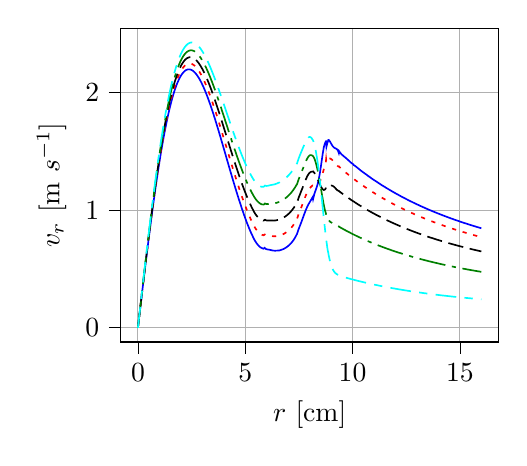
\begin{tikzpicture}

\definecolor{aqua}{RGB}{0,255,255}
\definecolor{darkgray176}{RGB}{176,176,176}
\definecolor{green}{RGB}{0,128,0}

\begin{axis}[
scale = .7,
ylabel = {$v_r$ [m $s^{-1}$]},
xlabel = {$r$ [cm]},
tick align=outside,
tick pos=left,
x grid style={darkgray176},
xmajorgrids,
xmin=-0.799999982118607, xmax=16.7999996244907,
xtick style={color=black},
y grid style={darkgray176},
ymajorgrids,
ymin=-0.122828964870522, ymax=2.54903407004073,
ytick style={color=black}
]
\addplot [semithick, blue]
table {%
	0 -0.00131275799707614
	0.015999999595806 0.0249022428686355
	0.031999999191612 0.0505695969673542
	0.047999998787418 0.0752663217327106
	0.063999998383224 0.0995239790558467
	0.07999999797903 0.123601470635126
	0.095999997574836 0.147693037935212
	0.112000002991408 0.171936219218901
	0.127999996766448 0.196383729926361
	0.14400000218302 0.221184409350581
	0.15999999595806 0.246110258417844
	0.176000001374632 0.271259390001431
	0.191999995149672 0.296304152656856
	0.208000000566244 0.32124570293175
	0.224000005982816 0.345393783631323
	0.239999988116324 0.368988800072476
	0.255999993532896 0.391081456379015
	0.271999998949468 0.417024078673343
	0.28800000436604 0.441605579952123
	0.303999986499548 0.465790590770852
	0.31999999191612 0.489858614455483
	0.335999997332692 0.513732914831301
	0.352000002749264 0.537527736328674
	0.367999984882772 0.561262618167432
	0.383999990299344 0.584953248172042
	0.399999972432852 0.608616157079475
	0.416000001132488 0.632251060719185
	0.431999983265996 0.655835972093962
	0.448000011965632 0.6793782531555
	0.46399999409914 0.702769768576256
	0.479999976232648 0.726053259177499
	0.496000004932284 0.749097596489256
	0.511999987065792 0.771830049301361
	0.5279999691993 0.794334618992957
	0.543999997898936 0.817586755685753
	0.559999980032444 0.840350039409546
	0.57600000873208 0.862909423542718
	0.591999990865588 0.885331328994845
	0.607999972999096 0.907636037580805
	0.624000001698732 0.929768818376631
	0.63999998383224 0.951817383928315
	0.655999965965748 0.973713816541916
	0.671999994665384 0.995499675783184
	0.687999976798892 1.01717780496575
	0.704000005498528 1.03868726354294
	0.719999987632036 1.0601052436886
	0.735999969765544 1.0813254228421
	0.75199999846518 1.10240311751477
	0.767999980598688 1.1233201028741
	0.784000009298325 1.14398430248647
	0.799999944865704 1.16463854457313
	0.81599997356534 1.18510490668364
	0.832000002264977 1.20543097168505
	0.847999937832355 1.22558710957775
	0.863999966531992 1.24553459337692
	0.879999995231628 1.2653649441801
	0.896000023931265 1.28496280697313
	0.911999959498644 1.30442124466175
	0.92799998819828 1.32371750839811
	0.944000016897917 1.3427996932286
	0.959999952465296 1.36176328004981
	0.975999981164932 1.38048370906755
	0.992000009864569 1.39905181567091
	1.00799994543195 1.41744590763256
	1.02399997413158 1.43559528819924
	1.04000000283122 1.45361353004931
	1.0559999383986 1.47136735754598
	1.07199996709824 1.4890048810562
	1.08799999579787 1.50647322200403
	1.10399993136525 1.52367888806079
	1.11999996006489 1.54073005763336
	1.13599998876452 1.55757914430311
	1.15200001746416 1.57418565674489
	1.16799995303154 1.59063570726309
	1.18399998173118 1.60685391698377
	1.20000001043081 1.62285086143549
	1.21599994599819 1.63868935063275
	1.23199997469783 1.65426265362207
	1.24800000339746 1.66963665100672
	1.26399993896484 1.68485095481165
	1.27999996766448 1.69979592603357
	1.29599999636412 1.71456381921386
	1.3119999319315 1.72914277891462
	1.32799996063113 1.74334020793988
	1.34399998933077 1.7575581274772
	1.35999992489815 1.77147806536699
	1.37599995359778 1.78518307440209
	1.39199998229742 1.79863008130904
	1.40800001099706 1.81186092936108
	1.42399994656444 1.82491964691053
	1.43999997526407 1.83772839812007
	1.45600000396371 1.85027964363989
	1.47199993953109 1.86261811565134
	1.48799996823072 1.8747924888859
	1.50399999693036 1.88670254359332
	1.51999993249774 1.89837571800093
	1.53599996119738 1.90976993326419
	1.55199998989701 1.92106115987071
	1.56800001859665 1.93208344226661
	1.58399995416403 1.94290260154515
	1.59999988973141 1.95341665518164
	1.6160000115633 1.96374364677117
	1.63199994713068 1.97373664060584
	1.64799988269806 1.98369690613819
	1.66400000452995 1.99329202356016
	1.67999994009733 2.00276703123802
	1.69599987566471 2.01192971370505
	1.7119999974966 2.02092026788721
	1.72799993306398 2.029649905353
	1.74399986863136 2.03815698562545
	1.75999999046326 2.04645325972515
	1.77599992603064 2.05447863520398
	1.79200004786253 2.06234127952657
	1.80799998342991 2.06988695540096
	1.82399991899729 2.07731592504055
	1.84000004082918 2.0843843015534
	1.85599997639656 2.09137988457508
	1.87199991196394 2.09797330704541
	1.88800003379583 2.10453586660574
	1.90399996936321 2.11071170982271
	1.91999990493059 2.11686518567208
	1.93600002676249 2.12260910187694
	1.95199996232986 2.12829523275817
	1.96799989789724 2.13364200511504
	1.98400001972914 2.13888480565398
	1.99999995529652 2.14373990034488
	2.0159998908639 2.14853035550834
	2.03200001269579 2.1529490997661
	2.04799994826317 2.15727389367729
	2.06399988383055 2.1612794151565
	2.08000000566244 2.16514304822455
	2.09599994122982 2.16874054054342
	2.1119998767972 2.17214712189864
	2.12799999862909 2.17534159237381
	2.14399993419647 2.17831658833647
	2.15999986976385 2.18116533967271
	2.17599999159575 2.18372126076191
	2.19199992716312 2.18617532376654
	2.2079998627305 2.18828340845604
	2.2239999845624 2.19032647982277
	2.23999992012978 2.19200911611699
	2.25600004196167 2.19361931561467
	2.27199997752905 2.19492118939809
	2.28799991309643 2.19609539238977
	2.30400003492832 2.1970288259329
	2.3199999704957 2.19778788662999
	2.33599990606308 2.19835353763059
	2.35200002789497 2.19870015031095
	2.36799996346235 2.1988999767192
	2.38399989902973 2.19883849091154
	2.40000002086163 2.19867566434666
	2.415999956429 2.19821213685046
	2.43199989199638 2.19769114283148
	2.44800001382828 2.19683330152588
	2.46399994939566 2.19592871953605
	2.47999988496304 2.19471721265405
	2.49600000679493 2.19344646569461
	2.51199994236231 2.19192263355931
	2.52799987792969 2.19028863568139
	2.54399999976158 2.18843755546728
	2.55999993532896 2.18645829355167
	2.57599987089634 2.1842645263383
	2.59199999272823 2.18192615714361
	2.60799992829561 2.17937156322891
	2.62399986386299 2.1766946603084
	2.63999998569489 2.17378500208988
	2.65599992126226 2.17077560081055
	2.67199985682964 2.16751752078098
	2.68799997866154 2.16418214765989
	2.70399991422892 2.16060458544425
	2.7199998497963 2.15702223142453
	2.73599997162819 2.15316190690268
	2.75199990719557 2.14926395407249
	2.76800002902746 2.14508385954436
	2.78399996459484 2.14086209488856
	2.79999990016222 2.13638818499874
	2.81600002199411 2.13185229820425
	2.83199995756149 2.12709386917258
	2.84799989312887 2.12225454411077
	2.86400001496077 2.11722143136835
	2.87999995052814 2.11209004714324
	2.89599988609552 2.1067863162661
	2.91200000792742 2.10136712229036
	2.9279999434948 2.09586084997124
	2.94399987906218 2.09013978749983
	2.96000000089407 2.08441100366062
	2.97599993646145 2.07841618465107
	2.99199987202883 2.07239536366375
	3.00799999386072 2.06621448867052
	3.0239999294281 2.05992880444878
	3.03999986499548 2.05356895585905
	3.05599998682737 2.04701204299656
	3.07199992239475 2.04044765640336
	3.08799985796213 2.03364786193491
	3.10399997979403 2.02682339463126
	3.1199999153614 2.01985020562638
	3.1360000371933 2.01277732120675
	3.15199978649616 2.00563396358225
	3.16799990832806 1.99832473204105
	3.18400003015995 1.99100795686381
	3.19999977946281 1.98348145386611
	3.21599990129471 1.97594094058564
	3.2320000231266 1.96826392680219
	3.24799977242947 1.96051295975403
	3.26399989426136 1.95267318084576
	3.28000001609325 1.94465936996507
	3.29599976539612 1.93666331687587
	3.31199988722801 1.92845369167374
	3.32800000905991 1.92030572631022
	3.34399975836277 1.91207642164339
	3.35999988019466 1.90370109620082
	3.37600000202656 1.89534465509091
	3.39199975132942 1.88678245164316
	3.40799987316132 1.87820892314375
	3.42399999499321 1.8695619720708
	3.43999974429607 1.86078184440812
	3.45599986612797 1.85202147525438
	3.47199998795986 1.84307637574343
	3.48799973726273 1.83412100356216
	3.50399985909462 1.82512059655578
	3.51999998092651 1.81606121003657
	3.53600010275841 1.80702285408363
	3.55199985206127 1.79782772071669
	3.56799997389317 1.78861864095459
	3.58400009572506 1.77936857154301
	3.59999984502792 1.77000167716544
	3.61599996685982 1.76065638081856
	3.63200008869171 1.75118596697847
	3.64799983799458 1.7416965644246
	3.66399995982647 1.73219548720045
	3.68000008165836 1.72257222593359
	3.69599983096123 1.71297047156867
	3.71199995279312 1.7032602895387
	3.72800007462502 1.69359112127953
	3.74399982392788 1.6838980672794
	3.75999994575977 1.67414031719078
	3.77600006759167 1.66440329868294
	3.79199981689453 1.6545484549528
	3.80799993872643 1.64471544825679
	3.82400006055832 1.63482727586588
	3.83999980986118 1.6249067409535
	3.85599993169308 1.61498928558429
	3.87200005352497 1.60498992409032
	3.88799980282784 1.59501458148484
	3.90399992465973 1.58497779049872
	3.92000004649162 1.57493358433631
	3.93599979579449 1.56490185328212
	3.95199991762638 1.55485562762623
	3.96800003945827 1.54483358292793
	3.98399978876114 1.53475041259754
	3.99999991059303 1.52467704084422
	4.01600003242493 1.51459160546339
	4.03199978172779 1.50447738621497
	4.04799990355968 1.49438910566527
	4.06400002539158 1.48419336373256
	4.07999977469444 1.47411166497701
	4.09599989652634 1.46395314836527
	4.11200001835823 1.45383434520691
	4.12799976766109 1.44373916274393
	4.14399988949299 1.43366318060952
	4.16000001132488 1.42359149573454
	4.17599976062775 1.41344829756881
	4.19199988245964 1.40332663502103
	4.20800000429153 1.39333746724669
	4.2239997535944 1.3832419430838
	4.23999987542629 1.37301620276652
	4.25599999725819 1.36311688329119
	4.27199974656105 1.35308194273577
	4.28799986839294 1.34295953788453
	4.30399999022484 1.33296504048661
	4.3199997395277 1.32300527257097
	4.3359998613596 1.31299712967731
	4.35199998319149 1.30299959747201
	4.36799973249435 1.29308291199104
	4.38399985432625 1.2832218325541
	4.39999997615814 1.27334271324704
	4.41599972546101 1.26335145727023
	4.4319998472929 1.25362805170424
	4.44799996912479 1.24385987570924
	4.46399971842766 1.23396099910147
	4.47999984025955 1.22425336008271
	4.49599996209145 1.21462371934982
	4.51200008392334 1.20491743883511
	4.5279998332262 1.19524030298749
	4.5439999550581 1.18557029211593
	4.56000007688999 1.17598201346919
	4.57599982619286 1.16651091909036
	4.59199994802475 1.1570639879599
	4.60800006985664 1.14754760960224
	4.62399981915951 1.13805342912121
	4.6399999409914 1.12865634175992
	4.6560000628233 1.11938243344561
	4.67199981212616 1.11010963487227
	4.68799993395805 1.10086466985399
	4.70400005578995 1.09161565702052
	4.71999980509281 1.08243487135826
	4.73599992692471 1.07342205011063
	4.7520000487566 1.06443016348563
	4.76799979805946 1.05538172971902
	4.78399991989136 1.04635417827748
	4.80000004172325 1.03751179280841
	4.81599979102612 1.02872368463411
	4.83199991285801 1.01991460839607
	4.8480000346899 1.01112571526519
	4.86399978399277 1.002471425738
	4.87999990582466 0.99395740534292
	4.89600002765656 0.985430721353084
	4.91199977695942 0.97692064554961
	4.92799989879131 0.968490089930057
	4.94400002062321 0.960250364314111
	4.95999976992607 0.952002612273724
	4.97599989175797 0.94375474317247
	4.99200001358986 0.935542685758499
	5.00799976289272 0.927555010553444
	5.02399988472462 0.919535700292922
	5.04000000655651 0.911499895978571
	5.05599975585938 0.903474915575188
	5.07199987769127 0.895722860852751
	5.08799999952316 0.887775546866229
	5.10399974882603 0.880390694763034
	5.11999987065792 0.873234236844264
	5.13599999248981 0.866084682051625
	5.15199974179268 0.858783413912229
	5.16799986362457 0.851591999389249
	5.18399998545647 0.844428753094472
	5.19999973475933 0.83741623717941
	5.21599985659122 0.830350585742048
	5.23199997842312 0.823318125073864
	5.24799972772598 0.816581988364774
	5.26399984955788 0.809845694815322
	5.27999997138977 0.803397226909101
	5.29599972069263 0.797194462533878
	5.31199984252453 0.790979031047489
	5.32799996435642 0.785544081206087
	5.34399971365929 0.779005890076352
	5.35999983549118 0.772302631176673
	5.37599995732307 0.766129014164137
	5.39199970662594 0.760252561442647
	5.40799982845783 0.754356685016066
	5.42399995028973 0.748758287112101
	5.43999969959259 0.743773296773554
	5.45599982142448 0.738810998234251
	5.47199994325638 0.733871151325981
	5.48799969255924 0.729514710787163
	5.50399981439114 0.725256158936358
	5.51999993622303 0.721017326726935
	5.53600005805492 0.716941571015173
	5.55199980735779 0.71316937901907
	5.56799992918968 0.709420950271471
	5.58400005102158 0.705699344870344
	5.59999980032444 0.702299230495574
	5.61599992215633 0.699064726781326
	5.63200004398823 0.695881101881037
	5.64799979329109 0.692747695840425
	5.66399991512299 0.690084646778998
	5.68000003695488 0.687645944662151
	5.69599978625774 0.685293737535878
	5.71199990808964 0.68300342674915
	5.72800002992153 0.681392295338256
	5.7439997792244 0.679841479682106
	5.75999990105629 0.67832651553623
	5.77600002288818 0.676755962331146
	5.79199977219105 0.675969709351996
	5.80799989402294 0.675106265819893
	5.82400001585484 0.674156081616995
	5.8399997651577 0.671870673959537
	5.85599988698959 0.673237229152148
	5.87200000882149 0.6751115675418
	5.88799975812435 0.677186848566655
	5.90399987995625 0.679464151877624
	5.92000000178814 0.674969243480766
	5.935999751091 0.672959737480164
	5.9519998729229 0.670967981438509
	5.96799999475479 0.669163859583989
	5.98399974405766 0.667919918214215
	5.99999986588955 0.667215353765184
	6.01599998772144 0.666469686013627
	6.03199973702431 0.665762189715876
	6.0479998588562 0.665214964321635
	6.0639999806881 0.664828933478803
	6.07999972999096 0.664425762179614
	6.09599985182285 0.663933936468166
	6.11199997365475 0.663425301125169
	6.12799972295761 0.662906604041032
	6.14399984478951 0.662352729951788
	6.1599999666214 0.661757391977202
	6.17599971592426 0.661075723763349
	6.19199983775616 0.660404486701596
	6.20799995958805 0.659724255925649
	6.22399970889091 0.659035097201317
	6.23999983072281 0.658328087022744
	6.2559999525547 0.657714070084123
	6.2720000743866 0.657144746527217
	6.28800019621849 0.65660057166003
	6.30399957299232 0.656081431975456
	6.31999969482422 0.655700377699375
	6.33599981665611 0.655439779199433
	6.35199993848801 0.655217356330095
	6.3680000603199 0.655032902899694
	6.38400018215179 0.654922541251288
	6.39999955892563 0.654988624302556
	6.41599968075752 0.655070897592278
	6.43199980258942 0.655179974517868
	6.44799992442131 0.655315711969408
	6.4640000462532 0.655522609123976
	6.4800001680851 0.655739312755325
	6.49599954485893 0.65595919055051
	6.51199966669083 0.656194165176717
	6.52799978852272 0.656414721245873
	6.54399991035461 0.656574759285235
	6.56000003218651 0.656746634239565
	6.5760001540184 0.656951325830077
	6.59199953079224 0.657193921765819
	6.60799965262413 0.65808796690047
	6.62399977445602 0.658995901053959
	6.63999989628792 0.659925347588801
	6.65600001811981 0.660844259302529
	6.67200013995171 0.661756488440014
	6.68799951672554 0.662787298021144
	6.70399963855743 0.663839585555099
	6.71999976038933 0.664916764113145
	6.73599988222122 0.666019765380301
	6.75200000405312 0.667206620491551
	6.76800012588501 0.668530378913281
	6.78399950265884 0.669898527057918
	6.79999962449074 0.671304853288083
	6.81599974632263 0.672744102716082
	6.83199986815453 0.674312100426218
	6.84799998998642 0.675979062434778
	6.86400011181831 0.677699665252139
	6.87999948859215 0.679455452101706
	6.89599961042404 0.681244465541368
	6.91199973225594 0.683191508007763
	6.92799985408783 0.685217839634875
	6.94399997591972 0.687305857956028
	6.96000009775162 0.689432459020981
	6.97599947452545 0.691597203361439
	6.99199959635735 0.693959645295233
	7.00799971818924 0.696406349320555
	7.02399984002113 0.698928858045337
	7.03999996185303 0.701501138798225
	7.05600008368492 0.70412276803902
	7.07200020551682 0.706975811087051
	7.08799958229065 0.70993502711562
	7.10399970412254 0.712989832395095
	7.11999982595444 0.716107291992166
	7.13599994778633 0.719286887242073
	7.15200006961823 0.722690585223195
	7.16800019145012 0.726233686056528
	7.18399956822395 0.729900201080364
	7.19999969005585 0.733643621394766
	7.21599981188774 0.737463159626906
	7.23199993371964 0.741454944397222
	7.24800005555153 0.745619099905741
	7.26400017738342 0.749980719217309
	7.27999955415726 0.754450166332775
	7.29599967598915 0.759027009293864
	7.31199979782104 0.763740024328847
	7.32799991965294 0.768646139235048
	7.34400004148483 0.773989079537065
	7.36000016331673 0.779536409987112
	7.37599954009056 0.78528629367134
	7.39199966192245 0.79123772144601
	7.40799978375435 0.79535717084365
	7.42399990558624 0.804937077067411
	7.44000002741814 0.814055993890631
	7.45600014925003 0.822890326918894
	7.47199952602386 0.831437792551942
	7.48799964785576 0.839697317820384
	7.50399976968765 0.846847852544235
	7.51999989151955 0.854257732025427
	7.53600001335144 0.861685522293777
	7.55200013518333 0.869131330961806
	7.56799951195717 0.876594915900841
	7.58399963378906 0.884063698813789
	7.59999975562096 0.891762060865015
	7.61599987745285 0.899529233529732
	7.63199999928474 0.907365583265152
	7.64800012111664 0.915271468716502
	7.66399949789047 0.923277415571503
	7.67999961972237 0.931399530537674
	7.69599974155426 0.939502188660447
	7.71199986338615 0.947609358653127
	7.72799998521805 0.955721060621531
	7.74400010704994 0.963795477405298
	7.75999948382378 0.971737381811927
	7.77599960565567 0.979528301826661
	7.79199972748756 0.98715802538107
	7.80799984931946 0.994711934991302
	7.82399997115135 1.00198097500807
	7.84000009298325 1.0089448521788
	7.85599946975708 1.01579579428633
	7.87199959158897 1.02243871226555
	7.88799971342087 1.02885530290446
	7.90399983525276 1.0347512909535
	7.91999995708466 1.04049716126578
	7.93600007891655 1.04613118015868
	7.95199945569038 1.05165284086405
	7.96799957752228 1.05696182427565
	7.98399969935417 1.06198359926862
	7.99999982118607 1.06692382608975
	8.01599994301796 1.07178237466949
	8.03200006484985 1.07663007195858
	8.04800018668175 1.08165786996111
	8.06399956345558 1.08661137369872
	8.07999968528748 1.09147276508872
	8.09599980711937 1.0962892884902
	8.11199992895126 1.10175053041152
	8.12800005078316 1.10696284919886
	8.14400017261505 1.11192618168785
	8.15999954938889 1.09460870447666
	8.17599967122078 1.10621406704128
	8.19199979305267 1.11793357610788
	8.20799991488457 1.12976904715083
	8.22400003671646 1.14172234224438
	8.24000015854836 1.14971855281328
	8.25599953532219 1.1577103760335
	8.27199965715408 1.16576046695864
	8.28799977898598 1.17386942177104
	8.30399990081787 1.18219088010434
	8.32000002264977 1.19063399884272
	8.33600014448166 1.19919302009181
	8.35199952125549 1.20786955410804
	8.36799964308739 1.21927110133752
	8.38399976491928 1.23093519785595
	8.39999988675117 1.24273147596024
	8.41600000858307 1.2547083340222
	8.43200013041496 1.27049584558816
	8.4479995071888 1.2863917987561
	8.46399962902069 1.30239972565447
	8.47999975085258 1.31892371164428
	8.49599987268448 1.33829404725262
	8.51199999451637 1.3577218734447
	8.52800011634827 1.377156378656
	8.5439994931221 1.39700219342768
	8.55999961495399 1.41762448279158
	8.57599973678589 1.43826000396478
	8.59199985861778 1.45890903072917
	8.60799998044968 1.47820142108225
	8.62400010228157 1.49618752542843
	8.6399994790554 1.51407519818082
	8.6559996008873 1.53186397771002
	8.67199972271919 1.54347212672739
	8.68799984455109 1.55352885745473
	8.70399996638298 1.56342496010847
	8.72000008821487 1.57100364642412
	8.73599946498871 1.56724967297329
	8.7519995868206 1.56338633515917
	8.7679997086525 1.59362094672972
	8.78399983048439 1.5412362664663
	8.79999995231628 1.55299175053279
	8.81600007414818 1.56500579073391
	8.83199945092201 1.57727840333239
	8.84799957275391 1.58127710342417
	8.8639996945858 1.59684204202294
	8.87999981641769 1.59731885889977
	8.89599993824959 1.59699602634863
	8.91200006008148 1.59304188070612
	8.92799943685532 1.58908896435753
	8.94399955868721 1.58513690152967
	8.9599996805191 1.580508184447
	8.975999802351 1.57514673461104
	8.99199992418289 1.56978628845521
	9.00800004601479 1.56442683874948
	9.02400016784668 1.55952179837893
	9.03999954462051 1.55474858866311
	9.05599966645241 1.54997639264872
	9.0719997882843 1.54531439042413
	9.0879999101162 1.54209644755287
	9.10400003194809 1.53888002242316
	9.12000015377998 1.53566510431205
	9.13599953055382 1.53299052354338
	9.15199965238571 1.53127099072574
	9.16799977421761 1.52955306530158
	9.1839998960495 1.52783673603765
	9.20000001788139 1.5263851786075
	9.21600013971329 1.52507730969129
	9.23199951648712 1.52377080742491
	9.24799963831902 1.52246554109841
	9.26399976015091 1.51956484485465
	9.2799998819828 1.5165523590927
	9.2960000038147 1.51354029143865
	9.31200012564659 1.509475859558
	9.32799950242043 1.50161347420023
	9.34399962425232 1.49374947574408
	9.35999974608421 1.48588423875868
	9.37599986791611 1.50148655938327
	9.391999989748 1.4973180721472
	9.4080001115799 1.49314926785144
	9.42399948835373 1.4889803416171
	9.43999961018562 1.48509075966399
	9.45599973201752 1.48196843128512
	9.47199985384941 1.47884593549938
	9.4879999756813 1.47572327281964
	9.5040000975132 1.47262091955456
	9.51999947428703 1.4700467868962
	9.53599959611893 1.4674724731845
	9.55199971795082 1.46489809847676
	9.56799983978271 1.46232366295888
	9.58399996161461 1.45989539660409
	9.6000000834465 1.457502013901
	9.61599946022034 1.45510874915407
	9.63199958205223 1.45271537944466
	9.64799970388412 1.45028999236464
	9.66399982571602 1.44784120807613
	9.67999994754791 1.44539246414448
	9.69600006937981 1.44294376044769
	9.71199944615364 1.44043927161504
	9.72799956798553 1.43782971242848
	9.74399968981743 1.43522019837111
	9.75999981164932 1.43261072930706
	9.77599993348122 1.42998537332612
	9.79200005531311 1.42724066644619
	9.80799943208694 1.42449611262006
	9.82399955391884 1.42175145615555
	9.83999967575073 1.41900682478607
	9.85599979758263 1.41628123401808
	9.87199991941452 1.41355803224852
	9.88800004124641 1.41083481550554
	9.90399941802025 1.40811171064354
	9.91999953985214 1.40559199189285
	9.93599966168404 1.4031780005157
	9.95199978351593 1.4007639378119
	9.96799990534782 1.3983498039935
	9.98400002717972 1.39624748421568
	9.99999940395355 1.39456163306284
	10.0159995257854 1.39287556349839
	10.0319996476173 1.39118935443996
	10.0479997694492 1.38460149183843
	10.0639998912811 1.38273830376948
	10.080000013113 1.38087504183113
	10.0960001349449 1.37901170629883
	10.1119995117188 1.37714838421943
	10.1279996335506 1.37502181638308
	10.1439997553825 1.37278740043621
	10.1599998772144 1.37055294408925
	10.1759999990463 1.36831844749191
	10.1920001208782 1.36604842643331
	10.2079994976521 1.36365304383693
	10.2239996194839 1.36125752238768
	10.2399997413158 1.35886197373368
	10.2559998631477 1.35646639797512
	10.2719999849796 1.35406462094389
	10.2880001068115 1.3516605526539
	10.3039994835854 1.34925656868932
	10.3199996054173 1.34685244525423
	10.3359997272491 1.3444693448637
	10.351999849081 1.34215176588333
	10.3679999709129 1.33983415169043
	10.3840000927448 1.33751650241346
	10.3999994695187 1.33519892610581
	10.4159995913506 1.3329749446488
	10.4319997131824 1.33078141951433
	10.4479998350143 1.3285878506077
	10.4639999568462 1.32639423808762
	10.4800000786781 1.3242283911504
	10.495999455452 1.32213929104556
	10.5119995772839 1.32005004585513
	10.5279996991158 1.3179607530356
	10.5439998209476 1.31587141275865
	10.5599999427795 1.31380336612987
	10.5760000646114 1.31174137549098
	10.5919994413853 1.30967943938516
	10.6079995632172 1.30761736592099
	10.6239996850491 1.30552429543315
	10.639999806881 1.30335522749913
	10.6559999287128 1.30118613967975
	10.6720000505447 1.29901703204602
	10.6879994273186 1.29684800567614
	10.7039995491505 1.29443962018947
	10.7199996709824 1.29197195106706
	10.7359997928143 1.28950430412939
	10.7519999146461 1.28703667929771
	10.768000036478 1.2867657512439
	10.7839994132519 1.28450363922207
	10.7999995350838 1.28224131827961
	10.8159996569157 1.27997889403973
	10.8319997787476 1.2777163667851
	10.8479999005795 1.27556776023434
	10.8640000224113 1.27350269512237
	10.8799993991852 1.27143765697691
	10.8959995210171 1.26937245365762
	10.911999642849 1.26730718151534
	10.9279997646809 1.26533080794589
	10.9439998865128 1.26337124607822
	10.9600000083447 1.26141163738938
	10.9759993851185 1.25945207326042
	10.9919995069504 1.25749653506985
	11.0079996287823 1.25557658641208
	11.0239997506142 1.25365660354426
	11.0399998724461 1.25173658655913
	11.055999994278 1.24981653554868
	11.0720001161098 1.24789629201425
	11.0879994928837 1.24597583597927
	11.1039996147156 1.24405526157864
	11.1199997365475 1.24213465832131
	11.1359998583794 1.24021402628493
	11.1519999802113 1.23828397284591
	11.1680001020432 1.23634844862646
	11.183999478817 1.23441298557267
	11.1999996006489 1.23247740350138
	11.2159997224808 1.23054179261961
	11.2319998443127 1.22860309582262
	11.2479999661446 1.22666401845365
	11.2640000879765 1.22472490884136
	11.2799994647503 1.22278585737022
	11.2959995865822 1.22085218511305
	11.3119997084141 1.21894685333541
	11.327999830246 1.21704148467286
	11.3439999520779 1.21513607922366
	11.3600000739098 1.21323063708545
	11.3759994506836 1.21136670401842
	11.3919995725155 1.20955820825697
	11.4079996943474 1.20774967169185
	11.4239998161793 1.20594109443116
	11.4399999380112 1.20413247658259
	11.4560000598431 1.20245264009892
	11.4719994366169 1.20083006364433
	11.4879995584488 1.199207369362
	11.5039996802807 1.19758463292246
	11.5199998021126 1.19596185443682
	11.5359999239445 1.19327763099669
	11.5520000457764 1.1915554338783
	11.5679994225502 1.18983331416535
	11.5839995443821 1.18811111146868
	11.599999666214 1.18638682108455
	11.6159997880459 1.18464057169358
	11.6319999098778 1.18289431123721
	11.6480000317097 1.18114803972359
	11.6639994084835 1.17940183847752
	11.6799995303154 1.17765614725924
	11.6959996521473 1.17591262944431
	11.7119997739792 1.17416909652686
	11.7279998958111 1.17242554851773
	11.744000017643 1.17068198542749
	11.7599993944168 1.16894605087718
	11.7759995162487 1.16722435574576
	11.7919996380806 1.16550264458124
	11.8079997599125 1.16378091739501
	11.8239998817444 1.16205917419838
	11.8400000035763 1.16035322033395
	11.8559993803501 1.15866480580917
	11.871999502182 1.15697629767997
	11.8879996240139 1.15528777458259
	11.9039997458458 1.15359923652761
	11.9199998676777 1.15193301009697
	11.9359999895096 1.15028137348831
	11.9519993662834 1.14862980074429
	11.9679994881153 1.14697813805351
	11.9839996099472 1.14532646233515
	11.9999997317791 1.14369888703484
	12.015999853611 1.14208002183963
	12.0319999754429 1.14046114531391
	12.0480000972748 1.13884225746588
	12.0639994740486 1.13722343368888
	12.0799995958805 1.1356226639365
	12.0959997177124 1.13402473053027
	12.1119998395443 1.13242678620679
	12.1279999613762 1.13082883097375
	12.1440000832081 1.12923086483885
	12.1599994599819 1.12763433608132
	12.1759995818138 1.12603772771289
	12.1919997036457 1.12444110646625
	12.2079998254776 1.12284447235045
	12.2239999473095 1.1212445833408
	12.2400000691414 1.11962192867439
	12.2559994459152 1.1179993312822
	12.2719995677471 1.11637664005529
	12.287999689579 1.11475393056688
	12.3039998114109 1.11343887883722
	12.3199999332428 1.11187516502177
	12.3360000550747 1.11031147155088
	12.3519994318485 1.10874787129283
	12.3679995536804 1.10718421867564
	12.3839996755123 1.10564043618702
	12.3999997973442 1.10411317001555
	12.4159999191761 1.10258592034634
	12.432000041008 1.10105868722429
	12.4479994177818 1.09953154181007
	12.4639995396137 1.09802707417462
	12.4799996614456 1.09652706688527
	12.4959997832775 1.09502707443873
	12.5119999051094 1.09352709687554
	12.5279992818832 1.09202979502345
	12.5440001487732 1.09055031868087
	12.559999525547 1.08907099487993
	12.576000392437 1.08759154810486
	12.5919997692108 1.08611225394975
	12.6079991459846 1.08463979687482
	12.6240000128746 1.08317682705361
	12.6399993896484 1.08171400922871
	12.6560002565384 1.08025107096149
	12.6719996333122 1.07878828477454
	12.6879990100861 1.07733595979235
	12.703999876976 1.07588791607609
	12.7199992537498 1.07444002437633
	12.7360001206398 1.07299201503915
	12.7519994974136 1.07154415781035
	12.7680003643036 1.07011182614605
	12.7839997410774 1.06867978158732
	12.7999991178513 1.0672477553809
	12.8159999847412 1.06581561420729
	12.831999361515 1.06438897849494
	12.848000228405 1.06297609825898
	12.8639996051788 1.06156336820392
	12.8799989819527 1.06015065680263
	12.8959998488426 1.05873783253611
	12.9119992256165 1.05733938110988
	12.9280000925064 1.05595177110082
	12.9439994692802 1.05456430763818
	12.9600003361702 1.05317673232516
	12.975999712944 1.05178930365247
	12.9919990897179 1.05043050104162
	13.0079999566078 1.04907660854826
	13.0239993333817 1.04772285587365
	13.0400002002716 1.0463689908905
	13.0559995770454 1.04493417258129
	13.0720004439354 1.04358128031253
	13.0879998207092 1.04222973542999
	13.1039991974831 1.04087938894423
	13.120000064373 1.03953009287585
	13.1359994411469 1.03818207670474
	13.1520003080368 1.0368396954983
	13.1679996848106 1.03550651780248
	13.1839990615845 1.03417444800202
	13.1999999284744 1.03284334209034
	13.2159993052483 1.03151342837299
	13.2320001721382 1.03018443996671
	13.247999548912 1.02886487866078
	13.264000415802 1.02755140022594
	13.2799997925758 1.02623905708153
	13.2959991693497 1.02492770910046
	13.3120000362396 1.02361721693453
	13.3279994130135 1.02230780771324
	13.3440002799034 1.02101172396936
	13.3599996566772 1.01971898518838
	13.3759990334511 1.01842719636714
	13.391999900341 1.01713622120854
	13.4079992771149 1.01584628440466
	13.4240001440048 1.01455854663022
	13.4399995207787 1.01328564323772
	13.4560003876686 1.01201352757401
	13.4719997644424 1.01074242160843
	13.4879991412163 1.0094721921883
	13.5040000081062 1.00820240615443
	13.5199993848801 1.00693876027797
	13.53600025177 1.00568589123677
	13.5519996285439 1.00443398107178
	13.5679990053177 1.00318289958527
	13.5839998722076 1.00193251717186
	13.5999992489815 1.00068305379775
	13.6160001158714 0.999443184430967
	13.6319994926453 0.998210267165831
	13.6480003595352 0.99697802730991
	13.6639997363091 0.995746682070747
	13.6799991130829 0.994516104606264
	13.6959999799728 0.9932861686053
	13.7119993567467 0.992069264846568
	13.7280002236366 0.990855109795642
	13.7439996004105 0.989641821225665
	13.7599989771843 0.988429274671175
	13.7759998440742 0.987217346168578
	13.7919992208481 0.986007651984345
	13.808000087738 0.984810006912193
	13.8239994645119 0.983613197434098
	13.8400003314018 0.982416989958537
	13.8559997081757 0.981221596832628
	13.8719990849495 0.980026896374444
	13.8879999518394 0.978837249627627
	13.9039993286133 0.977655910469121
	13.9200001955032 0.976475175522499
	13.9359995722771 0.975295254483711
	13.9519989490509 0.974116027333433
	13.9679998159409 0.972937374499087
	13.9839991927147 0.971784590491854
	14.0000000596046 0.970625167424447
	14.0159994363785 0.969465853435092
	14.0320003032684 0.96830643258102
	14.0479996800423 0.967147120812793
	14.0639990568161 0.965987810158848
	14.0799999237061 0.964830788847895
	14.0959993004799 0.963691478445737
	14.1120001673698 0.962552062963689
	14.1279995441437 0.961412754625177
	14.1440004110336 0.960273341213285
	14.1599997878075 0.959134034951161
	14.1759991645813 0.95799472973195
	14.1920000314713 0.956866915386825
	14.2079994082451 0.955746912140665
	14.224000275135 0.954626805550114
	14.2399996519089 0.953506804242628
	14.2559990286827 0.952386803909289
	14.2719998955727 0.951266700239728
	14.2879992723465 0.95014823167022
	14.3040001392365 0.949046828477538
	14.3199995160103 0.947945528765283
	14.3360003829002 0.946844127394228
	14.3519997596741 0.945742829509086
	14.3679991364479 0.944641532541394
	14.3840000033379 0.943540133924254
	14.3999993801117 0.942449078887996
	14.4160002470016 0.941365872439407
	14.4319996237755 0.940282767725122
	14.4479990005493 0.939199663871402
	14.4639998674393 0.93811646000583
	14.4799992442131 0.937033357881307
	14.4960001111031 0.935950942269388
	14.5119994878769 0.93488561727735
	14.5280003547668 0.93382019387245
	14.5439997315407 0.932754870495935
	14.5599991083145 0.931689547931515
	14.5759999752045 0.93062412696127
	14.5919993519783 0.929558806027507
	14.6080002188683 0.928502561891184
	14.6239995956421 0.927454699536895
	14.6399989724159 0.926406837939603
	14.6559998393059 0.925358879507854
	14.6719992160797 0.924311019431634
	14.6880000829697 0.923263062525267
	14.7039994597435 0.922215323327305
	14.7200003266335 0.921184603117563
	14.7359997034073 0.920153979597861
	14.7519990801811 0.919123356781069
	14.7679999470711 0.918092638682794
	14.7839993238449 0.91706201728026
	14.8000001907349 0.916031300600415
	14.8159995675087 0.915009035386903
	14.8319989442825 0.913995520903211
	14.8479998111725 0.912981912667375
	14.8639991879463 0.911968399469969
	14.8800000548363 0.910954792524939
	14.8959994316101 0.909941280621778
	14.9120002985001 0.908927674975048
	14.9279996752739 0.907930724263578
	14.9439990520477 0.906934285301032
	14.9599999189377 0.905937754106622
	14.9759992957115 0.90494131629191
	14.9920001626015 0.903944786249684
	15.0079995393753 0.902948349590283
	15.0240004062653 0.901954424301477
	15.0399997830391 0.900973147612519
	15.0559991598129 0.899991870643164
	15.0720000267029 0.899010502001016
	15.0879994034767 0.89802922447007
	15.1040002703667 0.897047855265767
	15.1199996471405 0.896071132280093
	15.1359990239143 0.895104712798679
	15.1519998908043 0.894138203036791
	15.1679992675781 0.893171783010901
	15.1840001344681 0.89220527270399
	15.1999995112419 0.891238852132627
	15.2160003781319 0.890274705417867
	15.2319997549057 0.889322928101468
	15.2479991316795 0.888371150522059
	15.2639999985695 0.887419284034715
	15.2799993753433 0.886467505928539
	15.2960002422333 0.885515638913895
	15.3119996190071 0.884564094274097
	15.3279989957809 0.883626732516211
	15.3439998626709 0.882689283202921
	15.3599992394447 0.881751920938078
	15.3760001063347 0.88081447111732
	15.3919994831085 0.879877108344589
	15.4080003499985 0.878939658015428
	15.4239997267723 0.878014645808126
	15.4399991035461 0.877091460901043
	15.4559999704361 0.876168189768597
	15.4719993472099 0.875245004373895
	15.4880002140999 0.874321732753335
	15.5039995908737 0.873398546870117
	15.5199989676476 0.872485471352682
	15.5359998345375 0.871576128998943
	15.5519992113113 0.870666871095969
	15.5680000782013 0.869757528274462
	15.5839994549751 0.868848269903332
	15.6000003218651 0.867938926613196
	15.6159996986389 0.867037604866522
	15.6319990754128 0.866142012782008
	15.6479999423027 0.86524633706157
	15.6639993190765 0.864350744528565
	15.6800001859665 0.863455068359181
	15.6959995627403 0.862559475376859
	15.7119989395142 0.861669715345881
	15.7279998064041 0.860787433424221
	15.7439991831779 0.859905233451894
	15.7600000500679 0.859022951099749
	15.7759994268417 0.858140750696579
	15.7920002937317 0.857258467913154
	15.8079996705055 0.856380073460644
	15.8239990472794 0.855510980996856
	15.8399999141693 0.854641807382291
	15.8559992909431 0.853772714504189
	15.8720001578331 0.852903540474888
	15.8879995346069 0.852034447181702
	15.9039989113808 0.851167213091402
	15.9199997782707 0.850310851548173
	15.9359991550446 0.849454569555363
	15.9520000219345 0.848598207611623
	15.9679993987083 0.847741925217968
	15.9840002655983 0.846885562872972
	15.9999996423721 0.846029280077725
};
\addplot [semithick, red, dash pattern=on 1.5pt off 2.475pt]
table {%
	0 -0.00132386197582797
	0.015999999595806 0.0251940745987047
	0.031999999191612 0.0511601762723603
	0.047999998787418 0.0761480726395701
	0.063999998383224 0.100693473940593
	0.07999999797903 0.125057415161757
	0.095999997574836 0.149435524693549
	0.112000002991408 0.173966570165831
	0.127999996766448 0.198703648373277
	0.14400000218302 0.223796816058722
	0.15999999595806 0.249016329410395
	0.176000001374632 0.274461159662337
	0.191999995149672 0.299801160386149
	0.208000000566244 0.325037492288825
	0.224000005982816 0.349474877816608
	0.239999988116324 0.373355361649614
	0.255999993532896 0.395722711763523
	0.271999998949468 0.421998471223159
	0.28800000436604 0.44686833734068
	0.303999986499548 0.471344913659923
	0.31999999191612 0.4957054082454
	0.335999997332692 0.519873655342354
	0.352000002749264 0.543962931451441
	0.367999984882772 0.567992667104804
	0.383999990299344 0.591978215036478
	0.399999972432852 0.615936106173849
	0.416000001132488 0.639865874386953
	0.431999983265996 0.663745711407846
	0.448000011965632 0.687582997576165
	0.46399999409914 0.71127014355642
	0.479999976232648 0.734849870014547
	0.496000004932284 0.758191851041244
	0.511999987065792 0.781224045518108
	0.5279999691993 0.804029903437129
	0.543999997898936 0.827596305992124
	0.559999980032444 0.850656468377791
	0.57600000873208 0.87351493635859
	0.591999990865588 0.896236961483876
	0.607999972999096 0.918842682443289
	0.624000001698732 0.94127730823656
	0.63999998383224 0.963628082349237
	0.655999965965748 0.985827115546313
	0.671999994665384 1.00791581962636
	0.687999976798892 1.02989703416944
	0.704000005498528 1.05170991159106
	0.719999987632036 1.07343164269917
	0.735999969765544 1.09495626233612
	0.75199999846518 1.11633920884295
	0.767999980598688 1.13756233222054
	0.784000009298325 1.15853465734372
	0.799999944865704 1.17950240367789
	0.81599997356534 1.20027869044313
	0.832000002264977 1.22091497000423
	0.847999937832355 1.24138170399211
	0.863999966531992 1.26164046261411
	0.879999995231628 1.28178257838866
	0.896000023931265 1.30169315484429
	0.911999959498644 1.32146497468653
	0.92799998819828 1.34107537585652
	0.944000016897917 1.36047265072216
	0.959999952465296 1.37975186665041
	0.975999981164932 1.39878887941891
	0.992000009864569 1.41767410095709
	1.00799994543195 1.43638585535467
	1.02399997413158 1.45485349289991
	1.04000000283122 1.47319023481231
	1.0559999383986 1.49126309123821
	1.07199996709824 1.50922596066255
	1.08799999579787 1.52701934360354
	1.10399993136525 1.54454961719655
	1.11999996006489 1.5619257465166
	1.13599998876452 1.57910017825241
	1.15200001746416 1.59603317079772
	1.16799995303154 1.61281048965964
	1.18399998173118 1.62935741408128
	1.20000001043081 1.64568459538438
	1.21599994599819 1.66185430278531
	1.23199997469783 1.67776062888762
	1.24800000339746 1.69346863708624
	1.26399993896484 1.70901773610123
	1.27999996766448 1.72429801228401
	1.29599999636412 1.73940174282337
	1.3119999319315 1.75431739996444
	1.32799996063113 1.7688461965809
	1.34399998933077 1.78340158944453
	1.35999992489815 1.79766241564271
	1.37599995359778 1.81171200401295
	1.39199998229742 1.82550385639132
	1.40800001099706 1.83907979831993
	1.42399994656444 1.8524836942224
	1.43999997526407 1.86563887495928
	1.45600000396371 1.8785378257566
	1.47199993953109 1.89122492590307
	1.48799996823072 1.90374833435616
	1.50399999693036 1.91600875157147
	1.51999993249774 1.92803333265833
	1.53599996119738 1.93978017865527
	1.55199998989701 1.95142359947783
	1.56800001859665 1.96279896530175
	1.58399995416403 1.97397197566279
	1.59999988973141 1.98484086892664
	1.6160000115633 1.99552349862105
	1.63199994713068 2.00587257838263
	1.64799988269806 2.01619144756657
	1.66400000452995 2.02614440327865
	1.67999994009733 2.03597716442453
	1.69599987566471 2.0454980591345
	1.7119999974966 2.0548471088039
	1.72799993306398 2.06393624502903
	1.74399986863136 2.07280365600108
	1.75999999046326 2.08146134618139
	1.77599992603064 2.08984952923839
	1.79200004786253 2.09807585013101
	1.80799998342991 2.10598700717525
	1.82399991899729 2.11378198141514
	1.84000004082918 2.12121829858739
	1.85599997639656 2.12858202035814
	1.87199991196394 2.13554522685782
	1.88800003379583 2.14247760195297
	1.90399996936321 2.14902359713352
	1.91999990493059 2.15554722143613
	1.93600002676249 2.16166084689393
	1.95199996232986 2.16771675077143
	1.96799989789724 2.17343225945845
	1.98400001972914 2.17904672961096
	1.99999995529652 2.18427483999071
	2.0159998908639 2.18943843959134
	2.03200001269579 2.1942316788821
	2.04799994826317 2.19893121875434
	2.06399988383055 2.20331262618871
	2.08000000566244 2.20755257158745
	2.09599994122982 2.21152725043399
	2.1119998767972 2.21531153487196
	2.12799999862909 2.2188842925802
	2.14399993419647 2.2222378676612
	2.15999986976385 2.2254652110129
	2.17599999159575 2.22840001605841
	2.19199992716312 2.23123298091693
	2.2079998627305 2.2337197293848
	2.2239999845624 2.23614121891573
	2.23999992012978 2.23820111238742
	2.25600004196167 2.24019036989933
	2.27199997752905 2.24187261513601
	2.28799991309643 2.24342753976346
	2.30400003492832 2.24474239287786
	2.3199999704957 2.24588321372529
	2.33599990606308 2.24683102976966
	2.35200002789497 2.24756006871532
	2.36799996346235 2.24814254536791
	2.38399989902973 2.24846382827878
	2.40000002086163 2.24868391423088
	2.415999956429 2.24860325755125
	2.43199989199638 2.24846524553207
	2.44800001382828 2.24799021403723
	2.46399994939566 2.2474685222846
	2.47999988496304 2.2466397045391
	2.49600000679493 2.2457515696364
	2.51199994236231 2.24461018024983
	2.52799987792969 2.24335870084837
	2.54399999976158 2.24189016679139
	2.55999993532896 2.24029532869629
	2.57599987089634 2.23848773212277
	2.59199999272823 2.23653503256933
	2.60799992829561 2.23436493296865
	2.62399986386299 2.23207237341179
	2.63999998569489 2.22954599372455
	2.65599992126226 2.22691994764481
	2.67199985682964 2.22404420283676
	2.68799997866154 2.22109140742322
	2.70399991422892 2.21789524755293
	2.7199998497963 2.21469426253946
	2.73599997162819 2.21121443459731
	2.75199990719557 2.20769744875304
	2.76800002902746 2.20389757265239
	2.78399996459484 2.20005644398268
	2.79999990016222 2.19596270940996
	2.81600002199411 2.19180731987864
	2.83199995756149 2.18742922377576
	2.84799989312887 2.18297051112452
	2.86400001496077 2.17831818181864
	2.87999995052814 2.17356791531269
	2.89599988609552 2.16864461465276
	2.91200000792742 2.16360441147003
	2.9279999434948 2.15847695521993
	2.94399987906218 2.15313413378902
	2.96000000089407 2.1477836890858
	2.97599993646145 2.14216636940775
	2.99199987202883 2.13652308163749
	3.00799999386072 2.13071914848302
	3.0239999294281 2.12480997785216
	3.03999986499548 2.1188264267313
	3.05599998682737 2.11264501938608
	3.07199992239475 2.10645623685024
	3.08799985796213 2.10003090435926
	3.10399997979403 2.09358091867161
	3.1199999153614 2.08698142062096
	3.1360000371933 2.08028176233781
	3.15199978649616 2.07351127241362
	3.16799990832806 2.06657386867951
	3.18400003015995 2.05962904663063
	3.19999977946281 2.0524728583929
	3.21599990129471 2.04530274714796
	3.2320000231266 2.03799494529169
	3.24799977242947 2.03061263701936
	3.26399989426136 2.02314380109277
	3.28000001609325 2.01549747316314
	3.29599976539612 2.00786846735068
	3.31199988722801 2.00002614585174
	3.32800000905991 1.99224445999619
	3.34399975836277 1.9843811012192
	3.35999988019466 1.97637147036173
	3.37600000202656 1.96838028299636
	3.39199975132942 1.96018276726921
	3.40799987316132 1.95197346605563
	3.42399999499321 1.94369013334023
	3.43999974429607 1.93527288889119
	3.45599986612797 1.92687494810279
	3.47199998795986 1.91829131461142
	3.48799973726273 1.909696848322
	3.50399985909462 1.90105654738397
	3.51999998092651 1.89235577952496
	3.53600010275841 1.88367552642267
	3.55199985206127 1.87483769055806
	3.56799997389317 1.8659853656675
	3.58400009572506 1.85709160428676
	3.59999984502792 1.84808065182131
	3.61599996685982 1.83909088072409
	3.63200008869171 1.82997630343058
	3.64799983799458 1.82084261107608
	3.66399995982647 1.81169728430765
	3.68000008165836 1.80242537979817
	3.69599983096123 1.7931745625804
	3.71199995279312 1.78381359290746
	3.72800007462502 1.77449255944508
	3.74399982392788 1.76514664746522
	3.75999994575977 1.75573510242373
	3.77600006759167 1.74634391172716
	3.79199981689453 1.73683391929587
	3.80799993872643 1.72734541821411
	3.82400006055832 1.71780112566292
	3.83999980986118 1.70822392183018
	3.85599993169308 1.69864936494106
	3.87200005352497 1.68899210007313
	3.88799980282784 1.67935848047183
	3.90399992465973 1.66966246285675
	3.92000004649162 1.65995842823411
	3.93599979579449 1.65026590866407
	3.95199991762638 1.64055723843677
	3.96800003945827 1.63087234488487
	3.98399978876114 1.62112430975986
	3.99999991059303 1.61138539973607
	4.01600003242493 1.60163295183663
	4.03199978172779 1.59184977138417
	4.04799990355968 1.58209213929366
	4.06400002539158 1.57222711778694
	4.07999977469444 1.56247803110787
	4.09599989652634 1.55265127224517
	4.11200001835823 1.5428614421493
	4.12799976766109 1.53309634339138
	4.14399988949299 1.5233464457499
	4.16000001132488 1.5136008360717
	4.17599976062775 1.50378416835062
	4.19199988245964 1.49398748060023
	4.20800000429153 1.48432147926269
	4.2239997535944 1.47454993646417
	4.23999987542629 1.46464918800264
	4.25599999725819 1.45507007098373
	4.27199974656105 1.44535642619303
	4.28799986839294 1.43555603722778
	4.30399999022484 1.42588159959904
	4.3199997395277 1.41624011344453
	4.3359998613596 1.4065506294307
	4.35199998319149 1.39687179350498
	4.36799973249435 1.3872710104828
	4.38399985432625 1.37772485957484
	4.39999997615814 1.36816072250474
	4.41599972546101 1.3584840358989
	4.4319998472929 1.3490711869429
	4.44799996912479 1.33961348265517
	4.46399971842766 1.33002482223391
	4.47999984025955 1.32062467086967
	4.49599996209145 1.31130499571272
	4.51200008392334 1.30190580359586
	4.5279998332262 1.29253443113399
	4.5439999550581 1.28316918656904
	4.56000007688999 1.27388458920546
	4.57599982619286 1.26471546184231
	4.59199994802475 1.25556969052787
	4.60800006985664 1.2463551287137
	4.62399981915951 1.23716210447768
	4.6399999409914 1.22806478245661
	4.6560000628233 1.21908899511776
	4.67199981212616 1.21011367691581
	4.68799993395805 1.20116522862475
	4.70400005578995 1.19221209614181
	4.71999980509281 1.18332567663181
	4.73599992692471 1.17460439158867
	4.7520000487566 1.16590304876296
	4.76799979805946 1.15714575587711
	4.78399991989136 1.14840892356954
	4.80000004172325 1.13984992958515
	4.81599979102612 1.1313503902751
	4.83199991285801 1.12282646717634
	4.8480000346899 1.11431861124301
	4.86399978399277 1.10594085628814
	4.87999990582466 1.09770081938114
	4.89600002765656 1.08944891337917
	4.91199977695942 1.08121260944866
	4.92799989879131 1.07305448310248
	4.94400002062321 1.06508631819661
	4.95999976992607 1.0571160929496
	4.97599989175797 1.04914751307999
	4.99200001358986 1.04121252367307
	5.00799976289272 1.03349636786226
	5.02399988472462 1.02575390265942
	5.04000000655651 1.01799240678617
	5.05599975585938 1.01023343872775
	5.07199987769127 1.0027350940996
	5.08799999952316 0.995002150797768
	5.10399974882603 0.987793213543011
	5.11999987065792 0.980868830530796
	5.13599999248981 0.973953046660181
	5.15199974179268 0.966921747797871
	5.16799986362457 0.960015765388979
	5.18399998545647 0.953136215470087
	5.19999973475933 0.946403131464942
	5.21599985659122 0.93960695377191
	5.23199997842312 0.932834867979319
	5.24799972772598 0.926306247227919
	5.26399984955788 0.91977747446784
	5.27999997138977 0.91346391964553
	5.29599972069263 0.907343023095813
	5.31199984252453 0.901210848235606
	5.32799996435642 0.895638838019728
	5.34399971365929 0.889561207739551
	5.35999983549118 0.883311193400136
	5.37599995732307 0.877422015557628
	5.39199970662594 0.87174439311268
	5.40799982845783 0.866039195529593
	5.42399995028973 0.860589459744427
	5.43999969959259 0.855686392386002
	5.45599982142448 0.850808807405693
	5.47199994325638 0.84595641917155
	5.48799969255924 0.841684061595403
	5.50399981439114 0.837515294358291
	5.51999993622303 0.83337534072558
	5.53600005805492 0.829411729328563
	5.55199980735779 0.825765613853448
	5.56799992918968 0.822143369830854
	5.58400005102158 0.8185471730263
	5.59999980032444 0.815258947866617
	5.61599992215633 0.812127568533894
	5.63200004398823 0.809038548738007
	5.64799979329109 0.805991349237915
	5.66399991512299 0.803370138788998
	5.68000003695488 0.800965010739934
	5.69599978625774 0.798650571188807
	5.71199990808964 0.796400865413333
	5.72800002992153 0.794780149872808
	5.7439997792244 0.793224139549757
	5.75999990105629 0.791768949546766
	5.77600002288818 0.790357578939133
	5.79199977219105 0.78969227133504
	5.80799989402294 0.788968610240037
	5.82400001585484 0.78817762160501
	5.8399997651577 0.786103165263462
	5.85599988698959 0.786997714179722
	5.87200000882149 0.788581382371771
	5.88799975812435 0.790593133819842
	5.90399987995625 0.793035156113896
	5.92000000178814 0.791846153647541
	5.935999751091 0.789997919495411
	5.9519998729229 0.788065867081851
	5.96799999475479 0.786288283001651
	5.98399974405766 0.785113198856526
	5.99999986588955 0.784557623478107
	6.01599998772144 0.783921971852961
	6.03199973702431 0.783326478552696
	6.0479998588562 0.782945990140089
	6.0639999806881 0.782806207982465
	6.07999972999096 0.782663029120369
	6.09599985182285 0.782439321470359
	6.11199997365475 0.782218827623843
	6.12799972295761 0.782015792405772
	6.14399984478951 0.781783398697867
	6.1599999666214 0.781514758425457
	6.17599971592426 0.781154463361862
	6.19199983775616 0.78077098183111
	6.20799995958805 0.780375324365565
	6.22399970889091 0.779967567771257
	6.23999983072281 0.779535985689126
	6.2559999525547 0.779138235256256
	6.2720000743866 0.778774550802946
	6.28800019621849 0.778433409979073
	6.30399957299232 0.77811470420575
	6.31999969482422 0.777911303357764
	6.33599981665611 0.77781266232663
	6.35199993848801 0.777756613518138
	6.3680000603199 0.777742926886017
	6.38400018215179 0.777808287644679
	6.39999955892563 0.778058778636547
	6.41599968075752 0.778332950040254
	6.43199980258942 0.778640679736128
	6.44799992442131 0.778981788549802
	6.4640000462532 0.779412101150117
	6.4800001680851 0.779855104395329
	6.49599954485893 0.780298161751171
	6.51199966669083 0.780752747095244
	6.52799978852272 0.781185435095202
	6.54399991035461 0.781531333780566
	6.56000003218651 0.781869303698849
	6.5760001540184 0.782224440050518
	6.59199953079224 0.782601740188797
	6.60799965262413 0.783676649209466
	6.62399977445602 0.784782990106873
	6.63999989628792 0.785881623663092
	6.65600001811981 0.78698039263658
	6.67200013995171 0.788082545389961
	6.68799951672554 0.789291699619098
	6.70399963855743 0.79051602340081
	6.71999976038933 0.791758329142075
	6.73599988222122 0.793024114119326
	6.75200000405312 0.79436650921021
	6.76800012588501 0.795834686909989
	6.78399950265884 0.797343995882593
	6.79999962449074 0.798891108141155
	6.81599974632263 0.800471662208832
	6.83199986815453 0.802178516364463
	6.84799998998642 0.803982833344746
	6.86400011181831 0.805839388469661
	6.87999948859215 0.807731575780685
	6.89599961042404 0.809657623691671
	6.91199973225594 0.811736260729594
	6.92799985408783 0.813890440179406
	6.94399997591972 0.816097018900988
	6.96000009775162 0.818339781608553
	6.97599947452545 0.8206183045905
	6.99199959635735 0.823080147945067
	7.00799971818924 0.825617302218377
	7.02399984002113 0.828215206536509
	7.03999996185303 0.830857959770332
	7.05600008368492 0.83354518027338
	7.07200020551682 0.836447079990065
	7.08799958229065 0.839444124034933
	7.10399970412254 0.842521428367251
	7.11999982595444 0.845655245447078
	7.13599994778633 0.848845107450777
	7.15200006961823 0.852246800138169
	7.16800019145012 0.855776541231677
	7.18399956822395 0.859415190661959
	7.19999969005585 0.863121733100698
	7.21599981188774 0.866895454884119
	7.23199993371964 0.870828182406605
	7.24800005555153 0.874916513025991
	7.26400017738342 0.879186875819468
	7.27999955415726 0.883548656483607
	7.29599967598915 0.888001541911479
	7.31199979782104 0.892566954772407
	7.32799991965294 0.897283169828001
	7.34400004148483 0.902436121869839
	7.36000016331673 0.907769921316288
	7.37599954009056 0.913282923028059
	7.39199966192245 0.918974273721834
	7.40799978375435 0.921984807032588
	7.42399990558624 0.931783878960864
	7.44000002741814 0.940707442460984
	7.45600014925003 0.949472987814706
	7.47199952602386 0.958079067279495
	7.48799964785576 0.966525444582133
	7.50399976968765 0.973791838945393
	7.51999989151955 0.981275416727217
	7.53600001335144 0.988770933609977
	7.55200013518333 0.99627846132669
	7.56799951195717 1.00379772000276
	7.58399963378906 1.01123691958663
	7.59999975562096 1.01877776570995
	7.61599987745285 1.02637479682758
	7.63199999928474 1.03402831215788
	7.64800012111664 1.04173860454051
	7.66399949789047 1.0495328774968
	7.67999961972237 1.05742223926633
	7.69599974155426 1.06528757712333
	7.71199986338615 1.07315671112132
	7.72799998521805 1.08102965817668
	7.74400010704994 1.08888559460086
	7.75999948382378 1.09665453786563
	7.77599960565567 1.10426615857499
	7.79199972748756 1.11171272359649
	7.80799984931946 1.11907858614969
	7.82399997115135 1.1261715432648
	7.84000009298325 1.13295439325962
	7.85599946975708 1.13959768584867
	7.87199959158897 1.14600451363436
	7.88799971342087 1.15215725027566
	7.90399983525276 1.15765380365719
	7.91999995708466 1.16293878481675
	7.93600007891655 1.16805957525574
	7.95199945569038 1.17301557773198
	7.96799957752228 1.17754045488181
	7.98399969935417 1.18151889774882
	7.99999982118607 1.18534674835458
	8.01599994301796 1.18902376650401
	8.03200006484985 1.1925027357846
	8.04800018668175 1.1956641691508
	8.06399956345558 1.19868079331409
	8.07999968528748 1.20148303140584
	8.09599980711937 1.20407599309912
	8.11199992895126 1.20664282302241
	8.12800005078316 1.2089523995377
	8.14400017261505 1.21100465736681
	8.15999954938889 1.21067782765788
	8.17599967122078 1.21184313944433
	8.19199979305267 1.21300936103826
	8.20799991488457 1.21417650691136
	8.22400003671646 1.21534459190393
	8.24000015854836 1.21517082707605
	8.25599953532219 1.21497728442249
	8.27199965715408 1.21478935047463
	8.28799977898598 1.21460712820579
	8.30399990081787 1.21486139631879
	8.32000002264977 1.21518551164798
	8.33600014448166 1.21555535061643
	8.35199952125549 1.21597168848568
	8.36799964308739 1.21798307145303
	8.38399976491928 1.22014247294278
	8.39999988675117 1.22237269400058
	8.41600000858307 1.22470275245234
	8.43200013041496 1.22933248581185
	8.4479995071888 1.23404137680578
	8.46399962902069 1.23883135557889
	8.47999975085258 1.24400190690809
	8.49599987268448 1.25129687694215
	8.51199999451637 1.25866617190023
	8.52800011634827 1.26614840775983
	8.5439994931221 1.27429299225737
	8.55999961495399 1.28382126877081
	8.57599973678589 1.29339949289197
	8.59199985861778 1.30302869809636
	8.60799998044968 1.31319028581054
	8.62400010228157 1.32381061590226
	8.6399994790554 1.33444765778078
	8.6559996008873 1.34510277724556
	8.67199972271919 1.35547210796662
	8.68799984455109 1.36579373077789
	8.70399996638298 1.37613847114525
	8.72000008821487 1.38620587280465
	8.73599946498871 1.39477634589916
	8.7519995868206 1.40345090824969
	8.7679997086525 1.4335087531715
	8.78399983048439 1.40835860435461
	8.79999995231628 1.41270143652474
	8.81600007414818 1.41711469503689
	8.83199945092201 1.42159833119682
	8.84799957275391 1.42480006416581
	8.8639996945858 1.43572695207092
	8.87999981641769 1.43798225452705
	8.89599993824959 1.43984428545524
	8.91200006008148 1.43990516337658
	8.92799943685532 1.43996572890151
	8.94399955868721 1.44002598992624
	8.9599996805191 1.43928046911909
	8.975999802351 1.4376619417217
	8.99199992418289 1.43604231750928
	9.00800004601479 1.43442160438275
	9.02400016784668 1.43189883437628
	9.03999954462051 1.42911726770888
	9.05599966645241 1.42633589993197
	9.0719997882843 1.42350864251993
	9.0879999101162 1.42007094580159
	9.10400003194809 1.41663564429617
	9.12000015377998 1.41320272108134
	9.13599953055382 1.40970805878271
	9.15199965238571 1.40610271141048
	9.16799977421761 1.40250098879369
	9.1839998960495 1.39890286560079
	9.20000001788139 1.39548413524088
	9.21600013971329 1.39216333426132
	9.23199951648712 1.38884536832117
	9.24799963831902 1.38552990986695
	9.26399976015091 1.38285283818052
	9.2799998819828 1.38021892367512
	9.2960000038147 1.37758334745821
	9.31200012564659 1.37517340497514
	9.32799950242043 1.37357630256966
	9.34399962425232 1.37196853265779
	9.35999974608421 1.37035024126164
	9.37599986791611 1.37094263398547
	9.391999989748 1.36783702895928
	9.4080001115799 1.36473139020701
	9.42399948835373 1.36162586245131
	9.43999961018562 1.35861200681869
	9.45599973201752 1.35585000096204
	9.47199985384941 1.35308794833562
	9.4879999756813 1.35032584908272
	9.5040000975132 1.34757191249402
	9.51999947428703 1.3450298231206
	9.53599959611893 1.34248757776302
	9.55199971795082 1.33994529491499
	9.56799983978271 1.33740297469079
	9.58399996161461 1.33495981306656
	9.6000000834465 1.33254029667636
	9.61599946022034 1.33012087676277
	9.63199958205223 1.32770132804009
	9.64799970388412 1.32531196788537
	9.66399982571602 1.32294470985348
	9.67999994754791 1.32057745946658
	9.69600006937981 1.31821021670155
	9.71199944615364 1.31584596328672
	9.72799956798553 1.31348700875554
	9.74399968981743 1.31112807895695
	9.75999981164932 1.30876917381651
	9.77599993348122 1.3064091955373
	9.79200005531311 1.30404101691741
	9.80799943208694 1.3016729746807
	9.82399955391884 1.29930484819915
	9.83999967575073 1.29693674767024
	9.85599979758263 1.29456821471963
	9.87199991941452 1.29219962828636
	9.88800004124641 1.28983104497305
	9.90399941802025 1.28746257506505
	9.91999953985214 1.28511678786739
	9.93599966168404 1.28278280333634
	9.95199978351593 1.28044876641593
	9.96799990534782 1.27811467726188
	9.98400002717972 1.27582167562702
	9.99999940395355 1.27358359741454
	10.0159995257854 1.27134526646771
	10.0319996476173 1.26910678744555
	10.0479997694492 1.2671022948297
	10.0639998912811 1.26485494740898
	10.080000013113 1.26260742234547
	10.0960001349449 1.26035972030157
	10.1119995117188 1.25811194661471
	10.1279996335506 1.25590793899637
	10.1439997553825 1.25372189034198
	10.1599998772144 1.25153576690286
	10.1759999990463 1.24934956895615
	10.1920001208782 1.24717372514515
	10.2079994976521 1.24503480208394
	10.2239996194839 1.24289575438831
	10.2399997413158 1.24075668175524
	10.2559998631477 1.23861758427659
	10.2719999849796 1.23650475369804
	10.2880001068115 1.23440154818012
	10.3039994835854 1.2322984281548
	10.3199996054173 1.23019519779175
	10.3359997272491 1.22809877710742
	10.351999849081 1.22602358238375
	10.3679999709129 1.22394836517259
	10.3840000927448 1.22187312555598
	10.3999994695187 1.21979796025226
	10.4159995913506 1.21774063211708
	10.4319997131824 1.21568910750219
	10.4479998350143 1.2136375419211
	10.4639999568462 1.21158593552234
	10.4800000786781 1.20954046953744
	10.495999455452 1.20751209545605
	10.5119995772839 1.20548357217217
	10.5279996991158 1.20345499433931
	10.5439998209476 1.20142636215407
	10.5599999427795 1.19941823249213
	10.5760000646114 1.19741592565755
	10.5919994413853 1.19541366127425
	10.6079995632172 1.19341125304177
	10.6239996850491 1.1914184916543
	10.639999806881 1.18944949966271
	10.6559999287128 1.18748049034167
	10.6720000505447 1.18551146375303
	10.6879994273186 1.18354251164883
	10.7039995491505 1.18160913452606
	10.7199996709824 1.1796846527194
	10.7359997928143 1.17776022825092
	10.7519999146461 1.17583586091709
	10.768000036478 1.17409659000188
	10.7839994132519 1.17216096327573
	10.7999995350838 1.17022521485136
	10.8159996569157 1.16828943495266
	10.8319997787476 1.16635362366575
	10.8479999005795 1.16444764137364
	10.8640000224113 1.16256351179167
	10.8799993991852 1.16067942136453
	10.8959995210171 1.15879519474838
	10.911999642849 1.15691091981218
	10.9279997646809 1.15506003812536
	10.9439998865128 1.15321544149219
	10.9600000083447 1.1513707921123
	10.9759993851185 1.14952617603007
	10.9919995069504 1.14768465351471
	11.0079996287823 1.14587073625163
	11.0239997506142 1.14405677038013
	11.0399998724461 1.14224275603191
	11.055999994278 1.14042869333778
	11.0720001161098 1.13862382304251
	11.0879994928837 1.13683480668743
	11.1039996147156 1.13504566688332
	11.1199997365475 1.13325648704816
	11.1359998583794 1.13146726728966
	11.1519999802113 1.12969209646908
	11.1680001020432 1.12792505506388
	11.183999478817 1.12615806437591
	11.1999996006489 1.1243909599198
	11.2159997224808 1.12262382406405
	11.2319998443127 1.12087680861769
	11.2479999661446 1.11913206276288
	11.2640000879765 1.1173872900784
	11.2799994647503 1.11564257188443
	11.2959995865822 1.11390190632287
	11.3119997084141 1.11218267111392
	11.327999830246 1.11046340613749
	11.3439999520779 1.10874411147291
	11.3600000739098 1.10702478719895
	11.3759994506836 1.10531907431415
	11.3919995725155 1.10363141747131
	11.4079996943474 1.10194371675287
	11.4239998161793 1.10025597227505
	11.4399999380112 1.09856818415365
	11.4560000598431 1.09690858204077
	11.4719994366169 1.09526152867764
	11.4879995584488 1.09361432590514
	11.5039996802807 1.09196705061324
	11.5199998021126 1.09031970299303
	11.5359999239445 1.08857431201107
	11.5520000457764 1.08694233615707
	11.5679994225502 1.08531042125896
	11.5839995443821 1.08367841533758
	11.599999666214 1.08204786746592
	11.6159997880459 1.08043281490001
	11.6319999098778 1.0788177483083
	11.6480000317097 1.07720266770101
	11.6639994084835 1.07558764829627
	11.6799995303154 1.07397691893024
	11.6959996521473 1.07238207425183
	11.7119997739792 1.0707872158807
	11.7279998958111 1.06919234382665
	11.744000017643 1.06759745809927
	11.7599993944168 1.06601041741718
	11.7759995162487 1.06443804593553
	11.7919996380806 1.06286566065469
	11.8079997599125 1.06129326158443
	11.8239998817444 1.05972084873449
	11.8400000035763 1.05815971283625
	11.8559993803501 1.05661111919374
	11.871999502182 1.05506243933755
	11.8879996240139 1.05351374539212
	11.9039997458458 1.05196503736743
	11.9199998676777 1.05043081310752
	11.9359999895096 1.04890605721866
	11.9519993662834 1.04738135798564
	11.9679994881153 1.04585657341444
	11.9839996099472 1.04433177451691
	11.9999997317791 1.04282396930866
	12.015999853611 1.04132230147123
	12.0319999754429 1.03982061933465
	12.0480000972748 1.03831892290918
	12.0639994740486 1.03681728213337
	12.0799995958805 1.03533397938257
	12.0959997177124 1.03385355434895
	12.1119998395443 1.03237311559776
	12.1279999613762 1.03089266313867
	12.1440000832081 1.02941219698133
	12.1599994599819 1.02795012915357
	12.1759995818138 1.02648808257078
	12.1919997036457 1.02502602362367
	12.2079998254776 1.02356395232095
	12.2239999473095 1.02210368409288
	12.2400000691414 1.02065614386265
	12.2559994459152 1.01920866102687
	12.2719995677471 1.01776110078021
	12.287999689579 1.01631353053555
	12.3039998114109 1.01491242134024
	12.3199999332428 1.01348834017884
	12.3360000550747 1.01206427450581
	12.3519994318485 1.01064029067474
	12.3679995536804 1.00921625610374
	12.3839996755123 1.00780419854792
	12.3999997973442 1.00640209920209
	12.4159999191761 1.00500001592083
	12.432000041008 1.00359794874783
	12.4479994177818 1.00219596301416
	12.4639995396137 1.00081068305993
	12.4799996614456 0.999428695951137
	12.4959997832775 0.998046725256307
	12.5119999051094 0.996664771020278
	12.5279992818832 0.995285243597927
	12.5440001487732 0.993921857116385
	12.559999525547 0.992558614162249
	12.576000392437 0.991195260847239
	12.5919997692108 0.989832051147496
	12.6079991459846 0.988476167714314
	12.6240000128746 0.987130470022703
	12.6399993896484 0.985784914317941
	12.6560002565384 0.984439250006579
	12.6719996333122 0.983093727770881
	12.6879990100861 0.981760220115958
	12.703999876976 0.980431658485851
	12.7199992537498 0.979103237343864
	12.7360001206398 0.977774709288989
	12.7519994974136 0.976446321811967
	12.7680003643036 0.9751346219088
	12.7839997410774 0.973823206427137
	12.7999991178513 0.972511807873206
	12.8159999847412 0.971200304158118
	12.831999361515 0.969893748595966
	12.848000228405 0.968599547262514
	12.8639996051788 0.967305483651853
	12.8799989819527 0.966011437285283
	12.8959998488426 0.964717287691608
	12.9119992256165 0.963433465495316
	12.9280000925064 0.962157389253477
	12.9439994692802 0.960881449595715
	12.9600003361702 0.95960540890016
	12.975999712944 0.95832950488488
	12.9919990897179 0.957069993045429
	13.0079999566078 0.955813257184099
	13.0239993333817 0.954556656977123
	13.0400002002716 0.95329995840769
	13.0559995770454 0.952027247702361
	13.0720004439354 0.950784620705471
	13.0879998207092 0.949543209749987
	13.1039991974831 0.948302878394976
	13.120000064373 0.947063491109419
	13.1359994411469 0.945825259066446
	13.1520003080368 0.944592530876003
	13.1679996848106 0.943368887311746
	13.1839990615845 0.942146317577007
	13.1999999284744 0.940924688476794
	13.2159993052483 0.939704208529372
	13.2320001721382 0.938484631824971
	13.247999548912 0.93727400922126
	13.264000415802 0.936069229396401
	13.2799997925758 0.934865564416174
	13.2959991693497 0.933662884457751
	13.3120000362396 0.932461060469265
	13.3279994130135 0.931260299513064
	13.3440002799034 0.930071724619517
	13.3599996566772 0.928886272454803
	13.3759990334511 0.927701764521979
	13.391999900341 0.92651807461204
	13.4079992771149 0.925335407529733
	13.4240001440048 0.924154787954237
	13.4399995207787 0.922987467287924
	13.4560003876686 0.92182094146821
	13.4719997644424 0.920655412842701
	13.4879991412163 0.919490758136014
	13.5040000081062 0.918326526819385
	13.5199993848801 0.917167812155518
	13.53600025177 0.916018732487527
	13.5519996285439 0.914870600618659
	13.5679990053177 0.913723296039445
	13.5839998722076 0.912576698831798
	13.5999992489815 0.911431009653113
	13.6160001158714 0.910293992994768
	13.6319994926453 0.909163291134409
	13.6480003595352 0.908033278505066
	13.6639997363091 0.906904153238264
	13.6799991130829 0.905775797976942
	13.6959999799728 0.904648095896498
	13.7119993567467 0.903532419940337
	13.7280002236366 0.902419327273573
	13.7439996004105 0.901307088736775
	13.7599989771843 0.900195589320595
	13.7759998440742 0.899084714515592
	13.7919992208481 0.897975993165469
	13.808000087738 0.896878775729215
	13.8239994645119 0.895782367757746
	13.8400003314018 0.894686554608497
	13.8559997081757 0.893591530171868
	13.8719990849495 0.892497182353627
	13.8879999518394 0.891407901536076
	13.9039993286133 0.890326911176892
	13.9200001955032 0.88924648273827
	13.9359995722771 0.888166807972593
	13.9519989490509 0.887087776929168
	13.9679998159409 0.88600928007175
	13.9839991927147 0.884948471281485
	14.0000000596046 0.883886758431265
	14.0159994363785 0.882825145538655
	14.0320003032684 0.881763434859672
	14.0479996800423 0.880701824145864
	14.0639990568161 0.87964021452517
	14.0799999237061 0.878580719616868
	14.0959993004799 0.877537577023562
	14.1120001673698 0.876494338295444
	14.1279995441437 0.87545119774262
	14.1440004110336 0.874407961061411
	14.1599997878075 0.873364822561644
	14.1759991645813 0.872321685093064
	14.1920000314713 0.871289205614828
	14.2079994082451 0.870263968983742
	14.224000275135 0.86923863782678
	14.2399996519089 0.868213403119055
	14.2559990286827 0.867188169377749
	14.2719998955727 0.866162841118733
	14.2879992723465 0.865139032602929
	14.3040001392365 0.864131102795917
	14.3199995160103 0.863123267756814
	14.3360003829002 0.862115339756271
	14.3519997596741 0.861107506529068
	14.3679991364479 0.860099674211691
	14.3840000033379 0.859091748942094
	14.3999993801117 0.858093462925149
	14.4160002470016 0.857102494123535
	14.4319996237755 0.856111618456695
	14.4479990005493 0.855120743640721
	14.4639998674393 0.854129777392946
	14.4799992442131 0.853138904286673
	14.4960001111031 0.852148673085283
	14.5119994878769 0.851174375041773
	14.5280003547668 0.850199987051145
	14.5439997315407 0.849225690598939
	14.5599991083145 0.848251394946615
	14.5759999752045 0.847277009354143
	14.5919993519783 0.846302715308018
	14.6080002188683 0.845336875110742
	14.6239995956421 0.844378838272637
	14.6399989724159 0.843420802178567
	14.6559998393059 0.842462677603042
	14.6719992160797 0.841504643003997
	14.6880000829697 0.840546519927767
	14.7039994597435 0.839588597638742
	14.7200003266335 0.838646477665809
	14.7359997034073 0.837704446121669
	14.7519990801811 0.836762415270343
	14.7679999470711 0.835820297378397
	14.7839993238449 0.834878267920904
	14.8000001907349 0.833936151426926
	14.8159995675087 0.833001843963402
	14.8319989442825 0.832075623045558
	14.8479998111725 0.831149316504213
	14.8639991879463 0.830223096869645
	14.8800000548363 0.829296791616058
	14.8959994316101 0.828370573272713
	14.9120002985001 0.827444269314406
	14.9279996752739 0.826533257963377
	14.9439990520477 0.82562271657445
	14.9599999189377 0.824712090969149
	14.9759992957115 0.823801550758677
	14.9920001626015 0.82289092633623
	15.0079995393753 0.821980387311865
	15.0240004062653 0.821073863899194
	15.0399997830391 0.820177648840831
	15.0559991598129 0.819281433502204
	15.0720000267029 0.81838513441321
	15.0879994034767 0.817488918513263
	15.1040002703667 0.816592618862384
	15.1199996471405 0.815700644617297
	15.1359990239143 0.81481826611061
	15.1519998908043 0.813935805152876
	15.1679992675781 0.813053426106107
	15.1840001344681 0.812170964607747
	15.1999995112419 0.811288585019906
	15.2160003781319 0.810408322551208
	15.2319997549057 0.809539566873507
	15.2479991316795 0.808670810936104
	15.2639999985695 0.807801973826371
	15.2799993753433 0.806933217368825
	15.2960002422333 0.806064379738424
	15.3119996190071 0.805195840316776
	15.3279989957809 0.804340487473636
	15.3439998626709 0.803485054716805
	15.3599992394447 0.802629701374187
	15.3760001063347 0.801774268117373
	15.3919994831085 0.800918914274359
	15.4080003499985 0.800063480516642
	15.4239997267723 0.799219605534411
	15.4399991035461 0.798377428872037
	15.4559999704361 0.797535173532854
	15.4719993472099 0.796692996390425
	15.4880002140999 0.7958507405707
	15.5039995908737 0.795008562947331
	15.5199989676476 0.794175781918982
	15.5359998345375 0.793346471967599
	15.5519992113113 0.792517239017493
	15.5680000782013 0.79168792860576
	15.5839994549751 0.790858695194923
	15.6000003218651 0.790029384321991
	15.6159996986389 0.789207529702333
	15.6319990754128 0.788391002036341
	15.6479999423027 0.787574398101969
	15.6639993190765 0.786757869995108
	15.6800001859665 0.785941265619418
	15.6959995627403 0.785124737070872
	15.7119989395142 0.784313635390706
	15.7279998064041 0.783509492764106
	15.7439991831779 0.782705424814327
	15.7600000500679 0.781901281766014
	15.7759994268417 0.781097213394171
	15.7920002937317 0.780293069923365
	15.8079996705055 0.779492546489824
	15.8239990472794 0.778700687155673
	15.8399999141693 0.777908753869655
	15.8559992909431 0.777116894132661
	15.8720001578331 0.776324960443389
	15.8879995346069 0.775533100302804
	15.9039989113808 0.774742974558495
	15.9199997782707 0.773962993298244
	15.9359991550446 0.77318308448348
	15.9520000219345 0.772403102839028
	15.9679993987083 0.771623193639741
	15.9840002655983 0.770843211610373
	15.9999996423721 0.770063302025848
};
\addplot [semithick, black, dash pattern=on 5.55pt off 2.4pt]
table {%
	0 -0.00134054606955631
	0.015999999595806 0.0255035778064527
	0.031999999191612 0.0517888434096023
	0.047999998787418 0.0770831956544833
	0.063999998383224 0.101929393532168
	0.07999999797903 0.126591944227281
	0.095999997574836 0.151269099421213
	0.112000002991408 0.176101534317687
	0.127999996766448 0.201143086599666
	0.14400000218302 0.226546047053507
	0.15999999595806 0.252077495773978
	0.176000001374632 0.277838156252326
	0.191999995149672 0.3034934209912
	0.208000000566244 0.329044457067426
	0.224000005982816 0.353787456743511
	0.239999988116324 0.377967007252006
	0.255999993532896 0.400614966888519
	0.271999998949468 0.427220429499262
	0.28800000436604 0.452410440130446
	0.303999986499548 0.477200961459424
	0.31999999191612 0.50187412782574
	0.335999997332692 0.526352792397504
	0.352000002749264 0.550752409440921
	0.367999984882772 0.575092408420499
	0.383999990299344 0.599389680506487
	0.399999972432852 0.623660109007119
	0.416000001132488 0.647904237153079
	0.431999983265996 0.672099722293736
	0.448000011965632 0.696253632935133
	0.46399999409914 0.720258112272695
	0.479999976232648 0.744154923730326
	0.496000004932284 0.767812762635028
	0.511999987065792 0.791157805508407
	0.5279999691993 0.814274383132501
	0.543999997898936 0.838162330135617
	0.559999980032444 0.861542293829997
	0.57600000873208 0.88472061250513
	0.591999990865588 0.907762962131506
	0.607999972999096 0.930689429771762
	0.624000001698732 0.953445874197793
	0.63999998383224 0.976119049010491
	0.655999965965748 0.99864174443881
	0.671999994665384 1.02105504905875
	0.687999976798892 1.04336177026565
	0.704000005498528 1.06550149346128
	0.719999987632036 1.08755066608423
	0.735999969765544 1.10940388191209
	0.75199999846518 1.13111592656832
	0.767999980598688 1.15266869201496
	0.784000009298325 1.1739708093819
	0.799999944865704 1.19527193692894
	0.81599997356534 1.21637768951806
	0.832000002264977 1.23734495083597
	0.847999937832355 1.25814438390535
	0.863999966531992 1.27873741532915
	0.879999995231628 1.29921454084626
	0.896000023931265 1.31946139884996
	0.911999959498644 1.33957012689824
	0.92799998819828 1.3595181732499
	0.944000016897917 1.37925412090568
	0.959999952465296 1.39887259169566
	0.975999981164932 1.41825029181046
	0.992000009864569 1.43747727402546
	1.00799994543195 1.45653207339152
	1.02399997413158 1.47534502242156
	1.04000000283122 1.4940283408591
	1.0559999383986 1.51245064454639
	1.07199996709824 1.5307595552101
	1.08799999579787 1.54889823598371
	1.10399993136525 1.56677507952654
	1.11999996006489 1.58449864891125
	1.13599998876452 1.60202186693679
	1.15200001746416 1.61930537104959
	1.16799995303154 1.63643434375224
	1.18399998173118 1.65333456751615
	1.20000001043081 1.67001646353614
	1.21599994599819 1.68654185817135
	1.23199997469783 1.70280520552047
	1.24800000339746 1.7188710065843
	1.26399993896484 1.73477840200506
	1.27999996766448 1.75041676539805
	1.29599999636412 1.76587838912644
	1.3119999319315 1.78115180455505
	1.32799996063113 1.79604569743476
	1.34399998933077 1.81096582962107
	1.35999992489815 1.82559094939674
	1.37599995359778 1.84000147503079
	1.39199998229742 1.85415495107726
	1.40800001099706 1.86809400872439
	1.42399994656444 1.88186281560607
	1.43999997526407 1.89538428673889
	1.45600000396371 1.90865088120172
	1.47199993953109 1.92170647171886
	1.48799996823072 1.93459869928348
	1.50399999693036 1.94722889577852
	1.51999993249774 1.95962419518848
	1.53599996119738 1.97174318209629
	1.55199998989701 1.98375886835653
	1.56800001859665 1.99550862893908
	1.58399995416403 2.00705735053493
	1.59999988973141 2.01830569005018
	1.6160000115633 2.02936921531911
	1.63199994713068 2.04009858451234
	1.64799988269806 2.05079513220321
	1.66400000452995 2.06112830920514
	1.67999994009733 2.07134199367647
	1.69599987566471 2.08124520569866
	1.7119999974966 2.09097730267982
	1.72799993306398 2.10045020964119
	1.74399986863136 2.10970200417136
	1.75999999046326 2.11874447974784
	1.77599992603064 2.12751794876558
	1.79200004786253 2.13612983130652
	1.80799998342991 2.14442707171639
	1.82399991899729 2.15260836004296
	1.84000004082918 2.16043178450157
	1.85599997639656 2.16818277823367
	1.87199991196394 2.17553464839863
	1.88800003379583 2.1828556840616
	1.90399996936321 2.18979240018386
	1.91999990493059 2.19670670746207
	1.93600002676249 2.20321430444426
	1.95199996232986 2.20966430988281
	1.96799989789724 2.21577930955485
	1.98400001972914 2.22179171966274
	1.99999995529652 2.22741618884285
	2.0159998908639 2.23297598275856
	2.03200001269579 2.23816490179352
	2.04799994826317 2.2432601459412
	2.06399988383055 2.2480374863064
	2.08000000566244 2.25267365685722
	2.09599994122982 2.25704515999157
	2.1119998767972 2.26122688956133
	2.12799999862909 2.26519778509796
	2.14399993419647 2.26895030252601
	2.15999986976385 2.27257691188115
	2.17599999159575 2.27591221046384
	2.19199992716312 2.27914590838004
	2.2079998627305 2.28203476628774
	2.2239999845624 2.28485837143206
	2.23999992012978 2.28732169185712
	2.25600004196167 2.28971386391477
	2.27199997752905 2.29179454347431
	2.28799991309643 2.29374923654157
	2.30400003492832 2.29546629508528
	2.3199999704957 2.29701025640747
	2.33599990606308 2.29836223622163
	2.35200002789497 2.29949577994649
	2.36799996346235 2.30048301812285
	2.38399989902973 2.30120880732942
	2.40000002086163 2.30183337848029
	2.415999956429 2.30215659326806
	2.43199989199638 2.30242243302122
	2.44800001382828 2.3023507640765
	2.46399994939566 2.30223253945922
	2.47999988496304 2.30180747881836
	2.49600000679493 2.30132345609812
	2.51199994236231 2.30058752577519
	2.52799987792969 2.29974285771471
	2.54399999976158 2.29868375450851
	2.55999993532896 2.2974991888104
	2.57599987089634 2.29609460794862
	2.59199999272823 2.29454508797915
	2.60799992829561 2.29277820486168
	2.62399986386299 2.29088910369251
	2.63999998569489 2.28876619899782
	2.65599992126226 2.28654392222956
	2.67199985682964 2.28407187154625
	2.68799997866154 2.28152312615212
	2.70399991422892 2.27873067319677
	2.7199998497963 2.27593351299696
	2.73599997162819 2.27285708421024
	2.75199990719557 2.26974394400909
	2.76800002902746 2.2663472935046
	2.78399996459484 2.26290981707954
	2.79999990016222 2.25921910849749
	2.81600002199411 2.25546709137579
	2.83199995756149 2.2514918104842
	2.84799989312887 2.24743617188711
	2.86400001496077 2.24318651990911
	2.87999995052814 2.2388391270852
	2.89599988609552 2.23432202945543
	2.91200000792742 2.22968282023726
	2.9279999434948 2.22495632562668
	2.94399987906218 2.22001428099813
	2.96000000089407 2.21506472188238
	2.97599993646145 2.20984744368285
	2.99199987202883 2.20460424680794
	3.00799999386072 2.19919961296304
	3.0239999294281 2.19368917575523
	3.03999986499548 2.18810404902523
	3.05599998682737 2.1823199659329
	3.07199992239475 2.17652862845088
	3.08799985796213 2.17049932678775
	3.10399997979403 2.16444538631859
	3.1199999153614 2.15824119271899
	3.1360000371933 2.15193640529494
	3.15199978649616 2.14556062757591
	3.16799990832806 2.13901738152618
	3.18400003015995 2.13246683957919
	3.19999977946281 2.12570479355889
	3.21599990129471 2.11892894779435
	3.2320000231266 2.11201598671716
	3.24799977242947 2.10502886804481
	3.26399989426136 2.09796129953318
	3.28000001609325 2.09070439066613
	3.29599976539612 2.08346443310359
	3.31199988722801 2.07601355810245
	3.32800000905991 2.06862239265432
	3.34399975836277 2.06114955130897
	3.35999988019466 2.05353076480703
	3.37600000202656 2.04592986537838
	3.39199975132942 2.03812222753922
	3.40799987316132 2.03030228318406
	3.42399999499321 2.02240758663117
	3.43999974429607 2.01437815073748
	3.45599986612797 2.00636751245188
	3.47199998795986 1.99817015539584
	3.48799973726273 1.98996139534303
	3.50399985909462 1.98170611199051
	3.51999998092651 1.97338916028534
	3.53600010275841 1.96509224508139
	3.55199985206127 1.9566375559199
	3.56799997389317 1.94816793962391
	3.58400009572506 1.93965681267758
	3.59999984502792 1.93102890146891
	3.61599996685982 1.92242162845952
	3.63200008869171 1.913691133676
	3.64799983799458 1.90494149868786
	3.66399995982647 1.89618117377385
	3.68000008165836 1.88728924852062
	3.69599983096123 1.87841798756781
	3.71199995279312 1.86943404257798
	3.72800007462502 1.86048878209419
	3.74399982392788 1.85151738209995
	3.75999994575977 1.84247908692853
	3.77600006759167 1.83346079039304
	3.79199981689453 1.82432246501202
	3.80799993872643 1.81520531722113
	3.82400006055832 1.80603176968195
	3.83999980986118 1.79682477557211
	3.85599993169308 1.78762005056129
	3.87200005352497 1.77833199210595
	3.88799980282784 1.76906720627357
	3.90399992465973 1.7597393652011
	3.92000004649162 1.75040299177524
	3.93599979579449 1.74107733285824
	3.95199991762638 1.73173428286577
	3.96800003945827 1.7224145690574
	3.98399978876114 1.71303039342856
	3.99999991059303 1.70365472654199
	4.01600003242493 1.69426444454962
	4.03199978172779 1.68484207321289
	4.04799990355968 1.6754447563897
	4.06400002539158 1.66594043994741
	4.07999977469444 1.65655352633163
	4.09599989652634 1.64708846004356
	4.11200001835823 1.63765794823179
	4.12799976766109 1.62825088424537
	4.14399988949299 1.61885777766739
	4.16000001132488 1.6094689544242
	4.17599976062775 1.6000097537541
	4.19199988245964 1.59056928189818
	4.20800000429153 1.58125752018059
	4.2239997535944 1.57184132892057
	4.23999987542629 1.56229730627052
	4.25599999725819 1.55306984244969
	4.27199974656105 1.54370929747595
	4.28799986839294 1.53426295497663
	4.30399999022484 1.52494053479885
	4.3199997395277 1.51564959311386
	4.3359998613596 1.50631115484656
	4.35199998319149 1.49698337544793
	4.36799973249435 1.48773120570115
	4.38399985432625 1.47853271462746
	4.39999997615814 1.46931633385947
	4.41599972546101 1.45998740379596
	4.4319998472929 1.45091830622816
	4.44799996912479 1.44180439553769
	4.46399971842766 1.43255964414655
	4.47999984025955 1.4235006926345
	4.49599996209145 1.41452253407335
	4.51200008392334 1.4054648381568
	4.5279998332262 1.39643362355806
	4.5439999550581 1.38740771649192
	4.56000007688999 1.37846200716026
	4.57599982619286 1.36962999016833
	4.59199994802475 1.36082053973099
	4.60800006985664 1.35194361734178
	4.62399981915951 1.34308757900481
	4.6399999409914 1.33432566786308
	4.6560000628233 1.32568364904045
	4.67199981212616 1.31704159565809
	4.68799993395805 1.30842540747886
	4.70400005578995 1.29980416487944
	4.71999980509281 1.29124832975434
	4.73599992692471 1.28285450557091
	4.7520000487566 1.27447988869475
	4.76799979805946 1.26605120587768
	4.78399991989136 1.25764290556103
	4.80000004172325 1.24940714458978
	4.81599979102612 1.24123420281398
	4.83199991285801 1.23303478277332
	4.8480000346899 1.2248481249254
	4.86399978399277 1.21678732116608
	4.87999990582466 1.20886128778625
	4.89600002765656 1.20092388427715
	4.91199977695942 1.19300118970181
	4.92799989879131 1.18515525385524
	4.94400002062321 1.17749772196456
	4.95999976992607 1.16984318443793
	4.97599989175797 1.16219246437774
	4.99200001358986 1.15457416504953
	5.00799976289272 1.14717009954651
	5.02399988472462 1.13974664700276
	5.04000000655651 1.13230483740999
	5.05599975585938 1.12486062451989
	5.07199987769127 1.11766553855295
	5.08799999952316 1.1102235778495
	5.10399974882603 1.1032355428109
	5.11999987065792 1.09657204147699
	5.13599999248981 1.08991834658415
	5.15199974179268 1.08318722656588
	5.16799986362457 1.0765960877455
	5.18399998545647 1.07002911180702
	5.19999973475933 1.06360900997335
	5.21599985659122 1.05712381810744
	5.23199997842312 1.05065615846756
	5.24799972772598 1.0443908074054
	5.26399984955788 1.03812531046439
	5.27999997138977 1.03201102493813
	5.29599972069263 1.02604511258824
	5.31199984252453 1.02007019282923
	5.32799996435642 1.01446483318433
	5.34399971365929 1.00885992166203
	5.35999983549118 1.00309172723373
	5.37599995732307 0.99754161300043
	5.39199970662594 0.992127383537024
	5.40799982845783 0.986680910091482
	5.42399995028973 0.981446148110729
	5.43999969959259 0.976683492963317
	5.45599982142448 0.97194718948259
	5.47199994325638 0.967236935240951
	5.48799969255924 0.963093796612509
	5.50399981439114 0.959056833156184
	5.51999993622303 0.955057184896167
	5.53600005805492 0.951247368375227
	5.55199980735779 0.947770997549745
	5.56799992918968 0.944319281235564
	5.58400005102158 0.940893765885515
	5.59999980032444 0.937775334098336
	5.61599992215633 0.934809748945655
	5.63200004398823 0.931878647858336
	5.64799979329109 0.928981601545641
	5.66399991512299 0.926479515780383
	5.68000003695488 0.924177570309543
	5.69599978625774 0.92196545005881
	5.71199990808964 0.919818084728454
	5.72800002992153 0.918252656088775
	5.7439997792244 0.91675422531274
	5.75999990105629 0.915407880159393
	5.77600002288818 0.914191269673399
	5.79199977219105 0.913685589902545
	5.80799989402294 0.913152434446477
	5.82400001585484 0.912583284423044
	5.8399997651577 0.910998019494582
	5.85599988698959 0.911423255285302
	5.87200000882149 0.912637459076038
	5.88799975812435 0.914434476359645
	5.90399987995625 0.91681724146043
	5.92000000178814 0.918616309381867
	5.935999751091 0.917050097025903
	5.9519998729229 0.915326392530994
	5.96799999475479 0.913716702574035
	5.98399974405766 0.912715936175904
	5.99999986588955 0.912375508060438
	6.01599998772144 0.911919106157279
	6.03199973702431 0.911496919135998
	6.0479998588562 0.911326411740404
	6.0639999806881 0.911458455568193
	6.07999972999096 0.911597603840523
	6.09599985182285 0.911660313903458
	6.11199997365475 0.911744940930907
	6.12799972295761 0.911877406004093
	6.14399984478951 0.911987215398744
	6.1599999666214 0.912067107493378
	6.17599971592426 0.912054393353471
	6.19199983775616 0.911995309914309
	6.20799995958805 0.911922137242535
	6.22399970889091 0.911834955257363
	6.23999983072281 0.911719936457535
	6.2559999525547 0.91158497388682
	6.2720000743866 0.91147283944526
	6.28800019621849 0.911379526990412
	6.30399957299232 0.91130493695042
	6.31999969482422 0.911319408155556
	6.33599981665611 0.911418971294035
	6.35199993848801 0.911562915477928
	6.3680000603199 0.911751000999296
	6.38400018215179 0.912019829786113
	6.39999955892563 0.912477779348635
	6.41599968075752 0.912965800230727
	6.43199980258942 0.913492930937729
	6.44799992442131 0.914058962654539
	6.4640000462532 0.914738181735541
	6.4800001680851 0.915437573076478
	6.49599954485893 0.916135788419413
	6.51199966669083 0.916842784950405
	6.52799978852272 0.917527898440895
	6.54399991035461 0.918118391735912
	6.56000003218651 0.918680520954783
	6.5760001540184 0.919239775027683
	6.59199953079224 0.919800822116074
	6.60799965262413 0.921036247224593
	6.62399977445602 0.922366189401999
	6.63999989628792 0.923656145497951
	6.65600001811981 0.924959549391025
	6.67200013995171 0.926279002791386
	6.68799951672554 0.927695340044065
	6.70399963855743 0.929121349563324
	6.71999976038933 0.930558145623421
	6.73599988222122 0.932016199222389
	6.75200000405312 0.93354291319104
	6.76800012588501 0.935182633526885
	6.78399950265884 0.936858659429986
	6.79999962449074 0.938571089853842
	6.81599974632263 0.94031698338946
	6.83199986815453 0.942185391275412
	6.84799998998642 0.944148799883416
	6.86400011181831 0.946162378303974
	6.87999948859215 0.948211716032598
	6.89599961042404 0.950295262637959
	6.91199973225594 0.952525398456268
	6.92799985408783 0.954827088865349
	6.94399997591972 0.957172578639597
	6.96000009775162 0.959551680631079
	6.97599947452545 0.961963987471892
	6.99199959635735 0.964544508372789
	7.00799971818924 0.967191371058968
	7.02399984002113 0.969885376625593
	7.03999996185303 0.972619281308035
	7.05600008368492 0.975392745580661
	7.07200020551682 0.978363112920404
	7.08799958229065 0.981418306532537
	7.10399970412254 0.984541576899394
	7.11999982595444 0.987716037778445
	7.13599994778633 0.990941265404562
	7.15200006961823 0.99436713549099
	7.16800019145012 0.997912328794318
	7.18399956822395 1.0015568791372
	7.19999969005585 1.0052622467515
	7.21599981188774 1.0090277745608
	7.23199993371964 1.01294346529051
	7.24800005555153 1.01700234037304
	7.26400017738342 1.0212249928451
	7.27999955415726 1.02552190271625
	7.29599967598915 1.02989288559379
	7.31199979782104 1.03435332442412
	7.32799991965294 1.0389234089939
	7.34400004148483 1.04387850010678
	7.36000016331673 1.0489726963733
	7.37599954009056 1.05420468620587
	7.39199966192245 1.05957390561304
	7.40799978375435 1.06149450503805
	7.42399990558624 1.07118434881836
	7.44000002741814 1.0799723787131
	7.45600014925003 1.08870306949079
	7.47199952602386 1.09737563738195
	7.48799964785576 1.10599051352929
	7.50399976968765 1.1134150913465
	7.51999989151955 1.12096435180076
	7.53600001335144 1.1285136436135
	7.55200013518333 1.13606296697279
	7.56799951195717 1.14361197052202
	7.58399963378906 1.15100026054246
	7.59999975562096 1.15832891224164
	7.61599987745285 1.16569011785699
	7.63199999928474 1.17308405075707
	7.64800012111664 1.18051088061521
	7.66399949789047 1.18799384578529
	7.67999961972237 1.19555095392665
	7.69599974155426 1.20309282783717
	7.71199986338615 1.21063861938155
	7.72799998521805 1.21818834601757
	7.74400010704994 1.22575292002197
	7.75999948382378 1.23331187457556
	7.77599960565567 1.24074951525648
	7.79199972748756 1.24805546050859
	7.80799984931946 1.25528731932604
	7.82399997115135 1.26230736689717
	7.84000009298325 1.26906511111329
	7.85599946975708 1.27567473822661
	7.87199959158897 1.28204344791978
	7.88799971342087 1.28814425487873
	7.90399983525276 1.29351840867026
	7.91999995708466 1.29862586276037
	7.93600007891655 1.30351713194762
	7.95199945569038 1.30819151605901
	7.96799957752228 1.3122246914472
	7.98399969935417 1.31542499637969
	7.99999982118607 1.31839570352838
	8.01599994301796 1.32113644668418
	8.03200006484985 1.32348260013547
	8.04800018668175 1.32501702847675
	8.06399956345558 1.32634437580713
	8.07999968528748 1.32735835239444
	8.09599980711937 1.32803468935012
	8.11199992895126 1.32810204863085
	8.12800005078316 1.32797870920277
	8.14400017261505 1.32766462267601
	8.15999954938889 1.32979544769034
	8.17599967122078 1.32664081280476
	8.19199979305267 1.32340315671819
	8.20799991488457 1.32008115900305
	8.22400003671646 1.31667346532695
	8.24000015854836 1.31178590300285
	8.25599953532219 1.30680491481536
	8.27199965715408 1.30175637987115
	8.28799977898598 1.29663940423554
	8.30399990081787 1.29058512160577
	8.32000002264977 1.28443858539118
	8.33600014448166 1.27825239622152
	8.35199952125549 1.27202615490392
	8.36799964308739 1.26532103843923
	8.38399976491928 1.25858013868694
	8.39999988675117 1.25182624527941
	8.41600000858307 1.24505981990973
	8.43200013041496 1.23834847402883
	8.4479995071888 1.23164890614749
	8.46399962902069 1.22496070775433
	8.47999975085258 1.21836744505137
	8.49599987268448 1.21236747238471
	8.51199999451637 1.20640001108806
	8.52800011634827 1.20046721278145
	8.5439994931221 1.19497916494877
	8.55999961495399 1.19047225365889
	8.57599973678589 1.18603383466452
	8.59199985861778 1.18166532515283
	8.60799998044968 1.178433166436
	8.62400010228157 1.17623929774983
	8.6399994790554 1.17412602887545
	8.6559996008873 1.17209491789267
	8.67199972271919 1.1724664655327
	8.68799984455109 1.17346620749305
	8.70399996638298 1.17456347001906
	8.72000008821487 1.17637546981678
	8.73599946498871 1.18149974426597
	8.7519995868206 1.18674852090705
	8.7679997086525 1.19601207999706
	8.78399983048439 1.1900244176649
	8.79999995231628 1.18999845034834
	8.81600007414818 1.18995944028511
	8.83199945092201 1.18990736025051
	8.84799957275391 1.19164951144467
	8.8639996945858 1.19880325948357
	8.87999981641769 1.20053649809162
	8.89599993824959 1.20223328879256
	8.91200006008148 1.20374915426903
	8.92799943685532 1.20526399234043
	8.94399955868721 1.20677795106368
	8.9599996805191 1.20784834306563
	8.975999802351 1.20843784176637
	8.99199992418289 1.20902544839001
	9.00800004601479 1.20961117656614
	9.02400016784668 1.20920533845164
	9.03999954462051 1.20851414249816
	9.05599966645241 1.20782227975757
	9.0719997882843 1.20703927113331
	9.0879999101162 1.20505833610879
	9.10400003194809 1.20307881264047
	9.12000015377998 1.20110069075562
	9.13599953055382 1.19877332910132
	9.15199965238571 1.19582746285995
	9.16799977421761 1.19288454115615
	9.1839998960495 1.18994454341207
	9.20000001788139 1.18679268295099
	9.21600013971329 1.18352748599255
	9.23199951648712 1.18026521131554
	9.24799963831902 1.17700553593226
	9.26399976015091 1.17433303790414
	9.2799998819828 1.1717015201509
	9.2960000038147 1.16906980532139
	9.31200012564659 1.16684893926866
	9.32799950242043 1.166106523716
	9.34399962425232 1.16535707650713
	9.35999974608421 1.16460067954069
	9.37599986791611 1.16075347323628
	9.391999989748 1.15854431352209
	9.4080001115799 1.15633522190813
	9.42399948835373 1.15412630104832
	9.43999961018562 1.15192582478195
	9.45599973201752 1.14974863981188
	9.47199985384941 1.14757147287545
	9.4879999756813 1.14539432391744
	9.5040000975132 1.14321846093346
	9.51999947428703 1.14107541466301
	9.53599959611893 1.1389322618776
	9.55199971795082 1.13678910239484
	9.56799983978271 1.13464593623513
	9.58399996161461 1.13253018077129
	9.6000000834465 1.13042095292478
	9.61599946022034 1.12831180979127
	9.63199958205223 1.1262025549748
	9.64799970388412 1.12411155834788
	9.66399982571602 1.1220339198936
	9.67999994754791 1.11995627187711
	9.69600006937981 1.11787861432733
	9.71199944615364 1.11581041937093
	9.72799956798553 1.11375972124569
	9.74399968981743 1.11170902139098
	9.75999981164932 1.10965831981207
	9.77599993348122 1.10760996152653
	9.79200005531311 1.10557917672504
	9.80799943208694 1.10354848985434
	9.82399955391884 1.10151771177451
	9.83999967575073 1.09948693704049
	9.85599979758263 1.09746542755312
	9.87199991941452 1.09544508744947
	9.88800004124641 1.09342474667718
	9.90399941802025 1.09140449931698
	9.91999953985214 1.08938315282862
	9.93599966168404 1.08736126758902
	9.95199978351593 1.08533936240083
	9.96799990534782 1.08331743732334
	9.98400002717972 1.08128864467529
	9.99999940395355 1.07925075312332
	10.0159995257854 1.07721270625429
	10.0319996476173 1.07517459914616
	10.0479997694492 1.0742184582659
	10.0639998912811 1.07219906095771
	10.080000013113 1.07017954216529
	10.0960001349449 1.06815990234164
	10.1119995117188 1.06614023599201
	10.1279996335506 1.0641977848301
	10.1439997553825 1.06228698982539
	10.1599998772144 1.0603761317368
	10.1759999990463 1.05846521079812
	10.1920001208782 1.0565696135284
	10.2079994976521 1.05472844956445
	10.2239996194839 1.05288716692768
	10.2399997413158 1.05104585147802
	10.2559998631477 1.04920450333633
	10.2719999849796 1.04739271183472
	10.2880001068115 1.0455917442951
	10.3039994835854 1.04379083779232
	10.3199996054173 1.04198982468103
	10.3359997272491 1.04019393224802
	10.351999849081 1.03841403230694
	10.3679999709129 1.03663410679822
	10.3840000927448 1.03485415581515
	10.3999994695187 1.0330742623371
	10.4159995913506 1.03130331412884
	10.4319997131824 1.02953527869019
	10.4479998350143 1.02776720936947
	10.4639999568462 1.02599910628954
	10.4800000786781 1.02423443001295
	10.495999455452 1.02247934067277
	10.5119995772839 1.02072412835593
	10.5279996991158 1.01896887494121
	10.5439998209476 1.01721358057676
	10.5599999427795 1.01547707712949
	10.5760000646114 1.01374591382036
	10.5919994413853 1.01201479013766
	10.6079995632172 1.01028354499871
	10.6239996850491 1.00856548154154
	10.639999806881 1.0068798356032
	10.6559999287128 1.00519416238506
	10.6720000505447 1.00350846198453
	10.6879994273186 1.00182281299638
	10.7039995491505 1.00019910960819
	10.7199996709824 0.998590789924439
	10.7359997928143 0.996982476146957
	10.7519999146461 0.995374168254778
	10.768000036478 0.993538614348511
	10.7839994132519 0.991917738081178
	10.7999995350838 0.990296762003804
	10.8159996569157 0.988675761663344
	10.8319997787476 0.987054737126187
	10.8479999005795 0.985439807428262
	10.8640000224113 0.983829327661777
	10.8799993991852 0.982218882085083
	10.8959995210171 0.98060832081928
	10.911999642849 0.978997718969315
	10.9279997646809 0.977402534994898
	10.9439998865128 0.975810233374595
	10.9600000083447 0.974217884101398
	10.9759993851185 0.972625561456965
	10.9919995069504 0.971035609343585
	11.0079996287823 0.969466934255591
	11.0239997506142 0.967898211303397
	11.0399998724461 0.966329440616667
	11.055999994278 0.964760622324226
	11.0720001161098 0.963201666949688
	11.0879994928837 0.961659697835663
	11.1039996147156 0.96011761299242
	11.1199997365475 0.958575484343559
	11.1359998583794 0.957033312006951
	11.1519999802113 0.955508528495776
	11.1680001020432 0.953993805146653
	11.183999478817 0.952479113730174
	11.1999996006489 0.950964313277932
	11.2159997224808 0.949449474428025
	11.2319998443127 0.947957742439654
	11.2479999661446 0.946468613602565
	11.2640000879765 0.944979450316365
	11.2799994647503 0.943490322019458
	11.2959995865822 0.942004598733574
	11.3119997084141 0.940536937655354
	11.327999830246 0.939069242591471
	11.3439999520779 0.937601513632476
	11.3600000739098 0.936133750868329
	11.3759994506836 0.934672424202879
	11.3919995725155 0.933219571411332
	11.4079996943474 0.931766679235909
	11.4239998161793 0.930313747780941
	11.4399999380112 0.928860777150371
	11.4560000598431 0.927411847294238
	11.4719994366169 0.925964746267589
	11.4879995584488 0.924517524861565
	11.5039996802807 0.923070250603211
	11.5199998021126 0.921622923631799
	11.5359999239445 0.920297959009975
	11.5520000457764 0.918885644672733
	11.5679994225502 0.917473379641864
	11.5839995443821 0.916061032396504
	11.599999666214 0.914650838952066
	11.6159997880459 0.91326348002932
	11.6319999098778 0.91187610602936
	11.6480000317097 0.910488716963114
	11.6639994084835 0.909101377446936
	11.6799995303154 0.907718786154046
	11.6959996521473 0.906353707439307
	11.7119997739792 0.904988614342758
	11.7279998958111 0.903623506874683
	11.744000017643 0.902258385045175
	11.7599993944168 0.90090034055227
	11.7759995162487 0.89955554170156
	11.7919996380806 0.898210728684088
	11.8079997599125 0.896865901509898
	11.8239998817444 0.895521060188994
	11.8400000035763 0.894185232665957
	11.8559993803501 0.892859434874398
	11.871999502182 0.89153356112535
	11.8879996240139 0.890207673168216
	11.9039997458458 0.888881771013039
	11.9199998676777 0.887566938534612
	11.9359999895096 0.886259341431913
	11.9519993662834 0.884951790897415
	11.9679994881153 0.883644165161413
	11.9839996099472 0.882336525123564
	11.9999997317791 0.881042326778125
	12.015999853611 0.879752981092101
	12.0319999754429 0.878463621138308
	12.0480000972748 0.877174246926986
	12.0639994740486 0.875884918509723
	12.0799995958805 0.874611920431206
	12.0959997177124 0.873341483275589
	12.1119998395443 0.87207103227266
	12.1279999613762 0.87080056743218
	12.1440000832081 0.869530088763899
	12.1599994599819 0.868279848266377
	12.1759995818138 0.86702964864519
	12.1919997036457 0.865779436169741
	12.2079998254776 0.86452921084908
	12.2239999473095 0.863281754403322
	12.2400000691414 0.862053805703615
	12.2559994459152 0.860825903092556
	12.2719995677471 0.859597932216341
	12.287999689579 0.85836995026322
	12.3039998114109 0.85711780139603
	12.3199999332428 0.855903538653208
	12.3360000550747 0.854689290280192
	12.3519994318485 0.853475112857317
	12.3679995536804 0.852260893340154
	12.3839996755123 0.851055074983865
	12.3999997973442 0.849856242959224
	12.4159999191761 0.848657426580823
	12.432000041008 0.847458625891225
	12.4479994177818 0.846259896755124
	12.4639995396137 0.845074298548772
	12.4799996614456 0.843891292254291
	12.4959997832775 0.842708302315456
	12.5119999051094 0.841525328776947
	12.5279992818832 0.840344438585999
	12.5440001487732 0.839177392883441
	12.559999525547 0.838010472459064
	12.576000392437 0.836843459994031
	12.5919997692108 0.835676572895228
	12.6079991459846 0.834516332083323
	12.6240000128746 0.833365337416823
	12.6399993896484 0.832214466545944
	12.6560002565384 0.831063505141406
	12.6719996333122 0.829912667620988
	12.6879990100861 0.828772964625775
	12.703999876976 0.827637854819109
	12.7199992537498 0.826502867223936
	12.7360001206398 0.825367790469737
	12.7519994974136 0.824232836015366
	12.7680003643036 0.823113112866493
	12.7839997410774 0.821993643017295
	12.7999991178513 0.820874189610202
	12.8159999847412 0.819754648431887
	12.831999361515 0.818639383885309
	12.848000228405 0.817534798647841
	12.8639996051788 0.816430332832084
	12.8799989819527 0.815325883616066
	12.8959998488426 0.814221348184932
	12.9119992256165 0.813124960786523
	12.9280000925064 0.8120346717276
	12.9439994692802 0.810944501307679
	12.9600003361702 0.809854246506652
	12.975999712944 0.808764110437337
	12.9919990897179 0.807685324514176
	13.0079999566078 0.806608445899465
	13.0239993333817 0.805531685799956
	13.0400002002716 0.80445484369688
	13.0559995770454 0.803382587424657
	13.0720004439354 0.802320909981392
	13.0879998207092 0.801260383723431
	13.1039991974831 0.800200889965077
	13.120000064373 0.79914231089085
	13.1359994411469 0.798084824855639
	13.1520003080368 0.797032298107947
	13.1679996848106 0.795987905671571
	13.1839990615845 0.794944542329966
	13.1999999284744 0.793902092383953
	13.2159993052483 0.792860731771055
	13.2320001721382 0.791820248719938
	13.247999548912 0.7907875377581
	13.264000415802 0.78975991314411
	13.2799997925758 0.78873334531388
	13.2959991693497 0.787707721673166
	13.3120000362396 0.786682930366725
	13.3279994130135 0.785659146179484
	13.3440002799034 0.784645686685236
	13.3599996566772 0.783634961623884
	13.3759990334511 0.782625141907104
	13.391999900341 0.781616118249999
	13.4079992771149 0.780608063570009
	13.4240001440048 0.779601818184754
	13.4399995207787 0.778606697960076
	13.4560003876686 0.777612351886752
	13.4719997644424 0.776618950849822
	13.4879991412163 0.7756263882037
	13.5040000081062 0.77463423057307
	13.5199993848801 0.773646727266838
	13.53600025177 0.772667285230051
	13.5519996285439 0.77168874010023
	13.5679990053177 0.770710987729227
	13.5839998722076 0.769733924535587
	13.5999992489815 0.76875772013875
	13.6160001158714 0.767788825771533
	13.6319994926453 0.766825286642169
	13.6480003595352 0.765862419247233
	13.6639997363091 0.764900391100184
	13.6799991130829 0.7639391009142
	13.6959999799728 0.762978447912764
	13.7119993567467 0.762028056588587
	13.7280002236366 0.761079935267221
	13.7439996004105 0.760132620628299
	13.7599989771843 0.759186013511033
	13.7759998440742 0.758240015233175
	13.7919992208481 0.757295939735567
	13.808000087738 0.756361892646855
	13.8239994645119 0.755428607124781
	13.8400003314018 0.754495899393335
	13.8559997081757 0.753563933435876
	13.8719990849495 0.752632612812133
	13.8879999518394 0.751705913715477
	13.9039993286133 0.750786738338591
	13.9200001955032 0.749868105529471
	13.9359995722771 0.748950177397968
	13.9519989490509 0.748032859545858
	13.9679998159409 0.747116057967832
	13.9839991927147 0.746209645209121
	14.0000000596046 0.745306840209246
	14.0159994363785 0.74440412030693
	14.0320003032684 0.743501317355105
	14.0479996800423 0.742598599507866
	14.0639990568161 0.741695882691759
	14.0799999237061 0.740794979983155
	14.0959993004799 0.739908098317195
	14.1120001673698 0.739021135018117
	14.1279995441437 0.738134255288988
	14.1440004110336 0.737247293932831
	14.1599997878075 0.736360416152439
	14.1759991645813 0.735473539350829
	14.1920000314713 0.734595883735043
	14.2079994082451 0.733724492160771
	14.224000275135 0.732853020343804
	14.2399996519089 0.731981630602168
	14.2559990286827 0.731110241781326
	14.2719998955727 0.730238772725641
	14.2879992723465 0.729368625015699
	14.3040001392365 0.728512305043084
	14.3199995160103 0.727656065678273
	14.3360003829002 0.726799747429906
	14.3519997596741 0.725943509794513
	14.3679991364479 0.725087273027547
	14.3840000033379 0.72423095738576
	14.3999993801117 0.723383066373399
	14.4160002470016 0.722541574630816
	14.4319996237755 0.721700162064116
	14.4479990005493 0.720858750309695
	14.4639998674393 0.720017261005055
	14.4799992442131 0.719175850882795
	14.4960001111031 0.718335005162706
	14.5119994878769 0.717508104735712
	14.5280003547668 0.716681128053045
	14.5439997315407 0.71585422914426
	14.5599991083145 0.715027330998558
	14.5759999752045 0.714200356603887
	14.5919993519783 0.713373459990587
	14.6080002188683 0.712553954518675
	14.6239995956421 0.711741267055479
	14.6399989724159 0.710928580301908
	14.6559998393059 0.710115818569649
	14.6719992160797 0.709303133241963
	14.6880000829697 0.708490372939706
	14.7039994597435 0.707677785444907
	14.7200003266335 0.706878947558936
	14.7359997034073 0.706080184727274
	14.7519990801811 0.70528142255746
	14.7679999470711 0.704482586659249
	14.7839993238449 0.703683825820813
	14.8000001907349 0.702884991257962
	14.8159995675087 0.702092896077486
	14.8319989442825 0.701307781165171
	14.8479998111725 0.700522593745945
	14.8639991879463 0.699737480066004
	14.8800000548363 0.69895229388342
	14.8959994316101 0.698167181443496
	14.9120002985001 0.697381996504836
	14.9279996752739 0.696609865364847
	14.9439990520477 0.695838135468517
	14.9599999189377 0.695066334267738
	14.9759992957115 0.694294605516821
	14.9920001626015 0.693522805465669
	15.0079995393753 0.692751077867583
	15.0240004062653 0.691985149646196
	15.0399997830391 0.691226170791817
	15.0559991598129 0.690467191666868
	15.0720000267029 0.689708141582871
	15.0879994034767 0.688949161916014
	15.1040002703667 0.688190111289564
	15.1199996471405 0.687434846035765
	15.1359990239143 0.686687983851451
	15.1519998908043 0.685941051848529
	15.1679992675781 0.685194189146153
	15.1840001344681 0.684447256624646
	15.1999995112419 0.683700393403259
	15.2160003781319 0.682955381151858
	15.2319997549057 0.68222041505152
	15.2479991316795 0.681485448703264
	15.2639999985695 0.680750413655086
	15.2799993753433 0.680015446810288
	15.2960002422333 0.679280411265067
	15.3119996190071 0.67854563352466
	15.3279989957809 0.67782234792252
	15.3439998626709 0.677098994719056
	15.3599992394447 0.676375708641785
	15.3760001063347 0.675652354962709
	15.3919994831085 0.674929068409433
	15.4080003499985 0.674205714253871
	15.4239997267723 0.673492419838603
	15.4399991035461 0.672780603766799
	15.4559999704361 0.672068721171742
	15.4719993472099 0.671356904644506
	15.4880002140999 0.670645021593555
	15.5039995908737 0.669933204610048
	15.5199989676476 0.669229564873159
	15.5359998345375 0.668528947741526
	15.5519992113113 0.667828395638689
	15.5680000782013 0.667127778071363
	15.5839994549751 0.66642722553247
	15.6000003218651 0.665726607528647
	15.6159996986389 0.665032480402831
	15.6319990754128 0.664342991969457
	15.6479999423027 0.663653439111978
	15.6639993190765 0.662963950262472
	15.6800001859665 0.662274396988439
	15.6959995627403 0.661584907722032
	15.7119989395142 0.660900151901795
	15.7279998064041 0.660221468057377
	15.7439991831779 0.65954284721873
	15.7600000500679 0.658864162977765
	15.7759994268417 0.658185541742242
	15.7920002937317 0.657506857103997
	15.8079996705055 0.656831336133685
	15.8239990472794 0.656163392503034
	15.8399999141693 0.655495386474634
	15.8559992909431 0.654827442467389
	15.8720001578331 0.654159436062011
	15.8879995346069 0.653491491677472
	15.9039989113808 0.652825069880726
	15.9199997782707 0.652167556292153
	15.9359991550446 0.651510103758126
	15.9520000219345 0.650852589813629
	15.9679993987083 0.65019513692338
	15.9840002655983 0.649537622622299
	15.9999996423721 0.648880169375166
};
\addplot [semithick, green, dash pattern=on 9.6pt off 2.4pt on 1.5pt off 2.4pt]
table {%
	0 -0.00135775990663091
	0.015999999595806 0.0258598178765813
	0.031999999191612 0.0525110515815332
	0.047999998787418 0.0781579068498902
	0.063999998383224 0.103350610281698
	0.07999999797903 0.128357340903224
	0.095999997574836 0.153379141107956
	0.112000002991408 0.178558692888371
	0.127999996766448 0.203950616342235
	0.14400000218302 0.229709591618844
	0.15999999595806 0.255599312548627
	0.176000001374632 0.28172242766887
	0.191999995149672 0.307739616608171
	0.208000000566244 0.333652047899634
	0.224000005982816 0.358747129062776
	0.239999988116324 0.383271984618143
	0.255999993532896 0.406246205306286
	0.271999998949468 0.433237912065976
	0.28800000436604 0.458787636041504
	0.303999986499548 0.483934729084937
	0.31999999191612 0.508963909700647
	0.335999997332692 0.533797669292581
	0.352000002749264 0.558552590998877
	0.367999984882772 0.583248061024311
	0.383999990299344 0.607901896416025
	0.399999972432852 0.632529395690531
	0.416000001132488 0.657131686806955
	0.431999983265996 0.681685991426023
	0.448000011965632 0.706199194935559
	0.46399999409914 0.730563113796591
	0.479999976232648 0.754819063985112
	0.496000004932284 0.778835061467473
	0.511999987065792 0.802536317890768
	0.5279999691993 0.826007780214918
	0.543999997898936 0.850263215934842
	0.559999980032444 0.874001566234816
	0.57600000873208 0.897541743223679
	0.591999990865588 0.920947164551285
	0.607999972999096 0.944237633809174
	0.624000001698732 0.967358445256463
	0.63999998383224 0.990395918030895
	0.655999965965748 1.01328247359201
	0.671999994665384 1.03605923393071
	0.687999976798892 1.0587290398457
	0.704000005498528 1.08123160165713
	0.719999987632036 1.1036437223411
	0.735999969765544 1.12586064399801
	0.75199999846518 1.14793768620028
	0.767999980598688 1.16985700289409
	0.784000009298325 1.19152967131824
	0.799999944865704 1.21321264805144
	0.81599997356534 1.23468215990146
	0.832000002264977 1.25601479152788
	0.847999937832355 1.27718175424328
	0.863999966531992 1.29814395720393
	0.879999995231628 1.31899088163415
	0.896000023931265 1.33960839825281
	0.911999959498644 1.36008793929595
	0.92799998819828 1.38040698411256
	0.944000016897917 1.40051403482574
	0.959999952465296 1.42050373484618
	0.975999981164932 1.44025310993865
	0.992000009864569 1.45985245495426
	1.00799994543195 1.47928044312886
	1.02399997413158 1.49846892637145
	1.04000000283122 1.51752912491926
	1.0559999383986 1.53633259942684
	1.07199996709824 1.55502712614205
	1.08799999579787 1.5735376227584
	1.10399993136525 1.59179057590761
	1.11999996006489 1.60989156987927
	1.13599998876452 1.62779377386939
	1.15200001746416 1.6454567823343
	1.16799995303154 1.66296530900246
	1.18399998173118 1.68024476964214
	1.20000001043081 1.69730541336512
	1.21599994599819 1.7142093041145
	1.23199997469783 1.73085100480818
	1.24800000339746 1.74729591550987
	1.26399993896484 1.7635830888776
	1.27999996766448 1.77960457963555
	1.29599999636412 1.79545277188889
	1.3119999319315 1.81111650779367
	1.32799996063113 1.82640417720485
	1.34399998933077 1.84170686146752
	1.35999992489815 1.85671231768224
	1.37599995359778 1.87150452388115
	1.39199998229742 1.88604244003596
	1.40800001099706 1.90036723146152
	1.42399994656444 1.91452154010135
	1.43999997526407 1.92842923255815
	1.45600000396371 1.94208269566841
	1.47199993953109 1.95552570158945
	1.48799996823072 1.96880581523871
	1.50399999693036 1.98182505118285
	1.51999993249774 1.99461045105003
	1.53599996119738 2.00712064693739
	1.55199998989701 2.01952744302009
	1.56800001859665 2.03166863798123
	1.58399995416403 2.04360907976483
	1.59999988973141 2.05524866785861
	1.6160000115633 2.06670326006124
	1.63199994713068 2.0778246752883
	1.64799988269806 2.08891325173551
	1.66400000452995 2.09964073697649
	1.67999994009733 2.11024926613172
	1.69599987566471 2.1205485485324
	1.7119999974966 2.13067728633243
	1.72799993306398 2.14054742982892
	1.74399986863136 2.15019694751006
	1.75999999046326 2.15963742486104
	1.77599992603064 2.16880929353342
	1.79200004786253 2.17781971755232
	1.80799998342991 2.18651589034395
	1.82399991899729 2.19509620664965
	1.84000004082918 2.20331919546124
	1.85599997639656 2.21146981824643
	1.87199991196394 2.21922217767471
	1.88800003379583 2.22694370003174
	1.90399996936321 2.23428172392162
	1.91999990493059 2.24159721404963
	1.93600002676249 2.24850788077351
	1.95199996232986 2.25536107357618
	1.96799989789724 2.2618731408648
	1.98400001972914 2.26828185896252
	1.99999995529652 2.27430650702138
	2.0159998908639 2.28026675737253
	2.03200001269579 2.28585848143796
	2.04799994826317 2.2913566899905
	2.06399988383055 2.29653809050458
	2.08000000566244 2.3015784244701
	2.09599994122982 2.30635445556206
	2.1119998767972 2.31094070265313
	2.12799999862909 2.31531614080913
	2.14399993419647 2.31947296625783
	2.15999986976385 2.32350355875492
	2.17599999159575 2.3272428643475
	2.19199992716312 2.33088049596631
	2.2079998627305 2.33417362844485
	2.2239999845624 2.33740149979956
	2.23999992012978 2.34026987076182
	2.25600004196167 2.34306798739244
	2.27199997752905 2.34555401349753
	2.28799991309643 2.34791424146128
	2.30400003492832 2.35003707377048
	2.3199999704957 2.35198691258758
	2.33599990606308 2.35374488005447
	2.35200002789497 2.35528445640076
	2.36799996346235 2.35667779981344
	2.38399989902973 2.35780969090001
	2.40000002086163 2.35884046384702
	2.415999956429 2.35956985743306
	2.43199989199638 2.36024200784669
	2.44800001382828 2.36057664734238
	2.46399994939566 2.36086487860296
	2.47999988496304 2.36084632071158
	2.49600000679493 2.36076884656775
	2.51199994236231 2.36043949566836
	2.52799987792969 2.36000154745709
	2.54399999976158 2.35934928672108
	2.55999993532896 2.35857011118644
	2.57599987089634 2.35757163120567
	2.59199999272823 2.35642856734413
	2.60799992829561 2.35506821063475
	2.62399986386299 2.35358582095456
	2.63999998569489 2.35186930734473
	2.65599992126226 2.35005357983359
	2.67199985682964 2.34798745319312
	2.68799997866154 2.34584486896542
	2.70399991422892 2.34345758296655
	2.7199998497963 2.34106556273278
	2.73599997162819 2.33839339299365
	2.75199990719557 2.33568499355207
	2.76800002902746 2.33269227490526
	2.78399996459484 2.32965921283192
	2.79999990016222 2.32637237916955
	2.81600002199411 2.32302463996916
	2.83199995756149 2.31945333123788
	2.84799989312887 2.31580197890532
	2.86400001496077 2.31195648991236
	2.87999995052814 2.30801347879194
	2.89599988609552 2.30390122341742
	2.91200000792742 2.29966571088251
	2.9279999434948 2.29534284392051
	2.94399987906218 2.29080406369324
	2.96000000089407 2.28625788833021
	2.97599993646145 2.28144353272192
	2.99199987202883 2.27660332948206
	3.00799999386072 2.27160141050334
	3.0239999294281 2.26649348025122
	3.03999986499548 2.26131078607444
	3.05599998682737 2.25592874619333
	3.07199992239475 2.25053954309573
	3.08799985796213 2.24491177036322
	3.10399997979403 2.23925941115052
	3.1199999153614 2.23345635657468
	3.1360000371933 2.22755247081698
	3.15199978649616 2.22157739176732
	3.16799990832806 2.21543420964143
	3.18400003015995 2.20928386008309
	3.19999977946281 2.20292087264896
	3.21599990129471 2.19654420564578
	3.2320000231266 2.19002953794044
	3.24799977242947 2.18344034038613
	3.26399989426136 2.17677258387759
	3.28000001609325 2.16991170468958
	3.29599976539612 2.16306746203135
	3.31199988722801 2.15601458269664
	3.32800000905991 2.14902075965104
	3.34399975836277 2.14194546322164
	3.35999988019466 2.13472482339607
	3.37600000202656 2.12752159695251
	3.39199975132942 2.12011181925943
	3.40799987316132 2.11268933557001
	3.42399999499321 2.10519169342352
	3.43999974429607 2.09755894304912
	3.45599986612797 2.0899444909711
	3.47199998795986 2.08214289646613
	3.48799973726273 2.07432939181414
	3.50399985909462 2.06646883936367
	3.51999998092651 2.05854567686986
	3.53600010275841 2.0506420575477
	3.55199985206127 2.04258094040572
	3.56799997389317 2.03450457989833
	3.58400009572506 2.0263868187356
	3.59999984502792 2.01815309961026
	3.61599996685982 2.00993957410551
	3.63200008869171 2.0016048673609
	3.64799983799458 1.99325128032933
	3.66399995982647 1.98488773487975
	3.68000008165836 1.97638654668684
	3.69599983096123 1.96790567830277
	3.71199995279312 1.959312084915
	3.72800007462502 1.95075645984006
	3.74399982392788 1.94217437637325
	3.75999994575977 1.93352533397209
	3.77600006759167 1.92489586230269
	3.79199981689453 1.91614669960372
	3.80799993872643 1.90741829683933
	3.82400006055832 1.89863356304897
	3.83999980986118 1.88981531747695
	3.85599993169308 1.8809990593506
	3.87200005352497 1.87209973980445
	3.88799980282784 1.86322329066944
	3.90399992465973 1.85428382468127
	3.92000004649162 1.84533560978131
	3.93599979579449 1.83639759165542
	3.95199991762638 1.82744161375571
	3.96800003945827 1.81850864536202
	3.98399978876114 1.80951046387961
	3.99999991059303 1.80052039324752
	4.01600003242493 1.79151478827033
	4.03199978172779 1.78247587002756
	4.04799990355968 1.77346161642478
	4.06400002539158 1.76434450326757
	4.07999977469444 1.75534358203257
	4.09599989652634 1.74626467610959
	4.11200001835823 1.73721836908707
	4.12799976766109 1.72819781978303
	4.14399988949299 1.71918889486846
	4.16000001132488 1.71018423997716
	4.17599976062775 1.70111015166979
	4.19199988245964 1.69205412706342
	4.20800000429153 1.68312479481015
	4.2239997535944 1.67409268822164
	4.23999987542629 1.66493478850483
	4.25599999725819 1.65608854335343
	4.27199974656105 1.64711149048313
	4.28799986839294 1.63805011291579
	4.30399999022484 1.62911076168611
	4.3199997395277 1.62020266017984
	4.3359998613596 1.61124787059664
	4.35199998319149 1.60230367271146
	4.36799973249435 1.59343403545678
	4.38399985432625 1.58461727112171
	4.39999997615814 1.57578282838962
	4.41599972546101 1.56683696140327
	4.4319998472929 1.55814700263338
	4.44799996912479 1.54941250871186
	4.46399971842766 1.54054797816304
	4.47999984025955 1.53186643986385
	4.49599996209145 1.52326583327242
	4.51200008392334 1.51458933774853
	4.5279998332262 1.50593830730545
	4.5439999550581 1.49729209844844
	4.56000007688999 1.48872586751212
	4.57599982619286 1.48027171508245
	4.59199994802475 1.47183953883436
	4.60800006985664 1.46334193604773
	4.62399981915951 1.45486480452866
	4.6399999409914 1.44648046155223
	4.6560000628233 1.43821530519929
	4.67199981212616 1.4299501699568
	4.68799993395805 1.42171016683568
	4.70400005578995 1.41346547388967
	4.71999980509281 1.4052859080921
	4.73599992692471 1.39726556842583
	4.7520000487566 1.3892639851323
	4.76799979805946 1.38121137852156
	4.78399991989136 1.37317916507508
	4.80000004172325 1.36531608773902
	4.81599979102612 1.35751689604035
	4.83199991285801 1.34969149076625
	4.8480000346899 1.34187737182626
	4.86399978399277 1.3341863418009
	4.87999990582466 1.32662779343868
	4.89600002765656 1.31905919877479
	4.91199977695942 1.31150506518209
	4.92799989879131 1.30402658206258
	4.94400002062321 1.29673437719041
	4.95999976992607 1.28944836114277
	4.97599989175797 1.2821678508977
	4.99200001358986 1.27491930057508
	5.00799976289272 1.26788127810701
	5.02399988472462 1.2608286988302
	5.04000000655651 1.2537594223982
	5.05599975585938 1.24668605430328
	5.07199987769127 1.23985420768388
	5.08799999952316 1.23277922511046
	5.10399974882603 1.22610806474663
	5.11999987065792 1.21977740326354
	5.13599999248981 1.21345703017696
	5.15199974179268 1.20708117388171
	5.16799986362457 1.20085228512911
	5.18399998545647 1.19464592863075
	5.19999973475933 1.18858714702924
	5.21599985659122 1.18246540182655
	5.23199997842312 1.17635835922056
	5.24799972772598 1.17043372796553
	5.26399984955788 1.16450895876478
	5.27999997138977 1.15870395672601
	5.29599972069263 1.15302525077521
	5.31199984252453 1.14733893466237
	5.32799996435642 1.14192791768888
	5.34399971365929 1.1367611584078
	5.35999983549118 1.13144120441633
	5.37599995732307 1.12626916232672
	5.39199970662594 1.12119471541004
	5.40799982845783 1.11608662123804
	5.42399995028973 1.11116556130804
	5.43999969959259 1.10667258636689
	5.45599982142448 1.10220594048906
	5.47199994325638 1.09776531541899
	5.48799969255924 1.0938792797386
	5.50399981439114 1.09009986206364
	5.51999993622303 1.08636263465538
	5.53600005805492 1.08282158240738
	5.55199980735779 1.07962121651386
	5.56799992918968 1.0764463701718
	5.58400005102158 1.07329829350373
	5.59999980032444 1.07045803890581
	5.61599992215633 1.06776888064126
	5.63200004398823 1.06511022754888
	5.64799979329109 1.06248170140193
	5.66399991512299 1.06023194324259
	5.68000003695488 1.05816890734084
	5.69599978625774 1.05619298238764
	5.71199990808964 1.05428077842206
	5.72800002992153 1.05292178291272
	5.7439997792244 1.05163047539133
	5.75999990105629 1.0505125270306
	5.77600002288818 1.04956431878811
	5.79199977219105 1.04930640465702
	5.80799989402294 1.04904322389165
	5.82400001585484 1.04876648556894
	5.8399997651577 1.04771523286487
	5.85599988698959 1.04804462688844
	5.87200000882149 1.04918418839357
	5.88799975812435 1.05096094829415
	5.90399987995625 1.05337810595585
	5.92000000178814 1.05688649536526
	5.935999751091 1.05566576586282
	5.9519998729229 1.05425930544844
	5.96799999475479 1.05294102862155
	5.98399974405766 1.05222137639021
	5.99999986588955 1.05217034782203
	6.01599998772144 1.05198776574718
	6.03199973702431 1.05183370537167
	6.0479998588562 1.05194461132766
	6.0639999806881 1.05238551696614
	6.07999972999096 1.05283813220158
	6.09599985182285 1.05321585684869
	6.11199997365475 1.05362459528395
	6.12799972295761 1.05409725471918
	6.14399984478951 1.05455101655718
	6.1599999666214 1.05497850711671
	6.17599971592426 1.05531398167502
	6.19199983775616 1.05559043933299
	6.20799995958805 1.05585188388339
	6.22399970889091 1.0560983925834
	6.23999983072281 1.05631533835855
	6.2559999525547 1.05648071018864
	6.2720000743866 1.0566615426542
	6.28800019621849 1.05685846766638
	6.30399957299232 1.05707138720755
	6.31999969482422 1.05735526882578
	6.33599981665611 1.05771028539576
	6.35199993848801 1.05810955139504
	6.3680000603199 1.05855282782657
	6.38400018215179 1.05907596045144
	6.39999955892563 1.05978686213574
	6.41599968075752 1.0605311965187
	6.43199980258942 1.06131719715418
	6.44799992442131 1.06214464157781
	6.4640000462532 1.06310079725547
	6.4800001680851 1.06408292862288
	6.49599954485893 1.0650637220961
	6.51199966669083 1.06605184727289
	6.52799978852272 1.06702129478285
	6.54399991035461 1.06789969246404
	6.56000003218651 1.06873651257638
	6.5760001540184 1.06955611892806
	6.59199953079224 1.07036310275571
	6.60799965262413 1.07178519146507
	6.62399977445602 1.07336574090006
	6.63999989628792 1.07489142354392
	6.65600001811981 1.07643756308118
	6.67200013995171 1.07800630176042
	6.68799951672554 1.07966322611699
	6.70399963855743 1.08132687194572
	6.71999976038933 1.08299679350862
	6.73599988222122 1.08468653040445
	6.75200000405312 1.08643893278828
	6.76800012588501 1.08829434381256
	6.78399950265884 1.09018201399615
	6.79999962449074 1.09210405432628
	6.81599974632263 1.09405862079865
	6.83199986815453 1.09613002746155
	6.84799998998642 1.09829229252786
	6.86400011181831 1.10050228833184
	6.87999948859215 1.10274707207346
	6.89599961042404 1.10502526160416
	6.91199973225594 1.10744287548622
	6.92799985408783 1.10992811554376
	6.94399997591972 1.11245242709541
	6.96000009775162 1.11500818285016
	6.97599947452545 1.11759498634392
	6.99199959635735 1.1203381107676
	7.00799971818924 1.12314155606154
	7.02399984002113 1.12598481263941
	7.03999996185303 1.12886451171875
	7.05600008368492 1.13178034318835
	7.07200020551682 1.13487919689653
	7.08799958229065 1.13805557426453
	7.10399970412254 1.14129210134986
	7.11999982595444 1.14457592363794
	7.13599994778633 1.14790664960978
	7.15200006961823 1.15142721494726
	7.16800019145012 1.15505932062058
	7.18399956822395 1.1587817760884
	7.19999969005585 1.16256008969342
	7.21599981188774 1.16639364061163
	7.23199993371964 1.17036896407371
	7.24800005555153 1.1744768734446
	7.26400017738342 1.17873030603005
	7.27999955415726 1.18304752667086
	7.29599967598915 1.18742843505671
	7.31199979782104 1.19188474265919
	7.32799991965294 1.19642670890858
	7.34400004148483 1.20130513045165
	7.36000016331673 1.206297213448
	7.37599954009056 1.21140184757831
	7.39199966192245 1.2166186492787
	7.40799978375435 1.2180582879423
	7.42399990558624 1.22758943743305
	7.44000002741814 1.23629579527537
	7.45600014925003 1.2449932589732
	7.47199952602386 1.25368136501465
	7.48799964785576 1.26236086415891
	7.50399976968765 1.26983226623521
	7.51999989151955 1.2773617825069
	7.53600001335144 1.28488502180557
	7.55200013518333 1.29240194641719
	7.56799951195717 1.29991216965597
	7.58399963378906 1.30721833142903
	7.59999975562096 1.31437366926651
	7.61599987745285 1.32154927939609
	7.63199999928474 1.32874526977982
	7.64800012111664 1.33596174607807
	7.66399949789047 1.34321424854924
	7.67999961972237 1.35051005632839
	7.69599974155426 1.35778562796718
	7.71199986338615 1.36506002225756
	7.72799998521805 1.37233323395304
	7.74400010704994 1.3796217267632
	7.75999948382378 1.38691261190052
	7.77599960565567 1.39408472981513
	7.79199972748756 1.40112804843235
	7.80799984931946 1.40809297019271
	7.82399997115135 1.4148463262815
	7.84000009298325 1.42133083364992
	7.85599946975708 1.4276540815019
	7.87199959158897 1.43372297998088
	7.88799971342087 1.43950855613516
	7.90399983525276 1.44448222666528
	7.91999995708466 1.44915302546205
	7.93600007891655 1.45357731875495
	7.95199945569038 1.45775436185802
	7.96799957752228 1.46115117749772
	7.98399969935417 1.4635346597244
	7.99999982118607 1.46564591372048
	8.01599994301796 1.46748450528119
	8.03200006484985 1.46880899193729
	8.04800018668175 1.46900288602059
	8.06399956345558 1.46895052635958
	8.07999968528748 1.46849981735968
	8.09599980711937 1.4676021131226
	8.11199992895126 1.46567544496792
	8.12800005078316 1.46357605416267
	8.14400017261505 1.46130389687841
	8.15999954938889 1.46047923816746
	8.17599967122078 1.45504942032734
	8.19199979305267 1.44948034162845
	8.20799991488457 1.44376978716774
	8.22400003671646 1.43791548517053
	8.24000015854836 1.42938410814611
	8.25599953532219 1.42068307145724
	8.27199965715408 1.41185698056437
	8.28799977898598 1.40290415581137
	8.30399990081787 1.39153167461955
	8.32000002264977 1.3799175204001
	8.33600014448166 1.36819900400111
	8.35199952125549 1.35637486231204
	8.36799964308739 1.34235862823061
	8.38399976491928 1.32815622161707
	8.39999988675117 1.31387325932058
	8.41600000858307 1.29948707889439
	8.43200013041496 1.28333328395469
	8.4479995071888 1.26712716175893
	8.46399962902069 1.25086620546854
	8.47999975085258 1.23442363762326
	8.49599987268448 1.21707421071602
	8.51199999451637 1.19969930821319
	8.52800011634827 1.18230449592235
	8.5439994931221 1.1649064381891
	8.55999961495399 1.14750712197885
	8.57599973678589 1.13014027816974
	8.59199985861778 1.11280657865443
	8.60799998044968 1.09610669288016
	8.62400010228157 1.07999388496249
	8.6399994790554 1.06393206665828
	8.6559996008873 1.04792083728532
	8.67199972271919 1.03401780751821
	8.68799984455109 1.02064466355283
	8.70399996638298 1.00732980769407
	8.72000008821487 0.99474030726357
	8.73599946498871 0.985669218871586
	8.7519995868206 0.976649300878634
	8.7679997086525 0.963586124382181
	8.78399983048439 0.954632398051794
	8.79999995231628 0.945970196955597
	8.81600007414818 0.937303835946895
	8.83199945092201 0.928633709318958
	8.84799957275391 0.923281593163881
	8.8639996945858 0.922819300093018
	8.87999981641769 0.917625855801348
	8.89599993824959 0.91280482961899
	8.91200006008148 0.909672513596986
	8.92799943685532 0.906536467632345
	8.94399955868721 0.903396427884794
	8.9599996805191 0.900820902251208
	8.975999802351 0.898856634519527
	8.99199992418289 0.896888198828546
	9.00800004601479 0.89491562520218
	9.02400016784668 0.893346946649471
	9.03999954462051 0.891892821232074
	9.05599966645241 0.890435956186362
	9.0719997882843 0.888982183114641
	9.0879999101162 0.887602998037126
	9.10400003194809 0.886223357725057
	9.12000015377998 0.884843265394699
	9.13599953055382 0.883408371080316
	9.15199965238571 0.881877983560348
	9.16799977421761 0.880349125754872
	9.1839998960495 0.878821786973514
	9.20000001788139 0.877179831522884
	9.21600013971329 0.875477305565072
	9.23199951648712 0.873777226793165
	9.24799963831902 0.872079420497569
	9.26399976015091 0.870376122229233
	9.2799998819828 0.868673559152391
	9.2960000038147 0.866972237642242
	9.31200012564659 0.865349715213433
	9.32799950242043 0.864005942774366
	9.34399962425232 0.862659492878362
	9.35999974608421 0.861310445788295
	9.37599986791611 0.858132641414704
	9.391999989748 0.856528439649288
	9.4080001115799 0.85492428880312
	9.42399948835373 0.853320263414614
	9.43999961018562 0.851711347328822
	9.45599973201752 0.850089116334319
	9.47199985384941 0.848466905570553
	9.4879999756813 0.846844714975555
	9.5040000975132 0.845222648026308
	9.51999947428703 0.843603337776333
	9.53599959611893 0.841983953374172
	9.55199971795082 0.840364570223974
	9.56799983978271 0.838745188321918
	9.58399996161461 0.837140084360305
	9.6000000834465 0.835538378477019
	9.61599946022034 0.833936738579984
	9.63199958205223 0.832335015525113
	9.64799970388412 0.830748592948279
	9.66399982571602 0.829173360117752
	9.67999994754791 0.827598115379858
	9.69600006937981 0.826022858770601
	9.71199944615364 0.82445782451942
	9.72799956798553 0.8229117777938
	9.74399968981743 0.821365719962811
	9.75999981164932 0.81981965105992
	9.77599993348122 0.818276613220086
	9.79200005531311 0.816756361730882
	9.80799943208694 0.81523617249096
	9.82399955391884 0.813715903941771
	9.83999967575073 0.81219562690072
	9.85599979758263 0.810689824779216
	9.87199991941452 0.809185845389312
	9.88800004124641 0.807681859529359
	9.90399941802025 0.806177937253358
	9.91999953985214 0.80467435957363
	9.93599966168404 0.803170993742697
	9.95199978351593 0.801667620799554
	9.96799990534782 0.800164240765341
	9.98400002717972 0.798651779477762
	9.99999940395355 0.797127259955736
	10.0159995257854 0.795602656890996
	10.0319996476173 0.794078041314189
	10.0479997694492 0.792893177233448
	10.0639998912811 0.791424968880091
	10.080000013113 0.78995668920425
	10.0960001349449 0.78848833847188
	10.1119995117188 0.787019985327444
	10.1279996335506 0.785581765150105
	10.1439997553825 0.784155896765756
	10.1599998772144 0.782729979095677
	10.1759999990463 0.78130401232252
	10.1920001208782 0.779884954851345
	10.2079994976521 0.778490518986801
	10.2239996194839 0.77709598170446
	10.2399997413158 0.775701408074028
	10.2559998631477 0.774306798229392
	10.2719999849796 0.772929314332457
	10.2880001068115 0.771558091257259
	10.3039994835854 0.770186901669464
	10.3199996054173 0.76881561797342
	10.3359997272491 0.76744877004623
	10.351999849081 0.766095800004576
	10.3679999709129 0.764742800875974
	10.3840000927448 0.763389772766531
	10.3999994695187 0.762036778788657
	10.4159995913506 0.760696014884947
	10.4319997131824 0.759359229809534
	10.4479998350143 0.758022414321972
	10.4639999568462 0.756685568532538
	10.4800000786781 0.755353306759396
	10.495999455452 0.754033800388914
	10.5119995772839 0.752714199927122
	10.5279996991158 0.751394566937767
	10.5439998209476 0.750074901538093
	10.5599999427795 0.748771856131365
	10.5760000646114 0.747473535489971
	10.5919994413853 0.746175241565348
	10.6079995632172 0.744876853560785
	10.6239996850491 0.743586699608643
	10.639999806881 0.742316802703087
	10.6559999287128 0.741046873591727
	10.6720000505447 0.739776912389553
	10.6879994273186 0.738506978349963
	10.7039995491505 0.737268039531875
	10.7199996709824 0.736036779481337
	10.7359997928143 0.734805493276443
	10.7519999146461 0.733574181010027
	10.768000036478 0.732229922235795
	10.7839994132519 0.731002401133201
	10.7999995350838 0.729774787965876
	10.8159996569157 0.728547139991745
	10.8319997787476 0.727319457306053
	10.8479999005795 0.726099165806213
	10.8640000224113 0.724884280671882
	10.8799993991852 0.723669411683239
	10.8959995210171 0.722454445802712
	10.911999642849 0.721239439713065
	10.9279997646809 0.720037842042447
	10.9439998865128 0.718838750099864
	10.9600000083447 0.717639615090255
	10.9759993851185 0.716440492972183
	10.9919995069504 0.715243172959661
	11.0079996287823 0.714062074628291
	11.0239997506142 0.712880932671458
	11.0399998724461 0.711699747207328
	11.055999994278 0.710518518353332
	11.0720001161098 0.709344390558968
	11.0879994928837 0.708182500074849
	11.1039996147156 0.707020512952482
	11.1199997365475 0.705858483412269
	11.1359998583794 0.704696411568349
	11.1519999802113 0.703546712959918
	11.1680001020432 0.702404166519375
	11.183999478817 0.701261632745982
	11.1999996006489 0.700119005337715
	11.2159997224808 0.698976337607217
	11.2319998443127 0.697850573324129
	11.2479999661446 0.696726701675189
	11.2640000879765 0.695602791763784
	11.2799994647503 0.694478896030459
	11.2959995865822 0.693357697475929
	11.3119997084141 0.692250839217572
	11.327999830246 0.691143944572651
	11.3439999520779 0.690037013638077
	11.3600000739098 0.6889300465102
	11.3759994506836 0.687829280219203
	11.3919995725155 0.686736717241964
	11.4079996943474 0.685644118986838
	11.4239998161793 0.68455148554728
	11.4399999380112 0.683458817016399
	11.4560000598431 0.682373592926526
	11.4719994366169 0.68129170624924
	11.4879995584488 0.680209733604837
	11.5039996802807 0.679127725467579
	11.5199998021126 0.678045681930994
	11.5359999239445 0.677012136906891
	11.5520000457764 0.675950854096901
	11.5679994225502 0.674889606397112
	11.5839995443821 0.673828294977444
	11.599999666214 0.67276852364037
	11.6159997880459 0.671725103762233
	11.6319999098778 0.67068166943686
	11.6480000317097 0.669638220674679
	11.6639994084835 0.668594806075759
	11.6799995303154 0.667554909158651
	11.6959996521473 0.666527997256984
	11.7119997739792 0.665501070978856
	11.7279998958111 0.664474130334527
	11.744000017643 0.663447175334105
	11.7599993944168 0.662425624278419
	11.7759995162487 0.661414192156939
	11.7919996380806 0.660402745878261
	11.8079997599125 0.65939128545242
	11.8239998817444 0.658379810889417
	11.8400000035763 0.657375366372034
	11.8559993803501 0.656378743091873
	11.871999502182 0.655382059561176
	11.8879996240139 0.654385362200105
	11.9039997458458 0.653388651018438
	11.9199998676777 0.652400646920961
	11.9359999895096 0.651418333395794
	11.9519993662834 0.650436052140195
	11.9679994881153 0.64945371167809
	11.9839996099472 0.648471357761449
	11.9999997317791 0.647499511855665
	12.015999853611 0.646531458330929
	12.0319999754429 0.645563391700155
	12.0480000972748 0.644595311972724
	12.0639994740486 0.643627264238037
	12.0799995958805 0.642671724197818
	12.0959997177124 0.641718143631282
	12.1119998395443 0.640764550278565
	12.1279999613762 0.63981094414868
	12.1440000832081 0.638857325250631
	12.1599994599819 0.637918713251997
	12.1759995818138 0.636980128007096
	12.1919997036457 0.636041530200995
	12.2079998254776 0.635102919842536
	12.2239999473095 0.634166278718042
	12.2400000691414 0.633243531452467
	12.2559994459152 0.63232081466914
	12.2719995677471 0.631398042438944
	12.287999689579 0.630475257739245
	12.3039998114109 0.629539804071554
	12.3199999332428 0.62862900445303
	12.3360000550747 0.627718218348231
	12.3519994318485 0.626807488204276
	12.3679995536804 0.62589672923624
	12.3839996755123 0.624992539718379
	12.3999997973442 0.624093813627824
	12.4159999191761 0.623195101997813
	12.432000041008 0.622296404867681
	12.4479994177818 0.621397764124415
	12.4639995396137 0.620509251693903
	12.4799996614456 0.619622740181027
	12.4959997832775 0.618736243688682
	12.5119999051094 0.6178497622579
	12.5279992818832 0.616964875299519
	12.5440001487732 0.616090577052963
	12.559999525547 0.615216375464467
	12.576000392437 0.614342107736728
	12.5919997692108 0.613467936747895
	12.6079991459846 0.612598830947218
	12.6240000128746 0.611736772059552
	12.6399993896484 0.61087480873907
	12.6560002565384 0.610012780468246
	12.6719996333122 0.609150847846067
	12.6879990100861 0.608297407882525
	12.703999876976 0.607447474283057
	12.7199992537498 0.606597635054208
	12.7360001206398 0.605747731937003
	12.7519994974136 0.604897923271883
	12.7680003643036 0.604059801374091
	12.7839997410774 0.603221874342113
	12.7999991178513 0.602383962442339
	12.8159999847412 0.60154598767924
	12.831999361515 0.600711329569567
	12.848000228405 0.599884959795809
	12.8639996051788 0.599058682069338
	12.8799989819527 0.598232419473703
	12.8959998488426 0.597406095098798
	12.9119992256165 0.596586198745097
	12.9280000925064 0.595771121089732
	12.9439994692802 0.594956134618106
	12.9600003361702 0.594141087564004
	12.975999712944 0.593326131776456
	12.9919990897179 0.592520359055699
	13.0079999566078 0.591716136519095
	13.0239993333817 0.590912004643968
	13.0400002002716 0.59010781368757
	13.0559995770454 0.589304739842809
	13.0720004439354 0.58851098247675
	13.0879998207092 0.587718274588243
	13.1039991974831 0.586926523887544
	13.120000064373 0.586135638891653
	13.1359994411469 0.585345749468287
	13.1520003080368 0.584559629658665
	13.1679996848106 0.583779554283075
	13.1839990615845 0.58300039680914
	13.1999999284744 0.582222068146303
	13.2159993052483 0.581444697007357
	13.2320001721382 0.580668122717521
	13.247999548912 0.579897256745018
	13.264000415802 0.579130121653819
	13.2799997925758 0.578363909504064
	13.2959991693497 0.577598533886492
	13.3120000362396 0.576833909046579
	13.3279994130135 0.576070163146348
	13.3440002799034 0.575313980705472
	13.3599996566772 0.57455991903838
	13.3759990334511 0.573806659644787
	13.391999900341 0.573054118869171
	13.4079992771149 0.572302423567621
	13.4240001440048 0.571552173204733
	13.4399995207787 0.570810096884995
	13.4560003876686 0.570068721763641
	13.4719997644424 0.56932817320285
	13.4879991412163 0.568588369679392
	13.5040000081062 0.567848930340182
	13.5199993848801 0.567112984548185
	13.53600025177 0.566383012826275
	13.5519996285439 0.565653823447894
	13.5679990053177 0.564925336963689
	13.5839998722076 0.564197474426764
	13.5999992489815 0.563470360443252
	13.6160001158714 0.56274868163628
	13.6319994926453 0.562031020701271
	13.6480003595352 0.561313967216641
	13.6639997363091 0.560597644265796
	13.6799991130829 0.559881974784027
	13.6959999799728 0.559166882158505
	13.7119993567467 0.558459384692429
	13.7280002236366 0.557753654833706
	13.7439996004105 0.557048626916469
	13.7599989771843 0.55634422559588
	13.7759998440742 0.555640375950901
	13.7919992208481 0.554938017501538
	13.808000087738 0.554243011470602
	13.8239994645119 0.553548668342006
	13.8400003314018 0.552854849972779
	13.8559997081757 0.552161676954957
	13.8719990849495 0.551469076180378
	13.8879999518394 0.550779964628553
	13.9039993286133 0.550096480163666
	13.9200001955032 0.549413497452655
	13.9359995722771 0.548731135612705
	13.9519989490509 0.54804932307514
	13.9679998159409 0.547367988624943
	13.9839991927147 0.546694110566518
	14.0000000596046 0.546023633422522
	14.0159994363785 0.545353219613419
	14.0320003032684 0.544682744263564
	14.0479996800423 0.544012332254629
	14.0639990568161 0.543341921149032
	14.0799999237061 0.542672895569336
	14.0959993004799 0.542014563030885
	14.1120001673698 0.541356170026564
	14.1279995441437 0.540697839187011
	14.1440004110336 0.540039447886914
	14.1599997878075 0.539381118756667
	14.1759991645813 0.538722790484935
	14.1920000314713 0.538071542765835
	14.2079994082451 0.537425101452815
	14.224000275135 0.536778600737072
	14.2399996519089 0.536132161034484
	14.2559990286827 0.535485722141001
	14.2719998955727 0.534839223851777
	14.2879992723465 0.534193742456914
	14.3040001392365 0.53355892923141
	14.3199995160103 0.532924175882639
	14.3360003829002 0.5322893641757
	14.3519997596741 0.531654612350033
	14.3679991364479 0.531019861289214
	14.3840000033379 0.530385051877846
	14.3999993801117 0.529756758763666
	14.4160002470016 0.52913341993988
	14.4319996237755 0.528510139881072
	14.4479990005493 0.527886860539388
	14.4639998674393 0.527263523867852
	14.4799992442131 0.526640245967118
	14.4960001111031 0.526017408180419
	14.5119994878769 0.52540537389084
	14.5280003547668 0.524793283270006
	14.5439997315407 0.524181250323927
	14.5599991083145 0.523569218053054
	14.5759999752045 0.522957129456924
	14.5919993519783 0.52234509854209
	14.6080002188683 0.521738795328931
	14.6239995956421 0.521137770579843
	14.6399989724159 0.520536746459917
	14.6559998393059 0.519935666994041
	14.6719992160797 0.519334644138324
	14.6880000829697 0.518733565940363
	14.7039994597435 0.518132618846179
	14.7200003266335 0.517542299038166
	14.7359997034073 0.51695203479142
	14.7519990801811 0.51636177113219
	14.7679999470711 0.515771453088432
	14.7839993238449 0.515181190610862
	14.8000001907349 0.514590873752338
	14.8159995675087 0.514005739100991
	14.8319989442825 0.513425974210664
	14.8479998111725 0.512846155869389
	14.8639991879463 0.512266392072334
	14.8800000548363 0.511686574828082
	14.8959994316101 0.511106812131091
	14.9120002985001 0.510526995990382
	14.9279996752739 0.509957152425285
	14.9439990520477 0.509387615518244
	14.9599999189377 0.508818026072306
	14.9759992957115 0.50824849017847
	14.9920001626015 0.507678901749401
	15.0079995393753 0.507109366875309
	15.0240004062653 0.506545391435275
	15.0399997830391 0.50598579500989
	15.0559991598129 0.505426198343093
	15.0720000267029 0.504866549316098
	15.0879994034767 0.50430695216579
	15.1040002703667 0.503747302654799
	15.1199996471405 0.503190591620634
	15.1359990239143 0.502640409922186
	15.1519998908043 0.502090176752038
	15.1679992675781 0.501539994593341
	15.1840001344681 0.500989760962479
	15.1999995112419 0.500439578342689
	15.2160003781319 0.499890833612712
	15.2319997549057 0.499349875852703
	15.2479991316795 0.498808917873463
	15.2639999985695 0.498267909292161
	15.2799993753433 0.497726950873837
	15.2960002422333 0.497185941853008
	15.3119996190071 0.496645129783344
	15.3279989957809 0.496113214828345
	15.3439998626709 0.495581250124004
	15.3599992394447 0.495049334750907
	15.3760001063347 0.494517369628044
	15.3919994831085 0.493985453836081
	15.4080003499985 0.493453488293928
	15.4239997267723 0.492929300899644
	15.4399991035461 0.492406256911095
	15.4559999704361 0.49188316400908
	15.4719993472099 0.491360119621781
	15.4880002140999 0.490837026320611
	15.5039995908737 0.490313981533828
	15.5199989676476 0.489797259336592
	15.5359998345375 0.489282876728834
	15.5519992113113 0.488768541834417
	15.5680000782013 0.488254158847093
	15.5839994549751 0.487739823572796
	15.6000003218651 0.487225440205207
	15.6159996986389 0.486716074631326
	15.6319990754128 0.486210296839593
	15.6479999423027 0.485704471761476
	15.6639993190765 0.485198693608968
	15.6800001859665 0.48469286816971
	15.6959995627403 0.484187089655761
	15.7119989395142 0.483684975961087
	15.7279998064041 0.483187566047277
	15.7439991831779 0.482690202284825
	15.7600000500679 0.482192792028744
	15.7759994268417 0.481695427923736
	15.7920002937317 0.481198017324751
	15.8079996705055 0.48070305777022
	15.8239990472794 0.48021397523179
	15.8399999141693 0.479724846980387
	15.8559992909431 0.479235764118163
	15.8720001578331 0.478746635542636
	15.8879995346069 0.478257552356018
	15.9039989113808 0.477769653060807
	15.9199997782707 0.477288683258771
	15.9359991550446 0.47680775809565
	15.9520000219345 0.476326787988519
	15.9679993987083 0.475845862520049
	15.9840002655983 0.475364892107258
	15.9999996423721 0.474883966332872
};
\addplot [semithick, aqua, dash pattern=on 7.5pt off 3pt on 3pt off 3pt]
table {%
	0 -0.0013806451018286
	0.015999999595806 0.026328575224639
	0.031999999191612 0.0534620938767803
	0.047999998787418 0.0795744926778161
	0.063999998383224 0.105225160591241
	0.07999999797903 0.130686840567107
	0.095999997574836 0.156163831888972
	0.112000002991408 0.181801333018464
	0.127999996766448 0.207654861176025
	0.14400000218302 0.233881753235888
	0.15999999595806 0.260241773974177
	0.176000001374632 0.286839403254526
	0.191999995149672 0.313329686263529
	0.208000000566244 0.339713801729798
	0.224000005982816 0.365267566995591
	0.239999988116324 0.390241982280427
	0.255999993532896 0.413640628418375
	0.271999998949468 0.441135749492239
	0.28800000436604 0.467156854350376
	0.303999986499548 0.492770422818122
	0.31999999191612 0.518264873235612
	0.335999997332692 0.543561837820328
	0.352000002749264 0.568779422181262
	0.367999984882772 0.593937163017345
	0.383999990299344 0.619053352008679
	0.399999972432852 0.644143196281282
	0.416000001132488 0.669208000494668
	0.431999983265996 0.69422453142295
	0.448000011965632 0.719199722787733
	0.46399999409914 0.744023877303381
	0.479999976232648 0.768738758247164
	0.496000004932284 0.79321048304112
	0.511999987065792 0.817363068301359
	0.5279999691993 0.841282699678997
	0.543999997898936 0.866006916873124
	0.559999980032444 0.890200466905358
	0.57600000873208 0.914197998912118
	0.591999990865588 0.938061424086043
	0.607999972999096 0.961810365301733
	0.624000001698732 0.985389602980219
	0.63999998383224 1.00888517518449
	0.655999965965748 1.03222899327421
	0.671999994665384 1.05546212379104
	0.687999976798892 1.0785874068873
	0.704000005498528 1.10154402445504
	0.719999987632036 1.12440952639521
	0.735999969765544 1.14707864359271
	0.75199999846518 1.16960749351838
	0.767999980598688 1.19197825309864
	0.784000009298325 1.21410294144197
	0.799999944865704 1.23625105360961
	0.81599997356534 1.2581657765858
	0.832000002264977 1.27994517921194
	0.847999937832355 1.30156122745467
	0.863999966531992 1.32297368035017
	0.879999995231628 1.34427106878247
	0.896000023931265 1.36533861793459
	0.911999959498644 1.38626727652432
	0.92799998819828 1.40703430865682
	0.944000016897917 1.42758734644683
	0.959999952465296 1.4480220191957
	0.975999981164932 1.4682142797687
	0.992000009864569 1.48825577855051
	1.00799994543195 1.50812508032115
	1.02399997413158 1.52775554008252
	1.04000000283122 1.54725818169191
	1.0559999383986 1.56650790160632
	1.07199996709824 1.58565727363376
	1.08799999579787 1.60460953043227
	1.10399993136525 1.62330237914265
	1.11999996006489 1.64184229001069
	1.13599998876452 1.66018222568135
	1.15200001746416 1.67828173665659
	1.16799995303154 1.69622604469175
	1.18399998173118 1.71394030915055
	1.20000001043081 1.73143498382081
	1.21599994599819 1.74877238085972
	1.23199997469783 1.76584690406001
	1.24800000339746 1.78272429251858
	1.26399993896484 1.79944365761103
	1.27999996766448 1.81589722253626
	1.29599999636412 1.83217763908912
	1.3119999319315 1.8482739809773
	1.32799996063113 1.86399319479017
	1.34399998933077 1.87973405929558
	1.35999992489815 1.89516679619954
	1.37599995359778 1.91037955904185
	1.39199998229742 1.92533539886658
	1.40800001099706 1.94007845230545
	1.42399994656444 1.95465095426694
	1.43999997526407 1.96897708527273
	1.45600000396371 1.98304926775926
	1.47199993953109 1.99691094638161
	1.48799996823072 2.01060910208286
	1.50399999693036 2.02404556354983
	1.51999993249774 2.03724747404953
	1.53599996119738 2.05017242687445
	1.55199998989701 2.06299284097355
	1.56800001859665 2.07554482928691
	1.58399995416403 2.08789540505008
	1.59999988973141 2.09994141460445
	1.6160000115633 2.11180254297293
	1.63199994713068 2.12332803990375
	1.64799988269806 2.13483116730962
	1.66400000452995 2.1459733158557
	1.67999994009733 2.15699624291796
	1.69599987566471 2.16770952184202
	1.7119999974966 2.17825190050538
	1.72799993306398 2.18853494495455
	1.74399986863136 2.19859671264004
	1.75999999046326 2.20844854453159
	1.77599992603064 2.21803067659692
	1.79200004786253 2.22745045471855
	1.80799998342991 2.2365543666907
	1.82399991899729 2.24554162075019
	1.84000004082918 2.25416939844511
	1.85599997639656 2.26272420971411
	1.87199991196394 2.27087811911126
	1.88800003379583 2.2790008599027
	1.90399996936321 2.28673702554958
	1.91999990493059 2.29445044265271
	1.93600002676249 2.30175647631049
	1.95199996232986 2.30900468577458
	1.96799989789724 2.31589865357474
	1.98400001972914 2.32270293799702
	1.99999995529652 2.32912306924022
	2.0159998908639 2.33547849781816
	2.03200001269579 2.34146476429382
	2.04799994826317 2.34735708359397
	2.06399988383055 2.35293161844424
	2.08000000566244 2.35836444436778
	2.09599994122982 2.36353189116664
	2.1119998767972 2.36850868793579
	2.12799999862909 2.37327371932106
	2.14399993419647 2.37781916818634
	2.15999986976385 2.38223762466364
	2.17599999159575 2.38636407776057
	2.19199992716312 2.39038840094004
	2.2079998627305 2.39406828691769
	2.2239999845624 2.39768277207005
	2.23999992012978 2.4009392793229
	2.25600004196167 2.40411212614368
	2.27199997752905 2.4069911224364
	2.28799991309643 2.40974139468024
	2.30400003492832 2.41224851222892
	2.3199999704957 2.41458058464881
	2.33599990606308 2.41671848343385
	2.35200002789497 2.41863722961748
	2.36799996346235 2.42040926327724
	2.38399989902973 2.42192025413808
	2.40000002086163 2.42333034494027
	2.415999956429 2.42444003677223
	2.43199989199638 2.42549273287063
	2.44800001382828 2.42620839980461
	2.46399994939566 2.42687760771936
	2.47999988496304 2.4272387316262
	2.49600000679493 2.42754001318954
	2.51199994236231 2.42758575027204
	2.52799987792969 2.42751988674268
	2.54399999976158 2.42723347920922
	2.55999993532896 2.42681038901752
	2.57599987089634 2.42619238210322
	2.59199999272823 2.425428292624
	2.60799992829561 2.42444381751994
	2.62399986386299 2.42333691406084
	2.63999998569489 2.42199416034475
	2.65599992126226 2.42055239813135
	2.67199985682964 2.4188597245735
	2.68799997866154 2.41709103654352
	2.70399991422892 2.41507802042165
	2.7199998497963 2.41306075111693
	2.73599997162819 2.41076407858603
	2.75199990719557 2.40843160184554
	2.76800002902746 2.4058150607993
	2.78399996459484 2.40315854977707
	2.79999990016222 2.40024729530297
	2.81600002199411 2.39727531127524
	2.83199995756149 2.39407709259922
	2.84799989312887 2.39079838895051
	2.86400001496077 2.38732097345889
	2.87999995052814 2.38374432645685
	2.89599988609552 2.37998664913295
	2.91200000792742 2.37612599422139
	2.9279999434948 2.3721769808694
	2.94399987906218 2.36800923767306
	2.96000000089407 2.36383420535047
	2.97599993646145 2.35938916853851
	2.99199987202883 2.35491824103987
	3.00799999386072 2.35028529686588
	3.0239999294281 2.34554613884716
	3.03999986499548 2.34073236549369
	3.05599998682737 2.33571949729734
	3.07199992239475 2.33069956627854
	3.08799985796213 2.32544155536071
	3.10399997979403 2.32015909846557
	3.1199999153614 2.3147260509037
	3.1360000371933 2.3091922811285
	3.15199978649616 2.30358711448514
	3.16799990832806 2.29781319817455
	3.18400003015995 2.29203220329899
	3.19999977946281 2.286035974683
	3.21599990129471 2.28002605204971
	3.2320000231266 2.27387480955666
	3.24799977242947 2.26764730432205
	3.26399989426136 2.26132559799585
	3.28000001609325 2.25483883483928
	3.29599976539612 2.24836800265929
	3.31199988722801 2.24168286101529
	3.32800000905991 2.23505524326967
	3.34399975836277 2.22834515019629
	3.35999988019466 2.22148841885401
	3.37600000202656 2.21464882505566
	3.39199975132942 2.20760351044712
	3.40799987316132 2.20054543197193
	3.42399999499321 2.19341304389981
	3.43999974429607 2.18614709425644
	3.45599986612797 2.1788992616271
	3.47199998795986 2.17146684700723
	3.48799973726273 2.16402274063252
	3.50399985909462 2.15653217337646
	3.51999998092651 2.14897999153846
	3.53600010275841 2.14144713463732
	3.55199985206127 2.13375696141057
	3.56799997389317 2.12605142550993
	3.58400009572506 2.11830351811891
	3.59999984502792 2.1104377449559
	3.61599996685982 2.10259198615508
	3.63200008869171 2.09461981031456
	3.64799983799458 2.08662715910398
	3.66399995982647 2.07861569781449
	3.68000008165836 2.07048739741207
	3.69599983096123 2.06237907161888
	3.71199995279312 2.05416029178502
	3.72800007462502 2.04597933609782
	3.74399982392788 2.03777256570917
	3.75999994575977 2.02950002583539
	3.77600006759167 2.02124681058954
	3.79199981689453 2.01287568255313
	3.80799993872643 2.00452506941941
	3.82400006055832 1.9961189364431
	3.83999980986118 1.98767979336549
	3.85599993169308 1.97924267667963
	3.87200005352497 1.970723753237
	3.88799980282784 1.96222744137324
	3.90399992465973 1.9536692634564
	3.92000004649162 1.94510260278942
	3.93599979579449 1.9365463699026
	3.95199991762638 1.92797318222257
	3.96800003945827 1.91942273364295
	3.98399978876114 1.91080897995282
	3.99999991059303 1.90220341109611
	4.01600003242493 1.89358322147123
	4.03199978172779 1.88493113072625
	4.04799990355968 1.87630330133956
	4.06400002539158 1.86757395489854
	4.07999977469444 1.85895894030828
	4.09599989652634 1.85026909625054
	4.11200001835823 1.8416143543359
	4.12799976766109 1.83298583522852
	4.14399988949299 1.82436573418093
	4.16000001132488 1.81574989381068
	4.17599976062775 1.80706566740732
	4.19199988245964 1.79840142742443
	4.20800000429153 1.78986342640694
	4.2239997535944 1.78122438960781
	4.23999987542629 1.77246170004178
	4.25599999725819 1.76400883991386
	4.27199974656105 1.7554276915177
	4.28799986839294 1.7467638396998
	4.30399999022484 1.7382210786121
	4.3199997395277 1.729711552753
	4.3359998613596 1.72115636290721
	4.35199998319149 1.7126116202359
	4.36799973249435 1.70414358369102
	4.38399985432625 1.69572815621376
	4.39999997615814 1.68729556155813
	4.41599972546101 1.6787558612063
	4.4319998472929 1.67046946044462
	4.44799996912479 1.66214005593
	4.46399971842766 1.65368508382668
	4.47999984025955 1.64541111517345
	4.49599996209145 1.63721552790028
	4.51200008392334 1.62894939835814
	4.5279998332262 1.62070914178709
	4.5439999550581 1.61247432610815
	4.56000007688999 1.60431902427502
	4.57599982619286 1.59627493954778
	4.59199994802475 1.58825291354153
	4.60800006985664 1.58016807664335
	4.62399981915951 1.57210384860591
	4.6399999409914 1.56413180370477
	4.6560000628233 1.55628048164215
	4.67199981212616 1.54843066114115
	4.68799993395805 1.54060623370933
	4.70400005578995 1.53277920237688
	4.71999980509281 1.5250197048881
	4.73599992692471 1.51741874671168
	4.7520000487566 1.50983698421154
	4.76799979805946 1.50220791408396
	4.78399991989136 1.49459892018552
	4.80000004172325 1.48716185999835
	4.81599979102612 1.47978197497217
	4.83199991285801 1.47237949195018
	4.8480000346899 1.46499017344959
	4.86399978399277 1.4577248398343
	4.87999990582466 1.45059227719445
	4.89600002765656 1.4434531465761
	4.91199977695942 1.43632959686351
	4.92799989879131 1.42928163533923
	4.94400002062321 1.422417986039
	4.95999976992607 1.41556062493474
	4.97599989175797 1.40870875570252
	4.99200001358986 1.4018886915876
	5.00799976289272 1.39527706651459
	5.02399988472462 1.38864887756578
	5.04000000655651 1.38200383243861
	5.05599975585938 1.37535622925545
	5.07199987769127 1.36895192920175
	5.08799999952316 1.3623037046924
	5.10399974882603 1.35611327272691
	5.11999987065792 1.35024090766816
	5.13599999248981 1.34437815318015
	5.15199974179268 1.33843785096352
	5.16799986362457 1.33263286985845
	5.18399998545647 1.3268514844902
	5.19999973475933 1.32121207826853
	5.21599985659122 1.31551059775439
	5.23199997842312 1.30982692792199
	5.24799972772598 1.30434380595941
	5.26399984955788 1.29886055633096
	5.27999997138977 1.29353706298691
	5.29599972069263 1.28836312791073
	5.31199984252453 1.2831795237803
	5.32799996435642 1.27838972524207
	5.34399971365929 1.2735376128422
	5.35999983549118 1.26851999550796
	5.37599995732307 1.26372839592461
	5.39199970662594 1.25907794266892
	5.40799982845783 1.25439600603185
	5.42399995028973 1.24992921139154
	5.43999969959259 1.24593936943617
	5.45599982142448 1.24197740683972
	5.47199994325638 1.23804297960082
	5.48799969255924 1.2346692746563
	5.50399981439114 1.23140250545615
	5.51999993622303 1.22817486680825
	5.53600005805492 1.2251318930029
	5.55199980735779 1.22241191884664
	5.56799992918968 1.21971700577851
	5.58400005102158 1.21704856247595
	5.59999980032444 1.21467292269037
	5.61599992215633 1.21244437975961
	5.63200004398823 1.21025060382694
	5.64799979329109 1.20809114435243
	5.66399991512299 1.20631198733672
	5.68000003695488 1.2047268853277
	5.69599978625774 1.20323060119765
	5.71199990808964 1.20179932085261
	5.72800002992153 1.20093885755484
	5.7439997792244 1.20014587060922
	5.75999990105629 1.19949864313321
	5.77600002288818 1.19897365019672
	5.79199977219105 1.19915310662368
	5.80799989402294 1.19930567218093
	5.82400001585484 1.1994228907656
	5.8399997651577 1.19858348727993
	5.85599988698959 1.19971891776801
	5.87200000882149 1.20163088006663
	5.88799975812435 1.20411413648111
	5.90399987995625 1.20717159703067
	5.92000000178814 1.20956891582827
	5.935999751091 1.20863962937697
	5.9519998729229 1.2075593216132
	5.96799999475479 1.2065939008952
	5.98399974405766 1.20623529815201
	5.99999986588955 1.20653409725181
	6.01599998772144 1.20672426008665
	6.03199973702431 1.20695035154341
	6.0479998588562 1.2074240528586
	6.0639999806881 1.20819368908363
	6.07999972999096 1.20897006064536
	6.09599985182285 1.20967262689657
	6.11199997365475 1.21039299542943
	6.12799972295761 1.21115076612918
	6.14399984478951 1.21188498388286
	6.1599999666214 1.21258844288883
	6.17599971592426 1.21319761907409
	6.19199983775616 1.21374639879272
	6.20799995958805 1.21428016684547
	6.22399970889091 1.21479899414105
	6.23999983072281 1.21528920096604
	6.2559999525547 1.215746845757
	6.2720000743866 1.21622465564142
	6.28800019621849 1.21672072348268
	6.30399957299232 1.217234925378
	6.31999969482422 1.21783099192134
	6.33599981665611 1.21850690319678
	6.35199993848801 1.2192269507604
	6.3680000603199 1.21999089622622
	6.38400018215179 1.22083320162416
	6.39999955892563 1.22185622083142
	6.41599968075752 1.22290996994884
	6.43199980258942 1.22400245260542
	6.44799992442131 1.22513346199509
	6.4640000462532 1.22636940314206
	6.4800001680851 1.22762323169821
	6.49599954485893 1.228875405621
	6.51199966669083 1.23013522073915
	6.52799978852272 1.23136888750893
	6.54399991035461 1.23249748986816
	6.56000003218651 1.2335966810803
	6.5760001540184 1.23469118195745
	6.59199953079224 1.23578508934167
	6.60799965262413 1.23753895405576
	6.62399977445602 1.23939584633114
	6.63999989628792 1.24120097900672
	6.65600001811981 1.2430173196377
	6.67200013995171 1.2448470310833
	6.68799951672554 1.2467576896553
	6.70399963855743 1.24867636611049
	6.71999976038933 1.25060435419852
	6.73599988222122 1.25255183227024
	6.75200000405312 1.25456086043246
	6.76800012588501 1.25667124810687
	6.78399950265884 1.25881570948004
	6.79999962449074 1.26099438407692
	6.81599974632263 1.26320441718599
	6.83199986815453 1.26552523425442
	6.84799998998642 1.26793218772798
	6.86400011181831 1.27038462785145
	6.87999948859215 1.27286988326507
	6.89599961042404 1.27538666474747
	6.91199973225594 1.27803486602325
	6.92799985408783 1.28074732806529
	6.94399997591972 1.2834958785368
	6.96000009775162 1.28627477035938
	6.97599947452545 1.28908360640965
	6.99199959635735 1.29204379807778
	7.00799971818924 1.29506286878324
	7.02399984002113 1.29811942893275
	7.03999996185303 1.30121217068321
	7.05600008368492 1.30434078614358
	7.07200020551682 1.30764852706172
	7.08799958229065 1.31103215213484
	7.10399970412254 1.31447309911156
	7.11999982595444 1.31796100965934
	7.13599994778633 1.32149549500449
	7.15200006961823 1.3252114793377
	7.16800019145012 1.32903480190277
	7.18399956822395 1.33294686428624
	7.19999969005585 1.33691481456769
	7.21599981188774 1.34093802292536
	7.23199993371964 1.34509094708271
	7.24800005555153 1.3493679523989
	7.26400017738342 1.35380158685516
	7.27999955415726 1.35830378691385
	7.29599967598915 1.3628744319152
	7.31199979782104 1.36751714362278
	7.32799991965294 1.37223286093161
	7.34400004148483 1.37733860308965
	7.36000016331673 1.38257788829697
	7.37599954009056 1.38794944116847
	7.39199966192245 1.39345275274624
	7.40799978375435 1.39566383235772
	7.42399990558624 1.40533295560663
	7.44000002741814 1.41402277700814
	7.45600014925003 1.4226832954714
	7.47199952602386 1.43131391493705
	7.48799964785576 1.43991524677326
	7.50399976968765 1.44737115410228
	7.51999989151955 1.45485955918252
	7.53600001335144 1.46232985199589
	7.55200013518333 1.46978192371877
	7.56799951195717 1.4772153215725
	7.58399963378906 1.48444610178312
	7.59999975562096 1.49148473671459
	7.61599987745285 1.49852828137118
	7.63199999928474 1.50557676190055
	7.64800012111664 1.51263020389201
	7.66399949789047 1.51968568731435
	7.67999961972237 1.52670344110573
	7.69599974155426 1.53365173448318
	7.71199986338615 1.54057583627303
	7.72799998521805 1.5474756386726
	7.74400010704994 1.55432561958907
	7.75999948382378 1.56105106011488
	7.77599960565567 1.56761019584032
	7.79199972748756 1.57399329018377
	7.80799984931946 1.58026958649398
	7.82399997115135 1.5862092190207
	7.84000009298325 1.59175779620182
	7.85599946975708 1.59711609206141
	7.87199959158897 1.60217247591341
	7.88799971342087 1.60689375689912
	7.90399983525276 1.6105824393176
	7.91999995708466 1.61391973652185
	7.93600007891655 1.61697989449436
	7.95199945569038 1.61976216512777
	7.96799957752228 1.62161988648874
	7.98399969935417 1.62227396162954
	7.99999982118607 1.62261937632453
	8.01599994301796 1.62265563825948
	8.03200006484985 1.62208953513876
	8.04800018668175 1.62016065221068
	8.06399956345558 1.61793563965446
	8.07999968528748 1.61521942411032
	8.09599980711937 1.61194414066676
	8.11199992895126 1.60730810358647
	8.12800005078316 1.60242801101179
	8.14400017261505 1.59730380101357
	8.15999954938889 1.59338334544169
	8.17599967122078 1.58435642195822
	8.19199979305267 1.57515322685475
	8.20799991488457 1.56577095658066
	8.22400003671646 1.55620673560373
	8.24000015854836 1.54312266010688
	8.25599953532219 1.52981611295032
	8.27199965715408 1.5163444536943
	8.28799977898598 1.50270555074149
	8.30399990081787 1.48566446227384
	8.32000002264977 1.46828107111399
	8.33600014448166 1.45074869809764
	8.35199952125549 1.43306557749962
	8.36799964308739 1.41205696860487
	8.38399976491928 1.39075986020895
	8.39999988675117 1.3693344850696
	8.41600000858307 1.34774227710896
	8.43200013041496 1.32312822939012
	8.4479995071888 1.29841416139977
	8.46399962902069 1.27359587025602
	8.47999975085258 1.24838940350808
	8.49599987268448 1.22115247215685
	8.51199999451637 1.1938426927082
	8.52800011634827 1.16645998958467
	8.5439994931221 1.13867794024129
	8.55999961495399 1.11002712298442
	8.57599973678589 1.08136810237184
	8.59199985861778 1.05270070866634
	8.60799998044968 1.02406506446141
	8.62400010228157 0.99547029299276
	8.6399994790554 0.966885610542115
	8.6559996008873 0.938308545768511
	8.67199972271919 0.911047126837879
	8.68799984455109 0.88409472012555
	8.70399996638298 0.857150662638804
	8.72000008821487 0.830758560945604
	8.73599946498871 0.807187672942514
	8.7519995868206 0.783597432221005
	8.7679997086525 0.752475847749124
	8.78399983048439 0.732569999532774
	8.79999995231628 0.71159508666129
	8.81600007414818 0.690629225391973
	8.83199945092201 0.669673412170852
	8.84799957275391 0.652809022819214
	8.8639996945858 0.640913600274649
	8.87999981641769 0.624104342595114
	8.89599993824959 0.607981527628203
	8.91200006008148 0.594978099081156
	8.92799943685532 0.581968554080462
	8.94399955868721 0.568951729945254
	8.9599996805191 0.557454595647255
	8.975999802351 0.547603095543663
	8.99199992418289 0.537744568632006
	9.00800004601479 0.527879065529932
	9.02400016784668 0.520028736901623
	9.03999954462051 0.512754953654294
	9.05599966645241 0.505475764971882
	9.0719997882843 0.498337549762718
	9.0879999101162 0.493128900901018
	9.10400003194809 0.487918123353346
	9.12000015377998 0.482705232159009
	9.13599953055382 0.478068432919463
	9.15199965238571 0.474454299414585
	9.16799977421761 0.470840839688725
	9.1839998960495 0.467228049033193
	9.20000001788139 0.464370075656673
	9.21600013971329 0.461921905818119
	9.23199951648712 0.459476081607841
	9.24799963831902 0.457032359802789
	9.26399976015091 0.455296526459332
	9.2799998819828 0.453611893715554
	9.2960000038147 0.451928825417708
	9.31200012564659 0.450329048464895
	9.32799950242043 0.449023422117472
	9.34399962425232 0.447715494639113
	9.35999974608421 0.446405341982981
	9.37599986791611 0.443837153097134
	9.391999989748 0.442740449887725
	9.4080001115799 0.441643782402506
	9.42399948835373 0.440547201596312
	9.43999961018562 0.439477997652455
	9.45599973201752 0.438483943508378
	9.47199985384941 0.437489913546969
	9.4879999756813 0.43649590769415
	9.5040000975132 0.435504699056495
	9.51999947428703 0.434585090960358
	9.53599959611893 0.4336654528695
	9.55199971795082 0.432745827569335
	9.56799983978271 0.431826215020876
	9.58399996161461 0.43094812508883
	9.6000000834465 0.430079941081375
	9.61599946022034 0.429211800128509
	9.63199958205223 0.428343621367155
	9.64799970388412 0.427494981098881
	9.66399982571602 0.426660630648629
	9.67999994754791 0.425826274747207
	9.69600006937981 0.424991913411096
	9.71199944615364 0.424165080825532
	9.72799956798553 0.423352269456811
	9.74399968981743 0.422539447542262
	9.75999981164932 0.421726615113659
	9.77599993348122 0.420915493818139
	9.79200005531311 0.42011726223363
	9.80799943208694 0.419319056029898
	9.82399955391884 0.418520800900662
	9.83999967575073 0.417722534051688
	9.85599979758263 0.416935807944322
	9.87199991941452 0.416150532435544
	9.88800004124641 0.415365248601164
	9.90399941802025 0.414579993033944
	9.91999953985214 0.413805704860181
	9.93599966168404 0.413037139666809
	9.95199978351593 0.412268575049977
	9.96799990534782 0.411500011007969
	9.98400002717972 0.410742494972981
	9.99999940395355 0.409999778373162
	10.0159995257854 0.409257042911861
	10.0319996476173 0.408514323129698
	10.0479997694492 0.407840937982408
	10.0639998912811 0.407060903981242
	10.080000013113 0.406280820826049
	10.0960001349449 0.40550068870012
	10.1119995117188 0.404720544116694
	10.1279996335506 0.403958110584554
	10.1439997553825 0.403202924761438
	10.1599998772144 0.402447695355711
	10.1759999990463 0.401692422528888
	10.1920001208782 0.400941500672667
	10.2079994976521 0.400206108311152
	10.2239996194839 0.399470645790423
	10.2399997413158 0.398735147487803
	10.2559998631477 0.397999613535095
	10.2719999849796 0.397275504276487
	10.2880001068115 0.396555567877667
	10.3039994835854 0.395835637393113
	10.3199996054173 0.395115645872671
	10.3359997272491 0.394398609383686
	10.351999849081 0.393690837402168
	10.3679999709129 0.392983044839834
	10.3840000927448 0.39227523177176
	10.3999994695187 0.39156743123395
	10.4159995913506 0.390866933054561
	10.4319997131824 0.390168811388538
	10.4479998350143 0.389470673492512
	10.4639999568462 0.388772519425335
	10.4800000786781 0.388076500046753
	10.495999455452 0.387386428406166
	10.5119995772839 0.386696308421817
	10.5279996991158 0.386006172287041
	10.5439998209476 0.385316020060052
	10.5599999427795 0.384631499705581
	10.5760000646114 0.383948572009036
	10.5919994413853 0.383265654284308
	10.6079995632172 0.382582683005562
	10.6239996850491 0.381901797528303
	10.639999806881 0.381226054035596
	10.6559999287128 0.380550275933998
	10.6720000505447 0.37987446334708
	10.6879994273186 0.379198647869957
	10.7039995491505 0.378529270312779
	10.7199996709824 0.377861451192621
	10.7359997928143 0.377193576446254
	10.7519999146461 0.376525646271121
	10.768000036478 0.37587724233609
	10.7839994132519 0.375231155041962
	10.7999995350838 0.374584997149409
	10.8159996569157 0.373938798855412
	10.8319997787476 0.373292560270532
	10.8479999005795 0.372650680631974
	10.8640000224113 0.372011994392365
	10.8799993991852 0.371373307321012
	10.8959995210171 0.37073456001665
	10.911999642849 0.370095782303927
	10.9279997646809 0.369463664349676
	10.9439998865128 0.368832786553804
	10.9600000083447 0.368201881359866
	10.9759993851185 0.367570978222737
	10.9919995069504 0.366940889087724
	11.0079996287823 0.366318221918146
	11.0239997506142 0.365695526114056
	11.0399998724461 0.365072801753006
	11.055999994278 0.364450048912084
	11.0720001161098 0.363830487406458
	11.0879994928837 0.363216433627275
	11.1039996147156 0.362602319442116
	11.1199997365475 0.361988173531133
	11.1359998583794 0.361373995979695
	11.1519999802113 0.360765612377323
	11.1680001020432 0.360160569643588
	11.183999478817 0.359555520326641
	11.1999996006489 0.358950408167982
	11.2159997224808 0.358345261435473
	11.2319998443127 0.357748832314602
	11.2479999661446 0.357153365307622
	11.2640000879765 0.356557862970123
	11.2799994647503 0.35596235312891
	11.2959995865822 0.355368467983882
	11.3119997084141 0.354783253708621
	11.327999830246 0.354198007889231
	11.3439999520779 0.3536127306097
	11.3600000739098 0.353027421953582
	11.3759994506836 0.352446870149873
	11.3919995725155 0.351872648090573
	11.4079996943474 0.351298404807227
	11.4239998161793 0.350724140356061
	11.4399999380112 0.35014985479309
	11.4560000598431 0.34958386908706
	11.4719994366169 0.349021600555673
	11.4879995584488 0.34845930327715
	11.5039996802807 0.347897003441882
	11.5199998021126 0.347334701056607
	11.5359999239445 0.346754855158737
	11.5520000457764 0.346194786012588
	11.5679994225502 0.345634733911622
	11.5839995443821 0.345074646701308
	11.599999666214 0.344515286383058
	11.6159997880459 0.343963664306874
	11.6319999098778 0.343412031168992
	11.6480000317097 0.342860386977361
	11.6639994084835 0.342308757428232
	11.6799995303154 0.341758974044915
	11.6959996521473 0.341216014959424
	11.7119997739792 0.340673044250329
	11.7279998958111 0.340130061925908
	11.744000017643 0.339587067994351
	11.7599993944168 0.339047119913615
	11.7759995162487 0.338512883393416
	11.7919996380806 0.337978635678978
	11.8079997599125 0.337444376778232
	11.8239998817444 0.33691010669909
	11.8400000035763 0.33637994074549
	11.8559993803501 0.335854339068604
	11.871999502182 0.335328702679147
	11.8879996240139 0.334803056060309
	11.9039997458458 0.334277399219321
	11.9199998676777 0.333756793174297
	11.9359999895096 0.333239487998486
	11.9519993662834 0.332722197704186
	11.9679994881153 0.332204874119634
	11.9839996099472 0.331687541340236
	11.9999997317791 0.331175996474349
	12.015999853611 0.330666539732453
	12.0319999754429 0.33015707443012
	12.0480000972748 0.329647600573462
	12.0639994740486 0.329138141893084
	12.0799995958805 0.328634899902044
	12.0959997177124 0.328132629988767
	12.1119998395443 0.327630351333134
	12.1279999613762 0.327128063941307
	12.1440000832081 0.326625767819443
	12.1599994599819 0.326129826950876
	12.1759995818138 0.32563388794447
	12.1919997036457 0.325137938741391
	12.2079998254776 0.324641979348818
	12.2239999473095 0.324146674640073
	12.2400000691414 0.323656023400106
	12.2559994459152 0.323165381637799
	12.2719995677471 0.32267470366628
	12.287999689579 0.322184012342736
	12.3039998114109 0.321708033515624
	12.3199999332428 0.321228021081338
	12.3360000550747 0.320748020777409
	12.3519994318485 0.32026805498743
	12.3679995536804 0.319788079042338
	12.3839996755123 0.319311913958832
	12.3999997973442 0.318838917349488
	12.4159999191761 0.318365931483553
	12.432000041008 0.317892956390253
	12.4479994177818 0.317420014122614
	12.4639995396137 0.316952634330798
	12.4799996614456 0.316486354717901
	12.4959997832775 0.316020085300342
	12.5119999051094 0.315553826105972
	12.5279992818832 0.315088413883869
	12.5440001487732 0.314628614960818
	12.559999525547 0.314168869066903
	12.576000392437 0.313709090592431
	12.5919997692108 0.313249365201263
	12.6079991459846 0.312792285153144
	12.6240000128746 0.312338884430357
	12.6399993896484 0.311885536515432
	12.6560002565384 0.311432156991501
	12.6719996333122 0.310978830331836
	12.6879990100861 0.310529959528957
	12.703999876976 0.310082930188761
	12.7199992537498 0.309635953500326
	12.7360001206398 0.309188946234985
	12.7519994974136 0.308741991680402
	12.7680003643036 0.308301324917086
	12.7839997410774 0.307860765097134
	12.7999991178513 0.307420216517453
	12.8159999847412 0.306979638179946
	12.831999361515 0.306540925145483
	12.848000228405 0.306106879214074
	12.8639996051788 0.305672884624794
	12.8799989819527 0.305238900985935
	12.8959998488426 0.304804887910256
	12.9119992256165 0.304374726136246
	12.9280000925064 0.303947460991019
	12.9439994692802 0.303520245454797
	12.9600003361702 0.303092999976865
	12.975999712944 0.302665804161162
	12.9919990897179 0.302244590398728
	13.0079999566078 0.301824393655112
	13.0239993333817 0.301404243631423
	13.0400002002716 0.300984062086904
	13.0559995770454 0.300560307490578
	13.0720004439354 0.300143175404462
	13.0879998207092 0.299726805254312
	13.1039991974831 0.299311144578304
	13.120000064373 0.29889614151258
	13.1359994411469 0.298481860428046
	13.1520003080368 0.298069710896588
	13.1679996848106 0.297660822972361
	13.1839990615845 0.297252563028574
	13.1999999284744 0.296844881737378
	13.2159993052483 0.296437843910828
	13.2320001721382 0.296031362870143
	13.247999548912 0.295627790169604
	13.264000415802 0.295226093421712
	13.2799997925758 0.294825006242274
	13.2959991693497 0.294424481164679
	13.3120000362396 0.294024471162258
	13.3279994130135 0.293625041161622
	13.3440002799034 0.293229390736223
	13.3599996566772 0.292834917111966
	13.3759990334511 0.292440982237982
	13.391999900341 0.292047540359123
	13.4079992771149 0.291654655818994
	13.4240001440048 0.291262608879572
	13.4399995207787 0.290874647858052
	13.4560003876686 0.290487172904125
	13.4719997644424 0.290100247562225
	13.4879991412163 0.289713827286901
	13.5040000081062 0.289327659588716
	13.5199993848801 0.288943314411073
	13.53600025177 0.288562007073844
	13.5519996285439 0.288181221907304
	13.5679990053177 0.287800915588014
	13.5839998722076 0.287421045134837
	13.5999992489815 0.287041673832802
	13.6160001158714 0.286665083659447
	13.6319994926453 0.286290589940454
	13.6480003595352 0.285916521998413
	13.6639997363091 0.285542942351661
	13.6799991130829 0.285169809136159
	13.6959999799728 0.284797080796578
	13.7119993567467 0.284428196661315
	13.7280002236366 0.284060301010353
	13.7439996004105 0.283692874551134
	13.7599989771843 0.283325876444664
	13.7759998440742 0.282959266141665
	13.7919992208481 0.282593480341788
	13.808000087738 0.282231307627624
	13.8239994645119 0.281869573904395
	13.8400003314018 0.281508205824997
	13.8559997081757 0.281147264845864
	13.8719990849495 0.280786711558617
	13.8879999518394 0.280427963916876
	13.9039993286133 0.2800720704934
	13.9200001955032 0.279716529290848
	13.9359995722771 0.279361401015504
	13.9519989490509 0.279006647128507
	13.9679998159409 0.278652229332038
	13.9839991927147 0.278301453919812
	14.0000000596046 0.277953170655055
	14.0159994363785 0.277604920428796
	14.0320003032684 0.277256638374114
	14.0479996800423 0.276908389361884
	14.0639990568161 0.276560140958955
	14.0799999237061 0.276212654672075
	14.0959993004799 0.275871033484263
	14.1120001673698 0.275529381050224
	14.1279995441437 0.275187761005666
	14.1440004110336 0.274846109718454
	14.1599997878075 0.274504490824123
	14.1759991645813 0.274162872507496
	14.1920000314713 0.273825148675876
	14.2079994082451 0.27349006534594
	14.224000275135 0.273154951349144
	14.2399996519089 0.272819869103495
	14.2559990286827 0.272484787402571
	14.2719998955727 0.272149675039556
	14.2879992723465 0.271815121052628
	14.3040001392365 0.271486446543378
	14.3199995160103 0.2711578031546
	14.3360003829002 0.27082912967055
	14.3519997596741 0.270500487310026
	14.3679991364479 0.270171845465872
	14.3840000033379 0.269843173531528
	14.3999993801117 0.269518098068907
	14.4160002470016 0.269195760581717
	14.4319996237755 0.268873453597627
	14.4479990005493 0.268551147099594
	14.4639998674393 0.268228811071091
	14.4799992442131 0.267906505549707
	14.4960001111031 0.267584445893461
	14.5119994878769 0.267268365240967
	14.5280003547668 0.26695225560668
	14.5439997315407 0.266636175868472
	14.5599991083145 0.266320096589704
	14.5759999752045 0.266003988333277
	14.5919993519783 0.265687909977311
	14.6080002188683 0.265375013649099
	14.6239995956421 0.265065045536976
	14.6399989724159 0.264755077854081
	14.6559998393059 0.264445081732559
	14.6719992160797 0.264135114912134
	14.6880000829697 0.263825119655655
	14.7039994597435 0.263515195180016
	14.7200003266335 0.263211190527146
	14.7359997034073 0.262907214584999
	14.7519990801811 0.262603239043307
	14.7679999470711 0.262299235592762
	14.7839993238449 0.261995260856348
	14.8000001907349 0.261691258213545
	14.8159995675087 0.261390148203359
	14.8319989442825 0.261092037992845
	14.8479998111725 0.260793900386801
	14.8639991879463 0.260495790915684
	14.8800000548363 0.260197654051542
	14.8959994316101 0.259899545324424
	14.9120002985001 0.259601409206645
	14.9279996752739 0.259308861485425
	14.9439990520477 0.259016485735587
	14.9599999189377 0.258724083090738
	14.9759992957115 0.258431708013683
	14.9920001626015 0.258139306044005
	15.0079995393753 0.25784693164406
	15.0240004062653 0.257557203853886
	15.0399997830391 0.257270240215045
	15.0559991598129 0.25698327640966
	15.0720000267029 0.256696285710929
	15.0879994034767 0.256409321571985
	15.1040002703667 0.256122330539359
	15.1199996471405 0.25583697954448
	15.1359990239143 0.25555527812074
	15.1519998908043 0.255273550302559
	15.1679992675781 0.254991848562846
	15.1840001344681 0.254710120428373
	15.1999995112419 0.254428418372108
	15.2160003781319 0.254147522649675
	15.2319997549057 0.253870978318394
	15.2479991316795 0.253594433837505
	15.2639999985695 0.253317863450635
	15.2799993753433 0.253041318670105
	15.2960002422333 0.252764747983292
	15.3119996190071 0.252488284957929
	15.3279989957809 0.252216795427514
	15.3439998626709 0.251945280470041
	15.3599992394447 0.251673790656242
	15.3760001063347 0.251402275415099
	15.3919994831085 0.251130785317395
	15.4080003499985 0.250859269792058
	15.4239997267723 0.250592096856464
	15.4399991035461 0.250325562623513
	15.4559999704361 0.250059003432541
	15.4719993472099 0.249792468931251
	15.4880002140999 0.249525909471666
	15.5039995908737 0.249259374701542
	15.5199989676476 0.248996367413551
	15.5359998345375 0.248734667765076
	15.5519992113113 0.248472992361209
	15.5680000782013 0.248211292459091
	15.5839994549751 0.24794961680137
	15.6000003218651 0.247687916645141
	15.6159996986389 0.247429008673301
	15.6319990754128 0.247172098791334
	15.6479999423027 0.246915164862084
	15.6639993190765 0.246658254740523
	15.6800001859665 0.246401320571436
	15.6959995627403 0.246144410209839
	15.7119989395142 0.24588953596997
	15.7279998064041 0.24563727733508
	15.7439991831779 0.245385042079265
	15.7600000500679 0.245132783218112
	15.7759994268417 0.244880547735846
	15.7920002937317 0.244628288648012
	15.8079996705055 0.244377385050141
	15.8239990472794 0.244129736813288
	15.8399999141693 0.24388206540473
	15.8559992909431 0.243634416954261
	15.8720001578331 0.243386745331869
	15.8879995346069 0.243139096667388
	15.9039989113808 0.242892101376252
	15.9199997782707 0.242648932537124
	15.9359991550446 0.24240578624287
	15.9520000219345 0.242162617202102
	15.9679993987083 0.24191947070604
	15.9840002655983 0.241676301463259
	15.9999996423721 0.241433154765012
};
\end{axis}

\end{tikzpicture}

\end{tabular}
}

\only<6>
{
 However, we were not able to obtain any steady state without coflow.

 A question to ask is to see if steady state is possible in ICP?
 
 Left for future work... 
 
}

\end{frame}

\begin{frame}{Comparison with the COOLFluiD solver}

\begin{framed}
\textbf{We compared the results of the COOLFluiD solver and the HDG code.}
\end{framed}
\only<1>
{
\begin{itemize}
	\item $p_0 = \SI{5000}{\pascal}$ 
	\item $Q = \SI{16}{\gram\;\second^{-1}}$ 
	\item $T_{wall} = T_{inlet} = \SI{350}{\kelvin}$
	\item $P = \SI{100}{\kilo\watt}$ 
	\item $f = \SI{0.37}{\mega\hertz}$
	\item air mixture with 11 species.
	\item No swirl angle.
	\item The coflow applied for HDG is $\chi_{HDG} = 0.2$.
\end{itemize}
}

\only<2>
{

\begin{center}
\begin{tabular}{cc}
% This file was created with tikzplotlib v0.10.1.
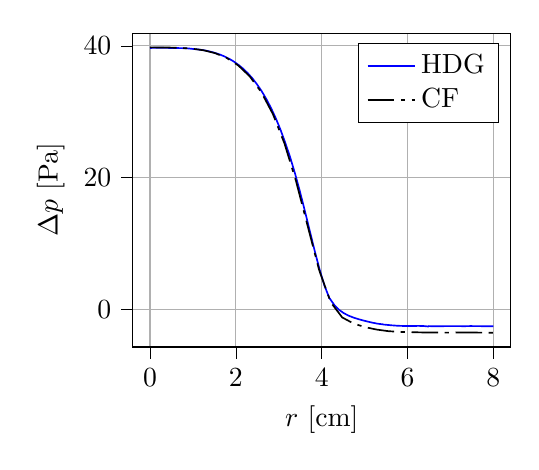
\begin{tikzpicture}

\definecolor{darkgray176}{RGB}{176,176,176}

\begin{axis}[
legend cell align=left,
legend pos= north east,
scale = .7,
ylabel = {$\Delta p$ [Pa]},
tick align=outside,
tick pos=left,
x grid style={darkgray176},
xmajorgrids,
xlabel = {$r$ [cm]},
xmin=-0.399999991059303, xmax=8.39999981224537,
xtick style={color=black},
y grid style={darkgray176},
ymajorgrids,
ymin=-5.6948538724031, ymax=41.9224724193336,
ytick style={color=black}
]
\addplot [semithick, blue]
table {%
0 39.6688072292245
0.007999999797903 39.6713430838637
0.015999999595806 39.6738789384645
0.023999999393709 39.6764147930269
0.031999999191612 39.6789506475509
0.039999998989515 39.6814865020364
0.047999998787418 39.6840223564836
0.0560000014957041 39.6865582118149
0.063999998383224 39.6890940652627
0.0720000010915101 39.6916299205172
0.07999999797903 39.6941657738881
0.0880000006873161 39.6967016290658
0.095999997574836 39.6992374823599
0.104000000283122 39.7010468236692
0.112000002991408 39.7013744070808
0.119999994058162 39.7017019900096
0.127999996766448 39.7020295734089
0.135999999474734 39.7023571568021
0.14400000218302 39.7026847401893
0.151999993249774 39.7030123230936
0.15999999595806 39.7033399064684
0.167999998666346 39.7036674898372
0.176000001374632 39.7039950731998
0.183999992441386 39.7043226560796
0.191999995149672 39.70465023943
0.199999986216426 39.7049778222976
0.208000000566244 39.7045987524011
0.215999991632998 39.7038523867544
0.224000005982816 39.7031060189444
0.23199999704957 39.7023596533157
0.239999988116324 39.7016132876959
0.248000002466142 39.7008669199129
0.255999993532896 39.7001205543111
0.26399998459965 39.6993741887183
0.271999998949468 39.6986278209623
0.279999990016222 39.6978814553875
0.28800000436604 39.6971350876494
0.295999995432794 39.6963887220925
0.303999986499548 39.6956423565447
0.312000000849366 39.6946049542731
0.31999999191612 39.6935637191702
0.327999982982874 39.6925224840817
0.335999997332692 39.6914812459772
0.343999988399446 39.6904400109176
0.352000002749264 39.6893987728419
0.359999993816018 39.6883575378111
0.367999984882772 39.6873163027948
0.37599999923259 39.6862750647624
0.383999990299344 39.6852338297749
0.392000004649162 39.6841925917714
0.399999972432852 39.6831513598432
0.40799998678267 39.682150874789
0.416000001132488 39.6812386061571
0.423999968916178 39.680326342853
0.431999983265996 39.6794140742565
0.439999997615814 39.6785018056779
0.448000011965632 39.677589537117
0.455999979749322 39.676677273884
0.46399999409914 39.6757650053587
0.472000008448958 39.6748527368511
0.479999976232648 39.6739404736713
0.487999990582466 39.6730282051993
0.496000004932284 39.672115936745
0.503999972715974 39.6712036736186
0.511999987065792 39.6704188329088
0.52000000141561 39.6697041302054
0.5279999691993 39.6689894316887
0.535999983549118 39.6682747290384
0.543999997898936 39.6675600264147
0.551999965682626 39.6668453279776
0.559999980032444 39.6661306254069
0.567999994382262 39.6654159228627
0.57600000873208 39.6647012203451
0.58399997651577 39.6639865220142
0.591999990865588 39.6632718195496
0.600000005215406 39.6625571171116
0.607999972999096 39.6618424188603
0.615999987348914 39.6610409554736
0.624000001698732 39.6602371750612
0.631999969482422 39.6594333993758
0.63999998383224 39.6586296190602
0.647999998182058 39.6578258387929
0.655999965965748 39.6570220632525
0.663999980315566 39.656218283082
0.671999994665384 39.6554145029597
0.679999962449074 39.6546107275645
0.687999976798892 39.653806947539
0.69599999114871 39.6530031675619
0.704000005498528 39.6521993876331
0.711999973282218 39.6511741390321
0.719999987632036 39.6496393952062
0.728000001981854 39.6481046514712
0.735999969765544 39.6465699167603
0.743999984115362 39.6450351732067
0.75199999846518 39.643500429744
0.75999996624887 39.6419656953054
0.767999980598688 39.6404309520242
0.775999994948506 39.6388962088337
0.784000009298325 39.6373614657341
0.791999977082014 39.6358267316586
0.799999944865704 39.6342919976739
0.808000005781651 39.6327572459133
0.81599997356534 39.6301303778759
0.82399994134903 39.6268675625544
0.832000002264977 39.6236047094099
0.839999970048666 39.6203418944112
0.847999937832355 39.6170790795738
0.855999998748302 39.6138162269135
0.863999966531992 39.6105534123989
0.871999934315681 39.6072905980457
0.879999995231628 39.6040277458696
0.887999963015318 39.6007649318392
0.896000023931265 39.5975020799859
0.903999991714954 39.5942392662783
0.911999959498644 39.5909764527321
0.920000020414591 39.5847532900981
0.92799998819828 39.5784100356403
0.93599995598197 39.5720667814506
0.944000016897917 39.5657234536833
0.951999984681606 39.5593802000295
0.959999952465296 39.5530369466438
0.968000013381243 39.5466936196806
0.975999981164932 39.5403503668309
0.983999948948622 39.5340071142492
0.992000009864569 39.5276637880902
0.999999977648258 39.5213205360446
1.00799994543195 39.5149772842672
1.01600000634789 39.5131354788737
1.02399997413158 39.5085406983426
1.03199994191527 39.503945918385
1.04000000283122 39.4993510855105
1.04799997061491 39.4947563066998
1.0559999383986 39.4901615284622
1.06399999931455 39.4855666973078
1.07199996709824 39.4809719202166
1.07999993488193 39.476377143698
1.08799999579787 39.471782314263
1.09599996358156 39.4671875388905
1.10399993136525 39.4625927640907
1.1119999922812 39.457997936373
1.11999996006489 39.45275716161
1.12800002098083 39.4456083577859
1.13599998876452 39.4384596389355
1.14399995654821 39.4313109218362
1.15200001746416 39.4241621232653
1.15999998524785 39.4170134096667
1.16799995303154 39.4098646978191
1.17600001394749 39.4027159044983
1.18399998173118 39.3955671961488
1.19199994951487 39.3884184895499
1.20000001043081 39.3812697014768
1.2079999782145 39.3741209983744
1.21599994599819 39.3669722970201
1.22400000691414 39.3592870370373
1.23199997469783 39.3496536320061
1.23999994248152 39.3400202296137
1.24800000339746 39.3303867177115
1.25599997118115 39.3207533205952
1.26399993896484 39.3111199261156
1.27199999988079 39.301486422126
1.27999996766448 39.29185303292
1.28799993544817 39.2822196463492
1.29599999636412 39.2725861502678
1.30399996414781 39.2629527689681
1.3119999319315 39.2533193903028
1.31999999284744 39.2436859021237
1.32799996063113 39.2335945007374
1.33599992841482 39.2214006717655
1.34399998933077 39.2092067042247
1.35199995711446 39.1970128820249
1.35999992489815 39.1848190632103
1.36799998581409 39.1726251058242
1.37599995359778 39.1604312937786
1.38400001451373 39.1482373431603
1.39199998229742 39.1360435378791
1.39999995008111 39.1238497359819
1.40800001099706 39.1116557955099
1.41599997878075 39.0994620003738
1.42399994656444 39.0872682086178
1.43200000748038 39.0746796651943
1.43999997526407 39.0597046834374
1.44799994304776 39.0447297058238
1.45600000396371 39.0297545580204
1.4639999717474 39.014779588691
1.47199993953109 38.9998046235018
1.48000000044703 38.9848294881223
1.48799996823072 38.9698545312136
1.49599993601441 38.9548795784426
1.50399999693036 38.9399044554799
1.51199996471405 38.9249295109852
1.51999993249774 38.909954570627
1.52799999341369 38.8949794600725
1.53599996119738 38.879674447528
1.54399992898107 38.861552593876
1.55199998989701 38.8434305343153
1.5599999576807 38.8253086907786
1.56800001859665 38.8071866413315
1.57599989324808 38.7890650188722
1.58399995416403 38.770942979536
1.59200001507998 38.7528209452522
1.59999988973141 38.7346993379532
1.60799995064735 38.7165773137753
1.6160000115633 38.6984552946469
1.62399988621473 38.6803337025011
1.63199994713068 38.6622116934715
1.64000000804663 38.6438412554814
1.64799988269806 38.6220620870976
1.65599994361401 38.6002824178982
1.66400000452995 38.5785027549761
1.67199987918139 38.5567236054232
1.67999994009733 38.5349439550505
1.68800000101328 38.5131643109541
1.69599987566471 38.4913851802218
1.70399993658066 38.4696055486668
1.7119999974966 38.447825923385
1.71999987214804 38.4260468114631
1.72799993306398 38.4042671987169
1.73599999397993 38.3824875922374
1.74399986863136 38.3605750163122
1.75199992954731 38.3344820468967
1.75999999046326 38.3083890854295
1.7680000513792 38.2822961319089
1.77599992603064 38.2562037938526
1.78399998694658 38.2301108562192
1.79200004786253 38.2040179265313
1.79999992251396 38.1779256123013
1.80799998342991 38.1518326984906
1.81600004434586 38.1257397926211
1.82399991899729 38.0996475022043
1.83199997991323 38.0735546122046
1.84000004082918 38.0474617301385
1.84799991548061 38.021369463522
1.85599997639656 37.9901931774938
1.86400003731251 37.9589862688871
1.87199991196394 37.927780097083
1.87999997287989 37.8965732089064
1.88800003379583 37.8653663309403
1.89599990844727 37.8341601897744
1.90399996936321 37.8029533322294
1.91200003027916 37.7717464848894
1.91999990493059 37.7405403743432
1.92799996584654 37.7093335474129
1.93600002676249 37.6781267306838
1.94399990141392 37.6469206507386
1.95199996232986 37.6157138544062
1.96000002324581 37.5787073847844
1.96799989789724 37.5414417705577
1.97599995881319 37.5041753018848
1.98400001972914 37.4669088464345
1.99199989438057 37.4296432718723
1.99999995529652 37.392376842862
2.00800001621246 37.3551104270653
2.0159998908639 37.3178448921488
2.02399995177984 37.2805785027774
2.03200001269579 37.2433121266122
2.03999988734722 37.2060466313212
2.04799994826317 37.168780281565
2.05600000917912 37.1315139450098
2.06399988383055 37.0896790086362
2.07199994474649 37.0473265930439
2.08000000566244 37.0049741499038
2.08799988031387 36.9626226653275
2.09599994122982 36.9202701671628
2.10400000214577 36.877917641521
2.1119998767972 36.835566074515
2.11999993771315 36.7932134939899
2.12799999862909 36.7508608860576
2.13599987328053 36.7085092368337
2.14399993419647 36.6661565741584
2.15199999511242 36.6238038841462
2.15999986976385 36.5814521529145
2.1679999306798 36.5368832425401
2.17599999159575 36.4868688597293
2.18399986624718 36.4368555985999
2.19199992716312 36.3868411302278
2.19999998807907 36.3368266191291
2.2079998627305 36.286813229824
2.21599992364645 36.2367986333724
2.2239999845624 36.1867839943152
2.23199985921383 36.1367704771696
2.23999992012978 36.0867557529853
2.24799998104572 36.0367409862921
2.25600004196167 35.9867261771262
2.2639999166131 35.9367124900143
2.27199997752905 35.8866975960123
2.280000038445 35.8312551040247
2.28799991309643 35.7729961298947
2.29599997401237 35.7147357443551
2.30400003492832 35.6564753039207
2.31199990957975 35.5982161651113
2.3199999704957 35.5399556150282
2.32800003141165 35.4816950101888
2.33599990606308 35.4234357071196
2.34399996697903 35.3651749929113
2.35200002789497 35.3069142240867
2.35999990254641 35.2486547571731
2.36799996346235 35.1903938792563
2.3760000243783 35.1321329468619
2.38399989902973 35.0736304989037
2.39199995994568 35.006423228402
2.40000002086163 34.939215892548
2.40799989551306 34.8720100561801
2.415999956429 34.8048025897887
2.42400001734495 34.7375950582105
2.43199989199638 34.6703890262884
2.43999995291233 34.6031813645014
2.44800001382828 34.5359736376969
2.45599988847971 34.4687674107156
2.46399994939566 34.4015595540318
2.4720000103116 34.3343516324907
2.47999988496304 34.2671452109438
2.48799994587898 34.1999371598538
2.49600000679493 34.1288627990237
2.50399988144636 34.0518921486561
2.51199994236231 33.9749196310072
2.52000000327826 33.8979470382801
2.52799987792969 33.8209761626847
2.53599993884563 33.7440034199924
2.54399999976158 33.667030602402
2.55199987441301 33.5900595021386
2.55999993532896 33.5130865349884
2.56799999624491 33.4361134931204
2.57599987089634 33.3591421687724
2.58399993181229 33.2821689776945
2.59199999272823 33.2051957121047
2.59999986737967 33.1282241642281
2.60799992829561 33.0430692672188
2.61599998921156 32.9553962760646
2.62399986386299 32.8677252406112
2.63199992477894 32.7800520783658
2.63999998569489 32.6923788306815
2.64799986034632 32.6047075389191
2.65599992126226 32.5170341205735
2.66399998217821 32.4293606170039
2.67199985682964 32.3416890695765
2.67999991774559 32.2540153957743
2.68799997866154 32.1663416369618
2.69599985331297 32.0786698345112
2.70399991422892 31.9909959058934
2.71199997514486 31.9017554093331
2.7199998497963 31.8023316927061
2.72799991071224 31.7029055632774
2.73599997162819 31.6034793360529
2.74399984627962 31.5040553260472
2.75199990719557 31.4046289034783
2.75999996811152 31.3052023833274
2.76800002902746 31.2057757657623
2.77599990367889 31.1063513657335
2.78399996459484 31.0069245534513
2.79200002551079 30.9074976439434
2.79999990016222 30.8080729522397
2.80799996107817 30.7086458485258
2.81600002199411 30.6092186478292
2.82399989664555 30.5033093581476
2.83199995756149 30.390960340585
2.84000001847744 30.2786112099969
2.84799989312887 30.1662645822935
2.85599995404482 30.0539152259392
2.86400001496077 29.9415657568413
2.8719998896122 29.8292187909104
2.87999995052814 29.7168690965817
2.88800001144409 29.6045192898533
2.89599988609552 29.4921719865527
2.90399994701147 29.3798219551474
2.91200000792742 29.2674718115597
2.91999988257885 29.1551241717225
2.9279999434948 29.0427738040523
2.93600000441074 28.9180579591851
2.94399987906218 28.7915017761771
2.95199993997812 28.6649425143786
2.96000000089407 28.5383831205597
2.9679998755455 28.4118265415024
2.97599993646145 28.2852668839739
2.9839999973774 28.1587070947527
2.99199987202883 28.0321501206305
2.99999993294477 27.9055900683549
3.00799999386072 27.7790298847138
3.01599986851215 27.652472516507
3.0239999294281 27.5259120704642
3.03199999034405 27.3993514933817
3.03999986499548 27.2690681236519
3.04799992591143 27.1268945422765
3.05599998682737 26.9847208044925
3.06399986147881 26.8425502206498
3.07199992239475 26.7003761704399
3.0799999833107 26.5582019642089
3.08799985796213 26.4160309122862
3.09599991887808 26.273856394417
3.10399997979403 26.1316817209149
3.11199985444546 25.9895102021318
3.1199999153614 25.8473352177316
3.12799997627735 25.7051600780811
3.1360000371933 25.5629847833081
3.14400009810925 25.4208093335407
3.15199978649616 25.2675745791318
3.15999984741211 25.1138343705221
3.16799990832806 24.9600941786072
3.175999969244 24.8063540033346
3.18400003015995 24.652613844652
3.1920000910759 24.4988737025075
3.19999977946281 24.3451407358766
3.20799984037876 24.1914006266519
3.21599990129471 24.0376605338103
3.22399996221066 23.8839204573005
3.2320000231266 23.7301803970717
3.24000008404255 23.576440353073
3.24799977242947 23.4227074842768
3.25599983334541 23.2689674725861
3.26399989426136 23.1094177243608
3.27199995517731 22.9362281392879
3.28000001609325 22.7630385807091
3.2880000770092 22.5898490485423
3.29599976539612 22.4166676074084
3.30399982631207 22.2434781278192
3.31199988722801 22.0702886743977
3.31999994814396 21.8970992470547
3.32800000905991 21.7239098457347
3.33600006997585 21.5507204703328
3.34399975836277 21.377539185473
3.35199981927872 21.2043498616835
3.35999988019466 21.031160563582
3.36799994111061 20.8579712910896
3.37600000202656 20.684782044128
3.3840000629425 20.4939927082318
3.39199975132942 20.3030435906571
3.39999981224537 20.112085605265
3.40799987316132 19.9211276440894
3.41599993407726 19.7301697070564
3.42399999499321 19.5392117940926
3.43200005590916 19.3482539051131
3.43999974429607 19.1573049321799
3.44799980521202 18.9663470909841
3.45599986612797 18.7753892735663
3.46399992704391 18.5844314798544
3.47199998795986 18.3934737097766
3.48000004887581 18.2025159632615
3.48799973726273 18.0115671323314
3.49599979817867 17.8112164969727
3.50399985909462 17.6064909680938
3.51199992001057 17.4017654532689
3.51999998092651 17.1970399524557
3.52800004184246 16.992314465612
3.53600010275841 16.787588992696
3.54399979114532 16.5828730668649
3.55199985206127 16.3781476216783
3.55999991297722 16.1734221902944
3.56799997389317 15.968696772672
3.57600003480911 15.76397136877
3.58400009572506 15.5592459785474
3.59199978411198 15.3545301351587
3.59999984502792 15.149804772172
3.60799990594387 14.9422944121656
3.61599996685982 14.7301224239008
3.62400002777576 14.5179504347634
3.63200008869171 14.3057784447558
3.63999977707863 14.0936163338337
3.64799983799458 13.8814443420936
3.65599989891052 13.6692723494911
3.66399995982647 13.4571003560288
3.67200002074242 13.2449283617091
3.68000008165836 13.0327563665346
3.68799977004528 12.8205942504612
3.69599983096123 12.6084222535847
3.70399989187717 12.396250255861
3.71199995279312 12.1840782572925
3.72000001370907 11.9719848011441
3.72800007462502 11.7610076359423
3.73599976301193 11.5500402775672
3.74399982392788 11.3390630774383
3.75199988484383 11.1280858599219
3.75999994575977 10.9171086250688
3.76800000667572 10.7061313729297
3.77600006759167 10.4951541035515
3.78399975597858 10.2841866413159
3.79199981689453 10.073209337621
3.79999987781048 9.86223201684057
3.80799993872643 9.65125467902409
3.81599999964237 9.44027732422106
3.82400006055832 9.22929995248067
3.83199974894524 9.01833238817782
3.83999980986118 8.81656256838975
3.84799987077713 8.61774179805197
3.85599993169308 8.4189209946664
3.86399999260902 8.22010015832846
3.87200005352497 8.02127928913306
3.87999974191189 7.82246764542482
3.88799980282784 7.62364671079952
3.89599986374378 7.42482574359947
3.90399992465973 7.22600474391822
3.91199998557568 7.02718371184895
3.92000004649162 6.82836264748444
3.92799973487854 6.62955080917618
3.93599979579449 6.43072968049967
3.94399985671043 6.23190851980427
3.95199991762638 6.04451230709813
3.95999997854233 5.87112994094036
3.96800003945827 5.69774752949685
3.97599972784519 5.52437314658584
3.98399978876114 5.35099064495911
3.99199984967709 5.17760809843181
3.99999991059303 5.00422550713146
4.00799997150898 4.83084287118498
4.01600003242493 4.65746019071885
4.02400009334087 4.48407746585909
4.03199978172779 4.31070277043512
4.03999984264374 4.13731995716626
4.04799990355968 3.96393709987889
4.05599996447563 3.79055419869719
4.06400002539158 3.62295009098701
4.07200008630753 3.49060865200997
4.07999977469444 3.35827332347406
4.08799983561039 3.22593178035778
4.09599989652634 3.09359018538982
4.10399995744228 2.9612485387156
4.11200001835823 2.82890684047991
4.12000007927418 2.69656509082706
4.12799976766109 2.56422945250051
4.13599982857704 2.43188760044652
4.14399988949299 2.29954569740508
4.15199995040894 2.16720374351836
4.16000001132488 2.03486173892793
4.16800007224083 1.90251968377498
4.17599976062775 1.7701837408138
4.18399982154369 1.68692557741597
4.19199988245964 1.61354804652919
4.19999994337559 1.54017046411465
4.20800000429153 1.46679283031511
4.21600006520748 1.39341514527277
4.2239997535944 1.3200408260216
4.23199981451035 1.2466630389206
4.23999987542629 1.17328520100029
4.24799993634224 1.09990731240082
4.25599999725819 1.02652937326181
4.26400005817413 0.953151383722364
4.27199974656105 0.879776760827462
4.279999807477 0.806398670904739
4.28799986839294 0.73302053099583
4.29599992930889 0.62190922268862
4.30399999022484 0.571499026352933
4.31200005114079 0.521088918808404
4.3199997395277 0.470681247679398
4.32799980044365 0.420271318448653
4.3359998613596 0.369861478746513
4.34399992227554 0.319451728820598
4.35199998319149 0.269042068919468
4.36000004410744 0.218632499292586
4.36799973249435 0.168225367544648
4.3759997934103 0.117815979214123
4.38399985432625 0.0674066819117934
4.3919999152422 0.0169974758908314
4.39999997615814 -0.0334116385946236
4.40800003707409 -0.078870911400393
4.41599972546101 -0.115287518499137
4.42399978637695 -0.151705767138195
4.4319998472929 -0.188123961318079
4.43999990820885 -0.224542100886485
4.44799996912479 -0.260960185690509
4.45600003004074 -0.2973782155767
4.46399971842766 -0.333794494561116
4.47199977934361 -0.37021241415154
4.47999984025955 -0.406630278360301
4.4879999011755 -0.443048087031636
4.49599996209145 -0.479465840009183
4.50400002300739 -0.515883537135996
4.51200008392334 -0.552301178254555
4.51999977231026 -0.58692330852874
4.5279998332262 -0.613567558654591
4.53599989414215 -0.640211779799376
4.5439999550581 -0.666855971881044
4.55200001597404 -0.693500134817228
4.56000007688999 -0.720144268525255
4.56799976527691 -0.746787132219472
4.57599982619286 -0.773431207221995
4.5839998871088 -0.800075252749001
4.59199994802475 -0.82671926871273
4.6000000089407 -0.8533632550302
4.60800006985664 -0.880007211616833
4.61599975824356 -0.90664989769335
4.62399981915951 -0.933293794564681
4.63199988007545 -0.959937661449512
4.6399999409914 -0.980105275291389
4.64800000190735 -1.00035867244938
4.6560000628233 -1.02061205768528
4.66399975121021 -1.04086448785115
4.67199981212616 -1.06111784914061
4.67999987304211 -1.08137119840488
4.68799993395805 -1.10162453560877
4.695999994874 -1.12187786071918
4.70400005578995 -1.14213117369953
4.71199974417686 -1.162383531405
4.71999980509281 -1.18263682002169
4.72799986600876 -1.20289009640335
4.73599992692471 -1.22314336051456
4.74399998784065 -1.24339661231973
4.7520000487566 -1.26040941473119
4.75999973714352 -1.27681983697016
4.76799979805946 -1.29323102142289
4.77599985897541 -1.30964220388393
4.78399991989136 -1.32605338434748
4.7919999808073 -1.34246456280772
4.80000004172325 -1.35887573925881
4.80799973011017 -1.37528614949587
4.81599979102612 -1.39169732191109
4.82399985194206 -1.40810849229947
4.83199991285801 -1.42451966065506
4.83999997377396 -1.44093082697191
4.8480000346899 -1.45734199124402
4.85599972307682 -1.47375238926697
4.86399978399277 -1.48873034805885
4.87199984490871 -1.50301338711704
4.87999990582466 -1.51729642810731
4.88799996674061 -1.53157947103537
4.89600002765656 -1.54586251590694
4.90399971604347 -1.56014489762658
4.91199977695942 -1.57442794640234
4.91999983787537 -1.58871099713892
4.92799989879131 -1.60299404984213
4.93599995970726 -1.61727710451781
4.94400002062321 -1.63156016117183
4.95199970901012 -1.64584255470834
4.95999976992607 -1.6601256153366
4.96799983084202 -1.67440867796093
4.97599989175797 -1.68806286795118
4.98399995267391 -1.70109731703796
4.99200001358986 -1.71413176729699
4.99999970197678 -1.72716561177243
5.00799976289272 -1.74020006438644
5.01599982380867 -1.75323451818326
5.02399988472462 -1.76626897316644
5.03199994564056 -1.77930342933955
5.04000000655651 -1.79233788670616
5.04800006747246 -1.80537234526988
5.05599975585938 -1.81840619807456
5.06399981677532 -1.83144065904325
5.07199987769127 -1.8444751212199
5.07999993860722 -1.85750958460817
5.08799999952316 -1.8701421162343
5.09600006043911 -1.88197307222892
5.10399974882603 -1.89380347454933
5.11199980974197 -1.90563442502215
5.11999987065792 -1.91746537272143
5.12799993157387 -1.92929631763873
5.13599999248981 -1.94112725976559
5.14400005340576 -1.9529581990935
5.15199974179268 -1.96478858469726
5.15999980270863 -1.97661951840176
5.16799986362457 -1.98845044928158
5.17599992454052 -2.0002813773281
5.18399998545647 -2.01211230253263
5.19200004637241 -2.02394322488646
5.19999973475933 -2.03544608330883
5.20799979567528 -2.04528423315753
5.21599985659122 -2.05512237484983
5.22399991750717 -2.06496050836062
5.23199997842312 -2.0747986336647
5.24000003933907 -2.08463675073673
5.24799972772598 -2.09447440143236
5.25599978864193 -2.10431250196386
5.26399984955788 -2.11415059418772
5.27199991047382 -2.12398867807674
5.27999997138977 -2.13382675360558
5.28800003230572 -2.14366482074827
5.29599972069263 -2.15350242136214
5.30399978160858 -2.16334047165466
5.31199984252453 -2.17317851348254
5.31999990344048 -2.17941863030469
5.32799996435642 -2.18564029136006
5.33600002527237 -2.19186193925667
5.34399971365929 -2.19808328423843
5.35199977457523 -2.20430490569452
5.35999983549118 -2.21052651386789
5.36799989640713 -2.21674810871642
5.37599995732307 -2.22296969019968
5.38400001823902 -2.22919125827424
5.39199970662594 -2.2354125231872
5.39999976754189 -2.24163406431921
5.40799982845783 -2.2478555919159
5.41599988937378 -2.25407710593456
5.42399995028973 -2.26029860633227
5.43200001120567 -2.28775724226172
5.43999969959259 -2.29269342403873
5.44799976050854 -2.2976298287667
5.45599982142448 -2.30256622657155
5.46399988234043 -2.30750261744716
5.47199994325638 -2.31243900138741
5.48000000417233 -2.31737537838615
5.48799969255924 -2.3223115185716
5.49599975347519 -2.32724788166931
5.50399981439114 -2.33218423780712
5.51199987530708 -2.33712058697886
5.51999993622303 -2.34205692917838
5.52799999713898 -2.34699326439951
5.53600005805492 -2.35187670170757
5.54399974644184 -2.35672021788019
5.55199980735779 -2.3615639585157
5.55999986827374 -2.36640769806055
5.56799992918968 -2.37125143651375
5.57599999010563 -2.37609517387435
5.58400005102158 -2.38093891014136
5.59199973940849 -2.38578241976158
5.59999980032444 -2.39062615383859
5.60799986124039 -2.3954698868191
5.61599992215633 -2.40031361870216
5.62399998307228 -2.40515734948677
5.63200004398823 -2.41000107917197
5.63999973237514 -2.414553625969
5.64799979329109 -2.41847931299973
5.65599985420704 -2.42240500148789
5.66399991512299 -2.42633069143479
5.67199997603893 -2.4302563828417
5.68000003695488 -2.43418207570994
5.6879997253418 -2.43810758723775
5.69599978625774 -2.44203328303238
5.70399984717369 -2.44595898029246
5.71199990808964 -2.44988467901895
5.71999996900558 -2.45381037921329
5.72800002992153 -2.45773608087678
5.73599971830845 -2.46166160120729
5.7439997792244 -2.46550109159008
5.75199984014034 -2.46805047041044
5.75999990105629 -2.47059985085865
5.76799996197224 -2.47314923293616
5.77600002288818 -2.47569861664444
5.7839997112751 -2.4782478832708
5.79199977219105 -2.48079727024497
5.79999983310699 -2.48334665885418
5.80799989402294 -2.48589604909998
5.81599995493889 -2.48844544098388
5.82400001585484 -2.49099483450732
5.83199970424175 -2.49354411095715
5.8399997651577 -2.49609350776397
5.84799982607365 -2.49864290621472
5.85599988698959 -2.50000610418873
5.86399994790554 -2.50108808190816
5.87200000882149 -2.50217005998534
5.8799996972084 -2.50325198803743
5.88799975812435 -2.50433396683108
5.8959998190403 -2.50541594598345
5.90399987995625 -2.50649792549488
5.91199994087219 -2.50757990536563
5.92000000178814 -2.5086618855961
5.92799969017506 -2.5097438158033
5.935999751091 -2.5108257967541
5.94399981200695 -2.51190777806555
5.9519998729229 -2.51298975973799
5.95999993383884 -2.51341165887248
5.96799999475479 -2.51330233176526
5.97599968314171 -2.51319300836322
5.98399974405766 -2.51308367848317
5.9919998049736 -2.51297434721479
5.99999986588955 -2.51286501455684
6.0079999268055 -2.51275568050806
6.01599998772144 -2.5126463450672
6.02400004863739 -2.51253700823301
6.03199973702431 -2.51242767509567
6.03999979794025 -2.5123183354711
6.0479998588562 -2.51220899444943
6.05599991977215 -2.51209965202938
6.0639999806881 -2.51182602160042
6.07200004160404 -2.5111687129103
6.07999972999096 -2.51051143223171
6.08799979090691 -2.50985411834589
6.09599985182285 -2.50919680185864
6.1039999127388 -2.50853948276761
6.11199997365475 -2.50788216107061
6.12000003457069 -2.50722483676548
6.12799972295761 -2.50656754045727
6.13599978387356 -2.50591021092766
6.14399984478951 -2.50525287878246
6.15199990570545 -2.50459554401931
6.1599999666214 -2.50393820663583
6.16800002753735 -2.50330194102863
6.17599971592426 -2.50310724107669
6.18399977684021 -2.50291252982334
6.19199983775616 -2.50271781633329
6.1999998986721 -2.50252310060449
6.20799995958805 -2.50232838263492
6.216000020504 -2.50213366242304
6.22399970889091 -2.50193894903305
6.23199976980686 -2.5017442243288
6.23999983072281 -2.50154949737588
6.24799989163876 -2.50135476817199
6.2559999525547 -2.50116003671509
6.26399964094162 -2.5009653120711
6.2720000743866 -2.50077056703404
6.27999976277351 -2.50203213956507
6.28800019621849 -2.50367798050204
6.29599988460541 -2.50532366894466
6.30399957299232 -2.50696935816617
6.3120000064373 -2.50861520144011
6.31999969482422 -2.51026089222161
6.3280001282692 -2.51190673705714
6.33599981665611 -2.51355242940146
6.34399950504303 -2.51519812252825
6.35199993848801 -2.5168439697114
6.35999962687492 -2.51848966440531
6.3680000603199 -2.52013551315715
6.37599974870682 -2.52178120942105
6.38400018215179 -2.5253527527011
6.39199987053871 -2.53058395130322
6.39999955892563 -2.53581515746679
6.40799999237061 -2.54104685841278
6.41599968075752 -2.54627807972068
6.4240001142025 -2.55150979582627
6.43199980258942 -2.55674103230624
6.43999949097633 -2.56197227638231
6.44799992442131 -2.56720401527905
6.45599961280823 -2.57243527456892
6.4640000462532 -2.57766702869481
6.47199973464012 -2.58289830322637
6.4800001680851 -2.58813007260936
6.48799985647202 -2.52844084491245
6.49599954485893 -2.53043115131971
6.50399997830391 -2.53242165908309
6.51199966669083 -2.53441199746404
6.5200001001358 -2.53640253720877
6.52799978852272 -2.53839290757276
6.5360002219677 -2.54038347930815
6.54399991035461 -2.54237388166448
6.55199959874153 -2.54436430001974
6.56000003218651 -2.54635491975787
6.56799972057343 -2.54834537011949
6.5760001540184 -2.55033602187162
6.58399984240532 -2.55232650424891
6.59199953079224 -2.55319878527119
6.59999996423721 -2.55333911085991
6.60799965262413 -2.55347942087517
6.61600008606911 -2.55361974145244
6.62399977445602 -2.55376004645588
6.632000207901 -2.55390036202008
6.63999989628792 -2.5540406620103
6.64799958467484 -2.55418095949349
6.65600001811981 -2.55432126753566
6.66399970650673 -2.55446156000344
6.67200013995171 -2.55460186302884
6.67999982833862 -2.55474215047967
6.68799951672554 -2.55488243542162
6.69599995017052 -2.55425152186408
6.70399963855743 -2.55355903979944
6.71200007200241 -2.55286648306108
6.71999976038933 -2.55217398063886
6.7280001938343 -2.55148140353793
6.73599988222122 -2.55078888075234
6.74399957060814 -2.55009634778332
6.75200000405312 -2.54940374012827
6.75999969244003 -2.54871118678695
6.76800012588501 -2.54801855875474
6.77599981427193 -2.54732598503488
6.78399950265884 -2.5466334011243
6.79199993610382 -2.5459158923648
6.79999962449074 -2.54512297866052
6.80800005793571 -2.5443299809908
6.81599974632263 -2.54353704705363
6.82400017976761 -2.54274402914596
6.83199986815453 -2.54195107496967
6.83999955654144 -2.54115811067219
6.84799998998642 -2.54036506239721
6.85599967837334 -2.53957207785198
6.86400011181831 -2.53877900932441
6.87199980020523 -2.5379860045253
6.87999948859215 -2.53719298959771
6.88799992203712 -2.53639989068046
6.89599961042404 -2.53580448440481
6.90400004386902 -2.53535848541286
6.91199973225594 -2.53491252252949
6.92000016570091 -2.53446651268369
6.92799985408783 -2.53402053894573
6.93599954247475 -2.53357455977959
6.94399997591972 -2.53312853364706
6.95199966430664 -2.53268254362168
6.96000009775162 -2.53223650662731
6.96799978613853 -2.53179050573953
6.97599947452545 -2.53134449941937
6.98399990797043 -2.53089844612642
6.99199959635735 -2.53045242893917
7.00000002980232 -2.53046029994235
7.00799971818924 -2.53052364585087
7.01600015163422 -2.53058699843083
7.02399984002113 -2.53065034588234
7.03199952840805 -2.53071369410554
7.03999996185303 -2.53077704900063
7.04799965023994 -2.53084039876759
7.05600008368492 -2.53090375520682
7.06399977207184 -2.53096710651801
7.07200020551682 -2.53103046450183
7.07999989390373 -2.53109381735749
7.08799958229065 -2.53115717098572
7.09600001573563 -2.53130280343069
7.10399970412254 -2.53175264009444
7.11200013756752 -2.53220252399122
7.11999982595444 -2.53265237132901
7.12799951434135 -2.5331022240046
7.13599994778633 -2.53355212391706
7.14399963617325 -2.53400198727133
7.15200006961823 -2.53445189786503
7.15999975800514 -2.53490177190111
7.16800019145012 -2.53535169317919
7.17599987983704 -2.53580157790009
7.18399956822395 -2.53625146796444
7.19200000166893 -2.5367014052746
7.19999969005585 -2.53713973731
7.20800012350082 -2.53756804317656
7.21599981188774 -2.53799631427124
7.22399950027466 -2.53842459048157
7.23199993371964 -2.53885291169673
7.23999962210655 -2.53928119814086
7.24800005555153 -2.53970952959237
7.25599974393845 -2.54013782627341
7.26400017738342 -2.54056616796428
7.27199986577034 -2.54099447488522
7.27999955415726 -2.54142278692686
7.28799998760223 -2.54185114398209
7.29599967598915 -2.54227946626818
7.30400010943413 -2.54209543572747
7.31199979782104 -2.54180870866972
7.31999948620796 -2.54152197854243
7.32799991965294 -2.54123521863948
7.33599960803986 -2.54094848237098
7.34400004148483 -2.5406617163256
7.35199972987175 -2.54037497391434
7.36000016331673 -2.54008820172472
7.36799985170364 -2.53980145316889
7.37599954009056 -2.53951470154024
7.38399997353554 -2.53922792013079
7.39199966192245 -2.53894116235476
7.40000009536743 -2.53835253094322
7.40799978375435 -2.53637194474502
7.41599947214127 -2.53439133614021
7.42399990558624 -2.53241052065686
7.43199959397316 -2.53042986722678
7.44000002741814 -2.52844900690723
7.44799971580505 -2.52646830863893
7.45600014925003 -2.52448740347042
7.46399983763695 -2.52250666035076
7.47199952602386 -2.52052589480153
7.47999995946884 -2.51854492233563
7.48799964785576 -2.51656411191512
7.49600008130074 -2.51458309456745
7.50399976968765 -2.5265335425756
7.51200020313263 -2.52860782998487
7.51999989151955 -2.53017044181924
7.52799957990646 -2.53101698492865
7.53600001335144 -2.53165066855198
7.54399970173836 -2.53185842555216
7.55200013518333 -2.53201658269205
7.55999982357025 -2.53202588399755
7.56799951195717 -2.53205075319467
7.57599994540215 -2.53215350221524
7.58399963378906 -2.53227597299995
7.59200006723404 -2.53261563980191
7.59999975562096 -2.53295527497165
7.60800018906593 -2.53352687345177
7.61599987745285 -2.53409842578459
7.62399956583977 -2.53474193770585
7.63199999928474 -2.53539205357695
7.63999968767166 -2.5358559864747
7.64800012111664 -2.53628273297587
7.65599980950356 -2.53620420978223
7.66399949789047 -2.53595728145608
7.67199993133545 -2.53739276692333
7.67999961972237 -2.53776410690329
7.68800005316734 -2.53820710505604
7.69599974155426 -2.53870122206011
7.70400017499924 -2.53922516826441
7.71199986338615 -2.53977884670291
7.71999955177307 -2.54033722298831
7.72799998521805 -2.54090222996527
7.73599967360497 -2.54145982471632
7.74400010704994 -2.54200274899659
7.75199979543686 -2.54253549683642
7.75999948382378 -2.54303786447263
7.76799991726875 -2.5435329454736
7.77599960565567 -2.54399131144126
7.78400003910065 -2.54444700581916
7.79199972748756 -2.54487280376766
7.80000016093254 -2.54529864137322
7.80799984931946 -2.54571823561355
7.81599953770638 -2.54613782997869
7.82399997115135 -2.54658963116226
7.83199965953827 -2.54704431639356
7.84000009298325 -2.54732755023492
7.84799978137016 -2.54766341268634
7.85599946975708 -2.54799125482391
7.86399990320206 -2.5483164532798
7.87199959158897 -2.54862949081236
7.88000002503395 -2.54893649091968
7.88799971342087 -2.54923013336296
7.89600014686584 -2.5495142810041
7.90399983525276 -2.54978607511971
7.91199952363968 -2.55004554211653
7.91999995708466 -2.5502951960608
7.92799964547157 -2.55053105432589
7.93600007891655 -2.55076036256369
7.94399976730347 -2.55097650622236
7.95199945569038 -2.55118940799223
7.95999988913536 -2.55139259999356
7.96799957752228 -2.55159521033379
7.97600001096725 -2.55179502464306
7.98399969935417 -2.55199557542866
7.99200013279915 -2.55220445528546
7.99999982118607 -2.55241331568987
};
\addplot [semithick, black, dash pattern=on 9.6pt off 2.4pt on 1.5pt off 2.4pt]
table {%
0 39.7580484969819
0.00800800800800801 39.7579127869375
0.016016016016016 39.7577770768931
0.024024024024024 39.7576413668487
0.032032032032032 39.757505117892
0.04004004004004 39.7573685677742
0.048048048048048 39.7572320176563
0.0560560560560561 39.7570954675384
0.0640640640640641 39.7569589174206
0.0720720720720721 39.7568223673027
0.0800800800800801 39.7566858171849
0.0880880880880881 39.756549267067
0.0960960960960961 39.7564127169492
0.104104104104104 39.7562761668313
0.112112112112112 39.7561396167134
0.12012012012012 39.7560030665956
0.128128128128128 39.7558665164777
0.136136136136136 39.7557299663599
0.144144144144144 39.755593416242
0.152152152152152 39.7554568661242
0.16016016016016 39.7553203160063
0.168168168168168 39.7551837658885
0.176176176176176 39.7550475379326
0.184184184184184 39.7549118278882
0.192192192192192 39.7547761178438
0.2002002002002 39.7546295405001
0.208208208208208 39.754059117856
0.216216216216216 39.7534886952119
0.224224224224224 39.7529182725679
0.232232232232232 39.7523478499238
0.24024024024024 39.751772805547
0.248248248248248 39.7511977370418
0.256256256256256 39.7506226685367
0.264264264264264 39.7500476000315
0.272272272272272 39.7494725315264
0.28028028028028 39.7488974630212
0.288288288288288 39.7483223945161
0.296296296296296 39.7477473260109
0.304304304304304 39.7471722575058
0.312312312312312 39.7465971890006
0.32032032032032 39.7460221204954
0.328328328328328 39.7454470519903
0.336336336336336 39.7448719834851
0.344344344344344 39.74429691498
0.352352352352352 39.7437218464748
0.36036036036036 39.7431467779697
0.368368368368368 39.7425717094645
0.376376376376376 39.7419966409594
0.384384384384384 39.7414215724542
0.392392392392392 39.7408465039491
0.4004004004004 39.7402714354439
0.408408408408408 39.7396967627318
0.416416416416416 39.7391263400878
0.424424424424424 39.7385559174437
0.432432432432432 39.7379854947996
0.44044044044044 39.7373627197972
0.448448448448448 39.7358404412441
0.456456456456456 39.7343181626911
0.464464464464464 39.732795884138
0.472472472472473 39.731273605585
0.48048048048048 39.7297435429555
0.488488488488488 39.7282067351612
0.496496496496497 39.7266699273669
0.504504504504504 39.7251331195725
0.512512512512513 39.7235963117782
0.520520520520521 39.7220595039839
0.528528528528528 39.7205226961895
0.536536536536537 39.7189858883952
0.544544544544545 39.7174490806008
0.552552552552553 39.7159122728065
0.560560560560561 39.7143754650122
0.568568568568569 39.7128386572179
0.576576576576577 39.7113018494235
0.584584584584585 39.7097650416292
0.592592592592593 39.7082282338349
0.600600600600601 39.7066914260405
0.608608608608609 39.7051546182462
0.616616616616617 39.7036178104518
0.624624624624625 39.7020810026575
0.632632632632633 39.7005441948632
0.640640640640641 39.6990073870688
0.648648648648649 39.6974705792745
0.656656656656657 39.6959337714802
0.664664664664665 39.6943969636858
0.672672672672673 39.6928601558915
0.680680680680681 39.6913374044407
0.688688688688689 39.6898151258877
0.696696696696697 39.6882928473346
0.704704704704705 39.6867705687816
0.712712712712713 39.6843343624549
0.720720720720721 39.6807729956961
0.728728728728729 39.6772116289373
0.736736736736737 39.6736502621785
0.744744744744745 39.6700888954197
0.752752752752753 39.6664941024229
0.760760760760761 39.66289675309
0.768768768768769 39.6592994037571
0.776776776776777 39.6557020544242
0.784784784784785 39.6521047050913
0.792792792792793 39.6485073557584
0.800800800800801 39.6449100064255
0.808808808808809 39.6413126570927
0.816816816816817 39.6377153077598
0.824824824824825 39.6341179584269
0.832832832832833 39.630520609094
0.840840840840841 39.6269232597611
0.848848848848849 39.6233259104282
0.856856856856857 39.6197285610953
0.864864864864865 39.6161312117624
0.872872872872873 39.6125338624295
0.880880880880881 39.6089365130966
0.888888888888889 39.6053391637637
0.896896896896897 39.6017418144308
0.904904904904905 39.598144465098
0.912912912912913 39.5945471157651
0.920920920920921 39.5909497664322
0.928928928928929 39.5873524170993
0.936936936936937 39.5837550677664
0.944944944944945 39.5801706957591
0.952952952952953 39.5766093290003
0.960960960960961 39.5730479622415
0.968968968968969 39.5694865954827
0.976976976976977 39.5659252287239
0.984984984984985 39.5593204518514
0.992992992992993 39.5521420405852
1.001001001001 39.5449636293189
1.00900900900901 39.5377852180526
1.01701701701702 39.5305827264999
1.02502502502503 39.5233295690849
1.03303303303303 39.5160764116699
1.04104104104104 39.5088232542549
1.04904904904905 39.5015700968399
1.05705705705706 39.4943169394249
1.06506506506507 39.4870637820099
1.07307307307307 39.4798106245949
1.08108108108108 39.4725574671799
1.08908908908909 39.4653043097649
1.0970970970971 39.4580511523499
1.10510510510511 39.4507979949349
1.11311311311311 39.4435448375199
1.12112112112112 39.4362916801049
1.12912912912913 39.4290385226899
1.13713713713714 39.4217853652749
1.14514514514515 39.4145322078599
1.15315315315315 39.4072790504449
1.16116116116116 39.4000258930299
1.16916916916917 39.3927727356149
1.17717717717718 39.3855195781999
1.18518518518519 39.3782664207849
1.19319319319319 39.3710132633699
1.2012012012012 39.3637601059549
1.20920920920921 39.3565069485399
1.21721721721722 39.3493101396092
1.22522522522523 39.342131728343
1.23323323323323 39.3349533170767
1.24124124124124 39.3277749058104
1.24924924924925 39.3192446456692
1.25725725725726 39.3063043108968
1.26526526526527 39.2933639761243
1.27327327327327 39.2804236413519
1.28128128128128 39.2674833065794
1.28928928928929 39.2544455299957
1.2972972972973 39.2413689835627
1.30530530530531 39.2282924371297
1.31331331331331 39.2152158906967
1.32132132132132 39.2021393442637
1.32932932932933 39.1890627978307
1.33733733733734 39.1759862513976
1.34534534534535 39.1629097049646
1.35335335335335 39.1498331585316
1.36136136136136 39.1367566120986
1.36936936936937 39.1236800656656
1.37737737737738 39.1106035192326
1.38538538538539 39.0975269727996
1.39339339339339 39.0844504263666
1.4014014014014 39.0713738799336
1.40940940940941 39.0582973335006
1.41741741741742 39.0452207870676
1.42542542542543 39.0321442406346
1.43343343343343 39.0190676942016
1.44144144144144 39.0059911477686
1.44944944944945 38.9929146013356
1.45745745745746 38.9798380549026
1.46546546546547 38.9667615084696
1.47347347347347 38.9536849620366
1.48148148148148 38.9406284488482
1.48948948948949 38.9276881140758
1.4974974974975 38.9147477793033
1.50550550550551 38.9018074445309
1.51351351351351 38.8888671097584
1.52152152152152 38.8706029606322
1.52952952952953 38.8491828824415
1.53753753753754 38.8277628042507
1.54554554554555 38.8063427260599
1.55355355355355 38.7848982938487
1.56156156156156 38.7632539204569
1.56956956956957 38.7416095470651
1.57757757757758 38.7199651736732
1.58558558558559 38.6983208002814
1.59359359359359 38.6766764268896
1.6016016016016 38.6550320534978
1.60960960960961 38.6333876801059
1.61761761761762 38.6117433067141
1.62562562562563 38.5900989333223
1.63363363363363 38.5684545599305
1.64164164164164 38.5468101865387
1.64964964964965 38.5251658131468
1.65765765765766 38.503521439755
1.66566566566567 38.4818770663632
1.67367367367367 38.4602326929714
1.68168168168168 38.4385883195795
1.68968968968969 38.4169439461877
1.6976976976977 38.3952995727959
1.70570570570571 38.3736551994041
1.71371371371371 38.3520108260122
1.72172172172172 38.3303664526204
1.72972972972973 38.3087220792286
1.73773773773774 38.2870777058368
1.74574574574575 38.2654333324449
1.75375375375375 38.2439101421682
1.76176176176176 38.2224900639775
1.76976976976977 38.2010699857867
1.77777777777778 38.1796499075959
1.78578578578579 38.1579799611811
1.79379379379379 38.1246822944674
1.8018018018018 38.0913846277537
1.80980980980981 38.0580869610401
1.81781781781782 38.0247892943264
1.82582582582583 37.9913199851958
1.83383383383383 37.957680257068
1.84184184184184 37.9240405289401
1.84984984984985 37.8904008008122
1.85785785785786 37.8567610726844
1.86586586586587 37.8231213445565
1.87387387387387 37.7894816164287
1.88188188188188 37.7558418883008
1.88988988988989 37.7222021601729
1.8978978978979 37.6885624320451
1.90590590590591 37.6549227039172
1.91391391391391 37.6212829757894
1.92192192192192 37.5876432476615
1.92992992992993 37.5540035195336
1.93793793793794 37.5203637914058
1.94594594594595 37.4867240632779
1.95395395395395 37.4530843351501
1.96196196196196 37.4194446070222
1.96996996996997 37.3858048788943
1.97797797797798 37.3521651507665
1.98598598598599 37.3185254226386
1.99399399399399 37.2848856945108
2.002002002002 37.2512459663829
2.01001001001001 37.217606238255
2.01801801801802 37.1839665101272
2.02602602602603 37.1506460907266
2.03403403403403 37.1173484240129
2.04204204204204 37.0840507572993
2.05005005005005 37.0507530905856
2.05805805805806 37.0107943340824
2.06606606606607 36.9614162053464
2.07407407407407 36.9120380766103
2.08208208208208 36.8626599478742
2.09009009009009 36.8132818191382
2.0980980980981 36.7634650772607
2.10610610610611 36.7135968704905
2.11411411411411 36.6637286637203
2.12212212212212 36.6138604569501
2.13013013013013 36.5639922501799
2.13813813813814 36.5141240434097
2.14614614614615 36.4642558366395
2.15415415415415 36.4143876298694
2.16216216216216 36.3645194230992
2.17017017017017 36.314651216329
2.17817817817818 36.2647830095588
2.18618618618619 36.2149148027886
2.19419419419419 36.1650465960184
2.2022022022022 36.1151783892482
2.21021021021021 36.065310182478
2.21821821821822 36.0154419757079
2.22622622622623 35.9655737689377
2.23423423423423 35.9157055621675
2.24224224224224 35.8658373553973
2.25025025025025 35.8159691486271
2.25825825825826 35.7661009418569
2.26626626626627 35.7162327350867
2.27427427427427 35.6663645283165
2.28228228228228 35.6164963215464
2.29029029029029 35.5667882142753
2.2982982982983 35.5174100855392
2.30630630630631 35.4680319568032
2.31431431431431 35.4186538280671
2.32232232232232 35.369275699331
2.33033033033033 35.3027654445226
2.33833833833834 35.2321693001291
2.34634634634635 35.1615731557356
2.35435435435435 35.0909770113421
2.36236236236236 35.0201901227448
2.37037037037037 34.9489321029617
2.37837837837838 34.8776740831785
2.38638638638639 34.8064160633954
2.39439439439439 34.7351580436122
2.4024024024024 34.6639000238291
2.41041041041041 34.5926420040459
2.41841841841842 34.5213839842627
2.42642642642643 34.4501259644796
2.43443443443443 34.3788679446964
2.44244244244244 34.3076099249133
2.45045045045045 34.2363519051301
2.45845845845846 34.165093885347
2.46646646646647 34.0938358655638
2.47447447447447 34.0225778457807
2.48248248248248 33.9513198259975
2.49049049049049 33.8800618062143
2.4984984984985 33.8088037864312
2.50650650650651 33.737545766648
2.51451451451451 33.6662877468649
2.52252252252252 33.5950297270817
2.53053053053053 33.5237717072986
2.53853853853854 33.4525136875154
2.54654654654655 33.3812556677322
2.55455455455455 33.3099976479491
2.56256256256256 33.2392161121298
2.57057057057057 33.1686199677363
2.57857857857858 33.0980238233427
2.58658658658659 33.0274276789492
2.59459459459459 32.9513541350216
2.6026026026026 32.8534602957044
2.61061061061061 32.7555664563871
2.61861861861862 32.6576726170699
2.62662662662663 32.5597787777526
2.63463463463463 32.4613162703142
2.64264264264264 32.362587879468
2.65065065065065 32.2638594886217
2.65865865865866 32.1651310977755
2.66666666666667 32.0664027069293
2.67467467467467 31.9676743160831
2.68268268268268 31.8689459252368
2.69069069069069 31.7702175343906
2.6986986986987 31.6714891435444
2.70670670670671 31.5727607526982
2.71471471471471 31.474032361852
2.72272272272272 31.3753039710057
2.73073073073073 31.2765755801595
2.73873873873874 31.1778471893133
2.74674674674675 31.0791187984671
2.75475475475475 30.9803904076208
2.76276276276276 30.8816620167746
2.77077077077077 30.7829336259284
2.77877877877878 30.6842052350822
2.78678678678679 30.585476844236
2.7947947947948 30.4867484533897
2.8028028028028 30.3880200625435
2.81081081081081 30.2892916716973
2.81881881881882 30.1905632808511
2.82682682682683 30.0919292785831
2.83483483483483 29.9940354392659
2.84284284284284 29.8961415999486
2.85085085085085 29.7982477606314
2.85885885885886 29.7003539213142
2.86686686686687 29.5824245884787
2.87487487487487 29.4507925737932
2.88288288288288 29.3191605591077
2.89089089089089 29.1875285444222
2.8988988988989 29.0558269792473
2.90690690690691 28.9232627373098
2.91491491491492 28.7906984953723
2.92292292292292 28.6581342534348
2.93093093093093 28.5255700114974
2.93893893893894 28.3930057695599
2.94694694694695 28.2604415276224
2.95495495495495 28.127877285685
2.96296296296296 27.9953130437475
2.97097097097097 27.86274880181
2.97897897897898 27.7301845598726
2.98698698698699 27.5976203179351
2.994994994995 27.4650560759976
3.003003003003 27.3324918340602
3.01101101101101 27.1999275921227
3.01901901901902 27.0673633501852
3.02702702702703 26.9347991082477
3.03503503503504 26.8022348663103
3.04304304304304 26.6696706243728
3.05105105105105 26.5371063824353
3.05905905905906 26.4045421404979
3.06706706706707 26.2719778985604
3.07507507507508 26.1394136566229
3.08308308308308 26.0068494146855
3.09109109109109 25.874285172748
3.0990990990991 25.7421929352899
3.10710710710711 25.6105609206044
3.11511511511512 25.4789289059189
3.12312312312312 25.3472968912334
3.13113113113113 25.2156648765479
3.13913913913914 25.0466764168965
3.14714714714715 24.8771987492072
3.15515515515516 24.7077210815179
3.16316316316316 24.5382434138285
3.17117117117117 24.3684246146515
3.17917917917918 24.1982177607917
3.18718718718719 24.0280109069318
3.1951951951952 23.857804053072
3.2032032032032 23.6875971992121
3.21121121121121 23.5173903453523
3.21921921921922 23.3471834914925
3.22722722722723 23.1769766376326
3.23523523523523 23.0067697837728
3.24324324324324 22.8365629299129
3.25125125125125 22.6663560760531
3.25925925925926 22.4961492221933
3.26726726726727 22.3259423683334
3.27527527527528 22.1557355144736
3.28328328328328 21.9855286606137
3.29129129129129 21.8153218067539
3.2992992992993 21.6451149528941
3.30730730730731 21.4749080990342
3.31531531531532 21.3047012451744
3.32332332332332 21.1344943913146
3.33133133133133 20.9642875374547
3.33933933933934 20.7940806835949
3.34734734734735 20.6238738297351
3.35535535535536 20.4536669758752
3.36336336336336 20.2834601220154
3.37137137137137 20.1139091858976
3.37937937937938 19.9444315182083
3.38738738738739 19.774953850519
3.3953953953954 19.6054761828296
3.4034034034034 19.4240048783931
3.41141141141141 19.2229875535033
3.41941941941942 19.0219702286134
3.42742742742743 18.8209529037236
3.43543543543544 18.6199355788337
3.44344344344344 18.4191392803828
3.45145145145145 18.2183786576294
3.45945945945946 18.017618034876
3.46746746746747 17.8168574121227
3.47547547547548 17.6160967893693
3.48348348348348 17.4153361666159
3.49149149149149 17.2145755438625
3.4994994994995 17.0138149211091
3.50750750750751 16.8130542983557
3.51551551551552 16.6122936756023
3.52352352352352 16.4115330528489
3.53153153153153 16.2107724300955
3.53953953953954 16.0100118073422
3.54754754754755 15.8092511845888
3.55555555555556 15.6084905618354
3.56356356356356 15.407729939082
3.57157157157157 15.2069693163286
3.57957957957958 15.0062086935752
3.58758758758759 14.8054480708218
3.5955955955956 14.6046874480684
3.6036036036036 14.4039268253151
3.61161161161161 14.2031662025617
3.61961961961962 14.0024055798083
3.62762762762763 13.8016449570549
3.63563563563564 13.6008091928891
3.64364364364364 13.3997918679992
3.65165165165165 13.1987745431094
3.65965965965966 12.9977572182195
3.66766766766767 12.7967398933297
3.67567567567568 12.5947351894006
3.68368368368368 12.3924413062962
3.69169169169169 12.1901474231919
3.6996996996997 11.9878535400875
3.70770770770771 11.7861609444128
3.71571571571572 11.5862322766545
3.72372372372372 11.3863036088963
3.73173173173173 11.186374941138
3.73973973973974 10.9864462733797
3.74774774774775 10.7865176056214
3.75575575575576 10.5865889378631
3.76376376376376 10.3866602701048
3.77177177177177 10.1867316023465
3.77977977977978 9.98680293458821
3.78778778778779 9.78687426682992
3.7957957957958 9.58694559907162
3.8038038038038 9.38701693131333
3.81181181181181 9.18708826355505
3.81981981981982 8.98715959579676
3.82782782782783 8.78723092803846
3.83583583583584 8.58730226028017
3.84384384384384 8.38737359252189
3.85185185185185 8.1874449247636
3.85985985985986 7.9875162570053
3.86786786786787 7.78758758924702
3.87587587587588 7.58765892148871
3.88388388388388 7.38773025373043
3.89189189189189 7.18780158597213
3.8998998998999 6.98787291821384
3.90790790790791 6.78632191063948
3.91591591591592 6.58402802753509
3.92392392392392 6.38173414443072
3.93193193193193 6.17944026132635
3.93993993993994 5.98611819894794
3.94794794794795 5.83765491312739
3.95595595595596 5.68919162730685
3.96396396396396 5.54072834148632
3.97197197197197 5.39226505566577
3.97997997997998 5.24624921012827
3.98798798798799 5.10156622756222
3.995995995996 4.95688324499617
4.004004004004 4.81220026243011
4.01201201201201 4.66751727986406
4.02002002002002 4.52283429729801
4.02802802802803 4.37815131473196
4.03603603603604 4.23346833216592
4.04404404404404 4.08878534959986
4.05205205205205 3.94410236703381
4.06006006006006 3.79941938446775
4.06806806806807 3.65473640190171
4.07607607607608 3.51005341933566
4.08408408408408 3.3653704367696
4.09209209209209 3.22068745420355
4.1001001001001 3.07600447163751
4.10810810810811 2.93132148907146
4.11611611611612 2.78663850650541
4.12412412412412 2.64195552393934
4.13213213213213 2.49727254137329
4.14014014014014 2.35258955880725
4.14814814814815 2.2079065762412
4.15615615615616 2.06322359367515
4.16416416416416 1.91854061110909
4.17217217217217 1.7735585523063
4.18018018018018 1.62509526648575
4.18818818818819 1.47663198066521
4.1961961961962 1.32816869484468
4.2042042042042 1.17970540902413
4.21221221221221 1.07461369978886
4.22022022022022 1.00361823553
4.22822822822823 0.932622771271149
4.23623623623624 0.861627307012294
4.24424424424424 0.790731459402914
4.25225225225225 0.722188576583522
4.26026026026026 0.65364569376413
4.26826826826827 0.585102810944738
4.27627627627628 0.51655992812534
4.28428428428428 0.448017045305948
4.29229229229229 0.379474162486551
4.3003003003003 0.310931279667158
4.30830830830831 0.242388396847767
4.31631631631632 0.173845514028369
4.32432432432432 0.105302631208977
4.33233233233233 0.0367597483895848
4.34034034034034 -0.0317831344298071
4.34834834834835 -0.100326017249199
4.35635635635636 -0.168868900068603
4.36436436436436 -0.237411782887995
4.37237237237237 -0.305954665707387
4.38038038038038 -0.374497548526779
4.38838838838839 -0.44304043134617
4.3963963963964 -0.511583314165568
4.4044044044044 -0.58012619698496
4.41241241241241 -0.648669079804358
4.42042042042042 -0.71721196262375
4.42842842842843 -0.785754845443142
4.43643643643644 -0.85429772826254
4.44444444444444 -0.923998995651058
4.45245245245245 -0.994994459909913
4.46046046046046 -1.06598992416877
4.46846846846847 -1.13698538842762
4.47647647647648 -1.20798085268649
4.48448448448448 -1.23847716604346
4.49249249249249 -1.26697898633966
4.5005005005005 -1.29548080663586
4.50850850850851 -1.32398262693206
4.51651651651652 -1.3521584782611
4.52452452452453 -1.37990890867635
4.53253253253253 -1.40765933909159
4.54054054054054 -1.43540976950684
4.54854854854855 -1.46316019992208
4.55655655655656 -1.49091063033733
4.56456456456456 -1.51866106075257
4.57257257257257 -1.54641149116781
4.58058058058058 -1.57416192158306
4.58858858858859 -1.6019123519983
4.5965965965966 -1.62966278241355
4.6046046046046 -1.65741321282879
4.61261261261261 -1.68516364324403
4.62062062062062 -1.71291407365928
4.62862862862863 -1.74066450407452
4.63663663663664 -1.76841493448977
4.64464464464465 -1.79616536490501
4.65265265265265 -1.82391579532025
4.66066066066066 -1.8516662257355
4.66866866866867 -1.87941665615074
4.67667667667668 -1.90716708656599
4.68468468468468 -1.93491751698123
4.69269269269269 -1.96266794739647
4.7007007007007 -1.99041837781172
4.70870870870871 -2.01816880822696
4.71671671671672 -2.04656960465491
4.72472472472472 -2.07507142495111
4.73273273273273 -2.10357324524731
4.74074074074074 -2.13207506554351
4.74874874874875 -2.15643761483929
4.75675675675676 -2.17298687360482
4.76476476476477 -2.18953613237034
4.77277277277277 -2.20608539113586
4.78078078078078 -2.22263464990138
4.78878878878879 -2.23893483962261
4.7967967967968 -2.25518294834485
4.8048048048048 -2.27143105706709
4.81281281281281 -2.28767916578933
4.82082082082082 -2.30392727451158
4.82882882882883 -2.32017538323382
4.83683683683684 -2.33642349195606
4.84484484484485 -2.3526716006783
4.85285285285285 -2.36891970940054
4.86086086086086 -2.38516781812278
4.86886886886887 -2.40141592684502
4.87687687687688 -2.41766403556726
4.88488488488489 -2.4339121442895
4.89289289289289 -2.45016025301174
4.9009009009009 -2.46640836173398
4.90890890890891 -2.48265647045623
4.91691691691692 -2.49890457917847
4.92492492492492 -2.51515268790071
4.93293293293293 -2.53140079662295
4.94094094094094 -2.54764890534519
4.94894894894895 -2.56389701406743
4.95695695695696 -2.58014512278967
4.96496496496497 -2.59639323151191
4.97297297297297 -2.61264134023415
4.98098098098098 -2.62896737302052
4.98898898898899 -2.64551663178604
4.996996996997 -2.66206589055157
5.00500500500501 -2.67861514931709
5.01301301301301 -2.69516440808261
5.02102102102102 -2.70744434398139
5.02902902902903 -2.71822039588969
5.03703703703704 -2.72899644779799
5.04504504504504 -2.73977249970629
5.05305305305305 -2.75052087743527
5.06106106106106 -2.76117128477172
5.06906906906907 -2.77182169210817
5.07707707707708 -2.78247209944462
5.08508508508509 -2.79312250678106
5.09309309309309 -2.80377291411751
5.1011011011011 -2.81442332145396
5.10910910910911 -2.82507372879041
5.11711711711712 -2.83572413612686
5.12512512512513 -2.84637454346331
5.13313313313313 -2.85702495079976
5.14114114114114 -2.8676753581362
5.14914914914915 -2.87832576547265
5.15715715715716 -2.8889761728091
5.16516516516516 -2.89962658014555
5.17317317317317 -2.910276987482
5.18118118118118 -2.92092739481845
5.18918918918919 -2.9315778021549
5.1971971971972 -2.94222820949135
5.20520520520521 -2.95287861682779
5.21321321321321 -2.96352902416424
5.22122122122122 -2.97417943150069
5.22922922922923 -2.98482983883714
5.23723723723724 -2.99548024617359
5.24524524524525 -3.00613065351004
5.25325325325325 -3.01686297519895
5.26126126126126 -3.02763902710725
5.26926926926927 -3.03841507901555
5.27727727727728 -3.04919113092384
5.28528528528528 -3.0594924647998
5.29329329329329 -3.06669125566345
5.3013013013013 -3.0738900465271
5.30930930930931 -3.08108883739076
5.31731731731732 -3.08828762825441
5.32532532532533 -3.09544950484056
5.33333333333333 -3.10258812138625
5.34134134134134 -3.10972673793193
5.34934934934935 -3.11686535447761
5.35735735735736 -3.12400397102329
5.36536536536537 -3.13114258756897
5.37337337337337 -3.13828120411465
5.38138138138138 -3.14541982066033
5.38938938938939 -3.15255843720602
5.3973973973974 -3.1596970537517
5.40540540540541 -3.16683567029738
5.41341341341341 -3.17397428684306
5.42142142142142 -3.18111290338874
5.42942942942943 -3.18825151993442
5.43743743743744 -3.1953901364801
5.44544544544545 -3.20252875302578
5.45345345345345 -3.20966736957147
5.46146146146146 -3.21680598611715
5.46946946946947 -3.22394460266283
5.47747747747748 -3.23108321920851
5.48548548548549 -3.23822183575419
5.49349349349349 -3.24536045229987
5.5015015015015 -3.25249906884556
5.50950950950951 -3.25963768539124
5.51751751751752 -3.26677901886766
5.52552552552553 -3.27397780973131
5.53353353353353 -3.28117660059496
5.54154154154154 -3.28837539145861
5.54954954954955 -3.29557418232227
5.55755755755756 -3.30083605675181
5.56556556556557 -3.30435181328695
5.57357357357357 -3.30786756982209
5.58158158158158 -3.31138332635723
5.58958958958959 -3.31489898862638
5.5975975975976 -3.31840057773486
5.60560560560561 -3.32190216684333
5.61361361361361 -3.3254037559518
5.62162162162162 -3.32890534506027
5.62962962962963 -3.33240693416874
5.63763763763764 -3.33590852327721
5.64564564564565 -3.33941011238568
5.65365365365365 -3.34291170149415
5.66166166166166 -3.34641329060262
5.66966966966967 -3.34991487971109
5.67767767767768 -3.35341646881956
5.68568568568569 -3.35691805792803
5.69369369369369 -3.3604196470365
5.7017017017017 -3.36392123614497
5.70970970970971 -3.36742282525344
5.71771771771772 -3.37092441436191
5.72572572572573 -3.37442600347038
5.73373373373373 -3.37792759257885
5.74174174174174 -3.38142918168732
5.74974974974975 -3.38493077079579
5.75775775775776 -3.38843235990426
5.76576576576577 -3.39193394901273
5.77377377377377 -3.3954355381212
5.78178178178178 -3.39893712722967
5.78978978978979 -3.40244492661586
5.7977977977978 -3.40596068315099
5.80580580580581 -3.40947643968613
5.81381381381381 -3.41299219622127
5.82182182182182 -3.4165079527564
5.82982982982983 -3.41766460022711
5.83783783783784 -3.41861359788878
5.84584584584585 -3.41956259555045
5.85385385385385 -3.42051159321212
5.86186186186186 -3.4214669110194
5.86986986986987 -3.42243171490371
5.87787787787788 -3.42339651878802
5.88588588588589 -3.42436132267233
5.89389389389389 -3.42532612655664
5.9019019019019 -3.42629093044096
5.90990990990991 -3.42725573432527
5.91791791791792 -3.42822053820958
5.92592592592593 -3.42918534209389
5.93393393393393 -3.43015014597821
5.94194194194194 -3.43111494986252
5.94994994994995 -3.43207975374683
5.95795795795796 -3.43304455763114
5.96596596596597 -3.43400936151545
5.97397397397397 -3.43497416539977
5.98198198198198 -3.43593896928408
5.98998998998999 -3.43690377316839
5.997997997998 -3.4378685770527
6.00600600600601 -3.43883338093702
6.01401401401401 -3.43979818482133
6.02202202202202 -3.44076298870564
6.03003003003003 -3.44172779258995
6.03803803803804 -3.44269259647427
6.04604604604605 -3.44365740035858
6.05405405405405 -3.44462220424289
6.06206206206206 -3.44557386450932
6.07007007007007 -3.44652286217099
6.07807807807808 -3.44747185983267
6.08608608608609 -3.44842085749434
6.09409409409409 -3.44948338130093
6.1021021021021 -3.45079589712795
6.11011011011011 -3.45210841295498
6.11811811811812 -3.45342092878201
6.12612612612613 -3.45473683317965
6.13413413413413 -3.4560602758906
6.14214214214214 -3.45738371860154
6.15015015015015 -3.45870716131249
6.15815815815816 -3.46003060402343
6.16616616616617 -3.46135404673438
6.17417417417417 -3.46267748944532
6.18218218218218 -3.46400093215627
6.19019019019019 -3.46532437486722
6.1981981981982 -3.46664781757816
6.20620620620621 -3.46797126028911
6.21421421421421 -3.46929470300005
6.22222222222222 -3.470618145711
6.23023023023023 -3.47194158842194
6.23823823823824 -3.47326503113289
6.24624624624625 -3.47458847384384
6.25425425425425 -3.47591191655478
6.26226226226226 -3.47723535926573
6.27027027027027 -3.47855880197667
6.27827827827828 -3.47988224468762
6.28628628628629 -3.48120568739856
6.29429429429429 -3.48252913010951
6.3023023023023 -3.48384653291848
6.31031031031031 -3.4851590487455
6.31831831831832 -3.48647156457253
6.32632632632633 -3.48778408039956
6.33433433433434 -3.48891129562659
6.34234234234234 -3.48988725061147
6.35035035035035 -3.49086320559636
6.35835835835836 -3.49184170665357
6.36636636636637 -3.49282948093797
6.37437437437438 -3.49381725522236
6.38238238238238 -3.49480502950676
6.39039039039039 -3.49579280379115
6.3983983983984 -3.49678057807554
6.40640640640641 -3.49776835235994
6.41441441441441 -3.49875612664433
6.42242242242242 -3.49974390092873
6.43043043043043 -3.50073167521312
6.43843843843844 -3.50171944949752
6.44644644644645 -3.50270722378191
6.45445445445445 -3.5036949980663
6.46246246246246 -3.5046827723507
6.47047047047047 -3.50567054663509
6.47847847847848 -3.50665832091949
6.48648648648649 -3.50764609520388
6.49449449449449 -3.50863386948828
6.5025025025025 -3.50962064757541
6.51051051051051 -3.51059660256029
6.51851851851852 -3.51157255754518
6.52652652652653 -3.51254851253006
6.53453453453453 -3.51275418452053
6.54254254254254 -3.51270190451128
6.55055055055055 -3.51264962450204
6.55855855855856 -3.51262524706414
6.56656656656657 -3.51260173721002
6.57457457457458 -3.51257822735591
6.58258258258258 -3.5125547175018
6.59059059059059 -3.51253120764768
6.5985985985986 -3.51250769779357
6.60660660660661 -3.51248418793946
6.61461461461462 -3.51246067808534
6.62262262262262 -3.51243716823123
6.63063063063063 -3.51241365837712
6.63863863863864 -3.51239014852301
6.64664664664665 -3.51236663866889
6.65465465465465 -3.51234312881478
6.66266266266266 -3.51231961896067
6.67067067067067 -3.51229610910655
6.67867867867868 -3.51224783925619
6.68668668668669 -3.51219555924694
6.69469469469469 -3.5121676546478
6.7027027027027 -3.51241509577079
6.71071071071071 -3.51266253689378
6.71871871871872 -3.51292599497186
6.72672672672673 -3.51319436649922
6.73473473473473 -3.51346273802657
6.74274274274274 -3.51373110955392
6.75075075075075 -3.51399948108127
6.75875875875876 -3.51426785260863
6.76676676676677 -3.51453622413598
6.77477477477477 -3.51480459566333
6.78278278278278 -3.51507296719068
6.79079079079079 -3.51534133871804
6.7987987987988 -3.51560971024539
6.80680680680681 -3.51587808177274
6.81481481481482 -3.51614280745574
6.82282282282282 -3.51639024857873
6.83083083083083 -3.51663768970172
6.83883883883884 -3.51644773573892
6.84684684684685 -3.51618545783855
6.85485485485486 -3.51595416639864
6.86286286286286 -3.51572527747665
6.87087087087087 -3.51549638855467
6.87887887887888 -3.51526749963269
6.88688688688689 -3.51503861071071
6.8948948948949 -3.51480972178873
6.9029029029029 -3.51458083286674
6.91091091091091 -3.51435194394476
6.91891891891892 -3.51412305502278
6.92692692692693 -3.5138941661008
6.93493493493493 -3.51365073644097
6.94294294294294 -3.5133884585406
6.95095095095095 -3.51313083012846
6.95895895895896 -3.51287775131104
6.96696696696697 -3.51264085519509
6.97497497497497 -3.51240581641625
6.98298298298298 -3.51217077763741
6.99099099099099 -3.51193573885856
6.998998998999 -3.51170070007972
7.00700700700701 -3.51146566130088
7.01501501501502 -3.51123062252204
7.02302302302302 -3.5109955837432
7.03103103103103 -3.51075778008033
7.03903903903904 -3.51050470126292
7.04704704704705 -3.5101723330002
7.05505505505506 -3.50977474671804
7.06306306306306 -3.50938108961219
7.07107107107107 -3.50898743250635
7.07907907907908 -3.5085937754005
7.08708708708709 -3.50820011829466
7.0950950950951 -3.50780646118881
7.1031031031031 -3.50741280408297
7.11111111111111 -3.50701914697712
7.11911911911912 -3.50662095526789
7.12712712712713 -3.50639487592984
7.13513513513514 -3.50629162606808
7.14314314314314 -3.50618452970272
7.15115115115115 -3.50607743333736
7.15915915915916 -3.50597033697201
7.16716716716717 -3.50586324060665
7.17517517517517 -3.50575614424129
7.18318318318318 -3.50565182016864
7.19119119119119 -3.50558279487574
7.1991991991992 -3.50559823811451
7.20720720720721 -3.50561666662986
7.21521521521521 -3.50563509514521
7.22322322322322 -3.50565352366056
7.23123123123123 -3.50567195217591
7.23923923923924 -3.50568910817318
7.24724724724725 -3.50573245734977
7.25525525525526 -3.50583435551138
7.26326326326326 -3.50593913801502
7.27127127127127 -3.50604392051867
7.27927927927928 -3.50614870302232
7.28728728728729 -3.5062510603134
7.2952952952953 -3.5063363215428
7.3033033033033 -3.50642071991519
7.31131131131131 -3.50650568729357
7.31931931931932 -3.50659065467196
7.32732732732733 -3.50667188746618
7.33533533533534 -3.50675773192743
7.34334334334334 -3.50685141816238
7.35135135135135 -3.50694510439733
7.35935935935936 -3.50703655986149
7.36736736736737 -3.50710944675419
7.37537537537538 -3.50718258731957
7.38338338338338 -3.50725572788495
7.39139139139139 -3.50732674896412
7.3993993993994 -3.50740860491112
7.40740740740741 -3.50749029415453
7.41541541541541 -3.50756891321574
7.42342342342342 -3.50765263490653
7.43143143143143 -3.50773191116192
7.43943943943944 -3.50781238466114
7.44744744744745 -3.50789185683171
7.45545545545546 -3.50797579764494
7.46346346346346 -3.50805911570718
7.47147147147147 -3.50814528363533
7.47947947947948 -3.50823574281632
7.48748748748749 -3.50833089699041
7.4954954954955 -3.50842559546649
7.5035035035035 -3.5084956908096
7.51151151151151 -3.50860088929306
7.51951951951952 -3.50873483318636
7.52752752752753 -3.50888440160174
7.53553553553554 -3.50906296036434
7.54354354354354 -3.50926231082997
7.55155155155155 -3.50948425441165
7.55955955955956 -3.50973035179222
7.56756756756757 -3.50999940102721
7.57557557557558 -3.51027495299702
7.58358358358358 -3.51059720186274
7.59159159159159 -3.51092120966148
7.5995995995996 -3.51125619806256
7.60760760760761 -3.51164190730935
7.61561561561562 -3.51202970079121
7.62362362362362 -3.51241437334916
7.63163163163163 -3.51284678486528
7.63963963963964 -3.51329964111456
7.64764764764765 -3.51375249736383
7.65565565565566 -3.51419994514818
7.66366366366366 -3.51468939580414
7.67167167167167 -3.51519634536896
7.67967967967968 -3.51570329493379
7.68768768768769 -3.5162087111902
7.6956956956957 -3.51671293907936
7.7037037037037 -3.51724398751516
7.71171171171171 -3.51777686428624
7.71971971971972 -3.51830974105732
7.72772772772773 -3.5188343480898
7.73573573573574 -3.51934463196445
7.74374374374374 -3.51986555029644
7.75175175175175 -3.52038646862843
7.75975975975976 -3.52090738696042
7.76776776776777 -3.52140899788967
7.77577577577578 -3.52187930502234
7.78378378378378 -3.52235603917984
7.79179179179179 -3.52283277333734
7.7997997997998 -3.52330710721057
7.80780780780781 -3.52373762615917
7.81581581581582 -3.52415319274854
7.82382382382383 -3.52456907072435
7.83183183183183 -3.52498494870016
7.83983983983984 -3.52537734418489
7.84784784784785 -3.525729936659
7.85585585585586 -3.52608509226524
7.86386386386386 -3.52644024787148
7.87187187187187 -3.52676996478941
7.87987987987988 -3.52707431959039
7.88788788788789 -3.52737937309933
7.8958958958959 -3.52768116232483
7.9039039039039 -3.52794755405185
7.91191191191191 -3.52821601298698
7.91991991991992 -3.5284775242615
7.92792792792793 -3.52871975288236
7.93593593593594 -3.52896226937091
7.94394394394394 -3.52918920822139
7.95195195195195 -3.52941448373586
7.95995995995996 -3.52962844843866
7.96796796796797 -3.52983740408244
7.97597597597598 -3.53004061885112
7.98398398398398 -3.53023833915279
7.99199199199199 -3.53042995005143
};
\addlegendentry{HDG}
\addlegendentry{CF}
\end{axis}

\end{tikzpicture}
 &
% This file was created with tikzplotlib v0.10.1.
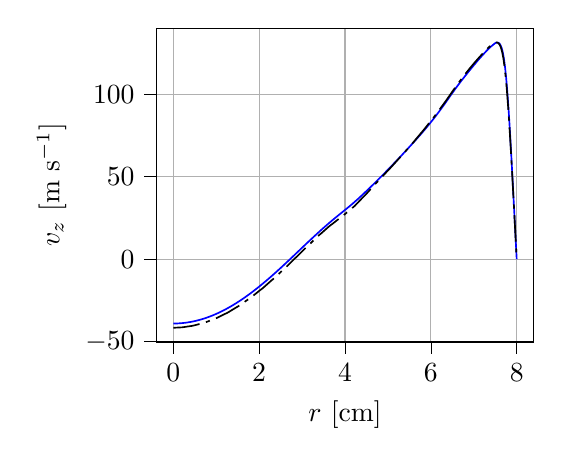
\begin{tikzpicture}

\definecolor{darkgray176}{RGB}{176,176,176}

\begin{axis}[
legend cell align=left,
legend pos= north east,
scale = .7,
ylabel = {$v_z$ [m s$^{-1}$]},
tick align=outside,
tick pos=left,
xlabel = {$r$ [cm]},
x grid style={darkgray176},
xmajorgrids,
xmin=-0.399999991059303, xmax=8.39999981224537,
xtick style={color=black},
y grid style={darkgray176},
ymajorgrids,
ymin=-50.2193093021143, ymax=139.927959246206,
ytick style={color=black}
]
\addplot [semithick, blue]
table {%
0 -39.0015382752699
0.007999999797903 -38.9967398141904
0.015999999595806 -38.9919413545988
0.023999999393709 -38.987142896495
0.031999999191612 -38.9823444398792
0.039999998989515 -38.9775459847515
0.047999998787418 -38.9727475311117
0.0560000014957041 -38.9679490772143
0.063999998383224 -38.9631506282963
0.0720000010915101 -38.9583521773753
0.07999999797903 -38.9535537314338
0.0880000006873161 -38.9487552834893
0.095999997574836 -38.9439568405244
0.104000000283122 -38.9360010576152
0.112000002991408 -38.921605744084
0.119999994058162 -38.9072104560694
0.127999996766448 -38.8928151516759
0.135999999474734 -38.8784198518513
0.14400000218302 -38.8640245565961
0.151999993249774 -38.8496292868582
0.15999999595806 -38.8352340007418
0.167999998666346 -38.8208387191952
0.176000001374632 -38.8064434422184
0.183999992441386 -38.7920481907594
0.191999995149672 -38.7776529229227
0.199999986216426 -38.7632576806041
0.208000000566244 -38.7425669447433
0.215999991632998 -38.7186040917334
0.224000005982816 -38.6946411766083
0.23199999704957 -38.6706783388505
0.239999988116324 -38.6467155087193
0.248000002466142 -38.6227526164737
0.255999993532896 -38.5987898015961
0.26399998459965 -38.5748269943459
0.271999998949468 -38.5508641249822
0.279999990016222 -38.5269013329871
0.28800000436604 -38.502938478879
0.295999995432794 -38.4789757021402
0.303999986499548 -38.4550129330297
0.312000000849366 -38.4216486211081
0.31999999191612 -38.3881605044745
0.327999982982874 -38.3546723985148
0.335999997332692 -38.3211842057656
0.343999988399446 -38.2876961211542
0.352000002749264 -38.2542079497542
0.359999993816018 -38.2207198864925
0.367999984882772 -38.1872318339062
0.37599999923259 -38.1537436945324
0.383999990299344 -38.120255663298
0.392000004649162 -38.0867675452768
0.399999972432852 -38.0532796328585
0.40799998678267 -38.0167990754992
0.416000001132488 -37.973840856999
0.423999968916178 -37.9308829022866
0.431999983265996 -37.8879247112637
0.439999997615814 -37.8449665339801
0.448000011965632 -37.8020083704362
0.455999979749322 -37.7590504706813
0.46399999409914 -37.7160923346182
0.472000008448958 -37.6731342122961
0.479999976232648 -37.6301763537643
0.487999990582466 -37.5872182589257
0.496000004932284 -37.5442601778296
0.503999972715974 -37.5013023605245
0.511999987065792 -37.4522802563209
0.52000000141561 -37.3999204306657
0.5279999691993 -37.3475609265771
0.535999983549118 -37.2952011345085
0.543999997898936 -37.242841359234
0.551999965682626 -37.1904819055277
0.559999980032444 -37.1381221638433
0.567999994382262 -37.0857624389547
0.57600000873208 -37.0334027308625
0.58399997651577 -36.9810433443402
0.591999990865588 -36.9286836698423
0.600000005215406 -36.8763240121424
0.607999972999096 -36.8239646760138
0.615999987348914 -36.7625270133926
0.624000001698732 -36.700846928928
0.631999969482422 -36.6391672233813
0.63999998383224 -36.5774871787037
0.647999998182058 -36.5158071539204
0.655999965965748 -36.4541275080567
0.663999980315566 -36.3924475230642
0.671999994665384 -36.3307675579683
0.679999962449074 -36.2690879717932
0.687999976798892 -36.2074080464918
0.69599999114871 -36.1457281410887
0.704000005498528 -36.0840482555847
0.711999973282218 -36.0195733419878
0.719999987632036 -35.9486673702218
0.728000001981854 -35.8777614214926
0.735999969765544 -35.8068559085269
0.743999984115362 -35.7359500058733
0.75199999846518 -35.6650441262587
0.75999996624887 -35.5941386824094
0.767999980598688 -35.523232848875
0.775999994948506 -35.4523270383817
0.784000009298325 -35.3814212509305
0.791999977082014 -35.310515899247
0.799999944865704 -35.2396105706067
0.808000005781651 -35.1687044395608
0.81599997356534 -35.0920362064885
0.82399994134903 -35.0120122452853
0.832000002264977 -34.9319873787164
0.839999970048666 -34.8519634699929
0.847999937832355 -34.7719395875101
0.855999998748302 -34.6919147996653
0.863999966531992 -34.6118909696672
0.871999934315681 -34.5318671659127
0.879999995231628 -34.4518424567995
0.887999963015318 -34.3718187055347
0.896000023931265 -34.2917940489136
0.903999991714954 -34.211770350142
0.911999959498644 -34.1317466776181
0.920000020414591 -34.0430747112339
0.92799998819828 -33.9540527930253
0.93599995598197 -33.8650309043589
0.944000016897917 -33.7760080088811
0.951999984681606 -33.6869861793029
0.959999952465296 -33.5979643792698
0.968000013381243 -33.5089415724291
0.975999981164932 -33.4199198314898
0.983999948948622 -33.3308981200987
0.992000009864569 -33.2418754019037
0.999999977648258 -33.152853749612
1.00799994543195 -33.0638321268712
1.01600000634789 -32.9724482729972
1.02399997413158 -32.8744922267161
1.03199994191527 -32.7765363233099
1.04000000283122 -32.6785794223934
1.04799997061491 -32.5806238046599
1.0559999383986 -32.4826683297225
1.06399999931455 -32.3847118572016
1.07199996709824 -32.28675666778
1.07999993488193 -32.1888016210755
1.08799999579787 -32.0908455767149
1.09599996358156 -31.9928908153695
1.10399993136525 -31.8949361966632
1.1119999922812 -31.7969805802262
1.11999996006489 -31.6967881837506
1.12800002098083 -31.5899846367428
1.13599998876452 -31.4831824914432
1.14399995654821 -31.3763805044746
1.15200001746416 -31.2695774324668
1.15999998524785 -31.1627757620742
1.16799995303154 -31.0559742499267
1.17600001394749 -30.949171652658
1.18399998173118 -30.8423704569114
1.19199994951487 -30.7355694193242
1.20000001043081 -30.6287672965338
1.2079999782145 -30.5219665751738
1.21599994599819 -30.4151660118841
1.22400000691414 -30.3064951271993
1.23199997469783 -30.1910374744085
1.23999994248152 -30.0755799952045
1.24800000339746 -29.9601213454512
1.25599997118115 -29.8446642133273
1.26399993896484 -29.7292072546937
1.27199999988079 -29.6137491254237
1.27999996766448 -29.4982925136806
1.28799993544817 -29.3828360753319
1.29599999636412 -29.2673784662592
1.30399996414781 -29.1519223746113
1.3119999319315 -29.0364664562642
1.31999999284744 -28.9210093671
1.32799996063113 -28.8040452431744
1.33599992841482 -28.6801567767104
1.34399998933077 -28.5562670565265
1.35199995711446 -28.4323789670983
1.35999992489815 -28.3084910661353
1.36799998581409 -28.1846019113537
1.37599995359778 -28.0607143872212
1.38400001451373 -27.9368256092054
1.39199998229742 -27.8129384617602
1.39999995008111 -27.6890515026124
1.40800001099706 -27.5651632894839
1.41599997878075 -27.441276706818
1.42399994656444 -27.3173903123414
1.43200000748038 -27.1923427320291
1.43999997526407 -27.060281628857
1.44799994304776 -26.9282207288641
1.45600000396371 -26.7961584946196
1.4639999717474 -26.6640980008764
1.47199993953109 -26.5320377101988
1.48000000044703 -26.3999760851695
1.48799996823072 -26.2679162005206
1.49599993601441 -26.1358565188258
1.50399999693036 -26.0037955026767
1.51199996471405 -25.8717362267886
1.51999993249774 -25.7396771537458
1.52799999341369 -25.6076167461386
1.53599996119738 -25.4747311782713
1.54399992898107 -25.3347892057337
1.55199998989701 -25.1948458215579
1.5599999576807 -25.05490428399
1.56800001859665 -24.9149613347094
1.57599989324808 -24.7750218610835
1.58399995416403 -24.6350793465392
1.59200001507998 -24.4951370493018
1.59999988973141 -24.3551982275849
1.60799995064735 -24.215256364847
1.6160000115633 -24.0753147192962
1.62399988621473 -23.9353765491345
1.63199994713068 -23.795435337841
1.64000000804663 -23.6549809703501
1.64799988269806 -23.507485274985
1.65599994361401 -23.3599863769012
1.66400000452995 -23.2124877102648
1.67199987918139 -23.0649927092203
1.67999994009733 -22.917494505343
1.68800000101328 -22.769996532793
1.69599987566471 -22.6225022256887
1.70399993658066 -22.4750047156412
1.7119999974966 -22.3275074367954
1.71999987214804 -22.1800138232516
1.72799993306398 -22.0325170066577
1.73599999397993 -21.8850204211312
1.74399986863136 -21.7373047039076
1.75199992954731 -21.5826091081701
1.75999999046326 -21.427913757484
1.7680000513792 -21.2732186518046
1.77599992603064 -21.1185273928273
1.78399998694658 -20.9638327770172
1.79200004786253 -20.8091384060877
1.79999992251396 -20.6544478817052
1.80799998342991 -20.4997540003736
1.81600004434586 -20.3450603637889
1.82399991899729 -20.1903705735996
1.83199997991323 -20.0356774263482
1.84000004082918 -19.8809845237016
1.84799991548061 -19.7262954673041
1.85599997639656 -19.564836826512
1.86400003731251 -19.4033376705936
1.87199991196394 -19.2418425331215
1.87999997287989 -19.0803438937274
1.88800003379583 -18.9188455125232
1.89599990844727 -18.7573511496154
1.90399996936321 -18.5958532846582
1.91200003027916 -18.4343556777503
1.91999990493059 -18.2728620889791
1.92799996584654 -18.111364998035
1.93600002676249 -17.9498681650034
1.94399990141392 -17.7883753499408
1.95199996232986 -17.626879032587
1.96000002324581 -17.459275917838
1.96799989789724 -17.2914031763435
1.97599995881319 -17.1235267973053
1.98400001972914 -16.9556506893304
1.99199989438057 -16.7877787609943
1.99999995529652 -16.6199031949962
2.00800001621246 -16.4520278999085
2.0159998908639 -16.2841567842939
2.02399995177984 -16.1162820308866
2.03200001269579 -15.9484075482415
2.03999988734722 -15.7805372449073
2.04799994826317 -15.6126633036423
2.05600000917912 -15.4447896329966
2.06399988383055 -15.2718279260731
2.07199994474649 -15.0977472791392
2.08000000566244 -14.9236659512326
2.08799988031387 -14.7495879960753
2.09599994122982 -14.5755053079856
2.10400000214577 -14.4014219406684
2.1119998767972 -14.227341947891
2.11999993771315 -14.0532572238754
2.12799999862909 -13.8791718223714
2.13599987328053 -13.7050897971919
2.14399993419647 -13.531003042462
2.15199999511242 -13.3569156119772
2.15999986976385 -13.1828315595954
2.1679999306798 -13.0071620377988
2.17599999159575 -12.8276077090545
2.18399986624718 -12.6480568476752
2.19199992716312 -12.468501093149
2.19999998807907 -12.2889446266342
2.2079998627305 -12.1093916293551
2.21599992364645 -11.9298337406914
2.2239999845624 -11.7502751418643
2.23199985921383 -11.5707200141418
2.23999992012978 -11.391159996799
2.24799998104572 -11.2115992710953
2.25600004196167 -11.0320378376331
2.2639999166131 -10.852479877747
2.27199997752905 -10.6729170305879
2.280000038445 -10.4900956647833
2.28799991309643 -10.3055865281791
2.29599997401237 -10.1210723597143
2.30400003492832 -9.9365574560101
2.31199990957975 -9.7520461137557
2.3199999704957 -9.56752974146064
2.32800003141165 -9.38301263579495
2.33599990606308 -9.19849909349925
2.34399996697903 -9.01398052297596
2.35200002789497 -8.82946122094593
2.35999990254641 -8.64494548419622
2.36799996346235 -8.46042472102768
2.3760000243783 -8.27590322820891
2.38399989902973 -8.09126752791444
2.39199995994568 -7.90240534801207
2.40000002086163 -7.713542416743
2.40799989551306 -7.52468313204325
2.415999956429 -7.33581869996385
2.42400001734495 -7.14695351842162
2.43199989199638 -6.95809198540264
2.43999995291233 -6.76922530684941
2.44800001382828 -6.58035788073435
2.45599988847971 -6.39149410508824
2.46399994939566 -6.20262518575059
2.4720000103116 -6.01375552073858
2.47999988496304 -5.82488950813827
2.48799994587898 -5.63601835368103
2.49600000679493 -5.4457070982422
2.50399988144636 -5.25320381113352
2.51199994236231 -5.06069528277816
2.52000000327826 -4.86818599594326
2.52799987792969 -4.67568043346594
2.53599993884563 -4.48316963160477
2.54399999976158 -4.29065807317024
2.55199987441301 -4.0981502410584
2.55999993532896 -3.90563717144119
2.56799999624491 -3.71312334715083
2.57599987089634 -3.52061325114057
2.58399993181229 -3.32809791945343
2.59199999272823 -3.135581835009
2.59999986737967 -2.94306948079585
2.60799992829561 -2.74838265313582
2.61599998921156 -2.55302743965147
2.62399986386299 -2.35767601371519
2.63199992477894 -2.1623192790631
2.63999998569489 -1.96696178477509
2.64799986034632 -1.77160808000106
2.65599992126226 -1.57624906836876
2.66399998217821 -1.38088929900947
2.67199985682964 -1.18553332112334
2.67999991774559 -0.990172038230533
2.68799997866154 -0.794809999512677
2.69599985331297 -0.599451754221105
2.70399991422892 -0.404088205767972
2.71199997514486 -0.208464710768963
2.7199998497963 -0.0111597549934251
2.72799991071224 0.186150552680953
2.73599997162819 0.383461617693447
2.74399984627962 0.580768845413491
2.75199990719557 0.778081423186756
2.75999996811152 0.975394756426144
2.76800002902746 1.17270884443245
2.77599990367889 1.37001909256557
2.78399996459484 1.56733468830573
2.79200002551079 1.76465103696871
2.79999990016222 1.96196354380596
2.80799996107817 2.1592813964136
2.81600002199411 2.35660000006237
2.82399989664555 2.55439549053321
2.83199995756149 2.7526735715538
2.84000001847744 2.95095240270291
2.84799989312887 3.14922736682598
2.85599995404482 3.3475076963415
2.86400001496077 3.54578877411372
2.8719998896122 3.7440659829438
2.87999995052814 3.94234855536664
2.88800001144409 4.14063187413261
2.89599988609552 4.33891132206218
2.90399994701147 4.5371961317597
2.91200000792742 4.73548168598934
2.91999988257885 4.93376336744648
2.9279999434948 5.13205040886848
2.93600000441074 5.33023143862582
2.94399987906218 5.52839268128567
2.95199993997812 5.72655927635851
2.96000000089407 5.92472660936706
2.9679998755455 6.1228900657661
2.97599993646145 6.321058872794
2.9839999973774 6.51922841592427
2.99199987202883 6.71739408056167
2.99999993294477 6.91556509404998
3.00799999386072 7.113736841813
3.01599986851215 7.31190470920668
3.0239999294281 7.51007792367895
3.03199999034405 7.70825187060439
3.03999986499548 7.90611234574626
3.04799992591143 8.10299037028577
3.05599998682737 8.29986911971402
3.06399986147881 8.49674400950084
3.07199992239475 8.69362420689301
3.0799999833107 8.89050512737873
3.08799985796213 9.08738218640021
3.09599991887808 9.28426455125583
3.10399997979403 9.48114763741414
3.11199985444546 9.67802686026102
3.1199999153614 9.87491138723757
3.12799997627735 10.0717966337351
3.1360000371933 10.2686825991604
3.14400009810925 10.4655692829209
3.15199978649616 10.6682134008897
3.15999984741211 10.861656862704
3.16799990832806 11.0551002048099
3.175999969244 11.2485434275838
3.18400003015995 11.4419865314007
3.1920000910759 11.6354295166339
3.19999977946281 11.828863375841
3.20799984037876 12.0223061250259
3.21599990129471 12.2157487567377
3.22399996221066 12.4091912713435
3.2320000231266 12.602633669209
3.24000008404255 12.7960759506982
3.24799977242947 12.9895091083921
3.25599983334541 13.1829511582202
3.26399989426136 13.3759285545899
3.27199995517731 13.5678152147305
3.28000001609325 13.7597017591015
3.2880000770092 13.9515881880618
3.29599976539612 14.1434655666366
3.30399982631207 14.3353517658512
3.31199988722801 14.5272378507226
3.31999994814396 14.7191238216346
3.32800000905991 14.9110096788462
3.33600006997585 15.1028954227999
3.34399975836277 15.2947721185131
3.35199981927872 15.4866576369388
3.35999988019466 15.6785430431173
3.36799994111061 15.8704283373929
3.37600000202656 16.0623135201086
3.3840000629425 16.2500427050901
3.39199975132942 16.4377232058425
3.39999981224537 16.6254123369176
3.40799987316132 16.8131013587527
3.41599993407726 17.0007902716808
3.42399999499321 17.1884790760338
3.43200005590916 17.3761677721783
3.43999974429607 17.5638476204721
3.44799980521202 17.7515361010811
3.45599986612797 17.9392244744284
3.46399992704391 18.1269127408389
3.47199998795986 18.3146009006365
3.48000004887581 18.5022889541434
3.48799973726273 18.6899681618489
3.49599979817867 18.8737981977307
3.50399985909462 19.0558312960128
3.51199992001057 19.2378642918717
3.51999998092651 19.4198971856157
3.52800004184246 19.6019299775515
3.53600010275841 19.7839626679852
3.54399979114532 19.9659867807349
3.55199985206127 20.148019269081
3.55999991297722 20.3300516568348
3.56799997389317 20.512083944297
3.57600003480911 20.6941161317675
3.58400009572506 20.8761482195446
3.59199978411198 21.0581717314676
3.59999984502792 21.2402036207536
3.60799990594387 21.4200169133368
3.61599996685982 21.5961167232493
3.62400002777576 21.7722164382778
3.63200008869171 21.948316058704
3.63999977707863 22.1244073845997
3.64799983799458 22.3005068166659
3.65599989891052 22.4766061549677
3.66399995982647 22.6527053997824
3.67200002074242 22.828804551386
3.68000008165836 23.0049036100534
3.68799977004528 23.1809943758762
3.69599983096123 23.3570932494963
3.70399989187717 23.5331920309987
3.71199995279312 23.7092907206541
3.72000001370907 23.8850588342595
3.72800007462502 24.0561298287481
3.73599976301193 24.2271927698053
3.74399982392788 24.3982635897852
3.75199988484383 24.5693343228913
3.75999994575977 24.7404049693775
3.76800000667572 24.9114755294965
3.77600006759167 25.0825460035084
3.78399975597858 25.2536084256161
3.79199981689453 25.4246787281445
3.79999987781048 25.5957489453072
3.80799993872643 25.7668190773519
3.81599999964237 25.9378891245258
3.82400006055832 26.1089590870748
3.83199974894524 26.2800209992446
3.83999980986118 26.4488628691604
3.84799987077713 26.6169910803182
3.85599993169308 26.7851192110443
3.86399999260902 26.9532472615706
3.87200005352497 27.1213752321283
3.87999974191189 27.2894952939441
3.88799980282784 27.4576231052582
3.89599986374378 27.6257508372918
3.90399992465973 27.7938784902724
3.91199998557568 27.9620060644268
3.92000004649162 28.130133559981
3.92799973487854 28.2982531481783
3.93599979579449 28.4663804872097
3.94399985671043 28.6345077483131
3.95199991762638 28.8027813937818
3.95999997854233 28.9712346140207
3.96800003945827 29.139687759444
3.97599972784519 29.3081329861188
3.98399978876114 29.4765859825526
3.99199984967709 29.6450389048073
3.99999991059303 29.8134917530935
4.00799997150898 29.9819445276208
4.01600003242493 30.1503972285983
4.02400009334087 30.3188498562342
4.03199978172779 30.4872945666138
4.03999984264374 30.6557470481911
4.04799990355968 30.8241994570465
4.05599996447563 30.9926517933851
4.06400002539158 31.1617764408096
4.07200008630753 31.335003929592
4.07999977469444 31.5082232810436
4.08799983561039 31.6814506283011
4.09599989652634 31.8546779050923
4.10399995744228 32.0279051116147
4.11200001835823 32.2011322480653
4.12000007927418 32.3743593146402
4.12799976766109 32.5475782450868
4.13599982857704 32.7208051724987
4.14399988949299 32.8940320306186
4.15199995040894 33.0672588196399
4.16000001132488 33.2404855397551
4.16800007224083 33.4137121911559
4.17599976062775 33.586930707605
4.18399982154369 33.7688195662974
4.19199988245964 33.952452099613
4.19999994337559 34.1360845643339
4.20800000429153 34.3197169606503
4.21600006520748 34.5033492887515
4.2239997535944 34.6869729978494
4.23199981451035 34.8706051900884
4.23999987542629 35.0542373146761
4.24799993634224 35.2378693717987
4.25599999725819 35.4215013616424
4.26400005817413 35.6051332843921
4.27199974656105 35.7887565892746
4.279999807477 35.9723883783925
4.28799986839294 36.1560201009681
4.29599992930889 36.332242871653
4.30399999022484 36.5246820258583
4.31200005114079 36.7171215876559
4.3199997395277 36.9095525970444
4.32799980044365 37.1019929773846
4.3359998613596 37.2944337687023
4.34399992227554 37.4868749721344
4.35199998319149 37.6793165888217
4.36000004410744 37.8717586199094
4.36799973249435 38.0641921053058
4.3759997934103 38.2566349686275
4.38399985432625 38.4490782498105
4.3919999152422 38.6415219500171
4.39999997615814 38.8339660704139
4.40800003707409 39.0280807467494
4.41599972546101 39.2252371750301
4.42399978637695 39.4224031300941
4.4319998472929 39.6195694317461
4.43999990820885 39.8167360809555
4.44799996912479 40.0139030786952
4.45600003004074 40.2110704259419
4.46399971842766 40.4082289424013
4.47199977934361 40.6053969915901
4.47999984025955 40.8025653932379
4.4879999011755 40.9997341483358
4.49599996209145 41.1969032578791
4.50400002300739 41.3940727228664
4.51200008392334 41.5912425443005
4.51999977231026 41.7891607739124
4.5279998332262 41.9904570569689
4.53599989414215 42.1917536431609
4.5439999550581 42.3930505333468
4.55200001597404 42.5943477283881
4.56000007688999 42.7956452291496
4.56799976527691 42.9969336629039
4.57599982619286 43.1982317776955
4.5839998871088 43.3995302008278
4.59199994802475 43.6008289331689
4.6000000089407 43.8021279756035
4.60800006985664 44.003427329016
4.61599975824356 44.2047176206127
4.62399981915951 44.4060175986343
4.63199988007545 44.6073178903082
4.6399999409914 44.812326628621
4.64800000190735 45.0172865188009
4.6560000628233 45.2222466861369
4.66399975121021 45.4271975872768
4.67199981212616 45.6321583113033
4.67999987304211 45.8371193148831
4.68799993395805 46.0420805988193
4.695999994874 46.2470421639264
4.70400005578995 46.4520040110097
4.71199974417686 46.6569565966587
4.71999980509281 46.8619190101318
4.72799986600876 47.066881708036
4.73599992692471 47.2718446911953
4.74399998784065 47.4768079604369
4.7520000487566 47.684571922389
4.75999973714352 47.8928463663674
4.76799979805946 48.1011307710252
4.77599985897541 48.309415438218
4.78399991989136 48.5177003687111
4.7919999808073 48.7259855632722
4.80000004172325 48.9342710226724
4.80799973011017 49.1425470486934
4.81599979102612 49.3508330400842
4.82399985194206 49.559119298645
4.83199991285801 49.7674058251588
4.83999997377396 49.975692620412
4.8480000346899 50.1839796851935
4.85599972307682 50.3922573212285
4.86399978399277 50.6026391045912
4.87199984490871 50.8140365538599
4.87999990582466 51.0254342560782
4.88799996674061 51.2368322119926
4.89600002765656 51.4482304223525
4.90399971604347 51.6596190439711
4.91199977695942 51.8710177654702
4.91999983787537 52.0824167436808
4.92799989879131 52.2938159793643
4.93599995970726 52.5052154732851
4.94400002062321 52.7166152262106
4.95199970901012 52.9280053948998
4.95999976992607 53.1394056681367
4.96799983084202 53.3508062026987
4.97599989175797 53.5637314037996
4.98399995267391 53.7781591213857
4.99200001358986 53.9925870842086
4.99999970197678 54.2070053079808
5.00799976289272 54.4214337634701
5.01599982380867 54.6358624664067
5.02399988472462 54.850291417533
5.03199994564056 55.0647206175948
5.04000000655651 55.2791500673407
5.04800006747246 55.4935797675225
5.05599975585938 55.7079997337923
5.06399981677532 55.9224299371011
5.07199987769127 56.1368603931189
5.07999993860722 56.3512911026095
5.08799999952316 56.5667478375094
5.09600006043911 56.7842505053776
5.10399974882603 57.0017432773723
5.11199980974197 57.2192464105802
5.11999987065792 57.4367497775238
5.12799993157387 57.654253378914
5.13599999248981 57.8717572154643
5.14400005340576 58.0892612878914
5.15199974179268 58.3067554686528
5.15999980270863 58.5242600149837
5.16799986362457 58.7417647993588
5.17599992454052 58.9592698225062
5.18399998545647 59.1767750851573
5.19200004637241 59.3942805880463
5.19999973475933 59.612309325276
5.20799979567528 59.8330591151474
5.21599985659122 60.0538091121965
5.22399991750717 60.2745593170609
5.23199997842312 60.4953097303813
5.24000003933907 60.7160603528006
5.24799972772598 60.9368009055263
5.25599978864193 61.157551948069
5.26399984955788 61.3783032016645
5.27199991047382 61.5990546669533
5.27999997138977 61.8198063445963
5.28800003230572 62.0405582352525
5.29599972069263 62.2613000600864
5.30399978160858 62.4820523787478
5.31199984252453 62.7028049124163
5.31999990344048 62.927083177105
5.32799996435642 63.1513796753109
5.33600002527237 63.3756763358632
5.34399971365929 63.5999627147105
5.35199977457523 63.8242597014729
5.35999983549118 64.048556852111
5.36799989640713 64.2728541671326
5.37599995732307 64.497151647072
5.38400001823902 64.7214492924295
5.39199970662594 64.9457366591264
5.39999976754189 65.1700346368879
5.40799982845783 65.3943327816415
5.41599988937378 65.6186310939143
5.42399995028973 65.8429295742355
5.43200001120567 66.0644191359716
5.43999969959259 66.2921794700826
5.44799976050854 66.5199503855761
5.45599982142448 66.7477212760993
5.46399988234043 66.9754921416301
5.47199994325638 67.2032629821465
5.48000000417233 67.4310337976223
5.48799969255924 67.6587939817248
5.49599975347519 67.8865647470663
5.50399981439114 68.1143354873049
5.51199987530708 68.3421062024183
5.51999993622303 68.5698768923842
5.52799999713898 68.7976475571805
5.53600005805492 69.0261894698268
5.54399974644184 69.2552995109476
5.55199980735779 69.4844201998974
5.55999986827374 69.7135408674738
5.56799992918968 69.9426615136577
5.57599999010563 70.1717821384302
5.58400005102158 70.400902741772
5.59199973940849 70.6300126544882
5.59999980032444 70.8591332149135
5.60799986124039 71.0882537538512
5.61599992215633 71.3173742712824
5.62399998307228 71.546494767188
5.63200004398823 71.7756152415487
5.63999973237514 72.0061794617929
5.64799979329109 72.2398890181464
5.65599985420704 72.473598555378
5.66399991512299 72.7073080734709
5.67199997603893 72.9410175724078
5.68000003695488 73.1747270521719
5.6879997253418 73.4084256298747
5.69599978625774 73.6421350712039
5.70399984717369 73.8758444933962
5.71199990808964 74.1095538962987
5.71999996900558 74.3432632799427
5.72800002992153 74.5769726443111
5.73599971830845 74.8106711065306
5.7439997792244 75.0448291746185
5.75199984014034 75.2857022223266
5.75999990105629 75.526575252019
5.76799996197224 75.7674482636794
5.77600002288818 76.0083212572919
5.7839997112751 76.2491830164041
5.79199977219105 76.4900559738396
5.79999983310699 76.7309289132257
5.80799989402294 76.9718018345055
5.81599995493889 77.2126747376367
5.82400001585484 77.4535476226228
5.83199970424175 77.6944092730166
5.8399997651577 77.9352821216648
5.84799982607365 78.1761549521193
5.85599988698959 78.4243627099248
5.86399994790554 78.6743093936643
5.87200000882149 78.9242560595977
5.8799996972084 79.17419106875
5.88799975812435 79.4241376990236
5.8959998190403 79.6740843114431
5.90399987995625 79.9240309059886
5.91199994087219 80.1739774826551
5.92000000178814 80.4239240414156
5.92799969017506 80.6738589433039
5.935999751091 80.9238054662123
5.94399981200695 81.17375197117
5.9519998729229 81.423698458161
5.95999993383884 81.679362781394
5.96799999475479 81.9396287335181
5.97599968314171 82.1998825479506
5.98399974405766 82.4601484636448
5.9919998049736 82.720414361099
5.99999986588955 82.9806802402967
6.0079999268055 83.2409461012211
6.01599998772144 83.5012119438573
6.02400004863739 83.7614777681871
6.03199973702431 84.0217314547163
6.03999979794025 84.2819972423858
6.0479998588562 84.5422630117
6.05599991977215 84.8025287626422
6.0639999806881 85.0660626855984
6.07200004160404 85.3372291442777
6.07999972999096 85.608382956908
6.08799979090691 85.8795493776224
6.09599985182285 86.1507157793282
6.1039999127388 86.4218821620081
6.11199997365475 86.6930485256325
6.12000003457069 86.9642148701687
6.12799972295761 87.2353685686513
6.13599978387356 87.5065348750565
6.14399984478951 87.7777011623497
6.15199990570545 88.0488674305134
6.1599999666214 88.3200336795304
6.16800002753735 88.5916926773413
6.17599971592426 88.8736631908655
6.18399977684021 89.1556468153432
6.19199983775616 89.4376304199692
6.1999998986721 89.7196140047255
6.20799995958805 90.001597569594
6.216000020504 90.2835811145156
6.22399970889091 90.5655515087936
6.23199976980686 90.8475350139125
6.23999983072281 91.1295184990501
6.24799989163876 91.4115019642095
6.2559999525547 91.6934854093724
6.26399964094162 91.9754557037446
6.2720000743866 92.2574522396361
6.27999976277351 92.5473902263197
6.28800019621849 92.8394569639483
6.29599988460541 93.1314964816924
6.30399957299232 93.423535978895
6.3120000064373 93.7156026548918
6.31999969482422 94.0076421109536
6.3280001282692 94.2997087457647
6.33599981665611 94.591748160614
6.34399950504303 94.8837875548246
6.35199993848801 95.1758541277258
6.35999962687492 95.4678934806075
6.3680000603199 95.7599600121382
6.37599974870682 96.0519993236155
6.38400018215179 96.3487153864421
6.39199987053871 96.6494118114936
6.39999955892563 96.9501082158282
6.40799999237061 97.2508326050499
6.41599968075752 97.551528967892
6.4240001142025 97.8522533155792
6.43199980258942 98.1529496368516
6.43999949097633 98.4536459373142
6.44799992442131 98.7543702225581
6.45599961280823 99.0550664813367
6.4640000462532 99.3557907248556
6.47199973464012 99.6564869418749
6.4800001680851 99.9572111435923
6.48799985647202 100.207922797956
6.49599954485893 100.500005199769
6.50399997830391 100.792114573873
6.51199966669083 101.084196513553
6.5200001001358 101.376305425438
6.52799978852272 101.668386902889
6.5360002219677 101.960495352405
6.54399991035461 102.252576367462
6.55199959874153 102.544657151283
6.56000003218651 102.836764907003
6.56799972057343 103.128845228256
6.5760001540184 103.420952521286
6.58399984240532 103.7130323798
6.59199953079224 103.995862858277
6.59999996423721 104.272664554979
6.60799965262413 104.549440288542
6.61600008606911 104.826241614432
6.62399977445602 105.103016977184
6.632000207901 105.379817932184
6.63999989628792 105.656592924003
6.64799958467484 105.933367730323
6.65600001811981 106.210168128758
6.66399970650673 106.486942563982
6.67200013995171 106.763742591263
6.67999982833862 107.0405166553
6.68799951672554 107.317290533706
6.69599995017052 107.584756559652
6.70399963855743 107.851451812581
6.71200007200241 108.118171756257
6.71999976038933 108.384866712938
6.7280001938343 108.651586360311
6.73599988222122 108.918281020642
6.74399957060814 109.184975532773
6.75200000405312 109.451694735489
6.75999969244003 109.71838895114
6.76800012588501 109.985107857306
6.77599981427193 110.251801776425
6.78399950265884 110.518495547217
6.79199993610382 110.783504628131
6.79999962449074 111.043298080594
6.80800005793571 111.303115608521
6.81599974632263 111.562908819717
6.82400017976761 111.822726106343
6.83199986815453 112.082519076235
6.83999955654144 112.342311925443
6.84799998998642 112.602128849967
6.85599967837334 112.861921457739
6.86400011181831 113.121738140771
6.87199980020523 113.381530507061
6.87999948859215 113.641322752568
6.88799992203712 113.901139073251
6.89599961042404 114.157646306386
6.90400004386902 114.411693009217
6.91199973225594 114.665715949117
6.92000016570091 114.919762443362
6.92799985408783 115.173785174683
6.93599954247475 115.427807801691
6.94399997591972 115.681853982976
6.95199966430664 115.9358764013
6.96000009775162 116.189922373853
6.96799978613853 116.443944583432
6.97599947452545 116.697966688649
6.98399990797043 116.952012348007
6.99199959635735 117.206034244378
7.00000002980232 117.454122529161
7.00799971818924 117.701459587056
7.01600015163422 117.948819580406
7.02399984002113 118.196156437346
7.03199952840805 118.443493193784
7.03999996185303 118.69085288562
7.04799965023994 118.938189441001
7.05600008368492 119.185548931731
7.06399977207184 119.432885285996
7.07200020551682 119.680244575561
7.07999989390373 119.927580728682
7.08799958229065 120.174916781182
7.09600001573563 120.420222043927
7.10399970412254 120.657910383013
7.11200013756752 120.895620748823
7.11999982595444 121.133308866721
7.12799951434135 121.370996874034
7.13599994778633 121.608706907989
7.14399963617325 121.846394694025
7.15200006961823 122.084104506651
7.15999975800514 122.321792071345
7.16800019145012 122.559501662576
7.17599987983704 122.797189005886
7.18399956822395 123.034876238464
7.19200000166893 123.272585497502
7.19999969005585 123.502436614935
7.20800012350082 123.725486785507
7.21599981188774 123.948516047974
7.22399950027466 124.171545174354
7.23199993371964 124.39459493665
7.23999962210655 124.617623790818
7.24800005555153 124.840673280817
7.25599974393845 125.063701862674
7.26400017738342 125.286751080296
7.27199986577034 125.509779389762
7.27999955415726 125.732807563032
7.28799998760223 125.955856371959
7.29599967598915 126.17888427271
7.30400010943413 126.383335602268
7.31199979782104 126.584648598902
7.31999948620796 126.785961417247
7.32799991965294 126.987292806737
7.33599960803986 127.188605268458
7.34400004148483 127.389936301213
7.35199972987175 127.591248406182
7.36000016331673 127.792579082099
7.36799985170364 127.99389083021
7.37599954009056 128.195202399862
7.38399997353554 128.396532540359
7.39199966192245 128.597843753008
7.40000009536743 128.793681495879
7.40799978375435 128.964173474091
7.41599947214127 129.134665213668
7.42399990558624 129.305172593429
7.43199959397316 129.475663855611
7.44000002741814 129.646170757872
7.44799971580505 129.81666154251
7.45600014925003 129.987167967113
7.46399983763695 130.157658274068
7.47199952602386 130.328148342141
7.47999995946884 130.49865405002
7.48799964785576 130.669143640207
7.49600008130074 130.839648870074
7.50399976968765 130.961195215655
7.51200020313263 131.048525251919
7.51999989151955 131.122539395121
7.52799957990646 131.177922846675
7.53600001335144 131.219940036964
7.54399970173836 131.235211043656
7.55200013518333 131.237649277769
7.55999982357025 131.201588974254
7.56799951195717 131.154599733722
7.57599994540215 131.052934720569
7.58399963378906 130.944374003172
7.59200006723404 130.75979730603
7.59999975562096 130.575237798002
7.60800018906593 130.287396799622
7.61599987745285 129.999579452987
7.62399956583977 129.595662375761
7.63199999928474 129.181149552417
7.63999968767166 128.639092828649
7.64800012111664 128.07146561015
7.65599980950356 127.36694842989
7.66399949789047 126.616784956962
7.67199993133545 125.727505714076
7.67999961972237 124.768198317855
7.68800005316734 123.671386370112
7.69599974155426 122.476522077791
7.70400017499924 121.151299665148
7.71199986338615 119.695963243931
7.71999955177307 118.124876175968
7.72799998521805 116.391549966673
7.73599967360497 114.562519048032
7.74400010704994 112.541544020812
7.75199979543686 110.448296952325
7.75999948382378 108.137650779241
7.76799991726875 105.779367659904
7.77599960565567 103.184183750232
7.78400003910065 100.566118147164
7.79199972748756 97.6992822470413
7.80000016093254 94.832179341618
7.80799984931946 91.7141269301335
7.81599953770638 88.596079572357
7.82399997115135 85.2731238182706
7.83199965953827 81.9318645456619
7.84000009298325 78.4294643877319
7.84799978137016 74.8958686673662
7.85599946975708 71.2400774941558
7.86399990320206 67.5432021707051
7.87199959158897 63.7628712787724
7.88000002503395 59.9402796670149
7.88799971342087 56.0640563156017
7.89600014686584 52.148903682303
7.90399983525276 48.2023694542081
7.91199952363968 44.2240888821441
7.91999995708466 40.2293881158346
7.92799964547157 36.2125892931796
7.93600007891655 32.1895418962637
7.94399976730347 28.1551209051634
7.95199945569038 24.1204952717877
7.95999988913536 20.0848796950109
7.96799957752228 16.0516225878983
7.97600001096725 12.0279073203255
7.98399969935417 8.00627765350793
7.99200013279915 4.00310325931757
7.99999982118607 0.000301669598847976
};
\addplot [semithick, black, dash pattern=on 9.6pt off 2.4pt on 1.5pt off 2.4pt]
table {%
0 -41.576251640827
0.00800800800800801 -41.5666887412841
0.016016016016016 -41.5571258417411
0.024024024024024 -41.5475629421982
0.032032032032032 -41.5374321026738
0.04004004004004 -41.526983880289
0.048048048048048 -41.5165356579042
0.0560560560560561 -41.5060874355193
0.0640640640640641 -41.4956392131345
0.0720720720720721 -41.4851909907497
0.0800800800800801 -41.4747427683649
0.0880880880880881 -41.4642945459801
0.0960960960960961 -41.4538463235952
0.104104104104104 -41.4433981012104
0.112112112112112 -41.4329498788256
0.12012012012012 -41.4225016564408
0.128128128128128 -41.412053434056
0.136136136136136 -41.4016052116711
0.144144144144144 -41.3911569892863
0.152152152152152 -41.3807087669015
0.16016016016016 -41.3702605445167
0.168168168168168 -41.3598123221319
0.176176176176176 -41.3497036146283
0.184184184184184 -41.3401407150854
0.192192192192192 -41.3305778155424
0.2002002002002 -41.3205465749416
0.208208208208208 -41.2922491441327
0.216216216216216 -41.2639517133238
0.224224224224224 -41.2356542825149
0.232232232232232 -41.207356851706
0.24024024024024 -41.176425856253
0.248248248248248 -41.1454811119637
0.256256256256256 -41.1145363676744
0.264264264264264 -41.0835916233851
0.272272272272272 -41.0526468790958
0.28028028028028 -41.0217021348064
0.288288288288288 -40.9907573905171
0.296296296296296 -40.9598126462278
0.304304304304304 -40.9288679019385
0.312312312312312 -40.8979231576492
0.32032032032032 -40.8669784133599
0.328328328328328 -40.8360336690705
0.336336336336336 -40.8050889247812
0.344344344344344 -40.7741441804919
0.352352352352352 -40.7431994362026
0.36036036036036 -40.7122546919133
0.368368368368368 -40.6813099476239
0.376376376376376 -40.6503652033346
0.384384384384384 -40.6194204590453
0.392392392392392 -40.588475714756
0.4004004004004 -40.5575309704667
0.408408408408408 -40.52681175774
0.416416416416416 -40.4985143269311
0.424424424424424 -40.4702168961222
0.432432432432432 -40.4419194653132
0.44044044044044 -40.4124920332376
0.448448448448448 -40.3636492360685
0.456456456456456 -40.3148064388994
0.464464464464464 -40.2659636417303
0.472472472472473 -40.2171208445612
0.48048048048048 -40.1657860027012
0.488488488488488 -40.112291720016
0.496496496496497 -40.0587974373309
0.504504504504504 -40.0053031546457
0.512512512512513 -39.9518088719605
0.520520520520521 -39.8983145892753
0.528528528528528 -39.8448203065901
0.536536536536537 -39.7913260239049
0.544544544544545 -39.7378317412198
0.552552552552553 -39.6843374585346
0.560560560560561 -39.6308431758494
0.568568568568569 -39.5773488931642
0.576576576576577 -39.523854610479
0.584584584584585 -39.4703603277938
0.592592592592593 -39.4168660451086
0.600600600600601 -39.3633717624235
0.608608608608609 -39.3098774797383
0.616616616616617 -39.2563831970531
0.624624624624625 -39.2028889143679
0.632632632632633 -39.1493946316827
0.640640640640641 -39.0959003489975
0.648648648648649 -39.0424060663124
0.656656656656657 -38.9889117836272
0.664664664664665 -38.935417500942
0.672672672672673 -38.8819232182568
0.680680680680681 -38.832929024546
0.688688688688689 -38.7840862273769
0.696696696696697 -38.7352434302078
0.704704704704705 -38.6864006330386
0.712712712712713 -38.6270038499345
0.720720720720721 -38.5546137781725
0.728728728728729 -38.4822237064105
0.736736736736737 -38.4098336346485
0.744744744744745 -38.3374435628864
0.752752752752753 -38.2585054808933
0.760760760760761 -38.1790666271816
0.768768768768769 -38.09962777347
0.776776776776777 -38.0201889197583
0.784784784784785 -37.9407500660466
0.792792792792793 -37.861311212335
0.800800800800801 -37.7818723586233
0.808808808808809 -37.7024335049116
0.816816816816817 -37.6229946512
0.824824824824825 -37.5435557974883
0.832832832832833 -37.4641169437766
0.840840840840841 -37.384678090065
0.848848848848849 -37.3052392363533
0.856856856856857 -37.2258003826416
0.864864864864865 -37.14636152893
0.872872872872873 -37.0669226752183
0.880880880880881 -36.9874838215067
0.888888888888889 -36.908044967795
0.896896896896897 -36.8286061140833
0.904904904904905 -36.7491672603717
0.912912912912913 -36.66972840666
0.920920920920921 -36.5902895529483
0.928928928928929 -36.5108506992367
0.936936936936937 -36.431411845525
0.944944944944945 -36.3545151762109
0.952952952952953 -36.2821251044489
0.960960960960961 -36.2097350326869
0.968968968968969 -36.1373449609249
0.976976976976977 -36.0649548891629
0.984984984984985 -35.974238186136
0.992992992992993 -35.8800672046443
1.001001001001 -35.7858962231527
1.00900900900901 -35.691725241661
1.01701701701702 -35.594520299486
1.02502502502503 -35.4909317856705
1.03303303303303 -35.3873432718549
1.04104104104104 -35.2837547580394
1.04904904904905 -35.1801662442239
1.05705705705706 -35.0765777304084
1.06506506506507 -34.9729892165929
1.07307307307307 -34.8694007027774
1.08108108108108 -34.7658121889618
1.08908908908909 -34.6622236751463
1.0970970970971 -34.5586351613308
1.10510510510511 -34.4550466475153
1.11311311311311 -34.3514581336998
1.12112112112112 -34.2478696198842
1.12912912912913 -34.1442811060687
1.13713713713714 -34.0406925922532
1.14514514514515 -33.9371040784377
1.15315315315315 -33.8335155646222
1.16116116116116 -33.7299270508067
1.16916916916917 -33.6263385369911
1.17717717717718 -33.5227500231756
1.18518518518519 -33.4191615093601
1.19319319319319 -33.3155729955446
1.2012012012012 -33.2119844817291
1.20920920920921 -33.1083959679136
1.21721721721722 -33.0119069994426
1.22522522522523 -32.9177360179509
1.23323323323323 -32.8235650364593
1.24124124124124 -32.7293940549676
1.24924924924925 -32.6303746673461
1.25725725725726 -32.5155385466036
1.26526526526527 -32.4007024258611
1.27327327327327 -32.2858663051185
1.28128128128128 -32.171030184376
1.28928928928929 -32.0477364696698
1.2972972972973 -31.9210776733958
1.30530530530531 -31.7944188771219
1.31331331331331 -31.6677600808479
1.32132132132132 -31.541101284574
1.32932932932933 -31.4144424883001
1.33733733733734 -31.2877836920261
1.34534534534535 -31.1611248957522
1.35335335335335 -31.0344660994782
1.36136136136136 -30.9078073032043
1.36936936936937 -30.7811485069303
1.37737737737738 -30.6544897106564
1.38538538538539 -30.5278309143824
1.39339339339339 -30.4011721181085
1.4014014014014 -30.2745133218345
1.40940940940941 -30.1478545255606
1.41741741741742 -30.0211957292866
1.42542542542543 -29.8945369330127
1.43343343343343 -29.7678781367387
1.44144144144144 -29.6412193404648
1.44944944944945 -29.5145605441908
1.45745745745746 -29.3879017479169
1.46546546546547 -29.2612429516429
1.47347347347347 -29.134584155369
1.48148148148148 -29.0096641716943
1.48948948948949 -28.8948280509518
1.4974974974975 -28.7799919302093
1.50550550550551 -28.6651558094668
1.51351351351351 -28.5503196887242
1.52152152152152 -28.4234361709045
1.52952952952953 -28.2894110196501
1.53753753753754 -28.1553858683958
1.54554554554555 -28.0213607171414
1.55355355355355 -27.8857942466445
1.56156156156156 -27.7375738823174
1.56956956956957 -27.5893535179902
1.57757757757758 -27.4411331536631
1.58558558558559 -27.292912789336
1.59359359359359 -27.1446924250089
1.6016016016016 -26.9964720606817
1.60960960960961 -26.8482516963546
1.61761761761762 -26.7000313320275
1.62562562562563 -26.5518109677004
1.63363363363363 -26.4035906033732
1.64164164164164 -26.2553702390461
1.64964964964965 -26.107149874719
1.65765765765766 -25.9589295103919
1.66566566566567 -25.8107091460647
1.67367367367367 -25.6624887817376
1.68168168168168 -25.5142684174105
1.68968968968969 -25.3660480530834
1.6976976976977 -25.2178276887562
1.70570570570571 -25.0696073244291
1.71371371371371 -24.921386960102
1.72172172172172 -24.7731665957749
1.72972972972973 -24.6249462314477
1.73773773773774 -24.4767258671206
1.74574574574575 -24.3285055027935
1.75375375375375 -24.1879545853912
1.76176176176176 -24.0539294341368
1.76976976976977 -23.9199042828825
1.77777777777778 -23.7858791316281
1.78578578578579 -23.6514891648167
1.79379379379379 -23.500122356418
1.8018018018018 -23.3487555480192
1.80980980980981 -23.1973887396205
1.81781781781782 -23.0460219312218
1.82582582582583 -22.8864055253397
1.83383383383383 -22.7185983228245
1.84184184184184 -22.5507911203092
1.84984984984985 -22.382983917794
1.85785785785786 -22.2151767152788
1.86586586586587 -22.0473695127635
1.87387387387387 -21.8795623102483
1.88188188188188 -21.7117551077331
1.88988988988989 -21.5439479052178
1.8978978978979 -21.3761407027026
1.90590590590591 -21.2083335001874
1.91391391391391 -21.0405262976721
1.92192192192192 -20.8727190951569
1.92992992992993 -20.7049118926417
1.93793793793794 -20.5371046901264
1.94594594594595 -20.3692974876112
1.95395395395395 -20.201490285096
1.96196196196196 -20.0336830825807
1.96996996996997 -19.8658758800655
1.97797797797798 -19.6980686775503
1.98598598598599 -19.530261475035
1.99399399399399 -19.3624542725198
2.002002002002 -19.1946470700045
2.01001001001001 -19.0268398674893
2.01801801801802 -18.8590326649741
2.02602602602603 -18.7065723010763
2.03403403403403 -18.5552054926776
2.04204204204204 -18.4038386842789
2.05005005005005 -18.2524718758802
2.05805805805806 -18.0948856463901
2.06606606606607 -17.9285046034108
2.07407407407407 -17.7621235604315
2.08208208208208 -17.5957425174522
2.09009009009009 -17.429361474473
2.0980980980981 -17.2464923909551
2.10610610610611 -17.0616886749398
2.11411411411411 -16.8768849589245
2.12212212212212 -16.6920812429092
2.13013013013013 -16.5072775268939
2.13813813813814 -16.3224738108785
2.14614614614615 -16.1376700948632
2.15415415415415 -15.9528663788479
2.16216216216216 -15.7680626628326
2.17017017017017 -15.5832589468173
2.17817817817818 -15.3984552308019
2.18618618618619 -15.2136515147866
2.19419419419419 -15.0288477987713
2.2022022022022 -14.844044082756
2.21021021021021 -14.6592403667407
2.21821821821822 -14.4744366507254
2.22622622622623 -14.28963293471
2.23423423423423 -14.1048292186947
2.24224224224224 -13.9200255026794
2.25025025025025 -13.7352217866641
2.25825825825826 -13.5504180706488
2.26626626626627 -13.3656143546334
2.27427427427427 -13.1808106386181
2.28228228228228 -12.9960069226028
2.29029029029029 -12.8172215557487
2.2982982982983 -12.6508405127694
2.30630630630631 -12.4844594697902
2.31431431431431 -12.3180784268109
2.32232232232232 -12.1516973838316
2.33033033033033 -11.9755971437068
2.33833833833834 -11.7971789445484
2.34634634634635 -11.6187607453901
2.35435435435435 -11.4403425462317
2.36236236236236 -11.2561662633238
2.37037037037037 -11.0577677247841
2.37837837837838 -10.8593691862444
2.38638638638639 -10.6609706477047
2.39439439439439 -10.462572109165
2.4024024024024 -10.2641735706253
2.41041041041041 -10.0657750320856
2.41841841841842 -9.86737649354583
2.42642642642643 -9.66897795500612
2.43443443443443 -9.47057941646639
2.44244244244244 -9.27218087792668
2.45045045045045 -9.07378233938697
2.45845845845846 -8.87538380084725
2.46646646646647 -8.67698526230754
2.47447447447447 -8.47858672376781
2.48248248248248 -8.2801881852281
2.49049049049049 -8.08178964668839
2.4984984984985 -7.88339110814866
2.50650650650651 -7.68499256960895
2.51451451451451 -7.48659403106923
2.52252252252252 -7.28819549252952
2.53053053053053 -7.08979695398981
2.53853853853854 -6.89139841545009
2.54654654654655 -6.69299987691038
2.55455455455455 -6.49460133837065
2.56256256256256 -6.31058664225207
2.57057057057057 -6.13216844309371
2.57857857857858 -5.95375024393535
2.58658658658659 -5.77533204477698
2.59459459459459 -5.5952923823746
2.6026026026026 -5.4087933031034
2.61061061061061 -5.22229422383219
2.61861861861862 -5.03579514456097
2.62662662662663 -4.84929606528977
2.63463463463463 -4.6485182825081
2.64264264264264 -4.44106442592071
2.65065065065065 -4.2336105693333
2.65865865865866 -4.02615671274591
2.66666666666667 -3.81870285615852
2.67467467467467 -3.61124899957111
2.68268268268268 -3.40379514298372
2.69069069069069 -3.19634128639632
2.6986986986987 -2.98888742980892
2.70670670670671 -2.78143357322152
2.71471471471471 -2.57397971663412
2.72272272272272 -2.36652586004673
2.73073073073073 -2.15907200345932
2.73873873873874 -1.95161814687193
2.74674674674675 -1.74416429028454
2.75475475475475 -1.53671043369714
2.76276276276276 -1.32925657710974
2.77077077077077 -1.12180272052234
2.77877877877878 -0.914348863934948
2.78678678678679 -0.706895007347557
2.7947947947948 -0.499441150760147
2.8028028028028 -0.291987294172756
2.81081081081081 -0.084533437585356
2.81881881881882 0.122920419002044
2.82682682682683 0.328004270178966
2.83483483483483 0.514503349450177
2.84284284284284 0.70100242872138
2.85085085085085 0.8875015079926
2.85885885885886 1.0740005872638
2.86686686686687 1.26192602077527
2.87487487487487 1.45082696698586
2.88288288288288 1.63972791319644
2.89089089089089 1.82862885940703
2.8988988988989 2.01911491329017
2.90690690690691 2.22926201578929
2.91491491491492 2.43940911828838
2.92292292292292 2.64955622078747
2.93093093093093 2.85970332328657
2.93893893893894 3.06985042578567
2.94694694694695 3.27999752828478
2.95495495495495 3.49014463078387
2.96296296296296 3.70029173328296
2.97097097097097 3.91043883578207
2.97897897897898 4.12058593828116
2.98698698698699 4.33073304078026
2.994994994995 4.54088014327937
3.003003003003 4.75102724577846
3.01101101101101 4.96117434827756
3.01901901901902 5.17132145077665
3.02702702702703 5.38146855327576
3.03503503503504 5.59161565577486
3.04304304304304 5.80176275827395
3.05105105105105 6.01190986077306
3.05905905905906 6.22205696327215
3.06706706706707 6.43220406577125
3.07507507507508 6.64235116827035
3.08308308308308 6.85249827076944
3.09109109109109 7.06264537326855
3.0990990990991 7.26203514066957
3.10710710710711 7.45093608688016
3.11511511511512 7.63983703309074
3.12312312312312 7.82873797930131
3.13113113113113 8.0176389255119
3.13913913913914 8.20023098183662
3.14714714714715 8.38274041896017
3.15515515515516 8.5652498560837
3.16316316316316 8.74775929320724
3.17117117117117 8.94002321436456
3.17917917917918 9.14338336481653
3.18718718718719 9.34674351526852
3.1951951951952 9.5501036657205
3.2032032032032 9.75346381617247
3.21121121121121 9.95682396662444
3.21921921921922 10.1601841170764
3.22722722722723 10.3635442675284
3.23523523523523 10.5669044179804
3.24324324324324 10.7702645684324
3.25125125125125 10.9736247188843
3.25925925925926 11.1769848693363
3.26726726726727 11.3803450197883
3.27527527527528 11.5837051702403
3.28328328328328 11.7870653206923
3.29129129129129 11.9904254711442
3.2992992992993 12.1937856215962
3.30730730730731 12.3971457720482
3.31531531531532 12.6005059225002
3.32332332332332 12.8038660729522
3.33133133133133 13.0072262234041
3.33933933933934 13.2105863738561
3.34734734734735 13.4139465243081
3.35535535535536 13.6173066747601
3.36336336336336 13.8206668252121
3.37137137137137 14.0052713363501
3.37937937937938 14.1877807734737
3.38738738738739 14.3702902105972
3.3953953953954 14.5527996477207
3.4034034034034 14.7286603555764
3.41141141141141 14.8936856345294
3.41941941941942 15.0587109134825
3.42742742742743 15.2237361924355
3.43543543543544 15.3887614713886
3.44344344344344 15.5708636204976
3.45145145145145 15.7557221333099
3.45945945945946 15.9405806461222
3.46746746746747 16.1254391589345
3.47547547547548 16.3102976717468
3.48348348348348 16.4951561845591
3.49149149149149 16.6800146973714
3.4994994994995 16.8648732101837
3.50750750750751 17.049731722996
3.51551551551552 17.2345902358083
3.52352352352352 17.4194487486206
3.53153153153153 17.6043072614329
3.53953953953954 17.7891657742452
3.54754754754755 17.9740242870575
3.55555555555556 18.1588827998698
3.56356356356356 18.3437413126821
3.57157157157157 18.5285998254944
3.57957957957958 18.7134583383067
3.58758758758759 18.898316851119
3.5955955955956 19.0831753639313
3.6036036036036 19.2680338767436
3.61161161161161 19.4528923895559
3.61961961961962 19.6377509023682
3.62762762762763 19.8226094151805
3.63563563563564 20.001662377537
3.64364364364364 20.1666876564901
3.65165165165165 20.3317129354431
3.65965965965966 20.4967382143962
3.66766766766767 20.6617634933492
3.67567567567568 20.8117982579609
3.68368368368368 20.9574426674984
3.69169169169169 21.1030870770358
3.6996996996997 21.2487314865733
3.70770770770771 21.3990840505943
3.71571571571572 21.5632483870182
3.72372372372372 21.7274127234422
3.73173173173173 21.8915770598662
3.73973973973974 22.0557413962902
3.74774774774775 22.2199057327141
3.75575575575576 22.3840700691381
3.76376376376376 22.5482344055621
3.77177177177177 22.712398741986
3.77977977977978 22.87656307841
3.78778778778779 23.040727414834
3.7957957957958 23.2048917512579
3.8038038038038 23.3690560876819
3.81181181181181 23.5332204241059
3.81981981981982 23.6973847605298
3.82782782782783 23.8615490969538
3.83583583583584 24.0257134333778
3.84384384384384 24.1898777698017
3.85185185185185 24.3540421062257
3.85985985985986 24.5182064426497
3.86786786786787 24.6823707790736
3.87587587587588 24.8465351154976
3.88388388388388 25.0106994519216
3.89189189189189 25.1748637883456
3.8998998998999 25.3390281247695
3.90790790790791 25.4904893410195
3.91591591591592 25.6361337505569
3.92392392392392 25.7817781600944
3.93193193193193 25.9274225696318
3.93993993993994 26.0754651032449
3.94794794794795 26.2354981698112
3.95595595595596 26.3955312363775
3.96396396396396 26.5555643029438
3.97197197197197 26.7155973695102
3.97997997997998 26.8858570164117
3.98798798798799 27.0616860046154
3.995995995996 27.2375149928192
4.004004004004 27.413343981023
4.01201201201201 27.5891729692268
4.02002002002002 27.7650019574306
4.02802802802803 27.9408309456344
4.03603603603604 28.1166599338382
4.04404404404404 28.292488922042
4.05205205205205 28.4683179102457
4.06006006006006 28.6441468984495
4.06806806806807 28.8199758866533
4.07607607607608 28.9958048748571
4.08408408408408 29.1716338630609
4.09209209209209 29.3474628512647
4.1001001001001 29.5232918394685
4.10810810810811 29.6991208276723
4.11611611611612 29.874949815876
4.12412412412412 30.0507788040799
4.13213213213213 30.2266077922836
4.14014014014014 30.4024367804874
4.14814814814815 30.5782657686912
4.15615615615616 30.754094756895
4.16416416416416 30.9299237450988
4.17217217217217 31.1045030492213
4.18018018018018 31.2645361157877
4.18818818818819 31.424569182354
4.1961961961962 31.5846022489203
4.2042042042042 31.7446353154867
4.21221221221221 31.9307342810716
4.22022022022022 32.1373247608794
4.22822822822823 32.3439152406872
4.23623623623624 32.550505720495
4.24424424424424 32.7575408543274
4.25225225225225 32.975078803393
4.26026026026026 33.1926167524585
4.26826826826827 33.410154701524
4.27627627627628 33.6276926505896
4.28428428428428 33.8452305996551
4.29229229229229 34.0627685487207
4.3003003003003 34.2803064977862
4.30830830830831 34.4978444468518
4.31631631631632 34.7153823959173
4.32432432432432 34.9329203449829
4.33233233233233 35.1504582940484
4.34034034034034 35.367996243114
4.34834834834835 35.5855341921795
4.35635635635636 35.8030721412451
4.36436436436436 36.0206100903106
4.37237237237237 36.2381480393761
4.38038038038038 36.4556859884417
4.38838838838839 36.6732239375072
4.3963963963964 36.8907618865728
4.4044044044044 37.1082998356383
4.41241241241241 37.3258377847039
4.42042042042042 37.5433757337694
4.42842842842843 37.7609136828349
4.43643643643644 37.9784516319005
4.44444444444444 38.1908189557403
4.45245245245245 38.3974094355481
4.46046046046046 38.6039999153559
4.46846846846847 38.8105903951637
4.47647647647648 39.0171808749715
4.48448448448448 39.2372407053233
4.49249249249249 39.4579638712165
4.5005005005005 39.6786870371098
4.50850850850851 39.8994102030031
4.51651651651652 40.1239676742376
4.52452452452453 40.3535292834311
4.53253253253253 40.5830908926247
4.54054054054054 40.8126525018183
4.54854854854855 41.0422141110118
4.55655655655656 41.2717757202054
4.56456456456456 41.501337329399
4.57257257257257 41.7308989385925
4.58058058058058 41.9604605477861
4.58858858858859 42.1900221569797
4.5965965965966 42.4195837661733
4.6046046046046 42.6491453753668
4.61261261261261 42.8787069845604
4.62062062062062 43.108268593754
4.62862862862863 43.3378302029475
4.63663663663664 43.5673918121411
4.64464464464465 43.7969534213347
4.65265265265265 44.0265150305282
4.66066066066066 44.2560766397218
4.66866866866867 44.4856382489154
4.67667667667668 44.715199858109
4.68468468468468 44.9447614673025
4.69269269269269 45.1743230764961
4.7007007007007 45.4038846856896
4.70870870870871 45.6334462948832
4.71671671671672 45.8553577835822
4.72472472472472 46.0760809494755
4.73273273273273 46.2968041153687
4.74074074074074 46.517527281262
4.74874874874875 46.7361638604875
4.75675675675676 46.9508617974132
4.76476476476477 47.1655597343389
4.77277277277277 47.3802576712646
4.78078078078078 47.5949556081903
4.78878878878879 47.8168835164697
4.7967967967968 48.0403232309706
4.8048048048048 48.2637629454715
4.81281281281281 48.4872026599724
4.82082082082082 48.7106423744732
4.82882882882883 48.9340820889742
4.83683683683684 49.157521803475
4.84484484484485 49.3809615179759
4.85285285285285 49.6044012324768
4.86086086086086 49.8278409469776
4.86886886886887 50.0512806614785
4.87687687687688 50.2747203759794
4.88488488488489 50.4981600904803
4.89289289289289 50.7215998049812
4.9009009009009 50.945039519482
4.90890890890891 51.1684792339829
4.91691691691692 51.3919189484838
4.92492492492492 51.6153586629847
4.93293293293293 51.8387983774856
4.94094094094094 52.0622380919864
4.94894894894895 52.2856778064873
4.95695695695696 52.5091175209882
4.96496496496497 52.7325572354891
4.97297297297297 52.95599694999
4.98098098098098 53.1771746862792
4.98898898898899 53.3918726232049
4.996996996997 53.6065705601306
5.00500500500501 53.8212684970564
5.01301301301301 54.0359664339821
5.02102102102102 54.2559546342332
5.02902902902903 54.477806348341
5.03703703703704 54.6996580624487
5.04504504504504 54.9215097765564
5.05305305305305 55.1450200069415
5.06106106106106 55.3744016125489
5.06906906906907 55.6037832181562
5.07707707707708 55.8331648237635
5.08508508508509 56.0625464293709
5.09309309309309 56.2919280349782
5.1011011011011 56.5213096405855
5.10910910910911 56.7506912461929
5.11711711711712 56.9800728518002
5.12512512512513 57.2094544574075
5.13313313313313 57.4388360630149
5.14114114114114 57.6682176686222
5.14914914914915 57.8975992742295
5.15715715715716 58.1269808798369
5.16516516516516 58.3563624854442
5.17317317317317 58.5857440910515
5.18118118118118 58.8151256966589
5.18918918918919 59.0445073022662
5.1971971971972 59.2738889078735
5.20520520520521 59.5032705134809
5.21321321321321 59.7326521190882
5.22122122122122 59.9620337246955
5.22922922922923 60.1914153303029
5.23723723723724 60.4207969359102
5.24524524524525 60.6501785415176
5.25325325325325 60.8746510119568
5.26126126126126 61.0965027260646
5.26926926926927 61.3183544401723
5.27727727727728 61.5402061542801
5.28528528528528 61.7631079861124
5.29329329329329 61.9928729139019
5.3013013013013 62.2226378416913
5.30930930930931 62.4524027694807
5.31731731731732 62.6821676972702
5.32532532532533 62.9159579786148
5.33333333333333 63.1522846738615
5.34134134134134 63.3886113691081
5.34934934934935 63.6249380643548
5.35735735735736 63.8612647596014
5.36536536536537 64.097591454848
5.37337337337337 64.3339181500947
5.38138138138138 64.5702448453413
5.38938938938939 64.8065715405879
5.3973973973974 65.0428982358346
5.40540540540541 65.2792249310812
5.41341341341341 65.5155516263278
5.42142142142142 65.7518783215745
5.42942942942943 65.9882050168211
5.43743743743744 66.2245317120677
5.44544544544545 66.4608584073144
5.45345345345345 66.697185102561
5.46146146146146 66.9335117978077
5.46946946946947 67.1698384930543
5.47747747747748 67.4061651883009
5.48548548548549 67.6424918835475
5.49349349349349 67.8788185787942
5.5015015015015 68.1151452740408
5.50950950950951 68.3514719692875
5.51751751751752 68.5875023941598
5.52552552552553 68.8172673219492
5.53353353353353 69.0470322497387
5.54154154154154 69.2767971775281
5.54954954954955 69.5065621053176
5.55755755755756 69.7437210954687
5.56556556556557 69.9875457859955
5.57357357357357 70.2313704765222
5.58158158158158 70.475195167049
5.58958958958959 70.7190585903663
5.5975975975976 70.968704511212
5.60560560560561 71.2183504320576
5.61361361361361 71.4679963529033
5.62162162162162 71.7176422737489
5.62962962962963 71.9672881945946
5.63763763763764 72.2169341154402
5.64564564564565 72.4665800362859
5.65365365365365 72.7162259571315
5.66166166166166 72.9658718779772
5.66966966966967 73.2155177988228
5.67767767767768 73.4651637196685
5.68568568568569 73.7148096405141
5.69369369369369 73.9644555613597
5.7017017017017 74.2141014822054
5.70970970970971 74.4637474030511
5.71771771771772 74.7133933238967
5.72572572572573 74.9630392447423
5.73373373373373 75.212685165588
5.74174174174174 75.4623310864336
5.74974974974975 75.7119770072793
5.75775775775776 75.9616229281249
5.76576576576577 76.2112688489706
5.77377377377377 76.4609147698162
5.78178178178178 76.7105606906619
5.78978978978979 76.9576548808546
5.7977977977978 77.2014795713813
5.80580580580581 77.4453042619081
5.81381381381381 77.6891289524349
5.82182182182182 77.9329536429616
5.82982982982983 78.1896027039549
5.83783783783784 78.4473805716315
5.84584584584585 78.705158439308
5.85385385385385 78.9629363069846
5.86186186186186 79.2227817813603
5.86986986986987 79.4857305824114
5.87787787787788 79.7486793834624
5.88588588588589 80.0116281845135
5.89389389389389 80.2745769855645
5.9019019019019 80.5375257866156
5.90990990990991 80.8004745876666
5.91791791791792 81.0634233887177
5.92592592592593 81.3263721897687
5.93393393393393 81.5893209908198
5.94194194194194 81.8522697918708
5.94994994994995 82.1152185929219
5.95795795795796 82.3781673939729
5.96596596596597 82.641116195024
5.97397397397397 82.904064996075
5.98198198198198 83.1670137971261
5.98998998998999 83.4299625981771
5.997997997998 83.6929113992282
6.00600600600601 83.9558602002792
6.01401401401401 84.2188090013303
6.02202202202202 84.4817578023813
6.03003003003003 84.7447066034323
6.03803803803804 85.0076554044834
6.04604604604605 85.2706042055344
6.05405405405405 85.5335530065855
6.06206206206206 85.79220193322
6.07007007007007 86.0499798008966
6.07807807807808 86.3077576685731
6.08608608608609 86.5655355362497
6.09409409409409 86.8299902187481
6.1021021021021 87.1091476856022
6.11011011011011 87.3883051524561
6.11811811811812 87.6674626193102
6.12612612612613 87.9481689709873
6.13413413413413 88.2323210171451
6.14214214214214 88.5164730633029
6.15015015015015 88.8006251094606
6.15815815815816 89.0847771556184
6.16616616616617 89.3689292017762
6.17417417417417 89.653081247934
6.18218218218218 89.9372332940917
6.19019019019019 90.2213853402495
6.1981981981982 90.5055373864073
6.20620620620621 90.789689432565
6.21421421421421 91.0738414787228
6.22222222222222 91.3579935248806
6.23023023023023 91.6421455710384
6.23823823823824 91.9262976171961
6.24624624624625 92.2104496633539
6.25425425425425 92.4946017095117
6.26226226226226 92.7787537556695
6.27027027027027 93.0629058018272
6.27827827827828 93.347057847985
6.28628628628629 93.6312098941428
6.29429429429429 93.9153619403006
6.3023023023023 94.1967532021714
6.31031031031031 94.4759106690254
6.31831831831832 94.7550681358794
6.32632632632633 95.0342256027334
6.33433433433434 95.3219678266326
6.34234234234234 95.6167177581675
6.35035035035035 95.9114676897024
6.35835835835836 96.2071679781983
6.36636636636637 96.5063296278999
6.37437437437438 96.8054912776015
6.38238238238238 97.1046529273031
6.39039039039039 97.4038145770048
6.3983983983984 97.7029762267064
6.40640640640641 98.002137876408
6.41441441441441 98.3012995261096
6.42242242242242 98.6004611758112
6.43043043043043 98.8996228255129
6.43843843843844 99.1987844752145
6.44644644644645 99.4979461249161
6.45445445445445 99.7971077746177
6.46246246246246 100.096269424319
6.47047047047047 100.395431074021
6.47847847847848 100.694592723723
6.48648648648649 100.993754373424
6.49449449449449 101.292916023126
6.5025025025025 101.591705828324
6.51051051051051 101.886455759859
6.51851851851852 102.181205691394
6.52652652652653 102.475955622929
6.53453453453453 102.764704044932
6.54254254254254 103.051442684301
6.55055055055055 103.33818132367
6.55855855855856 103.62843367321
6.56656656656657 103.918795275691
6.57457457457458 104.209156878172
6.58258258258258 104.499518480653
6.59059059059059 104.789880083134
6.5985985985986 105.080241685615
6.60660660660661 105.370603288096
6.61461461461462 105.660964890577
6.62262262262262 105.951326493058
6.63063063063063 106.241688095539
6.63863863863864 106.53204969802
6.64664664664665 106.822411300501
6.65465465465465 107.112772902982
6.66266266266266 107.403134505463
6.67067067067067 107.693496107944
6.67867867867868 107.980739737906
6.68668668668669 108.267478377275
6.69469469469469 108.552590656183
6.7027027027027 108.819331494624
6.71071071071071 109.086072333065
6.71871871871872 109.355305545311
6.72672672672673 109.625303331859
6.73473473473473 109.895301118408
6.74274274274274 110.165298904956
6.75075075075075 110.435296691504
6.75875875875876 110.705294478053
6.76676676676677 110.975292264601
6.77477477477477 111.245290051149
6.78278278278278 111.515287837698
6.79079079079079 111.785285624246
6.7987987987988 112.055283410794
6.80680680680681 112.325281197343
6.81481481481482 112.594711659646
6.82282282282282 112.861452498087
6.83083083083083 113.128193336528
6.83883883883884 113.385222416595
6.84684684684685 113.640645642757
6.85485485485486 113.898602543919
6.86286286286286 114.156755892159
6.87087087087087 114.4149092404
6.87887887887888 114.67306258864
6.88688688688689 114.93121593688
6.8948948948949 115.18936928512
6.9029029029029 115.44752263336
6.91091091091091 115.7056759816
6.91891891891892 115.96382932984
6.92692692692693 116.221982678081
6.93493493493493 116.478947071422
6.94294294294294 116.734370297585
6.95095095095095 116.98321446071
6.95895895895896 117.225620910908
6.96696696696697 117.470318474005
6.97497497497497 117.715278994991
6.98298298298298 117.960239515977
6.99099099099099 118.205200036963
6.998998998999 118.450160557948
7.00700700700701 118.695121078934
7.01501501501502 118.94008159992
7.02302302302302 119.185042120906
7.03103103103103 119.429611195417
7.03903903903904 119.672017645615
7.04704704704705 119.910345509174
7.05505505505506 120.145748328171
7.06306306306306 120.383024365328
7.07107107107107 120.620300402484
7.07907907907908 120.857576439641
7.08708708708709 121.094852476798
7.0950950950951 121.332128513955
7.1031031031031 121.569404551112
7.11111111111111 121.806680588269
7.11911911911912 122.041794772475
7.12712712712713 122.272821531424
7.13513513513514 122.502115285851
7.14314314314314 122.732712734118
7.15115115115115 122.963310182385
7.15915915915916 123.193907630653
7.16716716716717 123.42450507892
7.17517517517517 123.655102527187
7.18318318318318 123.884760363457
7.19119119119119 124.111564380198
7.1991991991992 124.335594320441
7.20720720720721 124.561390273127
7.21521521521521 124.787186225813
7.22322322322322 125.012982178499
7.23123123123123 125.238778131184
7.23923923923924 125.463821295077
7.24724724724725 125.684243806342
7.25525525525526 125.901469906611
7.26326326326326 126.120031246194
7.27127127127127 126.338592585778
7.27927927927928 126.557153925361
7.28728728728729 126.774592568981
7.2952952952953 126.984415552669
7.3033033033033 127.19364460199
7.31131131131131 127.403108980718
7.31931931931932 127.612573359445
7.32732732732733 127.820493189478
7.33533533533534 128.018260261928
7.34334334334334 128.216666518044
7.35135135135135 128.41507277416
7.35935935935936 128.612161792249
7.36736736736737 128.798015926051
7.37537537537538 128.984268375785
7.38338338338338 129.17052082552
7.39139139139139 129.347004019269
7.3993993993994 129.520607883025
7.40740740740741 129.694075649982
7.41541541541541 129.855738534478
7.42342342342342 130.017023949133
7.43143143143143 130.170386948509
7.43943943943944 130.31935870034
7.44744744744745 130.459714594661
7.45545545545546 130.59604923679
7.46346346346346 130.719441152442
7.47147147147147 130.835176777444
7.47947947947948 130.941043444727
7.48748748748749 131.035767477268
7.4954954954955 131.118255393088
7.5035035035035 131.188980991051
7.51151151151151 131.238115259592
7.51951951951952 131.269751995293
7.52752752752753 131.284901584919
7.53553553553554 131.27316145394
7.54354354354354 131.232115673739
7.55155155155155 131.177479167724
7.55955955955956 131.071076499012
7.56756756756757 130.947000869202
7.57557557557558 130.791940563662
7.58358358358358 130.554249919465
7.59159159159159 130.321007450937
7.5995995995996 130.025633772605
7.60760760760761 129.615441976966
7.61561561561562 129.210030168698
7.62362362362362 128.797460829546
7.63163163163163 128.154700204574
7.63963963963964 127.483974451489
7.64764764764765 126.813248698403
7.65565565565566 126.131513518266
7.66366366366366 125.104260078263
7.67167167167167 124.04797238015
7.67967967967968 122.991684682036
7.68768768768769 121.932750801895
7.6956956956957 120.591829468549
7.7037037037037 119.024729503428
7.71171171171171 117.460044834821
7.71971971971972 115.895360166215
7.72772772772773 114.319750876195
7.73573573573574 112.229403022281
7.74374374374374 110.077532634309
7.75175175175175 107.925662246337
7.75975975975976 105.773791858365
7.76776776776777 103.523071162158
7.77577577577578 100.792497427935
7.78378378378378 98.0607057307719
7.79179179179179 95.3289140336088
7.7997997997998 92.5975772059009
7.80780780780781 89.608549690198
7.81581581581582 86.3928193927466
7.82382382382383 83.1766326793081
7.83183183183183 79.9604459658701
7.83983983983984 76.6778764013232
7.84784784784785 73.1256726653769
7.85585585585586 69.5656292316415
7.86386386386386 66.0055857979061
7.87187187187187 62.3969733900491
7.87987987987988 58.6297742451938
7.88788788788789 54.8592981733579
7.8958958958959 51.1041315286625
7.9039039039039 47.2373441339542
7.91191191191191 43.3539085936849
7.91991991991992 39.4831254223206
7.92792792792793 35.5533062533153
7.93593593593594 31.6216034147689
7.94394394394394 27.6851061483349
7.95195195195195 23.7342654139344
7.95995995995996 19.7805228046594
7.96796796796797 15.8296632432507
7.97597597597598 11.8762134268283
7.98398398398398 7.92252108842748
7.99199199199199 3.9745644627823
};
\end{axis}

\end{tikzpicture}

\end{tabular}
\end{center}

}

\only<3>
{
\begin{tabular}{cc}
% This file was created with tikzplotlib v0.10.1.
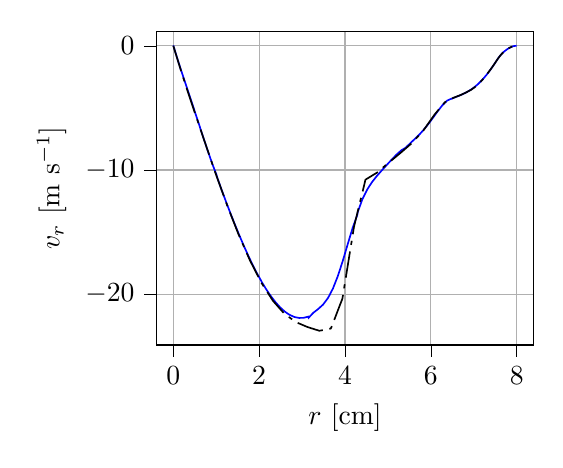
\begin{tikzpicture}

\definecolor{darkgray176}{RGB}{176,176,176}

\begin{axis}[
legend cell align=left,
legend pos= north east,
scale = .7,
ylabel = {$v_r$ [m s$^{-1}$]},
tick align=outside,
xlabel = {$r$ [cm]},
tick pos=left,
x grid style={darkgray176},
xmajorgrids,
xmin=-0.399999991059303, xmax=8.39999981224537,
xtick style={color=black},
y grid style={darkgray176},
ymajorgrids,
ymin=-24.090907088064, ymax=1.17976961811276,
ytick style={color=black}
]
\addplot [semithick, blue]
table {%
0 0.0311024951047235
0.007999999797903 -0.0590078665663074
0.015999999595806 -0.149118228318974
0.023999999393709 -0.239228590153278
0.031999999191612 -0.329338952069222
0.039999998989515 -0.419449314066809
0.047999998787418 -0.509559676146043
0.0560000014957041 -0.599670071088884
0.063999998383224 -0.689780400549457
0.0720000010915101 -0.779890795655602
0.07999999797903 -0.870001125279485
0.0880000006873161 -0.960111520548946
0.095999997574836 -1.05022185033615
0.104000000283122 -1.13876539976559
0.112000002991408 -1.22411329561791
0.119999994058162 -1.30946106726569
0.127999996766448 -1.39480896310393
0.135999999474734 -1.48015685893513
0.14400000218302 -1.5655047547593
0.151999993249774 -1.65085252637892
0.15999999595806 -1.73620042218901
0.167999998666346 -1.82154831799205
0.176000001374632 -1.90689621378805
0.183999992441386 -1.99224398537952
0.191999995149672 -2.07759188116144
0.199999986216426 -2.16293965273882
0.208000000566244 -2.24688572658613
0.215999991632998 -2.33010286763082
0.224000005982816 -2.41332025084126
0.23199999704957 -2.4965373918294
0.239999988116324 -2.57975453278927
0.248000002466142 -2.66297191591489
0.255999993532896 -2.74618905681821
0.26399998459965 -2.82940619769325
0.271999998949468 -2.91262358073404
0.279999990016222 -2.99584072155252
0.28800000436604 -3.07905810453675
0.295999995432794 -3.16227524529867
0.303999986499548 -3.24549238603232
0.312000000849366 -3.3283790415401
0.31999999191612 -3.41126109679376
0.327999982982874 -3.49414315204548
0.335999997332692 -3.57702544851405
0.343999988399446 -3.65990750376188
0.352000002749264 -3.74278980022657
0.359999993816018 -3.82567185547051
0.367999984882772 -3.90855391071251
0.37599999923259 -3.99143620717136
0.383999990299344 -4.07431826240947
0.392000004649162 -4.15720055886444
0.399999972432852 -4.24008237287986
0.40799998678267 -4.323161884834
0.416000001132488 -4.40666830224764
0.423999968916178 -4.49017423364435
0.431999983265996 -4.57368065116504
0.439999997615814 -4.65718706873925
0.448000011965632 -4.74069348636699
0.455999979749322 -4.8241994179778
0.46399999409914 -4.9077058357126
0.472000008448958 -4.99121225350093
0.479999976232648 -5.07471818527234
0.487999990582466 -5.15822460316774
0.496000004932284 -5.24173102111668
0.503999972715974 -5.3252369530487
0.511999987065792 -5.40922515185339
0.52000000141561 -5.49347852958356
0.5279999691993 -5.57773141701435
0.535999983549118 -5.66198479498242
0.543999997898936 -5.74623817306945
0.551999965682626 -5.83049106085711
0.559999980032444 -5.91474443918207
0.567999994382262 -5.99899781762599
0.57600000873208 -6.08325119618888
0.58399997651577 -6.16750408445242
0.591999990865588 -6.25175746325327
0.600000005215406 -6.3360108421731
0.607999972999096 -6.42026373079359
0.615999987348914 -6.50454971687541
0.624000001698732 -6.58883657394501
0.631999969482422 -6.67312294057648
0.63999998383224 -6.75740979799624
0.647999998182058 -6.84169665559108
0.655999965965748 -6.92598302274782
0.663999980315566 -7.01026988069286
0.671999994665384 -7.09455673881301
0.679999962449074 -7.17884310649506
0.687999976798892 -7.26312996496543
0.69599999114871 -7.34741682361092
0.704000005498528 -7.43170368243155
0.711999973282218 -7.5155306128972
0.719999987632036 -7.59830111577292
0.728000001981854 -7.68107161885192
0.735999969765544 -7.76384164034735
0.743999984115362 -7.84661214383294
0.75199999846518 -7.92938264752184
0.75999996624887 -8.01215266962718
0.767999980598688 -8.09492317372271
0.775999994948506 -8.17769367802157
0.784000009298325 -8.26046418252375
0.791999977082014 -8.3432342054424
0.799999944865704 -8.42600422856439
0.808000005781651 -8.50877521546349
0.81599997356534 -8.58907888534641
0.82399994134903 -8.66794640295569
0.832000002264977 -8.74681483889142
0.839999970048666 -8.82568235686868
0.847999937832355 -8.90454987502995
0.855999998748302 -8.98341831151768
0.863999966531992 -9.06228583004696
0.871999934315681 -9.14115334876026
0.879999995231628 -9.22002178580005
0.887999963015318 -9.2988893048814
0.896000023931265 -9.37775774228925
0.903999991714954 -9.45662526173868
0.911999959498644 -9.53549278137216
0.920000020414591 -9.60751405066724
0.92799998819828 -9.67925654232874
0.93599995598197 -9.75099903408878
0.944000016897917 -9.82274236114324
0.951999984681606 -9.89448485310037
0.959999952465296 -9.96622734515603
0.968000013381243 -10.0379706725061
0.975999981164932 -10.1097131647589
0.983999948948622 -10.1814556571102
0.992000009864569 -10.253198984756
0.999999977648258 -10.3249414773045
1.00799994543195 -10.3966839699515
1.01600000634789 -10.5313364862806
1.02399997413158 -10.6090023305273
1.03199994191527 -10.6866681785981
1.04000000283122 -10.7643349346458
1.04799997061491 -10.8420007903631
1.0559999383986 -10.9196666499056
1.06399999931455 -10.997333417417
1.07199996709824 -11.0749992845999
1.07999993488193 -11.1526651556068
1.08799999579787 -11.2303319345752
1.09599996358156 -11.3079978132151
1.10399993136525 -11.385663695673
1.1119999922812 -11.4633304861017
1.11999996006489 -11.5403065203452
1.12800002098083 -11.6152459589493
1.13599998876452 -11.6901845275343
1.14399995654821 -11.7651230985031
1.15200001746416 -11.8400625442587
1.15999998524785 -11.9150011199969
1.16799995303154 -11.9899396981117
1.17600001394749 -12.0648791510157
1.18399998173118 -12.1398177339018
1.19199994951487 -12.2147563191587
1.20000001043081 -12.2896957792055
1.2079999782145 -12.3646343692292
1.21599994599819 -12.4395729616327
1.22400000691414 -12.5139652556505
1.23199997469783 -12.5863696060789
1.23999994248152 -12.6587739586335
1.24800000339746 -12.7311791562151
1.25599997118115 -12.8035835130213
1.26399993896484 -12.8759878719557
1.27199999988079 -12.9483930759098
1.27999996766448 -13.020797439091
1.28799993544817 -13.0932018043998
1.29599999636412 -13.1656070147236
1.30399996414781 -13.2380113842748
1.3119999319315 -13.3104157559488
1.31999999284744 -13.3828209726465
1.32799996063113 -13.4547833002256
1.33599992841482 -13.5247165490808
1.34399998933077 -13.5946506148023
1.35199995711446 -13.6645838691227
1.35999992489815 -13.7345171261749
1.36799998581409 -13.8044512000951
1.37599995359778 -13.8743844626065
1.38400001451373 -13.9443185419854
1.39199998229742 -14.0142518099641
1.39999995008111 -14.0841850806631
1.40800001099706 -14.1541191682295
1.41599997878075 -14.2240524443906
1.42399994656444 -14.2939857232795
1.43200000748038 -14.3635597138873
1.43999997526407 -14.4309550105912
1.44799994304776 -14.498350311184
1.45600000396371 -14.5657464002526
1.4639999717474 -14.6331417086208
1.47199993953109 -14.7005370208789
1.48000000044703 -14.7679331216047
1.48799996823072 -14.8353284416312
1.49599993601441 -14.9027237655456
1.50399999693036 -14.9701198779237
1.51199996471405 -15.0375152096013
1.51999993249774 -15.1049105451613
1.52799999341369 -15.1723066691912
1.53599996119738 -15.2394151594618
1.54399992898107 -15.3040757033358
1.55199998989701 -15.3687370052406
1.5599999576807 -15.4333975596732
1.56800001859665 -15.4980588721347
1.57599989324808 -15.5627186843742
1.58399995416403 -15.6273800073856
1.59200001507998 -15.6920413356753
1.59999988973141 -15.7567011637397
1.60799995064735 -15.8213625025721
1.6160000115633 -15.8860238466808
1.62399988621473 -15.9506836905576
1.63199994713068 -16.0153450452076
1.64000000804663 -16.0797984535917
1.64799988269806 -16.1413967288025
1.65599994361401 -16.2029964448286
1.66400000452995 -16.2645961674499
1.67199987918139 -16.3261944624455
1.67999994009733 -16.3877941982567
1.68800000101328 -16.4493939406532
1.69599987566471 -16.5109922554231
1.70399993658066 -16.5725920110052
1.7119999974966 -16.6341917731683
1.71999987214804 -16.6957901077013
1.72799993306398 -16.7573898830403
1.73599999397993 -16.8189896649636
1.74399986863136 -16.8804791361011
1.75199992954731 -16.9385604710091
1.75999999046326 -16.9966418134447
1.7680000513792 -17.0547231634066
1.77599992603064 -17.1128031685915
1.78399998694658 -17.1708845336046
1.79200004786253 -17.2289659061339
1.79999992251396 -17.2870459338844
1.80799998342991 -17.3451273214592
1.81600004434586 -17.4032087165459
1.82399991899729 -17.4612887668496
1.83199997991323 -17.5193701769712
1.84000004082918 -17.5774515946067
1.84799991548061 -17.6355316674513
1.85599997639656 -17.6895324294955
1.86400003731251 -17.7435086091079
1.87199991196394 -17.7974835397692
1.87999997287989 -17.8514597349211
1.88800003379583 -17.9054359378438
1.89599990844727 -17.9594108918048
1.90399996936321 -18.0133871102552
1.91200003027916 -18.0673633364718
1.91999990493059 -18.1213383137223
1.92799996584654 -18.1753145554587
1.93600002676249 -18.2292908049544
1.94399990141392 -18.2832658054846
1.95199996232986 -18.3372420704942
1.96000002324581 -18.3866031965761
1.96799989789724 -18.4357562678228
1.97599995881319 -18.4849104905407
1.98400001972914 -18.5340647202766
1.99199989438057 -18.5832178125793
1.99999995529652 -18.6323720563444
2.00800001621246 -18.681526307126
2.0159998908639 -18.7306794204697
2.02399995177984 -18.7798336852732
2.03200001269579 -18.8289879570894
2.03999988734722 -18.8781410914609
2.04799994826317 -18.9272953772936
2.05600000917912 -18.9764496701328
2.06399988383055 -19.0400329023105
2.07199994474649 -19.0849877981824
2.08000000566244 -19.1299426484666
2.08799988031387 -19.1748964065249
2.09599994122982 -19.2198511657516
2.10400000214577 -19.2648058795073
2.1119998767972 -19.3097595011573
2.11999993771315 -19.3547141240884
2.12799999862909 -19.3996687016653
2.13599987328053 -19.4446221872557
2.14399993419647 -19.4895766742408
2.15199999511242 -19.5345311159875
2.15999986976385 -19.5794844658666
2.1679999306798 -19.6232317498661
2.17599999159575 -19.6640130597509
2.18399986624718 -19.7047933868567
2.19199992716312 -19.7455746302237
2.19999998807907 -19.786355840374
2.2079998627305 -19.8271360678326
2.21599992364645 -19.8679172116419
2.2239999845624 -19.908698322311
2.23199985921383 -19.9494784503711
2.23999992012978 -19.9902594948628
2.24799998104572 -20.0310405063069
2.25600004196167 -20.0718214847317
2.2639999166131 -20.1126014806673
2.27199997752905 -20.1533823931382
2.280000038445 -20.190996291029
2.28799991309643 -20.2269651406878
2.29599997401237 -20.2629347969782
2.30400003492832 -20.2989044224478
2.31199990957975 -20.3348731796472
2.3199999704957 -20.3708427435544
2.32800003141165 -20.4068122767198
2.33599990606308 -20.4427809416943
2.34399996697903 -20.4787504134532
2.35200002789497 -20.5147198545478
2.35999990254641 -20.5506884275327
2.36799996346235 -20.5866578073774
2.3760000243783 -20.6226271566355
2.38399989902973 -20.658450397545
2.39199995994568 -20.6890685377905
2.40000002086163 -20.7196866426148
2.40799989551306 -20.750303999171
2.415999956429 -20.7809220332432
2.42400001734495 -20.811540031984
2.43199989199638 -20.8421572825488
2.43999995291233 -20.8727752107176
2.44800001382828 -20.9033931036426
2.45599988847971 -20.9340102484844
2.46399994939566 -20.964628071016
2.4720000103116 -20.9952458583948
2.47999988496304 -21.0258628977809
2.48799994587898 -21.0564806149435
2.49600000679493 -21.084804540787
2.50399988144636 -21.1096286907543
2.51199994236231 -21.1344533746443
2.52000000327826 -21.1592780145023
2.52799987792969 -21.1841020323778
2.53599993884563 -21.2089265842841
2.54399999976158 -21.2337510922722
2.55199987441301 -21.2585749783914
2.55999993532896 -21.2833993986421
2.56799999624491 -21.3082237750875
2.57599987089634 -21.3330475297781
2.58399993181229 -21.3578718187147
2.59199999272823 -21.3826960639516
2.59999986737967 -21.4075196875469
2.60799992829561 -21.4276515864119
2.61599998921156 -21.446339298739
2.62399986386299 -21.4650265219033
2.63199992477894 -21.4837141261556
2.63999998569489 -21.5024016764377
2.64799986034632 -21.5210887376968
2.65599992126226 -21.5397761801758
2.66399998217821 -21.5584635688203
2.67199985682964 -21.5771504685809
2.67999991774559 -21.595837749693
2.68799997866154 -21.6145249771057
2.69599985331297 -21.6332117157733
2.70399991422892 -21.6518988359234
2.71199997514486 -21.6697352702382
2.7199998497963 -21.6820404562713
2.72799991071224 -21.6943458660504
2.73599997162819 -21.7066512131204
2.74399984627962 -21.7189562110317
2.75199990719557 -21.7312614328418
2.75999996811152 -21.7435665921028
2.76800002902746 -21.7558716888583
2.77599990367889 -21.7681764366718
2.78399996459484 -21.7804814085878
2.79200002551079 -21.7927863181602
2.79999990016222 -21.8050908789493
2.80799996107817 -21.8173956639918
2.81600002199411 -21.8297003868465
2.82399989664555 -21.8387287401158
2.83199995756149 -21.844505039791
2.84000001847744 -21.8502812719532
2.84799989312887 -21.8560573021737
2.85599995404482 -21.8618333994803
2.86400001496077 -21.8676094294425
2.8719998896122 -21.8733852576362
2.87999995052814 -21.8791611530801
2.88800001144409 -21.8849369813452
2.89599988609552 -21.8907126080152
2.90399994701147 -21.8964883020974
2.91200000792742 -21.9022639291705
2.91999988257885 -21.908039354819
2.9279999434948 -21.9138148480421
2.93600000441074 -21.9138667904316
2.94399987906218 -21.9130655557051
2.95199993997812 -21.912264236477
2.96000000089407 -21.9114628514566
2.9679998755455 -21.9106614193593
2.97599993646145 -21.9098599029195
2.9839999973774 -21.9090583208509
2.99199987202883 -21.9082566918733
2.99999993294477 -21.9074549787117
3.00799999386072 -21.9066532000842
3.01599986851215 -21.9058513747151
3.0239999294281 -21.90504946532
3.03199999034405 -21.9042474906213
3.03999986499548 -21.901888088109
3.04799992591143 -21.8945595469094
3.05599998682737 -21.8872309502795
3.06399986147881 -21.8799024688979
3.07199992239475 -21.8725737615459
3.0799999833107 -21.8652449989009
3.08799985796213 -21.8579163516433
3.09599991887808 -21.8505874785512
3.10399997979403 -21.843258550303
3.11199985444546 -21.8359297375836
3.1199999153614 -21.8286006991596
3.12799997627735 -21.8212716057158
3.1360000371933 -21.8139424572974
3.14400009810925 -21.8066132539498
3.15199978649616 -21.9032075409549
3.15999984741211 -21.8736595871369
3.16799990832806 -21.8441116704785
3.175999969244 -21.8145637908629
3.18400003015995 -21.7850159481736
3.1920000910759 -21.7554681422948
3.19999977946281 -21.7259217490249
3.20799984037876 -21.6963740164196
3.21599990129471 -21.66682632028
3.22399996221066 -21.6372786604922
3.2320000231266 -21.6077310369426
3.24000008404255 -21.5781834495182
3.24799977242947 -21.5486372740104
3.25599983334541 -21.5190897584976
3.26399989426136 -21.4919644579179
3.27199995517731 -21.4705258543757
3.28000001609325 -21.4490872631183
3.2880000770092 -21.4276486841077
3.29599976539612 -21.4062111156091
3.30399982631207 -21.3847725609778
3.31199988722801 -21.36333401848
3.31999994814396 -21.3418954880775
3.32800000905991 -21.3204569697352
3.33600006997585 -21.2990184634138
3.34399975836277 -21.2775809673767
3.35199981927872 -21.2561424849871
3.35999988019466 -21.2347040145085
3.36799994111061 -21.2132655559044
3.37600000202656 -21.1918271091385
3.3840000629425 -21.1667745625999
3.39199975132942 -21.1416885472538
3.39999981224537 -21.1166013681205
3.40799987316132 -21.0915141933906
3.41599993407726 -21.0664270230508
3.42399999499321 -21.0413398570877
3.43200005590916 -21.0162526954869
3.43999974429607 -20.9911667064412
3.44799980521202 -20.9660795535283
3.45599986612797 -20.9409924049391
3.46399992704391 -20.9159052606606
3.47199998795986 -20.8908181206797
3.48000004887581 -20.8657309849834
3.48799973726273 -20.8406450217603
3.49599979817867 -20.80750919015
3.50399985909462 -20.7706245530902
3.51199992001057 -20.7337399229909
3.51999998092651 -20.6968552998311
3.52800004184246 -20.65997068359
3.53600010275841 -20.6230860742467
3.54399979114532 -20.5862031893406
3.55199985206127 -20.5493185937308
3.55999991297722 -20.512434004957
3.56799997389317 -20.4755494229989
3.57600003480911 -20.4386648478359
3.58400009572506 -20.4017802794479
3.59199978411198 -20.3648974353727
3.59999984502792 -20.3280128804738
3.60799990594387 -20.2850181568983
3.61599996685982 -20.2317960554313
3.62400002777576 -20.17857396806
3.63200008869171 -20.1253518947425
3.63999977707863 -20.0721323137633
3.64799983799458 -20.018910268428
3.65599989891052 -19.9656882370221
3.66399995982647 -19.9124662195043
3.67200002074242 -19.8592442158337
3.68000008165836 -19.8060222259694
3.68799977004528 -19.752802728193
3.69599983096123 -19.6995807658188
3.70399989187717 -19.6463588171293
3.71199995279312 -19.5931368820844
3.72000001370907 -19.5387797792122
3.72800007462502 -19.4682888617108
3.73599976301193 -19.3978012473634
3.74399982392788 -19.3273103711828
3.75199988484383 -19.2568195155725
3.75999994575977 -19.1863286804725
3.76800000667572 -19.1158378658228
3.77600006759167 -19.0453470715625
3.78399975597858 -18.9748595800931
3.79199981689453 -18.9043688264366
3.79999987781048 -18.8338780929934
3.80799993872643 -18.7633873797046
3.81599999964237 -18.692896686512
3.82400006055832 -18.6224060133571
3.83199974894524 -18.5519186426333
3.83999980986118 -18.4703759031775
3.84799987077713 -18.3852933270351
3.85599993169308 -18.300210773113
3.86399999260902 -18.2151282413473
3.87200005352497 -18.1300457316741
3.87999974191189 -18.0449672059611
3.88799980282784 -17.9598847402812
3.89599986374378 -17.8748022965036
3.90399992465973 -17.7897198745656
3.91199998557568 -17.7046374744044
3.92000004649162 -17.6195550959577
3.92799973487854 -17.5344767010885
3.93599979579449 -17.4493943658835
3.94399985671043 -17.3643120522071
3.95199991762638 -17.2754991686453
3.95999997854233 -17.1821103558475
3.96800003945827 -17.0887215578886
3.97599972784519 -16.995337123447
3.98399978876114 -16.9019483550387
3.99199984967709 -16.808559601343
3.99999991059303 -16.7151708623183
4.00799997150898 -16.621782137923
4.01600003242493 -16.5283934281155
4.02400009334087 -16.4350047328546
4.03199978172779 -16.3416204008151
4.03999984264374 -16.2482317345235
4.04799990355968 -16.1548430826556
4.05599996447563 -16.0614544451706
4.06400002539158 -15.9682893087688
4.07200008630753 -15.8764879015477
4.07999977469444 -15.784690764189
4.08799983561039 -15.692889347099
4.09599989652634 -15.6010879250951
4.10399995744228 -15.5092864981912
4.11200001835823 -15.4174850664009
4.12000007927418 -15.325683629738
4.12799976766109 -15.2338864630213
4.13599982857704 -15.1420850166542
4.14399988949299 -15.050283565455
4.15199995040894 -14.9584821094375
4.16000001132488 -14.8666806486148
4.16800007224083 -14.7748791830005
4.17599976062775 -14.6830819874145
4.18399982154369 -14.6038411618063
4.19199988245964 -14.5271287773136
4.19999994337559 -14.4504163527785
4.20800000429153 -14.373703888312
4.21600006520748 -14.2969913840245
4.2239997535944 -14.2202824122061
4.23199981451035 -14.1435698286085
4.23999987542629 -14.0668572055191
4.24799993634224 -13.9901445430467
4.25599999725819 -13.9134318412999
4.26400005817413 -13.8367191003868
4.27199974656105 -13.7600098926059
4.279999807477 -13.6832970736846
4.28799986839294 -13.6065842159189
4.29599992930889 -13.3979539059053
4.30399999022484 -13.3213433124581
4.31200005114079 -13.2447328906522
4.3199997395277 -13.1681262083724
4.32799980044365 -13.0915161312629
4.3359998613596 -13.0149062272201
4.34399992227554 -12.9382964967227
4.35199998319149 -12.8616869402513
4.36000004410744 -12.785077558288
4.36799973249435 -12.7084719186798
4.3759997934103 -12.6318628871784
4.38399985432625 -12.5552540316427
4.3919999152422 -12.4786453525619
4.39999997615814 -12.4020368504275
4.40800003707409 -12.3328241017774
4.41599972546101 -12.2771223492983
4.42399978637695 -12.2214180744421
4.4319998472929 -12.1657138713263
4.43999990820885 -12.1100097401517
4.44799996912479 -12.0543056811196
4.45600003004074 -11.9986016944323
4.46399971842766 -11.9429003741867
4.47199977934361 -11.8871965327948
4.47999984025955 -11.8314927643587
4.4879999011755 -11.7757890690834
4.49599996209145 -11.720085447175
4.50400002300739 -11.6643818988402
4.51200008392334 -11.6086784242866
4.51999977231026 -11.5554342703107
4.5279998332262 -11.5131159813907
4.53599989414215 -11.4707977088205
4.5439999550581 -11.4284794526465
4.55200001597404 -11.3861612129151
4.56000007688999 -11.3438429896728
4.56799976527691 -11.3015267535463
4.57599982619286 -11.259208563424
4.5839998871088 -11.2168903899286
4.59199994802475 -11.1745722331124
4.6000000089407 -11.1322540930213
4.60800006985664 -11.089935969703
4.61599975824356 -11.0476198337804
4.62399981915951 -11.0053017441509
4.63199988007545 -10.9629836714383
4.6399999409914 -10.928331809759
4.64800000190735 -10.8935783851136
4.6560000628233 -10.8588249570948
4.66399975121021 -10.8240731440134
4.67199981212616 -10.7893197092189
4.67999987304211 -10.7545662710219
4.68799993395805 -10.7198128294132
4.695999994874 -10.6850593843809
4.70400005578995 -10.6503059359173
4.71199974417686 -10.6155541023332
4.71999980509281 -10.5808006469758
4.72799986600876 -10.5460471881565
4.73599992692471 -10.5112937258653
4.74399998784065 -10.4765402600921
4.7520000487566 -10.4446901123114
4.75999973714352 -10.413380448835
4.76799979805946 -10.3820693290568
4.77599985897541 -10.3507582110084
4.78399991989136 -10.319447094695
4.7919999808073 -10.2881359801215
4.80000004172325 -10.2568248672931
4.80799973011017 -10.225515214241
4.81599979102612 -10.1942041049179
4.82399985194206 -10.1628929973552
4.83199991285801 -10.1315818915582
4.83999997377396 -10.1002707875318
4.8480000346899 -10.0689596852815
4.85599972307682 -10.0376500428378
4.86399978399277 -10.0070244688671
4.87199984490871 -9.97673130412849
4.87999990582466 -9.94643815897422
4.88799996674061 -9.91614503346208
4.89600002765656 -9.8858519276501
4.90399971604347 -9.85556025221709
4.91199977695942 -9.8252671859795
4.91999983787537 -9.79497413961752
4.92799989879131 -9.7646811131901
4.93599995970726 -9.73438810675642
4.94400002062321 -9.70409512037588
4.95199970901012 -9.67380356472309
4.95999976992607 -9.6435106186271
4.96799983084202 -9.61321769276392
4.97599989175797 -9.58307138776582
4.98399995267391 -9.55306958689431
4.99200001358986 -9.52306782256732
4.99999970197678 -9.49306749194702
5.00799976289272 -9.46306580103585
5.01599982380867 -9.43306414699857
5.02399988472462 -9.40306252994587
5.03199994564056 -9.37306094998885
5.04000000655651 -9.34305940723909
5.04800006747246 -9.31305790180858
5.05599975585938 -9.28305783085052
5.06399981677532 -9.25305640039464
5.07199987769127 -9.22305500759676
5.07999993860722 -9.19305365257071
5.08799999952316 -9.16347364374711
5.09600006043911 -9.13473388671208
5.10399974882603 -9.10599550515114
5.11199980974197 -9.07725582260254
5.11999987065792 -9.04851617746777
5.12799993157387 -9.0197765698606
5.13599999248981 -8.99103699989527
5.14400005340576 -8.96229746768648
5.15199974179268 -8.93355931162532
5.15999980270863 -8.90481985527382
5.16799986362457 -8.87608043702577
5.17599992454052 -8.84734105699775
5.18399998545647 -8.81860171530684
5.19200004637241 -8.78986241207056
5.19999973475933 -8.76177020979552
5.20799979567528 -8.73695992764801
5.21599985659122 -8.71214964964972
5.22399991750717 -8.68733937581344
5.23199997842312 -8.66252910615198
5.24000003933907 -8.63771884067823
5.24799972772598 -8.61290973471404
5.25599978864193 -8.58809947765509
5.26399984955788 -8.56328922482133
5.27199991047382 -8.53847897622807
5.27999997138977 -8.5136687318877
5.28800003230572 -8.48885849181344
5.29599972069263 -8.46404941132627
5.30399978160858 -8.43923917982383
5.31199984252453 -8.41442895262743
5.31999990344048 -8.3978694691341
5.32799996435642 -8.3813521964311
5.33600002527237 -8.3648348413466
5.34399971365929 -8.34831817277223
5.35199977457523 -8.33180065215478
5.35999983549118 -8.31528304837988
5.36799989640713 -8.29876536118734
5.37599995732307 -8.28224759031329
5.38400001823902 -8.26572973549666
5.39199970662594 -8.24921256564528
5.39999976754189 -8.23269454215268
5.40799982845783 -8.21617643392116
5.41599988937378 -8.19965824068328
5.42399995028973 -8.18313996217043
5.43200001120567 -8.1417898483455
5.43999969959259 -8.11473293424905
5.44799976050854 -8.0876747417543
5.45599982142448 -8.0606165308294
5.46399988234043 -8.03355830145808
5.47199994325638 -8.00650005362406
5.48000000417233 -7.97944178731141
5.48799969255924 -7.95238476249303
5.49599975347519 -7.92532645917382
5.50399981439114 -7.89826813732652
5.51199987530708 -7.87120979693479
5.51999993622303 -7.8441514379822
5.52799999713898 -7.81709306045234
5.53600005805492 -7.79086521989842
5.54399974644184 -7.76526187337879
5.55199980735779 -7.7396573294033
5.55999986827374 -7.71405278026242
5.56799992918968 -7.68844822595158
5.57599999010563 -7.6628436664662
5.58400005102158 -7.63723910180172
5.59199973940849 -7.61163572425019
5.59999980032444 -7.58603114921387
5.60799986124039 -7.56042656898462
5.61599992215633 -7.53482198355782
5.62399998307228 -7.50921739292887
5.63200004398823 -7.48361279709314
5.63999973237514 -7.45747181401337
5.64799979329109 -7.43017102603976
5.65599985420704 -7.40287023933115
5.66399991512299 -7.37556945388868
5.67199997603893 -7.34826866971347
5.68000003695488 -7.32096788680664
5.6879997253418 -7.29366837645238
5.69599978625774 -7.26636759608977
5.70399984717369 -7.23906681698966
5.71199990808964 -7.21176603916763
5.71999996900558 -7.18446526261964
5.72800002992153 -7.15716448734683
5.73599971830845 -7.12986498463199
5.7439997792244 -7.10234642193487
5.75199984014034 -7.07156884318437
5.75999990105629 -7.0407912670417
5.76799996197224 -7.01001369350921
5.77600002288818 -6.97923612258922
5.7839997112751 -6.94845998746531
5.79199977219105 -6.91768242178109
5.79999983310699 -6.88690485871093
5.80799989402294 -6.8561272982619
5.81599995493889 -6.82534974043937
5.82400001585484 -6.79457218524339
5.83199970424175 -6.76379606585681
5.8399997651577 -6.73301851592085
5.84799982607365 -6.70224096861851
5.85599988698959 -6.66832056437618
5.86399994790554 -6.63365506261467
5.87200000882149 -6.59898956152819
5.8799996972084 -6.56432567534319
5.88799975812435 -6.52966017560856
5.8959998190403 -6.49499467655077
5.90399987995625 -6.4603291781709
5.91199994087219 -6.42566368046819
5.92000000178814 -6.39099818344461
5.92799969017506 -6.35633430132596
5.935999751091 -6.32166880566152
5.94399981200695 -6.28700331067759
5.9519998729229 -6.25233781637477
5.95999993383884 -6.21604909089704
5.96799999475479 -6.17845400979364
5.97599968314171 -6.1408606766684
5.98399974405766 -6.10326559023054
5.9919998049736 -6.06567050112178
5.99999986588955 -6.02807540933973
6.0079999268055 -5.99048031488204
6.01599998772144 -5.95288521774608
6.02400004863739 -5.91529011792966
6.03199973702431 -5.87769676607541
6.03999979794025 -5.8401016608908
6.0479998588562 -5.80250655301839
6.05599991977215 -5.76491144245576
6.0639999806881 -5.72713593927306
6.07200004160404 -5.68893914770821
6.07999972999096 -5.65074412933479
6.08799979090691 -5.61254732682103
6.09599985182285 -5.57435051882525
6.1039999127388 -5.53615370534252
6.11199997365475 -5.49795688636952
6.12000003457069 -5.45976006190334
6.12799972295761 -5.421565010588
6.13599978387356 -5.383368175108
6.14399984478951 -5.34517133411616
6.15199990570545 -5.3069744876075
6.1599999666214 -5.26877763557701
6.16800002753735 -5.23072180338057
6.17599971592426 -5.19562241829648
6.18399977684021 -5.16052139297276
6.19199983775616 -5.12542036191023
6.1999998986721 -5.09031932510368
6.20799995958805 -5.0552182825479
6.216000020504 -5.02011723424259
6.22399970889091 -4.98501781467818
6.23199976980686 -4.94991675484107
6.23999983072281 -4.91481568923635
6.24799989163876 -4.87971461785624
6.2559999525547 -4.84461354069548
6.26399964094162 -4.80951409225804
6.2720000743866 -4.77441136901096
6.27999976277351 -4.74577088849844
6.28800019621849 -4.71883152019213
6.29599988460541 -4.69189465930419
6.30399957299232 -4.66495779704517
6.3120000064373 -4.63801842462513
6.31999969482422 -4.61108155962009
6.3280001282692 -4.58414218445158
6.33599981665611 -4.55720531669519
6.34399950504303 -4.53026844756179
6.35199993848801 -4.50332906826044
6.35999962687492 -4.47639219636846
6.3680000603199 -4.44945281430576
6.37599974870682 -4.42251593965017
6.38400018215179 -4.40341743357836
6.39199987053871 -4.3910796917131
6.39999955892563 -4.37874195963406
6.40799999237061 -4.36640308826597
6.41599968075752 -4.35406537578716
6.4240001142025 -4.34172652403906
6.43199980258942 -4.32938883119642
6.43999949097633 -4.31705114818477
6.44799992442131 -4.30471232593361
6.45599961280823 -4.29237466261214
6.4640000462532 -4.28003586007098
6.47199973464012 -4.26769821647574
6.4800001680851 -4.25535943368074
6.48799985647202 -4.2589210507151
6.49599954485893 -4.2474373898164
6.50399997830391 -4.23595262676962
6.51199966669083 -4.22446890065857
6.5200001001358 -4.21298407238284
6.52799978852272 -4.20150028103889
6.5360002219677 -4.19001538751584
6.54399991035461 -4.17853153092114
6.55199959874153 -4.16704764169545
6.56000003218651 -4.15556265026726
6.56799972057343 -4.14407869576116
6.5760001540184 -4.13259363903745
6.58399984240532 -4.12110961923334
6.59199953079224 -4.10980331486368
6.59999996423721 -4.09861229765189
6.60799965262413 -4.08742230312834
6.61600008606911 -4.07623124691062
6.62399977445602 -4.06504121337827
6.632000207901 -4.05385011814203
6.63999989628792 -4.04266004559007
6.64799958467484 -4.03146995352495
6.65600001811981 -4.02027879974196
6.66399970650673 -4.00908866864015
6.67200013995171 -3.99789747580988
6.67999982833862 -3.98670730565933
6.68799951672554 -3.97551711598124
6.69599995017052 -3.96312491761902
6.70399963855743 -3.95063790743464
6.71200007200241 -3.93814972079236
6.71999976038933 -3.92566268366797
6.7280001938343 -3.91317447007849
6.73599988222122 -3.90068740600699
6.74399957060814 -3.88820032845961
6.75200000405312 -3.87571207443748
6.75999969244003 -3.86322496993119
6.76800012588501 -3.8507366889437
6.77599981427193 -3.83824955746899
6.78399950265884 -3.82576241250941
6.79199993610382 -3.81263418855851
6.79999962449074 -3.79756400431417
6.80800005793571 -3.7824924047395
6.81599974632263 -3.76742219698577
6.82400017976761 -3.75235057389472
6.83199986815453 -3.73728034262267
6.83999955654144 -3.7222100995902
6.84799998998642 -3.70713844121353
6.85599967837334 -3.69206817465398
6.86400011181831 -3.67699649274461
6.87199980020523 -3.6619262026497
6.87999948859215 -3.64685590078638
6.88799992203712 -3.6317841835646
6.89599961042404 -3.61468423109394
6.90400004386902 -3.59604764247645
6.91199973225594 -3.57741277783335
6.92000016570091 -3.55877616601458
6.92799985408783 -3.54014127816759
6.93599954247475 -3.52150637871713
6.94399997591972 -3.50286973208204
6.95199966430664 -3.4842348094185
6.96000009775162 -3.46559813956476
6.96799978613853 -3.44696319368135
6.97599947452545 -3.42832823618395
6.98399990797043 -3.40969153148899
6.99199959635735 -3.39105655076226
7.00000002980232 -3.36864013325693
7.00799971818924 -3.34576387893504
7.01600015163422 -3.32288548379392
7.02399984002113 -3.30000920903025
7.03199952840805 -3.27713292404461
7.03999996185303 -3.25425449823102
7.04799965023994 -3.231378192796
7.05600008368492 -3.20849974652813
7.06399977207184 -3.18562342063775
7.07200020551682 -3.16274495390962
7.07999989390373 -3.13986860755502
7.08799958229065 -3.11699225096944
7.09600001573563 -3.09313172078013
7.10399970412254 -3.06564218452167
7.11200013756752 -3.03815008317975
7.11999982595444 -3.01066053728081
7.12799951434135 -2.9831709865575
7.13599994778633 -2.95567887074761
7.14399963617325 -2.92818931037864
7.15200006961823 -2.90069718492078
7.15999975800514 -2.87320761490332
7.16800019145012 -2.84571547979467
7.17599987983704 -2.81822590012341
7.18399956822395 -2.7907363156267
7.19200000166893 -2.76324416603499
7.19999969005585 -2.7332525398332
7.20800012350082 -2.70107976157783
7.21599981188774 -2.66890998689096
7.22399950027466 -2.63674021961374
7.23199993371964 -2.60456746358457
7.23999962210655 -2.57239771112552
7.24800005555153 -2.54022496992087
7.25599974393845 -2.50805523228709
7.26400017738342 -2.47588250591128
7.27199986577034 -2.44371278310714
7.27999955415726 -2.4115430677157
7.28799998760223 -2.37937036358915
7.29599967598915 -2.34720066303506
7.30400010943413 -2.31122342923658
7.31199979782104 -2.27461147660219
7.31999948620796 -2.23799955326209
7.32799991965294 -2.20138424933419
7.33599960803986 -2.16477238458949
7.34400004148483 -2.12815713927541
7.35199972987175 -2.09154533314767
7.36000016331673 -2.05493014646458
7.36799985170364 -2.01831839897093
7.37599954009056 -1.98170668079944
7.38399997353554 -1.94509158208926
7.39199966192245 -1.90847992257549
7.40000009536743 -1.87116999250929
7.40799978375435 -1.83065900401249
7.41599947214127 -1.79014807918587
7.42399990558624 -1.74963344502917
7.43199959397316 -1.7091226475755
7.44000002741814 -1.6686081408204
7.44799971580505 -1.6280974707793
7.45600014925003 -1.58758309146729
7.46399983763695 -1.54707254887609
7.47199952602386 -1.50656207002089
7.47999995946884 -1.46604788193713
7.48799964785576 -1.42553753058584
7.49600008130074 -1.38502347003959
7.50399976968765 -1.33743496690471
7.51200020313263 -1.29483997396045
7.51999989151955 -1.25254055772489
7.52799957990646 -1.21064939164276
7.53600001335144 -1.16905966391572
7.54399970173836 -1.12808447619982
7.55200013518333 -1.08738919228859
7.55999982357025 -1.04754876392723
7.56799951195717 -1.00793430782279
7.57599994540215 -0.969446575768736
7.58399963378906 -0.93109407882568
7.59200006723404 -0.89418710306828
7.59999975562096 -0.857283564354608
7.60800018906593 -0.822184308154278
7.61599987745285 -0.787088375864456
7.62399956583977 -0.753859971247416
7.63199999928474 -0.720798305120665
7.63999968767166 -0.689631271907235
7.64800012111664 -0.658839698747315
7.65599980950356 -0.629929828964582
7.66399949789047 -0.60164621975348
7.67199993133545 -0.57415506130373
7.67999961972237 -0.547536244586623
7.68800005316734 -0.521968999306093
7.69599974155426 -0.497157034221438
7.70400017499924 -0.473106869098254
7.71199986338615 -0.449822999324604
7.71999955177307 -0.427082268431401
7.72799998521805 -0.405100010653902
7.73599967360497 -0.383497628927795
7.74400010704994 -0.36264905662226
7.75199979543686 -0.342056854395449
7.75999948382378 -0.322228002154948
7.76799991726875 -0.302556681785119
7.77599960565567 -0.283684125914005
7.78400003910065 -0.264888917566211
7.79199972748756 -0.246965527130693
7.80000016093254 -0.229040467384335
7.80799984931946 -0.212113415121207
7.81599953770638 -0.195186342814791
7.82399997115135 -0.179264036111494
7.83199965953827 -0.16343475362883
7.84000009298325 -0.148694104611109
7.84799978137016 -0.134116899647636
7.85599946975708 -0.120569618791767
7.86399990320206 -0.107364484088519
7.87199959158897 -0.0951433929610183
7.88000002503395 -0.0834126726873721
7.88799971342087 -0.0725870689839688
7.89600014686584 -0.0624062823870449
7.90399983525276 -0.0530263393305335
7.91199952363968 -0.044446295282119
7.91999995708466 -0.0365422676184619
7.92799964547157 -0.029586540022834
7.93600007891655 -0.0231713240316846
7.94399976730347 -0.017838961425308
7.95199945569038 -0.0129057344878322
7.95999988913536 -0.00916993907301763
7.96799957752228 -0.00569191634323959
7.97600001096725 -0.00350124674672206
7.98399969935417 -0.00143302862221988
7.99200013279915 -0.000710062589697796
7.99999982118607 1.28361150130952e-05
};
\addplot [semithick, black, dash pattern=on 9.6pt off 2.4pt on 1.5pt off 2.4pt]
table {%
0 9.90432935927652e-15
0.00800800800800801 -0.0893684102283467
0.016016016016016 -0.178736820456703
0.024024024024024 -0.26810523068506
0.032032032032032 -0.357681639592509
0.04004004004004 -0.447374284753609
0.048048048048048 -0.53706692991471
0.0560560560560561 -0.62675957507581
0.0640640640640641 -0.71645222023691
0.0720720720720721 -0.80614486539801
0.0800800800800801 -0.895837510559111
0.0880880880880881 -0.985530155720211
0.0960960960960961 -1.07522280088131
0.104104104104104 -1.16491544604241
0.112112112112112 -1.25460809120351
0.12012012012012 -1.34430073636461
0.128128128128128 -1.43399338152571
0.136136136136136 -1.52368602668681
0.144144144144144 -1.61337867184791
0.152152152152152 -1.70307131700901
0.16016016016016 -1.79276396217011
0.168168168168168 -1.88245660733121
0.176176176176176 -1.97202491074997
0.184184184184184 -2.06139332097832
0.192192192192192 -2.15076173120668
0.2002002002002 -2.23999350248193
0.208208208208208 -2.32389609523345
0.216216216216216 -2.40779868798496
0.224224224224224 -2.49170128073648
0.232232232232232 -2.57560387348799
0.24024024024024 -2.65981401327539
0.248248248248248 -2.74402575864854
0.256256256256256 -2.82823750402169
0.264264264264264 -2.91244924939485
0.272272272272272 -2.996660994768
0.28028028028028 -3.08087274014115
0.288288288288288 -3.16508448551431
0.296296296296296 -3.24929623088746
0.304304304304304 -3.33350797626061
0.312312312312312 -3.41771972163377
0.32032032032032 -3.50193146700692
0.328328328328328 -3.58614321238007
0.336336336336336 -3.67035495775322
0.344344344344344 -3.75456670312638
0.352352352352352 -3.83877844849953
0.36036036036036 -3.92299019387268
0.368368368368368 -4.00720193924584
0.376376376376376 -4.09141368461899
0.384384384384384 -4.17562542999214
0.392392392392392 -4.2598371753653
0.4004004004004 -4.34404892073845
0.408408408408408 -4.42823432859081
0.416416416416416 -4.51213692134232
0.424424424424424 -4.59603951409383
0.432432432432432 -4.67994210684535
0.44044044044044 -4.76370000098685
0.448448448448448 -4.84497172416133
0.456456456456456 -4.92624344733581
0.464464464464464 -5.00751517051029
0.472472472472473 -5.08878689368477
0.48048048048048 -5.17022078258352
0.488488488488488 -5.25179519355508
0.496496496496497 -5.33336960452663
0.504504504504504 -5.41494401549818
0.512512512512513 -5.49651842646973
0.520520520520521 -5.57809283744129
0.528528528528528 -5.65966724841284
0.536536536536537 -5.74124165938439
0.544544544544545 -5.82281607035594
0.552552552552553 -5.9043904813275
0.560560560560561 -5.98596489229905
0.568568568568569 -6.0675393032706
0.576576576576577 -6.14911371424215
0.584584584584585 -6.23068812521371
0.592592592592593 -6.31226253618526
0.600600600600601 -6.39383694715681
0.608608608608609 -6.47541135812836
0.616616616616617 -6.55698576909992
0.624624624624625 -6.63856018007147
0.632632632632633 -6.72013459104302
0.640640640640641 -6.80170900201457
0.648648648648649 -6.88328341298613
0.656656656656657 -6.96485782395768
0.664664664664665 -7.04643223492923
0.672672672672673 -7.12800664590078
0.680680680680681 -7.2092882209571
0.688688688688689 -7.29055994413159
0.696696696696697 -7.37183166730606
0.704704704704705 -7.45310339048055
0.712712712712713 -7.53400541399743
0.720720720720721 -7.61445229057767
0.728728728728729 -7.6948991671579
0.736736736736737 -7.77534604373814
0.744744744744745 -7.85579292031837
0.752752752752753 -7.93652098062741
0.760760760760761 -8.01727054500471
0.768768768768769 -8.09802010938202
0.776776776776777 -8.17876967375933
0.784784784784785 -8.25951923813664
0.792792792792793 -8.34026880251395
0.800800800800801 -8.42101836689125
0.808808808808809 -8.50176793126856
0.816816816816817 -8.58251749564587
0.824824824824825 -8.66326706002318
0.832832832832833 -8.74401662440049
0.840840840840841 -8.82476618877779
0.848848848848849 -8.9055157531551
0.856856856856857 -8.98626531753241
0.864864864864865 -9.06701488190972
0.872872872872873 -9.14776444628703
0.880880880880881 -9.22851401066434
0.888888888888889 -9.30926357504164
0.896896896896897 -9.39001313941895
0.904904904904905 -9.47076270379626
0.912912912912913 -9.55151226817357
0.920920920920921 -9.63226183255087
0.928928928928929 -9.71301139692818
0.936936936936937 -9.79376096130549
0.944944944944945 -9.87440135956012
0.952952952952953 -9.95484823614036
0.960960960960961 -10.0352951127206
0.968968968968969 -10.1157419893008
0.976976976976977 -10.1961888658811
0.984984984984985 -10.2731292621897
0.992992992992993 -10.3494087427461
1.001001001001 -10.4256882233025
1.00900900900901 -10.5019677038589
1.01701701701702 -10.5783409229185
1.02502502502503 -10.6549113714461
1.03303303303303 -10.7314818199736
1.04104104104104 -10.8080522685011
1.04904904904905 -10.8846227170287
1.05705705705706 -10.9611931655562
1.06506506506507 -11.0377636140837
1.07307307307307 -11.1143340626113
1.08108108108108 -11.1909045111388
1.08908908908909 -11.2674749596663
1.0970970970971 -11.3440454081939
1.10510510510511 -11.4206158567214
1.11311311311311 -11.4971863052489
1.12112112112112 -11.5737567537765
1.12912912912913 -11.650327202304
1.13713713713714 -11.7268976508315
1.14514514514515 -11.8034680993591
1.15315315315315 -11.8800385478866
1.16116116116116 -11.9566089964141
1.16916916916917 -12.0331794449417
1.17717717717718 -12.1097498934692
1.18518518518519 -12.1863203419967
1.19319319319319 -12.2628907905243
1.2012012012012 -12.3394612390518
1.20920920920921 -12.4160316875793
1.21721721721722 -12.4923827856195
1.22522522522523 -12.5686622661759
1.23323323323323 -12.6449417467323
1.24124124124124 -12.7212212272886
1.24924924924925 -12.7961404134932
1.25725725725726 -12.8666219737744
1.26526526526527 -12.9371035340555
1.27327327327327 -13.0075850943367
1.28128128128128 -13.0780666546178
1.28928928928929 -13.1487393429518
1.2972972972973 -13.2194880767296
1.30530530530531 -13.2902368105075
1.31331331331331 -13.3609855442853
1.32132132132132 -13.4317342780632
1.32932932932933 -13.502483011841
1.33733733733734 -13.5732317456189
1.34534534534535 -13.6439804793967
1.35335335335335 -13.7147292131746
1.36136136136136 -13.7854779469524
1.36936936936937 -13.8562266807303
1.37737737737738 -13.9269754145081
1.38538538538539 -13.997724148286
1.39339339339339 -14.0684728820639
1.4014014014014 -14.1392216158417
1.40940940940941 -14.2099703496196
1.41741741741742 -14.2807190833974
1.42542542542543 -14.3514678171753
1.43343343343343 -14.4222165509531
1.44144144144144 -14.492965284731
1.44944944944945 -14.5637140185088
1.45745745745746 -14.6344627522867
1.46546546546547 -14.7052114860645
1.47347347347347 -14.7759602198424
1.48148148148148 -14.8466696592455
1.48948948948949 -14.9171512195267
1.4974974974975 -14.9876327798079
1.50550550550551 -15.058114340089
1.51351351351351 -15.1285959003702
1.52152152152152 -15.1944084423251
1.52952952952953 -15.2574532148464
1.53753753753754 -15.3204979873676
1.54554554554555 -15.3835427598889
1.55355355355355 -15.4466127676616
1.56156156156156 -15.5098899513287
1.56956956956957 -15.5731671349958
1.57757757757758 -15.6364443186629
1.58558558558559 -15.69972150233
1.59359359359359 -15.7629986859971
1.6016016016016 -15.8262758696642
1.60960960960961 -15.8895530533313
1.61761761761762 -15.9528302369984
1.62562562562563 -16.0161074206655
1.63363363363363 -16.0793846043326
1.64164164164164 -16.1426617879996
1.64964964964965 -16.2059389716667
1.65765765765766 -16.2692161553338
1.66566566566567 -16.3324933390009
1.67367367367367 -16.395770522668
1.68168168168168 -16.4590477063351
1.68968968968969 -16.5223248900022
1.6976976976977 -16.5856020736693
1.70570570570571 -16.6488792573364
1.71371371371371 -16.7121564410035
1.72172172172172 -16.7754336246706
1.72972972972973 -16.8387108083377
1.73773773773774 -16.9019879920048
1.74574574574575 -16.9652651756719
1.75375375375375 -17.0284167913085
1.76176176176176 -17.0914615638298
1.76976976976977 -17.154506336351
1.77777777777778 -17.2175511088723
1.78578578578579 -17.2804028636136
1.79379379379379 -17.3342724567925
1.8018018018018 -17.3881420499715
1.80980980980981 -17.4420116431504
1.81781781781782 -17.4958812363294
1.82582582582583 -17.5498452371095
1.83383383383383 -17.6039029725795
1.84184184184184 -17.6579607080494
1.84984984984985 -17.7120184435194
1.85785785785786 -17.7660761789894
1.86586586586587 -17.8201339144594
1.87387387387387 -17.8741916499294
1.88188188188188 -17.9282493853994
1.88988988988989 -17.9823071208693
1.8978978978979 -18.0363648563393
1.90590590590591 -18.0904225918093
1.91391391391391 -18.1444803272793
1.92192192192192 -18.1985380627493
1.92992992992993 -18.2525957982193
1.93793793793794 -18.3066535336892
1.94594594594595 -18.3607112691592
1.95395395395395 -18.4147690046292
1.96196196196196 -18.4688267400992
1.96996996996997 -18.5228844755692
1.97797797797798 -18.5769422110391
1.98598598598599 -18.6309999465091
1.99399399399399 -18.6850576819791
2.002002002002 -18.7391154174491
2.01001001001001 -18.7931731529191
2.01801801801802 -18.8472308883891
2.02602602602603 -18.9011129961121
2.03403403403403 -18.954982589291
2.04204204204204 -19.00885218247
2.05005005005005 -19.0627217756489
2.05805805805806 -19.1121173876338
2.06606606606607 -19.1551863930782
2.07407407407407 -19.1982553985225
2.08208208208208 -19.2413244039669
2.09009009009009 -19.2843934094112
2.0980980980981 -19.3275909003149
2.10610610610611 -19.3708034671243
2.11411411411411 -19.4140160339337
2.12212212212212 -19.4572286007431
2.13013013013013 -19.5004411675525
2.13813813813814 -19.5436537343619
2.14614614614615 -19.5868663011713
2.15415415415415 -19.6300788679807
2.16216216216216 -19.6732914347901
2.17017017017017 -19.7165040015995
2.17817817817818 -19.7597165684089
2.18618618618619 -19.8029291352184
2.19419419419419 -19.8461417020278
2.2022022022022 -19.8893542688372
2.21021021021021 -19.9325668356466
2.21821821821822 -19.975779402456
2.22622622622623 -20.0189919692654
2.23423423423423 -20.0622045360748
2.24224224224224 -20.1054171028842
2.25025025025025 -20.1486296696936
2.25825825825826 -20.191842236503
2.26626626626627 -20.2350548033124
2.27427427427427 -20.2782673701218
2.28228228228228 -20.3214799369312
2.29029029029029 -20.3646456048775
2.2982982982983 -20.4077146103219
2.30630630630631 -20.4507836157662
2.31431431431431 -20.4938526212106
2.32232232232232 -20.5369216266549
2.33033033033033 -20.5703694916792
2.33833833833834 -20.601522783498
2.34634634634635 -20.6326760753168
2.35435435435435 -20.6638293671356
2.36236236236236 -20.6950181761074
2.37037037037037 -20.7262947111442
2.37837837837838 -20.757571246181
2.38638638638639 -20.7888477812178
2.39439439439439 -20.8201243162546
2.4024024024024 -20.8514008512914
2.41041041041041 -20.8826773863283
2.41841841841842 -20.9139539213651
2.42642642642643 -20.9452304564019
2.43443443443443 -20.9765069914387
2.44244244244244 -21.0077835264755
2.45045045045045 -21.0390600615123
2.45845845845846 -21.0703365965491
2.46646646646647 -21.1016131315859
2.47447447447447 -21.1328896666228
2.48248248248248 -21.1641662016596
2.49049049049049 -21.1954427366964
2.4984984984985 -21.2267192717332
2.50650650650651 -21.25799580677
2.51451451451451 -21.2892723418068
2.52252252252252 -21.3205488768436
2.53053053053053 -21.3518254118805
2.53853853853854 -21.3831019469173
2.54654654654655 -21.4143784819541
2.55455455455455 -21.4456550169909
2.56256256256256 -21.4768428292591
2.57057057057057 -21.5079961210779
2.57857857857858 -21.5391494128967
2.58658658658659 -21.5703027047155
2.59459459459459 -21.5991384850243
2.6026026026026 -21.618742003673
2.61061061061061 -21.6383455223217
2.61861861861862 -21.6579490409704
2.62662662662663 -21.6775525596191
2.63463463463463 -21.6972770089499
2.64264264264264 -21.71705799998
2.65065065065065 -21.73683899101
2.65865865865866 -21.75661998204
2.66666666666667 -21.77640097307
2.67467467467467 -21.7961819641001
2.68268268268268 -21.8159629551301
2.69069069069069 -21.8357439461601
2.6986986986987 -21.8555249371901
2.70670670670671 -21.8753059282201
2.71471471471471 -21.8950869192502
2.72272272272272 -21.9148679102802
2.73073073073073 -21.9346489013102
2.73873873873874 -21.9544298923402
2.74674674674675 -21.9742108833703
2.75475475475475 -21.9939918744003
2.76276276276276 -22.0137728654303
2.77077077077077 -22.0335538564603
2.77877877877878 -22.0533348474904
2.78678678678679 -22.0731158385204
2.7947947947948 -22.0928968295504
2.8028028028028 -22.1126778205804
2.81081081081081 -22.1324588116105
2.81881881881882 -22.1522398026405
2.82682682682683 -22.172000721374
2.83483483483483 -22.1916042400227
2.84284284284284 -22.2112077586714
2.85085085085085 -22.2308112773201
2.85885885885886 -22.2504147959688
2.86686686686687 -22.2651984124926
2.87487487487487 -22.2766855998416
2.88288288288288 -22.2881727871905
2.89089089089089 -22.2996599745395
2.8988988988989 -22.3111713990198
2.90690690690691 -22.3229834512916
2.91491491491492 -22.3347955035635
2.92292292292292 -22.3466075558353
2.93093093093093 -22.3584196081071
2.93893893893894 -22.3702316603789
2.94694694694695 -22.3820437126507
2.95495495495495 -22.3938557649225
2.96296296296296 -22.4056678171943
2.97097097097097 -22.4174798694661
2.97897897897898 -22.4292919217379
2.98698698698699 -22.4411039740098
2.994994994995 -22.4529160262816
3.003003003003 -22.4647280785534
3.01101101101101 -22.4765401308252
3.01901901901902 -22.488352183097
3.02702702702703 -22.5001642353688
3.03503503503504 -22.5119762876406
3.04304304304304 -22.5237883399124
3.05105105105105 -22.5356003921842
3.05905905905906 -22.5474124444561
3.06706706706707 -22.5592244967279
3.07507507507508 -22.5710365489997
3.08308308308308 -22.5828486012715
3.09109109109109 -22.5946606535433
3.0990990990991 -22.6063082204941
3.10710710710711 -22.6177954078431
3.11511511511512 -22.629282595192
3.12312312312312 -22.640769782541
3.13113113113113 -22.65225696989
3.13913913913914 -22.6608246323975
3.14714714714715 -22.6693540617428
3.15515515515516 -22.6778834910881
3.16316316316316 -22.6864129204334
3.17117117117117 -22.6950323720631
3.17917917917918 -22.7037542286898
3.18718718718719 -22.7124760853165
3.1951951951952 -22.7211979419432
3.2032032032032 -22.7299197985699
3.21121121121121 -22.7386416551966
3.21921921921922 -22.7473635118233
3.22722722722723 -22.75608536845
3.23523523523523 -22.7648072250767
3.24324324324324 -22.7735290817034
3.25125125125125 -22.7822509383301
3.25925925925926 -22.7909727949568
3.26726726726727 -22.7996946515835
3.27527527527528 -22.8084165082102
3.28328328328328 -22.8171383648369
3.29129129129129 -22.8258602214636
3.2992992992993 -22.8345820780903
3.30730730730731 -22.843303934717
3.31531531531532 -22.8520257913437
3.32332332332332 -22.8607476479704
3.33133133133133 -22.8694695045971
3.33933933933934 -22.8781913612238
3.34734734734735 -22.8869132178505
3.35535535535536 -22.8956350744772
3.36336336336336 -22.9043569311039
3.37137137137137 -22.9129056954902
3.37937937937938 -22.9214351248355
3.38738738738739 -22.9299645541808
3.3953953953954 -22.9384939835262
3.4034034034034 -22.942239965056
3.41141141141141 -22.9381903654116
3.41941941941942 -22.9341407657672
3.42742742742743 -22.9300911661228
3.43543543543544 -22.9260415664783
3.44344344344344 -22.9207225186097
3.45145145145145 -22.9151985701371
3.45945945945946 -22.9096746216645
3.46746746746747 -22.9041506731919
3.47547547547548 -22.8986267247193
3.48348348348348 -22.8931027762466
3.49149149149149 -22.887578827774
3.4994994994995 -22.8820548793014
3.50750750750751 -22.8765309308288
3.51551551551552 -22.8710069823562
3.52352352352352 -22.8654830338836
3.53153153153153 -22.859959085411
3.53953953953954 -22.8544351369384
3.54754754754755 -22.8489111884658
3.55555555555556 -22.8433872399932
3.56356356356356 -22.8378632915206
3.57157157157157 -22.8323393430479
3.57957957957958 -22.8268153945753
3.58758758758759 -22.8212914461027
3.5955955955956 -22.8157674976301
3.6036036036036 -22.8102435491575
3.61161161161161 -22.8047196006849
3.61961961961962 -22.7991956522123
3.62762762762763 -22.7936717037397
3.63563563563564 -22.7885793241465
3.64364364364364 -22.7845297245021
3.65165165165165 -22.7804801248576
3.65965965965966 -22.7764305252132
3.66766766766767 -22.7723809255688
3.67567567567568 -22.7193795599907
3.68368368368368 -22.6520414192315
3.69169169169169 -22.5847032784723
3.6996996996997 -22.5173651377132
3.70770770770771 -22.4487448862431
3.71571571571572 -22.3763634537422
3.72372372372372 -22.3039820212413
3.73173173173173 -22.2316005887404
3.73973973973974 -22.1592191562395
3.74774774774775 -22.0868377237385
3.75575575575576 -22.0144562912376
3.76376376376376 -21.9420748587367
3.77177177177177 -21.8696934262358
3.77977977977978 -21.7973119937349
3.78778778778779 -21.7249305612339
3.7957957957958 -21.652549128733
3.8038038038038 -21.5801676962321
3.81181181181181 -21.5077862637312
3.81981981981982 -21.4354048312303
3.82782782782783 -21.3630233987293
3.83583583583584 -21.2906419662284
3.84384384384384 -21.2182605337275
3.85185185185185 -21.1458791012266
3.85985985985986 -21.0734976687257
3.86786786786787 -21.0011162362247
3.87587587587588 -20.9287348037238
3.88388388388388 -20.8563533712229
3.89189189189189 -20.783971938722
3.8998998998999 -20.7115905062211
3.90790790790791 -20.6426683498534
3.91591591591592 -20.5753302090942
3.92392392392392 -20.5079920683351
3.93193193193193 -20.4406539275759
3.93993993993994 -20.3558102155715
3.94794794794795 -20.1834392855147
3.95595595595596 -20.0110683554579
3.96396396396396 -19.8386974254012
3.97197197197197 -19.6663264953444
3.97997997997998 -19.4944623315979
3.98798798798799 -19.3228741500909
3.995995995996 -19.1512859685839
4.004004004004 -18.9796977870768
4.01201201201201 -18.8081096055698
4.02002002002002 -18.6365214240628
4.02802802802803 -18.4649332425558
4.03603603603604 -18.2933450610488
4.04404404404404 -18.1217568795417
4.05205205205205 -17.9501686980347
4.06006006006006 -17.7785805165277
4.06806806806807 -17.6069923350207
4.07607607607608 -17.4354041535136
4.08408408408408 -17.2638159720066
4.09209209209209 -17.0922277904996
4.1001001001001 -16.9206396089926
4.10810810810811 -16.7490514274855
4.11611611611612 -16.5774632459785
4.12412412412412 -16.4058750644715
4.13213213213213 -16.2342868829645
4.14014014014014 -16.0626987014574
4.14814814814815 -15.8911105199504
4.15615615615616 -15.7195223384434
4.16416416416416 -15.5479341569364
4.17217217217217 -15.3762840487862
4.18018018018018 -15.2039131187294
4.18818818818819 -15.0315421886727
4.1961961961962 -14.8591712586159
4.2042042042042 -14.6868003285591
4.21221221221221 -14.5453373522412
4.22022022022022 -14.4281724357442
4.22822822822823 -14.3110075192473
4.23623623623624 -14.1938426027504
4.24424424424424 -14.0768489418094
4.25225225225225 -13.9639003706736
4.26026026026026 -13.8509517995379
4.26826826826827 -13.7380032284021
4.27627627627628 -13.6250546572664
4.28428428428428 -13.5121060861306
4.29229229229229 -13.3991575149948
4.3003003003003 -13.2862089438591
4.30830830830831 -13.1732603727233
4.31631631631632 -13.0603118015876
4.32432432432432 -12.9473632304518
4.33233233233233 -12.8344146593161
4.34034034034034 -12.7214660881803
4.34834834834835 -12.6085175170446
4.35635635635636 -12.4955689459088
4.36436436436436 -12.3826203747731
4.37237237237237 -12.2696718036373
4.38038038038038 -12.1567232325015
4.38838838838839 -12.0437746613658
4.3963963963964 -11.93082609023
4.4044044044044 -11.8178775190943
4.41241241241241 -11.7049289479585
4.42042042042042 -11.5919803768228
4.42842842842843 -11.479031805687
4.43643643643644 -11.3660832345513
4.44444444444444 -11.2511432313163
4.45245245245245 -11.1339783148193
4.46046046046046 -11.0168133983224
4.46846846846847 -10.8996484818255
4.47647647647648 -10.7824835653285
4.48448448448448 -10.7611118567698
4.49249249249249 -10.7444577505373
4.5005005005005 -10.7278036443047
4.50850850850851 -10.7111495380722
4.51651651651652 -10.6944059203963
4.52452452452453 -10.6775454816612
4.53253253253253 -10.6606850429261
4.54054054054054 -10.6438246041911
4.54854854854855 -10.626964165456
4.55655655655656 -10.6101037267209
4.56456456456456 -10.5932432879858
4.57257257257257 -10.5763828492507
4.58058058058058 -10.5595224105157
4.58858858858859 -10.5426619717806
4.5965965965966 -10.5258015330455
4.6046046046046 -10.5089410943104
4.61261261261261 -10.4920806555754
4.62062062062062 -10.4752202168403
4.62862862862863 -10.4583597781052
4.63663663663664 -10.4414993393701
4.64464464464465 -10.4246389006351
4.65265265265265 -10.4077784619
4.66066066066066 -10.3909180231649
4.66866866866867 -10.3740575844298
4.67667667667668 -10.3571971456947
4.68468468468468 -10.3403367069597
4.69269269269269 -10.3234762682246
4.7007007007007 -10.3066158294895
4.70870870870871 -10.2897553907544
4.71671671671672 -10.2730735432546
4.72472472472472 -10.256419437022
4.73273273273273 -10.2397653307895
4.74074074074074 -10.2231112245569
4.74874874874875 -10.2041162648748
4.75675675675676 -10.1807027087568
4.76476476476477 -10.1572891526388
4.77277277277277 -10.1338755965208
4.78078078078078 -10.1104620404027
4.78878878878879 -10.0868266945034
4.7967967967968 -10.0631449717715
4.8048048048048 -10.0394632490395
4.81281281281281 -10.0157815263076
4.82082082082082 -9.99209980357561
4.82882882882883 -9.96841808084366
4.83683683683684 -9.94473635811172
4.84484484484485 -9.92105463537977
4.85285285285285 -9.89737291264782
4.86086086086086 -9.87369118991588
4.86886886886887 -9.85000946718393
4.87687687687688 -9.82632774445198
4.88488488488489 -9.80264602172004
4.89289289289289 -9.77896429898809
4.9009009009009 -9.75528257625614
4.90890890890891 -9.73160085352419
4.91691691691692 -9.70791913079225
4.92492492492492 -9.6842374080603
4.93293293293293 -9.66055568532836
4.94094094094094 -9.63687396259641
4.94894894894895 -9.61319223986446
4.95695695695696 -9.58951051713251
4.96496496496497 -9.56582879440057
4.97297297297297 -9.54214707166862
4.98098098098098 -9.51853473837522
4.98898898898899 -9.49512118225719
4.996996996997 -9.47170762613917
5.00500500500501 -9.44829407002114
5.01301301301301 -9.42488051390312
5.02102102102102 -9.40208303316006
5.02902902902903 -9.37950256713391
5.03703703703704 -9.35692210110776
5.04504504504504 -9.33434163508161
5.05305305305305 -9.3116945872661
5.06106106106106 -9.28881183077912
5.06906906906907 -9.26592907429215
5.07707707707708 -9.24304631780518
5.08508508508509 -9.2201635613182
5.09309309309309 -9.19728080483123
5.1011011011011 -9.17439804834425
5.10910910910911 -9.15151529185728
5.11711711711712 -9.1286325353703
5.12512512512513 -9.10574977888333
5.13313313313313 -9.08286702239635
5.14114114114114 -9.05998426590938
5.14914914914915 -9.0371015094224
5.15715715715716 -9.01421875293543
5.16516516516516 -8.99133599644846
5.17317317317317 -8.96845323996148
5.18118118118118 -8.94557048347451
5.18918918918919 -8.92268772698753
5.1971971971972 -8.89980497050056
5.20520520520521 -8.87692221401358
5.21321321321321 -8.85403945752661
5.22122122122122 -8.83115670103964
5.22922922922923 -8.80827394455266
5.23723723723724 -8.78539118806568
5.24524524524525 -8.76250843157871
5.25325325325325 -8.73982275425713
5.26126126126126 -8.71724228823097
5.26926926926927 -8.69466182220483
5.27727727727728 -8.67208135617868
5.28528528528528 -8.64932996584629
5.29329329329329 -8.62546149131686
5.3013013013013 -8.60159301678742
5.30930930930931 -8.57772454225799
5.31731731731732 -8.55385606772856
5.32532532532533 -8.52991398224776
5.33333333333333 -8.50592551380013
5.34134134134134 -8.4819370453525
5.34934934934935 -8.45794857690487
5.35735735735736 -8.43396010845724
5.36536536536537 -8.40997164000961
5.37337337337337 -8.38598317156199
5.38138138138138 -8.36199470311436
5.38938938938939 -8.33800623466673
5.3973973973974 -8.3140177662191
5.40540540540541 -8.29002929777147
5.41341341341341 -8.26604082932384
5.42142142142142 -8.24205236087621
5.42942942942943 -8.21806389242858
5.43743743743744 -8.19407542398096
5.44544544544545 -8.17008695553332
5.45345345345345 -8.1460984870857
5.46146146146146 -8.12211001863807
5.46946946946947 -8.09812155019044
5.47747747747748 -8.07413308174281
5.48548548548549 -8.05014461329518
5.49349349349349 -8.02615614484755
5.5015015015015 -8.00216767639992
5.50950950950951 -7.9781792079523
5.51751751751752 -7.95419615735028
5.52552552552553 -7.93032768282085
5.53353353353353 -7.90645920829142
5.54154154154154 -7.88259073376199
5.54954954954955 -7.85872225923256
5.55755755755756 -7.83154312199396
5.56556556556557 -7.80137944329705
5.57357357357357 -7.77121576460015
5.58158158158158 -7.74105208590324
5.58958958958959 -7.7108886357671
5.5975975975976 -7.68075930793646
5.60560560560561 -7.65062998010581
5.61361361361361 -7.62050065227517
5.62162162162162 -7.59037132444452
5.62962962962963 -7.56024199661387
5.63763763763764 -7.53011266878322
5.64564564564565 -7.49998334095258
5.65365365365365 -7.46985401312193
5.66166166166166 -7.43972468529128
5.66966966966967 -7.40959535746064
5.67767767767768 -7.37946602962999
5.68568568568569 -7.34933670179934
5.69369369369369 -7.3192073739687
5.7017017017017 -7.28907804613805
5.70970970970971 -7.2589487183074
5.71771771771772 -7.22881939047676
5.72572572572573 -7.19869006264611
5.73373373373373 -7.16856073481546
5.74174174174174 -7.13843140698482
5.74974974974975 -7.10830207915417
5.75775775775776 -7.07817275132352
5.76576576576577 -7.04804342349288
5.77377377377377 -7.01791409566223
5.78178178178178 -6.98778476783158
5.78978978978979 -6.95764038233209
5.7977977977978 -6.92747670363519
5.80580580580581 -6.89731302493828
5.81381381381381 -6.86714934624137
5.82182182182182 -6.83698566754447
5.82982982982983 -6.79823810458438
5.83783783783784 -6.75873498438665
5.84584584584585 -6.71923186418893
5.85385385385385 -6.6797287439912
5.86186186186186 -6.64030621699665
5.86986986986987 -6.60100465451501
5.87787787787788 -6.56170309203337
5.88588588588589 -6.52240152955173
5.89389389389389 -6.48309996707009
5.9019019019019 -6.44379840458845
5.90990990990991 -6.40449684210682
5.91791791791792 -6.36519527962518
5.92592592592593 -6.32589371714354
5.93393393393393 -6.2865921546619
5.94194194194194 -6.24729059218026
5.94994994994995 -6.20798902969862
5.95795795795796 -6.16868746721699
5.96596596596597 -6.12938590473535
5.97397397397397 -6.09008434225371
5.98198198198198 -6.05078277977207
5.98998998998999 -6.01148121729043
5.997997997998 -5.97217965480879
6.00600600600601 -5.93287809232716
6.01401401401401 -5.89357652984552
6.02202202202202 -5.85427496736388
6.03003003003003 -5.81497340488224
6.03803803803804 -5.7756718424006
6.04604604604605 -5.73637027991897
6.05405405405405 -5.69706871743732
6.06206206206206 -5.65759955023056
6.07007007007007 -5.61809643003284
6.07807807807808 -5.57859330983511
6.08608608608609 -5.53909018963738
6.09409409409409 -5.50162185677123
6.1021021021021 -5.46863425912744
6.11011011011011 -5.43564666148366
6.11811811811812 -5.40265906383987
6.12612612612613 -5.36973127546117
6.13413413413413 -5.3369365405229
6.14214214214214 -5.30414180558464
6.15015015015015 -5.27134707064638
6.15815815815816 -5.23855233570812
6.16616616616617 -5.20575760076986
6.17417417417417 -5.17296286583159
6.18218218218218 -5.14016813089333
6.19019019019019 -5.10737339595507
6.1981981981982 -5.07457866101681
6.20620620620621 -5.04178392607855
6.21421421421421 -5.00898919114028
6.22222222222222 -4.97619445620202
6.23023023023023 -4.94339972126376
6.23823823823824 -4.9106049863255
6.24624624624625 -4.87781025138724
6.25425425425425 -4.84501551644897
6.26226226226226 -4.81222078151071
6.27027027027027 -4.77942604657245
6.27827827827828 -4.74663131163419
6.28628628628629 -4.71383657669593
6.29429429429429 -4.68104184175766
6.3023023023023 -4.64814050077822
6.31031031031031 -4.61515290313443
6.31831831831832 -4.58216530549065
6.32632632632633 -4.54917770784686
6.33433433433434 -4.52651358378584
6.34234234234234 -4.51227647568701
6.35035035035035 -4.49803936758817
6.35835835835836 -4.48380391200314
6.36636636636637 -4.46957447515361
6.37437437437438 -4.45534503830407
6.38238238238238 -4.44111560145453
6.39039039039039 -4.426886164605
6.3983983983984 -4.41265672775546
6.40640640640641 -4.39842729090593
6.41441441441441 -4.38419785405639
6.42242242242242 -4.36996841720685
6.43043043043043 -4.35573898035732
6.43843843843844 -4.34150954350778
6.44644644644645 -4.32728010665824
6.45445445445445 -4.31305066980871
6.46246246246246 -4.29882123295917
6.47047047047047 -4.28459179610963
6.47847847847848 -4.2703623592601
6.48648648648649 -4.25613292241056
6.49449449449449 -4.24190348556102
6.5025025025025 -4.22767340213531
6.51051051051051 -4.21343629403647
6.51851851851852 -4.19919918593764
6.52652652652653 -4.18496207783881
6.53453453453453 -4.17351060273986
6.54254254254254 -4.16299197908381
6.55055055055055 -4.15247335542777
6.55855855855856 -4.14194754355918
6.56656656656657 -4.13142150818514
6.57457457457458 -4.1208954728111
6.58258258258258 -4.11036943743707
6.59059059059059 -4.09984340206303
6.5985985985986 -4.08931736668899
6.60660660660661 -4.07879133131495
6.61461461461462 -4.06826529594092
6.62262262262262 -4.05773926056688
6.63063063063063 -4.04721322519284
6.63863863863864 -4.03668718981881
6.64664664664665 -4.02616115444477
6.65465465465465 -4.01563511907073
6.66266266266266 -4.00510908369669
6.67067067067067 -3.99458304832266
6.67867867867868 -3.98406339157636
6.68668668668669 -3.97354476792032
6.69469469469469 -3.96280501296229
6.7027027027027 -3.94956734893238
6.71071071071071 -3.93632968490246
6.71871871871872 -3.92313058020888
6.72672672672673 -3.90994330418946
6.73473473473473 -3.89675602817004
6.74274274274274 -3.88356875215063
6.75075075075075 -3.87038147613121
6.75875875875876 -3.8571942001118
6.76676676676677 -3.84400692409238
6.77477477477477 -3.83081964807297
6.78278278278278 -3.81763237205355
6.79079079079079 -3.80444509603414
6.7987987987988 -3.79125782001472
6.80680680680681 -3.7780705439953
6.81481481481482 -3.76487449094319
6.82282282282282 -3.75163682691327
6.83083083083083 -3.73839916288336
6.83883883883884 -3.7237192038281
6.84684684684685 -3.70880075911365
6.85485485485486 -3.69394888133266
6.86286286286286 -3.67910216478174
6.87087087087087 -3.66425544823081
6.87887887887888 -3.64940873167988
6.88688688688689 -3.63456201512895
6.8948948948949 -3.61971529857803
6.9029029029029 -3.6048685820271
6.91091091091091 -3.59002186547618
6.91891891891892 -3.57517514892525
6.92692692692693 -3.56032843237432
6.93493493493493 -3.54545047855672
6.94294294294294 -3.53053203384228
6.95095095095095 -3.51295250281414
6.95895895895896 -3.49276905848334
6.96696696696697 -3.47269643436502
6.97497497497497 -3.45263652941441
6.98298298298298 -3.4325766244638
6.99099099099099 -3.41251671951319
6.998998998999 -3.39245681456257
7.00700700700701 -3.37239690961196
7.01501501501502 -3.35233700466135
7.02302302302302 -3.33227709971074
7.03103103103103 -3.31219826065103
7.03903903903904 -3.29201481632022
7.04704704704705 -3.26907573363878
7.05505505505506 -3.24383909254676
7.06306306306306 -3.21861860579223
7.07107107107107 -3.19339811903771
7.07907907907908 -3.16817763228318
7.08708708708709 -3.14295714552866
7.0950950950951 -3.11773665877413
7.1031031031031 -3.09251617201961
7.11111111111111 -3.06729568526508
7.11911911911912 -3.04205655503221
7.12712712712713 -3.01418975676558
7.13513513513514 -2.98432185076178
7.14314314314314 -2.95435866446461
7.15115115115115 -2.92439547816744
7.15915915915916 -2.89443229187027
7.16716716716717 -2.8644691055731
7.17517517517517 -2.83450591927593
7.18318318318318 -2.80461140439842
7.19119119119119 -2.77415296803195
7.1991991991992 -2.74176839168361
7.20720720720721 -2.70914196252843
7.21521521521521 -2.67651553337325
7.22322322322322 -2.64388910421807
7.23123123123123 -2.61126267506289
7.23923923923924 -2.57873933922583
7.24724724724725 -2.54588585869027
7.25525525525526 -2.51166528820935
7.26326326326326 -2.47724867920083
7.27127127127127 -2.44283207019231
7.27927927927928 -2.40841546118379
7.28728728728729 -2.37416368529641
7.2952952952953 -2.33947188292532
7.3033033033033 -2.30375771209204
7.31131131131131 -2.26800960969352
7.31931931931932 -2.23226150729501
7.32732732732733 -2.19673610955321
7.33533533533534 -2.16053435281739
7.34334334334334 -2.12364846314169
7.35135135135135 -2.08676257346598
7.35935935935936 -2.05005423662164
7.36736736736737 -2.01290443357215
7.37537537537538 -1.97514597382746
7.38338338338338 -1.93738751408277
7.39139139139139 -1.899805133605
7.3993993993994 -1.86127558221195
7.40740740740741 -1.82276122428699
7.41541541541541 -1.78416916555808
7.42342342342342 -1.74490441254498
7.43143143143143 -1.70578747451289
7.43943943943944 -1.66586274485114
7.44744744744745 -1.62606577396987
7.45545545545546 -1.58567760018946
7.46346346346346 -1.54529569433426
7.47147147147147 -1.50471737097048
7.47947947947948 -1.46394475724227
7.48748748748749 -1.42302349937751
7.4954954954955 -1.3820531114539
7.5035035035035 -1.33881474548419
7.51151151151151 -1.29721458872125
7.51951951951952 -1.25596310315835
7.52752752752753 -1.21488442686026
7.53553553553554 -1.1741598229276
7.54354354354354 -1.13398095433849
7.55155155155155 -1.09381396416909
7.55955955955956 -1.05460448882878
7.56756756756757 -1.01548289045022
7.57557557557558 -0.976963585177683
7.58358358358358 -0.939715747735253
7.59159159159159 -0.902374666100662
7.5995995995996 -0.866036897383088
7.60760760760761 -0.831457914591359
7.61561561561562 -0.796815277999347
7.62362362362362 -0.762267956312172
7.63163163163163 -0.730676275662843
7.63963963963964 -0.699543238761664
7.64764764764765 -0.668410201860485
7.65565565565566 -0.637354628035456
7.66366366366366 -0.609650136631663
7.67167167167167 -0.582351500937924
7.67967967967968 -0.555052865244185
7.68768768768769 -0.527762449111127
7.6956956956957 -0.502327946686126
7.7037037037037 -0.478541375079201
7.71171171171171 -0.45474883499866
7.71971971971972 -0.430956294918123
7.72772772772773 -0.407190750825121
7.73573573573574 -0.385987238103459
7.74374374374374 -0.365058086273819
7.75175175175175 -0.344128934444175
7.75975975975976 -0.323199782614535
7.76776776776777 -0.302756241406292
7.77577577577578 -0.284357917377697
7.78378378378378 -0.265869962287308
7.79179179179179 -0.247382007196921
7.7997997997998 -0.228927526386333
7.80780780780781 -0.212006182743776
7.81581581581582 -0.195937747927738
7.82382382382383 -0.179862126744115
7.83183183183183 -0.163786505560495
7.83983983983984 -0.148543214466799
7.84784784784785 -0.135074673608309
7.85585585585586 -0.12152408905842
7.86386386386386 -0.107973504508531
7.87187187187187 -0.0955802197300986
7.87987987987988 -0.084570742123816
7.88788788788789 -0.0735348187335221
7.8958958958959 -0.0626224470140271
7.9039039039039 -0.0539659890980013
7.91191191191191 -0.0452427916737732
7.91991991991992 -0.0369289657125476
7.92792792792793 -0.030228403323603
7.93593593593594 -0.0235179745288242
7.94394394394394 -0.0181776176542851
7.95195195195195 -0.0130971827429088
7.95995995995996 -0.00922159444195155
7.96796796796797 -0.00588491826340991
7.97597597597598 -0.00330325366765683
7.98398398398398 -0.00148104943314259
7.99199199199199 -0.000381225327561558
};
\end{axis}

\end{tikzpicture}
 & % This file was created with tikzplotlib v0.10.1.
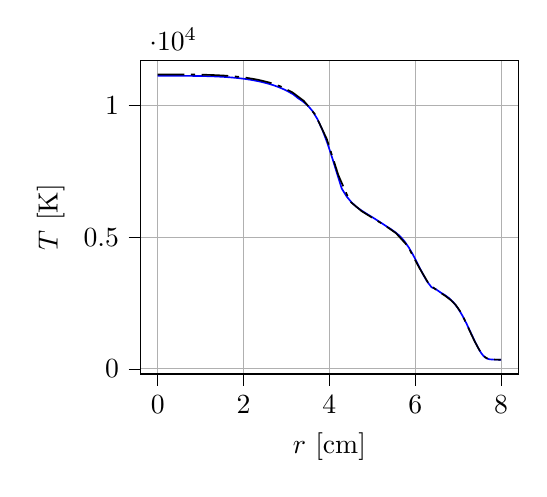
\begin{tikzpicture}

\definecolor{darkgray176}{RGB}{176,176,176}

\begin{axis}[
legend cell align=left,
legend pos= north east,
scale = .7,
ylabel = {$T$ [K]},
tick align=outside,
tick pos=left,
xlabel = {$r$ [cm]},
x grid style={darkgray176},
xmajorgrids,
xmin=-0.399999991059303, xmax=8.39999981224537,
xtick style={color=black},
y grid style={darkgray176},
ymajorgrids,
ymin=-191.189754927365, ymax=11714.9854159589,
ytick style={color=black}
]
\addplot [semithick, blue]
table {%
0 11120.774489647
0.007999999797903 11120.7741022209
0.015999999595806 11120.7737147958
0.023999999393709 11120.7733273718
0.031999999191612 11120.7729399487
0.039999998989515 11120.7725525268
0.047999998787418 11120.7721651058
0.0560000014957041 11120.7717776857
0.063999998383224 11120.771390267
0.0720000010915101 11120.7710028489
0.07999999797903 11120.7706154322
0.0880000006873161 11120.7702280163
0.095999997574836 11120.7698406016
0.104000000283122 11120.7689970492
0.112000002991408 11120.7672231838
0.119999994058162 11120.7654493241
0.127999996766448 11120.763675465
0.135999999474734 11120.7619016089
0.14400000218302 11120.7601277559
0.151999993249774 11120.7583539086
0.15999999595806 11120.7565800618
0.167999998666346 11120.7548062181
0.176000001374632 11120.7530323774
0.183999992441386 11120.7512585425
0.191999995149672 11120.7494847081
0.199999986216426 11120.7477108793
0.208000000566244 11120.7433486099
0.215999991632998 11120.7376409674
0.224000005982816 11120.7319333136
0.23199999704957 11120.7262256817
0.239999988116324 11120.7205180551
0.248000002466142 11120.7148104172
0.255999993532896 11120.7091028012
0.26399998459965 11120.7033951905
0.271999998949468 11120.6976875685
0.279999990016222 11120.6919799684
0.28800000436604 11120.686272357
0.295999995432794 11120.6805647676
0.303999986499548 11120.6748571834
0.312000000849366 11120.6614492091
0.31999999191612 11120.6479397898
0.327999982982874 11120.6344303782
0.335999997332692 11120.620920935
0.343999988399446 11120.607411539
0.352000002749264 11120.5939021113
0.359999993816018 11120.5803927307
0.367999984882772 11120.5668833578
0.37599999923259 11120.5533739534
0.383999990299344 11120.539864596
0.392000004649162 11120.5263552071
0.399999972432852 11120.5128459045
0.40799998678267 11120.4952316509
0.416000001132488 11120.4687317178
0.423999968916178 11120.4422319495
0.431999983265996 11120.4157320374
0.439999997615814 11120.3892321359
0.448000011965632 11120.3627322448
0.455999979749322 11120.3362325185
0.46399999409914 11120.3097326484
0.472000008448958 11120.2832327888
0.479999976232648 11120.2567330939
0.487999990582466 11120.2302332553
0.496000004932284 11120.2037334272
0.503999972715974 11120.1772337639
0.511999987065792 11120.1381567215
0.52000000141561 11120.0921570072
0.5279999691993 11120.0461575743
0.535999983549118 11120.0001578872
0.543999997898936 11119.9541582137
0.551999965682626 11119.9081588216
0.559999980032444 11119.8621591753
0.567999994382262 11119.8161595426
0.57600000873208 11119.7701599235
0.58399997651577 11119.7241605858
0.591999990865588 11119.6781609939
0.600000005215406 11119.6321614156
0.607999972999096 11119.5861621187
0.615999987348914 11119.5135435367
0.624000001698732 11119.4402140733
0.631999969482422 11119.366885054
0.63999998383224 11119.293555625
0.647999998182058 11119.2202262132
0.655999965965748 11119.1468972454
0.663999980315566 11119.073567868
0.671999994665384 11119.0002385077
0.679999962449074 11118.9269095914
0.687999976798892 11118.8535802655
0.69599999114871 11118.7802509568
0.704000005498528 11118.7069216652
0.711999973282218 11118.6225396316
0.719999987632036 11118.5127297824
0.728000001981854 11118.4029199544
0.735999969765544 11118.293110787
0.743999984115362 11118.1833010016
0.75199999846518 11118.0734912375
0.75999996624887 11117.9636821338
0.767999980598688 11117.8538724122
0.775999994948506 11117.744062712
0.784000009298325 11117.634253033
0.791999977082014 11117.5244440145
0.799999944865704 11117.4146350172
0.808000005781651 11117.3048247629
0.81599997356534 11117.1653427276
0.82399994134903 11117.0085821459
0.832000002264977 11116.8518197653
0.839999970048666 11116.6950592357
0.847999937832355 11116.538298732
0.855999998748302 11116.3815364294
0.863999966531992 11116.2247759777
0.871999934315681 11116.068015552
0.879999995231628 11115.9112533273
0.887999963015318 11115.7544929536
0.896000023931265 11115.5977307809
0.903999991714954 11115.4409704592
0.911999959498644 11115.2842101635
0.920000020414591 11115.0709954118
0.92799998819828 11114.8554916552
0.93599995598197 11114.6399879301
0.944000016897917 11114.4244817276
0.951999984681606 11114.2089780653
0.959999952465296 11113.9934744344
0.968000013381243 11113.7779683262
0.975999981164932 11113.5624647581
0.983999948948622 11113.3469612215
0.992000009864569 11113.1314552075
0.999999977648258 11112.9159517337
1.00799994543195 11112.7004482914
1.01600000634789 11112.4652262003
1.02399997413158 11112.1788621652
1.03199994191527 11111.8924982973
1.04000000283122 11111.6061312628
1.04799997061491 11111.3197677291
1.0559999383986 11111.0334043624
1.06399999931455 11110.747037829
1.07199996709824 11110.4606747963
1.07999993488193 11110.1743119306
1.08799999579787 11109.887945898
1.09599996358156 11109.6015833661
1.10399993136525 11109.315221001
1.1119999922812 11109.028855469
1.11999996006489 11108.7203702449
1.12800002098083 11108.346540597
1.13599998876452 11107.9727155069
1.14399995654821 11107.5988906228
1.15200001746416 11107.2250615927
1.15999998524785 11106.8512371204
1.16799995303154 11106.4774128539
1.17600001394749 11106.1035844413
1.18399998173118 11105.7297605864
1.19199994951487 11105.3559369372
1.20000001043081 11104.9821091417
1.2079999782145 11104.6082859038
1.21599994599819 11104.2344628715
1.22400000691414 11103.8386929187
1.23199997469783 11103.3632418033
1.23999994248152 11102.8877909389
1.24800000339746 11102.4123347905
1.25599997118115 11101.9368844279
1.26399993896484 11101.4614343161
1.27199999988079 11100.9859789201
1.27999996766448 11100.5105293099
1.28799993544817 11100.0350799503
1.29599999636412 11099.5596253065
1.30399996414781 11099.0841764482
1.3119999319315 11098.6087278404
1.31999999284744 11098.1332739482
1.32799996063113 11097.6368437743
1.33599992841482 11097.0441024284
1.34399998933077 11096.451354485
1.35199995711446 11095.8586137449
1.35999992489815 11095.2658733078
1.36799998581409 11094.673126273
1.37599995359778 11094.0803864415
1.38400001451373 11093.4876400122
1.39199998229742 11092.894900786
1.39999995008111 11092.3021618624
1.40800001099706 11091.7094163409
1.41599997878075 11091.1166780224
1.42399994656444 11090.5239400063
1.43200000748038 11089.9121176247
1.43999997526407 11089.1849218776
1.44799994304776 11088.4577264933
1.45600000396371 11087.7305230062
1.4639999717474 11087.0033283476
1.47199993953109 11086.2761340516
1.48000000044703 11085.5489316527
1.48799996823072 11084.8217380819
1.49599993601441 11084.0945448736
1.50399999693036 11083.3673435622
1.51199996471405 11082.6401510788
1.51999993249774 11081.9129589576
1.52799999341369 11081.1857587331
1.53599996119738 11080.4425062615
1.54399992898107 11079.5621919391
1.55199998989701 11078.6818678
1.5599999576807 11077.8015543407
1.56800001859665 11076.9212310646
1.57599989324808 11076.0409287162
1.58399995416403 11075.1606063028
1.59200001507998 11074.2802843205
1.59999988973141 11073.3999832657
1.60799995064735 11072.5196621455
1.6160000115633 11071.6393414563
1.62399988621473 11070.7590416944
1.63199994713068 11069.8787218669
1.64000000804663 11068.9866323977
1.64799988269806 11067.9330480202
1.65599994361401 11066.8794396217
1.66400000452995 11065.8258317329
1.67199987918139 11064.7722488848
1.67999994009733 11063.7186420153
1.68800000101328 11062.6650356555
1.69599987566471 11061.611454336
1.70399993658066 11060.5578489948
1.7119999974966 11059.5042441629
1.71999987214804 11058.4506643712
1.72799993306398 11057.3970605575
1.73599999397993 11056.3434572528
1.74399986863136 11055.283845868
1.75199992954731 11054.0352888031
1.75999999046326 11052.7867323368
1.7680000513792 11051.5381764689
1.77599992603064 11050.2896502693
1.78399998694658 11049.041095598
1.79200004786253 11047.7925415249
1.79999992251396 11046.5440171196
1.80799998342991 11045.2954642423
1.81600004434586 11044.046911963
1.82399991899729 11042.7983893511
1.83199997991323 11041.549838267
1.84000004082918 11040.3012877803
1.84799991548061 11039.0527669608
1.85599997639656 11037.5874047132
1.86400003731251 11036.1207366449
1.87199991196394 11034.6541034236
1.87999997287989 11033.1874367526
1.88800003379583 11031.7207707799
1.89599990844727 11030.2541396539
1.90399996936321 11028.7874750778
1.91200003027916 11027.3208111997
1.91999990493059 11025.8541821679
1.92799996584654 11024.3875196856
1.93600002676249 11022.920857901
1.94399990141392 11021.454230962
1.95199996232986 11019.9875705723
1.96000002324581 11018.2885448305
1.96799989789724 11016.5791417014
1.97599995881319 11014.8696995825
1.98400001972914 11013.1602582744
1.99199989438057 11011.4508575777
1.99999995529652 11009.741417891
2.00800001621246 11008.0319790145
2.0159998908639 11006.3225807489
2.02399995177984 11004.613143493
2.03200001269579 11002.9037070469
2.03999988734722 11001.1943112112
2.04799994826317 10999.4848763845
2.05600000917912 10997.7754423674
2.06399988383055 10995.7649476285
2.07199994474649 10993.7842299096
2.08000000566244 10991.8035099539
2.08799988031387 10989.8228338801
2.09599994122982 10987.8421094564
2.10400000214577 10985.8613828014
2.1119998767972 10983.8807000344
2.11999993771315 10981.8999689229
2.12799999862909 10979.9192355859
2.13599987328053 10977.9385461427
2.14399993419647 10975.9578083606
2.15199999511242 10973.9770683587
2.15999986976385 10971.9963722564
2.1679999306798 10969.9174291845
2.17599999159575 10967.597195405
2.18399986624718 10965.2770127397
2.19199992716312 10962.9567731476
2.19999998807907 10960.6365306528
2.2079998627305 10958.3163392799
2.21599992364645 10955.9960909869
2.2239999845624 10953.6758397992
2.23199985921383 10951.3556397413
2.23999992012978 10949.0353827705
2.24799998104572 10946.7151229119
2.25600004196167 10944.3948601679
2.2639999166131 10942.0746485635
2.27199997752905 10939.7543800561
2.280000038445 10937.194158609
2.28799991309643 10934.5094231133
2.29599997401237 10931.8246216308
2.30400003492832 10929.1398166742
2.31199990957975 10926.4550707566
2.3199999704957 10923.7702588609
2.32800003141165 10921.0854434998
2.33599990606308 10918.400687187
2.34399996697903 10915.7158649045
2.35200002789497 10913.0310391656
2.35999990254641 10910.3462724839
2.36799996346235 10907.661439841
2.3760000243783 10904.9766037505
2.38399989902973 10902.2807719726
2.39199995994568 10899.1886340954
2.40000002086163 10896.0964921414
2.40799989551306 10893.0044181082
2.415999956429 10889.9122680112
2.42400001734495 10886.8201138477
2.43199989199638 10883.7280276157
2.43999995291233 10880.6358653297
2.44800001382828 10877.5436989878
2.45599988847971 10874.4516005878
2.46399994939566 10871.3594261439
2.4720000103116 10868.2672476541
2.47999988496304 10865.1751371169
2.48799994587898 10862.0829505458
2.49600000679493 10858.8055293161
2.50399988144636 10855.2456145415
2.51199994236231 10851.6856120602
2.52000000327826 10848.125604763
2.52799987792969 10844.5656755416
2.53599993884563 10841.0056586252
2.54399999976158 10837.4456369047
2.55199987441301 10833.8856932725
2.55999993532896 10830.3256619583
2.56799999624491 10826.7656258517
2.57599987089634 10823.2056678458
2.58399993181229 10819.6456221684
2.59199999272823 10816.0855717116
2.59999986737967 10812.5255993678
2.60799992829561 10808.5479957926
2.61599998921156 10804.441879384
2.62399986386299 10800.33585275
2.63199992477894 10796.2297246908
2.63999998569489 10792.1235908137
2.64799986034632 10788.0175467263
2.65599992126226 10783.9114012279
2.66399998217821 10779.8052499262
2.67199985682964 10775.6991884293
2.67999991774559 10771.5930255355
2.68799997866154 10767.486856853
2.69599985331297 10763.3807779902
2.70399991422892 10759.2745977447
2.71199997514486 10755.0828304837
2.7199998497963 10750.3347086993
2.72799991071224 10745.5864691453
2.73599997162819 10740.8382223803
2.74399984627962 10736.0900789634
2.75199990719557 10731.3418177946
2.75999996811152 10726.5935494314
2.76800002902746 10721.8452738837
2.77599990367889 10717.0971017081
2.78399996459484 10712.3488118035
2.79200002551079 10707.6005147299
2.79999990016222 10702.8523210477
2.80799996107817 10698.1040096542
2.81600002199411 10693.3556911096
2.82399989664555 10688.2282144426
2.83199995756149 10682.7241062551
2.84000001847744 10677.2199889793
2.84799989312887 10671.7159907746
2.85599995404482 10666.2118553448
2.86400001496077 10660.7077108493
2.8719998896122 10655.2036854479
2.87999995052814 10649.6995228424
2.88800001144409 10644.1953511967
2.89599988609552 10638.691298667
2.90399994701147 10633.1871089562
2.91200000792742 10627.6829102247
2.91999988257885 10622.178830634
2.9279999434948 10616.6746138839
2.93600000441074 10610.3982312733
2.94399987906218 10604.0068900967
2.95199993997812 10597.6153885594
2.96000000089407 10591.2238754833
2.9679998755455 10584.8324996912
2.97599993646145 10578.4409635664
2.9839999973774 10572.0494159314
2.99199987202883 10565.6580056099
2.99999993294477 10559.2664349834
3.00799999386072 10552.8748528753
3.01599986851215 10546.4834081101
3.0239999294281 10540.0918030676
3.03199999034405 10533.700186572
3.03999986499548 10527.0613759106
3.04799992591143 10519.6332542105
3.05599998682737 10512.2051177959
3.06399986147881 10504.7771396279
3.07199992239475 10497.348973821
3.0799999833107 10489.920793336
3.08799985796213 10482.4927711334
3.09599991887808 10475.0645613296
3.10399997979403 10467.6363368841
3.11199985444546 10460.2082707591
3.1199999153614 10452.7800170658
3.12799997627735 10445.3517487669
3.1360000371933 10437.9234658745
3.14400009810925 10430.4951684005
3.15199978649616 10428.8076966284
3.15999984741211 10418.1665912233
3.16799990832806 10407.525489183
3.175999969244 10396.8843904969
3.18400003015995 10386.2432951543
3.1920000910759 10375.602203145
3.19999977946281 10364.9616099688
3.20799984037876 10354.3205245942
3.21599990129471 10343.6794425216
3.22399996221066 10333.0383637407
3.2320000231266 10322.397288241
3.24000008404255 10311.7562160125
3.24799977242947 10301.1156425544
3.25599983334541 10290.4745768373
3.26399989426136 10280.3724419342
3.27199995517731 10271.5355776639
3.28000001609325 10262.6987150538
3.2880000770092 10253.8618540986
3.29599976539612 10245.0254062885
3.30399982631207 10236.188548628
3.31199988722801 10227.3516926071
3.31999994814396 10218.5148382204
3.32800000905991 10209.6779854642
3.33600006997585 10200.8411343321
3.34399975836277 10192.0046963143
3.35199981927872 10183.1678484163
3.35999988019466 10174.331002128
3.36799994111061 10165.4941574443
3.37600000202656 10156.6573143604
3.3840000629425 10146.0134503313
3.39199975132942 10135.3527654317
3.39999981224537 10124.6915871868
3.40799987316132 10114.0304120334
3.41599993407726 10103.3692399621
3.42399999499321 10092.7080709634
3.43200005590916 10082.0469050274
3.43999974429607 10071.3862385921
3.44799980521202 10060.7250787554
3.45599986612797 10050.0639219542
3.46399992704391 10039.4027681793
3.47199998795986 10028.7416174216
3.48000004887581 10018.0804696719
3.48799973726273 10007.4198213656
3.49599979817867 9993.71446507112
3.50399985909462 9978.59122304875
3.51199992001057 9963.46798706366
3.51999998092651 9948.34475709769
3.52800004184246 9933.22153313273
3.53600010275841 9918.09831515077
3.54399979114532 9902.9758073578
3.55199985206127 9887.85260128779
3.55999991297722 9872.72940114713
3.56799997389317 9857.60620691811
3.57600003480911 9842.48301858305
3.58400009572506 9827.35983612435
3.59199978411198 9812.23736374679
3.59999984502792 9797.11419298805
3.60799990594387 9779.70624287424
3.61599996685982 9758.47396075342
3.62400002777576 9737.24168765491
3.63200008869171 9716.00942355193
3.63999977707863 9694.77815711402
3.64799983799458 9673.54591092181
3.65599989891052 9652.31367364544
3.66399995982647 9631.08144525857
3.67200002074242 9609.84922573496
3.68000008165836 9588.61701504843
3.68799977004528 9567.38580186668
3.69599983096123 9546.15360877593
3.70399989187717 9524.92142444444
3.71199995279312 9503.6892488465
3.72000001370907 9482.01235520918
3.72800007462502 9454.01476665823
3.73599976301193 9426.01849260124
3.74399982392788 9398.02092554892
3.75199988484383 9370.02336919903
3.75999994575977 9342.02582352029
3.76800000667572 9314.02828848158
3.77600006759167 9286.03076405136
3.78399975597858 9258.0345539259
3.79199981689453 9230.03705062109
3.79999987781048 9202.03955783294
3.80799993872643 9174.0420755309
3.81599999964237 9146.04460368454
3.82400006055832 9118.04714226355
3.83199974894524 9090.05099496049
3.83999980986118 9057.1826082153
3.84799987077713 9022.75412533453
3.85599993169308 8988.32565259085
3.86399999260902 8953.89718995501
3.87200005352497 8919.46873739789
3.87999974191189 8885.0418980773
3.88799980282784 8850.6134655902
3.89599986374378 8816.18504309508
3.90399992465973 8781.75663056327
3.91199998557568 8747.32822796619
3.92000004649162 8712.89983527537
3.92799973487854 8678.47305564653
3.93599979579449 8644.0446826828
3.94399985671043 8609.61631954059
3.95199991762638 8572.89477525304
3.95999997854233 8533.36040858478
3.96800003945827 8493.82604812291
3.97599972784519 8454.29353479743
3.98399978876114 8414.75918669511
3.99199984967709 8375.22484474638
3.99999991059303 8335.69050893378
4.00799997150898 8296.1561792399
4.01600003242493 8256.62185564741
4.02400009334087 8217.08753813905
4.03199978172779 8177.55506764327
4.03999984264374 8138.02076225133
4.04799990355968 8098.48646289208
4.05599996447563 8058.95216954853
4.06400002539158 8019.02498888003
4.07200008630753 7976.7003574735
4.07999977469444 7934.37769504735
4.08799983561039 7892.0530598483
4.09599989652634 7849.72842276092
4.10399995744228 7807.40378379052
4.11200001835823 7765.07914294236
4.12000007927418 7722.75450022168
4.12799976766109 7680.43182651366
4.13599982857704 7638.10718006377
4.14399988949299 7595.78253175704
4.15199995040894 7553.45788159863
4.16000001132488 7511.1332295937
4.16800007224083 7468.8085757474
4.17599976062775 7426.48589094523
4.18399982154369 7384.59070204213
4.19199988245964 7342.7819520111
4.19999994337559 7300.97318709448
4.20800000429153 7259.1644073335
4.21600006520748 7217.35561276924
4.2239997535944 7175.54875030256
4.23199981451035 7133.73992625509
4.23999987542629 7091.93108752668
4.24799993634224 7050.12223415782
4.25599999725819 7008.31336618885
4.26400005817413 6966.50448365995
4.27199974656105 6924.69753347514
4.279999807477 6882.88862194702
4.28799986839294 6841.07969597863
4.29599992930889 6822.2376158723
4.30399999022484 6801.21079412412
4.31200005114079 6780.18401937923
4.3199997395277 6759.15827089202
4.32799980044365 6738.13159054092
4.3359998613596 6717.10495758349
4.34399992227554 6696.07837215081
4.35199998319149 6675.05183437446
4.36000004410744 6654.02534438651
4.36799973249435 6632.99988143092
4.3759997934103 6611.97348741564
4.38399985432625 6590.94714158787
4.3919999152422 6569.92084408162
4.39999997615814 6548.89459503144
4.40800003707409 6529.81702886024
4.41599972546101 6514.29947147715
4.42399978637695 6498.78121659099
4.4319998472929 6483.26298689325
4.43999990820885 6467.74478245436
4.44799996912479 6452.22660334506
4.45600003004074 6436.70844963631
4.46399971842766 6421.19104401241
4.47199977934361 6405.67294131758
4.47999984025955 6390.15486423783
4.4879999011755 6374.63681284521
4.49599996209145 6359.11878721203
4.50400002300739 6343.6007874109
4.51200008392334 6328.08281351466
4.51999977231026 6313.25245789295
4.5279998332262 6301.4769364025
4.53599989414215 6289.70142584603
4.5439999550581 6277.92592625448
4.55200001597404 6266.15043765894
4.56000007688999 6254.37496009059
4.56799976527691 6242.60004191421
4.57599982619286 6230.82458649425
4.5839998871088 6219.04914219485
4.59199994802475 6207.27370904905
4.6000000089407 6195.49828708819
4.60800006985664 6183.72287634418
4.61599975824356 6171.94802517938
4.62399981915951 6160.17263696475
4.63199988007545 6148.39726006342
4.6399999409914 6138.948820922
4.64800000190735 6129.46955849167
4.6560000628233 6119.99029926759
4.66399975121021 6110.5114846678
4.67199981212616 6101.03223188374
4.67999987304211 6091.55298233368
4.68799993395805 6082.07373602712
4.695999994874 6072.5944929728
4.70400005578995 6063.11525318073
4.71199974417686 6053.63645806802
4.71999980509281 6044.15722482818
4.72799986600876 6034.67799487875
4.73599992692471 6025.19876822927
4.74399998784065 6015.71954488931
4.7520000487566 6007.22622119085
4.75999973714352 5998.91632474972
4.76799979805946 5990.60604182017
4.77599985897541 5982.29575937842
4.78399991989136 5973.98547742589
4.7919999808073 5965.67519596401
4.80000004172325 5957.3649149942
4.80799973011017 5949.05502149255
4.81599979102612 5940.74474151119
4.82399985194206 5932.43446202625
4.83199991285801 5924.12418303917
4.83999997377396 5915.81390455142
4.8480000346899 5907.50362656446
4.85599972307682 5899.19373605425
4.86399978399277 5891.12649201671
4.87199984490871 5883.17708922817
4.87999990582466 5875.22768762964
4.88799996674061 5867.27828722464
4.89600002765656 5859.32888801668
4.90399971604347 5851.37986017917
4.91199977695942 5843.43046337589
4.91999983787537 5835.48106778033
4.92799989879131 5827.53167339607
4.93599995970726 5819.58228022669
4.94400002062321 5811.63288827581
4.95199970901012 5803.68386771657
4.95999976992607 5795.73447821352
4.96799983084202 5787.78508993989
4.97599989175797 5779.77117100462
4.98399995267391 5771.6936602146
4.99200001358986 5763.61615291532
4.99999970197678 5755.53902525236
5.00799976289272 5747.46152496577
5.01599982380867 5739.38402820138
5.02399988472462 5731.30653496976
5.03199994564056 5723.22904528154
5.04000000655651 5715.15155914735
5.04800006747246 5707.07407657791
5.05599975585938 5698.99697371793
5.06399981677532 5690.91949831008
5.07199987769127 5682.84202649933
5.07999993860722 5674.76455829655
5.08799999952316 5666.58753662509
5.09600006043911 5658.21197318629
5.10399974882603 5649.8368050867
5.11199980974197 5641.46125231376
5.11999987065792 5633.08570489819
5.12799993157387 5624.71016285627
5.13599999248981 5616.33462620436
5.14400005340576 5607.9590949589
5.15199974179268 5599.58395914907
5.15999980270863 5591.20843876576
5.16799986362457 5582.83292383856
5.17599992454052 5574.45741438417
5.18399998545647 5566.08191041935
5.19200004637241 5557.70641196092
5.19999973475933 5549.30680448618
5.20799979567528 5540.78221635172
5.21599985659122 5532.25763258211
5.22399991750717 5523.7330531908
5.23199997842312 5515.20847819128
5.24000003933907 5506.6839075971
5.24799972772598 5498.15973837477
5.25599978864193 5489.63517663218
5.26399984955788 5481.11061933538
5.27199991047382 5472.58606649894
5.27999997138977 5464.06151813641
5.28800003230572 5455.53697426168
5.29599972069263 5447.01283184038
5.30399978160858 5438.48829698295
5.31199984252453 5429.96376665533
5.31999990344048 5421.756451072
5.32799996435642 5413.55075948802
5.33600002527237 5405.34506588376
5.34399971365929 5397.13975235752
5.35199977457523 5388.93405469382
5.35999983549118 5380.7283549908
5.36799989640713 5372.52265324241
5.37599995732307 5364.31694944123
5.38400001823902 5356.1112435818
5.39199970662594 5347.9059177625
5.39999976754189 5339.70020776654
5.40799982845783 5331.49449569249
5.41599988937378 5323.28878153379
5.42399995028973 5315.08306528385
5.43200001120567 5304.39231420068
5.43999969959259 5295.45288148643
5.44799976050854 5286.51303212278
5.45599982142448 5277.57318240039
5.46399988234043 5268.63333231896
5.47199994325638 5259.69348187815
5.48000000417233 5250.7536310778
5.48799969255924 5241.81419620827
5.49599975347519 5232.87434468747
5.50399981439114 5223.93449280603
5.51199987530708 5214.99464056363
5.51999993622303 5206.05478795996
5.52799999713898 5197.11493499468
5.53600005805492 5187.03629198195
5.54399974644184 5176.10352537874
5.55199980735779 5165.1702479041
5.55999986827374 5154.23696867287
5.56799992918968 5143.30368768351
5.57599999010563 5132.37040493444
5.58400005102158 5121.43712042413
5.59199973940849 5110.50434326795
5.59999980032444 5099.57105523049
5.60799986124039 5088.63776542709
5.61599992215633 5077.70447385617
5.62399998307228 5066.77118051615
5.63200004398823 5055.83788540548
5.63999973237514 5043.77966224354
5.64799979329109 5029.29532359747
5.65599985420704 5014.81098259091
5.66399991512299 5000.32663922175
5.67199997603893 4985.84229348791
5.68000003695488 4971.35794538727
5.6879997253418 4956.87426939332
5.69599978625774 4942.38991655503
5.70399984717369 4927.90556133876
5.71199990808964 4913.42120374995
5.71999996900558 4898.93684378379
5.72800002992153 4884.45248143815
5.73599971830845 4869.96879118662
5.7439997792244 4855.22215482303
5.75199984014034 4836.55090840121
5.75999990105629 4817.87965964821
5.76799996197224 4799.20840856197
5.77600002288818 4780.5371551404
5.7839997112751 4761.86676882294
5.79199977219105 4743.19551072691
5.79999983310699 4724.52425028597
5.80799989402294 4705.85298750088
5.81599995493889 4687.18172237141
5.82400001585484 4668.51045489406
5.83199970424175 4649.8400545089
5.8399997651577 4631.16878232957
5.84799982607365 4612.49750779604
5.85599988698959 4590.6728824377
5.86399994790554 4568.10067014743
5.87200000882149 4545.52845602673
5.8799996972084 4522.95729116671
5.88799975812435 4500.3850733803
5.8959998190403 4477.81285375854
5.90399987995625 4455.24063230006
5.91199994087219 4432.66840900233
5.92000000178814 4410.09618386459
5.92799969017506 4387.52500797816
5.935999751091 4364.95277915493
5.94399981200695 4342.38054848642
5.9519998729229 4319.80831597099
5.95999993383884 4295.74382411039
5.96799999475479 4270.47838362241
5.97599968314171 4245.21411861786
5.98399974405766 4219.94867608611
5.9919998049736 4194.68323253107
5.99999986588955 4169.41778795182
6.0079999268055 4144.15234234748
6.01599998772144 4118.88689571698
6.02400004863739 4093.62144805954
6.03199973702431 4068.35717587939
6.03999979794025 4043.09172616526
6.0479998588562 4017.82627542135
6.05599991977215 3992.56082364675
6.0639999806881 3967.12636338291
6.07200004160404 3941.29720152034
6.07999972999096 3915.46924233402
6.08799979090691 3889.64008031404
6.09599985182285 3863.81091821524
6.1039999127388 3837.98175603757
6.11199997365475 3812.15259378206
6.12000003457069 3786.32343145005
6.12799972295761 3760.49547178547
6.13599978387356 3734.66630929155
6.14399984478951 3708.83714671839
6.15199990570545 3683.00798406592
6.1599999666214 3657.17882133406
6.16800002753735 3631.46297513346
6.17599971592426 3608.12246996673
6.18399977684021 3584.78087869989
6.19199983775616 3561.43928825303
6.1999998986721 3538.09769862688
6.20799995958805 3514.75610982219
6.216000020504 3491.41452184294
6.22399970889091 3468.07402160089
6.23199976980686 3444.73243526333
6.23999983072281 3421.39084975189
6.24799989163876 3398.04926506565
6.2559999525547 3374.70768120536
6.26399964094162 3351.36718509062
6.2720000743866 3328.02451596561
6.27999976277351 3309.79599605125
6.28800019621849 3292.91424170255
6.29599988460541 3276.03406099405
6.30399957299232 3259.15388177633
6.3120000064373 3242.27213190052
6.31999969482422 3225.39195566856
6.3280001282692 3208.51020878171
6.33599981665611 3191.63003554078
6.34399950504303 3174.74986379763
6.35199993848801 3157.8681214039
6.35999962687492 3140.98795266016
6.3680000603199 3124.10621326886
6.37599974870682 3107.22604753002
6.38400018215179 3096.44278441437
6.39199987053871 3090.91752076917
6.39999955892563 3085.39225886338
6.40799999237061 3079.86648409865
6.41599968075752 3074.34122567659
6.4240001142025 3068.81545439912
6.43199980258942 3063.29019946719
6.43999949097633 3057.7649462826
6.44799992442131 3052.2391802479
6.45599961280823 3046.71393056304
6.4640000462532 3041.18816803159
6.47199973464012 3035.66292185286
6.4800001680851 3030.13716283108
6.48799985647202 3017.13551660439
6.49599954485893 3008.01980328442
6.50399997830391 2998.90323979455
6.51199966669083 2989.78752413542
6.5200001001358 2980.67095830502
6.52799978852272 2971.55524030483
6.5360002219677 2962.43867213374
6.54399991035461 2953.32295179272
6.55199959874153 2944.20723028109
6.56000003218651 2935.09065859771
6.56799972057343 2925.97493474337
6.5760001540184 2916.8583607171
6.58399984240532 2907.74263452048
6.59199953079224 2899.35439807189
6.59999996423721 2891.44162585298
6.60799965262413 2883.52958533851
6.61600008606911 2875.61680273828
6.62399977445602 2867.70475184135
6.632000207901 2859.79195885592
6.63999989628792 2851.87989757393
6.64799958467484 2843.9678310985
6.65600001811981 2836.05502253085
6.66399970650673 2828.1429456658
6.67200013995171 2820.23012670517
6.67999982833862 2812.31803944702
6.68799951672554 2804.40594699155
6.69599995017052 2795.14519254034
6.70399963855743 2785.77759822138
6.71200007200241 2776.40912395659
6.71999976038933 2767.04151466299
6.7280001938343 2757.67302541944
6.73599988222122 2748.30540114739
6.74399957060814 2738.93776938482
6.75200000405312 2729.56925766691
6.75999969244003 2720.20161091933
6.76800012588501 2710.83308421283
6.77599981427193 2701.46542247466
6.78399950265884 2692.09775324112
6.79199993610382 2681.9137826691
6.79999962449074 2669.25458984644
6.80800005793571 2656.59420987042
6.81599974632263 2643.93500079234
6.82400017976761 2631.27460455589
6.83199986815453 2618.61537921595
6.83999955654144 2605.9561457443
6.84799998998642 2593.29572510972
6.85599967837334 2580.63647537036
6.86400011181831 2567.97603846417
6.87199980020523 2555.31677245118
6.87999948859215 2542.65749830103
6.88799992203712 2529.99703697807
6.89599961042404 2514.88685599192
6.90400004386902 2497.92162166401
6.91199973225594 2480.95796007256
6.92000016570091 2463.99271136605
6.92799985408783 2447.02903539401
6.93599954247475 2430.06535223085
6.94399997591972 2413.10008194689
6.95199966430664 2396.1363843977
6.96000009775162 2379.17109972426
6.96799978613853 2362.20738778483
6.97599947452545 2345.24366864721
6.98399990797043 2328.27836238104
6.99199959635735 2311.31462884752
7.00000002980232 2290.34434058004
7.00799971818924 2268.88655512193
7.01600015163422 2247.42676643646
7.02399984002113 2225.96897149968
7.03199952840805 2204.51117182339
7.03999996185303 2183.05136891506
7.04799965023994 2161.59355975721
7.05600008368492 2140.13374736504
7.06399977207184 2118.67592872286
7.07200020551682 2097.21610684409
7.07999989390373 2075.75827871215
7.08799958229065 2054.30044583719
7.09600001573563 2032.01878926647
7.10399970412254 2006.70039444465
7.11200013756752 1981.37964072054
7.11999982595444 1956.06124419792
7.12799951434135 1930.74284682173
7.13599994778633 1905.42209054297
7.14399963617325 1880.10369146436
7.15200006961823 1854.78293348276
7.15999975800514 1829.46453270123
7.16800019145012 1804.1437730163
7.17599987983704 1778.82537052909
7.18399956822395 1753.50696719096
7.19200000166893 1728.18620494852
7.19999969005585 1701.58267510324
7.20800012350082 1673.85779264926
7.21599981188774 1646.13549653858
7.22399950027466 1618.41320483195
7.23199993371964 1590.68833558709
7.23999962210655 1562.9660526866
7.24800005555153 1535.24119225237
7.25599974393845 1507.51891816296
7.26400017738342 1479.79406654193
7.27199986577034 1452.07180126618
7.27999955415726 1424.34954039515
7.28799998760223 1396.62470199701
7.29599967598915 1368.90244994453
7.30400010943413 1341.07136003811
7.31199979782104 1313.22505049192
7.31999948620796 1285.3787518955
7.32799991965294 1257.52987075734
7.33599960803986 1229.68359405967
7.34400004148483 1201.83473482881
7.35199972987175 1173.98848003959
7.36000016331673 1146.13964272244
7.36799985170364 1118.29340984809
7.37599954009056 1090.44718793309
7.38399997353554 1062.59838349468
7.39199966192245 1034.75218350255
7.40000009536743 1007.43425661406
7.40799978375435 982.567004221278
7.41599947214127 957.699770540943
7.42399990558624 932.830239548035
7.43199959397316 907.96304330176
7.44000002741814 883.093549750728
7.44799971580505 858.226390950863
7.45600014925003 833.356934855216
7.46399983763695 808.48981351274
7.47199952602386 783.6227109022
7.47999995946884 758.753311007208
7.48799964785576 733.886245869273
7.49600008130074 709.016883457715
7.50399976968765 686.147865077496
7.51200020313263 665.267490199258
7.51999989151955 644.914680313329
7.52799957990646 625.297732251368
7.53600001335144 606.144225943133
7.54399970173836 587.923021166014
7.55200013518333 570.075900825983
7.55999982357025 553.357661852225
7.56799951195717 536.903200550504
7.57599994540215 521.766739800742
7.58399963378906 506.767989244157
7.59200006723404 493.268114854939
7.59999975562096 479.769497671376
7.60800018906593 467.932376988456
7.61599987745285 456.096409450419
7.62399956583977 445.783786752098
7.63199999928474 435.608736787146
7.63999968767166 426.796370815081
7.64800012111664 418.255568834592
7.65599980950356 410.900049480306
7.66399949789047 403.939347832771
7.67199993133545 397.854303549209
7.67999961972237 392.208669023806
7.68800005316734 387.254318238747
7.69599974155426 382.794582391441
7.70400017499924 378.829296494642
7.71199986338615 375.359209422673
7.71999955177307 372.227653163065
7.72799998521805 369.569870956639
7.73599967360497 367.130522484154
7.74400010704994 365.127413720878
7.75199979543686 363.253438209905
7.75999948382378 361.766335492132
7.76799991726875 360.345122444824
7.77599960565567 359.254198906922
7.78400003910065 358.187817337721
7.79199972748756 357.392586333792
7.80000016093254 356.597281265318
7.80799984931946 356.01641021021
7.81599953770638 355.435534842834
7.82399997115135 354.994100140988
7.83199965953827 354.565395622122
7.84000009298325 354.229084163993
7.84799978137016 353.911315966445
7.85599946975708 353.644318848055
7.86399990320206 353.39422547814
7.87199959158897 353.173991286097
7.88000002503395 352.968657627575
7.88799971342087 352.778087718897
7.89600014686584 352.598033468834
7.90399983525276 352.42262693283
7.91199952363968 352.251851363635
7.91999995708466 352.079689232674
7.92799964547157 351.905624170534
7.93600007891655 351.727416985888
7.94399976730347 351.540975055223
7.95199945569038 351.350033963879
7.95999988913536 351.14557215152
7.96799957752228 350.937770134665
7.97600001096725 350.713145318321
7.98399969935417 350.486970619386
7.99200013279915 350.24348675594
7.99999982118607 350.000025567467
};
\addplot [semithick, black, dash pattern=on 9.6pt off 2.4pt on 1.5pt off 2.4pt]
table {%
0 11173.7956354641
0.00800800800800801 11173.7933480205
0.016016016016016 11173.7910605769
0.024024024024024 11173.7887731333
0.032032032032032 11173.7859213017
0.04004004004004 11173.7827540721
0.048048048048048 11173.7795868425
0.0560560560560561 11173.776419613
0.0640640640640641 11173.7732523834
0.0720720720720721 11173.7700851538
0.0800800800800801 11173.7669179242
0.0880880880880881 11173.7637506946
0.0960960960960961 11173.7605834651
0.104104104104104 11173.7574162355
0.112112112112112 11173.7542490059
0.12012012012012 11173.7510817763
0.128128128128128 11173.7479145467
0.136136136136136 11173.7447473172
0.144144144144144 11173.7415800876
0.152152152152152 11173.738412858
0.16016016016016 11173.7352456284
0.168168168168168 11173.7320783988
0.176176176176176 11173.7292485608
0.184184184184184 11173.7269611172
0.192192192192192 11173.7246736736
0.2002002002002 11173.7220711512
0.208208208208208 11173.7071799572
0.216216216216216 11173.6922887632
0.224224224224224 11173.6773975692
0.232232232232232 11173.6625063752
0.24024024024024 11173.6449246996
0.248248248248248 11173.627328978
0.256256256256256 11173.6097332564
0.264264264264264 11173.5921375348
0.272272272272272 11173.5745418132
0.28028028028028 11173.5569460916
0.288288288288288 11173.53935037
0.296296296296296 11173.5217546484
0.304304304304304 11173.5041589268
0.312312312312312 11173.4865632052
0.32032032032032 11173.4689674837
0.328328328328328 11173.4513717621
0.336336336336336 11173.4337760405
0.344344344344344 11173.4161803189
0.352352352352352 11173.3985845973
0.36036036036036 11173.3809888757
0.368368368368368 11173.3633931541
0.376376376376376 11173.3457974325
0.384384384384384 11173.3282017109
0.392392392392392 11173.3106059893
0.4004004004004 11173.2930102677
0.408408408408408 11173.2756449519
0.416416416416416 11173.2607537579
0.424424424424424 11173.2458625639
0.432432432432432 11173.2309713699
0.44044044044044 11173.2138146214
0.448448448448448 11173.15773175
0.456456456456456 11173.1016488787
0.464464464464464 11173.0455660073
0.472472472472473 11172.989483136
0.48048048048048 11172.9306602698
0.488488488488488 11172.8694631055
0.496496496496497 11172.8082659412
0.504504504504504 11172.747068777
0.512512512512513 11172.6858716127
0.520520520520521 11172.6246744484
0.528528528528528 11172.5634772842
0.536536536536537 11172.5022801199
0.544544544544545 11172.4410829556
0.552552552552553 11172.3798857914
0.560560560560561 11172.3186886271
0.568568568568569 11172.2574914628
0.576576576576577 11172.1962942986
0.584584584584585 11172.1350971343
0.592592592592593 11172.07389997
0.600600600600601 11172.0127028058
0.608608608608609 11171.9515056415
0.616616616616617 11171.8903084772
0.624624624624625 11171.829111313
0.632632632632633 11171.7679141487
0.640640640640641 11171.7067169844
0.648648648648649 11171.6455198202
0.656656656656657 11171.5843226559
0.664664664664665 11171.5231254916
0.672672672672673 11171.4619283274
0.680680680680681 11171.405678996
0.688688688688689 11171.3495961247
0.696696696696697 11171.2935132534
0.704704704704705 11171.237430382
0.712712712712713 11171.1374822336
0.720720720720721 11170.983530393
0.728728728728729 11170.8295785524
0.736736736736737 11170.6756267118
0.744744744744745 11170.5216748712
0.752752752752753 11170.3597867771
0.760760760760761 11170.1972917426
0.768768768768769 11170.0347967082
0.776776776776777 11169.8723016737
0.784784784784785 11169.7098066392
0.792792792792793 11169.5473116048
0.800800800800801 11169.3848165703
0.808808808808809 11169.2223215358
0.816816816816817 11169.0598265014
0.824824824824825 11168.8973314669
0.832832832832833 11168.7348364325
0.840840840840841 11168.572341398
0.848848848848849 11168.4098463635
0.856856856856857 11168.2473513291
0.864864864864865 11168.0848562946
0.872872872872873 11167.9223612601
0.880880880880881 11167.7598662257
0.888888888888889 11167.5973711912
0.896896896896897 11167.4348761567
0.904904904904905 11167.2723811223
0.912912912912913 11167.1098860878
0.920920920920921 11166.9473910534
0.928928928928929 11166.7848960189
0.936936936936937 11166.6224009844
0.944944944944945 11166.4629871028
0.952952952952953 11166.3090352622
0.960960960960961 11166.1550834216
0.968968968968969 11166.001131581
0.976976976976977 11165.8471797404
0.984984984984985 11165.5481657702
0.992992992992993 11165.2218098961
1.001001001001 11164.895454022
1.00900900900901 11164.569098148
1.01701701701702 11164.2385764026
1.02502502502503 11163.8992895016
1.03303303303303 11163.5600026005
1.04104104104104 11163.2207156995
1.04904904904905 11162.8814287984
1.05705705705706 11162.5421418974
1.06506506506507 11162.2028549963
1.07307307307307 11161.8635680953
1.08108108108108 11161.5242811942
1.08908908908909 11161.1849942932
1.0970970970971 11160.8457073921
1.10510510510511 11160.5064204911
1.11311311311311 11160.16713359
1.12112112112112 11159.827846689
1.12912912912913 11159.4885597879
1.13713713713714 11159.1492728869
1.14514514514515 11158.8099859858
1.15315315315315 11158.4706990847
1.16116116116116 11158.1314121837
1.16916916916917 11157.7921252826
1.17717717717718 11157.4528383816
1.18518518518519 11157.1135514805
1.19319319319319 11156.7742645795
1.2012012012012 11156.4349776784
1.20920920920921 11156.0956907774
1.21721721721722 11155.7661521213
1.22522522522523 11155.4397962473
1.23323323323323 11155.1134403732
1.24124124124124 11154.7870844991
1.24924924924925 11154.3985381706
1.25725725725726 11153.8071107728
1.26526526526527 11153.215683375
1.27327327327327 11152.6242559771
1.28128128128128 11152.0328285793
1.28928928928929 11151.4280971262
1.2972972972973 11150.8180722963
1.30530530530531 11150.2080474664
1.31331331331331 11149.5980226365
1.32132132132132 11148.9879978066
1.32932932932933 11148.3779729767
1.33733733733734 11147.7679481468
1.34534534534535 11147.157923317
1.35335335335335 11146.5478984871
1.36136136136136 11145.9378736572
1.36936936936937 11145.3278488273
1.37737737737738 11144.7178239974
1.38538538538539 11144.1077991675
1.39339339339339 11143.4977743376
1.4014014014014 11142.8877495077
1.40940940940941 11142.2777246779
1.41741741741742 11141.667699848
1.42542542542543 11141.0576750181
1.43343343343343 11140.4476501882
1.44144144144144 11139.8376253583
1.44944944944945 11139.2276005284
1.45745745745746 11138.6175756985
1.46546546546547 11138.0075508686
1.47347347347347 11137.3975260388
1.48148148148148 11136.7902364145
1.48948948948949 11136.1988090167
1.4974974974975 11135.6073816189
1.50550550550551 11135.0159542211
1.51351351351351 11134.4245268232
1.52152152152152 11133.5971626252
1.52952952952953 11132.6299363367
1.53753753753754 11131.6627100481
1.54554554554555 11130.6954837596
1.55355355355355 11129.725444631
1.56156156156156 11128.7323127008
1.56956956956957 11127.7391807706
1.57757757757758 11126.7460488404
1.58558558558559 11125.7529169101
1.59359359359359 11124.7597849799
1.6016016016016 11123.7666530497
1.60960960960961 11122.7735211195
1.61761761761762 11121.7803891893
1.62562562562563 11120.7872572591
1.63363363363363 11119.7941253288
1.64164164164164 11118.8009933986
1.64964964964965 11117.8078614684
1.65765765765766 11116.8147295382
1.66566566566567 11115.821597608
1.67367367367367 11114.8284656778
1.68168168168168 11113.8353337475
1.68968968968969 11112.8422018173
1.6976976976977 11111.8490698871
1.70570570570571 11110.8559379569
1.71371371371371 11109.8628060267
1.72172172172172 11108.8696740965
1.72972972972973 11107.8765421662
1.73773773773774 11106.883410236
1.74574574574575 11105.8902783058
1.75375375375375 11104.9111427801
1.76176176176176 11103.9439164915
1.76976976976977 11102.976690203
1.77777777777778 11102.0094639145
1.78578578578579 11101.0314848359
1.79379379379379 11099.5531202623
1.8018018018018 11098.0747556888
1.80980980980981 11096.5963911152
1.81781781781782 11095.1180265416
1.82582582582583 11093.621982258
1.83383383383383 11092.1083842804
1.84184184184184 11090.5947863029
1.84984984984985 11089.0811883253
1.85785785785786 11087.5675903477
1.86586586586587 11086.0539923702
1.87387387387387 11084.5403943926
1.88188188188188 11083.026796415
1.88988988988989 11081.5131984374
1.8978978978979 11079.9996004599
1.90590590590591 11078.4860024823
1.91391391391391 11076.9724045047
1.92192192192192 11075.4588065271
1.92992992992993 11073.9452085496
1.93793793793794 11072.431610572
1.94594594594595 11070.9180125944
1.95395395395395 11069.4044146169
1.96196196196196 11067.8908166393
1.96996996996997 11066.3772186617
1.97797797797798 11064.8636206841
1.98598598598599 11063.3500227066
1.99399399399399 11061.836424729
2.002002002002 11060.3228267514
2.01001001001001 11058.8092287739
2.01801801801802 11057.2956307963
2.02602602602603 11055.8149226242
2.03403403403403 11054.3365580507
2.04204204204204 11052.8581934771
2.05005005005005 11051.3798289035
2.05805805805806 11049.6168244989
2.06606606606607 11047.4513141072
2.07407407407407 11045.2858037155
2.08208208208208 11043.1202933238
2.09009009009009 11040.9547829321
2.0980980980981 11038.7468422174
2.10610610610611 11036.5339229196
2.11411411411411 11034.3210036218
2.12212212212212 11032.108084324
2.13013013013013 11029.8951650262
2.13813813813814 11027.6822457284
2.14614614614615 11025.4693264306
2.15415415415415 11023.2564071328
2.16216216216216 11021.043487835
2.17017017017017 11018.8305685372
2.17817817817818 11016.6176492394
2.18618618618619 11014.4047299416
2.19419419419419 11012.1918106438
2.2022022022022 11009.978891346
2.21021021021021 11007.7659720482
2.21821821821822 11005.5530527504
2.22622622622623 11003.3401334526
2.23423423423423 11001.1272141548
2.24224224224224 10998.914294857
2.25025025025025 10996.7013755592
2.25825825825826 10994.4884562614
2.26626626626627 10992.2755369636
2.27427427427427 10990.0626176657
2.28228228228228 10987.8496983679
2.29029029029029 10985.6522666896
2.2982982982983 10983.4867562979
2.30630630630631 10981.3212459062
2.31431431431431 10979.1557355145
2.32232232232232 10976.9902251228
2.33033033033033 10974.0691530267
2.33833833833834 10970.9678848659
2.34634634634635 10967.8666167051
2.35435435435435 10964.7653485443
2.36236236236236 10961.645665308
2.37037037037037 10958.4804975109
2.37837837837838 10955.3153297138
2.38638638638639 10952.1501619167
2.39439439439439 10948.9849941196
2.4024024024024 10945.8198263224
2.41041041041041 10942.6546585253
2.41841841841842 10939.4894907282
2.42642642642643 10936.3243229311
2.43443443443443 10933.159155134
2.44244244244244 10929.9939873369
2.45045045045045 10926.8288195397
2.45845845845846 10923.6636517426
2.46646646646647 10920.4984839455
2.47447447447447 10917.3333161484
2.48248248248248 10914.1681483513
2.49049049049049 10911.0029805542
2.4984984984985 10907.837812757
2.50650650650651 10904.6726449599
2.51451451451451 10901.5074771628
2.52252252252252 10898.3423093657
2.53053053053053 10895.1771415686
2.53853853853854 10892.0119737715
2.54654654654655 10888.8468059743
2.55455455455455 10885.6816381772
2.56256256256256 10882.5624717158
2.57057057057057 10879.461203555
2.57857857857858 10876.3599353942
2.58658658658659 10873.2586672334
2.59459459459459 10869.8928194612
2.6026026026026 10865.472966912
2.61061061061061 10861.0531143627
2.61861861861862 10856.6332618135
2.62662662662663 10852.2134092643
2.63463463463463 10847.7337390705
2.64264264264264 10843.2261008606
2.65065065065065 10838.7184626508
2.65865865865866 10834.2108244409
2.66666666666667 10829.7031862311
2.67467467467467 10825.1955480212
2.68268268268268 10820.6879098114
2.69069069069069 10816.1802716015
2.6986986986987 10811.6726333917
2.70670670670671 10807.1649951818
2.71471471471471 10802.6573569719
2.72272272272272 10798.1497187621
2.73073073073073 10793.6420805522
2.73873873873874 10789.1344423424
2.74674674674675 10784.6268041325
2.75475475475475 10780.1191659227
2.76276276276276 10775.6115277128
2.77077077077077 10771.103889503
2.77877877877878 10766.5962512931
2.78678678678679 10762.0886130832
2.7947947947948 10757.5809748734
2.8028028028028 10753.0733366635
2.81081081081081 10748.5656984537
2.81881881881882 10744.0580602438
2.82682682682683 10739.5603506764
2.83483483483483 10735.1404981271
2.84284284284284 10730.7206455779
2.85085085085085 10726.3007930287
2.85885885885886 10721.8809404794
2.86686686686687 10716.2955074165
2.87487487487487 10709.9129101142
2.88288288288288 10703.530312812
2.89089089089089 10697.1477155098
2.8988988988989 10690.7557060029
2.90690690690691 10684.2469512332
2.91491491491492 10677.7381964634
2.92292292292292 10671.2294416937
2.93093093093093 10664.7206869239
2.93893893893894 10658.2119321542
2.94694694694695 10651.7031773844
2.95495495495495 10645.1944226147
2.96296296296296 10638.6856678449
2.97097097097097 10632.1769130751
2.97897897897898 10625.6681583054
2.98698698698699 10619.1594035356
2.994994994995 10612.6506487659
3.003003003003 10606.1418939961
3.01101101101101 10599.6331392264
3.01901901901902 10593.1243844566
3.02702702702703 10586.6156296869
3.03503503503504 10580.1068749171
3.04304304304304 10573.5981201474
3.05105105105105 10567.0893653776
3.05905905905906 10560.5806106078
3.06706706706707 10554.0718558381
3.07507507507508 10547.5631010683
3.08308308308308 10541.0543462986
3.09109109109109 10534.5455915288
3.0990990990991 10528.1007126967
3.10710710710711 10521.7181153944
3.11511511511512 10515.3355180922
3.12312312312312 10508.9529207899
3.13113113113113 10502.5703234877
3.13913913913914 10493.0579433439
3.14714714714715 10483.5045765666
3.15515515515516 10473.9512097892
3.16316316316316 10464.3978430118
3.17117117117117 10454.7521914582
3.17917917917918 10445.0015612061
3.18718718718719 10435.250930954
3.1951951951952 10425.500300702
3.2032032032032 10415.7496704499
3.21121121121121 10405.9990401978
3.21921921921922 10396.2484099457
3.22722722722723 10386.4977796936
3.23523523523523 10376.7471494416
3.24324324324324 10366.9965191895
3.25125125125125 10357.2458889374
3.25925925925926 10347.4952586853
3.26726726726727 10337.7446284332
3.27527527527528 10327.9939981812
3.28328328328328 10318.2433679291
3.29129129129129 10308.492737677
3.2992992992993 10298.7421074249
3.30730730730731 10288.9914771728
3.31531531531532 10279.2408469208
3.32332332332332 10269.4902166687
3.33133133133133 10259.7395864166
3.33933933933934 10249.9889561645
3.34734734734735 10240.2383259124
3.35535535535536 10230.4876956604
3.36336336336336 10220.7370654083
3.37137137137137 10211.1638776505
3.37937937937938 10201.6105108732
3.38738738738739 10192.0571440958
3.3953953953954 10182.5037773184
3.4034034034034 10170.7556920461
3.41141141141141 10155.4308757541
3.41941941941942 10140.1060594622
3.42742742742743 10124.7812431702
3.43543543543544 10109.4564268783
3.44344344344344 10093.8290810511
3.45145145145145 10078.1529041781
3.45945945945946 10062.4767273051
3.46746746746747 10046.8005504321
3.47547547547548 10031.1243735591
3.48348348348348 10015.4481966861
3.49149149149149 9999.77201981314
3.4994994994995 9984.09584294013
3.50750750750751 9968.41966606713
3.51551551551552 9952.74348919413
3.52352352352352 9937.06731232113
3.53153153153153 9921.39113544812
3.53953953953954 9905.71495857512
3.54754754754755 9890.03878170212
3.55555555555556 9874.36260482912
3.56356356356356 9858.68642795611
3.57157157157157 9843.01025108311
3.57957957957958 9827.33407421011
3.58758758758759 9811.65789733711
3.5955955955956 9795.9817204641
3.6036036036036 9780.3055435911
3.61161161161161 9764.6293667181
3.61961961961962 9748.95318984509
3.62762762762763 9733.27701297209
3.63563563563564 9717.7036857703
3.64364364364364 9702.37886947835
3.65165165165165 9687.0540531864
3.65965965965966 9671.72923689445
3.66766766766767 9656.4044206025
3.67567567567568 9632.06977753569
3.68368368368368 9605.0963765318
3.69169169169169 9578.12297552791
3.6996996996997 9551.14957452402
3.70770770770771 9524.01327301549
3.71571571571572 9496.39908899435
3.72372372372372 9468.78490497321
3.73173173173173 9441.17072095208
3.73973973973974 9413.55653693094
3.74774774774775 9385.9423529098
3.75575575575576 9358.32816888866
3.76376376376376 9330.71398486752
3.77177177177177 9303.09980084638
3.77977977977978 9275.48561682524
3.78778778778779 9247.8714328041
3.7957957957958 9220.25724878296
3.8038038038038 9192.64306476182
3.81181181181181 9165.02888074069
3.81981981981982 9137.41469671955
3.82782782782783 9109.80051269841
3.83583583583584 9082.18632867727
3.84384384384384 9054.57214465613
3.85185185185185 9026.95796063499
3.85985985985986 8999.34377661385
3.86786786786787 8971.72959259272
3.87587587587588 8944.11540857158
3.88388388388388 8916.50122455044
3.89189189189189 8888.8870405293
3.8998998998999 8861.27285650816
3.90790790790791 8834.09819601881
3.91591591591592 8807.12479501491
3.92392392392392 8780.15139401103
3.93193193193193 8753.17799300714
3.93993993993994 8723.86651211214
3.94794794794795 8682.86471699743
3.95595595595596 8641.86292188273
3.96396396396396 8600.86112676802
3.97197197197197 8559.85933165331
3.97997997997998 8519.00795126853
3.98798798798799 8478.23848594629
3.995995995996 8437.46902062405
4.004004004004 8396.69955530181
4.01201201201201 8355.93008997958
4.02002002002002 8315.16062465734
4.02802802802803 8274.3911593351
4.03603603603604 8233.62169401287
4.04404404404404 8192.85222869063
4.05205205205205 8152.08276336839
4.06006006006006 8111.31329804615
4.06806806806807 8070.54383272392
4.07607607607608 8029.77436740168
4.08408408408408 7989.00490207944
4.09209209209209 7948.23543675721
4.1001001001001 7907.46597143497
4.10810810810811 7866.69650611274
4.11611611611612 7825.9270407905
4.12412412412412 7785.15757546826
4.13213213213213 7744.38811014602
4.14014014014014 7703.61864482378
4.14814814814815 7662.84917950155
4.15615615615616 7622.07971417931
4.16416416416416 7581.31024885707
4.17217217217217 7540.5224029142
4.18018018018018 7499.52060779949
4.18818818818819 7458.51881268478
4.1961961961962 7417.51701757008
4.2042042042042 7376.51522245537
4.21221221221221 7341.48389417255
4.22022022022022 7311.14620434493
4.22822822822823 7280.80851451731
4.23623623623624 7250.47082468969
4.24424424424424 7220.16815347146
4.25225225225225 7190.69262867215
4.26026026026026 7161.21710387284
4.26826826826827 7131.74157907353
4.27627627627628 7102.26605427422
4.28428428428428 7072.79052947491
4.29229229229229 7043.31500467559
4.3003003003003 7013.83947987628
4.30830830830831 6984.36395507698
4.31631631631632 6954.88843027766
4.32432432432432 6925.41290547835
4.33233233233233 6895.93738067905
4.34034034034034 6866.46185587974
4.34834834834835 6836.98633108043
4.35635635635636 6807.51080628111
4.36436436436436 6778.0352814818
4.37237237237237 6748.55975668249
4.38038038038038 6719.08423188318
4.38838838838839 6689.60870708387
4.3963963963964 6660.13318228456
4.4044044044044 6630.65765748525
4.41241241241241 6601.18213268594
4.42042042042042 6571.70660788663
4.42842842842843 6542.23108308732
4.43643643643644 6512.75555828801
4.44444444444444 6482.87282227493
4.45245245245245 6452.53513244731
4.46046046046046 6422.19744261969
4.46846846846847 6391.85975279208
4.47647647647648 6361.52206296445
4.48448448448448 6349.47914249864
4.49249249249249 6338.33719871327
4.5005005005005 6327.1952549279
4.50850850850851 6316.05331114253
4.51651651651652 6305.03385239837
4.52452452452453 6294.17424843612
4.53253253253253 6283.31464447388
4.54054054054054 6272.45504051163
4.54854854854855 6261.59543654939
4.55655655655656 6250.73583258714
4.56456456456456 6239.87622862489
4.57257257257257 6229.01662466265
4.58058058058058 6218.1570207004
4.58858858858859 6207.29741673816
4.5965965965966 6196.43781277591
4.6046046046046 6185.57820881366
4.61261261261261 6174.71860485142
4.62062062062062 6163.85900088917
4.62862862862863 6152.99939692693
4.63663663663664 6142.13979296468
4.64464464464465 6131.28018900243
4.65265265265265 6120.42058504019
4.66066066066066 6109.56098107794
4.66866866866867 6098.7013771157
4.67667667667668 6087.84177315345
4.68468468468468 6076.98216919121
4.69269269269269 6066.12256522896
4.7007007007007 6055.26296126672
4.70870870870871 6044.40335730447
4.71671671671672 6033.29937391997
4.72472472472472 6022.1574301346
4.73273273273273 6011.01548634924
4.74074074074074 5999.87354256387
4.74874874874875 5989.73982519401
4.75675675675676 5981.50923663689
4.76476476476477 5973.27864807978
4.77277277277277 5965.04805952266
4.78078078078078 5956.81747096555
4.78878878878879 5948.66863698514
4.7967967967968 5940.53689810396
4.8048048048048 5932.40515922278
4.81281281281281 5924.2734203416
4.82082082082082 5916.14168146043
4.82882882882883 5908.00994257925
4.83683683683684 5899.87820369807
4.84484484484485 5891.74646481689
4.85285285285285 5883.61472593571
4.86086086086086 5875.48298705453
4.86886886886887 5867.35124817335
4.87687687687688 5859.21950929217
4.88488488488489 5851.087770411
4.89289289289289 5842.95603152982
4.9009009009009 5834.82429264864
4.90890890890891 5826.69255376746
4.91691691691692 5818.56081488628
4.92492492492492 5810.4290760051
4.93293293293293 5802.29733712392
4.94094094094094 5794.16559824274
4.94894894894895 5786.03385936157
4.95695695695696 5777.90212048039
4.96496496496497 5769.77038159921
4.97297297297297 5761.63864271803
4.98098098098098 5753.48132599398
4.98898898898899 5745.25073743687
4.996996996997 5737.02014887975
5.00500500500501 5728.78956032264
5.01301301301301 5720.55897176552
5.02102102102102 5712.59888582558
5.02902902902903 5704.73408538361
5.03703703703704 5696.86928494164
5.04504504504504 5689.00448449967
5.05305305305305 5681.15334400948
5.06106106106106 5673.35056162318
5.06906906906907 5665.54777923688
5.07707707707708 5657.74499685057
5.08508508508509 5649.94221446427
5.09309309309309 5642.13943207797
5.1011011011011 5634.33664969167
5.10910910910911 5626.53386730536
5.11711711711712 5618.73108491906
5.12512512512513 5610.92830253276
5.13313313313313 5603.12552014646
5.14114114114114 5595.32273776015
5.14914914914915 5587.51995537385
5.15715715715716 5579.71717298755
5.16516516516516 5571.91439060125
5.17317317317317 5564.11160821494
5.18118118118118 5556.30882582864
5.18918918918919 5548.50604344234
5.1971971971972 5540.70326105604
5.20520520520521 5532.90047866973
5.21321321321321 5525.09769628343
5.22122122122122 5517.29491389713
5.22922922922923 5509.49213151082
5.23723723723724 5501.68934912452
5.24524524524525 5493.88656673822
5.25325325325325 5486.04335149599
5.26126126126126 5478.17855105402
5.26926926926927 5470.31375061205
5.27727727727728 5462.44895017008
5.28528528528528 5454.40962454267
5.29329329329329 5445.22968099542
5.3013013013013 5436.04973744816
5.30930930930931 5426.86979390091
5.31731731731732 5417.68985035366
5.32532532532533 5408.54743517871
5.33333333333333 5399.42866699128
5.34134134134134 5390.30989880385
5.34934934934935 5381.19113061641
5.35735735735736 5372.07236242898
5.36536536536537 5362.95359424155
5.37337337337337 5353.83482605411
5.38138138138138 5344.71605786668
5.38938938938939 5335.59728967924
5.3973973973974 5326.47852149181
5.40540540540541 5317.35975330438
5.41341341341341 5308.24098511695
5.42142142142142 5299.12221692951
5.42942942942943 5290.00344874208
5.43743743743744 5280.88468055465
5.44544544544545 5271.76591236721
5.45345345345345 5262.64714417978
5.46146146146146 5253.52837599234
5.46946946946947 5244.40960780491
5.47747747747748 5235.29083961748
5.48548548548549 5226.17207143004
5.49349349349349 5217.05330324261
5.5015015015015 5207.93453505518
5.50950950950951 5198.81576686774
5.51751751751752 5189.69423655153
5.52552552552553 5180.51429300428
5.53353353353353 5171.33434945702
5.54154154154154 5162.15440590977
5.54954954954955 5152.97446236252
5.55755755755756 5141.05387423756
5.56556556556557 5126.66261238859
5.57357357357357 5112.27135053962
5.58158158158158 5097.88008869065
5.58958958958959 5083.48963875299
5.5975975975976 5069.22040071579
5.60560560560561 5054.95116267858
5.61361361361361 5040.68192464138
5.62162162162162 5026.41268660418
5.62962962962963 5012.14344856698
5.63763763763764 4997.87421052977
5.64564564564565 4983.60497249257
5.65365365365365 4969.33573445536
5.66166166166166 4955.06649641816
5.66966966966967 4940.79725838096
5.67767767767768 4926.52802034376
5.68568568568569 4912.25878230655
5.69369369369369 4897.98954426935
5.7017017017017 4883.72030623214
5.70970970970971 4869.45106819494
5.71771771771772 4855.18183015774
5.72572572572573 4840.91259212054
5.73373373373373 4826.64335408333
5.74174174174174 4812.37411604613
5.74974974974975 4798.10487800892
5.75775775775776 4783.83563997172
5.76576576576577 4769.56640193452
5.77377377377377 4755.29716389731
5.78178178178178 4741.02792586011
5.78978978978979 4726.70519880361
5.7977977977978 4712.31393695464
5.80580580580581 4697.92267510567
5.81381381381381 4683.5314132567
5.82182182182182 4669.14015140773
5.82982982982983 4645.34021570269
5.83783783783784 4620.71212442024
5.84584584584585 4596.08403313778
5.85385385385385 4571.45594185531
5.86186186186186 4546.88539117544
5.86986986986987 4522.40120473832
5.87787787787788 4497.91701830121
5.88588588588589 4473.4328318641
5.89389389389389 4448.94864542698
5.9019019019019 4424.46445898987
5.90990990990991 4399.98027255276
5.91791791791792 4375.49608611565
5.92592592592593 4351.01189967854
5.93393393393393 4326.52771324142
5.94194194194194 4302.04352680431
5.94994994994995 4277.55934036719
5.95795795795796 4253.07515393008
5.96596596596597 4228.59096749297
5.97397397397397 4204.10678105586
5.98198198198198 4179.62259461874
5.98998998998999 4155.13840818163
5.997997997998 4130.65422174452
6.00600600600601 4106.1700353074
6.01401401401401 4081.68584887029
6.02202202202202 4057.20166243318
6.03003003003003 4032.71747599607
6.03803803803804 4008.23328955895
6.04604604604605 3983.74910312184
6.05405405405405 3959.26491668472
6.06206206206206 3934.66106659734
6.07007007007007 3910.03297531488
6.07807807807808 3885.40488403242
6.08608608608609 3860.77679274996
6.09409409409409 3836.98486423984
6.1021021021021 3815.03422102156
6.11011011011011 3793.08357780328
6.11811811811812 3771.13293458501
6.12612612612613 3749.19021819731
6.13413413413413 3727.26513606875
6.14214214214214 3705.34005394019
6.15015015015015 3683.41497181163
6.15815815815816 3661.48988968308
6.16616616616617 3639.56480755452
6.17417417417417 3617.63972542596
6.18218218218218 3595.7146432974
6.19019019019019 3573.78956116884
6.1981981981982 3551.86447904029
6.20620620620621 3529.93939691173
6.21421421421421 3508.01431478317
6.22222222222222 3486.08923265461
6.23023023023023 3464.16415052605
6.23823823823824 3442.2390683975
6.24624624624625 3420.31398626894
6.25425425425425 3398.38890414038
6.26226226226226 3376.46382201182
6.27027027027027 3354.53873988326
6.27827827827828 3332.61365775471
6.28628628628629 3310.68857562615
6.29429429429429 3288.76349349759
6.3023023023023 3266.8242823202
6.31031031031031 3244.87363910193
6.31831831831832 3222.92299588365
6.32632632632633 3200.97235266537
6.33433433433434 3185.92890692251
6.34234234234234 3176.52378271093
6.35035035035035 3167.11865849935
6.35835835835836 3157.70485394338
6.36636636636637 3148.25943410121
6.37437437437438 3138.81401425904
6.38238238238238 3129.36859441687
6.39039039039039 3119.9231745747
6.3983983983984 3110.47775473253
6.40640640640641 3101.03233489036
6.41441441441441 3091.58691504819
6.42242242242242 3082.14149520602
6.43043043043043 3072.69607536385
6.43843843843844 3063.25065552168
6.44644644644645 3053.80523567951
6.45445445445445 3044.35981583734
6.46246246246246 3034.91439599517
6.47047047047047 3025.468976153
6.47847847847848 3016.02355631083
6.48648648648649 3006.57813646866
6.49449449449449 2997.13271662649
6.5025025025025 2987.69069312746
6.51051051051051 2978.28556891588
6.51851851851852 2968.8804447043
6.52652652652653 2959.47532049271
6.53453453453453 2950.65312675163
6.54254254254254 2942.02614448691
6.55055055055055 2933.39916222219
6.55855855855856 2924.797876637
6.56656656656657 2916.19739004708
6.57457457457458 2907.59690345716
6.58258258258258 2898.99641686724
6.59059059059059 2890.39593027732
6.5985985985986 2881.7954436874
6.60660660660661 2873.19495709747
6.61461461461462 2864.59447050755
6.62262262262262 2855.99398391763
6.63063063063063 2847.39349732771
6.63863863863864 2838.79301073779
6.64664664664665 2830.19252414787
6.65465465465465 2821.59203755795
6.66266266266266 2812.99155096803
6.67067067067067 2804.39106437811
6.67867867867868 2795.76777524139
6.68668668668669 2787.14079297667
6.69469469469469 2778.3990254711
6.7027027027027 2768.36063875391
6.71071071071071 2758.32225203673
6.71871871871872 2748.34225720559
6.72672672672673 2738.3801749907
6.73473473473473 2728.41809277582
6.74274274274274 2718.45601056093
6.75075075075075 2708.49392834604
6.75875875875876 2698.53184613115
6.76676676676677 2688.56976391627
6.77477477477477 2678.60768170138
6.78278278278278 2668.64559948649
6.79079079079079 2658.68351727161
6.7987987987988 2648.72143505672
6.80680680680681 2638.75935284183
6.81481481481482 2628.78397922875
6.82282282282282 2618.74559251156
6.83083083083083 2608.70720579438
6.83883883883884 2595.88717728399
6.84684684684685 2582.60720010498
6.85485485485486 2569.46636193809
6.86286286286286 2556.33631183691
6.87087087087087 2543.20626173573
6.87887887887888 2530.07621163454
6.88688688688689 2516.94616153336
6.8948948948949 2503.81611143218
6.9029029029029 2490.686061331
6.91091091091091 2477.55601122982
6.91891891891892 2464.42596112863
6.92692692692693 2451.29591102745
6.93493493493493 2438.10056841239
6.94294294294294 2424.82059123339
6.95095095095095 2408.89113630035
6.95895895895896 2390.36912721626
6.96696696696697 2372.02242374566
6.97497497497497 2353.69584062536
6.98298298298298 2335.36925750507
6.99099099099099 2317.04267438477
6.998998998999 2298.71609126448
7.00700700700701 2280.38950814418
7.01501501501502 2262.06292502389
7.02302302302302 2243.73634190359
7.03103103103103 2225.37980706658
7.03903903903904 2206.85779798249
7.04704704704705 2185.27925571904
7.05505505505506 2161.1665552137
7.06306306306306 2137.12729046192
7.07107107107107 2113.08802571014
7.07907907907908 2089.04876095835
7.08708708708709 2065.00949620657
7.0950950950951 2040.97023145479
7.1031031031031 2016.93096670301
7.11111111111111 1992.89170195123
7.11911911911912 1968.76768609893
7.12712712712713 1942.68713901233
7.13513513513514 1915.12946300819
7.14314314314314 1887.51049358063
7.15115115115115 1859.89152415306
7.15915915915916 1832.27255472549
7.16716716716717 1804.65358529793
7.17517517517517 1777.03461587036
7.18318318318318 1749.45982248648
7.19119119119119 1721.71546068117
7.1991991991992 1693.24538726174
7.20720720720721 1664.61108267622
7.21521521521521 1635.9767780907
7.22322322322322 1607.34247350517
7.23123123123123 1578.70816891965
7.23923923923924 1550.14387028557
7.24724724724725 1521.85162893585
7.25525525525526 1493.56050205223
7.26326326326326 1465.1425519155
7.27127127127127 1436.72460177877
7.27927927927928 1408.30665164204
7.28728728728729 1379.99533703711
7.2952952952953 1352.23518876198
7.3033033033033 1324.43687677748
7.31131131131131 1296.61820670815
7.31931931931932 1268.79953663882
7.32732732732733 1241.11448375641
7.33533533533534 1214.11901939897
7.34334334334334 1187.04507553012
7.35135135135135 1159.97113166127
7.35935935935936 1132.99716627613
7.36736736736737 1106.75965717649
7.37537537537538 1080.48592043002
7.38338338338338 1054.21218368355
7.39139139139139 1028.52399579744
7.3993993993994 1002.99657536567
7.40740740740741 977.476787557142
7.41541541541541 952.545782626779
7.42342342342342 927.621544825258
7.43143143143143 903.045889007624
7.43943943943944 878.650257865453
7.44744744744745 854.610142074414
7.45545545545546 830.745980708338
7.46346346346346 807.395935714952
7.47147147147147 784.345071370048
7.47947947947948 761.677385706021
7.48748748748749 739.431944085872
7.4954954954955 717.630577079081
7.5035035035035 695.23615751481
7.51151151151151 674.254404717167
7.51951951951952 653.987935378403
7.52752752752753 634.265376154874
7.53553553553554 615.380278645596
7.54354354354354 597.191946027609
7.55155155155155 579.460805375216
7.55955955955956 562.754343823628
7.56756756756757 546.571718399443
7.57557557557558 530.851574398803
7.58358358358358 516.734208546617
7.59159159159159 502.592721549877
7.5995995995996 489.201883089226
7.60760760760761 477.602606707943
7.61561561561562 465.991602959849
7.62362362362362 454.398159716338
7.63163163163163 445.130002185065
7.63963963963964 436.348012851716
7.64764764764765 427.566023518368
7.65565565565566 418.785164443811
7.66366366366366 412.392647013651
7.67167167167167 406.368061664025
7.67967967967968 400.343476314399
7.68768768768769 394.31479643098
7.6956956956957 389.410289108981
7.7037037037037 385.66658211204
7.71171171171171 381.929730168742
7.71971971971972 378.192878225444
7.72772772772773 374.425020206768
7.73573573573574 372.055565420706
7.74374374374374 369.9283240838
7.75175175175175 367.801082746895
7.75975975975976 365.673841409989
7.76776776776777 363.654397146305
7.77577577577578 362.478759586302
7.78378378378378 361.326252638275
7.79179179179179 360.17374569025
7.7997997997998 359.012600212659
7.80780780780781 358.105097800734
7.81581581581582 357.473220056088
7.82382382382383 356.842365735872
7.83183183183183 356.211511415656
7.83983983983984 355.61270489912
7.84784784784785 355.225627309836
7.85585585585586 354.846380581145
7.86386386386386 354.467133852453
7.87187187187187 354.104618257873
7.87987987987988 353.831657292256
7.88788788788789 353.560699662075
7.8958958958959 353.280382678425
7.9039039039039 353.039863190735
7.91191191191191 352.80674187174
7.91991991991992 352.565718059648
7.92792792792793 352.335736222803
7.93593593593594 352.106464472602
7.94394394394394 351.86670161544
7.95195195195195 351.629264615733
7.95995995995996 351.38004560413
7.96796796796797 351.123813124288
7.97597597597598 350.859279062129
7.98398398398398 350.585028569899
7.99199199199199 350.299253544437
};
\end{axis}

\end{tikzpicture}

\end{tabular}
}

\only<4>
{
\begin{tabular}{cc}
% This file was created with tikzplotlib v0.10.1.
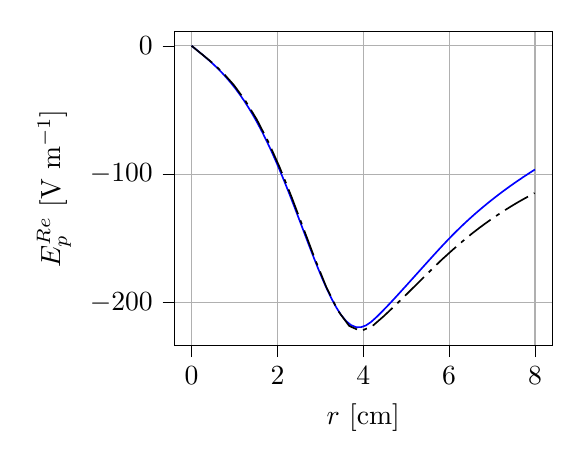
\begin{tikzpicture}

\definecolor{darkgray176}{RGB}{176,176,176}

\begin{axis}[
legend cell align=left,
legend pos= north east,
scale = .7,
ylabel = {$E_p^{Re}$ [V m$^{-1}$]},
xlabel = {$r$ [cm]},
tick align=outside,
tick pos=left,
x grid style={darkgray176},
xmajorgrids,
xmin=-0.399999991059303, xmax=8.39999981224537,
xtick style={color=black},
y grid style={darkgray176},
ymajorgrids,
ymin=-233.487666115471, ymax=11.1186479292325,
ytick style={color=black}
]
\addplot [semithick, blue]
table {%
0 0.000179109018722769
0.007999999797903 -0.215432547400165
0.015999999595806 -0.431044189095243
0.023999999393709 -0.646655816066035
0.031999999191612 -0.862267428312064
0.039999998989515 -1.07787902583285
0.047999998787418 -1.29349060862793
0.0560000014957041 -1.50910225513585
0.063999998383224 -1.72471373003903
0.0720000010915101 -1.94032534709313
0.07999999797903 -2.15593679254156
0.0880000006873161 -2.37154838013993
0.095999997574836 -2.58715979613171
0.104000000283122 -2.80367063274124
0.112000002991408 -3.02201557390387
0.119999994058162 -3.24036018259488
0.127999996766448 -3.45870509428096
0.135999999474734 -3.67704999122804
0.14400000218302 -3.89539487343565
0.151999993249774 -4.11373942316981
0.15999999595806 -4.33208427589706
0.167999998666346 -4.55042911388339
0.176000001374632 -4.76877393712835
0.183999992441386 -4.98711842789805
0.191999995149672 -5.20546322165883
0.199999986216426 -5.42380768294345
0.208000000566244 -5.64583994865852
0.215999991632998 -5.86978803806783
0.224000005982816 -6.09373676447936
0.23199999704957 -6.31768482434182
0.239999988116324 -6.54163286943018
0.248000002466142 -6.7655815515192
0.255999993532896 -6.98952956705786
0.26399998459965 -7.21347756782097
0.271999998949468 -7.43742620558318
0.279999990016222 -7.66137417679372
0.28800000436604 -7.88532278500233
0.295999995432794 -8.10927072665839
0.303999986499548 -8.33321865353652
0.312000000849366 -8.56543597497694
0.31999999191612 -8.79776158881733
0.327999982982874 -9.03008718783477
0.335999997332692 -9.26241344818595
0.343999988399446 -9.49473901755599
0.352000002749264 -9.72706524825872
0.359999993816018 -9.95939078797945
0.367999984882772 -10.1917163128748
0.37599999923259 -10.4240424991013
0.383999990299344 -10.6563679943445
0.392000004649162 -10.8886941509177
0.399999972432852 -11.12101894035
0.40799998678267 -11.3568385012463
0.416000001132488 -11.6002201602598
0.423999968916178 -11.843600387715
0.431999983265996 -12.0869820169417
0.439999997615814 -12.3303636312741
0.448000011965632 -12.5737452307119
0.455999979749322 -12.8171253985899
0.46399999409914 -13.060506968237
0.472000008448958 -13.303888522988
0.479999976232648 -13.547268646178
0.487999990582466 -13.7906501711354
0.496000004932284 -14.0340316811953
0.503999972715974 -14.2774117596929
0.511999987065792 -14.5295889666624
0.52000000141561 -14.7866074488958
0.5279999691993 -15.0436244201546
0.535999983549118 -15.3006428725216
0.543999997898936 -15.5576613099545
0.551999965682626 -15.8146782364116
0.559999980032444 -16.0716966439752
0.567999994382262 -16.3287150366033
0.57600000873208 -16.5857334142954
0.58399997651577 -16.8427502810101
0.591999990865588 -17.0997686288289
0.600000005215406 -17.3567869617104
0.607999972999096 -17.6138037836132
0.615999987348914 -17.8865250082861
0.624000001698732 -18.1596655864308
0.631999969482422 -18.4328045597102
0.63999998383224 -18.7059451078927
0.647999998182058 -18.9790856410934
0.655999965965748 -19.2522245694277
0.663999980315566 -19.5253650726634
0.671999994665384 -19.7985055609158
0.679999962449074 -20.0716444443005
0.687999976798892 -20.344784902585
0.69599999114871 -20.6179253458848
0.704000005498528 -20.8910657741993
0.711999973282218 -21.1698132944927
0.719999987632036 -21.461464970543
0.728000001981854 -21.7531166315821
0.735999969765544 -22.0447665799766
0.743999984115362 -22.3364182109919
0.75199999846518 -22.6280698269946
0.75999996624887 -22.9197197303515
0.767999980598688 -23.2113713163275
0.775999994948506 -23.5030228872894
0.784000009298325 -23.7946744432367
0.791999977082014 -24.0863242865366
0.799999944865704 -24.3779741148212
0.808000005781651 -24.6696273233541
0.81599997356534 -24.9744250296969
0.82399994134903 -25.2868787198254
0.832000002264977 -25.5993360323885
0.839999970048666 -25.9117896924773
0.847999937832355 -26.2242433375456
0.855999998748302 -26.5367006050464
0.863999966531992 -26.8491542200719
0.871999934315681 -27.1616078200755
0.879999995231628 -27.4740650425097
0.887999963015318 -27.7865186124677
0.896000023931265 -28.0989758048549
0.903999991714954 -28.4114293447653
0.911999959498644 -28.7238828696513
0.920000020414591 -29.0584433477106
0.92799998819828 -29.393897131268
0.93599995598197 -29.7293508998142
0.944000016897917 -30.06480855856
0.951999984681606 -30.4002622970822
0.959999952465296 -30.7357160205916
0.968000013381243 -31.0711736342987
0.975999981164932 -31.4066273277811
0.983999948948622 -31.7420810062494
0.992000009864569 -32.0775385749134
0.999999977648258 -32.4129922233518
1.00799994543195 -32.7484458567746
1.01600000634789 -33.0902575037578
1.02399997413158 -33.4508816152726
1.03199994191527 -33.8115056607813
1.04000000283122 -34.1721338385282
1.04799997061491 -34.5327577520603
1.0559999383986 -34.8933815996367
1.06399999931455 -35.2540095794575
1.07199996709824 -35.6146332951208
1.07999993488193 -35.9752569448693
1.08799999579787 -36.3358847268709
1.09599996358156 -36.6965082447641
1.10399993136525 -37.0571316967601
1.1119999922812 -37.4177592810963
1.11999996006489 -37.7852151549244
1.12800002098083 -38.1728552405559
1.13599998876452 -38.5604907461279
1.14399995654821 -38.9481261843434
1.15200001746416 -39.3357660679022
1.15999998524785 -39.723401371457
1.16799995303154 -40.111036607661
1.17600001394749 -40.4986762892629
1.18399998173118 -40.8863113909042
1.19199994951487 -41.2739464252081
1.20000001043081 -41.6615859049547
1.2079999782145 -42.04922080476
1.21599994599819 -42.4368556373198
1.22400000691414 -42.8306836385953
1.23199997469783 -43.2469815665902
1.23999994248152 -43.6632794260195
1.24800000339746 -44.0795820632592
1.25599997118115 -44.4958797855944
1.26399993896484 -44.9121774394201
1.27199999988079 -45.3284798710559
1.27999996766448 -45.7447773878488
1.28799993544817 -46.161074836173
1.29599999636412 -46.5773770623215
1.30399996414781 -46.9936743736765
1.3119999319315 -47.409971616579
1.31999999284744 -47.8262736373975
1.32799996063113 -48.2479099481181
1.33599992841482 -48.6940540975193
1.34399998933077 -49.1402033713703
1.35199995711446 -49.5863473820406
1.35999992489815 -50.032491323365
1.36799998581409 -50.4786403891953
1.37599995359778 -50.9247841918458
1.38400001451373 -51.3709331190283
1.39199998229742 -51.8170767831206
1.39999995008111 -52.2632203778722
1.40800001099706 -52.7093690972002
1.41599997878075 -53.1555125534555
1.42399994656444 -53.6016559404662
1.43200000748038 -54.0521410465773
1.43999997526407 -54.5288482188402
1.44799994304776 -55.005555321546
1.45600000396371 -55.4822679043296
1.4639999717474 -55.9589748679584
1.47199993953109 -56.4356817620912
1.48000000044703 -56.912394136293
1.48799996823072 -57.389100891405
1.49599993601441 -57.8658075770605
1.50399999693036 -58.3425197428056
1.51199996471405 -58.8192262895092
1.51999993249774 -59.2959327667699
1.52799999341369 -59.7726447242155
1.53599996119738 -60.2525831207479
1.54399992898107 -60.7601032361458
1.55199998989701 -61.2676291909691
1.5599999576807 -61.7751491685607
1.56800001859665 -62.2826749856012
1.57599989324808 -62.7901889171309
1.58399995416403 -63.2977145964163
1.59200001507998 -63.8052402068798
1.59999988973141 -64.3127539318751
1.60799995064735 -64.8202794046478
1.6160000115633 -65.3278048086432
1.62399988621473 -65.8353183271868
1.63199994713068 -66.3428435936016
1.64000000804663 -66.8524469758854
1.64799988269806 -67.3905565492871
1.65599994361401 -67.9286785845266
1.66400000452995 -68.4668005525792
1.67199987918139 -69.0049099244265
1.67999994009733 -69.5430317581723
1.68800000101328 -70.0811535247134
1.69599987566471 -70.6192626951179
1.70399993658066 -71.1573843274517
1.7119999974966 -71.6955058926107
1.71999987214804 -72.2336148616801
1.72799993306398 -72.7717362926836
1.73599999397993 -73.3098576566104
1.74399986863136 -73.8488921122532
1.75199992954731 -74.4169261093132
1.75999999046326 -74.9849600421814
1.7680000513792 -75.5529939108697
1.77599992603064 -76.1210144899235
1.78399998694658 -76.6890482303202
1.79200004786253 -77.2570819065118
1.79999992251396 -77.8251022931373
1.80799998342991 -78.3931358411332
1.81600004434586 -78.9611693249574
1.82399991899729 -79.5291895192591
1.83199997991323 -80.0972228749332
1.84000004082918 -80.6652561665325
1.84799991548061 -81.2332761686161
1.85599997639656 -81.8298985922981
1.86400003731251 -82.4266932357108
1.87199991196394 -83.0234739243227
1.87999997287989 -83.6202684483467
1.88800003379583 -84.217062912727
1.89599990844727 -84.8138434222776
1.90399996936321 -85.4106377672987
1.91200003027916 -86.0074320527039
1.91999990493059 -86.6042123833198
1.92799996584654 -87.2010065494375
1.93600002676249 -87.7978006559416
1.94399990141392 -88.3945808077555
1.95199996232986 -88.9913747950667
1.96000002324581 -89.6141472916213
1.96799989789724 -90.2380699415216
1.97599995881319 -90.8620070649905
1.98400001972914 -91.4859441349782
1.99199989438057 -92.1098666244783
1.99999995529652 -92.7338035875009
2.00800001621246 -93.357740497103
2.0159998908639 -93.9816628262435
2.02399995177984 -94.6055996289417
2.03200001269579 -95.2295363782496
2.03999988734722 -95.8534585470974
2.04799994826317 -96.4773951895903
2.05600000917912 -97.1013317786896
2.06399988383055 -97.7473451043956
2.07199994474649 -98.3960643349137
2.08000000566244 -99.0447836771642
2.08799988031387 -99.6934880269884
2.09599994122982 -100.342207592414
2.10400000214577 -100.990927269286
2.1119998767972 -101.639631953443
2.11999993771315 -102.288351852914
2.12799999862909 -102.937071863551
2.13599987328053 -103.585776881174
2.14399993419647 -104.234497113845
2.15199999511242 -104.883217457391
2.15999986976385 -105.531922807633
2.1679999306798 -106.187005456784
2.17599999159575 -106.857720750124
2.18399986624718 -107.528420516213
2.19199992716312 -108.199135987357
2.19999998807907 -108.86985154729
2.2079998627305 -109.54055157974
2.21599992364645 -110.211267317143
2.2239999845624 -110.881983142967
2.23199985921383 -111.552683441001
2.23999992012978 -112.223399443745
2.24799998104572 -112.894115534827
2.25600004196167 -113.564831714171
2.2639999166131 -114.23553236549
2.27199997752905 -114.906248721131
2.280000038445 -115.588545401131
2.28799991309643 -116.276838146134
2.29599997401237 -116.965146972545
2.30400003492832 -117.653455854503
2.31199990957975 -118.341748766141
2.3199999704957 -119.030057759051
2.32800003141165 -119.718366807377
2.33599990606308 -120.406659885215
2.34399996697903 -121.0949690442
2.35200002789497 -121.783278258448
2.35999990254641 -122.471571502088
2.36799996346235 -123.159880826725
2.3760000243783 -123.848190206486
2.38399989902973 -124.536816184348
2.39199995994568 -125.237378614705
2.40000002086163 -125.937941055772
2.40799989551306 -126.638487196423
2.415999956429 -127.339049658883
2.42400001734495 -128.039612132026
2.43199989199638 -128.740158304726
2.43999995291233 -129.440720799228
2.44800001382828 -130.141283304345
2.45599988847971 -130.841829509012
2.46399994939566 -131.542392035434
2.4720000103116 -132.242954572486
2.47999988496304 -132.943500809039
2.48799994587898 -133.644063367321
2.49600000679493 -134.34699234883
2.50399988144636 -135.053514845311
2.51199994236231 -135.760053745144
2.52000000327826 -136.466592598104
2.52799987792969 -137.173114953965
2.53599993884563 -137.879653713295
2.54399999976158 -138.586192425948
2.55199987441301 -139.292714641618
2.55999993532896 -139.999253260647
2.56799999624491 -140.705791833189
2.57599987089634 -141.412313908875
2.58399993181229 -142.118852388259
2.59199999272823 -142.825390821122
2.59999986737967 -143.531912757251
2.60799992829561 -144.237505192656
2.61599998921156 -144.942806397751
2.62399986386299 -145.648091063177
2.63199992477894 -146.353392031924
2.63999998569489 -147.058692882645
2.64799986034632 -147.763977194002
2.65599992126226 -148.469277808969
2.66399998217821 -149.174578306205
2.67199985682964 -149.879862264382
2.67999991774559 -150.585162526456
2.68799997866154 -151.290462671097
2.69599985331297 -151.995746276981
2.70399991422892 -152.701046187049
2.71199997514486 -153.405094657121
2.7199998497963 -154.10099052121
2.72799991071224 -154.796902383725
2.73599997162819 -155.492814041993
2.74399984627962 -156.188709293358
2.75199990719557 -156.884620543646
2.75999996811152 -157.580531590403
2.76800002902746 -158.276442433228
2.77599990367889 -158.972336869967
2.78399996459484 -159.668247306335
2.79200002551079 -160.364157539645
2.79999990016222 -161.060051367276
2.80799996107817 -161.755961194985
2.81600002199411 -162.451870820144
2.82399989664555 -163.138492854997
2.83199995756149 -163.815926831538
2.84000001847744 -164.493360501822
2.84799989312887 -165.170778093506
2.85599995404482 -165.848211152051
2.86400001496077 -166.525643905104
2.8719998896122 -167.203060580382
2.87999995052814 -167.88049272338
2.88800001144409 -168.557924561289
2.89599988609552 -169.235340322363
2.90399994701147 -169.912771551778
2.91200000792742 -170.590202477223
2.91999988257885 -171.267617326412
2.9279999434948 -171.945047644679
2.93600000441074 -172.597674661522
2.94399987906218 -173.24658907244
2.95199993997812 -173.895518167599
2.96000000089407 -174.544446838393
2.9679998755455 -175.193359976256
2.97599993646145 -175.842287799386
2.9839999973774 -176.491215199207
2.99199987202883 -177.140127067177
2.99999993294477 -177.789053621438
3.00799999386072 -178.43797975344
3.01599986851215 -179.086890354674
3.0239999294281 -179.735815643215
3.03199999034405 -180.384740510545
3.03999986499548 -181.024233205147
3.04799992591143 -181.63369527409
3.05599998682737 -182.243156781748
3.06399986147881 -182.852603538579
3.07199992239475 -183.462063925068
3.0799999833107 -184.071523751661
3.08799985796213 -184.680968828982
3.09599991887808 -185.290427537123
3.10399997979403 -185.899885686745
3.11199985444546 -186.509329088459
3.1199999153614 -187.118786122521
3.12799997627735 -187.728242599454
3.1360000371933 -188.337698519717
3.14400009810925 -188.947153883767
3.15199978649616 -189.550043885473
3.15999984741211 -190.102773380803
3.16799990832806 -190.655502994862
3.175999969244 -191.208232727279
3.18400003015995 -191.760962577681
3.1920000910759 -192.313692545698
3.19999977946281 -192.866396892654
3.20799984037876 -193.41912709479
3.21599990129471 -193.97185741344
3.22399996221066 -194.524587848239
3.2320000231266 -195.077318398825
3.24000008404255 -195.630049064836
3.24799977242947 -196.182754107574
3.25599983334541 -196.735485003354
3.26399989426136 -197.271039652545
3.27199995517731 -197.766268592287
3.28000001609325 -198.261497670939
3.2880000770092 -198.756726888071
3.29599976539612 -199.251933182513
3.30399982631207 -199.747162675314
3.31199988722801 -200.242392305315
3.31999994814396 -200.737622072119
3.32800000905991 -201.232851975221
3.33600006997585 -201.728082014285
3.34399975836277 -202.223289128086
3.35199981927872 -202.718519437758
3.35999988019466 -203.213749882115
3.36799994111061 -203.708980460744
3.37600000202656 -204.204211173231
3.3840000629425 -204.620452770947
3.39199975132942 -205.035918056635
3.39999981224537 -205.451402841345
3.40799987316132 -205.866887777254
3.41599993407726 -206.282372863901
3.42399999499321 -206.697858100827
3.43200005590916 -207.113343487605
3.43999974429607 -207.52880967628
3.44799980521202 -207.944295361299
3.45599986612797 -208.35978119478
3.46399992704391 -208.775267176272
3.47199998795986 -209.190753305326
3.48000004887581 -209.606239581497
3.48799973726273 -210.02170665689
3.49599979817867 -210.371893546994
3.50399985909462 -210.69166622974
3.51199992001057 -211.011439069692
3.51999998092651 -211.331212066375
3.52800004184246 -211.650985219318
3.53600010275841 -211.970758528054
3.54399979114532 -212.29051710161
3.55199985206127 -212.610290720521
3.55999991297722 -212.930064493826
3.56799997389317 -213.249838421064
3.57600003480911 -213.569612501775
3.58400009572506 -213.889386735501
3.59199978411198 -214.20914623124
3.59999984502792 -214.528920769621
3.60799990594387 -214.809274373397
3.61599996685982 -215.023643967967
3.62400002777576 -215.238013717637
3.63200008869171 -215.452383621947
3.63999977707863 -215.666743698127
3.64799983799458 -215.881113910337
3.65599989891052 -216.095484275816
3.66399995982647 -216.309854794113
3.67200002074242 -216.524225464775
3.68000008165836 -216.738596287354
3.68799977004528 -216.952957279047
3.69599983096123 -217.16732840411
3.70399989187717 -217.381699679751
3.71199995279312 -217.596071105529
3.72000001370907 -217.803289379204
3.72800007462502 -217.908841082792
3.73599976301193 -218.014388016072
3.74399982392788 -218.119940008828
3.75199988484383 -218.225492145538
3.75999994575977 -218.331044425781
3.76800000667572 -218.436596849139
3.77600006759167 -218.542149415195
3.78399975597858 -218.647697208382
3.79199981689453 -218.753250058578
3.79999987781048 -218.85880305023
3.80799993872643 -218.964356182925
3.81599999964237 -219.069909456255
3.82400006055832 -219.175462869813
3.83199974894524 -219.281011508005
3.83999980986118 -219.306311217328
3.84799987077713 -219.305906654522
3.85599993169308 -219.305502217798
3.86399999260902 -219.305097906792
3.87200005352497 -219.304693721142
3.87999974191189 -219.304289679299
3.88799980282784 -219.303885743272
3.89599986374378 -219.303481931523
3.90399992465973 -219.303078243694
3.91199998557568 -219.302674679429
3.92000004649162 -219.302271238375
3.92799973487854 -219.301867938957
3.93599979579449 -219.301464743262
3.94399985671043 -219.301061669724
3.95199991762638 -219.257175227185
3.95999997854233 -219.159952010608
3.96800003945827 -219.06272889341
3.97599972784519 -218.96551040257
3.98399978876114 -218.868287483275
3.99199984967709 -218.771064662513
3.99999991059303 -218.673841940004
4.00799997150898 -218.576619315469
4.01600003242493 -218.479396788631
4.02400009334087 -218.382174359213
4.03199978172779 -218.28495655417
4.03999984264374 -218.187734318762
4.04799990355968 -218.090512179952
4.05599996447563 -217.993290137466
4.06400002539158 -217.884605861012
4.07200008630753 -217.705978024056
4.07999977469444 -217.527358569487
4.08799983561039 -217.348730861245
4.09599989652634 -217.17010321709
4.10399995744228 -216.991475636843
4.11200001835823 -216.812848120325
4.12000007927418 -216.634220667357
4.12799976766109 -216.455601595683
4.13599982857704 -216.276974269281
4.14399988949299 -216.098347005898
4.15199995040894 -215.919719805359
4.16000001132488 -215.741092667489
4.16800007224083 -215.562465592112
4.17599976062775 -215.38384689696
4.18399982154369 -215.155511132837
4.19199988245964 -214.917168931818
4.19999994337559 -214.678826751861
4.20800000429153 -214.440484592905
4.21600006520748 -214.202142454894
4.2239997535944 -213.963811436355
4.23199981451035 -213.725469340058
4.23999987542629 -213.487127264533
4.24799993634224 -213.248785209722
4.25599999725819 -213.010443175567
4.26400005817413 -212.772101162013
4.27199974656105 -212.533770267581
4.279999807477 -212.295428295057
4.28799986839294 -212.057086342963
4.29599992930889 -211.83024875334
4.30399999022484 -211.567817474621
4.31200005114079 -211.305386179889
4.3199997395277 -211.042967089417
4.32799980044365 -210.780535762528
4.3359998613596 -210.518104419492
4.34399992227554 -210.255673060267
4.35199998319149 -209.993241684806
4.36000004410744 -209.730810293064
4.36799973249435 -209.468391105319
4.3759997934103 -209.205959680883
4.38399985432625 -208.94352824003
4.3919999152422 -208.681096782715
4.39999997615814 -208.418665308892
4.40800003707409 -208.152152859167
4.41599972546101 -207.878199143601
4.42399978637695 -207.604232681065
4.4319998472929 -207.330266229049
4.43999990820885 -207.056299787584
4.44799996912479 -206.782333356698
4.45600003004074 -206.508366936421
4.46399971842766 -206.234413284241
4.47199977934361 -205.960446885272
4.47999984025955 -205.686480497002
4.4879999011755 -205.41251411946
4.49599996209145 -205.138547752678
4.50400002300739 -204.864581396685
4.51200008392334 -204.590615051513
4.51999977231026 -204.315098042633
4.5279998332262 -204.032613370831
4.53599989414215 -203.750128727844
4.5439999550581 -203.467644113753
4.55200001597404 -203.18515952864
4.56000007688999 -202.902674972587
4.56799976527691 -202.620203599786
4.57599982619286 -202.337719102112
4.5839998871088 -202.055234633722
4.59199994802475 -201.772750194737
4.6000000089407 -201.490265785227
4.60800006985664 -201.207781405277
4.61599975824356 -200.925310209074
4.62399981915951 -200.642825888496
4.63199988007545 -200.360341597732
4.6399999409914 -200.071791264397
4.64800000190735 -199.783321332777
4.6560000628233 -199.49485144139
4.66399975121021 -199.206395023171
4.67199981212616 -198.917925212594
4.67999987304211 -198.629455442597
4.68799993395805 -198.340985713305
4.695999994874 -198.052516024813
4.70400005578995 -197.764046377261
4.71199974417686 -197.47559020357
4.71999980509281 -197.187120638236
4.72799986600876 -196.898651114191
4.73599992692471 -196.610181631554
4.74399998784065 -196.321712190445
4.7520000487566 -196.029922253814
4.75999973714352 -195.737529494307
4.76799979805946 -195.445123164518
4.77599985897541 -195.152716880711
4.78399991989136 -194.86031064302
4.7919999808073 -194.567904451579
4.80000004172325 -194.275498306524
4.80799973011017 -193.983105824105
4.81599979102612 -193.690699772226
4.82399985194206 -193.39829376714
4.83199991285801 -193.105887808985
4.83999997377396 -192.813481897898
4.8480000346899 -192.521076034019
4.85599972307682 -192.228683833587
4.86399978399277 -191.93468045501
4.87199984490871 -191.63990248549
4.87999990582466 -191.345124563203
4.88799996674061 -191.050346688289
4.89600002765656 -190.755568860889
4.90399971604347 -190.460804807696
4.91199977695942 -190.166027075741
4.91999983787537 -189.871249391722
4.92799989879131 -189.576471755782
4.93599995970726 -189.281694168062
4.94400002062321 -188.986916628707
4.95199970901012 -188.692152864402
4.95999976992607 -188.397375422205
4.96799983084202 -188.102598028806
4.97599989175797 -187.807170282903
4.98399995267391 -187.511101627245
4.99200001358986 -187.215033017676
4.99999970197678 -186.918978240995
5.00799976289272 -186.622909724017
5.01599982380867 -186.326841253544
5.02399988472462 -186.030772829716
5.03199994564056 -185.734704452672
5.04000000655651 -185.438636122553
5.04800006747246 -185.142567839502
5.05599975585938 -184.846513390304
5.06399981677532 -184.550445201809
5.07199987769127 -184.254377060808
5.07999993860722 -183.958308967444
5.08799999952316 -183.662009044492
5.09600006043911 -183.365246734347
5.10399974882603 -183.068498287476
5.11199980974197 -182.771736066083
5.11999987065792 -182.474973889268
5.12799993157387 -182.178211757169
5.13599999248981 -181.881449669919
5.14400005340576 -181.584687627657
5.15199974179268 -181.287939449471
5.15999980270863 -180.991177497594
5.16799986362457 -180.694415591117
5.17599992454052 -180.39765373018
5.18399998545647 -180.100891914922
5.19200004637241 -179.804130145483
5.19999973475933 -179.507286742399
5.20799979567528 -179.209943994647
5.21599985659122 -178.912601290942
5.22399991750717 -178.615258631419
5.23199997842312 -178.317916016214
5.24000003933907 -178.020573445465
5.24799972772598 -177.723244765292
5.25599978864193 -177.425902283873
5.26399984955788 -177.128559847304
5.27199991047382 -176.831217455752
5.27999997138977 -176.533875109347
5.28800003230572 -176.23653280823
5.29599972069263 -175.939204398512
5.30399978160858 -175.641862188391
5.31199984252453 -175.34452002398
5.31999990344048 -175.046231165267
5.32799996435642 -174.74793750135
5.33600002527237 -174.449643885305
5.34399971365929 -174.151364207551
5.35199977457523 -173.853070687698
5.35999983549118 -173.554777216168
5.36799989640713 -173.256483793125
5.37599995732307 -172.958190418684
5.38400001823902 -172.659897093035
5.39199970662594 -172.361617706575
5.39999976754189 -172.063324478944
5.40799982845783 -171.765031300555
5.41599988937378 -171.466738171563
5.42399995028973 -171.168445092125
5.43200001120567 -170.872123927003
5.43999969959259 -170.575922203493
5.44799976050854 -170.279706681505
5.45599982142448 -169.983491154539
5.46399988234043 -169.687275622591
5.47199994325638 -169.391060085656
5.48000000417233 -169.094844543733
5.48799969255924 -168.798642790313
5.49599975347519 -168.502427238392
5.50399981439114 -168.206211681465
5.51199987530708 -167.90999611953
5.51999993622303 -167.613780552581
5.52799999713898 -167.317564980614
5.53600005805492 -167.021776903698
5.54399974644184 -166.726323408403
5.55199980735779 -166.430856150174
5.55999986827374 -166.13538888767
5.56799992918968 -165.839921620887
5.57599999010563 -165.544454349821
5.58400005102158 -165.248987074468
5.59199973940849 -164.953533553487
5.59999980032444 -164.658066269549
5.60799986124039 -164.362598981313
5.61599992215633 -164.067131688775
5.62399998307228 -163.771664391931
5.63200004398823 -163.476197090777
5.63999973237514 -163.181587748867
5.64799979329109 -162.888784124199
5.65599985420704 -162.595980495893
5.66399991512299 -162.303176863944
5.67199997603893 -162.010373228351
5.68000003695488 -161.717569589108
5.6879997253418 -161.424779580854
5.69599978625774 -161.131975934347
5.70399984717369 -160.839172284088
5.71199990808964 -160.546368630219
5.71999996900558 -160.253564972686
5.72800002992153 -159.960761311486
5.73599971830845 -159.667971281243
5.7439997792244 -159.37543560961
5.75199984014034 -159.08691025127
5.75999990105629 -158.798384889837
5.76799996197224 -158.50985952531
5.77600002288818 -158.221334157684
5.7839997112751 -157.932822222365
5.79199977219105 -157.644296848571
5.79999983310699 -157.355771471622
5.80799989402294 -157.067246091557
5.81599995493889 -156.778720708401
5.82400001585484 -156.490195322131
5.83199970424175 -156.201683368152
5.8399997651577 -155.913157975645
5.84799982607365 -155.624632580015
5.85599988698959 -155.340627753761
5.86399994790554 -155.057694646649
5.87200000882149 -154.77476153688
5.8799996972084 -154.49184159945
5.88799975812435 -154.208908484358
5.8959998190403 -153.925975366601
5.90399987995625 -153.643042246181
5.91199994087219 -153.360109123084
5.92000000178814 -153.077175997319
5.92799969017506 -152.794256043879
5.935999751091 -152.511322912763
5.94399981200695 -152.228389778967
5.9519998729229 -151.94545664249
5.95999993383884 -151.666183608177
5.96799999475479 -151.389856171303
5.97599968314171 -151.113541599477
5.98399974405766 -150.837214157893
5.9919998049736 -150.560886713952
5.99999986588955 -150.28455926765
6.0079999268055 -150.008231818987
6.01599998772144 -149.731904367959
6.02400004863739 -149.455576914564
6.03199973702431 -149.179262326203
6.03999979794025 -148.90293486807
6.0479998588562 -148.626607407563
6.05599991977215 -148.350279944682
6.0639999806881 -148.076146623389
6.07200004160404 -147.807137518838
6.07999972999096 -147.538140938701
6.08799979090691 -147.269131829742
6.09599985182285 -147.000122718575
6.1039999127388 -146.731113605199
6.11199997365475 -146.462104489623
6.12000003457069 -146.193095371858
6.12799972295761 -145.924098778413
6.13599978387356 -145.65508965618
6.14399984478951 -145.386080531728
6.15199990570545 -145.117071405054
6.1599999666214 -144.848062276157
6.16800002753735 -144.579405292172
6.17599971592426 -144.318138796449
6.18399977684021 -144.056860131848
6.19199983775616 -143.795581465012
6.1999998986721 -143.534302795937
6.20799995958805 -143.273024124623
6.216000020504 -143.011745451101
6.22399970889091 -142.750478941927
6.23199976980686 -142.489200263863
6.23999983072281 -142.227921583568
6.24799989163876 -141.966642901022
6.2559999525547 -141.705364216225
6.26399964094162 -141.444097695817
6.2720000743866 -141.182806839864
6.27999976277351 -140.927745181508
6.28800019621849 -140.674296515637
6.29599988460541 -140.420871450263
6.30399957299232 -140.167446382415
6.3120000064373 -139.913997709123
6.31999969482422 -139.660572636321
6.3280001282692 -139.407123958073
6.33599981665611 -139.153698880305
6.34399950504303 -138.900273800056
6.35199993848801 -138.64682511435
6.35999962687492 -138.393400029123
6.3680000603199 -138.139951338436
6.37599974870682 -137.886526248224
6.38400018215179 -137.637187426813
6.39199987053871 -137.391414608288
6.39999955892563 -137.145641786824
6.40799999237061 -136.899846072149
6.41599968075752 -136.654073244801
6.4240001142025 -136.408277524236
6.43199980258942 -136.162504690993
6.43999949097633 -135.916731854796
6.44799992442131 -135.670936125375
6.45599961280823 -135.425163283268
6.4640000462532 -135.17936754793
6.47199973464012 -134.9335946999
6.4800001680851 -134.687798958633
6.48799985647202 -134.443589687522
6.49599954485893 -134.204561209626
6.50399997830391 -133.965510441584
6.51199966669083 -133.726481907666
6.5200001001358 -133.487431083568
6.52799978852272 -133.248402493582
6.5360002219677 -133.009351613425
6.54399991035461 -132.770322967377
6.55199959874153 -132.531294293293
6.56000003218651 -132.292243329018
6.56799972057343 -132.053214598826
6.5760001540184 -131.814163578439
6.58399984240532 -131.575134792151
6.59199953079224 -131.340009488934
6.59999996423721 -131.107417681593
6.60799965262413 -130.874847506853
6.61600008606911 -130.642255643464
6.62399977445602 -130.409685412659
6.632000207901 -130.177093493182
6.63999989628792 -129.944523206305
6.64799958467484 -129.711952891387
6.65600001811981 -129.479360887779
6.66399970650673 -129.246790516765
6.67200013995171 -129.014198457023
6.67999982833862 -128.781628029884
6.68799951672554 -128.549057574681
6.69599995017052 -128.322189036045
6.70399963855743 -128.095798896532
6.71200007200241 -127.869387643989
6.71999976038933 -127.642997448473
6.7280001938343 -127.416586139901
6.73599988222122 -127.190195888378
6.74399957060814 -126.963805608847
6.75200000405312 -126.737394216241
6.75999969244003 -126.511003880679
6.76800012588501 -126.284592432028
6.77599981427193 -126.058202040391
6.78399950265884 -125.83181162074
6.79199993610382 -125.606865397488
6.79999962449074 -125.386389751193
6.80800005793571 -125.165893542796
6.81599974632263 -124.9454178407
6.82400017976761 -124.724921576469
6.83199986815453 -124.504445818526
6.83999955654144 -124.283970032665
6.84799998998642 -124.063473684672
6.85599967837334 -123.842997842962
6.86400011181831 -123.622501439106
6.87199980020523 -123.40202554151
6.87999948859215 -123.181549615985
6.88799992203712 -122.961053128292
6.89599961042404 -122.743801163456
6.90400004386902 -122.528967300201
6.91199973225594 -122.314153416029
6.92000016570091 -122.099319497183
6.92799985408783 -121.884505557402
6.93599954247475 -121.669691589816
6.94399997591972 -121.454857587529
6.95199966430664 -121.240043564319
6.96000009775162 -121.025209506395
6.96799978613853 -120.810395427546
6.97599947452545 -120.59558132085
6.98399990797043 -120.38074717943
6.99199959635735 -120.165933017078
7.00000002980232 -119.955930954385
7.00799971818924 -119.74653895384
7.01600015163422 -119.537127423753
7.02399984002113 -119.327735367909
7.03199952840805 -119.118343284416
7.03999996185303 -118.90893167135
7.04799965023994 -118.699539532546
7.05600008368492 -118.490127864155
7.06399977207184 -118.280735670023
7.07200020551682 -118.071323946292
7.07999989390373 -117.861931696791
7.08799958229065 -117.652539419626
7.09600001573563 -117.444233526997
7.10399970412254 -117.240036297976
7.11200013756752 -117.035820023394
7.11999982595444 -116.831622739445
7.12799951434135 -116.627425428004
7.13599994778633 -116.423209070985
7.14399963617325 -116.219011704584
7.15200006961823 -116.014795292593
7.15999975800514 -115.810597871218
7.16800019145012 -115.606381404238
7.17599987983704 -115.402183927854
7.18399956822395 -115.197986423977
7.19200000166893 -114.993769874473
7.19999969005585 -114.792235050256
7.20800012350082 -114.592999705664
7.21599981188774 -114.39378288803
7.22399950027466 -114.194566043127
7.23199993371964 -113.995330616687
7.23999962210655 -113.796113717203
7.24800005555153 -113.596878236186
7.25599974393845 -113.397661282122
7.26400017738342 -113.198425746511
7.27199986577034 -112.99920873785
7.27999955415726 -112.799991701866
7.28799998760223 -112.600756084325
7.29599967598915 -112.401538993727
7.30400010943413 -112.206396486013
7.31199979782104 -112.011958628552
7.31999948620796 -111.817520744031
7.32799991965294 -111.623064723266
7.33599960803986 -111.428626784569
7.34400004148483 -111.234170709637
7.35199972987175 -111.03973271677
7.36000016331673 -110.845276587655
7.36799985170364 -110.650838540602
7.37599954009056 -110.456400466451
7.38399997353554 -110.26194425601
7.39199966192245 -110.067506127639
7.40000009536743 -109.87386792338
7.40799978375435 -109.684020325068
7.41599947214127 -109.494172699901
7.42399990558624 -109.304307366257
7.43199959397316 -109.114459687363
7.44000002741814 -108.924594299969
7.44799971580505 -108.73474656734
7.45600014925003 -108.5448811262
7.46399983763695 -108.355033339822
7.47199952602386 -108.165185526564
7.47999995946884 -107.97532000476
7.48799964785576 -107.785472137719
7.49600008130074 -107.595606562133
7.50399976968765 -107.407053527318
7.51200020313263 -107.219781316405
7.51999989151955 -107.032826166399
7.52799957990646 -106.846290481581
7.53600001335144 -106.6599756432
7.54399970173836 -106.474154584882
7.55200013518333 -106.28849370314
7.55999982357025 -106.103382501925
7.56799951195717 -105.91838878116
7.57599994540215 -105.733965520216
7.58399963378906 -105.549617798818
7.59200006723404 -105.365895333933
7.59999975562096 -105.182189978609
7.60800018906593 -104.999163597916
7.61599987745285 -104.81615428322
7.62399956583977 -104.633778718189
7.63199999928474 -104.451443800737
7.63999968767166 -104.26969841663
7.64800012111664 -104.088050631855
7.65599980950356 -103.906931610267
7.66399949789047 -103.725983199375
7.67199993133545 -103.545469756283
7.67999961972237 -103.365199114081
7.68800005316734 -103.185304955366
7.69599974155426 -103.005708461291
7.70400017499924 -102.826430124014
7.71199986338615 -102.647503341903
7.71999955177307 -102.468853746145
7.72799998521805 -102.290575672958
7.73599967360497 -102.11253460626
7.74400010704994 -101.934917860862
7.75199979543686 -101.757481879671
7.75999948382378 -101.580538609848
7.76799991726875 -101.403687630563
7.77599960565567 -101.227396999285
7.78400003910065 -101.051144012435
7.79199972748756 -100.875502075543
7.80000016093254 -100.699843780084
7.80799984931946 -100.524846323431
7.81599953770638 -100.349848853813
7.82399997115135 -100.175422025403
7.83199965953827 -100.001064831566
7.84000009298325 -99.8272217883717
7.84799978137016 -99.6535010362508
7.85599946975708 -99.4802545824298
7.86399990320206 -99.307150138565
7.87199959158897 -99.1344807014467
7.88000002503395 -98.9620046691584
7.88799971342087 -98.7899090550473
7.89600014686584 -98.6180577047422
7.90399983525276 -98.4465326679799
7.91199952363968 -98.2753179421102
7.91999995708466 -98.1043442158263
7.92799964547157 -97.9337461444619
7.93600007891655 -97.7633365424645
7.94399976730347 -97.5933515028202
7.95199945569038 -97.4235187122378
7.95999988913536 -97.254127035925
7.96799957752228 -97.084851986681
7.97600001096725 -96.9160656490382
7.98399969935417 -96.7473451567642
7.99200013279915 -96.5791606413182
7.99999982118607 -96.4109917884273
};
\addplot [semithick, black, dash pattern=on 9.6pt off 2.4pt on 1.5pt off 2.4pt]
table {%
0 0
0.00800800800800801 -0.215520094371126
0.016016016016016 -0.431040188742253
0.024024024024024 -0.646560283113379
0.032032032032032 -0.864786084219384
0.04004004004004 -1.08452391999653
0.048048048048048 -1.30426175577368
0.0560560560560561 -1.52399959155082
0.0640640640640641 -1.74373742732797
0.0720720720720721 -1.96347526310512
0.0800800800800801 -2.18321309888226
0.0880880880880881 -2.40295093465941
0.0960960960960961 -2.62268877043656
0.104104104104104 -2.84242660621371
0.112112112112112 -3.06216444199085
0.12012012012012 -3.281902277768
0.128128128128128 -3.50164011354515
0.136136136136136 -3.72137794932229
0.144144144144144 -3.94111578509944
0.152152152152152 -4.16085362087659
0.16016016016016 -4.38059145665373
0.168168168168168 -4.60032929243088
0.176176176176176 -4.81844965500502
0.184184184184184 -5.03396974937615
0.192192192192192 -5.24948984374728
0.2002002002002 -5.46501226575704
0.208208208208208 -5.68062547009153
0.216216216216216 -5.89623867442603
0.224224224224224 -6.11185187876052
0.232232232232232 -6.32746508309502
0.24024024024024 -6.54704121753787
0.248248248248248 -6.76663804092713
0.256256256256256 -6.98623486431638
0.264264264264264 -7.20583168770562
0.272272272272272 -7.42542851109488
0.28028028028028 -7.64502533448413
0.288288288288288 -7.86462215787338
0.296296296296296 -8.08421898126263
0.304304304304304 -8.30381580465188
0.312312312312312 -8.52341262804113
0.32032032032032 -8.74300945143038
0.328328328328328 -8.96260627481963
0.336336336336336 -9.18220309820888
0.344344344344344 -9.40179992159813
0.352352352352352 -9.62139674498738
0.36036036036036 -9.84099356837663
0.368368368368368 -10.0605903917659
0.376376376376376 -10.2801872151551
0.384384384384384 -10.4997840385444
0.392392392392392 -10.7193808619336
0.4004004004004 -10.9389776853229
0.408408408408408 -11.1582351337809
0.416416416416416 -11.3738483381154
0.424424424424424 -11.5894615424499
0.432432432432432 -11.8050747467844
0.44044044044044 -12.0221218875713
0.448448448448448 -12.263806522639
0.456456456456456 -12.5054911577067
0.464464464464464 -12.7471757927743
0.472472472472473 -12.988860427842
0.48048048048048 -13.2326465126813
0.488488488488488 -13.4782535746668
0.496496496496497 -13.7238606366522
0.504504504504504 -13.9694676986377
0.512512512512513 -14.2150747606232
0.520520520520521 -14.4606818226086
0.528528528528528 -14.7062888845941
0.536536536536537 -14.9518959465796
0.544544544544545 -15.197503008565
0.552552552552553 -15.4431100705505
0.560560560560561 -15.6887171325359
0.568568568568569 -15.9343241945214
0.576576576576577 -16.1799312565069
0.584584584584585 -16.4255383184923
0.592592592592593 -16.6711453804778
0.600600600600601 -16.9167524424632
0.608608608608609 -17.1623595044487
0.616616616616617 -17.4079665664342
0.624624624624625 -17.6535736284196
0.632632632632633 -17.8991806904051
0.640640640640641 -18.1447877523905
0.648648648648649 -18.390394814376
0.656656656656657 -18.6360018763615
0.664664664664665 -18.8816089383469
0.672672672672673 -19.1272160003324
0.680680680680681 -19.3690283025439
0.688688688688689 -19.6107129376116
0.696696696696697 -19.8523975726792
0.704704704704705 -20.0940822077469
0.712712712712713 -20.3602566819536
0.720720720720721 -20.6565812388945
0.728728728728729 -20.9529057958354
0.736736736736737 -21.2492303527763
0.744744744744745 -21.5455549097173
0.752752752752753 -21.8455817652198
0.760760760760761 -22.1458917611493
0.768768768768769 -22.4462017570788
0.776776776776777 -22.7465117530084
0.784784784784785 -23.0468217489379
0.792792792792793 -23.3471317448674
0.800800800800801 -23.6474417407969
0.808808808808809 -23.9477517367265
0.816816816816817 -24.248061732656
0.824824824824825 -24.5483717285855
0.832832832832833 -24.8486817245151
0.840840840840841 -25.1489917204446
0.848848848848849 -25.4493017163741
0.856856856856857 -25.7496117123037
0.864864864864865 -26.0499217082332
0.872872872872873 -26.3502317041627
0.880880880880881 -26.6505417000923
0.888888888888889 -26.9508516960218
0.896896896896897 -27.2511616919513
0.904904904904905 -27.5514716878809
0.912912912912913 -27.8517816838104
0.920920920920921 -28.1520916797399
0.928928928928929 -28.4524016756695
0.936936936936937 -28.752711671599
0.944944944944945 -29.0515842956696
0.952952952952953 -29.3479088526105
0.960960960960961 -29.6442334095514
0.968968968968969 -29.9405579664923
0.976976976976977 -30.2368825234332
0.984984984984985 -30.5874710101067
0.992992992992993 -30.9482873843382
1.001001001001 -31.3091037585697
1.00900900900901 -31.6699201328011
1.01701701701702 -32.0319832606664
1.02502502502503 -32.3966696068163
1.03303303303303 -32.7613559529662
1.04104104104104 -33.1260422991161
1.04904904904905 -33.490728645266
1.05705705705706 -33.8554149914159
1.06506506506507 -34.2201013375659
1.07307307307307 -34.5847876837158
1.08108108108108 -34.9494740298657
1.08908908908909 -35.3141603760156
1.0970970970971 -35.6788467221655
1.10510510510511 -36.0435330683154
1.11311311311311 -36.4082194144653
1.12112112112112 -36.7729057606153
1.12912912912913 -37.1375921067652
1.13713713713714 -37.5022784529151
1.14514514514515 -37.866964799065
1.15315315315315 -38.2316511452149
1.16116116116116 -38.5963374913648
1.16916916916917 -38.9610238375147
1.17717717717718 -39.3257101836647
1.18518518518519 -39.6903965298146
1.19319319319319 -40.0550828759645
1.2012012012012 -40.4197692221144
1.20920920920921 -40.7844555682643
1.21721721721722 -41.1462244791273
1.22522522522523 -41.5070408533588
1.23323323323323 -41.8678572275902
1.24124124124124 -42.2286736018217
1.24924924924925 -42.6072979481408
1.25725725725726 -43.0440164256853
1.26526526526527 -43.4807349032298
1.27327327327327 -43.9174533807743
1.28128128128128 -44.3541718583188
1.28928928928929 -44.79347778136
1.2972972972973 -45.2338131892861
1.30530530530531 -45.6741485972121
1.31331331331331 -46.1144840051382
1.32132132132132 -46.5548194130642
1.32932932932933 -46.9951548209903
1.33733733733734 -47.4354902289164
1.34534534534535 -47.8758256368424
1.35335335335335 -48.3161610447685
1.36136136136136 -48.7564964526945
1.36936936936937 -49.1968318606206
1.37737737737738 -49.6371672685467
1.38538538538539 -50.0775026764727
1.39339339339339 -50.5178380843988
1.4014014014014 -50.9581734923248
1.40940940940941 -51.3985089002509
1.41741741741742 -51.838844308177
1.42542542542543 -52.279179716103
1.43343343343343 -52.7195151240291
1.44144144144144 -53.1598505319552
1.44944944944945 -53.6001859398812
1.45745745745746 -54.0405213478073
1.46546546546547 -54.4808567557333
1.47347347347347 -54.9211921636594
1.48148148148148 -55.3609956138148
1.48948948948949 -55.7977140913594
1.4974974974975 -56.2344325689039
1.50550550550551 -56.6711510464484
1.51351351351351 -57.1078695239929
1.52152152152152 -57.5958078988476
1.52952952952953 -58.1141091586314
1.53753753753754 -58.6324104184151
1.54554554554555 -59.1507116781988
1.55355355355355 -59.6693552376839
1.56156156156156 -60.1908090028415
1.56956956956957 -60.7122627679991
1.57757757757758 -61.2337165331567
1.58558558558559 -61.7551702983144
1.59359359359359 -62.276624063472
1.6016016016016 -62.7980778286296
1.60960960960961 -63.3195315937872
1.61761761761762 -63.8409853589448
1.62562562562563 -64.3624391241025
1.63363363363363 -64.8838928892601
1.64164164164164 -65.4053466544177
1.64964964964965 -65.9268004195753
1.65765765765766 -66.4482541847329
1.66566566566567 -66.9697079498906
1.67367367367367 -67.4911617150482
1.68168168168168 -68.0126154802058
1.68968968968969 -68.5340692453634
1.6976976976977 -69.055523010521
1.70570570570571 -69.5769767756787
1.71371371371371 -70.0984305408363
1.72172172172172 -70.6198843059939
1.72972972972973 -71.1413380711516
1.73773773773774 -71.6627918363092
1.74574574574575 -72.1842456014668
1.75375375375375 -72.7039961183166
1.76176176176176 -73.2222973781003
1.76976976976977 -73.740598637884
1.77777777777778 -74.2588998976678
1.78578578578579 -74.7788751365501
1.79379379379379 -75.3767496794161
1.8018018018018 -75.9746242222821
1.80980980980981 -76.5724987651481
1.81781781781782 -77.1703733080141
1.82582582582583 -77.7694494332355
1.83383383383383 -78.3697185762655
1.84184184184184 -78.9699877192954
1.84984984984985 -79.5702568623253
1.85785785785786 -80.1705260053553
1.86586586586587 -80.7707951483852
1.87387387387387 -81.3710642914151
1.88188188188188 -81.9713334344451
1.88988988988989 -82.571602577475
1.8978978978979 -83.171871720505
1.90590590590591 -83.7721408635349
1.91391391391391 -84.3724100065648
1.92192192192192 -84.9726791495947
1.92992992992993 -85.5729482926247
1.93793793793794 -86.1732174356546
1.94594594594595 -86.7734865786846
1.95395395395395 -87.3737557217145
1.96196196196196 -87.9740248647444
1.96996996996997 -88.5742940077743
1.97797797797798 -89.1745631508043
1.98598598598599 -89.7748322938342
1.99399399399399 -90.3751014368641
2.002002002002 -90.9753705798941
2.01001001001001 -91.575639722924
2.01801801801802 -92.1759088659539
2.02602602602603 -92.7739426889539
2.03403403403403 -93.3718172318199
2.04204204204204 -93.9696917746859
2.05005005005005 -94.5675663175519
2.05805805805806 -95.1934783656334
2.06606606606607 -95.8590379348341
2.07407407407407 -96.5245975040348
2.08208208208208 -97.1901570732354
2.09009009009009 -97.8557166424361
2.0980980980981 -98.522405786511
2.10610610610611 -99.1892274698197
2.11411411411411 -99.8560491531284
2.12212212212212 -100.522870836437
2.13013013013013 -101.189692519746
2.13813813813814 -101.856514203055
2.14614614614615 -102.523335886363
2.15415415415415 -103.190157569672
2.16216216216216 -103.856979252981
2.17017017017017 -104.523800936289
2.17817817817818 -105.190622619598
2.18618618618619 -105.857444302907
2.19419419419419 -106.524265986215
2.2022022022022 -107.191087669524
2.21021021021021 -107.857909352833
2.21821821821822 -108.524731036142
2.22622622622623 -109.19155271945
2.23423423423423 -109.858374402759
2.24224224224224 -110.525196086068
2.25025025025025 -111.192017769376
2.25825825825826 -111.858839452685
2.26626626626627 -112.525661135994
2.27427427427427 -113.192482819302
2.28228228228228 -113.859304502611
2.29029029029029 -114.525713876405
2.2982982982983 -115.191273445606
2.30630630630631 -115.856833014806
2.31431431431431 -116.522392584007
2.32232232232232 -117.187952153208
2.33033033033033 -117.88881213682
2.33833833833834 -118.598091016897
2.34634634634635 -119.307369896973
2.35435435435435 -120.016648777049
2.36236236236236 -120.725838353116
2.37037037037037 -121.434807351557
2.37837837837838 -122.143776349998
2.38638638638639 -122.852745348439
2.39439439439439 -123.56171434688
2.4024024024024 -124.270683345321
2.41041041041041 -124.979652343762
2.41841841841842 -125.688621342203
2.42642642642643 -126.397590340644
2.43443443443443 -127.106559339085
2.44244244244244 -127.815528337526
2.45045045045045 -128.524497335967
2.45845845845846 -129.233466334408
2.46646646646647 -129.942435332849
2.47447447447447 -130.65140433129
2.48248248248248 -131.360373329731
2.49049049049049 -132.069342328172
2.4984984984985 -132.778311326614
2.50650650650651 -133.487280325055
2.51451451451451 -134.196249323496
2.52252252252252 -134.905218321937
2.53053053053053 -135.614187320378
2.53853853853854 -136.323156318819
2.54654654654655 -137.03212531726
2.55455455455455 -137.741094315701
2.56256256256256 -138.45028639787
2.57057057057057 -139.159565277947
2.57857857857858 -139.868844158023
2.58658658658659 -140.578123038099
2.59459459459459 -141.288577162882
2.6026026026026 -142.003713105471
2.61061061061061 -142.71884904806
2.61861861861862 -143.433984990649
2.62662662662663 -144.149120933238
2.63463463463463 -144.862660760985
2.64264264264264 -145.575454317862
2.65065065065065 -146.288247874739
2.65865865865866 -147.001041431616
2.66666666666667 -147.713834988493
2.67467467467467 -148.42662854537
2.68268268268268 -149.139422102247
2.69069069069069 -149.852215659124
2.6986986986987 -150.565009216001
2.70670670670671 -151.277802772878
2.71471471471471 -151.990596329755
2.72272272272272 -152.703389886632
2.73073073073073 -153.416183443509
2.73873873873874 -154.128977000386
2.74674674674675 -154.841770557263
2.75475475475475 -155.55456411414
2.76276276276276 -156.267357671017
2.77077077077077 -156.980151227894
2.77877877877878 -157.692944784771
2.78678678678679 -158.405738341648
2.7947947947948 -159.118531898525
2.8028028028028 -159.831325455402
2.81081081081081 -160.544119012279
2.81881881881882 -161.256912569156
2.82682682682683 -161.969971052103
2.83483483483483 -162.685106994692
2.84284284284284 -163.400242937281
2.85085085085085 -164.115378879871
2.85885885885886 -164.83051482246
2.86686686686687 -165.517957547756
2.87487487487487 -166.186460318036
2.88288288288288 -166.854963088316
2.89089089089089 -167.523465858596
2.8988988988989 -168.191612592021
2.90690690690691 -168.855343185122
2.91491491491492 -169.519073778223
2.92292292292292 -170.182804371324
2.93093093093093 -170.846534964424
2.93893893893894 -171.510265557525
2.94694694694695 -172.173996150626
2.95495495495495 -172.837726743727
2.96296296296296 -173.501457336828
2.97097097097097 -174.165187929929
2.97897897897898 -174.828918523029
2.98698698698699 -175.49264911613
2.994994994995 -176.156379709231
3.003003003003 -176.820110302332
3.01101101101101 -177.483840895433
3.01901901901902 -178.147571488534
3.02702702702703 -178.811302081635
3.03503503503504 -179.475032674735
3.04304304304304 -180.138763267836
3.05105105105105 -180.802493860937
3.05905905905906 -181.466224454038
3.06706706706707 -182.129955047139
3.07507507507508 -182.79368564024
3.08308308308308 -183.45741623334
3.09109109109109 -184.121146826441
3.0990990990991 -184.787293664079
3.10710710710711 -185.455796434359
3.11511511511512 -186.124299204639
3.12312312312312 -186.792801974919
3.13113113113113 -187.461304745199
3.13913913913914 -188.019144118502
3.14714714714715 -188.575534279404
3.15515515515516 -189.131924440306
3.16316316316316 -189.688314601207
3.17117117117117 -190.241253620237
3.17917917917918 -190.790266787175
3.18718718718719 -191.339279954114
3.1951951951952 -191.888293121052
3.2032032032032 -192.43730628799
3.21121121121121 -192.986319454929
3.21921921921922 -193.535332621867
3.22722722722723 -194.084345788805
3.23523523523523 -194.633358955744
3.24324324324324 -195.182372122682
3.25125125125125 -195.73138528962
3.25925925925926 -196.280398456559
3.26726726726727 -196.829411623497
3.27527527527528 -197.378424790435
3.28328328328328 -197.927437957374
3.29129129129129 -198.476451124312
3.2992992992993 -199.02546429125
3.30730730730731 -199.574477458189
3.31531531531532 -200.123490625127
3.32332332332332 -200.672503792066
3.33133133133133 -201.221516959004
3.33933933933934 -201.770530125942
3.34734734734735 -202.319543292881
3.35535535535536 -202.868556459819
3.36336336336336 -203.417569626757
3.37137137137137 -203.973218549308
3.37937937937938 -204.52960871021
3.38738738738739 -205.085998871112
3.3953953953954 -205.642389032014
3.4034034034034 -206.12887495987
3.41141141141141 -206.501438013647
3.41941941941942 -206.874001067425
3.42742742742743 -207.246564121202
3.43543543543544 -207.619127174979
3.44344344344344 -207.983416617364
3.45145145145145 -208.346370622873
3.45945945945946 -208.709324628381
3.46746746746747 -209.07227863389
3.47547547547548 -209.435232639398
3.48348348348348 -209.798186644907
3.49149149149149 -210.161140650416
3.4994994994995 -210.524094655924
3.50750750750751 -210.887048661433
3.51551551551552 -211.250002666941
3.52352352352352 -211.61295667245
3.53153153153153 -211.975910677958
3.53953953953954 -212.338864683467
3.54754754754755 -212.701818688976
3.55555555555556 -213.064772694484
3.56356356356356 -213.427726699993
3.57157157157157 -213.790680705501
3.57957957957958 -214.15363471101
3.58758758758759 -214.516588716518
3.5955955955956 -214.879542722027
3.6036036036036 -215.242496727536
3.61161161161161 -215.605450733044
3.61961961961962 -215.968404738553
3.62762762762763 -216.331358744061
3.63563563563564 -216.697125493823
3.64364364364364 -217.0696885476
3.65165165165165 -217.442251601378
3.65965965965966 -217.814814655155
3.66766766766767 -218.187377708932
3.67567567567568 -218.372227375666
3.68368368368368 -218.502100381656
3.69169169169169 -218.631973387647
3.6996996996997 -218.761846393637
3.70770770770771 -218.889142337044
3.71571571571572 -219.008878247744
3.72372372372372 -219.128614158444
3.73173173173173 -219.248350069144
3.73973973973974 -219.368085979845
3.74774774774775 -219.487821890545
3.75575575575576 -219.607557801245
3.76376376376376 -219.727293711945
3.77177177177177 -219.847029622646
3.77977977977978 -219.966765533346
3.78778778778779 -220.086501444046
3.7957957957958 -220.206237354746
3.8038038038038 -220.325973265447
3.81181181181181 -220.445709176147
3.81981981981982 -220.565445086847
3.82782782782783 -220.685180997547
3.83583583583584 -220.804916908248
3.84384384384384 -220.924652818948
3.85185185185185 -221.044388729648
3.85985985985986 -221.164124640349
3.86786786786787 -221.283860551049
3.87587587587588 -221.403596461749
3.88388388388388 -221.523332372449
3.89189189189189 -221.64306828315
3.8998998998999 -221.76280419385
3.90790790790791 -221.889493303689
3.91591591591592 -222.01936630968
3.92392392392392 -222.14923931567
3.93193193193193 -222.279112321661
3.93993993993994 -222.369197295257
3.94794794794795 -222.260343557372
3.95595595595596 -222.151489819487
3.96396396396396 -222.042636081602
3.97197197197197 -221.933782343718
3.97997997997998 -221.821036517109
3.98798798798799 -221.706171079666
3.995995995996 -221.591305642223
4.004004004004 -221.47644020478
4.01201201201201 -221.361574767337
4.02002002002002 -221.246709329894
4.02802802802803 -221.131843892451
4.03603603603604 -221.016978455008
4.04404404404404 -220.902113017565
4.05205205205205 -220.787247580122
4.06006006006006 -220.672382142679
4.06806806806807 -220.557516705236
4.07607607607608 -220.442651267793
4.08408408408408 -220.32778583035
4.09209209209209 -220.212920392907
4.1001001001001 -220.098054955464
4.10810810810811 -219.983189518021
4.11611611611612 -219.868324080578
4.12412412412412 -219.753458643135
4.13213213213213 -219.638593205692
4.14014014014014 -219.523727768249
4.14814814814815 -219.408862330806
4.15615615615616 -219.293996893363
4.16416416416416 -219.179131455919
4.17217217217217 -219.064741630183
4.18018018018018 -218.955887892298
4.18818818818819 -218.847034154413
4.1961961961962 -218.738180416528
4.2042042042042 -218.629326678644
4.21221221221221 -218.451661064506
4.22022022022022 -218.219899501483
4.22822822822823 -217.98813793846
4.23623623623624 -217.756376375437
4.24424424424424 -217.524568662015
4.25225225225225 -217.291670867117
4.26026026026026 -217.058773072219
4.26826826826827 -216.825875277321
4.27627627627628 -216.592977482423
4.28428428428428 -216.360079687525
4.29229229229229 -216.127181892627
4.3003003003003 -215.894284097728
4.30830830830831 -215.66138630283
4.31631631631632 -215.428488507932
4.32432432432432 -215.195590713034
4.33233233233233 -214.962692918136
4.34034034034034 -214.729795123238
4.34834834834835 -214.49689732834
4.35635635635636 -214.263999533442
4.36436436436436 -214.031101738543
4.37237237237237 -213.798203943645
4.38038038038038 -213.565306148747
4.38838838838839 -213.332408353849
4.3963963963964 -213.099510558951
4.4044044044044 -212.866612764053
4.41241241241241 -212.633714969155
4.42042042042042 -212.400817174257
4.42842842842843 -212.167919379359
4.43643643643644 -211.93502158446
4.44444444444444 -211.70266044594
4.45245245245245 -211.470898882917
4.46046046046046 -211.239137319894
4.46846846846847 -211.007375756871
4.47647647647648 -210.775614193849
4.48448448448448 -210.522565115525
4.49249249249249 -210.268467674442
4.5005005005005 -210.01437023336
4.50850850850851 -209.760272792278
4.51651651651652 -209.506295996518
4.52452452452453 -209.252476654532
4.53253253253253 -208.998657312545
4.54054054054054 -208.744837970558
4.54854854854855 -208.491018628572
4.55655655655656 -208.237199286585
4.56456456456456 -207.983379944599
4.57257257257257 -207.729560602612
4.58058058058058 -207.475741260625
4.58858858858859 -207.221921918639
4.5965965965966 -206.968102576652
4.6046046046046 -206.714283234665
4.61261261261261 -206.460463892679
4.62062062062062 -206.206644550692
4.62862862862863 -205.952825208705
4.63663663663664 -205.699005866719
4.64464464464465 -205.445186524732
4.65265265265265 -205.191367182745
4.66066066066066 -204.937547840759
4.66866866866867 -204.683728498772
4.67667667667668 -204.429909156786
4.68468468468468 -204.176089814799
4.69269269269269 -203.922270472812
4.7007007007007 -203.668451130826
4.70870870870871 -203.414631788839
4.71671671671672 -203.160571737995
4.72472472472472 -202.906474296912
4.73273273273273 -202.65237685583
4.74074074074074 -202.398279414747
4.74874874874875 -202.14145174726
4.75675675675676 -201.879470502703
4.76476476476477 -201.617489258146
4.77277277277277 -201.355508013589
4.78078078078078 -201.093526769032
4.78878878878879 -200.832073125987
4.7967967967968 -200.570729805819
4.8048048048048 -200.309386485652
4.81281281281281 -200.048043165484
4.82082082082082 -199.786699845317
4.82882882882883 -199.525356525149
4.83683683683684 -199.264013204981
4.84484484484485 -199.002669884814
4.85285285285285 -198.741326564646
4.86086086086086 -198.479983244479
4.86886886886887 -198.218639924311
4.87687687687688 -197.957296604144
4.88488488488489 -197.695953283976
4.89289289289289 -197.434609963809
4.9009009009009 -197.173266643641
4.90890890890891 -196.911923323474
4.91691691691692 -196.650580003306
4.92492492492492 -196.389236683139
4.93293293293293 -196.127893362971
4.94094094094094 -195.866550042804
4.94894894894895 -195.605206722636
4.95695695695696 -195.343863402469
4.96496496496497 -195.082520082301
4.97297297297297 -194.821176762134
4.98098098098098 -194.559668375873
4.98898898898899 -194.297687131316
4.996996996997 -194.035705886759
5.00500500500501 -193.773724642202
5.01301301301301 -193.511743397645
5.02102102102102 -193.247308554081
5.02902902902903 -192.98200942164
5.03703703703704 -192.7167102892
5.04504504504504 -192.451411156759
5.05305305305305 -192.186281283634
5.06106106106106 -191.921750611712
5.06906906906907 -191.657219939791
5.07707707707708 -191.392689267869
5.08508508508509 -191.128158595948
5.09309309309309 -190.863627924026
5.1011011011011 -190.599097252104
5.10910910910911 -190.334566580183
5.11711711711712 -190.070035908261
5.12512512512513 -189.80550523634
5.13313313313313 -189.540974564418
5.14114114114114 -189.276443892497
5.14914914914915 -189.011913220575
5.15715715715716 -188.747382548653
5.16516516516516 -188.482851876732
5.17317317317317 -188.21832120481
5.18118118118118 -187.953790532889
5.18918918918919 -187.689259860967
5.1971971971972 -187.424729189045
5.20520520520521 -187.160198517124
5.21321321321321 -186.895667845202
5.22122122122122 -186.631137173281
5.22922922922923 -186.366606501359
5.23723723723724 -186.102075829438
5.24524524524525 -185.837545157516
5.25325325325325 -185.572513485472
5.26126126126126 -185.307214353032
5.26926926926927 -185.041915220591
5.27727727727728 -184.776616088151
5.28528528528528 -184.511309243338
5.29329329329329 -184.245951993943
5.3013013013013 -183.980594744547
5.30930930930931 -183.715237495151
5.31731731731732 -183.449880245756
5.32532532532533 -183.185019202239
5.33333333333333 -182.920470822807
5.34134134134134 -182.655922443376
5.34934934934935 -182.391374063945
5.35735735735736 -182.126825684513
5.36536536536537 -181.862277305082
5.37337337337337 -181.597728925651
5.38138138138138 -181.333180546219
5.38938938938939 -181.068632166788
5.3973973973974 -180.804083787357
5.40540540540541 -180.539535407925
5.41341341341341 -180.274987028494
5.42142142142142 -180.010438649063
5.42942942942943 -179.745890269631
5.43743743743744 -179.4813418902
5.44544544544545 -179.216793510769
5.45345345345345 -178.952245131337
5.46146146146146 -178.687696751906
5.46946946946947 -178.423148372475
5.47747747747748 -178.158599993043
5.48548548548549 -177.894051613612
5.49349349349349 -177.629503234181
5.5015015015015 -177.36495485475
5.50950950950951 -177.100406475318
5.51751751751752 -176.835821574598
5.52552552552553 -176.570464325202
5.53353353353353 -176.305107075806
5.54154154154154 -176.039749826411
5.54954954954955 -175.774392577015
5.55755755755756 -175.511329287353
5.56556556556557 -175.250333987858
5.57357357357357 -174.989338688362
5.58158158158158 -174.728343388867
5.58958958958959 -174.467353353539
5.5975975975976 -174.207149216498
5.60560560560561 -173.946945079458
5.61361361361361 -173.686740942417
5.62162162162162 -173.426536805377
5.62962962962963 -173.166332668336
5.63763763763764 -172.906128531295
5.64564564564565 -172.645924394255
5.65365365365365 -172.385720257214
5.66166166166166 -172.125516120173
5.66966966966967 -171.865311983133
5.67767767767768 -171.605107846092
5.68568568568569 -171.344903709052
5.69369369369369 -171.084699572011
5.7017017017017 -170.82449543497
5.70970970970971 -170.56429129793
5.71771771771772 -170.304087160889
5.72572572572573 -170.043883023849
5.73373373373373 -169.783678886808
5.74174174174174 -169.523474749767
5.74974974974975 -169.263270612727
5.75775775775776 -169.003066475686
5.76576576576577 -168.742862338645
5.77377377377377 -168.482658201605
5.78178178178178 -168.222454064564
5.78978978978979 -167.961903122231
5.7977977977978 -167.700907822735
5.80580580580581 -167.43991252324
5.81381381381381 -167.178917223745
5.82182182182182 -166.91792192425
5.82982982982983 -166.673451362079
5.83783783783784 -166.430435314498
5.84584584584585 -166.187419266916
5.85385385385385 -165.944403219334
5.86186186186186 -165.701664214257
5.86986986986987 -165.459341029749
5.87787787787788 -165.217017845241
5.88588588588589 -164.974694660733
5.89389389389389 -164.732371476224
5.9019019019019 -164.490048291716
5.90990990990991 -164.247725107208
5.91791791791792 -164.0054019227
5.92592592592593 -163.763078738192
5.93393393393393 -163.520755553684
5.94194194194194 -163.278432369176
5.94994994994995 -163.036109184667
5.95795795795796 -162.793786000159
5.96596596596597 -162.551462815651
5.97397397397397 -162.309139631143
5.98198198198198 -162.066816446635
5.98998998998999 -161.824493262127
5.997997997998 -161.582170077619
6.00600600600601 -161.339846893111
6.01401401401401 -161.097523708602
6.02202202202202 -160.855200524094
6.03003003003003 -160.612877339586
6.03803803803804 -160.370554155078
6.04604604604605 -160.12823097057
6.05405405405405 -159.885907786062
6.06206206206206 -159.643008453305
6.07007007007007 -159.399992405724
6.07807807807808 -159.156976358142
6.08608608608609 -158.91396031056
6.09409409409409 -158.674662881851
6.1021021021021 -158.443554095907
6.11011011011011 -158.212445309963
6.11811811811812 -157.98133652402
6.12612612612613 -157.750421790882
6.13413413413413 -157.519938753293
6.14214214214214 -157.289455715705
6.15015015015015 -157.058972678116
6.15815815815816 -156.828489640528
6.16616616616617 -156.598006602939
6.17417417417417 -156.36752356535
6.18218218218218 -156.137040527762
6.19019019019019 -155.906557490173
6.1981981981982 -155.676074452584
6.20620620620621 -155.445591414996
6.21421421421421 -155.215108377407
6.22222222222222 -154.984625339819
6.23023023023023 -154.75414230223
6.23823823823824 -154.523659264641
6.24624624624625 -154.293176227053
6.25425425425425 -154.062693189464
6.26226226226226 -153.832210151876
6.27027027027027 -153.601727114287
6.27827827827828 -153.371244076698
6.28628628628629 -153.14076103911
6.29429429429429 -152.910278001521
6.3023023023023 -152.679449077698
6.31031031031031 -152.448340291754
6.31831831831832 -152.21723150581
6.32632632632633 -151.986122719866
6.33433433433434 -151.761374561556
6.34234234234234 -151.541818561695
6.35035035035035 -151.322262561834
6.35835835835836 -151.102835847364
6.36636636636637 -150.88388001221
6.37437437437438 -150.664924177056
6.38238238238238 -150.445968341903
6.39039039039039 -150.227012506749
6.3983983983984 -150.008056671595
6.40640640640641 -149.789100836441
6.41441441441441 -149.570145001287
6.42242242242242 -149.351189166133
6.43043043043043 -149.132233330979
6.43843843843844 -148.913277495825
6.44644644644645 -148.694321660671
6.45445445445445 -148.475365825517
6.46246246246246 -148.256409990363
6.47047047047047 -148.03745415521
6.47847847847848 -147.818498320056
6.48648648648649 -147.599542484902
6.49449449449449 -147.380586649748
6.5025025025025 -147.161580229326
6.51051051051051 -146.942024229465
6.51851851851852 -146.722468229604
6.52652652652653 -146.502912229743
6.53453453453453 -146.292216681574
6.54254254254254 -146.084488317217
6.55055055055055 -145.87675995286
6.55855855855856 -145.669588655397
6.56656656656657 -145.462434678997
6.57457457457458 -145.255280702597
6.58258258258258 -145.048126726197
6.59059059059059 -144.840972749797
6.5985985985986 -144.633818773397
6.60660660660661 -144.426664796997
6.61461461461462 -144.219510820597
6.62262262262262 -144.012356844197
6.63063063063063 -143.805202867797
6.63863863863864 -143.598048891397
6.64664664664665 -143.390894914997
6.65465465465465 -143.183740938597
6.66266266266266 -142.976586962197
6.67067067067067 -142.769432985797
6.67867867867868 -142.561784683121
6.68668668668669 -142.354056318764
6.69469469469469 -142.147073248157
6.7027027027027 -141.948509049066
6.71071071071071 -141.749944849974
6.71871871871872 -141.551803362904
6.72672672672673 -141.353791549299
6.73473473473473 -141.155779735694
6.74274274274274 -140.957767922089
6.75075075075075 -140.759756108484
6.75875875875876 -140.561744294879
6.76676676676677 -140.363732481274
6.77477477477477 -140.16572066767
6.78278278278278 -139.967708854065
6.79079079079079 -139.76969704046
6.7987987987988 -139.571685226855
6.80680680680681 -139.37367341325
6.81481481481482 -139.175565380218
6.82282282282282 -138.977001181127
6.83083083083083 -138.778436982036
6.83883883883884 -138.5860438527
6.84684684684685 -138.394671119061
6.85485485485486 -138.203796142057
6.86286286286286 -138.012959758336
6.87087087087087 -137.822123374615
6.87887887887888 -137.631286990893
6.88688688688689 -137.440450607172
6.8948948948949 -137.249614223451
6.9029029029029 -137.05877783973
6.91091091091091 -136.867941456009
6.91891891891892 -136.677105072288
6.92692692692693 -136.486268688567
6.93493493493493 -136.295198727063
6.94294294294294 -136.103825993424
6.95095095095095 -135.91533644083
6.95895895895896 -135.729668124599
6.96696696696697 -135.544468445098
6.97497497497497 -135.359322552437
6.98298298298298 -135.174176659777
6.99099099099099 -134.989030767116
6.998998998999 -134.803884874455
7.00700700700701 -134.618738981795
7.01501501501502 -134.433593089134
7.02302302302302 -134.248447196474
7.03103103103103 -134.063221235216
7.03903903903904 -133.877552918985
7.04704704704705 -133.69437316788
7.05505505505506 -133.513376639651
7.06306306306306 -133.332786843011
7.07107107107107 -133.15219704637
7.07907907907908 -132.971607249729
7.08708708708709 -132.791017453089
7.0950950950951 -132.610427656448
7.1031031031031 -132.429837859807
7.11111111111111 -132.249248063166
7.11911911911912 -132.068188863707
7.12712712712713 -131.889213087422
7.13513513513514 -131.712022085536
7.14314314314314 -131.535101530777
7.15115115115115 -131.358180976017
7.15915915915916 -131.181260421258
7.16716716716717 -131.004339866498
7.17517517517517 -130.827419311738
7.18318318318318 -130.650303837469
7.19119119119119 -130.473691362396
7.1991991991992 -130.299417259582
7.20720720720721 -130.12546860867
7.21521521521521 -129.951519957758
7.22322322322322 -129.777571306847
7.23123123123123 -129.603622655935
7.23923923923924 -129.42953527636
7.24724724724725 -129.255945389442
7.25525525525526 -129.084218141236
7.26326326326326 -128.912698565657
7.27127127127127 -128.741178990078
7.27927927927928 -128.569659414498
7.28728728728729 -128.397965223615
7.2952952952953 -128.227112942085
7.3033033033033 -128.057541606448
7.31131131131131 -127.88800128084
7.31931931931932 -127.718460955233
7.32732732732733 -127.548717100019
7.33533533533534 -127.380073751034
7.34334334334334 -127.212161352537
7.35135135135135 -127.04424895404
7.35935935935936 -126.876189379751
7.36736736736737 -126.708983546499
7.37537537537538 -126.542408194493
7.38338338338338 -126.375832842488
7.39139139139139 -126.20934369195
7.3993993993994 -126.043869537995
7.40740740740741 -125.878383914834
7.41541541541541 -125.713194994969
7.42342342342342 -125.548638057538
7.43143143143143 -125.384061825894
7.43943943943944 -125.220251353251
7.44744744744745 -125.056471536719
7.45545545545546 -124.893288827031
7.46346346346346 -124.730332963185
7.47147147147147 -124.567712416682
7.47947947947948 -124.405472353973
7.48748748748749 -124.243600956837
7.4954954954955 -124.082055264527
7.5035035035035 -123.912402515296
7.51151151151151 -123.749256631112
7.51951951951952 -123.587784565624
7.52752752752753 -123.42690193043
7.53553553553554 -123.26684096278
7.54354354354354 -123.107178413735
7.55155155155155 -122.948209723983
7.55955955955956 -122.789710480181
7.56756756756757 -122.631977217506
7.57557557557558 -122.474284105399
7.58358358358358 -122.317887958737
7.59159159159159 -122.161582347344
7.5995995995996 -122.005413488646
7.60760760760761 -121.850611862949
7.61561561561562 -121.695894987295
7.62362362362362 -121.541051207321
7.63163163163163 -121.387425114161
7.63963963963964 -121.234407523526
7.64764764764765 -121.081389932891
7.65565565565566 -120.928195346869
7.66366366366366 -120.776383551333
7.67167167167167 -120.625095855568
7.67967967967968 -120.473808159803
7.68768768768769 -120.322477628756
7.6956956956957 -120.171608808611
7.7037037037037 -120.021929287467
7.71171171171171 -119.872296955059
7.71971971971972 -119.72266462265
7.72772772772773 -119.572818850997
7.73573573573574 -119.424194108799
7.74374374374374 -119.276073870598
7.75175175175175 -119.127953632398
7.75975975975976 -118.979833394197
7.76776776776777 -118.831581601341
7.77577577577578 -118.684551890616
7.78378378378378 -118.537714871397
7.79179179179179 -118.390877852178
7.7997997997998 -118.243968868962
7.80780780780781 -118.097292091995
7.81581581581582 -117.951488066983
7.82382382382383 -117.805695326916
7.83183183183183 -117.659902586848
7.83983983983984 -117.513959642855
7.84784784784785 -117.368840905553
7.85585585585586 -117.223838156454
7.86386386386386 -117.078835407354
7.87187187187187 -116.933674825656
7.87987987987988 -116.789205249719
7.88788788788789 -116.644774428784
7.8958958958959 -116.500162548927
7.9039039039039 -116.355952298288
7.91191191191191 -116.211910031836
7.91991991991992 -116.067689989904
7.92792792792793 -115.923841507745
7.93593593593594 -115.780012542039
7.94394394394394 -115.636186714321
7.95195195195195 -115.492498719384
7.95995995995996 -115.348866914298
7.96796796796797 -115.20523835312
7.97597597597598 -115.06169084342
7.98398398398398 -114.918198745524
7.99199199199199 -114.774694124623
};
\end{axis}

\end{tikzpicture}
 & % This file was created with tikzplotlib v0.10.1.
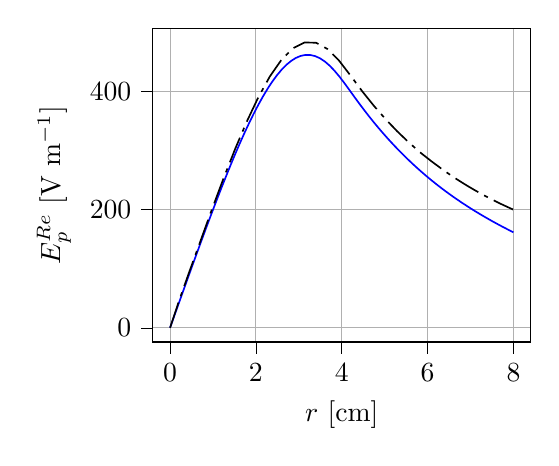
\begin{tikzpicture}

\definecolor{darkgray176}{RGB}{176,176,176}

\begin{axis}[
legend cell align=left,
legend pos= north east,
scale = .7,
ylabel = {$E_p^{Re}$ [V m$^{-1}$]},
xlabel = {$r$ [cm]},
tick align=outside,
tick pos=left,
x grid style={darkgray176},
xmajorgrids,
xmin=-0.399999991059303, xmax=8.39999981224537,
xtick style={color=black},
y grid style={darkgray176},
ymajorgrids,
ymin=-24.1311686001751, ymax=506.750031724057,
ytick style={color=black}
]
\addplot [semithick, blue]
table {%
0 -0.000204949073616048
0.007999999797903 1.62844558606776
0.015999999595806 3.25709612695349
0.023999999393709 4.88574667358378
0.031999999191612 6.51439722595879
0.039999998989515 8.14304778407872
0.047999998787418 9.77169834794376
0.0560000014957041 11.4003495100537
0.063999998383224 13.0289994929099
0.0720000010915101 14.657650666511
0.07999999797903 16.2863006608587
0.0880000006873161 17.9149518459517
0.095999997574836 19.5436018517916
0.104000000283122 21.1716173519445
0.112000002991408 22.7983363261801
0.119999994058162 24.4250529391082
0.127999996766448 26.0517719251028
0.135999999474734 27.6784909169771
0.14400000218302 29.3052099147313
0.151999993249774 30.9319265511788
0.15999999595806 32.5586455606934
0.167999998666346 34.1853645760886
0.176000001374632 35.8120835973645
0.183999992441386 37.4388002573343
0.191999995149672 39.0655192903721
0.199999986216426 40.6922359621042
0.208000000566244 42.3165126104302
0.215999991632998 43.9395138246715
0.224000005982816 45.5625197686372
0.23199999704957 47.1855209952065
0.239999988116324 48.80852222794
0.248000002466142 50.4315281903985
0.255999993532896 52.0545294354612
0.26399998459965 53.6775306866888
0.271999998949468 55.3005366676421
0.279999990016222 56.9235379312
0.28800000436604 58.546543924484
0.295999995432794 60.1695452003731
0.303999986499548 61.792546482428
0.312000000849366 63.4100018448072
0.31999999191612 65.0273793482368
0.327999982982874 66.6447568582475
0.335999997332692 68.2621390820328
0.343999988399446 69.8795166052063
0.352000002749264 71.4968988421548
0.359999993816018 73.1142763784919
0.367999984882772 74.731653921411
0.37599999923259 76.349036178106
0.383999990299344 77.96641373419
0.392000004649162 79.5837960040503
0.399999972432852 81.2011688661066
0.40799998678267 82.8161314148098
0.416000001132488 84.4258560571522
0.423999968916178 86.0355713368296
0.431999983265996 87.6452959934699
0.439999997615814 89.2550206572597
0.448000011965632 90.864745328199
0.455999979749322 92.4744606364741
0.46399999409914 94.0841853217132
0.472000008448958 95.6939100141026
0.479999976232648 97.3036253438284
0.487999990582466 98.913350050519
0.496000004932284 100.523074764361
0.503999972715974 102.132790115539
0.511999987065792 103.736182668301
0.52000000141561 105.336089911474
0.5279999691993 106.935987849826
0.535999983549118 108.535895108694
0.543999997898936 110.135802375411
0.551999965682626 111.735700337306
0.559999980032444 113.33560761972
0.567999994382262 114.935514909982
0.57600000873208 116.535422208093
0.58399997651577 118.135320201385
0.591999990865588 119.735227515195
0.600000005215406 121.335134836855
0.607999972999096 122.935032853696
0.615999987348914 124.52315259281
0.624000001698732 126.110957536334
0.631999969482422 127.698753246326
0.63999998383224 129.286558207234
0.647999998182058 130.874363176836
0.655999965965748 132.462158912906
0.663999980315566 134.049963899894
0.671999994665384 135.637768895575
0.679999962449074 137.225564657726
0.687999976798892 138.813369670796
0.69599999114871 140.401174692561
0.704000005498528 141.988979723021
0.711999973282218 143.572378258945
0.719999987632036 145.145670324856
0.728000001981854 146.718962400452
0.735999969765544 148.292245327986
0.743999984115362 149.865537422955
0.75199999846518 151.438829527611
0.75999996624887 153.012112484206
0.767999980598688 154.585404608237
0.775999994948506 156.158696741956
0.784000009298325 157.731988885363
0.791999977082014 159.305271880709
0.799999944865704 160.878554885744
0.808000005781651 162.451856215967
0.81599997356534 164.014364495718
0.82399994134903 165.570598675273
0.832000002264977 167.126850982672
0.839999970048666 168.683085183869
0.847999937832355 170.239319395887
0.855999998748302 171.795571735751
0.863999966531992 173.351805969413
0.871999934315681 174.908040213897
0.879999995231628 176.464292586229
0.887999963015318 178.020526852359
0.896000023931265 179.576779246338
0.903999991714954 181.133013534116
0.911999959498644 182.689247832718
0.920000020414591 184.226558146699
0.92799998819828 185.763081680709
0.93599995598197 187.299605226835
0.944000016897917 188.836146672637
0.951999984681606 190.372670242997
0.959999952465296 191.909193825473
0.968000013381243 193.445735307629
0.975999981164932 194.982258914341
0.983999948948622 196.518782533172
0.992000009864569 198.055324051683
0.999999977648258 199.591847694753
1.00799994543195 201.128371349941
1.01600000634789 202.657878199007
1.02399997413158 204.171126048392
1.03199994191527 205.684373957913
1.04000000283122 207.197639544157
1.04799997061491 208.71088757392
1.0559999383986 210.224135663845
1.06399999931455 211.737401430347
1.07199996709824 213.25064964041
1.07999993488193 214.76389791062
1.08799999579787 216.277163857272
1.09599996358156 217.790412247494
1.10399993136525 219.303660697753
1.1119999922812 220.816926824642
1.11999996006489 222.323379520609
1.12800002098083 223.809778151595
1.13599998876452 225.29615954818
1.14399995654821 226.782541014174
1.15200001746416 228.268939853396
1.15999998524785 229.755321458234
1.16799995303154 231.241703132328
1.17600001394749 232.728102179687
1.18399998173118 234.214483992638
1.19199994951487 235.700865874716
1.20000001043081 237.187265130063
1.2079999782145 238.673647150887
1.21599994599819 240.160029241006
1.22400000691414 241.639827130725
1.23199997469783 243.09563400868
1.23999994248152 244.55144096664
1.24800000339746 246.007264952484
1.25599997118115 247.46307207041
1.26399993896484 248.91887926836
1.27199999988079 250.37470349403
1.27999996766448 251.83051085181
1.28799993544817 253.28631828958
1.29599999636412 254.742142754957
1.30399996414781 256.19795035243
1.3119999319315 257.653758029775
1.31999999284744 259.10958273488
1.32799996063113 260.55921113774
1.33599992841482 261.980474915683
1.34399998933077 263.40175533127
1.35199995711446 264.823019292976
1.35999992489815 266.244283346537
1.36799998581409 267.665564037761
1.37599995359778 269.086828274925
1.38400001451373 270.508109149727
1.39199998229742 271.929373570629
1.39999995008111 273.350638083121
1.40800001099706 274.771919233232
1.41599997878075 276.193183929317
1.42399994656444 277.614448717124
1.43200000748038 279.03022868034
1.43999997526407 280.412719854762
1.44799994304776 281.795211134276
1.45600000396371 283.177718613246
1.4639999717474 284.560210102887
1.47199993953109 285.942701697628
1.48000000044703 287.325209491644
1.48799996823072 288.707701296339
1.49599993601441 290.09019320608
1.50399999693036 291.472701314999
1.51199996471405 292.855193434558
1.51999993249774 294.237685659036
1.52799999341369 295.620194082808
1.53599996119738 296.99814858386
1.54399992898107 298.33737731272
1.55199998989701 299.67662175191
1.5599999576807 301.015850719931
1.56800001859665 302.35509539824
1.57599989324808 303.694309014658
1.58399995416403 305.033553931937
1.59200001507998 306.372798968767
1.59999988973141 307.71201294363
1.60799995064735 309.05125821927
1.6160000115633 310.390503614413
1.62399988621473 311.729717947448
1.63199994713068 313.06896358136
1.64000000804663 314.404948060599
1.64799988269806 315.696148360063
1.65599994361401 316.987378858522
1.66400000452995 318.27860949238
1.67199987918139 319.569810198033
1.67999994009733 320.861041102683
1.68800000101328 322.152272142531
1.69599987566471 323.443473254153
1.70399993658066 324.734704564704
1.7119999974966 326.025936010363
1.71999987214804 327.317137527726
1.72799993306398 328.60836924389
1.73599999397993 329.899601095231
1.74399986863136 331.189162021284
1.75199992954731 332.427366820197
1.75999999046326 333.665571771662
1.7680000513792 334.903776875651
1.77599992603064 336.14195330314
1.78399998694658 337.380158712157
1.79200004786253 338.618364273485
1.79999992251396 339.856541158282
1.80799998342991 341.094747024527
1.81600004434586 342.332953042996
1.82399991899729 343.571130384849
1.83199997991323 344.809336708015
1.84000004082918 346.047543183455
1.84799991548061 347.285720982114
1.85599997639656 348.465977096911
1.86400003731251 349.645884170859
1.87199991196394 350.825763944206
1.87999997287989 352.005671360214
1.88800003379583 353.185578947274
1.89599990844727 354.3654592335
1.90399996936321 355.545367162363
1.91200003027916 356.725275262176
1.91999990493059 357.905156061056
1.92799996584654 359.085064502498
1.93600002676249 360.264973114738
1.94399990141392 361.444854426059
1.95199996232986 362.624763379797
1.96000002324581 363.743578441157
1.96799989789724 364.859628590711
1.97599995881319 365.975704916619
1.98400001972914 367.091781433373
1.99199989438057 368.207832155516
1.99999995529652 369.323909053798
2.00800001621246 370.439986142876
2.0159998908639 371.556037437214
2.02399995177984 372.672114907616
2.03200001269579 373.788192568713
2.03999988734722 374.904244434897
2.04799994826317 376.020322477162
2.05600000917912 377.136400709961
2.06399988383055 378.18882824399
2.07199994474649 379.233549090988
2.08000000566244 380.278269410468
2.08799988031387 381.322964878796
2.09599994122982 382.367684144608
2.10400000214577 383.412402884255
2.1119998767972 384.457096774144
2.11999993771315 385.501814462814
2.12799999862909 386.546531626674
2.13599987328053 387.591223942151
2.14399993419647 388.635940057732
2.15199999511242 389.680655649837
2.15999986976385 390.725346394938
2.1679999306798 391.747444078118
2.17599999159575 392.71396832902
2.18399986624718 393.680469471959
2.19199992716312 394.646992514373
2.19999998807907 395.613514953308
2.2079998627305 396.580014285867
2.21599992364645 397.546535519563
2.2239999845624 398.513056151127
2.23199985921383 399.479553677792
2.23999992012978 400.446073107059
2.24799998104572 401.412591935922
2.25600004196167 402.379110164891
2.2639999166131 403.345605291163
2.27199997752905 404.312122321888
2.280000038445 405.222597531742
2.28799991309643 406.103957021769
2.29599997401237 406.985336345733
2.30400003492832 407.866714983136
2.31199990957975 408.748072413548
2.3199999704957 409.629449679595
2.32800003141165 410.510826260841
2.33599990606308 411.39218163686
2.34399996697903 412.273556850223
2.35200002789497 413.15493138051
2.35999990254641 414.036284707383
2.36799996346235 414.917657873273
2.3760000243783 415.799030357822
2.38399989902973 416.677893792129
2.39199995994568 417.467604095829
2.40000002086163 418.25731362485
2.40799989551306 419.047003993157
2.415999956429 419.836711974802
2.42400001734495 420.626419183731
2.43199989199638 421.41610723396
2.43999995291233 422.205812899453
2.44800001382828 422.995517794144
2.45599988847971 423.785203532164
2.46399994939566 424.574906887325
2.4720000103116 425.364609473675
2.47999988496304 426.154292905335
2.48799994587898 426.943993956027
2.49600000679493 427.694983260641
2.50399988144636 428.386901492366
2.51199994236231 429.078834970648
2.52000000327826 429.770767585973
2.52799987792969 430.46268322891
2.53599993884563 431.154614120524
2.54399999976158 431.84654415143
2.55199987441301 432.538457212178
2.55999993532896 433.23038552351
2.56799999624491 433.922312976372
2.57599987089634 434.614223461309
2.58399993181229 435.306149199139
2.59199999272823 435.998074080523
2.59999986737967 436.689981996203
2.60799992829561 437.30280232044
2.61599998921156 437.891276268538
2.62399986386299 438.479735562259
2.63199992477894 439.068207605103
2.63999998569489 439.656678696507
2.64799986034632 440.245135135997
2.65599992126226 440.833604326938
2.66399998217821 441.422072568827
2.67199985682964 442.010526161257
2.67999991774559 442.598992507456
2.68799997866154 443.187457906989
2.69599985331297 443.775908659506
2.70399991422892 444.364372168104
2.71199997514486 444.938344077867
2.7199998497963 445.418084015662
2.72799991071224 445.897834081986
2.73599997162819 446.377583107704
2.74399984627962 446.857319923782
2.75199990719557 447.337066870924
2.75999996811152 447.816812780194
2.76800002902746 448.296557652106
2.77599990367889 448.776290318014
2.78399996459484 449.256033118382
2.79200002551079 449.735774884212
2.79999990016222 450.21550444663
2.80799996107817 450.695244145996
2.81600002199411 451.17498281341
2.82399989664555 451.597726939942
2.83199995756149 451.963911844466
2.84000001847744 452.330095623123
2.84799989312887 452.696269751075
2.85599995404482 453.062451280836
2.86400001496077 453.42863168754
2.8719998896122 453.794802446443
2.87999995052814 454.160980609934
2.88800001144409 454.527157653
2.89599988609552 454.893325051214
2.90399994701147 455.259499856677
2.91200000792742 455.625673544673
2.91999988257885 455.991837590589
2.9279999434948 456.35800904646
2.93600000441074 456.621511080147
2.94399987906218 456.869702625263
2.95199993997812 457.117898744246
2.96000000089407 457.36609365933
2.9679998755455 457.614281592862
2.97599993646145 457.86247410317
2.9839999973774 458.110665412571
2.99199987202883 458.358849743491
2.99999993294477 458.607038654089
3.00799999386072 458.855226366761
3.01599986851215 459.103407104015
3.0239999294281 459.351592423837
3.03199999034405 459.599776548705
3.03999986499548 459.818848256624
3.04799992591143 459.94505916511
3.05599998682737 460.071268795237
3.06399986147881 460.197474209582
3.07199992239475 460.32368128619
3.0799999833107 460.449887087606
3.08799985796213 460.576088676507
3.09599991887808 460.702291930718
3.10399997979403 460.82849391289
3.11199985444546 460.954691685782
3.1199999153614 461.080891127065
3.12799997627735 461.207089299456
3.1360000371933 461.333286204002
3.14400009810925 461.459481841746
3.15199978649616 461.519248207492
3.15999984741211 461.51897015267
3.16799990832806 461.518692327314
3.175999969244 461.518414730702
3.18400003015995 461.518137362117
3.1920000910759 461.517860220841
3.19999977946281 461.517583319053
3.20799984037876 461.517306630252
3.21599990129471 461.517030166633
3.22399996221066 461.516753927492
3.2320000231266 461.516477912127
3.24000008404255 461.516202119841
3.24799977242947 461.515926562766
3.25599983334541 461.515651214546
3.26399989426136 461.477164105386
3.27199995517731 461.348964947294
3.28000001609325 461.220766004232
3.2880000770092 461.092567275533
3.29599976539612 460.964374730191
3.30399982631207 460.83617642822
3.31199988722801 460.70797833863
3.31999994814396 460.579780460768
3.32800000905991 460.451582793969
3.33600006997585 460.323385337597
3.34399975836277 460.195194060598
3.35199981927872 460.06699702312
3.35999988019466 459.938800194129
3.36799994111061 459.810603572986
3.37600000202656 459.682407159053
3.3840000629425 459.425967736592
3.39199975132942 459.168311287793
3.39999981224537 458.910643033879
3.40799987316132 458.652974972793
3.41599993407726 458.395307103949
3.42399999499321 458.13763942676
3.43200005590916 457.87997194064
3.43999974429607 457.62231664349
3.44799980521202 457.364649537769
3.45599986612797 457.106982621386
3.46399992704391 456.849315893765
3.47199998795986 456.591649354336
3.48000004887581 456.33398300253
3.48799973726273 456.076328836199
3.49599979817867 455.732542105097
3.50399985909462 455.348643435229
3.51199992001057 454.964744932318
3.51999998092651 454.58084659586
3.52800004184246 454.196948425355
3.53600010275841 453.813050420306
3.54399979114532 453.42917045671
3.55199985206127 453.045272781075
3.55999991297722 452.661375269411
3.56799997389317 452.277477921229
3.57600003480911 451.893580736039
3.58400009572506 451.509683713354
3.59199978411198 451.125804729142
3.59999984502792 450.741908030011
3.60799990594387 450.313803173328
3.61599996685982 449.811701288585
3.62400002777576 449.309599540463
3.63200008869171 448.807497928559
3.63999977707863 448.305419833209
3.64799983799458 447.803318492522
3.65599989891052 447.301217286845
3.66399995982647 446.79911621578
3.67200002074242 446.297015278928
3.68000008165836 445.794914475893
3.68799977004528 445.292837186986
3.69599983096123 444.790736650399
3.70399989187717 444.288636246451
3.71199995279312 443.786535974753
3.72000001370907 443.277507983114
3.72800007462502 442.670017612046
3.73599976301193 442.062555632511
3.74399982392788 441.455065467696
3.75199988484383 440.847575405556
3.75999994575977 440.240085445793
3.76800000667572 439.632595588107
3.77600006759167 439.025105832194
3.78399975597858 438.417644466002
3.79199981689453 437.810154912762
3.79999987781048 437.202665460416
3.80799993872643 436.595176108671
3.81599999964237 435.987686857234
3.82400006055832 435.380197705816
3.83199974894524 434.772736942322
3.83999980986118 434.098756903845
3.84799987077713 433.403480630189
3.85599993169308 432.70820442457
3.86399999260902 432.012928286791
3.87200005352497 431.317652216656
3.87999974191189 430.622408590036
3.88799980282784 429.927132654604
3.89599986374378 429.231856786235
3.90399992465973 428.536580984736
3.91199998557568 427.841305249916
3.92000004649162 427.146029581583
3.92799973487854 426.450786355592
3.93599979579449 425.75551081966
3.94399985671043 425.060235349646
3.95199991762638 424.335589299325
3.95999997854233 423.574917235826
3.96800003945827 422.814245204492
3.97599972784519 422.053608626512
3.98399978876114 421.292936659233
3.99199984967709 420.532264723845
3.99999991059303 419.771592820259
4.00799997150898 419.010920948383
4.01600003242493 418.250249108129
4.02400009334087 417.489577299406
4.03199978172779 416.728940943395
4.03999984264374 415.968269197466
4.04799990355968 415.207597482803
4.05599996447563 414.446925799317
4.06400002539158 413.680872883382
4.07200008630753 412.881983273484
4.07999977469444 412.083130860822
4.08799983561039 411.28424124358
4.09599989652634 410.48535162268
4.10399995744228 409.686461998133
4.11200001835823 408.887572369949
4.12000007927418 408.088682738139
4.12799976766109 407.289830303627
4.13599982857704 406.490940664594
4.14399988949299 405.692051021965
4.15199995040894 404.893161375749
4.16000001132488 404.094271725958
4.16800007224083 403.2953820726
4.17599976062775 402.496529616601
4.18399982154369 401.692435907757
4.19199988245964 400.887294580091
4.19999994337559 400.082153213793
4.20800000429153 399.27701180897
4.21600006520748 398.471870365728
4.2239997535944 397.666766376211
4.23199981451035 396.861624856452
4.23999987542629 396.056483298592
4.24799993634224 395.251341702736
4.25599999725819 394.446200068988
4.26400005817413 393.641058397454
4.27199974656105 392.835954180284
4.279999807477 392.030812433489
4.28799986839294 391.225670649217
4.29599992930889 390.419431078188
4.30399999022484 389.624714248297
4.31200005114079 388.829997649314
4.3199997395277 388.035318288454
4.32799980044365 387.240602153189
4.3359998613596 386.445886250751
4.34399992227554 385.651170581783
4.35199998319149 384.856455146931
4.36000004410744 384.061739946844
4.36799973249435 383.267061988686
4.3759997934103 382.472347260074
4.38399985432625 381.677632768189
4.3919999152422 380.882918513687
4.39999997615814 380.088204497231
4.40800003707409 379.301608371988
4.41599972546101 378.529875613488
4.42399978637695 377.758107146899
4.4319998472929 376.986338910874
4.43999990820885 376.214570906059
4.44799996912479 375.442803133101
4.45600003004074 374.67103559265
4.46399971842766 373.899304223294
4.47199977934361 373.127537149804
4.47999984025955 372.355770310784
4.4879999011755 371.584003706894
4.49599996209145 370.812237338795
4.50400002300739 370.040471207153
4.51200008392334 369.268705312634
4.51999977231026 368.501322637029
4.5279998332262 367.753242073412
4.53599989414215 367.005161732856
4.5439999550581 366.257081615993
4.55200001597404 365.509001723455
4.56000007688999 364.76092205588
4.56799976527691 364.012877448799
4.57599982619286 363.264798233091
4.5839998871088 362.516719244201
4.59199994802475 361.768640482877
4.6000000089407 361.020561949734
4.60800006985664 360.272483645422
4.61599975824356 359.524440405425
4.62399981915951 358.776362560728
4.63199988007545 358.028284946831
4.6399999409914 357.304626269648
4.64800000190735 356.580644311909
4.6560000628233 355.856662566127
4.66399975121021 355.132714745665
4.67199981212616 354.408733425614
4.67999987304211 353.684752319352
4.68799993395805 352.960771427514
4.695999994874 352.236790750664
4.70400005578995 351.512810289475
4.71199974417686 350.788863757249
4.71999980509281 350.06488372921
4.72799986600876 349.34090391869
4.73599992692471 348.616924326321
4.74399998784065 347.892944952734
4.7520000487566 347.189356115678
4.75999973714352 346.489585689551
4.76799979805946 345.789782873063
4.77599985897541 345.08998025366
4.78399991989136 344.390177831917
4.7919999808073 343.690375608409
4.80000004172325 342.990573583716
4.80799973011017 342.290804345227
4.81599979102612 341.591002719899
4.82399985194206 340.891201295136
4.83199991285801 340.191400071524
4.83999997377396 339.491599049655
4.8480000346899 338.791798230121
4.85599972307682 338.092030200269
4.86399978399277 337.408343672546
4.87199984490871 336.732470519187
4.87999990582466 336.056597544488
4.88799996674061 335.380724748975
4.89600002765656 334.704852133179
4.90399971604347 334.029011170149
4.91199977695942 333.353138915373
4.91999983787537 332.677266841914
4.92799989879131 332.001394950309
4.93599995970726 331.325523241098
4.94400002062321 330.649651714824
4.95199970901012 329.973811844498
4.95999976992607 329.297940685723
4.96799983084202 328.622069711523
4.97599989175797 327.957958622593
4.98399995267391 327.30543662841
4.99200001358986 326.652914794151
4.99999970197678 326.000423505466
5.00799976289272 325.347901992484
5.01599982380867 324.695380640866
5.02399988472462 324.042859451098
5.03199994564056 323.390338423665
5.04000000655651 322.737817559055
5.04800006747246 322.08529685776
5.05599975585938 321.43280670539
5.06399981677532 320.780286332193
5.07199987769127 320.127766123792
5.07999993860722 319.475246080686
5.08799999952316 318.830220665213
5.09600006043911 318.200141591037
5.10399974882603 317.570091998897
5.11199980974197 316.940013208995
5.11999987065792 316.309934561881
5.12799993157387 315.67985605799
5.13599999248981 315.049777697757
5.14400005340576 314.419699481619
5.15199974179268 313.789650750088
5.15999980270863 313.159572823456
5.16799986362457 312.529495042244
5.17599992454052 311.899417406897
5.18399998545647 311.269339917862
5.19200004637241 310.639262575586
5.19999973475933 310.012699455125
5.20799979567528 309.403825562394
5.21599985659122 308.79495179622
5.22399991750717 308.186078156992
5.23199997842312 307.577204645101
5.24000003933907 306.968331260941
5.24799972772598 306.359486357556
5.25599978864193 305.750613230057
5.26399984955788 305.141740231432
5.27199991047382 304.532867362147
5.27999997138977 303.92399462258
5.28800003230572 303.315122013135
5.29599972069263 302.70627788683
5.30399978160858 302.097405538836
5.31199984252453 301.488533322181
5.31999990344048 300.899197297156
5.32799996435642 300.309961528538
5.33600002527237 299.720725876215
5.34399971365929 299.131517778757
5.35199977457523 298.54228236011
5.35999983549118 297.953047058853
5.36799989640713 297.363811875382
5.37599995732307 296.774576809984
5.38400001823902 296.185341863112
5.39199970662594 295.596134473286
5.39999976754189 295.006899764527
5.40799982845783 294.417665175391
5.41599988937378 293.828430706255
5.42399995028973 293.239196357498
5.43200001120567 292.667678202716
5.43999969959259 292.098106879121
5.44799976050854 291.528509019084
5.45599982142448 290.958911146356
5.46399988234043 290.389313260928
5.47199994325638 289.819715362787
5.48000000417233 289.25011745193
5.48799969255924 288.680546052092
5.49599975347519 288.110948115748
5.50399981439114 287.541350166647
5.51199987530708 286.971752204777
5.51999993622303 286.402154230127
5.52799999713898 285.832556242686
5.53600005805492 285.273020894278
5.54399974644184 284.721062988077
5.55199980735779 284.169079365457
5.55999986827374 283.617095729952
5.56799992918968 283.06511208155
5.57599999010563 282.513128420238
5.58400005102158 281.961144746007
5.59199973940849 281.409186762392
5.59999980032444 280.857203062286
5.60799986124039 280.305219349226
5.61599992215633 279.7532356232
5.62399998307228 279.201251884196
5.63200004398823 278.649268132204
5.63999973237514 278.102771652316
5.64799979329109 277.568020575933
5.65599985420704 277.033269486498
5.66399991512299 276.498518383999
5.67199997603893 275.963767268425
5.68000003695488 275.429016139765
5.6879997253418 274.894289899126
5.69599978625774 274.35953874433
5.70399984717369 273.824787576252
5.71199990808964 273.290036395129
5.71999996900558 272.755285200862
5.72800002992153 272.220533993438
5.73599971830845 271.68580767395
5.7439997792244 271.152109290448
5.75199984014034 270.634165787755
5.75999990105629 270.116222271852
5.76799996197224 269.598278742727
5.77600002288818 269.080335200368
5.7839997112751 268.562415763207
5.79199977219105 268.044472194404
5.79999983310699 267.52652861225
5.80799989402294 267.008585016804
5.81599995493889 266.4906414081
5.82400001585484 265.972697786091
5.83199970424175 265.454778269211
5.8399997651577 264.936834620557
5.84799982607365 264.418890958563
5.85599988698959 263.914155587696
5.86399994790554 263.412551583048
5.87200000882149 262.910947565029
5.8799996972084 262.409366891209
5.88799975812435 261.907762846414
5.8959998190403 261.406158788214
5.90399987995625 260.9045547166
5.91199994087219 260.402950631545
5.92000000178814 259.901346533053
5.92799969017506 259.39976577869
5.935999751091 258.898161653277
5.94399981200695 258.396557514386
5.9519998729229 257.894953362004
5.95999993383884 257.402119577409
5.96799999475479 256.916344056329
5.97599968314171 256.430591142246
5.98399974405766 255.94481559412
5.9919998049736 255.459040032452
5.99999986588955 254.97326445723
6.0079999268055 254.487488868443
6.01599998772144 254.001713266075
6.02400004863739 253.515937650118
6.03199973702431 253.030184641076
6.03999979794025 252.544408997902
6.0479998588562 252.058633341099
6.05599991977215 251.572857670657
6.0639999806881 251.091661441494
6.07200004160404 250.621160089421
6.07999972999096 250.150680632944
6.08799979090691 249.680179253531
6.09599985182285 249.209677860429
6.1039999127388 248.739176453626
6.11199997365475 248.268675033129
6.12000003457069 247.798173598946
6.12799972295761 247.327694060154
6.13599978387356 246.857192598425
6.14399984478951 246.386691122933
6.15199990570545 245.916189633665
6.1599999666214 245.445688130609
6.16800002753735 244.975855201705
6.17599971592426 244.520051999758
6.18399977684021 244.064227558172
6.19199983775616 243.608403102751
6.1999998986721 243.152578633483
6.20799995958805 242.696754150356
6.216000020504 242.240929653412
6.22399970889091 241.785126368322
6.23199976980686 241.329301843511
6.23999983072281 240.87347730482
6.24799989163876 240.417652752205
6.2559999525547 239.961828185655
6.26399964094162 239.506024830982
6.2720000743866 239.050179010698
6.27999976277351 238.60548210759
6.28800019621849 238.163673495224
6.29599988460541 237.721906013253
6.30399957299232 237.280138517263
6.3120000064373 236.838329862831
6.31999969482422 236.39656233876
6.3280001282692 235.954753656224
6.33599981665611 235.512986104017
6.34399950504303 235.071218537731
6.35199993848801 234.629409812932
6.35999962687492 234.187642218437
6.3680000603199 233.745833465402
6.37599974870682 233.304065842647
6.38400018215179 232.86942840471
6.39199987053871 232.441013256057
6.39999955892563 232.012598093199
6.40799999237061 231.584143015294
6.41599968075752 231.155727823985
6.4240001142025 230.7272727176
6.43199980258942 230.298857497788
6.43999949097633 229.870442263703
6.44799992442131 229.441987114501
6.45599961280823 229.013571851835
6.4640000462532 228.585116674022
6.47199973464012 228.156701382722
6.4800001680851 227.728246176246
6.48799985647202 227.303370470229
6.49599954485893 226.887387054178
6.50399997830391 226.471364758779
6.51199966669083 226.055381070027
6.5200001001358 225.639358501827
6.52799978852272 225.223374540241
6.5360002219677 224.807351699182
6.54399991035461 224.391367464723
6.55199959874153 223.975383093804
6.56000003218651 223.559359843312
6.56799972057343 223.143375199364
6.5760001540184 222.727351675793
6.58399984240532 222.311366758783
6.59199953079224 221.902395069869
6.59999996423721 221.4979764362
6.60799965262413 221.093595331383
6.61600008606911 220.689176430631
6.62399977445602 220.28479505869
6.632000207901 219.880375890737
6.63999989628792 219.475994251612
6.64799958467484 219.071612478873
6.65600001811981 218.667192910027
6.66399970650673 218.262810869987
6.67200013995171 217.858391033736
6.67999982833862 217.454008726297
6.68799951672554 217.049626285141
6.69599995017052 216.655485136171
6.70399963855743 216.262201830974
6.71200007200241 215.868881766209
6.71999976038933 215.475598199395
6.7280001938343 215.082277872928
6.73599988222122 214.688994044441
6.74399957060814 214.295710085096
6.75200000405312 213.902389366005
6.75999969244003 213.509105144872
6.76800012588501 213.115784163932
6.77599981427193 212.722499680889
6.78399950265884 212.329215066917
6.79199993610382 211.93852423894
6.79999962449074 211.555857756358
6.80800005793571 211.173155505723
6.81599974632263 210.790488767024
6.82400017976761 210.407786260179
6.83199986815453 210.025119265239
6.83999955654144 209.642452142175
6.84799998998642 209.259749250909
6.85599967837334 208.877081871529
6.86400011181831 208.494378723885
6.87199980020523 208.11171108808
6.87999948859215 207.729043324071
6.88799992203712 207.346339791703
6.89599961042404 206.96945761749
6.90400004386902 206.596916122653
6.91199973225594 206.224409196139
6.92000016570091 205.851867450422
6.92799985408783 205.47936027299
6.93599954247475 205.106852970086
6.94399997591972 204.734310847876
6.95199966430664 204.361803293962
6.96000009775162 203.989260920682
6.96799978613853 203.616753115683
6.97599947452545 203.244245185084
6.98399990797043 202.871702435047
6.99199959635735 202.499194253266
7.00000002980232 202.135320622227
7.00799971818924 201.772540234456
7.01600015163422 201.409725935994
7.02399984002113 201.046945302532
7.03199952840805 200.684164546215
7.03999996185303 200.321349879099
7.04799965023994 199.958568877003
7.05600008368492 199.595753964051
7.06399977207184 199.232972716106
7.07200020551682 198.870157557245
7.07999989390373 198.507376063336
7.08799958229065 198.144594446467
7.09600001573563 197.783762631615
7.10399970412254 197.430299390806
7.11200013756752 197.076803109598
7.11999982595444 196.72333962824
7.12799951434135 196.369876026547
7.13599994778633 196.016379384374
7.14399963617325 195.662915542016
7.15200006961823 195.309418659119
7.15999975800514 194.955954576025
7.16800019145012 194.602457452335
7.17599987983704 194.248993128404
7.18399956822395 193.895528684062
7.19200000166893 193.542031199033
7.19999969005585 193.19334213038
7.20800012350082 192.848778299481
7.21599981188774 192.504246439044
7.22399950027466 192.159714460803
7.23199993371964 191.815150276396
7.23999962210655 191.470618062436
7.24800005555153 191.12605364228
7.25599974393845 190.781521192559
7.26400017738342 190.436956536586
7.27199986577034 190.092423851034
7.27999955415726 189.747891047514
7.28799998760223 189.403326037672
7.29599967598915 189.05879299823
7.30400010943413 188.721568577439
7.31199979782104 188.385606646724
7.31999948620796 188.049644600637
7.32799991965294 187.713651148967
7.33599960803986 187.377688871999
7.34400004148483 187.04169518943
7.35199972987175 186.705732681552
7.36000016331673 186.369738768017
7.36799985170364 186.033776029161
7.37599954009056 185.697813174796
7.38399997353554 185.361818914653
7.39199966192245 185.025855829189
7.40000009536743 184.691328576676
7.40799978375435 184.363598740373
7.41599947214127 184.035868791048
7.42399990558624 183.708108205268
7.43199959397316 183.38037802983
7.44000002741814 183.052617217868
7.44799971580505 182.724886816267
7.45600014925003 182.397125778088
7.46399983763695 182.069395150258
7.47199952602386 181.741664409294
7.47999995946884 181.413903031644
7.48799964785576 181.086172064335
7.49600008130074 180.75841046031
7.50399976968765 180.432999209561
7.51200020313263 180.109886204831
7.51999989151955 179.787340380321
7.52799957990646 179.465546474288
7.53600001335144 179.144149614349
7.54399970173836 178.823636700363
7.55200013518333 178.503412076721
7.55999982357025 178.184171593558
7.56799951195717 177.865141691915
7.57599994540215 177.547135499421
7.58399963378906 177.229263534635
7.59200006723404 176.912513446006
7.59999975562096 176.595792855429
7.60800018906593 176.280290374543
7.61599987745285 175.964817313631
7.62399956583977 175.650480078743
7.63199999928474 175.336216859967
7.63999968767166 175.023008972675
7.64800012111664 174.709977155716
7.65599980950356 174.397891697584
7.66399949789047 174.086111966326
7.67199993133545 173.77511261831
7.67999961972237 173.464547117926
7.68800005316734 173.154657509353
7.69599974155426 172.845300204312
7.70400017499924 172.53651423346
7.71199986338615 172.228357122068
7.71999955177307 171.920696736407
7.72799998521805 171.613703292403
7.73599967360497 171.307133383856
7.74400010704994 171.001324985655
7.75199979543686 170.695839328933
7.75999948382378 170.391236533951
7.76799991726875 170.086800260828
7.77599960565567 169.783366843645
7.78400003910065 169.480002029237
7.79199972748756 169.177730852594
7.80000016093254 168.875431523657
7.80799984931946 168.574314989911
7.81599953770638 168.273198432938
7.82399997115135 167.973105342722
7.83199965953827 167.67313584957
7.84000009298325 167.374088554641
7.84799978137016 167.075259188504
7.85599946975708 166.777279495769
7.86399990320206 166.479555357278
7.87199959158897 166.182609327775
7.88000002503395 165.886010911331
7.88799971342087 165.590092781148
7.89600014686584 165.294613347318
7.90399983525276 164.999717264252
7.91199952363968 164.705377017259
7.91999995708466 164.411469587708
7.92799964547157 164.11823386761
7.93600007891655 163.825336854266
7.94399976730347 163.533199110099
7.95199945569038 163.241334042629
7.95999988913536 162.950260152773
7.96799957752228 162.659393987872
7.97600001096725 162.369404211274
7.98399969935417 162.079531208171
7.99200013279915 161.790619181234
7.99999982118607 161.501734059869
};
\addplot [semithick, black, dash pattern=on 9.6pt off 2.4pt on 1.5pt off 2.4pt]
table {%
0 0
0.00800800800800801 1.75144175782191
0.016016016016016 3.50288351564383
0.024024024024024 5.25432527346574
0.032032032032032 7.00511494751343
0.04004004004004 8.75554021648261
0.048048048048048 10.5059654854518
0.0560560560560561 12.256390754421
0.0640640640640641 14.0068160233902
0.0720720720720721 15.7572412923593
0.0800800800800801 17.5076665613285
0.0880880880880881 19.2580918302977
0.0960960960960961 21.0085170992669
0.104104104104104 22.7589423682361
0.112112112112112 24.5093676372053
0.12012012012012 26.2597929061744
0.128128128128128 28.0102181751436
0.136136136136136 29.7606434441128
0.144144144144144 31.511068713082
0.152152152152152 33.2614939820512
0.16016016016016 35.0119192510204
0.168168168168168 36.7623445199895
0.176176176176176 38.5131596050527
0.184184184184184 40.2646013628747
0.192192192192192 42.0160431206966
0.2002002002002 43.7648479687667
0.208208208208208 45.4108083314303
0.216216216216216 47.0567686940938
0.224224224224224 48.7027290567574
0.232232232232232 50.348689419421
0.24024024024024 51.9935486700744
0.248248248248248 53.638402172242
0.256256256256256 55.2832556744096
0.264264264264264 56.9281091765772
0.272272272272272 58.5729626787448
0.28028028028028 60.2178161809124
0.288288288288288 61.8626696830799
0.296296296296296 63.5075231852475
0.304304304304304 65.1523766874152
0.312312312312312 66.7972301895827
0.32032032032032 68.4420836917503
0.328328328328328 70.0869371939179
0.336336336336336 71.7317906960855
0.344344344344344 73.3766441982531
0.352352352352352 75.0214977004207
0.36036036036036 76.6663512025883
0.368368368368368 78.3112047047559
0.376376376376376 79.9560582069235
0.384384384384384 81.6009117090911
0.392392392392392 83.2457652112587
0.4004004004004 84.8906187134263
0.408408408408408 86.5355665119359
0.416416416416416 88.1815268745995
0.424424424424424 89.827487237263
0.432432432432432 91.4734475999266
0.44044044044044 93.1170690631789
0.448448448448448 94.7205042121977
0.456456456456456 96.3239393612165
0.464464464464464 97.9273745102354
0.472472472472473 99.5308096592542
0.48048048048048 101.133468042587
0.488488488488488 102.73545333224
0.496496496496497 104.337438621893
0.504504504504504 105.939423911546
0.512512512512513 107.541409201199
0.520520520520521 109.143394490851
0.528528528528528 110.745379780504
0.536536536536537 112.347365070157
0.544544544544545 113.94935035981
0.552552552552553 115.551335649462
0.560560560560561 117.153320939115
0.568568568568569 118.755306228768
0.576576576576577 120.357291518421
0.584584584584585 121.959276808073
0.592592592592593 123.561262097726
0.600600600600601 125.163247387379
0.608608608608609 126.765232677032
0.616616616616617 128.367217966684
0.624624624624625 129.969203256337
0.632632632632633 131.57118854599
0.640640640640641 133.173173835643
0.648648648648649 134.775159125296
0.656656656656657 136.377144414948
0.664664664664665 137.979129704601
0.672672672672673 139.581114994254
0.680680680680681 141.184502953253
0.688688688688689 142.787938102272
0.696696696696697 144.39137325129
0.704704704704705 145.994808400309
0.712712712712713 147.600745047586
0.720720720720721 149.209761354921
0.728728728728729 150.818777662255
0.736736736736737 152.42779396959
0.744744744744745 154.036810276925
0.752752752752753 155.643874998096
0.760760760760761 157.25079046795
0.768768768768769 158.857705937804
0.776776776776777 160.464621407657
0.784784784784785 162.071536877511
0.792792792792793 163.678452347364
0.800800800800801 165.285367817218
0.808808808808809 166.892283287072
0.816816816816817 168.499198756925
0.824824824824825 170.106114226779
0.832832832832833 171.713029696632
0.840840840840841 173.319945166486
0.848848848848849 174.92686063634
0.856856856856857 176.533776106193
0.864864864864865 178.140691576047
0.872872872872873 179.7476070459
0.880880880880881 181.354522515754
0.888888888888889 182.961437985608
0.896896896896897 184.568353455461
0.904904904904905 186.175268925315
0.912912912912913 187.782184395168
0.920920920920921 189.389099865022
0.928928928928929 190.996015334876
0.936936936936937 192.602930804729
0.944944944944945 194.210603953896
0.952952952952953 195.819620261231
0.960960960960961 197.428636568566
0.968968968968969 199.0376528759
0.976976976976977 200.646669183235
0.984984984984985 202.209498446839
0.992992992992993 203.763622187414
1.001001001001 205.317745927989
1.00900900900901 206.871869668564
1.01701701701702 208.425041168197
1.02502502502503 209.976209115738
1.03303303303303 211.527377063279
1.04104104104104 213.07854501082
1.04904904904905 214.62971295836
1.05705705705706 216.180880905901
1.06506506506507 217.732048853442
1.07307307307307 219.283216800983
1.08108108108108 220.834384748524
1.08908908908909 222.385552696065
1.0970970970971 223.936720643606
1.10510510510511 225.487888591147
1.11311311311311 227.039056538688
1.12112112112112 228.590224486229
1.12912912912913 230.14139243377
1.13713713713714 231.692560381311
1.14514514514515 233.243728328852
1.15315315315315 234.794896276393
1.16116116116116 236.346064223933
1.16916916916917 237.897232171474
1.17717717717718 239.448400119015
1.18518518518519 240.999568066556
1.19319319319319 242.550736014097
1.2012012012012 244.101903961638
1.20920920920921 245.653071909179
1.21721721721722 247.206468124801
1.22522522522523 248.760591865376
1.23323323323323 250.314715605951
1.24124124124124 251.868839346526
1.24924924924925 253.404681176289
1.25725725725726 254.880882766247
1.26526526526527 256.357084356206
1.27327327327327 257.833285946164
1.28128128128128 259.309487536123
1.28928928928929 260.782807446915
1.2972972972973 262.254980804032
1.30530530530531 263.727154161149
1.31331331331331 265.199327518266
1.32132132132132 266.671500875383
1.32932932932933 268.1436742325
1.33733733733734 269.615847589617
1.34534534534535 271.088020946734
1.35335335335335 272.560194303851
1.36136136136136 274.032367660967
1.36936936936937 275.504541018084
1.37737737737738 276.976714375201
1.38538538538539 278.448887732318
1.39339339339339 279.921061089435
1.4014014014014 281.393234446552
1.40940940940941 282.865407803669
1.41741741741742 284.337581160786
1.42542542542543 285.809754517903
1.43343343343343 287.28192787502
1.44144144144144 288.754101232136
1.44944944944945 290.226274589253
1.45745745745746 291.69844794637
1.46546546546547 293.170621303487
1.47347347347347 294.642794660604
1.48148148148148 296.115560467543
1.48948948948949 297.591762057502
1.4974974974975 299.06796364746
1.50550550550551 300.544165237419
1.51351351351351 302.020366827377
1.52152152152152 303.430170428993
1.52952952952953 304.800613653383
1.53753753753754 306.171056877773
1.54554554554555 307.541500102164
1.55355355355355 308.911369429485
1.56156156156156 310.276527187407
1.56956956956957 311.641684945328
1.57757757757758 313.00684270325
1.58558558558559 314.372000461172
1.59359359359359 315.737158219094
1.6016016016016 317.102315977015
1.60960960960961 318.467473734937
1.61761761761762 319.832631492859
1.62562562562563 321.197789250781
1.63363363363363 322.562947008703
1.64164164164164 323.928104766624
1.64964964964965 325.293262524546
1.65765765765766 326.658420282468
1.66566566566567 328.02357804039
1.67367367367367 329.388735798311
1.68168168168168 330.753893556233
1.68968968968969 332.119051314155
1.6976976976977 333.484209072076
1.70570570570571 334.849366829998
1.71371371371371 336.21452458792
1.72172172172172 337.579682345842
1.72972972972973 338.944840103763
1.73773773773774 340.309997861685
1.74574574574575 341.675155619607
1.75375375375375 343.043169030652
1.76176176176176 344.413612255043
1.76976976976977 345.784055479433
1.77777777777778 347.154498703823
1.78578578578579 348.522029648235
1.79379379379379 349.754036449305
1.8018018018018 350.986043250375
1.80980980980981 352.218050051445
1.81781781781782 353.450056852514
1.82582582582583 354.678714533253
1.83383383383383 355.904046965266
1.84184184184184 357.129379397278
1.84984984984985 358.35471182929
1.85785785785786 359.580044261302
1.86586586586587 360.805376693314
1.87387387387387 362.030709125326
1.88188188188188 363.256041557339
1.88988988988989 364.481373989351
1.8978978978979 365.706706421363
1.90590590590591 366.932038853375
1.91391391391391 368.157371285387
1.92192192192192 369.382703717399
1.92992992992993 370.608036149412
1.93793793793794 371.833368581424
1.94594594594595 373.058701013436
1.95395395395395 374.284033445448
1.96196196196196 375.50936587746
1.96996996996997 376.734698309472
1.97797797797798 377.960030741485
1.98598598598599 379.185363173497
1.99399399399399 380.410695605509
2.002002002002 381.636028037521
2.01001001001001 382.861360469533
2.01801801801802 384.086692901546
2.02602602602603 385.318255747748
2.03403403403403 386.550262548818
2.04204204204204 387.782269349888
2.05005005005005 389.014276150958
2.05805805805806 390.17370337613
2.06606606606607 391.230496638469
2.07407407407407 392.287289900809
2.08208208208208 393.344083163148
2.09009009009009 394.400876425487
2.0980980980981 395.450417815102
2.10610610610611 396.499108302598
2.11411411411411 397.547798790094
2.12212212212212 398.596489277589
2.13013013013013 399.645179765085
2.13813813813814 400.69387025258
2.14614614614615 401.742560740076
2.15415415415415 402.791251227572
2.16216216216216 403.839941715067
2.17017017017017 404.888632202563
2.17817817817818 405.937322690059
2.18618618618619 406.986013177554
2.19419419419419 408.03470366505
2.2022022022022 409.083394152545
2.21021021021021 410.132084640041
2.21821821821822 411.180775127537
2.22622622622623 412.229465615032
2.23423423423423 413.278156102528
2.24224224224224 414.326846590023
2.25025025025025 415.375537077519
2.25825825825826 416.424227565015
2.26626626626627 417.47291805251
2.27427427427427 418.521608540006
2.28228228228228 419.570299027502
2.29029029029029 420.621636542825
2.2982982982983 421.678429805164
2.30630630630631 422.735223067503
2.31431431431431 423.792016329843
2.32232232232232 424.848809592182
2.33033033033033 425.732534940721
2.33833833833834 426.574984829137
2.34634634634635 427.417434717554
2.35435435435435 428.25988460597
2.36236236236236 429.099613240945
2.37037037037037 429.932620479745
2.37837837837838 430.765627718545
2.38638638638639 431.598634957345
2.39439439439439 432.431642196145
2.4024024024024 433.264649434945
2.41041041041041 434.097656673745
2.41841841841842 434.930663912545
2.42642642642643 435.763671151345
2.43443443443443 436.596678390145
2.44244244244244 437.429685628945
2.45045045045045 438.262692867745
2.45845845845846 439.095700106544
2.46646646646647 439.928707345344
2.47447447447447 440.761714584144
2.48248248248248 441.594721822944
2.49049049049049 442.427729061744
2.4984984984985 443.260736300544
2.50650650650651 444.093743539344
2.51451451451451 444.926750778144
2.52252252252252 445.759758016944
2.53053053053053 446.592765255744
2.53853853853854 447.425772494544
2.54654654654655 448.258779733344
2.55455455455455 449.091786972144
2.56256256256256 449.93159197256
2.57057057057057 450.774041860977
2.57857857857858 451.616491749393
2.58658658658659 452.458941637809
2.59459459459459 453.250664066429
2.6026026026026 453.840303709186
2.61061061061061 454.429943351943
2.61861861861862 455.019582994701
2.62662662662663 455.609222637458
2.63463463463463 456.191702812573
2.64264264264264 456.77083554551
2.65065065065065 457.349968278447
2.65865865865866 457.929101011383
2.66666666666667 458.50823374432
2.67467467467467 459.087366477257
2.68268268268268 459.666499210193
2.69069069069069 460.24563194313
2.6986986986987 460.824764676067
2.70670670670671 461.403897409004
2.71471471471471 461.98303014194
2.72272272272272 462.562162874877
2.73073073073073 463.141295607814
2.73873873873874 463.72042834075
2.74674674674675 464.299561073687
2.75475475475475 464.878693806624
2.76276276276276 465.45782653956
2.77077077077077 466.036959272497
2.77877877877878 466.616092005434
2.78678678678679 467.19522473837
2.7947947947948 467.774357471307
2.8028028028028 468.353490204244
2.81081081081081 468.93262293718
2.81881881881882 469.511755670117
2.82682682682683 470.092076744631
2.83483483483483 470.681716387388
2.84284284284284 471.271356030146
2.85085085085085 471.860995672903
2.85885885885886 472.45063531566
2.86686686686687 472.870429071156
2.87487487487487 473.174061767053
2.88288288288288 473.477694462949
2.89089089089089 473.781327158846
2.8988988988989 474.084135385782
2.90690690690691 474.376717225833
2.91491491491492 474.669299065884
2.92292292292292 474.961880905935
2.93093093093093 475.254462745986
2.93893893893894 475.547044586037
2.94694694694695 475.839626426088
2.95495495495495 476.13220826614
2.96296296296296 476.424790106191
2.97097097097097 476.717371946242
2.97897897897898 477.009953786293
2.98698698698699 477.302535626344
2.994994994995 477.595117466395
3.003003003003 477.887699306446
3.01101101101101 478.180281146498
3.01901901901902 478.472862986549
3.02702702702703 478.7654448266
3.03503503503504 479.058026666651
3.04304304304304 479.350608506702
3.05105105105105 479.643190346753
3.05905905905906 479.935772186804
3.06706706706707 480.228354026856
3.07507507507508 480.520935866907
3.08308308308308 480.813517706958
3.09109109109109 481.106099547009
3.0990990990991 481.404276646637
3.10710710710711 481.707909342534
3.11511511511512 482.01154203843
3.12312312312312 482.315174734327
3.13113113113113 482.618807430223
3.13913913913914 482.619068072956
3.14714714714715 482.615355852452
3.15515515515516 482.611643631947
3.16316316316316 482.607931411443
3.17117117117117 482.599190156627
3.17917917917918 482.584728115592
3.18718718718719 482.570266074556
3.1951951951952 482.55580403352
3.2032032032032 482.541341992485
3.21121121121121 482.526879951449
3.21921921921922 482.512417910414
3.22722722722723 482.497955869378
3.23523523523523 482.483493828342
3.24324324324324 482.469031787307
3.25125125125125 482.454569746271
3.25925925925926 482.440107705236
3.26726726726727 482.4256456642
3.27527527527528 482.411183623164
3.28328328328328 482.396721582129
3.29129129129129 482.382259541093
3.2992992992993 482.367797500057
3.30730730730731 482.353335459022
3.31531531531532 482.338873417986
3.32332332332332 482.324411376951
3.33133133133133 482.309949335915
3.33933933933934 482.295487294879
3.34734734734735 482.281025253844
3.35535535535536 482.266563212808
3.36336336336336 482.252101171773
3.37137137137137 482.24730881222
3.37937937937938 482.243596591715
3.38738738738739 482.239884371211
3.3953953953954 482.236172150706
3.4034034034034 482.115545747468
3.41141141141141 481.804384391808
3.41941941941942 481.493223036148
3.42742742742743 481.182061680488
3.43543543543544 480.870900324828
3.44344344344344 480.551847108503
3.45145145145145 480.231520073376
3.45945945945946 479.911193038248
3.46746746746747 479.590866003121
3.47547547547548 479.270538967994
3.48348348348348 478.950211932867
3.49149149149149 478.62988489774
3.4994994994995 478.309557862613
3.50750750750751 477.989230827485
3.51551551551552 477.668903792358
3.52352352352352 477.348576757231
3.53153153153153 477.028249722104
3.53953953953954 476.707922686977
3.54754754754755 476.387595651849
3.55555555555556 476.067268616722
3.56356356356356 475.746941581595
3.57157157157157 475.426614546468
3.57957957957958 475.106287511341
3.58758758758759 474.785960476213
3.5955955955956 474.465633441086
3.6036036036036 474.145306405959
3.61161161161161 473.824979370832
3.61961961961962 473.504652335705
3.62762762762763 473.184325300577
3.63563563563564 472.866681227542
3.64364364364364 472.555519871882
3.65165165165165 472.244358516222
3.65965965965966 471.933197160562
3.66766766766767 471.622035804902
3.67567567567568 471.100803209882
3.68368368368368 470.518045885912
3.69169169169169 469.935288561943
3.6996996996997 469.352531237973
3.70770770770771 468.768354979985
3.71571571571572 468.180016158136
3.72372372372372 467.591677336287
3.73173173173173 467.003338514438
3.73973973973974 466.414999692589
3.74774774774775 465.82666087074
3.75575575575576 465.238322048891
3.76376376376376 464.649983227041
3.77177177177177 464.061644405192
3.77977977977978 463.473305583343
3.78778778778779 462.884966761494
3.7957957957958 462.296627939645
3.8038038038038 461.708289117796
3.81181181181181 461.119950295947
3.81981981981982 460.531611474098
3.82782782782783 459.943272652249
3.83583583583584 459.354933830399
3.84384384384384 458.76659500855
3.85185185185185 458.178256186701
3.85985985985986 457.589917364852
3.86786786786787 457.001578543003
3.87587587587588 456.413239721154
3.88388388388388 455.824900899305
3.89189189189189 455.236562077456
3.8998998998999 454.648223255607
3.90790790790791 454.063712874266
3.91591591591592 453.480955550296
3.92392392392392 452.898198226327
3.93193193193193 452.315440902357
3.93993993993994 451.703424919032
3.94794794794795 450.945116705569
3.95595595595596 450.186808492106
3.96396396396396 449.428500278643
3.97197197197197 448.67019206518
3.97997997997998 447.912511148068
3.98798798798799 447.155171853216
3.995995995996 446.397832558363
4.004004004004 445.64049326351
4.01201201201201 444.883153968657
4.02002002002002 444.125814673805
4.02802802802803 443.368475378952
4.03603603603604 442.611136084099
4.04404404404404 441.853796789246
4.05205205205205 441.096457494394
4.06006006006006 440.339118199541
4.06806806806807 439.581778904688
4.07607607607608 438.824439609836
4.08408408408408 438.067100314983
4.09209209209209 437.30976102013
4.1001001001001 436.552421725277
4.10810810810811 435.795082430424
4.11611611611612 435.037743135572
4.12412412412412 434.280403840719
4.13213213213213 433.523064545866
4.14014014014014 432.765725251014
4.14814814814815 432.008385956161
4.15615615615616 431.251046661308
4.16416416416416 430.493707366455
4.17217217217217 429.736291416236
4.18018018018018 428.977983202773
4.18818818818819 428.21967498931
4.1961961961962 427.461366775847
4.2042042042042 426.703058562384
4.21221221221221 425.929004903142
4.22022022022022 425.142573077856
4.22822822822823 424.356141252571
4.23623623623624 423.569709427285
4.24424424424424 422.783508547633
4.25225225225225 422.00276264913
4.26026026026026 421.222016750627
4.26826826826827 420.441270852124
4.27627627627628 419.660524953621
4.28428428428428 418.879779055118
4.29229229229229 418.099033156615
4.3003003003003 417.318287258112
4.30830830830831 416.537541359609
4.31631631631632 415.756795461106
4.32432432432432 414.976049562603
4.33233233233233 414.1953036641
4.34034034034034 413.414557765597
4.34834834834835 412.633811867094
4.35635635635636 411.853065968591
4.36436436436436 411.072320070088
4.37237237237237 410.291574171585
4.38038038038038 409.510828273082
4.38838838838839 408.730082374579
4.3963963963964 407.949336476076
4.4044044044044 407.168590577573
4.41241241241241 406.38784467907
4.42042042042042 405.607098780567
4.42842842842843 404.826352882064
4.43643643643644 404.045606983561
4.44444444444444 403.262175551464
4.45245245245245 402.475743726178
4.46046046046046 401.689311900892
4.46846846846847 400.902880075606
4.47647647647648 400.11644825032
4.48448448448448 399.384643889703
4.49249249249249 398.65552981016
4.5005005005005 397.926415730617
4.50850850850851 397.197301651074
4.51651651651652 396.470847677799
4.52452452452453 395.747865399541
4.53253253253253 395.024883121284
4.54054054054054 394.301900843026
4.54854854854855 393.578918564768
4.55655655655656 392.855936286511
4.56456456456456 392.132954008253
4.57257257257257 391.409971729996
4.58058058058058 390.686989451738
4.58858858858859 389.96400717348
4.5965965965966 389.241024895223
4.6046046046046 388.518042616965
4.61261261261261 387.795060338707
4.62062062062062 387.07207806045
4.62862862862863 386.349095782192
4.63663663663664 385.626113503935
4.64464464464465 384.903131225677
4.65265265265265 384.180148947419
4.66066066066066 383.457166669162
4.66866866866867 382.734184390904
4.67667667667668 382.011202112647
4.68468468468468 381.288219834389
4.69269269269269 380.565237556131
4.7007007007007 379.842255277874
4.70870870870871 379.119272999616
4.71671671671672 378.390983336665
4.72472472472472 377.661869257122
4.73273273273273 376.93275517758
4.74074074074074 376.203641098037
4.74874874874875 375.49542531438
4.75675675675676 374.826657167116
4.76476476476477 374.157889019852
4.77277277277277 373.489120872587
4.78078078078078 372.820352725323
4.78878878878879 372.156367163717
4.7967967967968 371.493381653481
4.8048048048048 370.830396143245
4.81281281281281 370.167410633009
4.82082082082082 369.504425122773
4.82882882882883 368.841439612537
4.83683683683684 368.178454102301
4.84484484484485 367.515468592065
4.85285285285285 366.852483081829
4.86086086086086 366.189497571593
4.86886886886887 365.526512061356
4.87687687687688 364.86352655112
4.88488488488489 364.200541040884
4.89289289289289 363.537555530648
4.9009009009009 362.874570020412
4.90890890890891 362.211584510176
4.91691691691692 361.54859899994
4.92492492492492 360.885613489704
4.93293293293293 360.222627979468
4.94094094094094 359.559642469232
4.94894894894895 358.896656958996
4.95695695695696 358.23367144876
4.96496496496497 357.570685938524
4.97297297297297 356.907700428288
4.98098098098098 356.243218632102
4.98898898898899 355.574450484837
4.996996996997 354.905682337573
5.00500500500501 354.236914190308
5.01301301301301 353.568146043044
5.02102102102102 352.940692708914
5.02902902902903 352.327792662972
5.03703703703704 351.714892617029
5.04504504504504 351.101992571087
5.05305305305305 350.490266889776
5.06106106106106 349.882698620422
5.06906906906907 349.275130351067
5.07707707707708 348.667562081713
5.08508508508509 348.059993812358
5.09309309309309 347.452425543004
5.1011011011011 346.844857273649
5.10910910910911 346.237289004295
5.11711711711712 345.62972073494
5.12512512512513 345.022152465586
5.13313313313313 344.414584196231
5.14114114114114 343.807015926877
5.14914914914915 343.199447657523
5.15715715715716 342.591879388168
5.16516516516516 341.984311118814
5.17317317317317 341.376742849459
5.18118118118118 340.769174580105
5.18918918918919 340.16160631075
5.1971971971972 339.554038041396
5.20520520520521 338.946469772041
5.21321321321321 338.338901502687
5.22122122122122 337.731333233333
5.22922922922923 337.123764963978
5.23723723723724 336.516196694624
5.24524524524525 335.908628425269
5.25325325325325 335.297584088304
5.26126126126126 334.684684042361
5.26926926926927 334.071783996419
5.27727727727728 333.458883950476
5.28528528528528 332.852719395831
5.29329329329329 332.290574975321
5.3013013013013 331.72843055481
5.30930930930931 331.166286134299
5.31731731731732 330.604141713788
5.32532532532533 330.044993190235
5.33333333333333 329.487732410104
5.34134134134134 328.930471629973
5.34934934934935 328.373210849842
5.35735735735736 327.815950069711
5.36536536536537 327.258689289581
5.37337337337337 326.70142850945
5.38138138138138 326.144167729318
5.38938938938939 325.586906949188
5.3973973973974 325.029646169057
5.40540540540541 324.472385388926
5.41341341341341 323.915124608795
5.42142142142142 323.357863828664
5.42942942942943 322.800603048533
5.43743743743744 322.243342268402
5.44544544544545 321.686081488271
5.45345345345345 321.12882070814
5.46146146146146 320.571559928009
5.46946946946947 320.014299147878
5.47747747747748 319.457038367747
5.48548548548549 318.899777587616
5.49349349349349 318.342516807485
5.5015015015015 317.785256027354
5.50950950950951 317.227995247223
5.51751751751752 316.670513965836
5.52552552552553 316.108369545325
5.53353353353353 315.546225124815
5.54154154154154 314.984080704304
5.54954954954955 314.421936283793
5.55755755755756 313.884144322046
5.56556556556557 313.368305947595
5.57357357357357 312.852467573144
5.58158158158158 312.336629198693
5.58958958958959 311.82082048182
5.5975975975976 311.309439405399
5.60560560560561 310.798058328978
5.61361361361361 310.286677252557
5.62162162162162 309.775296176136
5.62962962962963 309.263915099714
5.63763763763764 308.752534023293
5.64564564564565 308.241152946872
5.65365365365365 307.729771870451
5.66166166166166 307.21839079403
5.66966966966967 306.707009717609
5.67767767767768 306.195628641188
5.68568568568569 305.684247564767
5.69369369369369 305.172866488346
5.7017017017017 304.661485411924
5.70970970970971 304.150104335503
5.71771771771772 303.638723259082
5.72572572572573 303.127342182661
5.73373373373373 302.61596110624
5.74174174174174 302.104580029819
5.74974974974975 301.593198953398
5.75775775775776 301.081817876977
5.76576576576577 300.570436800556
5.77377377377377 300.059055724134
5.78178178178178 299.547674647713
5.78978978978979 299.034339719033
5.7977977977978 298.518501344582
5.80580580580581 298.002662970131
5.81381381381381 297.48682459568
5.82182182182182 296.970986221229
5.82982982982983 296.505584841293
5.83783783783784 296.044622947619
5.84584584584585 295.583661053944
5.85385385385385 295.122699160269
5.86186186186186 294.66331746185
5.86986986986987 294.206307521119
5.87787787787788 293.749297580389
5.88588588588589 293.292287639658
5.89389389389389 292.835277698927
5.9019019019019 292.378267758197
5.90990990990991 291.921257817466
5.91791791791792 291.464247876736
5.92592592592593 291.007237936005
5.93393393393393 290.550227995274
5.94194194194194 290.093218054544
5.94994994994995 289.636208113813
5.95795795795796 289.179198173083
5.96596596596597 288.722188232352
5.97397397397397 288.265178291622
5.98198198198198 287.808168350891
5.98998998998999 287.35115841016
5.997997997998 286.89414846943
6.00600600600601 286.437138528699
6.01401401401401 285.980128587969
6.02202202202202 285.523118647238
6.03003003003003 285.066108706507
6.03803803803804 284.609098765777
6.04604604604605 284.152088825046
6.05405405405405 283.695078884316
6.06206206206206 283.234782708755
6.07007007007007 282.77382081508
6.07807807807808 282.312858921406
6.08608608608609 281.851897027731
6.09409409409409 281.39981219851
6.1021021021021 280.967275247709
6.11011011011011 280.534738296908
6.11811811811812 280.102201346108
6.12612612612613 279.670806293918
6.13413413413413 279.24195154278
6.14214214214214 278.813096791641
6.15015015015015 278.384242040503
6.15815815815816 277.955387289364
6.16616616616617 277.526532538226
6.17417417417417 277.097677787087
6.18218218218218 276.668823035948
6.19019019019019 276.23996828481
6.1981981981982 275.811113533671
6.20620620620621 275.382258782533
6.21421421421421 274.953404031394
6.22222222222222 274.524549280255
6.23023023023023 274.095694529117
6.23823823823824 273.666839777978
6.24624624624625 273.23798502684
6.25425425425425 272.809130275701
6.26226226226226 272.380275524563
6.27027027027027 271.951420773424
6.27827827827828 271.522566022285
6.28628628628629 271.093711271147
6.29429429429429 270.664856520008
6.3023023023023 270.233966410464
6.31031031031031 269.801429459663
6.31831831831832 269.368892508862
6.32632632632633 268.936355558061
6.33433433433434 268.516163361742
6.34234234234234 268.106048146027
6.35035035035035 267.695932930313
6.35835835835836 267.286566522858
6.36636636636637 266.879927402063
6.37437437437438 266.473288281267
6.38238238238238 266.066649160472
6.39039039039039 265.660010039677
6.3983983983984 265.253370918881
6.40640640640641 264.846731798086
6.41441441441441 264.44009267729
6.42242242242242 264.033453556495
6.43043043043043 263.6268144357
6.43843843843844 263.220175314904
6.44644644644645 262.813536194109
6.45445445445445 262.406897073313
6.46246246246246 262.000257952518
6.47047047047047 261.593618831723
6.47847847847848 261.186979710927
6.48648648648649 260.780340590132
6.49449449449449 260.373701469336
6.5025025025025 259.966769363645
6.51051051051051 259.55665414793
6.51851851851852 259.146538932216
6.52652652652653 258.736423716501
6.53453453453453 258.343244195708
6.54254254254254 257.955736092307
6.55055055055055 257.568227988906
6.55855855855856 257.183891873086
6.56656656656657 256.799654384915
6.57457457457458 256.415416896743
6.58258258258258 256.031179408572
6.59059059059059 255.646941920401
6.5985985985986 255.262704432229
6.60660660660661 254.878466944058
6.61461461461462 254.494229455887
6.62262262262262 254.109991967715
6.63063063063063 253.725754479544
6.63863863863864 253.341516991373
6.64664664664665 252.957279503202
6.65465465465465 252.57304201503
6.66266266266266 252.188804526859
6.67067067067067 251.804567038688
6.67867867867868 251.417514813492
6.68668668668669 251.030006710091
6.69469469469469 250.643920655486
6.7027027027027 250.273898127637
6.71071071071071 249.903875599788
6.71871871871872 249.536233750788
6.72672672672673 249.16932221193
6.73473473473473 248.802410673073
6.74274274274274 248.435499134215
6.75075075075075 248.068587595357
6.75875875875876 247.7016760565
6.76676676676677 247.334764517642
6.77477477477477 246.967852978784
6.78278278278278 246.600941439927
6.79079079079079 246.234029901069
6.7987987987988 245.867118362211
6.80680680680681 245.500206823354
6.81481481481482 245.13275338471
6.82282282282282 244.762730856861
6.83083083083083 244.392708329013
6.83883883883884 244.034450692912
6.84684684684685 243.678138399417
6.85485485485486 243.324597066294
6.86286286286286 242.971270578039
6.87087087087087 242.617944089784
6.87887887887888 242.264617601528
6.88688688688689 241.911291113273
6.8948948948949 241.557964625018
6.9029029029029 241.204638136762
6.91091091091091 240.851311648507
6.91891891891892 240.497985160252
6.92692692692693 240.144658671996
6.93493493493493 239.790031880068
6.94294294294294 239.433719586573
6.95095095095095 239.082901832772
6.95895895895896 238.737460569364
6.96696696696697 238.394607965983
6.97497497497497 238.052052470868
6.98298298298298 237.709496975752
6.99099099099099 237.366941480636
6.998998998999 237.02438598552
7.00700700700701 236.681830490404
7.01501501501502 236.339274995288
7.02302302302302 235.996719500173
7.03103103103103 235.653721721377
7.03903903903904 235.308280457969
7.04704704704705 234.967580171259
7.05505505505506 234.631413888779
7.06306306306306 234.297479758997
7.07107107107107 233.963545629216
7.07907907907908 233.629611499434
7.08708708708709 233.295677369652
7.0950950950951 232.96174323987
7.1031031031031 232.627809110089
7.11111111111111 232.293874980307
7.11911911911912 231.957364756614
7.12712712712713 231.624673553781
7.13513513513514 231.296205243315
7.14314314314314 230.969214980879
7.15115115115115 230.642224718443
7.15915915915916 230.315234456007
7.16716716716717 229.988244193572
7.17517517517517 229.661253931136
7.18318318318318 229.333198394308
7.19119119119119 229.005010026947
7.1991991991992 228.681873929891
7.20720720720721 228.360510383373
7.21521521521521 228.039146836854
7.22322322322322 227.717783290336
7.23123123123123 227.396419743818
7.23923923923924 227.074300621547
7.24724724724725 226.7518704301
7.25525525525526 226.433971824312
7.26326326326326 226.117198815417
7.27127127127127 225.800425806522
7.27927927927928 225.483652797627
7.28728728728729 225.165933364316
7.2952952952953 224.848717072539
7.3033033033033 224.535524886233
7.31131131131131 224.222500500912
7.31931931931932 223.909476115591
7.32732732732733 223.595350394076
7.33533533533534 223.282737015487
7.34334334334334 222.972792951617
7.35135135135135 222.662848887748
7.35935935935936 222.352108135759
7.36736736736737 222.042365394387
7.37537537537538 221.734946455533
7.38338338338338 221.427527516679
7.39139139139139 221.118912432471
7.3993993993994 220.813582036014
7.40740740740741 220.508189892553
7.41541541541541 220.202306284218
7.42342342342342 219.898699754952
7.43143143143143 219.594129543597
7.43943943943944 219.291952047731
7.44744744744745 218.989052944799
7.45545545545546 218.688032337337
7.46346346346346 218.386839212635
7.47147147147147 218.086370062657
7.47947947947948 217.786704464691
7.48748748748749 217.487820723725
7.4954954954955 217.189500886441
7.5035035035035 216.876270319422
7.51151151151151 216.574820894916
7.51951951951952 216.276654955347
7.52752752752753 215.979671528959
7.53553553553554 215.684379498489
7.54354354354354 215.389313211029
7.55155155155155 215.096280755653
7.55955955955956 214.80321193157
7.56756756756757 214.512491985618
7.57557557557558 214.221049499112
7.58358358358358 213.932515144549
7.59159159159159 213.644463467757
7.5995995995996 213.355651185288
7.60760760760761 213.070133229876
7.61561561561562 212.78506684988
7.62362362362362 212.499324282954
7.63163163163163 212.215231938005
7.63963963963964 211.93334909003
7.64764764764765 211.651466242055
7.65565565565566 211.368639157046
7.66366366366366 211.087964984676
7.67167167167167 210.809332345127
7.67967967967968 210.530699705579
7.68768768768769 210.251839995765
7.6956956956957 209.972525775444
7.7037037037037 209.696761297115
7.71171171171171 209.421248005242
7.71971971971972 209.145734713369
7.72772772772773 208.869085280686
7.73573573573574 208.594377972458
7.74374374374374 208.321712586682
7.75175175175175 208.049047200905
7.75975975975976 207.776381815128
7.76776776776777 207.50233191237
7.77577577577578 207.231084873513
7.78378378378378 206.96085890885
7.79179179179179 206.690632944187
7.7997997997998 206.420025641598
7.80780780780781 206.148688763345
7.81581581581582 205.880382842938
7.82382382382383 205.612136516643
7.83183183183183 205.343890190347
7.83983983983984 205.074210987061
7.84784784784785 204.80686935053
7.85585585585586 204.54014024217
7.86386386386386 204.27341113381
7.87187187187187 204.0051624627
7.87987987987988 203.739338140146
7.88788788788789 203.473718239574
7.8958958958959 203.207143302935
7.9039039039039 202.941412409758
7.91191191191191 202.67654768773
7.91991991991992 202.410624055082
7.92792792792793 202.145921039692
7.93593593593594 201.881320915046
7.94394394394394 201.616299563644
7.95195195195195 201.351899574905
7.95995995995996 201.087513116449
7.96796796796797 200.823017194355
7.97597597597598 200.558797994831
7.98398398398398 200.294788975759
7.99199199199199 200.030666729627
};
\end{axis}

\end{tikzpicture}

\end{tabular}
}

\only<5>
{
Very similar results except for the electric field in the torch, might be due to the way electric field boundary are imposed.
}

\end{frame}

\begin{frame}{Convergence history}

\textbf{We use GMRES solver with at most $50$ vectors and a ILU(4) preconditioner.}

We first solve at order 1 then order 4 (red separation line).

\begin{center}
\only<1>
{
\begin{tabular}{cc}
% This file was created with tikzplotlib v0.10.1.
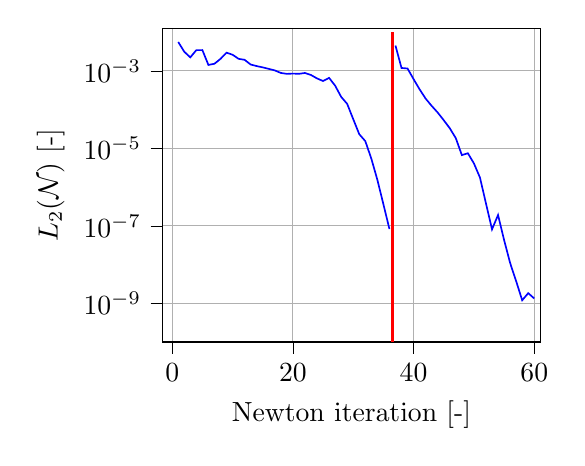
\begin{tikzpicture}

\definecolor{darkgray176}{RGB}{176,176,176}

\begin{axis}[
scale = 0.7, 
xlabel={Newton iteration [-]},
ylabel={$L_2(\mathcal{N})$ [-]},
log basis y={10},
tick align=outside,
tick pos=left,
x grid style={darkgray176},
xmajorgrids,
xmin=-1.6, xmax=61,
xtick style={color=black},
y grid style={darkgray176},
ymajorgrids,
ymin=1e-10, ymax=0.0126591469652629,
ymode=log,
ytick style={color=black}
]
\addplot [semithick, blue]
table {%
1 0.00559062925
2 0.0031301812
3 0.00223868435
4 0.00344552614
5 0.00345346502
6 0.00142879676
7 0.00153028135
8 0.00204665736
9 0.00295736122
10 0.00261947751
11 0.00205372924
12 0.00193612122
13 0.0014638273
14 0.00133445345
15 0.00123537189
16 0.00113096209
17 0.00103079077
18 0.000888034495
19 0.000839491871
20 0.000854236109
21 0.000841152451
22 0.000886753496
23 0.000784952149
24 0.000640534384
25 0.000548232887
26 0.000662010016
27 0.00041684406
28 0.000213944189
29 0.00014094479
30 5.6764511e-05
31 2.32402637e-05
32 1.54177259e-05
33 5.44039411e-06
34 1.5440541e-06
35 3.61030325e-07
36 8.27996193e-08
};
\addplot [semithick, blue]
table {%
37 4.51856345e-03
38 1.19277016e-03
39 1.15480078e-03
40 6.14300157e-04
41 3.34450554e-04
42 1.92823444e-04
43 1.25272275e-04
44 8.40913787e-05
45 5.33996674e-05
46 3.31199208e-05
47 1.8374654e-05
48 6.71014822e-06
49 7.49757004e-06
50 4.09718969e-06
51 1.7709465e-06
52 3.77534086e-07
53 8.12354144e-08
54 1.90755629e-07
55 4.31026373e-08
56 1.10036889e-08
57 3.73119262e-09
58 1.19963723e-09
59 1.82989874e-09
60 1.33381226e-09
};
\addplot [thick, red]
table {%
36.5 1e-10
36.5 0.01
};
\end{axis}

\end{tikzpicture}
 & % This file was created with tikzplotlib v0.10.1.
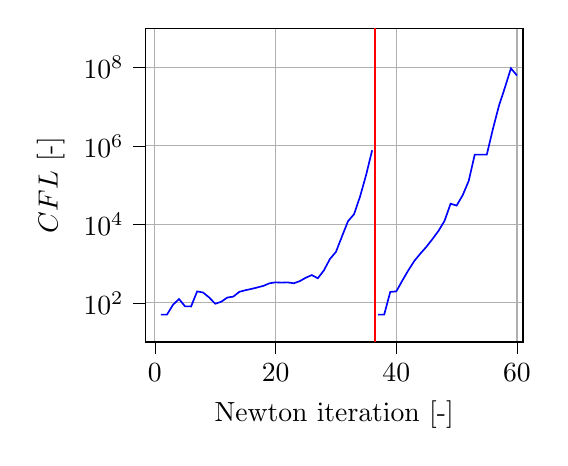
\begin{tikzpicture}
	
\definecolor{darkgray176}{RGB}{176,176,176}

\begin{axis}[
scale = 0.7, 
xlabel={Newton iteration [-]},
ylabel={$CFL$ [-]},
log basis y={10},
tick align=outside,
tick pos=left,
x grid style={darkgray176},
xmajorgrids,
xmin=-1.6, xmax=61,
xtick style={color=black},
y grid style={darkgray176},
ymajorgrids,
ymin=10, ymax=1e9,
ymode=log,
ytick style={color=black}
]
\addplot [semithick, blue]
table {%
1 5.00000000e+01
2 5.00000000e+01
3 8.93020066e+01
4 1.24864170e+02
5 8.11288178e+01
6 8.09423177e+01
7 1.95641165e+02
8 1.82666712e+02
9 1.36579511e+02
10 9.45205681e+01
11 1.06712679e+02
12 1.36109209e+02
13 1.44377046e+02
14 1.90959318e+02
15 2.09472621e+02
16 2.26273129e+02
17 2.47162540e+02
18 2.71181572e+02
19 3.14775456e+02
20 3.32976974e+02
21 3.27229743e+02
22 3.32319620e+02
23 3.15230178e+02
24 3.56112743e+02
25 4.36403525e+02
26 5.09877225e+02
27 4.22246576e+02
28 6.70590011e+02
29 1.30656254e+03
30 1.98326922e+03
31 4.92440537e+03
32 1.20278955e+04
33 1.81305248e+04
34 5.13807377e+04
35 1.81037350e+05
36 7.74260340e+05
};
\addplot [semithick, blue]
table {%
37 5.00000000e+01
38 5.00000000e+01
39 1.89414676e+02
40 1.95642552e+02
41 3.67781401e+02
42 6.75520402e+02
43 1.17168414e+03
44 1.80349700e+03
45 2.68669840e+03
46 4.23089100e+03
47 6.82151911e+03
48 1.22956423e+04
49 3.36696247e+04
50 3.01335194e+04
51 5.51422290e+04
52 1.27574815e+05
53 5.98431190e+05
54 5.98431190e+05
55 5.98431190e+05
56 2.64842538e+06
57 1.03741681e+07
58 3.05945390e+07
59 9.51571986e+07
60 6.23827516e+07

};
\addplot [thick, red]
table {%
36.5 10
36.5 1e9
};
\end{axis}

\end{tikzpicture}

\end{tabular}
}
\only<2>
{
\begin{tabular}{c}
% This file was created with tikzplotlib v0.10.1.
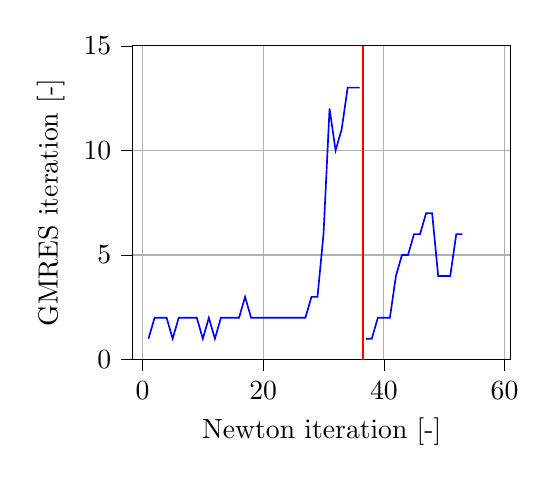
\begin{tikzpicture}

\definecolor{darkgray176}{RGB}{176,176,176}

\begin{axis}[
scale = 0.7, 
xlabel={Newton iteration [-]},
ylabel={GMRES iteration [-]},
log basis y={10},
tick align=outside,
tick pos=left,
x grid style={darkgray176},
xmajorgrids,
xmin=-1.6, xmax=61,
xtick style={color=black},
y grid style={darkgray176},
ymajorgrids,
ymin=0, ymax=15,
%ymode=log,
ytick style={color=black}
]
\addplot [semithick, blue]
table {%
1 1
2 2
3 2
4 2
5 1
6 2
7 2
8 2
9 2
10 1
11 2
12 1
13 2
14 2
15 2
16 2
17 3
18 2
19 2
20 2
21 2
22 2
23 2
24 2
25 2
26 2
27 2
28 3
29 3
30 6
31 12
32 10
33 11
34 13
35 13
36 13
};
\addplot [semithick, blue]
table {%
37 1
38 1
39 2
40 2
41 2
42 4
43 5
44 5
45 6
46 6
47 7
48 7
49 4
50 4
51 4
52 6
53 6
};
\addplot [thick, red]
table {%
36.5 0
36.5 15
};
\end{axis}

\end{tikzpicture}

\end{tabular}
}
\end{center}

\only<3>
{
We have a fast and robust solver for ICP, able to produce meaningful results in 20 minutes of time on a single laptop using 8 OMP threads!
}

\end{frame}

\begin{frame}{Flow fields in ICP: gauge pressure}

\begin{center}
	\begin{tikzpicture}
	\node at (0,0) {\includegraphics[width = \linewidth]{./HS_dp.png}};
	\node at (0,-2.25) {\reflectbox{\includegraphics[width = \linewidth, angle=180, origin=c]{./FS_dp.png}}};
	%\filldraw (-0.05,-2.25) circle (3pt);
	%\filldraw (-0.05,0.) circle (3pt);
	%\filldraw (-7.,-2.2) circle (3pt);
	\filldraw (-5.207716049 ,-2.6578125 ) circle (3pt);
	\filldraw (-4.482407407 ,-2.6578125 ) circle (3pt);
	\filldraw (-3.757098765 ,-2.6578125 ) circle (3pt);
	\filldraw (-3.031790123 ,-2.6578125 ) circle (3pt);
	\filldraw (-2.306481481 ,-2.6578125 ) circle (3pt);
	\filldraw (-1.58117284 ,-2.6578125 ) circle (3pt);
	\end{tikzpicture}
\end{center}

\begin{framed}
\centering
\textbf{The pressure is almost constant everywhere.}
\end{framed}

\end{frame}

\begin{frame}{Flow fields in ICP: temperature}

\begin{center}
	\begin{tikzpicture}
	\node at (0,0) {\includegraphics[width = \linewidth]{./HS_T.png}};
	\node at (0,-2.25) {\reflectbox{\includegraphics[width = \linewidth, angle=180, origin=c]{./FS_T.png}}};
	%\filldraw (-0.05,-2.25) circle (3pt);
	%\filldraw (-0.05,0.) circle (3pt);
	%\filldraw (-7.,-2.2) circle (3pt);
	\filldraw (-5.207716049 ,-2.6578125 ) circle (3pt);
	\filldraw (-4.482407407 ,-2.6578125 ) circle (3pt);
	\filldraw (-3.757098765 ,-2.6578125 ) circle (3pt);
	\filldraw (-3.031790123 ,-2.6578125 ) circle (3pt);
	\filldraw (-2.306481481 ,-2.6578125 ) circle (3pt);
	\filldraw (-1.58117284 ,-2.6578125 ) circle (3pt);
	\end{tikzpicture}
\end{center}

\begin{framed}
\centering
\textbf{Large temperature gradients.}
\end{framed}

\end{frame}

%\begin{frame}{Flow fields in ICP: density}
%
%\begin{center}
%	\begin{tikzpicture}
%	\node at (0,0) {\includegraphics[width = \linewidth]{./HS_rho.png}};
%	\node at (0,-2.25) {\reflectbox{\includegraphics[width = \linewidth, angle=180, origin=c]{./FS_rho.png}}};
%	%\filldraw (-0.05,-2.25) circle (3pt);
%	%\filldraw (-0.05,0.) circle (3pt);
%	%\filldraw (-7.,-2.2) circle (3pt);
%	\filldraw (-5.207716049 ,-2.6578125 ) circle (3pt);
%	\filldraw (-4.482407407 ,-2.6578125 ) circle (3pt);
%	\filldraw (-3.757098765 ,-2.6578125 ) circle (3pt);
%	\filldraw (-3.031790123 ,-2.6578125 ) circle (3pt);
%	\filldraw (-2.306481481 ,-2.6578125 ) circle (3pt);
%	\filldraw (-1.58117284 ,-2.6578125 ) circle (3pt);
%	\end{tikzpicture}
%\end{center}
%\end{frame}

\begin{frame}{Flow fields in ICP: streamlines}

\begin{center}
	\begin{tikzpicture}
		\node at (0,0) {\includegraphics[width = \linewidth]{./HS_Streamlines.png}};
		\node at (0,-2.25) {\reflectbox{\includegraphics[width = \linewidth, angle=180, origin=c]{./FS_Streamlines.png}}};
	\filldraw (-5.207716049 ,-2.6578125 ) circle (3pt);
	\filldraw (-4.482407407 ,-2.6578125 ) circle (3pt);
	\filldraw (-3.757098765 ,-2.6578125 ) circle (3pt);
	\filldraw (-3.031790123 ,-2.6578125 ) circle (3pt);
	\filldraw (-2.306481481 ,-2.6578125 ) circle (3pt);
	\filldraw (-1.58117284 ,-2.6578125 ) circle (3pt);
	\filldraw (-5.207716049 ,0.4078125 ) circle (3pt);
	\filldraw (-4.482407407 ,0.4078125 ) circle (3pt);
	\filldraw (-3.757098765 ,0.4078125 ) circle (3pt);
	\filldraw (-3.031790123 ,0.4078125 ) circle (3pt);
	\filldraw (-2.306481481 ,0.4078125 ) circle (3pt);
	\filldraw (-1.58117284 ,0.4078125 ) circle (3pt);
	\end{tikzpicture}
\end{center}

\begin{framed}
\centering
\textbf{$\nabla \cdot \vecv \simeq 0$}
\end{framed}

\end{frame}

\begin{frame}{Flow fields in ICP: volume power}

\begin{center}
	\begin{tikzpicture}
	\node at (0,0) {\includegraphics[width = \linewidth]{./HS_P.png}};
	\node at (0,-2.25) {\reflectbox{\includegraphics[width = \linewidth, angle=180, origin=c]{./FS_P.png}}};
	%\filldraw (-0.05,-2.25) circle (3pt);
	%\filldraw (-0.05,0.) circle (3pt);
	%\filldraw (-7.,-2.2) circle (3pt);
	\filldraw (-5.207716049 ,-2.6578125 ) circle (3pt);
	\filldraw (-4.482407407 ,-2.6578125 ) circle (3pt);
	\filldraw (-3.757098765 ,-2.6578125 ) circle (3pt);
	\filldraw (-3.031790123 ,-2.6578125 ) circle (3pt);
	\filldraw (-2.306481481 ,-2.6578125 ) circle (3pt);
	\filldraw (-1.58117284 ,-2.6578125 ) circle (3pt);
	\end{tikzpicture}
\end{center}

\begin{framed}
\centering
\textbf{Volume power peak off-axis, where the coupling is the strongest.}
\end{framed}

\end{frame}

\begin{frame}{Flow fields in ICP: Total electric field}

\begin{center}
	\begin{tikzpicture}
	\node at (0,0) {\includegraphics[width = \linewidth]{./HS_E_tot.png}};
	\node at (0,-2.45) {\reflectbox{\includegraphics[width = \linewidth, angle=180, origin=c]{./FS_E_tot.png}}};
%	\filldraw (-3.45,-2.8078125) circle (3pt);
%	\filldraw (-0.5,-2.8078125) circle (3pt);
%	\filldraw (-0.5,-0.2) circle (3pt);
	\filldraw (-3.45,-2.8078125 ) circle (3pt);
	\filldraw (-2.86 ,-2.8078125 ) circle (3pt);
	\filldraw (-2.27 ,-2.8078125 ) circle (3pt);
	\filldraw (-1.68 ,-2.8078125 ) circle (3pt);
	\filldraw (-1.09 ,-2.8078125 ) circle (3pt);
	\filldraw (-0.5,-2.8078125 ) circle (3pt);
	\filldraw (-3.45,-0.2 ) circle (3pt);
	\filldraw (-2.86 ,-0.2 ) circle (3pt);
	\filldraw (-2.27 ,-0.2 ) circle (3pt);
	\filldraw (-1.68 ,-0.2 ) circle (3pt);
	\filldraw (-1.09 ,-0.2 ) circle (3pt);
	\filldraw (-0.5,-0.2 ) circle (3pt);
	\end{tikzpicture}
\end{center}
\end{frame}

\begin{frame}{Flow fields in ICP: Lorentz force}

\begin{center}
	\begin{tikzpicture}
	\node at (0,0) {\includegraphics[width = \linewidth]{./HS_Lorentz.png}};
	\node at (0,-2.25) {\reflectbox{\includegraphics[width = \linewidth, angle=180, origin=c]{./FS_Lorentz.png}}};
	%\filldraw (-0.05,-2.25) circle (3pt);
	%\filldraw (-0.05,0.) circle (3pt);
	%\filldraw (-7.,-2.2) circle (3pt);
	\filldraw (-5.207716049 ,-2.6578125 ) circle (3pt);
	\filldraw (-4.482407407 ,-2.6578125 ) circle (3pt);
	\filldraw (-3.757098765 ,-2.6578125 ) circle (3pt);
	\filldraw (-3.031790123 ,-2.6578125 ) circle (3pt);
	\filldraw (-2.306481481 ,-2.6578125 ) circle (3pt);
	\filldraw (-1.58117284 ,-2.6578125 ) circle (3pt);
	\end{tikzpicture}
\end{center}
\end{frame}

\begin{frame}{Parametric study}

We performed a parametric study of ICP for the parameters used by the experimenters.

\begin{itemize}
\item $Q$ from $\SI{8}{\gram\;\second^{-1}}$ to $\SI{16}{\gram\;\second^{-1}}$.
\item $p_0$ from $\SI{5000}{\pascal}$ to $\SI{20000}{\pascal}$.
\item $P_{tot}$ from $\SI{50}{\kilo\watt}$ to $\SI{200}{\kilo\watt}$.
\item $f$ from $\SI{10}{\kilo\hertz}$, to $\SI{1}{\mega\hertz}$.
\item $S$ from $\SI{0}{\degree}$ to $\SI{20}{\degree}$.
\end{itemize}

\begin{framed}
\centering
\textbf{The complete discussion is in the thesis.}
\end{framed}

\end{frame}

\section{Conclusions and future work}

\begin{frame}{Conclusions}

\begin{description}

\onslide<1->
{
\item[Q1] \textbf{In addition of being precise, can a high-order solver be robust?}
}

\onslide<2->
{
YES! More robust than FV, thanks to the monolithic strategy.
}

\onslide<3-> 
{
\item[Q2] \textbf{Is the developed solver user-friendly?} 
}
\onslide<4->
{

Yes, but there is still some parameter tuning.

However, much easier to use and give meaningful results fast.

A lot of simulations can be performed "eyes closed".
 
}

\onslide<5->
{
\item[Q3] \textbf{Can the new solver be easily adapted to the new experiments performed in ICP facilities?}
}

\onslide<6->
{
We believe so, but there is still much work to do...

Going 2D, 3D, and complex chemistry and radiation for unsteady simulations will need much more computational power.

For supersonic, shock capturing and redesign of the numerical flux.
}

\end{description}

\end{frame}

\begin{frame}{Future work}

Main effort is to put our developments in the ARGO DG solver, which is fully paralleled and equipped shock capturing technologies. (Landry Riou)

We see the following roadmap:
\begin{itemize}
\item Going 3D.

\item Going unsteady (also relieving the average over the induction current period).

\item Development of chemistry (non equilibrium).

\item Development of radiation.

\end{itemize}

%Once these milestones are performed, the path is open to supersonic ICP flows.

\end{frame}


\end{document}